% generated from JIRA project LVV
% using template at /usr/share/miniconda/envs/docsteady-env/lib/python3.7/site-packages/docsteady/templates/tpr.latex.jinja2.
% using docsteady version 2.4
% Please do not edit -- update information in Jira instead
\documentclass[SE,,STR,toc]{lsstdoc}
\usepackage{geometry}
\usepackage{longtable,booktabs}
\usepackage{enumitem}
\usepackage{arydshln}
\usepackage{attachfile}
\usepackage{array}
\usepackage{dashrule}
\usepackage{pdfpages}

\newcolumntype{L}[1]{>{\raggedright\let\newline\\\arraybackslash\hspace{0pt}}p{#1}}

\input meta.tex

\newcommand{\attachmentsUrl}{https://github.com/\gitorg/\lsstDocType-\lsstDocNum/blob/\gitref/attachments}
\providecommand{\tightlist}{
  \setlength{\itemsep}{0pt}\setlength{\parskip}{0pt}}

\setcounter{tocdepth}{4}

\begin{document}

\def\milestoneName{Hexapod Actuator Redesign Verification}
\def\milestoneId{}
\def\product{Hexapod and Rotator}

\setDocCompact{true}

\title{LVV-P95: Hexapod Actuator Redesign Verification Test Plan and Report}
\setDocRef{\lsstDocType-\lsstDocNum}
\date{ 2023-07-11 }
\author{ Kevin Siruno }

% Most recent last
\setDocChangeRecord{
\addtohist{}{2023-02-27}{First draft}{M.Lutfi, K.Siruno}
}

\setDocCurator{M.Lutfi, K.Siruno}
\setDocUpstreamLocation{\url{https://github.com/lsst-dm/\lsstDocType-\lsstDocNum}}
\setDocUpstreamVersion{\vcsRevision}



\setDocAbstract{
This is the test plan and report for
\textbf{ Hexapod Actuator Redesign Verification},
an LSST milestone pertaining to the Data Management Subsystem.\\
This document is based on content automatically extracted from the Jira test database on \docDate.
The most recent change to the document repository was on \vcsDate.
}


\maketitle

\section{Introduction}
\label{sect:intro}


\subsection{Objectives}
\label{sect:objectives}

 The objective of this test plan is to verify the Hexapods requirements
will still be met after changing the design of the encoders on the
hexapod actuators. In order to do this, a series of tests will be
conducted on a single actuator first and then a subset of these tests
will be repeated with the remaining actuators. Once all of the actuators
have been verified, there will be a final verification event for the
entire hexapod.



\subsection{System Overview}
\label{sect:systemoverview}

 \begin{itemize}
\item
  Both the M2 Cell Assembly and Camera use hexapods to facilitate rigid
  body optical positioning relative to the M1M3 Mirror. These hexapods
  utilize identical actuators to facilitate ease of maintainability and
  interchangeability.Actuators incorporate a rotary motor, harmonic
  drive, and a screw. An absolute linear encoder measures the actuator
  length and a relative rotary encoder measures the motor rotation;
  smooth, stiction free flexures provide end rotations; software limits
  electrical limit switches, and hard stops limit travel. Each Actuator
  weighs \textasciitilde{}58.8 kg and measures 620 mm in length.~
\item
  Due to various issues/damages, linear encoders of the hexapod
  actuators will need repair/service/replacement.~

  \begin{itemize}
  \item
    Replacing/servicing the encoder head or tape requires disassembly
    the actuators.
  \item
    Disassembling an actuator requires removing it from the hexapod.
  \item
    Removing the hexapod requires first removing the payload, either the
    camera or M2 mirror cell assembly. ~ ~ ~~
  \end{itemize}
\item
  Hence, all actuators will adopt a modified design to facilitate in
  situ servicing of the linear encoder.
\end{itemize}


\subsection{Document Overview}
\label{sect:docoverview}

This document was generated from Jira, obtaining the relevant information from the
\href{https://jira.lsstcorp.org/secure/Tests.jspa\#/testPlan/LVV-P95}{LVV-P95}
~Jira Test Plan and related Test Cycles (
\href{https://jira.lsstcorp.org/secure/Tests.jspa\#/testCycle/LVV-C188}{LVV-C188}
\href{https://jira.lsstcorp.org/secure/Tests.jspa\#/testCycle/LVV-C196}{LVV-C196}
\href{https://jira.lsstcorp.org/secure/Tests.jspa\#/testCycle/LVV-C197}{LVV-C197}
\href{https://jira.lsstcorp.org/secure/Tests.jspa\#/testCycle/LVV-C254}{LVV-C254}
).

Section \ref{sect:intro} provides an overview of the test campaign, the system under test (\product{}),
the applicable documentation, and explains how this document is organized.
Section \ref{sect:testplan} provides additional information about the test plan, like for example the configuration
used for this test or related documentation.
Section \ref{sect:personnel} describes the necessary roles and lists the individuals assigned to them.

Section \ref{sect:overview} provides a summary of the test results, including an overview in Table \ref{table:summary},
an overall assessment statement and suggestions for possible improvements.
Section \ref{sect:detailedtestresults} provides detailed results for each step in each test case.

The current status of test plan \href{https://jira.lsstcorp.org/secure/Tests.jspa\#/testPlan/LVV-P95}{LVV-P95} in Jira is \textbf{ Approved }.

\subsection{References}
\label{sect:references}
\renewcommand{\refname}{}
\bibliography{lsst,refs,books,refs_ads,local}


\newpage
\section{Test Plan Details}
\label{sect:testplan}


\subsection{Data Collection}

  Observing is not required for this test campaign.

\subsection{Verification Environment}
\label{sect:hwconf}
  The actuator will be verified in the following configuration:

\begin{itemize}
\tightlist
\item
  Set up on the test bench
\item
  Connected to a load cell being supplied air from a pneumatic cylinder
\item
  The air cylinder is connected to an air supply via two valves
\item
  The air valves will be connected to air gauges
\item
  Connected to the control box
\end{itemize}

  \subsection{Entry Criteria}
  \begin{itemize}
\tightlist
\item
  The test bench is fully set up with redesigned actuator installed in
  it.~
\item
  Control box fully set up.~
\item
  Safety hazards are mitigated with appropriate measures.~
\end{itemize}

  \subsection{Exit Criteria}
  The data collected during the execution of this test case has been post
processed, analyzed, and compared to the previous execution results from
the vendors acceptance test report. The summary of the results is
captured in this test plan.~


\subsection{Related Documentation}

Docushare collection where additional relevant documentation can be found:

\begin{itemize}
\item Each test includes a link to a docushare collection that contains all of
the test results, raw data and relevant documentation to the test.
However, the parent docushare collection to all of those collections can
be found here:
\url{https://docushare.lsst.org/docushare/dsweb/View/Collection-13951}
\end{itemize}


\subsection{PMCS Activity}

Primavera milestones related to the test campaign:
\begin{itemize}
\item None
\end{itemize}


\newpage
\section{Personnel}
\label{sect:personnel}

The personnel involved in the test campaign is shown in the following table.

{\small
\begin{longtable}{p{3cm}p{3cm}p{3cm}p{6cm}}
\hline
\multicolumn{2}{r}{T. Plan \href{https://jira.lsstcorp.org/secure/Tests.jspa\#/testPlan/LVV-P95}{LVV-P95} owner:} &
\multicolumn{2}{l}{\textbf{ Kevin Siruno } }\\\hline
\multicolumn{2}{r}{T. Cycle \href{https://jira.lsstcorp.org/secure/Tests.jspa\#/testCycle/LVV-C188}{LVV-C188} owner:} &
\multicolumn{2}{l}{\textbf{
Mostafa Lutfi }
} \\\hline
\textbf{Test Cases} & \textbf{Assigned to} & \textbf{Executed by} & \textbf{Additional Test Personnel} \\ \hline
\href{https://jira.lsstcorp.org/secure/Tests.jspa#/testCase/LVV-T2531}{LVV-T2531}
& {\small Kevin Siruno } & {\small Kevin Siruno } &
\begin{minipage}[]{6cm}
\smallskip
{\small (2) Mechanical Personnel\\
(1) Electrical Technician }
\medskip
\end{minipage}
\\ \hline
\href{https://jira.lsstcorp.org/secure/Tests.jspa#/testCase/LVV-T2426}{LVV-T2426}
& {\small Mostafa Lutfi } & {\small Kevin Siruno } &
\begin{minipage}[]{6cm}
\smallskip
{\small (1) Systems Engineer\\
(1) Electrical Technician }
\medskip
\end{minipage}
\\ \hline
\href{https://jira.lsstcorp.org/secure/Tests.jspa#/testCase/LVV-T2427}{LVV-T2427}
& {\small Mostafa Lutfi } & {\small Kevin Siruno } &
\begin{minipage}[]{6cm}
\smallskip
{\small (1) Systems Engineer\\
(1) Electrical Technician }
\medskip
\end{minipage}
\\ \hline
\href{https://jira.lsstcorp.org/secure/Tests.jspa#/testCase/LVV-T2428}{LVV-T2428}
& {\small Mostafa Lutfi } & {\small Kevin Siruno } &
\begin{minipage}[]{6cm}
\smallskip
{\small (1) Systems Engineer\\
(1) Electrical Technician }
\medskip
\end{minipage}
\\ \hline
\href{https://jira.lsstcorp.org/secure/Tests.jspa#/testCase/LVV-T2437}{LVV-T2437}
& {\small Kevin Siruno } & {\small Kevin Siruno } &
\begin{minipage}[]{6cm}
\smallskip
{\small (1) Systems Engineer\\
(1) Electrical Technician }
\medskip
\end{minipage}
\\ \hline
\href{https://jira.lsstcorp.org/secure/Tests.jspa#/testCase/LVV-T2432}{LVV-T2432}
& {\small Mostafa Lutfi } & {\small Kevin Siruno } &
\begin{minipage}[]{6cm}
\smallskip
{\small (1) Systems Engineer\\
(1) Electrical Technician }
\medskip
\end{minipage}
\\ \hline
\href{https://jira.lsstcorp.org/secure/Tests.jspa#/testCase/LVV-T2434}{LVV-T2434}
& {\small Mostafa Lutfi } & {\small Kevin Siruno } &
\begin{minipage}[]{6cm}
\smallskip
{\small (1) Systems Engineer\\
(1) Electrical Technician }
\medskip
\end{minipage}
\\ \hline
\href{https://jira.lsstcorp.org/secure/Tests.jspa#/testCase/LVV-T2436}{LVV-T2436}
& {\small Mostafa Lutfi } & {\small Kevin Siruno } &
\begin{minipage}[]{6cm}
\smallskip
{\small (1) Systems Engineer\\
(1) Electrical Technician }
\medskip
\end{minipage}
\\ \hline
\href{https://jira.lsstcorp.org/secure/Tests.jspa#/testCase/LVV-T2435}{LVV-T2435}
& {\small Kevin Siruno } & {\small Kevin Siruno } &
\begin{minipage}[]{6cm}
\smallskip
{\small (1) Systems Engineer\\
(1) Electrical Technician }
\medskip
\end{minipage}
\\ \hline
\href{https://jira.lsstcorp.org/secure/Tests.jspa#/testCase/LVV-T2431}{LVV-T2431}
& {\small Kevin Siruno } & {\small Kevin Siruno } &
\begin{minipage}[]{6cm}
\smallskip
{\small (1) Systems Engineer\\
(1) Electrical Technician }
\medskip
\end{minipage}
\\ \hline
\href{https://jira.lsstcorp.org/secure/Tests.jspa#/testCase/LVV-T2844}{LVV-T2844}
& {\small Kevin Siruno } & {\small Kevin Siruno } &
\begin{minipage}[]{6cm}
\smallskip
{\small (1) Systems Engineer\\
(1) Electrical Technician }
\medskip
\end{minipage}
\\ \hline
\multicolumn{2}{r}{T. Cycle \href{https://jira.lsstcorp.org/secure/Tests.jspa\#/testCycle/LVV-C196}{LVV-C196} owner:} &
\multicolumn{2}{l}{\textbf{
Kevin Siruno }
} \\\hline
\textbf{Test Cases} & \textbf{Assigned to} & \textbf{Executed by} & \textbf{Additional Test Personnel} \\ \hline
\href{https://jira.lsstcorp.org/secure/Tests.jspa#/testCase/LVV-T2531}{LVV-T2531}
& {\small Kevin Siruno } & {\small  } &
\begin{minipage}[]{6cm}
\smallskip
{\small (2) Mechanical Personnel\\
(1) Electrical Technician }
\medskip
\end{minipage}
\\ \hline
\href{https://jira.lsstcorp.org/secure/Tests.jspa#/testCase/LVV-T2428}{LVV-T2428}
& {\small Mostafa Lutfi } & {\small  } &
\begin{minipage}[]{6cm}
\smallskip
{\small (1) Systems Engineer\\
(1) Electrical Technician }
\medskip
\end{minipage}
\\ \hline
\href{https://jira.lsstcorp.org/secure/Tests.jspa#/testCase/LVV-T2432}{LVV-T2432}
& {\small Mostafa Lutfi } & {\small  } &
\begin{minipage}[]{6cm}
\smallskip
{\small (1) Systems Engineer\\
(1) Electrical Technician }
\medskip
\end{minipage}
\\ \hline
\href{https://jira.lsstcorp.org/secure/Tests.jspa#/testCase/LVV-T2437}{LVV-T2437}
& {\small Kevin Siruno } & {\small  } &
\begin{minipage}[]{6cm}
\smallskip
{\small (1) Systems Engineer\\
(1) Electrical Technician }
\medskip
\end{minipage}
\\ \hline
\href{https://jira.lsstcorp.org/secure/Tests.jspa#/testCase/LVV-T2434}{LVV-T2434}
& {\small Mostafa Lutfi } & {\small  } &
\begin{minipage}[]{6cm}
\smallskip
{\small (1) Systems Engineer\\
(1) Electrical Technician }
\medskip
\end{minipage}
\\ \hline
\href{https://jira.lsstcorp.org/secure/Tests.jspa#/testCase/LVV-T2436}{LVV-T2436}
& {\small Mostafa Lutfi } & {\small  } &
\begin{minipage}[]{6cm}
\smallskip
{\small (1) Systems Engineer\\
(1) Electrical Technician }
\medskip
\end{minipage}
\\ \hline
\href{https://jira.lsstcorp.org/secure/Tests.jspa#/testCase/LVV-T2435}{LVV-T2435}
& {\small Kevin Siruno } & {\small  } &
\begin{minipage}[]{6cm}
\smallskip
{\small (1) Systems Engineer\\
(1) Electrical Technician }
\medskip
\end{minipage}
\\ \hline
\multicolumn{2}{r}{T. Cycle \href{https://jira.lsstcorp.org/secure/Tests.jspa\#/testCycle/LVV-C197}{LVV-C197} owner:} &
\multicolumn{2}{l}{\textbf{
Kevin Siruno }
} \\\hline
\textbf{Test Cases} & \textbf{Assigned to} & \textbf{Executed by} & \textbf{Additional Test Personnel} \\ \hline
\multicolumn{2}{r}{T. Cycle \href{https://jira.lsstcorp.org/secure/Tests.jspa\#/testCycle/LVV-C254}{LVV-C254} owner:} &
\multicolumn{2}{l}{\textbf{
Mostafa Lutfi }
} \\\hline
\textbf{Test Cases} & \textbf{Assigned to} & \textbf{Executed by} & \textbf{Additional Test Personnel} \\ \hline
\href{https://jira.lsstcorp.org/secure/Tests.jspa#/testCase/LVV-T2805}{LVV-T2805}
& {\small Kevin Siruno } & {\small Kevin Siruno } &
\begin{minipage}[]{6cm}
\smallskip
{\small (2) Systems Engineer\\
(1) Electrical Technician }
\medskip
\end{minipage}
\\ \hline
\href{https://jira.lsstcorp.org/secure/Tests.jspa#/testCase/LVV-T2531}{LVV-T2531}
& {\small Kevin Siruno } & {\small Kevin Siruno } &
\begin{minipage}[]{6cm}
\smallskip
{\small (2) Mechanical Personnel\\
(1) Electrical Technician }
\medskip
\end{minipage}
\\ \hline
\href{https://jira.lsstcorp.org/secure/Tests.jspa#/testCase/LVV-T2427}{LVV-T2427}
& {\small Mostafa Lutfi } & {\small Kevin Siruno } &
\begin{minipage}[]{6cm}
\smallskip
{\small (1) Systems Engineer\\
(1) Electrical Technician }
\medskip
\end{minipage}
\\ \hline
\href{https://jira.lsstcorp.org/secure/Tests.jspa#/testCase/LVV-T2428}{LVV-T2428}
& {\small Mostafa Lutfi } & {\small Kevin Siruno } &
\begin{minipage}[]{6cm}
\smallskip
{\small (1) Systems Engineer\\
(1) Electrical Technician }
\medskip
\end{minipage}
\\ \hline
\href{https://jira.lsstcorp.org/secure/Tests.jspa#/testCase/LVV-T2437}{LVV-T2437}
& {\small Kevin Siruno } & {\small Kevin Siruno } &
\begin{minipage}[]{6cm}
\smallskip
{\small (1) Systems Engineer\\
(1) Electrical Technician }
\medskip
\end{minipage}
\\ \hline
\href{https://jira.lsstcorp.org/secure/Tests.jspa#/testCase/LVV-T2432}{LVV-T2432}
& {\small Mostafa Lutfi } & {\small Kevin Siruno } &
\begin{minipage}[]{6cm}
\smallskip
{\small (1) Systems Engineer\\
(1) Electrical Technician }
\medskip
\end{minipage}
\\ \hline
\href{https://jira.lsstcorp.org/secure/Tests.jspa#/testCase/LVV-T2434}{LVV-T2434}
& {\small Mostafa Lutfi } & {\small Kevin Siruno } &
\begin{minipage}[]{6cm}
\smallskip
{\small (1) Systems Engineer\\
(1) Electrical Technician }
\medskip
\end{minipage}
\\ \hline
\href{https://jira.lsstcorp.org/secure/Tests.jspa#/testCase/LVV-T2436}{LVV-T2436}
& {\small Mostafa Lutfi } & {\small Kevin Siruno } &
\begin{minipage}[]{6cm}
\smallskip
{\small (1) Systems Engineer\\
(1) Electrical Technician }
\medskip
\end{minipage}
\\ \hline
\href{https://jira.lsstcorp.org/secure/Tests.jspa#/testCase/LVV-T2435}{LVV-T2435}
& {\small Kevin Siruno } & {\small Kevin Siruno } &
\begin{minipage}[]{6cm}
\smallskip
{\small (1) Systems Engineer\\
(1) Electrical Technician }
\medskip
\end{minipage}
\\ \hline
\end{longtable}
}

\newpage

\section{Test Campaign Overview}
\label{sect:overview}

\subsection{Summary}
\label{sect:summarytable}

{\small
\begin{longtable}{p{2cm}cp{2.3cm}p{8.6cm}p{2.3cm}}
\toprule
\multicolumn{2}{r}{ T. Plan \href{https://jira.lsstcorp.org/secure/Tests.jspa\#/testPlan/LVV-P95}{LVV-P95}:} &
\multicolumn{2}{p{10.9cm}}{\textbf{ Hexapod Actuator Redesign Verification }} & Approved \\\hline
\multicolumn{2}{r}{ T. Cycle \href{https://jira.lsstcorp.org/secure/Tests.jspa\#/testCycle/LVV-C188}{LVV-C188}:} &
\multicolumn{2}{p{10.9cm}}{\textbf{ Single Hexapod Actuator Redesign Verification }} & Done \\\hline
\textbf{Test Cases} &  \textbf{Ver.} & \textbf{Status} & \textbf{Comment} & \textbf{Issues} \\\toprule
\href{https://jira.lsstcorp.org/secure/Tests.jspa#/testCase/LVV-T2531}{LVV-T2531}
&  1
& Pass &
\begin{minipage}[]{9cm}
\smallskip
When determining the center stroke position, the internal rotary encoder
reported -22.008mm. However, during the Unmodified Single Hexapod
Actuator Redesign Verification campaign, the center stroke position was
seen to be -40.202mm. Since the external linear encoders reported to be
about 39.5mm during both campaigns, this change seen in the center
stroke position was determined to be okay. One possible explanation for
why this was changed is because the actuator may have been rotated
during the modification which would have resulted in a different
internal rotary encoder reading.
\medskip
\end{minipage}
&   \\\hline
\href{https://jira.lsstcorp.org/secure/Tests.jspa#/testCase/LVV-T2426}{LVV-T2426}
&  1
& Pass &
\begin{minipage}[]{9cm}
\smallskip
In order to prevent over stressing the actuator, this test was only
conducted on the modified actuator. During this test, there were no
obvious signs of damage so this test was considered passed. The data
taken from this test case be seen in the attached \emph{200\% Proofing
Test Results - Modified Actuator.xlsx}.
\medskip
\end{minipage}
&   \\\hline
\href{https://jira.lsstcorp.org/secure/Tests.jspa#/testCase/LVV-T2427}{LVV-T2427}
&  1
& Pass &
\begin{minipage}[]{9cm}
\smallskip
During the Unmodified Actuator Verification campaign, the internal
rotary encoder reading was not recorded and so the displacement as
measured by the external linear encoders were recorded instead. However,
during this Modified Actuator Verification campaign, the back driving
test was able to be conducted using the readings from the internal
rotary encoder. As a result, it can be seen in the steps below that the
back driving measured during this test was measured to be under 10
counts for both tension and compression load. The data as measured by
the external linear encoders can be seen in the attached \emph{Back
Drive Test Results - Unmodified Actuator (1).xlsm} excel file.
\medskip
\end{minipage}
&   \\\hline
\href{https://jira.lsstcorp.org/secure/Tests.jspa#/testCase/LVV-T2428}{LVV-T2428}
&  1
& Pass &
\begin{minipage}[]{9cm}
\smallskip
The actuator was placed as close to the positive limit switch as
possible when extended and as close to the negative limit switch as
possible when retracted.\\
As a reminder, the reported position of the rotary encoder were
different after the actuator modifications.\\
Negative Limit Switch:

\begin{itemize}
\tightlist
\item
  Copley Software: Active Load Position = \textbf{-36.03mm or
  -36003000counts}
\end{itemize}

Zero Position:

\begin{itemize}
\tightlist
\item
  Copley Software: Active Load Position = \textbf{-22.008mm or -2200875
  counts}
\end{itemize}

Positive Limit Switch:

\begin{itemize}
\tightlist
\item
  Copley Software: Active Load Position = \textbf{-7.515mm or -7515000
  counts}
\end{itemize}

In conclusion, the stiffness of the actuator was seen in the following
positions as follows:

\begin{itemize}
\tightlist
\item
  Zero Position = 101.6N/um
\item
  Negative Limit Switch = 101.4N/um
\item
  Positive Limit Switch = 101.6N/um
\end{itemize}

The results from both the unmodified and modified actuator tests have
been uploaded into docushare. As seen in the Results Summary sheet,
Moog's results showed that the stiffness of the actuator was on average
117N/um. The results from the unmodified actuator stiffness test showed
that the actuator was on average 130N/um. It can be seen that the
actuator is a lot less stiff than MOOG's original results and the
results obtained from the unmodified test. It can be seen in the results
of the attached document that there is not only larger displacement in
the modified actuator test results, but there is a larger delta between
the two encoder positions. An explanation for this may be due to the
fact that the modified design includes a cutout meant for the external
encoder housing that is causing a twisting moment. As a result, this is
causing displacement at a higher rate for one encoder than the other.
This can be seen in the graphs plotting velocity of the encoders vs time
on the Velocity Graphs\emph{~}sheet of the
\href{https://docushare.lsst.org/docushare/dsweb/Services/Document-55068}{\emph{Stiffness
Test Results Modified vs UnModified.xlsx}}file.
\medskip
\end{minipage}
&   \\\hline
\href{https://jira.lsstcorp.org/secure/Tests.jspa#/testCase/LVV-T2437}{LVV-T2437}
&  1
& Pass &
\begin{minipage}[]{9cm}
\smallskip
Similar to MOOG's original procedure and the unmodified actuator
movement test, the settling time started when the actuator had reached
its commanded position of +/-5mm and ended when the displacement was
within 0.001mm of that position. As seen in the results of this test
case, the actuator was capable of accurately reaching the +/-5mm
commanded position and the settling time was again seen to be less than
2 seconds. This can be seen in the attached
\href{https://docushare.lsst.org/docushare/dsweb/Services/Document-55079}{\emph{Movement
Test Results - Modified Actuator.xlsx}}\emph{~}excel file.\\
The results of both tension and compression were combined in order to
observe the actuator movement throughout the full test.
\medskip
\end{minipage}
&   \\\hline
\href{https://jira.lsstcorp.org/secure/Tests.jspa#/testCase/LVV-T2432}{LVV-T2432}
&  1
& Pass &
\begin{minipage}[]{9cm}
\smallskip
The purpose of this test was to verify that the limit switches would
prevent the actuator from moving beyond an unsafe range of motion. The
actuator can incur serious damage if allowed to move beyond +/-15mm.
Therefore, the limits switches were set to be around +/-14.3mm, which is
within the +/-15mm but capable of allowing the overall hexapod range of
motion requirements to still be met.\\
During the Modified Actuator Verification Campaign, a new set of limit
switches had to be installed. However, the paddles on the limit switches
were not bent exactly like the original limit switches. As a result, the
limit switches had to be manually readjusted to trigger as close as
possible to the original +/-14.3mm. The calculations that were used to
determine the necessary adjustment are seen in the attached document.\\
Overall, this test was considered to be passed as the limit switches
were readjusted and seen to stop the actuator from moving beyond its
range of motion. The full range of motion is listed below:\\
Negative Limit Switch:

\begin{itemize}
\tightlist
\item
  Copley Software: Active Load Position = \textbf{-36.03mm or
  -36003000counts}
\item
  Encoder A (D13B) = 53.28mm
\item
  Encoder B (D0BD) = 53.73mm
\end{itemize}

Zero Position:

\begin{itemize}
\tightlist
\item
  Copley Software: Active Load Position = \textbf{-22.008mm or -2200875
  counts}
\item
  Encoder A (D13B) = 39.4mm
\item
  Encoder B (D0BD) = 39.5mm
\end{itemize}

Positive Limit Switch:

\begin{itemize}
\tightlist
\item
  Copley Software: Active Load Position = \textbf{-7.515mm or
  -7515000counts}
\item
  Encoder A (D13B) = 24.78mm
\item
  Encoder B (D0BD) = 25.23mm
\end{itemize}

In conclusion, the stiffness of the actuator was seen in the following
positions as follows:

\begin{itemize}
\tightlist
\item
  Zero Position = 101.6N/um
\item
  Negative Limit Switch = 101.4N/um
\item
  Positive Limit Switch = 101.6N/um~
\end{itemize}

\href{https://docushare.lsst.org/docushare/dsweb/Services/Document-55106}{Encoder
Range Comparison (unmod vs mod).xlsx}
\medskip
\end{minipage}
&   \\\hline
\href{https://jira.lsstcorp.org/secure/Tests.jspa#/testCase/LVV-T2434}{LVV-T2434}
&  1
& Pass &
\begin{minipage}[]{9cm}
\smallskip
The expected result of this test was that given 100nm moves with any
load, the actuator would reach the commanded position within 50nm.
However, there were some deviations to the 100nm moves seen to be
greater than 50nm. This was expected as MOOG's original test results
described similar issues related to excessive noise on the load cell and
on the external encoders. Additionally, a load compensation could not be
performed with the displacement being measured in nm's. Therefore, since
the encoders were seen to be able to track the actuator movement closely
and in the correct commanded direction, this test was passed.
\medskip
\end{minipage}
&   \\\hline
\href{https://jira.lsstcorp.org/secure/Tests.jspa#/testCase/LVV-T2436}{LVV-T2436}
&  1
& Pass &
\begin{minipage}[]{9cm}
\smallskip
For this we started at the Zero Position:\\

\begin{itemize}
\tightlist
\item
  Copley Software: Active Load Position = \textbf{-22.008mm or -2200875
  counts}
\item
  Encoder A (D13B) = 39.4mm
\item
  Encoder B (D0BD) = 39.5mm
\end{itemize}

During this test, it can be seen in the results that there were
variations in the applied load that may have impacted the results of
this test. As a result of the noise, there were outliers to the expected
accuracy, specifically for the larger moves in mm. For the smaller moves
in um, the accuracy was less than the expected error. However, this was
expected as MOOG's original test report cites the same variation when
applying load. Therefore, load compensation was applied to the results
in an effort to reduce the noise's impact on the results. Applying load
compensation improved the overall results, but there were still some
outliers that were greater than the expected 17um for the large moves:

\begin{itemize}
\tightlist
\item
  Large scale accuracy maximum error - Tension = \textbf{22.65um}
\item
  Large scale accuracy maximum error - Compression = \textbf{24.76um}
\item
  Large scale accuracy maximum error - Zero = \textbf{41.54um}
\end{itemize}

For the smaller moves, the maximum error was less than the expected
20um:

\begin{itemize}
\tightlist
\item
  Small scale accuracy maximum error - Tension = 12.25um
\item
  Small scale accuracy maximum error - Compression = 17.7um
\item
  Small scale accuracy maximum error - Zero = 16.8um
\end{itemize}

Overall, the absolute accuracy of the actuators are not critical for the
operation of the hexapods. Therefore, the results have been recorded and
this test was marked as passed.
\medskip
\end{minipage}
&   \\\hline
\href{https://jira.lsstcorp.org/secure/Tests.jspa#/testCase/LVV-T2435}{LVV-T2435}
&  1
& Pass &
\begin{minipage}[]{9cm}
\smallskip
Similar to the execution of this test with the unmodified actuator, the
repeatability was determined by observing the measured displacement of
the actuator after completing a move and settle. As seen in the final
comparison of results in the
\href{https://docushare.lsst.org/docushare/dsweb/Services/Document-55071}{\emph{Repeatibility
Test Results -Modified vs UnModified.xlsx}} document, both the modified
and unmodified actuator had a repeatibility of less than 5um.\\
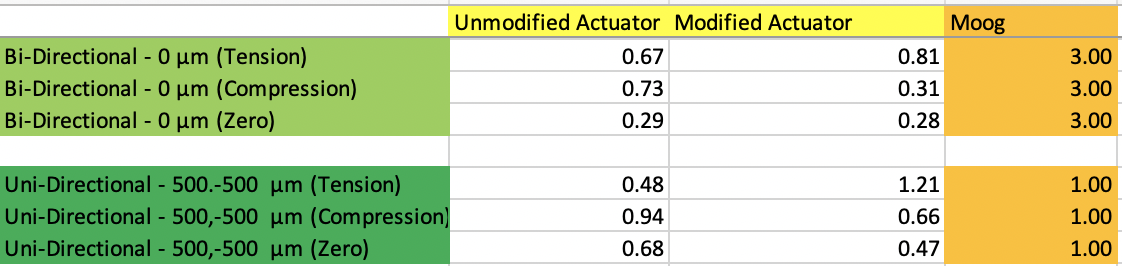
\includegraphics[width=4.42708in]{jira_imgs/4106.png}
\medskip
\end{minipage}
&   \\\hline
\href{https://jira.lsstcorp.org/secure/Tests.jspa#/testCase/LVV-T2431}{LVV-T2431}
&  1
& Pass &
\begin{minipage}[]{9cm}
\smallskip
An initial sequence of 20 moves was performed and the actuator
temperature was seen to rise from 23.65degC to 28.5degC without any
indication of stopping. The operational limit of the actuator drive was
cited to be from 0 to 40degC. Therefore, we added a fan to prevent the
temperature from increasing beyond 30degC during the test. During the
tests, the temperature readings could not be exported while the
telemetry was being displayed in real time. Therefore, the temperature
telemetry was left on display to verify the temperature never reached
above 30degC. As a result of this test, the temperature never rose
beyond 30degC with the fan on the actuator and there were no obvious
damage/faults on the actuator.~
\medskip
\end{minipage}
&   \\\hline
\href{https://jira.lsstcorp.org/secure/Tests.jspa#/testCase/LVV-T2844}{LVV-T2844}
&  1
& Pass &
\begin{minipage}[]{9cm}
\smallskip
The purpose of this test was to ensure that the application of load was
not affecting the results by causing the encoders to separate too far
from the encoder tapes. As a result of this test, it was visually
confirmed that the encoders remained properly spaced during commanded
moves with load applied.\\
As seen in the videos included in the docushare collection, the encoders
visually remain the same distance away from the encoder tape. However,
the real indication that the encoders are sufficiently spaced is the LED
on the encoder. The LED turns blue when the encoder is the correct
distance away from the encoder tape. If the LED is green, orange, or
red, this indicates the signal is not as strong (with red being the
worst). However, since the encoders were seen to be blue for the full
test, this test can be considered to be passed.
\medskip
\end{minipage}
&   \\\hline
\multicolumn{2}{r}{ T. Cycle \href{https://jira.lsstcorp.org/secure/Tests.jspa\#/testCycle/LVV-C196}{LVV-C196}:} &
\multicolumn{2}{p{10.9cm}}{\textbf{ Hexapod Actuator Acceptance Test }} & Not Executed \\\hline
\textbf{Test Cases} &  \textbf{Ver.} & \textbf{Status} & \textbf{Comment} & \textbf{Issues} \\\toprule
\href{https://jira.lsstcorp.org/secure/Tests.jspa#/testCase/LVV-T2531}{LVV-T2531}
&  1
& Not Executed &
\begin{minipage}[]{9cm}
\smallskip

\medskip
\end{minipage}
&   \\\hline
\href{https://jira.lsstcorp.org/secure/Tests.jspa#/testCase/LVV-T2428}{LVV-T2428}
&  1
& Not Executed &
\begin{minipage}[]{9cm}
\smallskip

\medskip
\end{minipage}
&   \\\hline
\href{https://jira.lsstcorp.org/secure/Tests.jspa#/testCase/LVV-T2432}{LVV-T2432}
&  1
& Not Executed &
\begin{minipage}[]{9cm}
\smallskip

\medskip
\end{minipage}
&   \\\hline
\href{https://jira.lsstcorp.org/secure/Tests.jspa#/testCase/LVV-T2437}{LVV-T2437}
&  1
& Not Executed &
\begin{minipage}[]{9cm}
\smallskip

\medskip
\end{minipage}
&   \\\hline
\href{https://jira.lsstcorp.org/secure/Tests.jspa#/testCase/LVV-T2434}{LVV-T2434}
&  1
& Not Executed &
\begin{minipage}[]{9cm}
\smallskip

\medskip
\end{minipage}
&   \\\hline
\href{https://jira.lsstcorp.org/secure/Tests.jspa#/testCase/LVV-T2436}{LVV-T2436}
&  1
& Not Executed &
\begin{minipage}[]{9cm}
\smallskip

\medskip
\end{minipage}
&   \\\hline
\href{https://jira.lsstcorp.org/secure/Tests.jspa#/testCase/LVV-T2435}{LVV-T2435}
&  1
& Not Executed &
\begin{minipage}[]{9cm}
\smallskip

\medskip
\end{minipage}
&   \\\hline
\multicolumn{2}{r}{ T. Cycle \href{https://jira.lsstcorp.org/secure/Tests.jspa\#/testCycle/LVV-C197}{LVV-C197}:} &
\multicolumn{2}{p{10.9cm}}{\textbf{ Hexapod System Level Acceptance Test }} & Not Executed \\\hline
\textbf{Test Cases} &  \textbf{Ver.} & \textbf{Status} & \textbf{Comment} & \textbf{Issues} \\\toprule
\multicolumn{2}{r}{ T. Cycle \href{https://jira.lsstcorp.org/secure/Tests.jspa\#/testCycle/LVV-C254}{LVV-C254}:} &
\multicolumn{2}{p{10.9cm}}{\textbf{ Unmodified Single Hexapod Actuator Redesign Verification }} & Done \\\hline
\textbf{Test Cases} &  \textbf{Ver.} & \textbf{Status} & \textbf{Comment} & \textbf{Issues} \\\toprule
\href{https://jira.lsstcorp.org/secure/Tests.jspa#/testCase/LVV-T2805}{LVV-T2805}
&  1
& Pass &
\begin{minipage}[]{9cm}
\smallskip
The test was executed initially by applying steps for forces in
compression first and then tension. When applying forces in compression,
we started with the supply pressure = 20psi. As we applied more load in
compression, we also gradually increased the air supply. By doing this,
we were able to safely observe the rate that the load was being applied
at lower pressures first before increasing to the maximum air pressure.
As a result, we determined that load could be applied safely onto the
actuator and at least 90psi is required to be able to apply a load of
+/-60kN.
\medskip
\end{minipage}
&   \\\hline
\href{https://jira.lsstcorp.org/secure/Tests.jspa#/testCase/LVV-T2531}{LVV-T2531}
&  1
& Pass &
\begin{minipage}[]{9cm}
\smallskip
This test case includes the installation of the actuator onto the test
rig and validation of the Copley software control. As seen in the
results, we validated the position of the positive and negative limit
switches. After determining the positions of those, we calculated the
zero position to be exactly half the distance between the two limit
switches = \textbf{-40202000 counts or -40.202mm.}
\medskip
\end{minipage}
&   \\\hline
\href{https://jira.lsstcorp.org/secure/Tests.jspa#/testCase/LVV-T2427}{LVV-T2427}
&  1
& Pass &
\begin{minipage}[]{9cm}
\smallskip
The proofing 200\% load test will not be conducted as part of this test
cycle. Therefore, it was not a pre-requisite to executing this test
case. See
\href{https://jira.lsstcorp.org/secure/Tests.jspa\#/testPlayer/testExecution/LVV-E2728}{LVV-E2728}.\\[2\baselineskip]During
MOOG's original test, the back driving was determined by reading the
internal rotary encoder and therefore was measured in counts. During
this test, the displacement was measured by the external linear encoders
and was measured in mm. As seen in the results, the total displacement
by either encoder when applying loads never exceeded 0.32mm. The results
were agreed to be sufficient to repeat this test on the modified
actuator.
\medskip
\end{minipage}
&   \\\hline
\href{https://jira.lsstcorp.org/secure/Tests.jspa#/testCase/LVV-T2428}{LVV-T2428}
&  1
& Pass &
\begin{minipage}[]{9cm}
\smallskip
Moog's results already determined that, effective serial test stand
stiffness was very high and had less than 1\% impact on the measured
stiffness of the actuators. We also got similar results while
calculating stiffness with surrogate.\\
In conclusion, the stiffness of the actuator was seen in the following
positions as follows:

\begin{itemize}
\tightlist
\item
  Zero Position = 131.6 N/um
\item
  Extended Position (Positive Limit position) = 135.39 N/um
\item
  Retracted Position (Negative Limit position) = 126.69 N/um
\end{itemize}

The calculation of these final results can be found in the
\href{https://docushare.lsst.org/docushare/dsweb/Services/Document-55068}{\emph{Stiffness
Test Results Modified vs Unmodified.xlsx}}\emph{~}document
\medskip
\end{minipage}
&   \\\hline
\href{https://jira.lsstcorp.org/secure/Tests.jspa#/testCase/LVV-T2437}{LVV-T2437}
&  1
& Pass &
\begin{minipage}[]{9cm}
\smallskip
During the test, the velocity and acceleration limits could not be
changed in the Copley control software. However, the limits were already
set to the desired velocity and acceleration. As a result, we verified
that the actuator was still capable of meeting the minimum velocity of
the 0.342mm/s. The settling time was also verified by this test.\\
According to MOOG's original procedure, the settling time started when
the actuator had reached its commanded position of +/-5mm and ended when
the displacement was within 0.001mm of that commanded position. As seen
in the results of this test case, the settling time was always seen to
be less than 2 seconds. This is supported by the raw data as seen in the
\href{https://docushare.lsst.org/docushare/dsweb/Services/Document-55090}{\emph{Movement
Test Results - Unmodified Actuator.xlsx}}\emph{~}document.
\medskip
\end{minipage}
&   \\\hline
\href{https://jira.lsstcorp.org/secure/Tests.jspa#/testCase/LVV-T2432}{LVV-T2432}
&  1
& Pass &
\begin{minipage}[]{9cm}
\smallskip
The original scope of this test was to verify the position of the
positive and negative limit switches using the Copley Control software.
There were additional steps involved based on MOOG's original procedure
that cited that the software limit switches would be set and needed to
be adjusted in order to do so. However, MOOG used additional software to
set and adjust the software limit switches of the actuator. Therefore,
those steps were skipped for the purposes of this test and only the
steps related to determining the physical limit switches were tested.~
\medskip
\end{minipage}
&   \\\hline
\href{https://jira.lsstcorp.org/secure/Tests.jspa#/testCase/LVV-T2434}{LVV-T2434}
&  1
& Pass &
\begin{minipage}[]{9cm}
\smallskip
The test was performed starting from the zero position (Active Copley =
-40.202mm).\\[2\baselineskip]The expected result of this test was that
given 100nm moves with any load, the actuator would reach the commanded
position within 50nm. However, there were some deviations to the 100nm
moves seen to be greater than 50nm. This was expected as MOOG's original
test results described similar issues related to excessive noise on the
load cell and on the external encoders. Additionally, a load
compensation could not be performed with the displacement being measured
in nm's. Therefore, since the encoders were seen to be able to track the
actuator movement closely and in the correct commanded direction, this
test was passed.
\medskip
\end{minipage}
&   \\\hline
\href{https://jira.lsstcorp.org/secure/Tests.jspa#/testCase/LVV-T2436}{LVV-T2436}
&  1
& Pass &
\begin{minipage}[]{9cm}
\smallskip
During this test, it can be seen in the results that there were
variations in the applied load that may have impacted the results of
this test. As a result of the noise, there were outliers to the expected
accuracy, specifically for the larger moves in mm. For the smaller moves
in um, the accuracy was less than the expected error. However, this was
expected as MOOG's original test report cites the same variation when
applying load. Therefore, load compensation was applied to the results
in an effort to reduce the noise's impact on the results. Applying load
compensation improved the overall results, but there were still some
outliers that were greater than the expected 17um for the large moves:

\begin{itemize}
\tightlist
\item
  Large scale accuracy maximum error - Tension = 14.3um
\item
  Large scale accuracy maximum error - Compression = \textbf{33.9um}
\item
  Large scale accuracy maximum error - Zero = \textbf{21.4um}
\end{itemize}

For the smaller moves, the maximum error was less than the expected
20um:

\begin{itemize}
\tightlist
\item
  Small scale accuracy maximum error - Tension = 8.7um
\item
  Small scale accuracy maximum error - Compression = 14um
\item
  Small scale accuracy maximum error - Zero = 10.25um
\end{itemize}
\medskip
\end{minipage}
&   \\\hline
\href{https://jira.lsstcorp.org/secure/Tests.jspa#/testCase/LVV-T2435}{LVV-T2435}
&  1
& Pass &
\begin{minipage}[]{9cm}
\smallskip
There were three iterations of this test, once with a +15kN load
applied, once with a -15kN load applied and once with no load applied.
For each test, the actuator was commanded through a series of four 500um
moves repeated five times. In order to determine the repeatability of
the actuator, the displacement was measured once the actuator had
completed its 500um move. As seen in the
\href{https://docushare.lsst.org/docushare/dsweb/Services/Document-55071}{\emph{Repeatability
Test Results -Modified vs Unmodified Actuator.xlsx}}\emph{~}file, the
repeatability error (calculated using rms method) was never seen to be
greater than 1um so this test was passed.
\medskip
\end{minipage}
&   \\\hline
\caption{Test Campaign Summary}
\label{table:summary}
\end{longtable}
}

\subsection{Overall Assessment}
\label{sect:overallassessment}

Overall, the tests for unmodified and modified actuator were seen to be
a PASS.\\[2\baselineskip]\textbf{Proofing Test:~}Without motor power
applied to the actuator, a 60kN tension and a 60kN compression load was
applied to the modified actuator. This corresponds to 2X the maximum
expected load. No unexpected movements or sounds were recorded to
indicate any catastrophic failure for the modified actuator. There were
no signs of any visual crack in the test unit as
well.\\[2\baselineskip]\textbf{Backdriving Test} : Without motor power
applied to the actuator, a 37.5kN tension and a 37.5kN compression load
was applied to the modified actuator. This corresponds to 1.25X the
maximum expected load. During the tension test, the actuator's rotary
encoder position changed by 3 counts. During the compression test, the
actuator's rotary encoder position changed by 2 count. There were no
visual signs of motion during either test. Less than 10 counts of motion
was considered non-backdriving, so the actuator passed the test and did
not backdrive. For reference, 500,000 encoder counts are equivalent to
one rotation of the roller screw, so 2-3 counts represent negligible
motion. Note- we could not record the rotary encoder reading at the time
of unmodified actuator test campaign.\\[2\baselineskip]\textbf{Stiffness
Test:} The stiffness test was performed by starting at zero load,
applying a tension load up to 30kN, reducing the load back to zero,
applying a compression load up to 30kN, and reducing the load to zero
while measuring the displacement with the two external linear encoders.
For the unmodified actuator, zero position stiffness was measured as
131.6 N/um, positive limit position stiffness was 135.8 N/um and
negative limit position stiffness was 126.7 N/um. For the modified
actuator, all position stiffness were measured as \textasciitilde{}101
N/um which is 13\% lower than the Moog's average stiffness
of\textasciitilde{}117 N/um. We further analyzed the results to
determine the root cause of this reduction in stiffness by producing
graphs on difference of displacements and velocity for the external
encoders. It can be elucidated that additional groove for the linear
encoder on the one side of the actuator (encoder B side) might have
created a moment generated twisting effect and the actuator tilted more
on the Encoder A (heavier) side. As a result of that, encoder A was
showing higher rate of displacement as compared to encoder B for the
modified actuator. Overall, the stiffness results are still reasonable
to meet the hexapod level stiffness
requirements.\\[2\baselineskip]\textbf{Movement Test~}: The velocity
test was performed by commanding the actuator to move from one end of
its stroke to the other under either a 15kN compression or tension load.
For both the unmodified and modified actuators, in all four cases
whether extending or retraction under tension or compression loads, the
average velocity was close to 0.5mm/s according to the internal linear
encoder and excluding the acceleration and deceleration periods. The
external linear encoder measurements confirmed that the velocities were
nearly 0.5mm/s on average for both the unmodified and modified
actuators, which is more than the expected minimum velocity of 0.342
mm/s. The settle time was recorded as less than 2 seconds for both the
modified and unmodified actuators , which is similar to Moog's
results.Then, both the modified and unmodified actuators were able to
travel 0.342mm in less than 2 seconds. Note, these velocity, settle and
slew values were determined by Moog as the actuator level specification
in order to meet the hexapod level
requirements.\\[2\baselineskip]\textbf{Range of Motion Test:~}The
purpose of the range of motion test was to determine the position of the
limit switches and verify the actuator could not be commanded further
into the direction of the limit switches once they were tripped. Moog's
original procedure involved using a separate software to set software
actuator stroke limits to further limit the actuator's range of motion.
However, for this test, those steps were skipped and only the limit
switches were used. During the unmodified actuator tests, we expected
the range of motion to be about +/-14.5mm. As a result of the test, the
limit switches were seen to be set at +/-14.298mm. This was sufficient
as it was determined that about +/-14mm was required for the actuator's
range of motion in order to meet the translation range at the hexapod
level. For the modified actuator tests, the limit switches were replaced
with a new set and the new range of motion was seen to be smaller.
However, this was because the paddles of the limit switches were not
bent in exactly the same way. Therefore, the limit switches had to be
manually readjusted to be as close to +/-14.3mm as possible. Overall,
the test was passed as the actuator was still capable of meeting the
+/-14mm range of motion.\\

\textbf{Resolution Test:~}Resolution was tested by taking several 100nm
steps in multiple directions and measuring external encoder readings
with the commanded value at the recorded timestamps. The nominal load
for the tension and compression tests was +/-15kN. Similar to Moog's
test, due to noise on the external encoder signals it was difficult to
get usable data. However, as we recorded the timestamps and displacement
immediately after the commanded moves, we can fairly state that the
external encoders show motion in the appropriate direction and was
within the 50\% of the commanded 100 nm step size. However, in some
cases the step size deviated by more than 50\% for both the modified and
unmodified actuators, which was the result of shifts in load level and
noise on the harmonic motor drive.The load cell signal was too noisy to
perform load compensation at these small displacement levels. Moog's
results conveyed similar issues to our test results. In addition, we got
similar results for unmodified and modified actuators. Hence, we suggest
that the modified actuator meets the resolution test.~

\textbf{Accuracy Test:} Large-scale accuracy was tested by making
several large moves across the entire range of motion of the actuator
and comparing the error between the internal linear encoder measurements
and the two external linear encoder measurements. The load did not
remain constant during the tests, so the results were load compensated
based on the load change and effective compliance that seen by the
external encoders, but not the internal encoder (flexure compliance of
527N/um each and housing compliance of 900N/um for total effective
compliance of 203N/um, these are the values calculated by Moog). The
nominal load for the tension and compression tests was +/-15kN. For
modified actuators , the large-scale accuracy error maximum values for
modified actuators were 22.65 um, 24.76 um and 41.54 um for tension,
compression and zero load, respectively. For unmodified actuators , the
large-scale accuracy error maximum values were 14.32 um, 33.9 um and
21.42 um for tension, compression and zero load, respectively. For
reference, Moog's maximum error for large scale accuracy was
~\textless{} 17 um across the different load configurations. Apart from
the one anomaly (zero load), modified actuator's large scale accuracy
results are still acceptable as per the specifications. In addition to
that, the absolute accuracy is not critical for the operation of the
hexapods and corresponding hexapod level requirements were deemed to be
flexible for further relaxation. We were unable to determine a root
cause for the reduction in accuracy.

Small-scale accuracy was tested in a similar manner by moving to several
100um increments in each direction. The results were again load
compensated although the load changes were much smaller. The maximum
errors for modified and unmodified actuators were 17.7 um and 14 um
respectively. For reference, Moog's maximum error for small scale
accuracy was \textless{} 20 um. Hence, small scale accuracy test results
are within our expected value.~

\textbf{Repeatability Test}: Repeatability testing was performed by
moving from a zero position to a positive position, back to zero, to a
negative position, back to zero, and then repeated several times. The
nominal load for the tension and compression tests was +/-15kN and the
errors were load compensated in the same way as the accuracy results.The
unidirectional repeatability for both Unmodified and Modified actuators
as seen by the consistency of the errors at the +500um and -500um
positions is within \textasciitilde{}1um (Moog's results also achieved
\textasciitilde{}1um) . The bidirectional repeatability for both
Unmodified and Modified actuators as seen by the consistency of the
errors at the 0um position is within \textasciitilde{}1 um (Moog's
results also achieved \textasciitilde{}3 um). These results are
considered excellent performance and are expected to allow the hexapod
repeatability requirements to be met (\textless{} 5
um).\\[2\baselineskip]\textbf{Accelerated Life Test:} Accelerated life
testing was performed on the modified actuator unit. With a 20kN (4500
lbf) tension load applied (worst case mean load), the actuator was moved
through 20 cycles of the 20 command point sequence. The total travel was
335mm. Then a 20kN compression load was applied and the test was
repeated another 20 cycles of the 20 command point sequence for another
335mm of travel. This combined travel of 670 mm represents 1 month of
operation.This motion was successfully accomplished in approximately 2
hours with no unexpected stoppages or failures. We also monitored the
temperature of the actuator unit through an external temperature sensor
throughout the accelerated test period. Temperature mostly stayed within
1-2° C of ambient temperature (\textasciitilde{}25° C) and never reached
the critical threshold of 30° C. We kept a table fan running near the
test rig to represent the operational cooling
scenario.\\[2\baselineskip]In conclusion, the results of this test
campaign show that we may consider proceeding with the modification of
the remaining actuator units with a fair degree of assurance.

\subsection{Recommended Improvements}
\label{sect:recommendations}

The following are recommended improvements for what should be done
differently when doing the acceptance testing of each actuator:

\begin{itemize}
\tightlist
\item
  It is necessary to align the external linear encoders such that they
  are reading the same value to improve accuracy of the measurements and
  avoid time consuming data adjustments.~
\item
  It was difficult and time-consuming to adjust the external encoders to
  ensure they are reading the tapes properly. We need to develop a more
  robust way to maintain the distance between the external linear
  encoders and the encoder tapes.~
\item
  We performed load compensation for the accuracy and repeatability
  tests. We used MOOG's calculated value for the total effective
  compliance as the test rig design was very similar. For future
  testing, we may calculate the total effective compliance of the test
  rig used in this test campaign to be more precise.~
\item
  During the accelerated life test, we were monitoring the temperature
  telemetry displayed in the software used for the test. We were not
  able to record the temperature for the whole run of the test as it
  stops recording the temperature in an external file after 5 minutes.
  It will be more helpful if we can determine a method to record the
  temperature in an external file continuously while also monitoring the
  values in real time.
\item
  We had to take screenshots/record manually to get the rotary and
  internal linear encoder readings, as we could not determine a way to
  export those values from the copley software. Hence, exporting the
  internal rotary encoder and internal linear encoder readings to an
  external file will improve future test data analysis.
\end{itemize}

\newpage
\section{Detailed Test Results}
\label{sect:detailedtestresults}

\subsection{Test Cycle LVV-C188 }

Open test cycle {\it \href{https://jira.lsstcorp.org/secure/Tests.jspa#/testrun/LVV-C188}{Single Hexapod Actuator Redesign Verification}} in Jira.

Test Cycle name: Single Hexapod Actuator Redesign Verification\\
Status: Done

The objective of this test cycle is to verify the redesign of the
actuator does not affect our ability to meet the hexapod requirements by
conducting a set of tests on a single actuator.~

\subsubsection{Software Version/Baseline}
Not provided.

\subsubsection{Configuration}
The hexapod actuator will require a load cell connected to two pneumatic
valves supplying air in order to provide load onto the actuator.

\subsubsection{Test Cases in LVV-C188 Test Cycle}

\paragraph{ LVV-T2531 - Hexapod - Actuator Test Set up }\mbox{}\\

Version \textbf{1}.
Status \textbf{Approved}.
Open  \href{https://jira.lsstcorp.org/secure/Tests.jspa#/testCase/LVV-T2531}{\textit{ LVV-T2531 } }
test case in Jira.

The purpose of this test case is set up the additional equipment needed
to run the actuator verification tests.

\textbf{ Preconditions}:\\
The test bench should already be set up according to the attached
drawing (800-000.pdf).

Execution status: {\bf Pass }

Final comment:\\When determining the center stroke position, the internal rotary encoder
reported -22.008mm. However, during the Unmodified Single Hexapod
Actuator Redesign Verification campaign, the center stroke position was
seen to be -40.202mm. Since the external linear encoders reported to be
about 39.5mm during both campaigns, this change seen in the center
stroke position was determined to be okay. One possible explanation for
why this was changed is because the actuator may have been rotated
during the modification which would have resulted in a different
internal rotary encoder reading.


Detailed steps results:

\begin{tabular}{p{2cm}p{14cm}}
\toprule
Step 1 & Step Execution Status: \textbf{ Pass } \\ \hline
\end{tabular}
 Description \\
{\footnotesize
Verify the front door of the testing bay is locked to prevent personnel
from entering.

}
\hdashrule[0.5ex]{\textwidth}{1pt}{3mm}
  Expected Result \\
{\footnotesize
Both doors are locked and can only be opened by someone with key access.

}
\hdashrule[0.5ex]{\textwidth}{1pt}{3mm}
  Actual Result \\
{\footnotesize
Both entrances to the testing bay were locked and required card key
access to open. Furthermore, a sign was placed on the door to notify
personnel not to enter while testing was in progress.\\
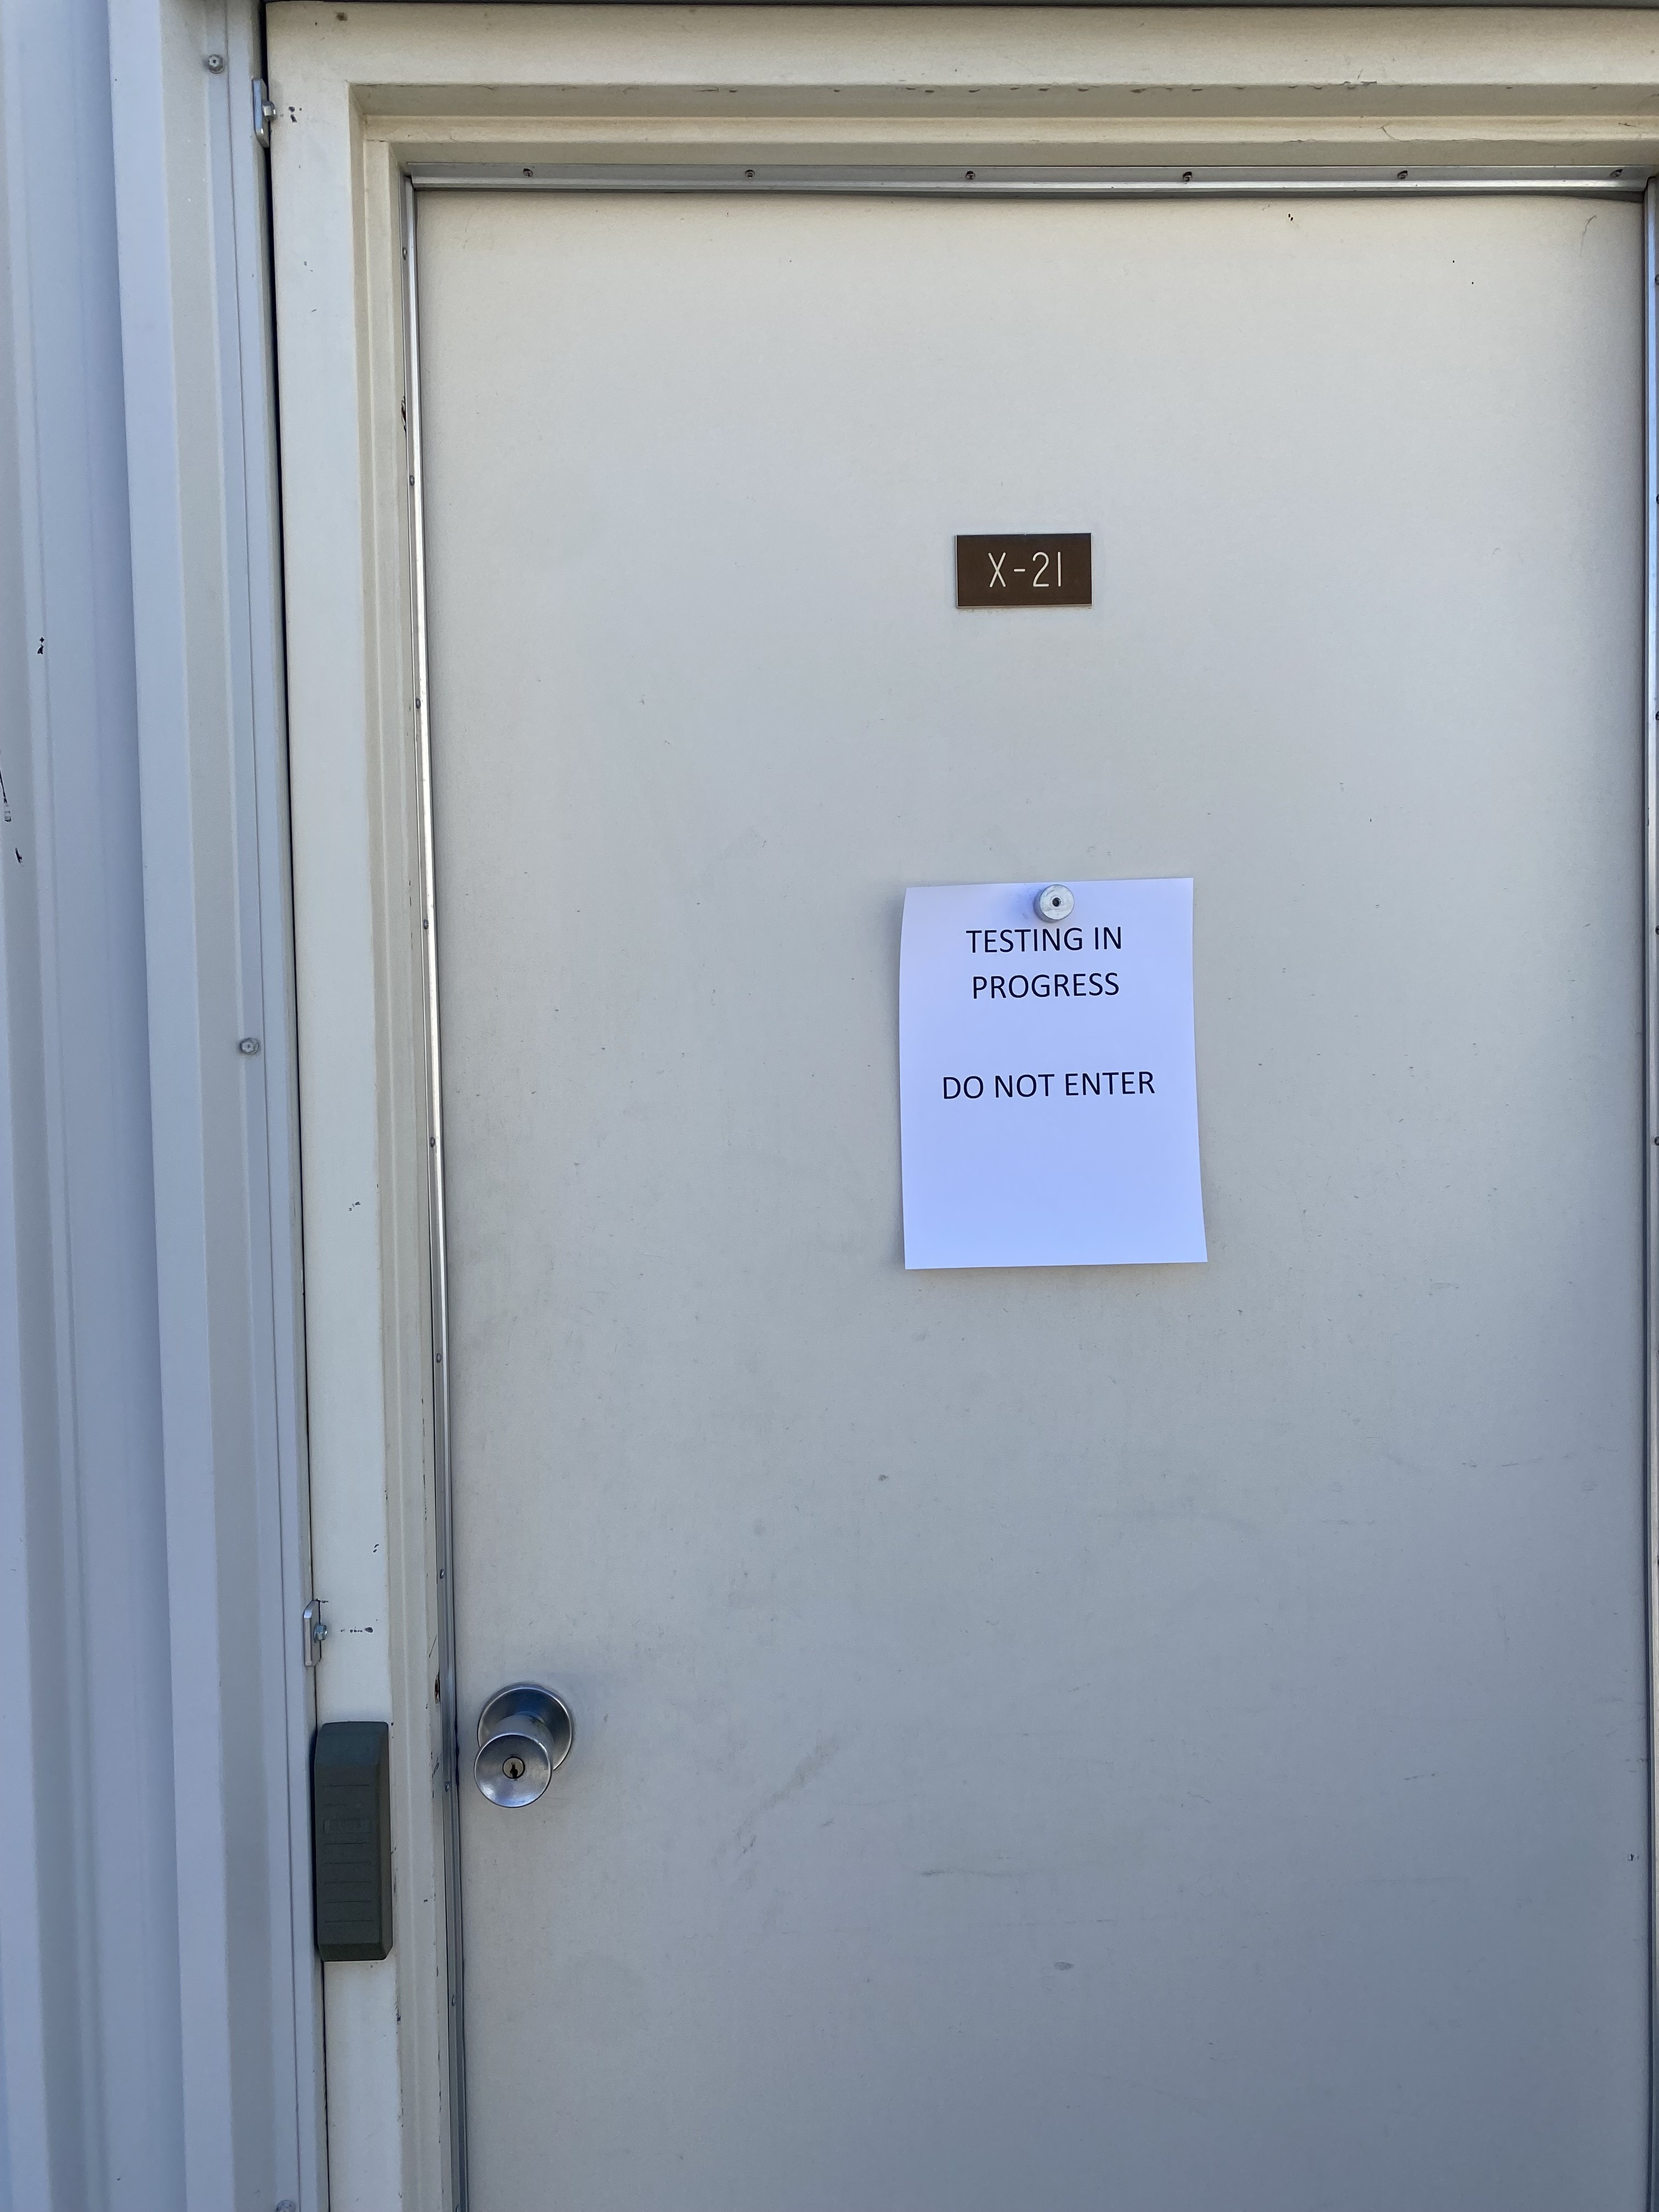
\includegraphics[width=3.12500in]{jira_imgs/3960.jpg}

}
\begin{tabular}{p{2cm}p{14cm}}
\toprule
Step 2 & Step Execution Status: \textbf{ Pass } \\ \hline
\end{tabular}
 Description \\
{\footnotesize
Verify the mechanical interfaces have been set up according to drawing
800-000.

}
\hdashrule[0.5ex]{\textwidth}{1pt}{3mm}
  Test Data \\
 {\footnotesize
\textbf{Note:~}This will initially be done with the aluminum surrogate
mass in place of the actuator.

}
\hdashrule[0.5ex]{\textwidth}{1pt}{3mm}
  Expected Result \\
{\footnotesize
The test bench is complete.

}
\hdashrule[0.5ex]{\textwidth}{1pt}{3mm}
  Actual Result \\
{\footnotesize
The test bench remained assembled from the unmodified actuator tests.

}
\begin{tabular}{p{2cm}p{14cm}}
\toprule
Step 3 & Step Execution Status: \textbf{ Pass } \\ \hline
\end{tabular}
 Description \\
{\footnotesize
Verify an air gauge is connected between the air supply and the air
valves.

}
\hdashrule[0.5ex]{\textwidth}{1pt}{3mm}
  Expected Result \\
{\footnotesize
\begin{itemize}
\tightlist
\item
  The air gauge is in position and capable of reading the psi value
  being supplied to the air valves.
\item
  The air gauge should initially show no air being supplied.
\end{itemize}

}
\hdashrule[0.5ex]{\textwidth}{1pt}{3mm}
  Actual Result \\
{\footnotesize
The test bench remained assembled from the unmodified actuator tests,
including the air gauges.

}
\begin{tabular}{p{2cm}p{14cm}}
\toprule
Step 4 & Step Execution Status: \textbf{ Pass } \\ \hline
\end{tabular}
 Description \\
{\footnotesize
Verify the valves for tension and compression are capable of displaying
commanded voltage.~

}
\hdashrule[0.5ex]{\textwidth}{1pt}{3mm}
  Expected Result \\
{\footnotesize
Both air gauges are in place monitoring the output from both the tension
and compression air valves.

}
\hdashrule[0.5ex]{\textwidth}{1pt}{3mm}
  Actual Result \\
{\footnotesize
The valves were validated to still be functional.~

}
\begin{tabular}{p{2cm}p{14cm}}
\toprule
Step 5 & Step Execution Status: \textbf{ Pass } \\ \hline
\end{tabular}
 Description \\
{\footnotesize
Make the connection between the two sets of air valves and gauges and
the USB-4716 readout device.\\
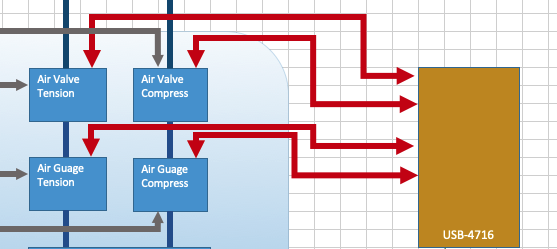
\includegraphics[width=3.12500in]{jira_imgs/3435.png}

}
\hdashrule[0.5ex]{\textwidth}{1pt}{3mm}
  Expected Result \\
{\footnotesize
The air valves and gauges are hooked up to the USB-4716 readout device.~

}
\hdashrule[0.5ex]{\textwidth}{1pt}{3mm}
  Actual Result \\
{\footnotesize
The test bench remained assembled from the unmodified actuator tests,
including the connections between the air valves and gauges to the
readout device.

}
\begin{tabular}{p{2cm}p{14cm}}
\toprule
Step 6 & Step Execution Status: \textbf{ Pass } \\ \hline
\end{tabular}
 Description \\
{\footnotesize
Make the connection between the MB5U readout electronics and the
renishaw encoders.

}
\hdashrule[0.5ex]{\textwidth}{1pt}{3mm}
  Expected Result \\
{\footnotesize
The MB5U readouts are connected to the encoders.

}
\hdashrule[0.5ex]{\textwidth}{1pt}{3mm}
  Actual Result \\
{\footnotesize
The encoder arms were re-installed with the modified actuator.

}
\begin{tabular}{p{2cm}p{14cm}}
\toprule
Step 7 & Step Execution Status: \textbf{ Pass } \\ \hline
\end{tabular}
 Description \\
{\footnotesize
Make the connection between the 9150 load cell readout electronic and
the load cell.

}
\hdashrule[0.5ex]{\textwidth}{1pt}{3mm}
  Expected Result \\
{\footnotesize
The load cell is connected to the load cell readout electronic.

}
\hdashrule[0.5ex]{\textwidth}{1pt}{3mm}
  Actual Result \\
{\footnotesize
The test bench remained assembled from the unmodified actuator tests,
including the Tovey reader and the load cell.

}
\begin{tabular}{p{2cm}p{14cm}}
\toprule
Step 8 & Step Execution Status: \textbf{ Pass } \\ \hline
\end{tabular}
 Description \\
{\footnotesize
Make the connection between the Hexapod Actuator to the thermal
scanner.~

}
\hdashrule[0.5ex]{\textwidth}{1pt}{3mm}
  Expected Result \\
{\footnotesize
The thermal scanner is connected to the hexapod actuator.

}
\hdashrule[0.5ex]{\textwidth}{1pt}{3mm}
  Actual Result \\
{\footnotesize
The thermal scanner was initially unavailable but was connected for the
Actuator Accelerated Life Test.

}
\begin{tabular}{p{2cm}p{14cm}}
\toprule
Step 9 & Step Execution Status: \textbf{ Pass } \\ \hline
\end{tabular}
 Description \\
{\footnotesize
Connect the following to the USB 3.0 Hub:

\begin{itemize}
\tightlist
\item
  (2) connections for MB5U Readout Electronic
\item
  USB-4716 Readout Device/Labjack T4
\item
  Temperature Readout
\item
  9150 Load Cell Readout Electronic
\end{itemize}

}
\hdashrule[0.5ex]{\textwidth}{1pt}{3mm}
  Expected Result \\
{\footnotesize
The USB 3.0 Hub is now connected to the readout electronics from the
previous steps.~

}
\hdashrule[0.5ex]{\textwidth}{1pt}{3mm}
  Actual Result \\
{\footnotesize
The test bench remained assembled from the unmodified actuator tests,
including the USB 3.0 Hub.

}
\begin{tabular}{p{2cm}p{14cm}}
\toprule
Step 10 & Step Execution Status: \textbf{ Pass } \\ \hline
\end{tabular}
 Description \\
{\footnotesize
Connect the laptop with LabVIEW software to the USB 3.0 Hub.

}
\hdashrule[0.5ex]{\textwidth}{1pt}{3mm}
  Expected Result \\
{\footnotesize
The Laptop is connected to the USB 3.0 Hub and to the subsequent readout
electronics.~

}
\hdashrule[0.5ex]{\textwidth}{1pt}{3mm}
  Actual Result \\
{\footnotesize
The laptop remained connected from the Unmodified Single Hexapod
Actuator Redesign Verification campaign.

}
\begin{tabular}{p{2cm}p{14cm}}
\toprule
Step 11 & Step Execution Status: \textbf{ Pass } \\ \hline
\end{tabular}
 Description \\
{\footnotesize
Connect the laptop to the Copley Motor drive of the Control Box.

}
\hdashrule[0.5ex]{\textwidth}{1pt}{3mm}
  Expected Result \\
{\footnotesize
The laptop is connected to the control box.

}
\hdashrule[0.5ex]{\textwidth}{1pt}{3mm}
  Actual Result \\
{\footnotesize
The copley motor drive remained connected from the Unmodified Single
Hexapod Actuator Redesign Verification campaign.

}
\begin{tabular}{p{2cm}p{14cm}}
\toprule
Step 12 & Step Execution Status: \textbf{ Pass } \\ \hline
\end{tabular}
 Description \\
{\footnotesize
Set up the USB 3.0 Hub close to the test fixture and connect it to a
power source.~

}
\hdashrule[0.5ex]{\textwidth}{1pt}{3mm}
  Expected Result \\
{\footnotesize
The USB 3.0 Hub is connected and all readout devices are powered on.~

}
\hdashrule[0.5ex]{\textwidth}{1pt}{3mm}
  Actual Result \\
{\footnotesize
The USB 3.0 Hub remained fixed to the test rig from the Unmodified
Single Hexapod Actuator Redesign Verification campaign.

}
\begin{tabular}{p{2cm}p{14cm}}
\toprule
Step 13 & Step Execution Status: \textbf{ Pass } \\ \hline
\end{tabular}
 Description \\
{\footnotesize
Verify that the output data from the readout devices are available on
the laptop.

}
\hdashrule[0.5ex]{\textwidth}{1pt}{3mm}
  Expected Result \\
{\footnotesize
The laptop is seen to be able to communicate with the readout devices.

}
\hdashrule[0.5ex]{\textwidth}{1pt}{3mm}
  Actual Result \\
{\footnotesize
The data was able to be read as expected.

}
\begin{tabular}{p{2cm}p{14cm}}
\toprule
Step 14 & Step Execution Status: \textbf{ Pass } \\ \hline
\end{tabular}
 Description \\
{\footnotesize
Open Labview 2021 in the computer used for Test Setup.

}
\hdashrule[0.5ex]{\textwidth}{1pt}{3mm}
  Expected Result \\
{\footnotesize
Labview 2021 opens successfully.

}
\hdashrule[0.5ex]{\textwidth}{1pt}{3mm}
  Actual Result \\
{\footnotesize
Labview was opened successfully.

}
\begin{tabular}{p{2cm}p{14cm}}
\toprule
Step 15 & Step Execution Status: \textbf{ Pass } \\ \hline
\end{tabular}
 Description \\
{\footnotesize
Open the Labview VI files from the project directory including sub VIs-
Tovey Closed loop.vi, Voltage Regulation.vi and Biss Reader.vi

}
\hdashrule[0.5ex]{\textwidth}{1pt}{3mm}
  Expected Result \\
{\footnotesize
Front panel of VI and sub VI files open without any error.

}
\hdashrule[0.5ex]{\textwidth}{1pt}{3mm}
  Actual Result \\
{\footnotesize
The VI's used for the test were opened successfully.

}
\begin{tabular}{p{2cm}p{14cm}}
\toprule
Step 16 & Step Execution Status: \textbf{ Pass } \\ \hline
\end{tabular}
 Description \\
{\footnotesize
Configure the Biss Reader.vi file with the appropriate configuration
file and following the IBISS operation manual.~

}
\hdashrule[0.5ex]{\textwidth}{1pt}{3mm}
  Expected Result \\
{\footnotesize
\href{https://jira.lsstcorp.org/rest/tests/1.0/attachment/3555}{BiSS\_config.cfg}
is loaded in the LabView configuration (Misc Tab under Load DLL). The
configuration file is based on the IBISS operation manual.

}
\hdashrule[0.5ex]{\textwidth}{1pt}{3mm}
  Actual Result \\
{\footnotesize
The Labview configuration was loaded successfully.

}
\begin{tabular}{p{2cm}p{14cm}}
\toprule
Step 17 & Step Execution Status: \textbf{ Pass } \\ \hline
\end{tabular}
 Description \\
{\footnotesize
Click Run button on the on the block diagram toolbar of the Labview VI
front panel.

}
\hdashrule[0.5ex]{\textwidth}{1pt}{3mm}
  Expected Result \\
{\footnotesize
LabView VI and ~associated sub Vi runs successfully. Initially all the
graphs and input values will be blank.

}
\hdashrule[0.5ex]{\textwidth}{1pt}{3mm}
  Actual Result \\
{\footnotesize
The LabView VI was able to be run without errors.

}
\begin{tabular}{p{2cm}p{14cm}}
\toprule
Step 18 & Step Execution Status: \textbf{ Pass } \\ \hline
\end{tabular}
 Description \\
{\footnotesize
Send a command through LabVIEW ~voltage Regulation.vi to set the voltage
on the compression valve only to 3V.

}
\hdashrule[0.5ex]{\textwidth}{1pt}{3mm}
  Expected Result \\
{\footnotesize
The command is accepted, the pneumatic valve shows the applied voltage
only on the compression valve and the applied compression force can be
seen on the LabView front panel Time vs Load graph.~

}
\hdashrule[0.5ex]{\textwidth}{1pt}{3mm}
  Actual Result \\
{\footnotesize
Using the LabView VI, we were able to adjust the voltage on the
pneumatic valves to 3V.

}
\begin{tabular}{p{2cm}p{14cm}}
\toprule
Step 19 & Step Execution Status: \textbf{ Pass } \\ \hline
\end{tabular}
 Description \\
{\footnotesize
Send a command through LabVIEW voltage Regulation.vi to reset the
compression valve to 0V.

}
\hdashrule[0.5ex]{\textwidth}{1pt}{3mm}
  Expected Result \\
{\footnotesize
The command is accepted. The applied force can be seen as zero load on
the LabView front panel Time vs Load graph. Load Cell Reader also shows
zero load.

}
\hdashrule[0.5ex]{\textwidth}{1pt}{3mm}
  Actual Result \\
{\footnotesize
The voltage was reset to 0V.

}
\begin{tabular}{p{2cm}p{14cm}}
\toprule
Step 20 & Step Execution Status: \textbf{ Pass } \\ \hline
\end{tabular}
 Description \\
{\footnotesize
Send a command through LabVIEW to reset the tension valve to 3V.

}
\hdashrule[0.5ex]{\textwidth}{1pt}{3mm}
  Expected Result \\
{\footnotesize
The command is accepted, the readout electronic shows the applied
voltage only on the tension valve and the applied tension force can be
seen on the LabView front panel Time vs Load graph.

}
\hdashrule[0.5ex]{\textwidth}{1pt}{3mm}
  Actual Result \\
{\footnotesize
Using the LabView VI, we were able to adjust the voltage on the
pneumatic valves to 3V.

}
\begin{tabular}{p{2cm}p{14cm}}
\toprule
Step 21 & Step Execution Status: \textbf{ Pass } \\ \hline
\end{tabular}
 Description \\
{\footnotesize
Send a command through LabVIEW to reset the tension valve to 0V.

}
\hdashrule[0.5ex]{\textwidth}{1pt}{3mm}
  Expected Result \\
{\footnotesize
The command is accepted, the readout electronic no longer shows the
applied voltage on the tension valve and there is no longer any tension
force on the LabView front panel Time vs Load graph.

}
\hdashrule[0.5ex]{\textwidth}{1pt}{3mm}
  Actual Result \\
{\footnotesize
The voltage was reset to 0V.

}
\begin{tabular}{p{2cm}p{14cm}}
\toprule
Step 22 & Step Execution Status: \textbf{ Pass } \\ \hline
\end{tabular}
 Description \\
{\footnotesize
Verify the laptop is reading the renishaw scales usinthe Biss Reader.vi
file and determine the zero stroke position.

}
\hdashrule[0.5ex]{\textwidth}{1pt}{3mm}
  Test Data \\
 {\footnotesize
\textbf{Note:~}Moog's original test procedure cited the zero position to
be at 40mm since the full length was 80mm.

}
\hdashrule[0.5ex]{\textwidth}{1pt}{3mm}
  Expected Result \\
{\footnotesize
40mm encoder readings shown in Labview front panel of the .vi file.~\\
The zero stroke position has been determined and can be used as a
reference for the offset of future moves.

}
\hdashrule[0.5ex]{\textwidth}{1pt}{3mm}
  Actual Result \\
{\footnotesize
The starting positions were seen as follows:

\begin{itemize}
\tightlist
\item
  Copley Software: Active Load Position = \textbf{-22.008mm or -22008750
  counts}
\item
  Encoder A (D13B) = 39.4mm
\item
  Encoder B (D0BD) = 39.5mm
\end{itemize}

Note: No load was applied during this step

}
\begin{tabular}{p{2cm}p{14cm}}
\toprule
Step 23 & Step Execution Status: \textbf{ Pass } \\ \hline
\end{tabular}
 Description \\
{\footnotesize
Using the Copley Software, drive the actuator to the positive limit
switch and take note of the values measured by the Copley Software and
the Encoder Readings.

}
\hdashrule[0.5ex]{\textwidth}{1pt}{3mm}
  Expected Result \\
{\footnotesize
The actuator is able to hit the positive limit switch and the values are
recorded.

}
\hdashrule[0.5ex]{\textwidth}{1pt}{3mm}
  Actual Result \\
{\footnotesize
The positive limit switch was initially reached reading the following
values:

\begin{itemize}
\tightlist
\item
  Copley Software: Active Load Position = \textbf{-8.5mm or
  -8547035counts}
\item
  Encoder A (D13B) = 25.88mm
\item
  Encoder B (D0BD) = 26.17mm
\end{itemize}

Note: No load was applied during this step\\[2\baselineskip]However, the
positive limit switch was adjusted to:\\

\begin{itemize}
\tightlist
\item
  Copley Software: Active Load Position = \textbf{-7.515mm or
  -7515000counts}
\item
  Encoder A (D13B) = 24.78mm
\item
  Encoder B (D0BD) = 25.23mm
\end{itemize}

}
\begin{tabular}{p{2cm}p{14cm}}
\toprule
Step 24 & Step Execution Status: \textbf{ Pass } \\ \hline
\end{tabular}
 Description \\
{\footnotesize
Using the Copley Software, drive the actuator to the negative limit
switch and take note of the values measured by the Copley Software and
the Encoder Readings.

}
\hdashrule[0.5ex]{\textwidth}{1pt}{3mm}
  Expected Result \\
{\footnotesize
The actuator is able to hit the negative limit switch and the values are
recorded.

}
\hdashrule[0.5ex]{\textwidth}{1pt}{3mm}
  Actual Result \\
{\footnotesize
Moving in the negative direction, the negative limit was triggered
at\textbf{~-33.81mm or -33810000 counts}\\
The starting linear encoder position was 39mm and
XYmm\\[2\baselineskip]The negative limit switch was reached reading the
following values:

\begin{itemize}
\tightlist
\item
  Copley Software: Active Load Position = -\textbf{33.81mm or -33810000
  counts}
\item
  Encoder A (D13B) = 51.17mm
\item
  Encoder B (D0BD) = 51.45mm
\end{itemize}

Note: No load was applied during this step\\[2\baselineskip]However, the
negative limit switch was adjusted to:\\

\begin{itemize}
\tightlist
\item
  Copley Software: Active Load Position = \textbf{-36.03mm or
  -36003000counts}
\item
  Encoder A (D13B) = 53.28mm
\item
  Encoder B (D0BD) = 53.73
\end{itemize}

}

\paragraph{ LVV-T2426 - Hexapod - Actuator Proofing Testing with 200\% load }\mbox{}\\

Version \textbf{1}.
Status \textbf{Approved}.
Open  \href{https://jira.lsstcorp.org/secure/Tests.jspa#/testCase/LVV-T2426}{\textit{ LVV-T2426 } }
test case in Jira.

To perform the actuator proofing test with 200\% load in order to verify
the \citeds{LTS-206} hexapod proof testing requirement.~

\textbf{ Preconditions}:\\


Execution status: {\bf Pass }

Final comment:\\In order to prevent over stressing the actuator, this test was only
conducted on the modified actuator. During this test, there were no
obvious signs of damage so this test was considered passed. The data
taken from this test case be seen in the attached \emph{200\% Proofing
Test Results - Modified Actuator.xlsx}.


Detailed steps results:

\begin{tabular}{p{2cm}p{14cm}}
\toprule
Step 1 & Step Execution Status: \textbf{ Pass } \\ \hline
\end{tabular}
 Description \\
{\footnotesize
Open Labview 2021 in the computer used for Test Setup.

}
\hdashrule[0.5ex]{\textwidth}{1pt}{3mm}
  Test Data \\
 {\footnotesize
\textbf{Note:~}The first three steps are conditional because these steps
are included as part of the Test Setup procedure and may not be
necessary if LabView is still open.

}
\hdashrule[0.5ex]{\textwidth}{1pt}{3mm}
  Expected Result \\
{\footnotesize
Labview 2021 opens successfully.

}
\hdashrule[0.5ex]{\textwidth}{1pt}{3mm}
  Actual Result \\
{\footnotesize
Labview was opened successfully.

}
\begin{tabular}{p{2cm}p{14cm}}
\toprule
Step 2 & Step Execution Status: \textbf{ Pass } \\ \hline
\end{tabular}
 Description \\
{\footnotesize
Run the following VI's:

\begin{itemize}
\tightlist
\item
  Encoder A (D13B) and Load Cell.vi
\item
  Encoder B (D0BD).vi
\end{itemize}

}
\hdashrule[0.5ex]{\textwidth}{1pt}{3mm}
  Expected Result \\
{\footnotesize
Front panel of VI's open without any error.

}
\hdashrule[0.5ex]{\textwidth}{1pt}{3mm}
  Actual Result \\
{\footnotesize
The VI's were opened with no issue.

}
\begin{tabular}{p{2cm}p{14cm}}
\toprule
Step 3 & Step Execution Status: \textbf{ Pass } \\ \hline
\end{tabular}
 Description \\
{\footnotesize
Click Run button on the on the block diagram toolbar of the Labview VI
front panel.

}
\hdashrule[0.5ex]{\textwidth}{1pt}{3mm}
  Expected Result \\
{\footnotesize
LabView VI and associated sub Vi runs successfully. The graphs should
start to be populated with data once the run button is pressed.

}
\hdashrule[0.5ex]{\textwidth}{1pt}{3mm}
  Actual Result \\
{\footnotesize
The VI's were able to run.

}
\begin{tabular}{p{2cm}p{14cm}}
\toprule
Step 4 & Step Execution Status: \textbf{ Pass } \\ \hline
\end{tabular}
 Description \\
{\footnotesize
Position the actuator at its center of stroke position using the control
box and copley software.~

}
\hdashrule[0.5ex]{\textwidth}{1pt}{3mm}
  Expected Result \\
{\footnotesize
Actuator positioned at its center of stroke position ~confirmed by
encoder reading in the LabView.

}
\hdashrule[0.5ex]{\textwidth}{1pt}{3mm}
  Actual Result \\
{\footnotesize
The actuator is in its ``zero position''\\

\begin{itemize}
\tightlist
\item
  Copley Software: Active Load Position = \textbf{-22.00mm}
\item
  Encoder A (D13B) = 39.29mm
\item
  Encoder B (D0BD) = 39.73mm
\end{itemize}

}
\begin{tabular}{p{2cm}p{14cm}}
\toprule
Step 5 & Step Execution Status: \textbf{ Pass } \\ \hline
\end{tabular}
 Description \\
{\footnotesize
Disable Motor Power by pressing the Emergency stop button on the control
box.

}
\hdashrule[0.5ex]{\textwidth}{1pt}{3mm}
  Expected Result \\
{\footnotesize
Motor power disabled.~

}
\hdashrule[0.5ex]{\textwidth}{1pt}{3mm}
  Actual Result \\
{\footnotesize
Control software confirms the Amp Hardware is Disabled

}
\begin{tabular}{p{2cm}p{14cm}}
\toprule
Step 6 & Step Execution Status: \textbf{ Pass } \\ \hline
\end{tabular}
 Description \\
{\footnotesize
Slowly apply an increasing tension force with the load actuator until a
force of 60 kN (13,489 lbf) through the Encoder A (D13B) and Load
Cell.vi

}
\hdashrule[0.5ex]{\textwidth}{1pt}{3mm}
  Test Data \\
 {\footnotesize
\textbf{Note:~}Set valve to 8.76V to apply a +/-60kN force.

}
\hdashrule[0.5ex]{\textwidth}{1pt}{3mm}
  Expected Result \\
{\footnotesize
Tension force applied to the actuator increasingly.

}
\hdashrule[0.5ex]{\textwidth}{1pt}{3mm}
  Actual Result \\
{\footnotesize
Gradually applied the force in tension starting at 20kN, then 30kN,
40kN, 50kN, 55kN, 56kN, 57kN, 58kN, 59kN and finally 60kN. 60kN of
tension was achieved by applying 9.15V on the tension valve (channel 1).

}
\begin{tabular}{p{2cm}p{14cm}}
\toprule
Step 7 & Step Execution Status: \textbf{ Pass } \\ \hline
\end{tabular}
 Description \\
{\footnotesize
Make sure the load does not go over 60 kN, as this load represents the
2X the max load or proof test load case.~

}
\hdashrule[0.5ex]{\textwidth}{1pt}{3mm}
  Expected Result \\
{\footnotesize
In the LabView load graph and load cell reader, showing the 60 KN
tension force.

}
\hdashrule[0.5ex]{\textwidth}{1pt}{3mm}
  Actual Result \\
{\footnotesize
60kN of tension is applied.

}
\begin{tabular}{p{2cm}p{14cm}}
\toprule
Step 8 & Step Execution Status: \textbf{ Pass } \\ \hline
\end{tabular}
 Description \\
{\footnotesize
Continue to apply the load for 10 minutes and observe for any unexpected
movement or sounds. Check for the Encoder Readings in the Time vs
Displacement graphs on the Labview BISS Reader VI for 10 minutes.~

}
\hdashrule[0.5ex]{\textwidth}{1pt}{3mm}
  Test Data \\
 {\footnotesize
\textbf{Note:~}Maintain the force on the cell by keeping the same
voltage in the LabView voltage regulation VI.

}
\hdashrule[0.5ex]{\textwidth}{1pt}{3mm}
  Expected Result \\
{\footnotesize
No unexpected movement or sounds recorded to indicate any catastrophic
failure.

}
\hdashrule[0.5ex]{\textwidth}{1pt}{3mm}
  Actual Result \\
{\footnotesize
The 60kN tension load was applied at 3:58pm and kept on until 4:08pm.

}
\begin{tabular}{p{2cm}p{14cm}}
\toprule
Step 9 & Step Execution Status: \textbf{ Pass } \\ \hline
\end{tabular}
 Description \\
{\footnotesize
Slowly remove the tension force to return to zero load.~

}
\hdashrule[0.5ex]{\textwidth}{1pt}{3mm}
  Expected Result \\
{\footnotesize
Tension force removed and load cell reading in the lab-view graph and
load cell reader showing zero load.

}
\hdashrule[0.5ex]{\textwidth}{1pt}{3mm}
  Actual Result \\
{\footnotesize
The load was gradually released.~

}
\begin{tabular}{p{2cm}p{14cm}}
\toprule
Step 10 & Step Execution Status: \textbf{ Pass } \\ \hline
\end{tabular}
 Description \\
{\footnotesize
Return the position the actuator to its center of stroke position using
the control box and copley software..

}
\hdashrule[0.5ex]{\textwidth}{1pt}{3mm}
  Test Data \\
 {\footnotesize
\textbf{Note:~}This is where the linear encoder reads 40mm.~

}
\hdashrule[0.5ex]{\textwidth}{1pt}{3mm}
  Expected Result \\
{\footnotesize
Actuator positioned at its center of stroke position ~confirmed by
encoder reading in the LabView.

}
\hdashrule[0.5ex]{\textwidth}{1pt}{3mm}
  Actual Result \\
{\footnotesize
By the end of the 10 minutes, the final positions were seen to be:\\

\begin{itemize}
\tightlist
\item
  Copley Software: Active Load Position = \textbf{-22.34mm}
\item
  Encoder A (D13B) = 40.00mm
\item
  Encoder B (D0BD) = 40.43mm
\end{itemize}

Once the load was removed, the positions were:\\

\begin{itemize}
\tightlist
\item
  Copley Software: Active Load Position = \textbf{-21.99mm}
\item
  Encoder A (D13B) = 39.35mm
\item
  Encoder B (D0BD) = 39.77mm
\end{itemize}

}
\begin{tabular}{p{2cm}p{14cm}}
\toprule
Step 11 & Step Execution Status: \textbf{ Pass } \\ \hline
\end{tabular}
 Description \\
{\footnotesize
Slowly apply an increasing compression force with the load actuator
until a force of 60 kN (13,489 lbf) is reached using Lab view Vi
regulator.~

}
\hdashrule[0.5ex]{\textwidth}{1pt}{3mm}
  Test Data \\
 {\footnotesize
\textbf{Note:~}Set valve to 8.76V to apply a +/-60kN force.

}
\hdashrule[0.5ex]{\textwidth}{1pt}{3mm}
  Expected Result \\
{\footnotesize
Load graph and Load Cell Reader showing 60 kN compression force applied
to the actuator increasingly.

}
\hdashrule[0.5ex]{\textwidth}{1pt}{3mm}
  Actual Result \\
{\footnotesize
Gradually applied the force in tension starting at -20kN, then -30kN,
-40kN, -50kN, -55kN, -56kN, -57kN, -58kN, -59kN and finally -60kN.\\
Note: -60kN of tension was achieved by applying 8.82V on the compression
valve (channel 0).

}
\begin{tabular}{p{2cm}p{14cm}}
\toprule
Step 12 & Step Execution Status: \textbf{ Pass } \\ \hline
\end{tabular}
 Description \\
{\footnotesize
Make sure the load does not go over 60 kN ~as this load represents the
2X the max load or proof test load case.

}
\hdashrule[0.5ex]{\textwidth}{1pt}{3mm}
  Expected Result \\
{\footnotesize
In the LabView load graph,load does not surpass 60 kN.

}
\hdashrule[0.5ex]{\textwidth}{1pt}{3mm}
  Actual Result \\
{\footnotesize
-60.2kN of compression was applied

}
\begin{tabular}{p{2cm}p{14cm}}
\toprule
Step 13 & Step Execution Status: \textbf{ Pass } \\ \hline
\end{tabular}
 Description \\
{\footnotesize
Continue to apply the load for 10 minutes and observe for any unexpected
movement or sounds.

}
\hdashrule[0.5ex]{\textwidth}{1pt}{3mm}
  Expected Result \\
{\footnotesize
\textbf{No unexpected movement or sounds recorded to indicate any
catastrophic failure.}

}
\hdashrule[0.5ex]{\textwidth}{1pt}{3mm}
  Actual Result \\
{\footnotesize
The -60kN compression load was applied at 4:15pm and kept on until
4:25pm.

}
\begin{tabular}{p{2cm}p{14cm}}
\toprule
Step 14 & Step Execution Status: \textbf{ Pass } \\ \hline
\end{tabular}
 Description \\
{\footnotesize
Slowly remove the compression force to return to the zero load.

}
\hdashrule[0.5ex]{\textwidth}{1pt}{3mm}
  Expected Result \\
{\footnotesize
Compression force removed and load cell reading in the lab-view graph
and load cell reader showing zero load.

}
\hdashrule[0.5ex]{\textwidth}{1pt}{3mm}
  Actual Result \\
{\footnotesize
By the end of the 10 minutes, the final positions were seen to be:\\

\begin{itemize}
\tightlist
\item
  Copley Software: Active Load Position = \textbf{-22.34mm}
\item
  Encoder A (D13B) = 38.73mm
\item
  Encoder B (D0BD) = 39.39mm
\end{itemize}

Once the load was removed, the positions were:\\

\begin{itemize}
\tightlist
\item
  Copley Software: Active Load Position = \textbf{-21.95mm}
\item
  Encoder A (D13B) = 39.24mm
\item
  Encoder B (D0BD) = 39.71mm
\end{itemize}

}
\begin{tabular}{p{2cm}p{14cm}}
\toprule
Step 15 & Step Execution Status: \textbf{ Pass } \\ \hline
\end{tabular}
 Description \\
{\footnotesize
Press Stop button in the VI file front panel to stop reading of the
components

}
\hdashrule[0.5ex]{\textwidth}{1pt}{3mm}
  Expected Result \\
{\footnotesize
Graphs in the front panel of the VI file becomes static.

}
\hdashrule[0.5ex]{\textwidth}{1pt}{3mm}
  Actual Result \\
{\footnotesize
The vi is stopped.

}
\begin{tabular}{p{2cm}p{14cm}}
\toprule
Step 16 & Step Execution Status: \textbf{ Pass } \\ \hline
\end{tabular}
 Description \\
{\footnotesize
Check if all the test results are recorded in excel spreadsheets.

}
\hdashrule[0.5ex]{\textwidth}{1pt}{3mm}
  Expected Result \\
{\footnotesize
Test Results are recorded in the excel spreadsheets residing in the
LabView Folder directory.

}
\hdashrule[0.5ex]{\textwidth}{1pt}{3mm}
  Actual Result \\
{\footnotesize
Data saved into the attached excel sheets.

}
\begin{tabular}{p{2cm}p{14cm}}
\toprule
Step 17 & Step Execution Status: \textbf{ Not Executed } \\ \hline
\end{tabular}
 Description \\
{\footnotesize
Close all the Labview VI files.

}
\hdashrule[0.5ex]{\textwidth}{1pt}{3mm}
  Test Data \\
 {\footnotesize
\textbf{Note:} Labview can be left open in order to continue to the next
test. However, it may be necessary to reset the application before
starting the next test.

}
\hdashrule[0.5ex]{\textwidth}{1pt}{3mm}
  Expected Result \\
{\footnotesize
All the VI files are closed and Labview 2021 application window closes.

}
\hdashrule[0.5ex]{\textwidth}{1pt}{3mm}
  Actual Result \\
{\footnotesize
The VI's were kept open in order to continue with the next test

}

\paragraph{ LVV-T2427 - Hexapod - Actuator Back Driving Test }\mbox{}\\

Version \textbf{1}.
Status \textbf{Approved}.
Open  \href{https://jira.lsstcorp.org/secure/Tests.jspa#/testCase/LVV-T2427}{\textit{ LVV-T2427 } }
test case in Jira.

The objective of this test case is to verify that removing the power
from an actuator will not cause the actuator to back drive even with the
application of different loads.

\textbf{ Preconditions}:\\
Proofing 200\% load test should be performed before running the
back-driving test.~

Execution status: {\bf Pass }

Final comment:\\During the Unmodified Actuator Verification campaign, the internal
rotary encoder reading was not recorded and so the displacement as
measured by the external linear encoders were recorded instead. However,
during this Modified Actuator Verification campaign, the back driving
test was able to be conducted using the readings from the internal
rotary encoder. As a result, it can be seen in the steps below that the
back driving measured during this test was measured to be under 10
counts for both tension and compression load. The data as measured by
the external linear encoders can be seen in the attached \emph{Back
Drive Test Results - Unmodified Actuator (1).xlsm} excel file.


Detailed steps results:

\begin{tabular}{p{2cm}p{14cm}}
\toprule
Step 1.1 & Step Execution Status: \textbf{ Pass } \\ \hline
\end{tabular}
 Description \\
{\footnotesize
Open Labview 2021 in the computer used for Test Setup.

}
\hdashrule[0.5ex]{\textwidth}{1pt}{3mm}
  Test Data \\
 {\footnotesize
\textbf{Note:~}The first three steps are conditional because these steps
are included as part of the Test Setup procedure and may not be
necessary if LabView is still open.

}
\hdashrule[0.5ex]{\textwidth}{1pt}{3mm}
  Expected Result \\
{\footnotesize
Labview 2021 opens successfully.

}
\hdashrule[0.5ex]{\textwidth}{1pt}{3mm}
  Actual Result \\
{\footnotesize
Labview was already open from the previous test.

}
\begin{tabular}{p{2cm}p{14cm}}
\toprule
Step 1.2 & Step Execution Status: \textbf{ Pass } \\ \hline
\end{tabular}
 Description \\
{\footnotesize
Run the following VI's:

\begin{itemize}
\tightlist
\item
  Encoder A (D13B) and Load Cell.vi
\item
  Encoder B (D0BD).vi
\end{itemize}

}
\hdashrule[0.5ex]{\textwidth}{1pt}{3mm}
  Test Data \\
 {\footnotesize
\textbf{Note:~}Each vi is responsible for reading one encoder.

}
\hdashrule[0.5ex]{\textwidth}{1pt}{3mm}
  Expected Result \\
{\footnotesize
Front panel of VI's open without any error.

}
\hdashrule[0.5ex]{\textwidth}{1pt}{3mm}
  Actual Result \\
{\footnotesize
Labview was already open from the previous test.

}
\begin{tabular}{p{2cm}p{14cm}}
\toprule
Step 1.3 & Step Execution Status: \textbf{ Pass } \\ \hline
\end{tabular}
 Description \\
{\footnotesize
Click Run button on the block diagram toolbar of the Labview VI front
panel.

}
\hdashrule[0.5ex]{\textwidth}{1pt}{3mm}
  Expected Result \\
{\footnotesize
LabView VI and associated sub Vi runs successfully. The graphs should
start to be populated with data once the run button is pressed.

}
\hdashrule[0.5ex]{\textwidth}{1pt}{3mm}
  Actual Result \\
{\footnotesize
The VI was run again.

}
\begin{tabular}{p{2cm}p{14cm}}
\toprule
Step 1.4 & Step Execution Status: \textbf{ Pass } \\ \hline
\end{tabular}
 Description \\
{\footnotesize
Record the starting position of the actuator using the external
encoders.

}
\hdashrule[0.5ex]{\textwidth}{1pt}{3mm}
  Test Data \\
 {\footnotesize
\textbf{Note:~}The Copley software will display a value based on the
reading from its internal encoder, which may be useful to take note of.
However, the readings reported by the external encoders will validate
the reading of the internal encoder.

}
\hdashrule[0.5ex]{\textwidth}{1pt}{3mm}
  Expected Result \\
{\footnotesize
The actuator position is determined by the external encoders.

}
\hdashrule[0.5ex]{\textwidth}{1pt}{3mm}
  Actual Result \\
{\footnotesize
The actuator is in its ``zero position''\\

\begin{itemize}
\tightlist
\item
  Copley Software: Active Load Position = \textbf{-22.00mm}
\item
  Encoder A (D13B) = 39.29mm
\item
  Encoder B (D0BD) = 39.74mm
\end{itemize}

}
\begin{tabular}{p{2cm}p{14cm}}
\toprule
Step 1.5 & Step Execution Status: \textbf{ Pass } \\ \hline
\end{tabular}
 Description \\
{\footnotesize
Make sure motor drive is disabled using Copley software and the control
box.~

}
\hdashrule[0.5ex]{\textwidth}{1pt}{3mm}
  Expected Result \\
{\footnotesize
Motor drive is disabled.~

}
\hdashrule[0.5ex]{\textwidth}{1pt}{3mm}
  Actual Result \\
{\footnotesize
The E-Stop on the control box was pressed to disable the motor drive.

}
\begin{tabular}{p{2cm}p{14cm}}
\toprule
Step 1.6 & Step Execution Status: \textbf{ Pass } \\ \hline
\end{tabular}
 Description \\
{\footnotesize
Slowly apply an increasing {Tension}⁠ ~force of +/-37.5kN.~

}
\hdashrule[0.5ex]{\textwidth}{1pt}{3mm}
  Test Data \\
 {\footnotesize
\textbf{Note:~}Set the {Tension}⁠ valve to 5.48V in order to apply
+/-37.5kN of force.

}
\hdashrule[0.5ex]{\textwidth}{1pt}{3mm}
  Expected Result \\
{\footnotesize
Load cell reader shows the applied +/-37.5kN {Tension}⁠~ force.\\
LabView displays the voltage being applied.

}
\hdashrule[0.5ex]{\textwidth}{1pt}{3mm}
  Actual Result \\
{\footnotesize
+37.5kN was applied by setting channel 1 to 5.7V

}
\begin{tabular}{p{2cm}p{14cm}}
\toprule
Step 1.7 & Step Execution Status: \textbf{ Pass } \\ \hline
\end{tabular}
 Description \\
{\footnotesize
Record the displacement of the actuator using the external encoder
readings and verify the position as measured by the Copley software has
not changed significantly.

}
\hdashrule[0.5ex]{\textwidth}{1pt}{3mm}
  Expected Result \\
{\footnotesize
The final position of the actuator has been determined.\\
If the actuator position has changed significantly (\textgreater{}10
counts or 0.36 deg of motor rotation), the actuator has back-driven.

}
\hdashrule[0.5ex]{\textwidth}{1pt}{3mm}
  Actual Result \\
{\footnotesize
The data from the external linear encoders was exported into excel
sheets.\\
A screenshot was taken of the displacement as measured by the Copley
control software:\\
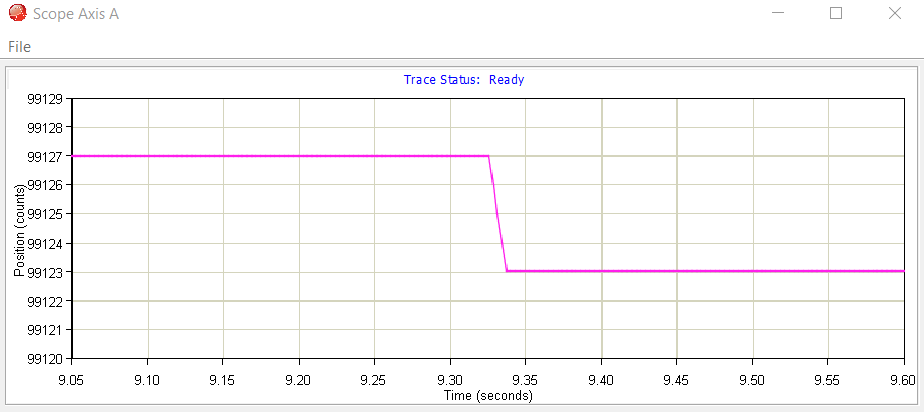
\includegraphics[width=5.90625in]{jira_imgs/3962.png}As seen in the
screenshot, the displacement after the tension load was applied was
about 4 counts.

}
\begin{tabular}{p{2cm}p{14cm}}
\toprule
Step 1.8 & Step Execution Status: \textbf{ Pass } \\ \hline
\end{tabular}
 Description \\
{\footnotesize
Confirm that there are no other signs of gross actuator motion.

}
\hdashrule[0.5ex]{\textwidth}{1pt}{3mm}
  Expected Result \\
{\footnotesize
No visual movement, significant motion of the internal linear encoder or
external linear test encoders beyond expected actuator compliance
recorded in the LabView displacement graphs.~

}
\hdashrule[0.5ex]{\textwidth}{1pt}{3mm}
  Actual Result \\
{\footnotesize
No visual signs of movement

}
\begin{tabular}{p{2cm}p{14cm}}
\toprule
Step 1.9 & Step Execution Status: \textbf{ Pass } \\ \hline
\end{tabular}
 Description \\
{\footnotesize
Reduce the {Tension}⁠ ~force to back to zero load.

}
\hdashrule[0.5ex]{\textwidth}{1pt}{3mm}
  Test Data \\
 {\footnotesize
\textbf{Note:~}In order to reset the load to zero, both the valves
should be set to 0V.

}
\hdashrule[0.5ex]{\textwidth}{1pt}{3mm}
  Expected Result \\
{\footnotesize
{Tension}⁠~ force removed and load cell reading in the lab-view graph
and load cell reader showing zero load.

}
\hdashrule[0.5ex]{\textwidth}{1pt}{3mm}
  Actual Result \\
{\footnotesize
Tension load was removed.

}
\begin{tabular}{p{2cm}p{14cm}}
\toprule
Step 2.0 & Step Execution Status: \textbf{ Pass } \\ \hline
\end{tabular}
 Description \\
{\footnotesize
Record the displacement of the actuator using the external encoder
readings.

}
\hdashrule[0.5ex]{\textwidth}{1pt}{3mm}
  Test Data \\
 {\footnotesize
\textbf{Note:~}The Copley software will display a value based on the
reading from its internal encoder, which may be useful to take note of.
However, the readings reported by the external encoders will validate
the reading of the internal encoder.

}
\hdashrule[0.5ex]{\textwidth}{1pt}{3mm}
  Expected Result \\
{\footnotesize
The final position of the actuator has been determined.\\
If the actuator position has changed significantly (\textgreater{}10
counts or 0.36 deg of motor rotation), the actuator has back-driven.

}
\hdashrule[0.5ex]{\textwidth}{1pt}{3mm}
  Actual Result \\
{\footnotesize
The actuator returns to its ``zero position''\\

\begin{itemize}
\tightlist
\item
  Copley Software: Active Load Position = \textbf{-22.00mm}
\item
  Encoder A (D13B) = 39.36mm
\item
  Encoder B (D0BD) = 39.78mm
\end{itemize}

}
\begin{tabular}{p{2cm}p{14cm}}
\toprule
Step 2.1 & Step Execution Status: \textbf{ Pass } \\ \hline
\end{tabular}
 Description \\
{\footnotesize
Check if all the test results are recorded in excel spreadsheets.

}
\hdashrule[0.5ex]{\textwidth}{1pt}{3mm}
  Test Data \\
 {\footnotesize


}
\hdashrule[0.5ex]{\textwidth}{1pt}{3mm}
  Expected Result \\
{\footnotesize
Test Results are recorded in the excel spreadsheets residing in the
LabView Folder directory.

}
\hdashrule[0.5ex]{\textwidth}{1pt}{3mm}
  Actual Result \\
{\footnotesize
The screenshot of the Copley Control Software can be seen in Step 7. The
data as recorded by the external linear encoders be seen in
the\emph{~Back Drive Test Results - Unmodified Actuator (1).xlsm} excel
file.

}
\begin{tabular}{p{2cm}p{14cm}}
\toprule
Step 2.1 & Step Execution Status: \textbf{ Pass } \\ \hline
\end{tabular}
 Description \\
{\footnotesize
Open Labview 2021 in the computer used for Test Setup.

}
\hdashrule[0.5ex]{\textwidth}{1pt}{3mm}
  Test Data \\
 {\footnotesize
\textbf{Note:~}The first three steps are conditional because these steps
are included as part of the Test Setup procedure and may not be
necessary if LabView is still open.

}
\hdashrule[0.5ex]{\textwidth}{1pt}{3mm}
  Expected Result \\
{\footnotesize
Labview 2021 opens successfully.

}
\hdashrule[0.5ex]{\textwidth}{1pt}{3mm}
  Actual Result \\
{\footnotesize
Labview was already open from the previous test.

}
\begin{tabular}{p{2cm}p{14cm}}
\toprule
Step 2.2 & Step Execution Status: \textbf{ Not Executed } \\ \hline
\end{tabular}
 Description \\
{\footnotesize
Close all the Labview VI files.

}
\hdashrule[0.5ex]{\textwidth}{1pt}{3mm}
  Test Data \\
 {\footnotesize
\textbf{Note:~}Labview can be left open in order to continue to the next
test. However, it may be necessary to reset the application before
starting the next test.

}
\hdashrule[0.5ex]{\textwidth}{1pt}{3mm}
  Expected Result \\
{\footnotesize
All the VI files are closed and Labview 2021 application window closes.

}
\hdashrule[0.5ex]{\textwidth}{1pt}{3mm}
  Actual Result \\
{\footnotesize
LabView was kept open to continue the next test.~

}
\begin{tabular}{p{2cm}p{14cm}}
\toprule
Step 2.2 & Step Execution Status: \textbf{ Pass } \\ \hline
\end{tabular}
 Description \\
{\footnotesize
Run the following VI's:

\begin{itemize}
\tightlist
\item
  Encoder A (D13B) and Load Cell.vi
\item
  Encoder B (D0BD).vi
\end{itemize}

}
\hdashrule[0.5ex]{\textwidth}{1pt}{3mm}
  Test Data \\
 {\footnotesize
\textbf{Note:~}Each vi is responsible for reading one encoder.

}
\hdashrule[0.5ex]{\textwidth}{1pt}{3mm}
  Expected Result \\
{\footnotesize
Front panel of VI's open without any error.

}
\hdashrule[0.5ex]{\textwidth}{1pt}{3mm}
  Actual Result \\
{\footnotesize
Labview was already open from the previous test.

}
\begin{tabular}{p{2cm}p{14cm}}
\toprule
Step 2.3 & Step Execution Status: \textbf{ Pass } \\ \hline
\end{tabular}
 Description \\
{\footnotesize
Click Run button on the block diagram toolbar of the Labview VI front
panel.

}
\hdashrule[0.5ex]{\textwidth}{1pt}{3mm}
  Expected Result \\
{\footnotesize
LabView VI and associated sub Vi runs successfully. The graphs should
start to be populated with data once the run button is pressed.

}
\hdashrule[0.5ex]{\textwidth}{1pt}{3mm}
  Actual Result \\
{\footnotesize
The VI was run again.

}
\begin{tabular}{p{2cm}p{14cm}}
\toprule
Step 2.4 & Step Execution Status: \textbf{ Pass } \\ \hline
\end{tabular}
 Description \\
{\footnotesize
Record the starting position of the actuator using the external
encoders.

}
\hdashrule[0.5ex]{\textwidth}{1pt}{3mm}
  Test Data \\
 {\footnotesize
\textbf{Note:~}The Copley software will display a value based on the
reading from its internal encoder, which may be useful to take note of.
However, the readings reported by the external encoders will validate
the reading of the internal encoder.

}
\hdashrule[0.5ex]{\textwidth}{1pt}{3mm}
  Expected Result \\
{\footnotesize
The actuator position is determined by the external encoders.

}
\hdashrule[0.5ex]{\textwidth}{1pt}{3mm}
  Actual Result \\
{\footnotesize
The actuator is in its ``zero position''\\

\begin{itemize}
\tightlist
\item
  Copley Software: Active Load Position = \textbf{-22.00mm}
\item
  Encoder A (D13B) = 39.17mm
\item
  Encoder B (D0BD) = 40.16mm
\end{itemize}

}
\begin{tabular}{p{2cm}p{14cm}}
\toprule
Step 2.5 & Step Execution Status: \textbf{ Pass } \\ \hline
\end{tabular}
 Description \\
{\footnotesize
Make sure motor drive is disabled using Copley software and the control
box.~

}
\hdashrule[0.5ex]{\textwidth}{1pt}{3mm}
  Expected Result \\
{\footnotesize
Motor drive is disabled.~

}
\hdashrule[0.5ex]{\textwidth}{1pt}{3mm}
  Actual Result \\
{\footnotesize
The E-Stop on the control box was pressed to disable the motor drive.

}
\begin{tabular}{p{2cm}p{14cm}}
\toprule
Step 2.6 & Step Execution Status: \textbf{ Pass } \\ \hline
\end{tabular}
 Description \\
{\footnotesize
Slowly apply an increasing {Compression}⁠ ~force of +/-37.5kN.~

}
\hdashrule[0.5ex]{\textwidth}{1pt}{3mm}
  Test Data \\
 {\footnotesize
\textbf{Note:~}Set the {Compression}⁠ valve to 5.48V in order to apply
+/-37.5kN of force.

}
\hdashrule[0.5ex]{\textwidth}{1pt}{3mm}
  Expected Result \\
{\footnotesize
Load cell reader shows the applied +/-37.5kN {Compression}⁠~ force.\\
LabView displays the voltage being applied.

}
\hdashrule[0.5ex]{\textwidth}{1pt}{3mm}
  Actual Result \\
{\footnotesize
-37.5kN of compression force is applied by setting Channel 0 = 5.48V

}
\begin{tabular}{p{2cm}p{14cm}}
\toprule
Step 2.7 & Step Execution Status: \textbf{ Pass } \\ \hline
\end{tabular}
 Description \\
{\footnotesize
Record the displacement of the actuator using the external encoder
readings and verify the position as measured by the Copley software has
not changed significantly.

}
\hdashrule[0.5ex]{\textwidth}{1pt}{3mm}
  Expected Result \\
{\footnotesize
The final position of the actuator has been determined.\\
If the actuator position has changed significantly (\textgreater{}10
counts or 0.36 deg of motor rotation), the actuator has back-driven.

}
\hdashrule[0.5ex]{\textwidth}{1pt}{3mm}
  Actual Result \\
{\footnotesize
The data from the external linear encoders was exported into excel
sheets.\\
A screenshot was taken of the displacement as measured by the Copley
control software:\\
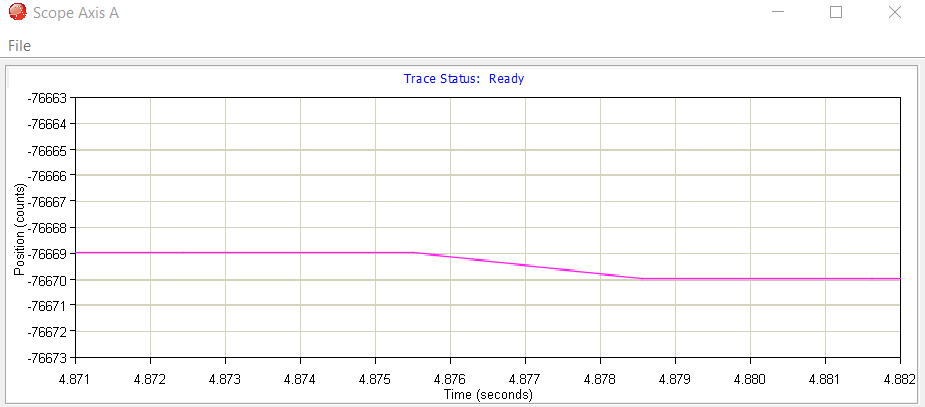
\includegraphics[width=6.46875in]{jira_imgs/3964.png}As seen in the
screenshot, the displacement after the compression load was applied was
about 1 count.

}
\begin{tabular}{p{2cm}p{14cm}}
\toprule
Step 2.8 & Step Execution Status: \textbf{ Pass } \\ \hline
\end{tabular}
 Description \\
{\footnotesize
Confirm that there are no other signs of gross actuator motion.

}
\hdashrule[0.5ex]{\textwidth}{1pt}{3mm}
  Expected Result \\
{\footnotesize
No visual movement, significant motion of the internal linear encoder or
external linear test encoders beyond expected actuator compliance
recorded in the LabView displacement graphs.~

}
\hdashrule[0.5ex]{\textwidth}{1pt}{3mm}
  Actual Result \\
{\footnotesize
Visually, the position of the actuator remained in the center position.

}
\begin{tabular}{p{2cm}p{14cm}}
\toprule
Step 2.9 & Step Execution Status: \textbf{ Pass } \\ \hline
\end{tabular}
 Description \\
{\footnotesize
Reduce the {Compression}⁠ ~force to back to zero load.

}
\hdashrule[0.5ex]{\textwidth}{1pt}{3mm}
  Test Data \\
 {\footnotesize
\textbf{Note:~}In order to reset the load to zero, both the valves
should be set to 0V.

}
\hdashrule[0.5ex]{\textwidth}{1pt}{3mm}
  Expected Result \\
{\footnotesize
{Compression}⁠~ force removed and load cell reading in the lab-view
graph and load cell reader showing zero load.

}
\hdashrule[0.5ex]{\textwidth}{1pt}{3mm}
  Actual Result \\
{\footnotesize
Compression load was removed.

}
\begin{tabular}{p{2cm}p{14cm}}
\toprule
Step 3.0 & Step Execution Status: \textbf{ Pass } \\ \hline
\end{tabular}
 Description \\
{\footnotesize
Record the displacement of the actuator using the external encoder
readings.

}
\hdashrule[0.5ex]{\textwidth}{1pt}{3mm}
  Test Data \\
 {\footnotesize
\textbf{Note:~}The Copley software will display a value based on the
reading from its internal encoder, which may be useful to take note of.
However, the readings reported by the external encoders will validate
the reading of the internal encoder.

}
\hdashrule[0.5ex]{\textwidth}{1pt}{3mm}
  Expected Result \\
{\footnotesize
The final position of the actuator has been determined.\\
If the actuator position has changed significantly (\textgreater{}10
counts or 0.36 deg of motor rotation), the actuator has back-driven.

}
\hdashrule[0.5ex]{\textwidth}{1pt}{3mm}
  Actual Result \\
{\footnotesize
The actuator returns to its ``zero position''\\

\begin{itemize}
\tightlist
\item
  Copley Software: Active Load Position = \textbf{-22.00mm}
\item
  Encoder A (D13B) = 39.29mm
\item
  Encoder B (D0BD) = 39.42mm
\end{itemize}

}
\begin{tabular}{p{2cm}p{14cm}}
\toprule
Step 3.1 & Step Execution Status: \textbf{ Pass } \\ \hline
\end{tabular}
 Description \\
{\footnotesize
Check if all the test results are recorded in excel spreadsheets.

}
\hdashrule[0.5ex]{\textwidth}{1pt}{3mm}
  Test Data \\
 {\footnotesize


}
\hdashrule[0.5ex]{\textwidth}{1pt}{3mm}
  Expected Result \\
{\footnotesize
Test Results are recorded in the excel spreadsheets residing in the
LabView Folder directory.

}
\hdashrule[0.5ex]{\textwidth}{1pt}{3mm}
  Actual Result \\
{\footnotesize
The screenshot of the Copley Control Software can be seen in Step 7. The
data as recorded by the external linear encoders be seen in
the\emph{~Back Drive Test Results - Unmodified Actuator (1).xlsm} excel
file.

}
\begin{tabular}{p{2cm}p{14cm}}
\toprule
Step 3.2 & Step Execution Status: \textbf{ Not Executed } \\ \hline
\end{tabular}
 Description \\
{\footnotesize
Close all the Labview VI files.

}
\hdashrule[0.5ex]{\textwidth}{1pt}{3mm}
  Test Data \\
 {\footnotesize
\textbf{Note:~}Labview can be left open in order to continue to the next
test. However, it may be necessary to reset the application before
starting the next test.

}
\hdashrule[0.5ex]{\textwidth}{1pt}{3mm}
  Expected Result \\
{\footnotesize
All the VI files are closed and Labview 2021 application window closes.

}
\hdashrule[0.5ex]{\textwidth}{1pt}{3mm}
  Actual Result \\
{\footnotesize
The LabView VI was left open to continue the next test.

}

\paragraph{ LVV-T2428 - Hexapod - Actuator Stiffness Test }\mbox{}\\

Version \textbf{1}.
Status \textbf{Approved}.
Open  \href{https://jira.lsstcorp.org/secure/Tests.jspa#/testCase/LVV-T2428}{\textit{ LVV-T2428 } }
test case in Jira.



\textbf{ Preconditions}:\\


Execution status: {\bf Pass }

Final comment:\\The actuator was placed as close to the positive limit switch as
possible when extended and as close to the negative limit switch as
possible when retracted.\\
As a reminder, the reported position of the rotary encoder were
different after the actuator modifications.\\
Negative Limit Switch:

\begin{itemize}
\tightlist
\item
  Copley Software: Active Load Position = \textbf{-36.03mm or
  -36003000counts}
\end{itemize}

Zero Position:

\begin{itemize}
\tightlist
\item
  Copley Software: Active Load Position = \textbf{-22.008mm or -2200875
  counts}
\end{itemize}

Positive Limit Switch:

\begin{itemize}
\tightlist
\item
  Copley Software: Active Load Position = \textbf{-7.515mm or -7515000
  counts}
\end{itemize}

In conclusion, the stiffness of the actuator was seen in the following
positions as follows:

\begin{itemize}
\tightlist
\item
  Zero Position = 101.6N/um
\item
  Negative Limit Switch = 101.4N/um
\item
  Positive Limit Switch = 101.6N/um
\end{itemize}

The results from both the unmodified and modified actuator tests have
been uploaded into docushare. As seen in the Results Summary sheet,
Moog's results showed that the stiffness of the actuator was on average
117N/um. The results from the unmodified actuator stiffness test showed
that the actuator was on average 130N/um. It can be seen that the
actuator is a lot less stiff than MOOG's original results and the
results obtained from the unmodified test. It can be seen in the results
of the attached document that there is not only larger displacement in
the modified actuator test results, but there is a larger delta between
the two encoder positions. An explanation for this may be due to the
fact that the modified design includes a cutout meant for the external
encoder housing that is causing a twisting moment. As a result, this is
causing displacement at a higher rate for one encoder than the other.
This can be seen in the graphs plotting velocity of the encoders vs time
on the Velocity Graphs\emph{~}sheet of the
\href{https://docushare.lsst.org/docushare/dsweb/Services/Document-55068}{\emph{Stiffness
Test Results Modified vs UnModified.xlsx}}file.


Detailed steps results:

\begin{tabular}{p{2cm}p{14cm}}
\toprule
Step 0.4 & Step Execution Status: \textbf{ Pass } \\ \hline
\end{tabular}
 Description \\
{\footnotesize
Note the starting position read by the encoders, while fully {centered}⁠
.

}
\hdashrule[0.5ex]{\textwidth}{1pt}{3mm}
  Test Data \\
 {\footnotesize
\textbf{Note}:\\
Centered = Actuator is at the zero position (Active Load Position =
-40.202mm)\\
Extended~= Actuator is at its positive limit switch (Active Load
Position = -25.904mm)\\
Retracted = Actuator is at its negative limit switch (Active Load
Position = -54.501mm)\\
Modified Actuator-Pressure max= 110

}
\hdashrule[0.5ex]{\textwidth}{1pt}{3mm}
  Expected Result \\
{\footnotesize
Actuator position confirmed by encoder reading in the
LabView.\\[2\baselineskip]

}
\hdashrule[0.5ex]{\textwidth}{1pt}{3mm}
  Actual Result \\
{\footnotesize
Center Position:\\

\begin{itemize}
\tightlist
\item
  Copley Software: Active Load Position = \textbf{-22.008mm or -2200875
  counts}
\item
  Encoder A (D13B) = 39.23mm
\item
  Encoder B (D0BD) = 39.70mm
\end{itemize}

}
\begin{tabular}{p{2cm}p{14cm}}
\toprule
Step 0.4 & Step Execution Status: \textbf{ Pass } \\ \hline
\end{tabular}
 Description \\
{\footnotesize
Note the starting position read by the encoders, while fully {extended}⁠
.

}
\hdashrule[0.5ex]{\textwidth}{1pt}{3mm}
  Test Data \\
 {\footnotesize
\textbf{Note}:\\
Centered = Actuator is at the zero position (Active Load Position =
-40.202mm)\\
Extended~= Actuator is at its positive limit switch (Active Load
Position = -25.904mm)\\
Retracted = Actuator is at its negative limit switch (Active Load
Position = -54.501mm)\\
Modified Actuator-Pressure max= 110

}
\hdashrule[0.5ex]{\textwidth}{1pt}{3mm}
  Expected Result \\
{\footnotesize
Actuator position confirmed by encoder reading in the
LabView.\\[2\baselineskip]

}
\hdashrule[0.5ex]{\textwidth}{1pt}{3mm}
  Actual Result \\
{\footnotesize
Extended Position:\\

\begin{itemize}
\tightlist
\item
  Copley Software: Active Load Position = \textbf{-7.808mm or
  -7808000counts}
\item
  Encoder A (D13B) = 25.11mm
\item
  Encoder B (D0BD) = 25.54mm
\end{itemize}

}
\begin{tabular}{p{2cm}p{14cm}}
\toprule
Step 0.5 & Step Execution Status: \textbf{ Pass } \\ \hline
\end{tabular}
 Description \\
{\footnotesize
Disable Motor Power by pressing the Emergency stop button on the control
box.

}
\hdashrule[0.5ex]{\textwidth}{1pt}{3mm}
  Expected Result \\
{\footnotesize
Motor power disabled.

}
\hdashrule[0.5ex]{\textwidth}{1pt}{3mm}
  Actual Result \\
{\footnotesize
The E-stop of the motor was pressed and the control software was seen to
be disabled on the Copley Control.

}
\begin{tabular}{p{2cm}p{14cm}}
\toprule
Step 0.5 & Step Execution Status: \textbf{ Pass } \\ \hline
\end{tabular}
 Description \\
{\footnotesize
Disable Motor Power by pressing the Emergency stop button on the control
box.

}
\hdashrule[0.5ex]{\textwidth}{1pt}{3mm}
  Expected Result \\
{\footnotesize
Motor power disabled.

}
\hdashrule[0.5ex]{\textwidth}{1pt}{3mm}
  Actual Result \\
{\footnotesize
The E-stop of the motor was pressed and the control software was seen to
be disabled on the Copley Control.

}
\begin{tabular}{p{2cm}p{14cm}}
\toprule
Step 0.6 & Step Execution Status: \textbf{ Pass } \\ \hline
\end{tabular}
 Description \\
{\footnotesize
While fully {centered}⁠: Increase the load on the actuator from 0 kN to
approximately +30kN.

}
\hdashrule[0.5ex]{\textwidth}{1pt}{3mm}
  Test Data \\
 {\footnotesize
\textbf{Note:~}To apply +30kN, set Channel 1 = 4.38V and Channel 0 = 0V.

}
\hdashrule[0.5ex]{\textwidth}{1pt}{3mm}
  Expected Result \\
{\footnotesize
Load cell reader shows the applied +30 kN tension force.\\
LabView displays the voltage being applied.

}
\hdashrule[0.5ex]{\textwidth}{1pt}{3mm}
  Actual Result \\
{\footnotesize
30kN of tension was applied by setting Channel 1 to 8.9V.

}
\begin{tabular}{p{2cm}p{14cm}}
\toprule
Step 0.6 & Step Execution Status: \textbf{ Pass } \\ \hline
\end{tabular}
 Description \\
{\footnotesize
While fully {extended}⁠: Increase the load on the actuator from 0 kN to
approximately +30kN.

}
\hdashrule[0.5ex]{\textwidth}{1pt}{3mm}
  Test Data \\
 {\footnotesize
\textbf{Note:~}To apply +30kN, set Channel 1 = 4.38V and Channel 0 = 0V.

}
\hdashrule[0.5ex]{\textwidth}{1pt}{3mm}
  Expected Result \\
{\footnotesize
Load cell reader shows the applied +30 kN tension force.\\
LabView displays the voltage being applied.

}
\hdashrule[0.5ex]{\textwidth}{1pt}{3mm}
  Actual Result \\
{\footnotesize
30kN of tension was applied by setting Channel 1 to 8.9V.

}
\begin{tabular}{p{2cm}p{14cm}}
\toprule
Step 0.7 & Step Execution Status: \textbf{ Pass } \\ \hline
\end{tabular}
 Description \\
{\footnotesize
While fully {{centered}⁠}: Reduce the load to back to 0kN and then to
-30 kN.

}
\hdashrule[0.5ex]{\textwidth}{1pt}{3mm}
  Test Data \\
 {\footnotesize
\textbf{Note:~}To apply -30kN, set Channel 1 = 4.38V and Channel 0 = 0V.

}
\hdashrule[0.5ex]{\textwidth}{1pt}{3mm}
  Expected Result \\
{\footnotesize
Load cell reader shows the applied 0kN force and the -30kN compression
force.

}
\hdashrule[0.5ex]{\textwidth}{1pt}{3mm}
  Actual Result \\
{\footnotesize
Channel 1 was set back to 0 and then Channel 0 was set to 8.9V to apply
-30kN of force.

}
\begin{tabular}{p{2cm}p{14cm}}
\toprule
Step 0.7 & Step Execution Status: \textbf{ Pass } \\ \hline
\end{tabular}
 Description \\
{\footnotesize
While fully {{extended}⁠}: Reduce the load to back to 0kN and then to
-30 kN.

}
\hdashrule[0.5ex]{\textwidth}{1pt}{3mm}
  Test Data \\
 {\footnotesize
\textbf{Note:~}To apply -30kN, set Channel 1 = 4.38V and Channel 0 = 0V.

}
\hdashrule[0.5ex]{\textwidth}{1pt}{3mm}
  Expected Result \\
{\footnotesize
Load cell reader shows the applied 0kN force and the -30kN compression
force.

}
\hdashrule[0.5ex]{\textwidth}{1pt}{3mm}
  Actual Result \\
{\footnotesize
Channel 1 was set back to 0 and then Channel 0 was set to 8.9V to apply
-30kN of force.

}
\begin{tabular}{p{2cm}p{14cm}}
\toprule
Step 0.8 & Step Execution Status: \textbf{ Pass } \\ \hline
\end{tabular}
 Description \\
{\footnotesize
Record the actual displacement as measured by the two external encoders
as LabView graph (Displacement vs Time).\\[2\baselineskip]

}
\hdashrule[0.5ex]{\textwidth}{1pt}{3mm}
  Expected Result \\
{\footnotesize
Actual displacement measured by the average of the two external encoders
~recorded in the LabView graph.

}
\hdashrule[0.5ex]{\textwidth}{1pt}{3mm}
  Actual Result \\
{\footnotesize
The displacement was recorded into a LabView graph (Displacement vs
Time) for each encoder. By right-clicking on the graphs, we were able to
export the values onto an excel file and plot them against displacement.

}
\begin{tabular}{p{2cm}p{14cm}}
\toprule
Step 0.8 & Step Execution Status: \textbf{ Pass } \\ \hline
\end{tabular}
 Description \\
{\footnotesize
Record the actual displacement as measured by the two external encoders
as LabView graph (Displacement vs Time).\\[2\baselineskip]

}
\hdashrule[0.5ex]{\textwidth}{1pt}{3mm}
  Expected Result \\
{\footnotesize
Actual displacement measured by the average of the two external encoders
~recorded in the LabView graph.

}
\hdashrule[0.5ex]{\textwidth}{1pt}{3mm}
  Actual Result \\
{\footnotesize
The displacement was recorded into a LabView graph (Displacement vs
Time) for each encoder. By right-clicking on the graphs, we were able to
export the values onto an excel file and plot them against displacement.

}
\begin{tabular}{p{2cm}p{14cm}}
\toprule
Step 0.9 & Step Execution Status: \textbf{ Pass } \\ \hline
\end{tabular}
 Description \\
{\footnotesize
View the force vs displacement plot in the Labview.

}
\hdashrule[0.5ex]{\textwidth}{1pt}{3mm}
  Expected Result \\
{\footnotesize
The expected actuator stiffness is \textgreater{}= 134 N/um at center
stroke.~\\[2\baselineskip]

}
\hdashrule[0.5ex]{\textwidth}{1pt}{3mm}
  Actual Result \\
{\footnotesize
The following plot was created in Excel using the exported values from
LabView:\\
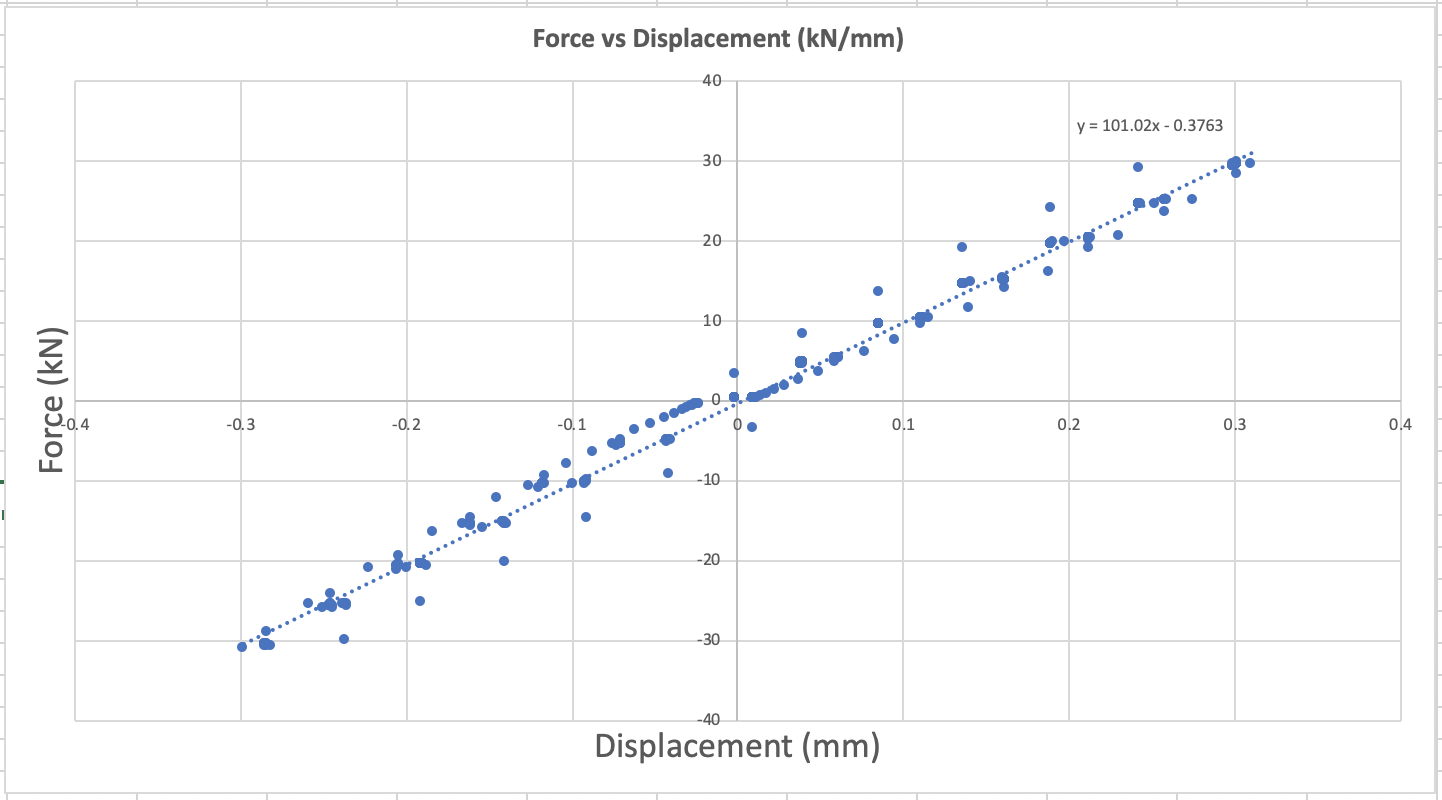
\includegraphics[width=5.98958in]{jira_imgs/4092.png}\\
This is one iteration of the stiffness results taken in the zero
position. This test was repeated three times in total initially in the
zero position to ensure that the results were consistent. As a result,
the average stiffness of the actuator while in the zero position was
calculated to be 101.6kN/mm.

}
\begin{tabular}{p{2cm}p{14cm}}
\toprule
Step 0.9 & Step Execution Status: \textbf{ Pass } \\ \hline
\end{tabular}
 Description \\
{\footnotesize
View the force vs displacement plot in the Labview.

}
\hdashrule[0.5ex]{\textwidth}{1pt}{3mm}
  Expected Result \\
{\footnotesize
The expected actuator stiffness is \textgreater{}= 134 N/um at center
stroke.~\\[2\baselineskip]

}
\hdashrule[0.5ex]{\textwidth}{1pt}{3mm}
  Actual Result \\
{\footnotesize
The following plot was created in Excel using the exported values from
LabView:\\
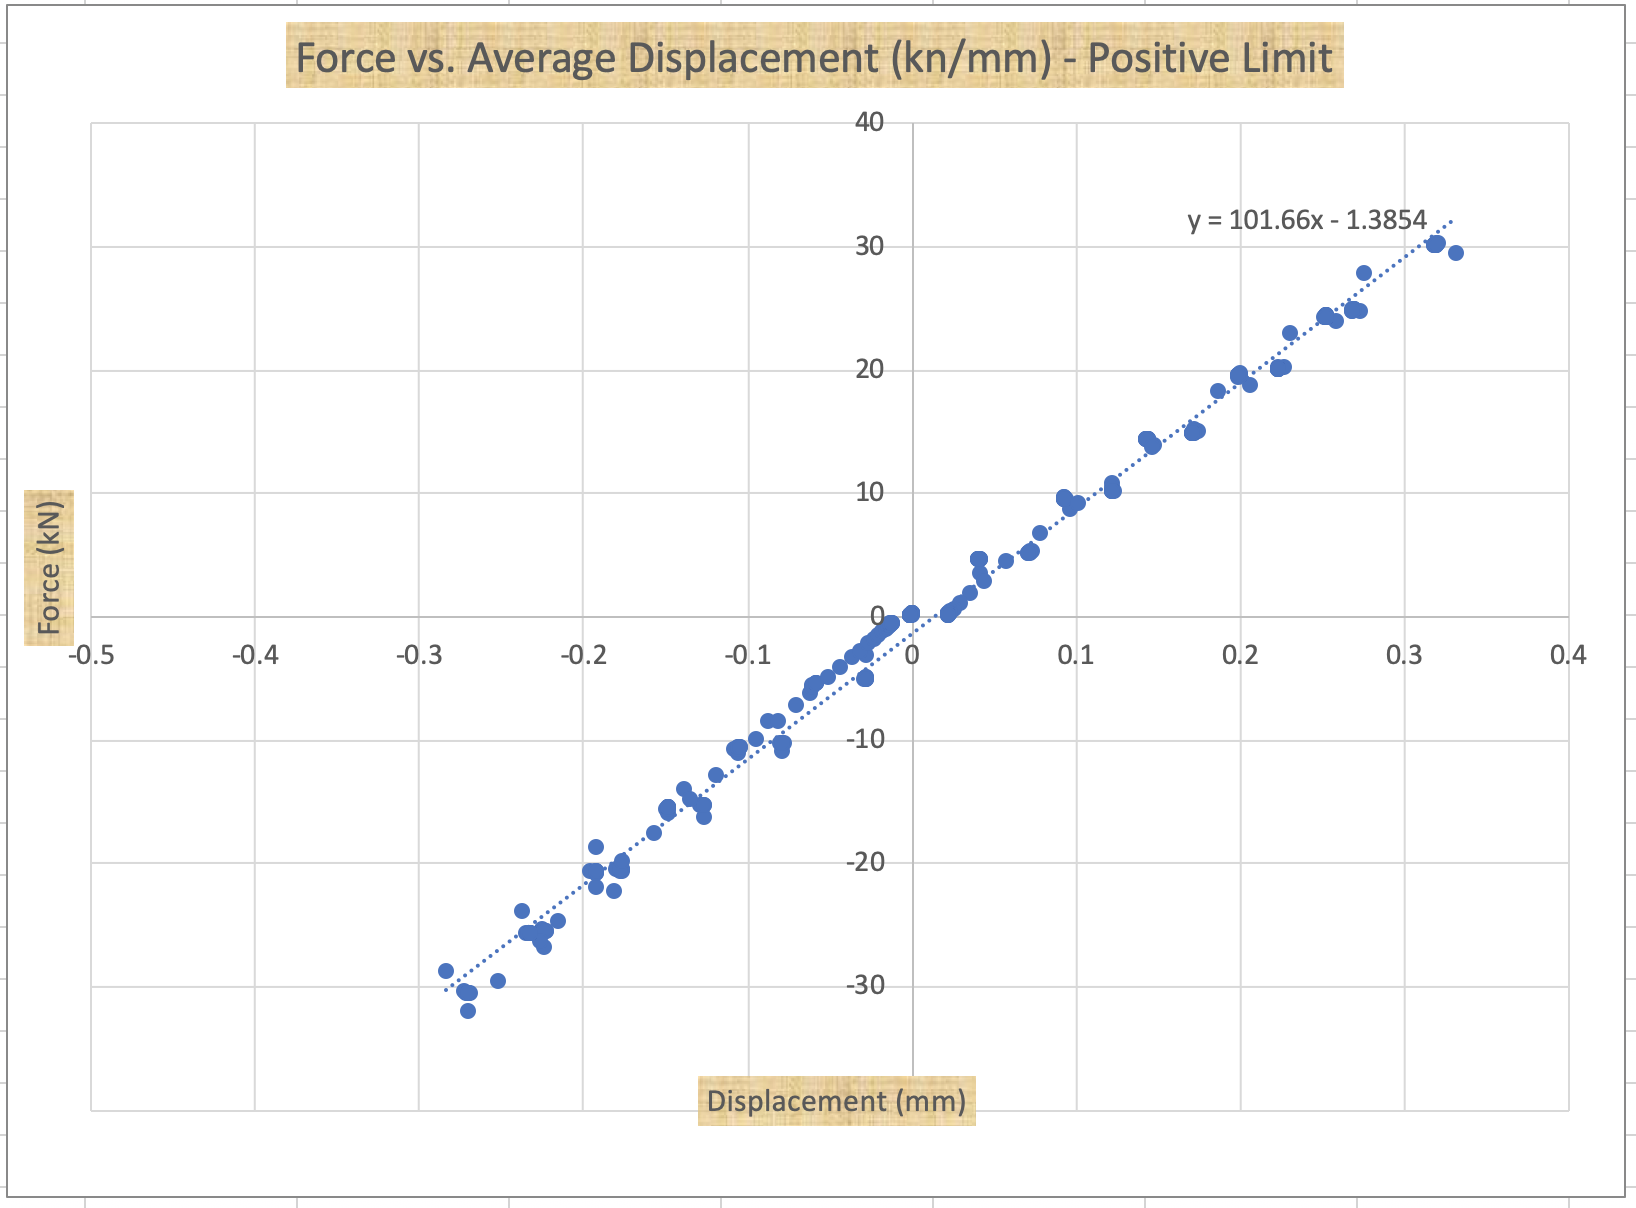
\includegraphics[width=5.98958in]{jira_imgs/4101.png}From this plot, the
overall stiffness can be seen to be 101.66kN/mm.

}
\begin{tabular}{p{2cm}p{14cm}}
\toprule
Step 1.1 & Step Execution Status: \textbf{ Pass } \\ \hline
\end{tabular}
 Description \\
{\footnotesize
Open Labview 2021 in the computer used for Test Setup.

}
\hdashrule[0.5ex]{\textwidth}{1pt}{3mm}
  Test Data \\
 {\footnotesize
\textbf{Note:~}The first three steps are conditional because these steps
are included as part of the Test Setup procedure and may not be
necessary if LabView is still open.

}
\hdashrule[0.5ex]{\textwidth}{1pt}{3mm}
  Expected Result \\
{\footnotesize
Labview 2021 opens successfully.

}
\hdashrule[0.5ex]{\textwidth}{1pt}{3mm}
  Actual Result \\
{\footnotesize
Labview was opened successfully.

}
\begin{tabular}{p{2cm}p{14cm}}
\toprule
Step 1.2 & Step Execution Status: \textbf{ Pass } \\ \hline
\end{tabular}
 Description \\
{\footnotesize
Run the following VI's:

\begin{itemize}
\tightlist
\item
  Encoder A (D13B) and Load Cell.vi
\item
  Encoder B (D0BD).vi
\end{itemize}

}
\hdashrule[0.5ex]{\textwidth}{1pt}{3mm}
  Expected Result \\
{\footnotesize
Front panel of VI's open without any error.

}
\hdashrule[0.5ex]{\textwidth}{1pt}{3mm}
  Actual Result \\
{\footnotesize
VI's are open.

}
\begin{tabular}{p{2cm}p{14cm}}
\toprule
Step 1.3 & Step Execution Status: \textbf{ Pass } \\ \hline
\end{tabular}
 Description \\
{\footnotesize
Click Run button on the block diagram toolbar of the Labview VI front
panel.

}
\hdashrule[0.5ex]{\textwidth}{1pt}{3mm}
  Expected Result \\
{\footnotesize
LabView VI and associated sub Vi runs successfully. The graphs should
start to be populated with data once the run button is pressed.~

}
\hdashrule[0.5ex]{\textwidth}{1pt}{3mm}
  Actual Result \\
{\footnotesize
The Vi's are operational with no error.

}
\begin{tabular}{p{2cm}p{14cm}}
\toprule
Step 2.0 & Step Execution Status: \textbf{ Pass } \\ \hline
\end{tabular}
 Description \\
{\footnotesize
Check if all the test results are recorded in excel spreadsheets.

}
\hdashrule[0.5ex]{\textwidth}{1pt}{3mm}
  Expected Result \\
{\footnotesize
Test Results are recorded in the excel spreadsheets residing in the
LabView Folder directory.

}
\hdashrule[0.5ex]{\textwidth}{1pt}{3mm}
  Actual Result \\
{\footnotesize
The data was exported into the \emph{Stiffness Test Results Modified vs
UnModified.xlsx~}file and uploaded to docushare.

}
\begin{tabular}{p{2cm}p{14cm}}
\toprule
Step 2.1 & Step Execution Status: \textbf{ Not Executed } \\ \hline
\end{tabular}
 Description \\
{\footnotesize
Close all the Labview VI files.

}
\hdashrule[0.5ex]{\textwidth}{1pt}{3mm}
  Test Data \\
 {\footnotesize
\textbf{Note:~}Labview can be left open in order to continue to the next
test. However, it may be necessary to reset the application before
starting the next test.

}
\hdashrule[0.5ex]{\textwidth}{1pt}{3mm}
  Expected Result \\
{\footnotesize
All the VI files are closed and Labview 2021 application window closes.

}
\hdashrule[0.5ex]{\textwidth}{1pt}{3mm}
  Actual Result \\
{\footnotesize
Labview was left open in order to continue test.

}
\begin{tabular}{p{2cm}p{14cm}}
\toprule
Step 2.1 & Step Execution Status: \textbf{ Pass } \\ \hline
\end{tabular}
 Description \\
{\footnotesize
Open Labview 2021 in the computer used for Test Setup.

}
\hdashrule[0.5ex]{\textwidth}{1pt}{3mm}
  Test Data \\
 {\footnotesize
\textbf{Note:~}The first three steps are conditional because these steps
are included as part of the Test Setup procedure and may not be
necessary if LabView is still open.

}
\hdashrule[0.5ex]{\textwidth}{1pt}{3mm}
  Expected Result \\
{\footnotesize
Labview 2021 opens successfully.

}
\hdashrule[0.5ex]{\textwidth}{1pt}{3mm}
  Actual Result \\
{\footnotesize
Labview was already open

}
\begin{tabular}{p{2cm}p{14cm}}
\toprule
Step 2.2 & Step Execution Status: \textbf{ Pass } \\ \hline
\end{tabular}
 Description \\
{\footnotesize
Run the following VI's:

\begin{itemize}
\tightlist
\item
  Encoder A (D13B) and Load Cell.vi
\item
  Encoder B (D0BD).vi
\end{itemize}

}
\hdashrule[0.5ex]{\textwidth}{1pt}{3mm}
  Expected Result \\
{\footnotesize
Front panel of VI's open without any error.

}
\hdashrule[0.5ex]{\textwidth}{1pt}{3mm}
  Actual Result \\
{\footnotesize
VI's are open.

}
\begin{tabular}{p{2cm}p{14cm}}
\toprule
Step 2.3 & Step Execution Status: \textbf{ Pass } \\ \hline
\end{tabular}
 Description \\
{\footnotesize
Click Run button on the block diagram toolbar of the Labview VI front
panel.

}
\hdashrule[0.5ex]{\textwidth}{1pt}{3mm}
  Expected Result \\
{\footnotesize
LabView VI and associated sub Vi runs successfully. The graphs should
start to be populated with data once the run button is pressed.~

}
\hdashrule[0.5ex]{\textwidth}{1pt}{3mm}
  Actual Result \\
{\footnotesize
The Vi's are operational with no error.

}
\begin{tabular}{p{2cm}p{14cm}}
\toprule
Step 3.0 & Step Execution Status: \textbf{ Pass } \\ \hline
\end{tabular}
 Description \\
{\footnotesize
Check if all the test results are recorded in excel spreadsheets.

}
\hdashrule[0.5ex]{\textwidth}{1pt}{3mm}
  Expected Result \\
{\footnotesize
Test Results are recorded in the excel spreadsheets residing in the
LabView Folder directory.

}
\hdashrule[0.5ex]{\textwidth}{1pt}{3mm}
  Actual Result \\
{\footnotesize
The data was exported into the \emph{Stiffness Test Results Modified vs
UnModified.xlsx~}file and uploaded to docushare.

}
\begin{tabular}{p{2cm}p{14cm}}
\toprule
Step 3.1 & Step Execution Status: \textbf{ Not Executed } \\ \hline
\end{tabular}
 Description \\
{\footnotesize
Close all the Labview VI files.

}
\hdashrule[0.5ex]{\textwidth}{1pt}{3mm}
  Test Data \\
 {\footnotesize
\textbf{Note:~}Labview can be left open in order to continue to the next
test. However, it may be necessary to reset the application before
starting the next test.

}
\hdashrule[0.5ex]{\textwidth}{1pt}{3mm}
  Expected Result \\
{\footnotesize
All the VI files are closed and Labview 2021 application window closes.

}
\hdashrule[0.5ex]{\textwidth}{1pt}{3mm}
  Actual Result \\
{\footnotesize
Labview was left open in order to continue test.

}
\begin{tabular}{p{2cm}p{14cm}}
\toprule
Step 3.1 & Step Execution Status: \textbf{ Pass } \\ \hline
\end{tabular}
 Description \\
{\footnotesize
Open Labview 2021 in the computer used for Test Setup.

}
\hdashrule[0.5ex]{\textwidth}{1pt}{3mm}
  Test Data \\
 {\footnotesize
\textbf{Note:~}The first three steps are conditional because these steps
are included as part of the Test Setup procedure and may not be
necessary if LabView is still open.

}
\hdashrule[0.5ex]{\textwidth}{1pt}{3mm}
  Expected Result \\
{\footnotesize
Labview 2021 opens successfully.

}
\hdashrule[0.5ex]{\textwidth}{1pt}{3mm}
  Actual Result \\
{\footnotesize
Labview was already open

}
\begin{tabular}{p{2cm}p{14cm}}
\toprule
Step 3.2 & Step Execution Status: \textbf{ Pass } \\ \hline
\end{tabular}
 Description \\
{\footnotesize
Run the following VI's:

\begin{itemize}
\tightlist
\item
  Encoder A (D13B) and Load Cell.vi
\item
  Encoder B (D0BD).vi
\end{itemize}

}
\hdashrule[0.5ex]{\textwidth}{1pt}{3mm}
  Expected Result \\
{\footnotesize
Front panel of VI's open without any error.

}
\hdashrule[0.5ex]{\textwidth}{1pt}{3mm}
  Actual Result \\
{\footnotesize
VI's are open.

}
\begin{tabular}{p{2cm}p{14cm}}
\toprule
Step 3.3 & Step Execution Status: \textbf{ Pass } \\ \hline
\end{tabular}
 Description \\
{\footnotesize
Click Run button on the block diagram toolbar of the Labview VI front
panel.

}
\hdashrule[0.5ex]{\textwidth}{1pt}{3mm}
  Expected Result \\
{\footnotesize
LabView VI and associated sub Vi runs successfully. The graphs should
start to be populated with data once the run button is pressed.~

}
\hdashrule[0.5ex]{\textwidth}{1pt}{3mm}
  Actual Result \\
{\footnotesize
The Vi's are operational with no error.

}
\begin{tabular}{p{2cm}p{14cm}}
\toprule
Step 3.4 & Step Execution Status: \textbf{ Pass } \\ \hline
\end{tabular}
 Description \\
{\footnotesize
Note the starting position read by the encoders, while fully
{retracted}⁠ .

}
\hdashrule[0.5ex]{\textwidth}{1pt}{3mm}
  Test Data \\
 {\footnotesize
\textbf{Note}:\\
Centered = Actuator is at the zero position (Active Load Position =
-40.202mm)\\
Extended~= Actuator is at its positive limit switch (Active Load
Position = -25.904mm)\\
Retracted = Actuator is at its negative limit switch (Active Load
Position = -54.501mm)\\
Modified Actuator-Pressure max= 110

}
\hdashrule[0.5ex]{\textwidth}{1pt}{3mm}
  Expected Result \\
{\footnotesize
Actuator position confirmed by encoder reading in the
LabView.\\[2\baselineskip]

}
\hdashrule[0.5ex]{\textwidth}{1pt}{3mm}
  Actual Result \\
{\footnotesize
Extended Position:\\

\begin{itemize}
\tightlist
\item
  Encoder A (D13B) = 53.29mm
\item
  Encoder B (D0BD) = 43.74mm
\end{itemize}

}
\begin{tabular}{p{2cm}p{14cm}}
\toprule
Step 3.5 & Step Execution Status: \textbf{ Pass } \\ \hline
\end{tabular}
 Description \\
{\footnotesize
Disable Motor Power by pressing the Emergency stop button on the control
box.

}
\hdashrule[0.5ex]{\textwidth}{1pt}{3mm}
  Expected Result \\
{\footnotesize
Motor power disabled.

}
\hdashrule[0.5ex]{\textwidth}{1pt}{3mm}
  Actual Result \\
{\footnotesize
The E-stop of the motor was pressed and the control software was seen to
be disabled on the Copley Control.

}
\begin{tabular}{p{2cm}p{14cm}}
\toprule
Step 3.6 & Step Execution Status: \textbf{ Pass } \\ \hline
\end{tabular}
 Description \\
{\footnotesize
While fully {retracted}⁠: Increase the load on the actuator from 0 kN to
approximately +30kN.

}
\hdashrule[0.5ex]{\textwidth}{1pt}{3mm}
  Test Data \\
 {\footnotesize
\textbf{Note:~}To apply +30kN, set Channel 1 = 4.38V and Channel 0 = 0V.

}
\hdashrule[0.5ex]{\textwidth}{1pt}{3mm}
  Expected Result \\
{\footnotesize
Load cell reader shows the applied +30 kN tension force.\\
LabView displays the voltage being applied.

}
\hdashrule[0.5ex]{\textwidth}{1pt}{3mm}
  Actual Result \\
{\footnotesize
30kN of tension was applied by setting Channel 1 to 8.9V.

}
\begin{tabular}{p{2cm}p{14cm}}
\toprule
Step 3.7 & Step Execution Status: \textbf{ Pass } \\ \hline
\end{tabular}
 Description \\
{\footnotesize
While fully {{retracted}⁠}: Reduce the load to back to 0kN and then to
-30 kN.

}
\hdashrule[0.5ex]{\textwidth}{1pt}{3mm}
  Test Data \\
 {\footnotesize
\textbf{Note:~}To apply -30kN, set Channel 1 = 4.38V and Channel 0 = 0V.

}
\hdashrule[0.5ex]{\textwidth}{1pt}{3mm}
  Expected Result \\
{\footnotesize
Load cell reader shows the applied 0kN force and the -30kN compression
force.

}
\hdashrule[0.5ex]{\textwidth}{1pt}{3mm}
  Actual Result \\
{\footnotesize
Retraced Position:\\

\begin{itemize}
\tightlist
\item
  Copley Software: Active Load Position = \textbf{-36.03mm or
  -36003000counts}
\item
  Encoder A (D13B) = 53.28mm
\item
  Encoder B (D0BD) = 53.73mm
\end{itemize}

}
\begin{tabular}{p{2cm}p{14cm}}
\toprule
Step 3.8 & Step Execution Status: \textbf{ Pass } \\ \hline
\end{tabular}
 Description \\
{\footnotesize
Record the actual displacement as measured by the two external encoders
as LabView graph (Displacement vs Time).\\[2\baselineskip]

}
\hdashrule[0.5ex]{\textwidth}{1pt}{3mm}
  Expected Result \\
{\footnotesize
Actual displacement measured by the average of the two external encoders
~recorded in the LabView graph.

}
\hdashrule[0.5ex]{\textwidth}{1pt}{3mm}
  Actual Result \\
{\footnotesize
The displacement was recorded into a LabView graph (Displacement vs
Time) for each encoder. By right-clicking on the graphs, we were able to
export the values onto an excel file and plot them against displacement.

}
\begin{tabular}{p{2cm}p{14cm}}
\toprule
Step 3.9 & Step Execution Status: \textbf{ Pass } \\ \hline
\end{tabular}
 Description \\
{\footnotesize
View the force vs displacement plot in the Labview.

}
\hdashrule[0.5ex]{\textwidth}{1pt}{3mm}
  Expected Result \\
{\footnotesize
The expected actuator stiffness is \textgreater{}= 134 N/um at center
stroke.~\\[2\baselineskip]

}
\hdashrule[0.5ex]{\textwidth}{1pt}{3mm}
  Actual Result \\
{\footnotesize
The following plot was created in Excel using the exported values from
LabView:\\
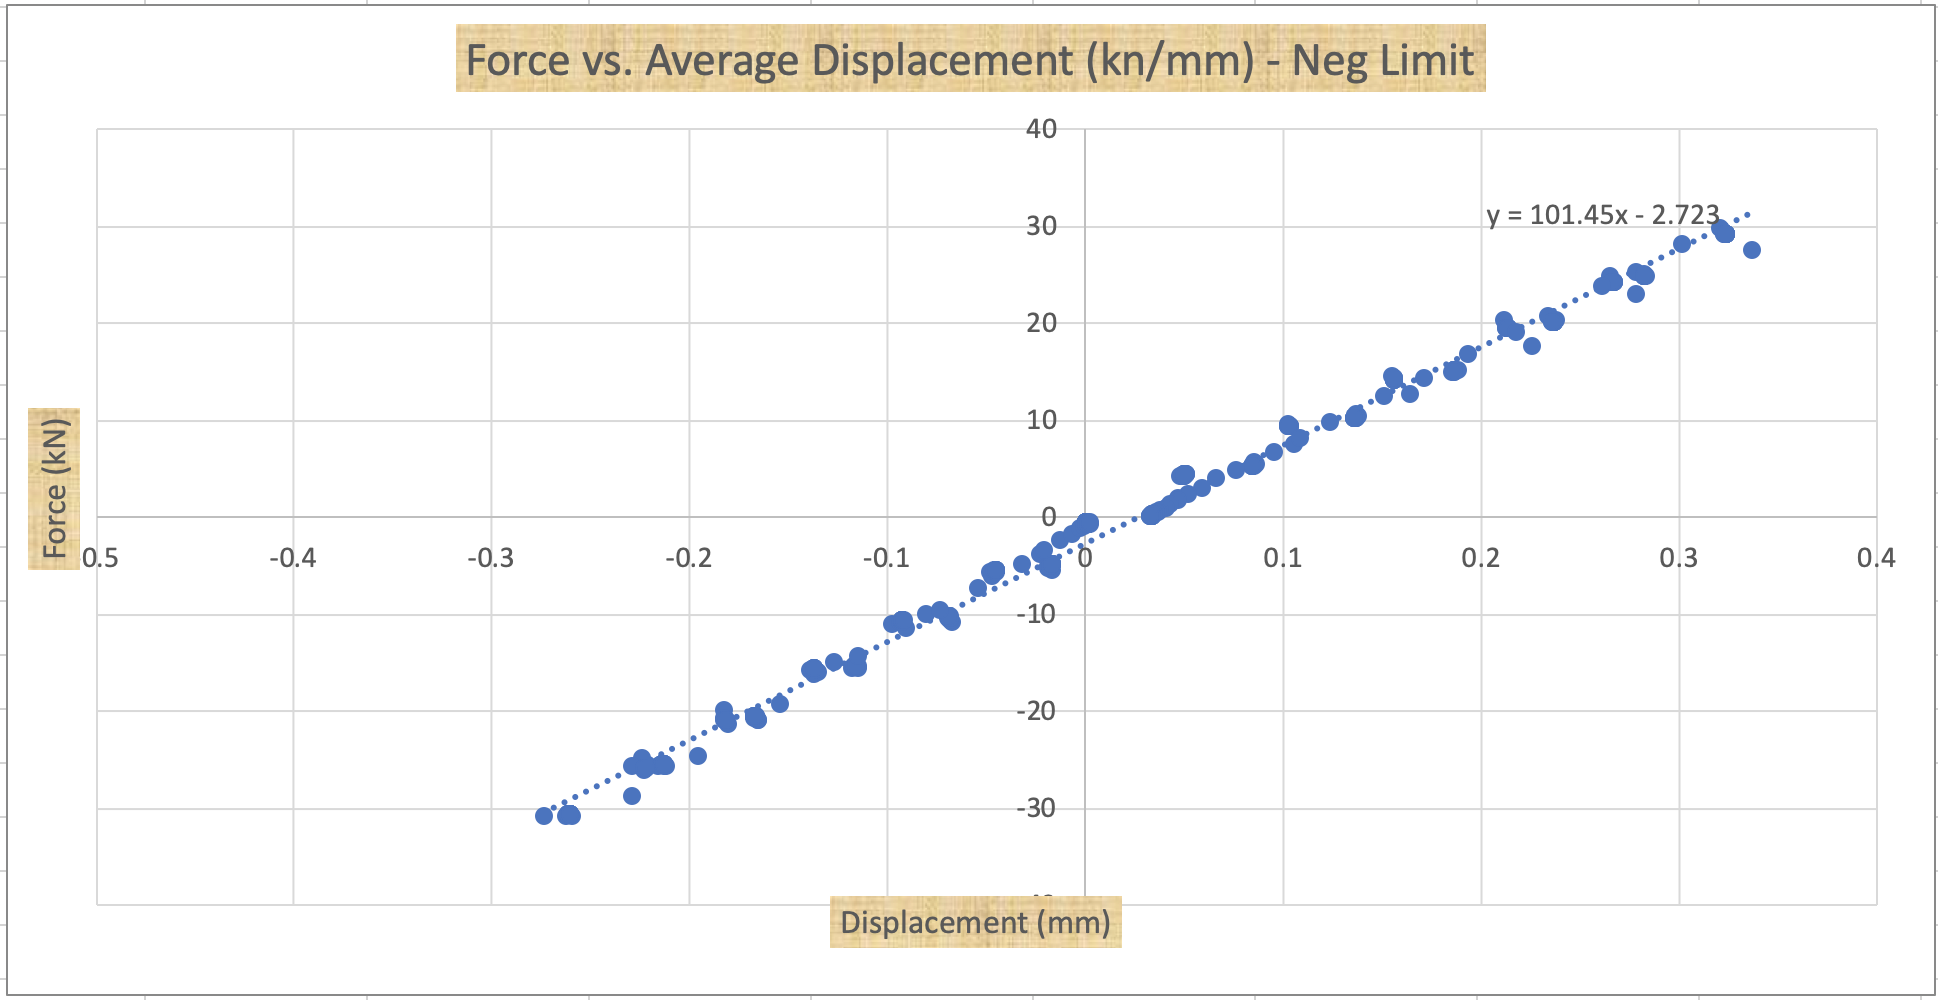
\includegraphics[width=5.98958in]{jira_imgs/4100.png}\\
From this plot, the overall stiffness can be seen to be 101.45kN/mm.

}
\begin{tabular}{p{2cm}p{14cm}}
\toprule
Step 4.0 & Step Execution Status: \textbf{ Pass } \\ \hline
\end{tabular}
 Description \\
{\footnotesize
Check if all the test results are recorded in excel spreadsheets.

}
\hdashrule[0.5ex]{\textwidth}{1pt}{3mm}
  Expected Result \\
{\footnotesize
Test Results are recorded in the excel spreadsheets residing in the
LabView Folder directory.

}
\hdashrule[0.5ex]{\textwidth}{1pt}{3mm}
  Actual Result \\
{\footnotesize
The data was exported into the \emph{Stiffness Test Results Modified vs
UnModified.xlsx~}file and uploaded to docushare.

}
\begin{tabular}{p{2cm}p{14cm}}
\toprule
Step 4.1 & Step Execution Status: \textbf{ Not Executed } \\ \hline
\end{tabular}
 Description \\
{\footnotesize
Close all the Labview VI files.

}
\hdashrule[0.5ex]{\textwidth}{1pt}{3mm}
  Test Data \\
 {\footnotesize
\textbf{Note:~}Labview can be left open in order to continue to the next
test. However, it may be necessary to reset the application before
starting the next test.

}
\hdashrule[0.5ex]{\textwidth}{1pt}{3mm}
  Expected Result \\
{\footnotesize
All the VI files are closed and Labview 2021 application window closes.

}
\hdashrule[0.5ex]{\textwidth}{1pt}{3mm}
  Actual Result \\
{\footnotesize
Labview was left open in order to continue test.

}

\paragraph{ LVV-T2437 - Hexapod - Actuator Movement Test }\mbox{}\\

Version \textbf{1}.
Status \textbf{Approved}.
Open  \href{https://jira.lsstcorp.org/secure/Tests.jspa#/testCase/LVV-T2437}{\textit{ LVV-T2437 } }
test case in Jira.

The purpose of this test will be to verify that the actuators are able
to move within their velocity and acceleration limits. Furthermore,
during the moves, we will also be verifying that the actuators do not
take more than 2 seconds to settle into place.~

\textbf{ Preconditions}:\\


Execution status: {\bf Pass }

Final comment:\\Similar to MOOG's original procedure and the unmodified actuator
movement test, the settling time started when the actuator had reached
its commanded position of +/-5mm and ended when the displacement was
within 0.001mm of that position. As seen in the results of this test
case, the actuator was capable of accurately reaching the +/-5mm
commanded position and the settling time was again seen to be less than
2 seconds. This can be seen in the attached
\href{https://docushare.lsst.org/docushare/dsweb/Services/Document-55079}{\emph{Movement
Test Results - Modified Actuator.xlsx}}\emph{~}excel file.\\
The results of both tension and compression were combined in order to
observe the actuator movement throughout the full test.


Detailed steps results:

\begin{tabular}{p{2cm}p{14cm}}
\toprule
Step 1 & Step Execution Status: \textbf{ Pass } \\ \hline
\end{tabular}
 Description \\
{\footnotesize
Open Labview 2021 in the computer used for Test Setup.

}
\hdashrule[0.5ex]{\textwidth}{1pt}{3mm}
  Test Data \\
 {\footnotesize
The first three steps are conditional because these steps are included
as part of the Test Setup procedure and may not be necessary if LabView
is still open.

}
\hdashrule[0.5ex]{\textwidth}{1pt}{3mm}
  Expected Result \\
{\footnotesize
Labview 2021 opens successfully.

}
\hdashrule[0.5ex]{\textwidth}{1pt}{3mm}
  Actual Result \\
{\footnotesize
Labview was opened successfully.

}
\begin{tabular}{p{2cm}p{14cm}}
\toprule
Step 2 & Step Execution Status: \textbf{ Pass } \\ \hline
\end{tabular}
 Description \\
{\footnotesize
Run the following VI's:

\begin{itemize}
\tightlist
\item
  Encoder A (D13B) and Load Cell.vi
\item
  Encoder B (D0BD).vi
\end{itemize}

}
\hdashrule[0.5ex]{\textwidth}{1pt}{3mm}
  Expected Result \\
{\footnotesize
Front panel of VI's open without any error.

}
\hdashrule[0.5ex]{\textwidth}{1pt}{3mm}
  Actual Result \\
{\footnotesize
LabView and the required VI's were already opened at the start of the
execution of this test cycle.

}
\begin{tabular}{p{2cm}p{14cm}}
\toprule
Step 3 & Step Execution Status: \textbf{ Pass } \\ \hline
\end{tabular}
 Description \\
{\footnotesize
Click Run button on the on the block diagram toolbar of the Labview VI
front panel.

}
\hdashrule[0.5ex]{\textwidth}{1pt}{3mm}
  Expected Result \\
{\footnotesize
LabView VI and associated sub Vi runs successfully. The graphs should
start to be populated with data once the run button is pressed.

}
\hdashrule[0.5ex]{\textwidth}{1pt}{3mm}
  Actual Result \\
{\footnotesize
LabView was ran without any issue.

}
\begin{tabular}{p{2cm}p{14cm}}
\toprule
Step 4 & Step Execution Status: \textbf{ Pass } \\ \hline
\end{tabular}
 Description \\
{\footnotesize
Apply a -15kN compression load by using the LabView function to increase
the air supply value of 2.19V to the compression valve.

}
\hdashrule[0.5ex]{\textwidth}{1pt}{3mm}
  Test Data \\
 {\footnotesize


}
\hdashrule[0.5ex]{\textwidth}{1pt}{3mm}
  Expected Result \\
{\footnotesize
The LabView load graph (Load vs Time) shows -15 KN compression load
applied.

}
\hdashrule[0.5ex]{\textwidth}{1pt}{3mm}
  Actual Result \\
{\footnotesize
The actuator was in the following position at the start of the test:\\

\begin{itemize}
\tightlist
\item
  Encoder A (D13B) = 45.29mm
\item
  Encoder B (D0BD) = 45.72mm
\end{itemize}

A -15kN compression load was applied by setting Channel 0 = 4.38

}
\begin{tabular}{p{2cm}p{14cm}}
\toprule
Step 5 & Step Execution Status: \textbf{ Pass } \\ \hline
\end{tabular}
 Description \\
{\footnotesize
Within the copley software, set the maximum actuator velocity to +/-0.5
mm/s.

}
\hdashrule[0.5ex]{\textwidth}{1pt}{3mm}
  Expected Result \\
{\footnotesize
The maximum velocity is set to 0.5mm/s.

}
\hdashrule[0.5ex]{\textwidth}{1pt}{3mm}
  Actual Result \\
{\footnotesize
The velocity limit could not be changed but was already set to 0.5mm/s

}
\begin{tabular}{p{2cm}p{14cm}}
\toprule
Step 6 & Step Execution Status: \textbf{ Pass } \\ \hline
\end{tabular}
 Description \\
{\footnotesize
Within the copley software, set the actuator acceleration and
deceleration limits to 0.5mm/s\^{}2.

}
\hdashrule[0.5ex]{\textwidth}{1pt}{3mm}
  Expected Result \\
{\footnotesize
The maximum acceleration is set to 0.5mm/s\^{}2.

}
\hdashrule[0.5ex]{\textwidth}{1pt}{3mm}
  Actual Result \\
{\footnotesize
The acceleration and deceleration limits could not be changed but were
already set to 0.5mm/s\^{}s

}
\begin{tabular}{p{2cm}p{14cm}}
\toprule
Step 7 & Step Execution Status: \textbf{ Pass } \\ \hline
\end{tabular}
 Description \\
{\footnotesize
Using the copley software, command the actuator to move relatively +5mm.

}
\hdashrule[0.5ex]{\textwidth}{1pt}{3mm}
  Expected Result \\
{\footnotesize
The Labview graph (Position vs Time) shows the actuator travels 0.342mm
in 2 seconds or less.

}
\hdashrule[0.5ex]{\textwidth}{1pt}{3mm}
  Actual Result \\
{\footnotesize
The actuator reached the following position:\\

\begin{itemize}
\tightlist
\item
  Encoder A (D13B) = 40.19mm
\item
  Encoder B (D0BD) = 40.68mm
\end{itemize}

}
\begin{tabular}{p{2cm}p{14cm}}
\toprule
Step 8 & Step Execution Status: \textbf{ Pass } \\ \hline
\end{tabular}
 Description \\
{\footnotesize
Verify the actuator does not move after reaching the commanded position
by checking the Labview graph (Position vs. Time).

}
\hdashrule[0.5ex]{\textwidth}{1pt}{3mm}
  Expected Result \\
{\footnotesize
The labview graph(Position vs Time) shows the actuator is no longer in
motion.

}
\hdashrule[0.5ex]{\textwidth}{1pt}{3mm}
  Actual Result \\
{\footnotesize
It can roughly be seen from the first half of the following plot that
once that there was no movement after the actuator had reached its
commanded position.~~\\
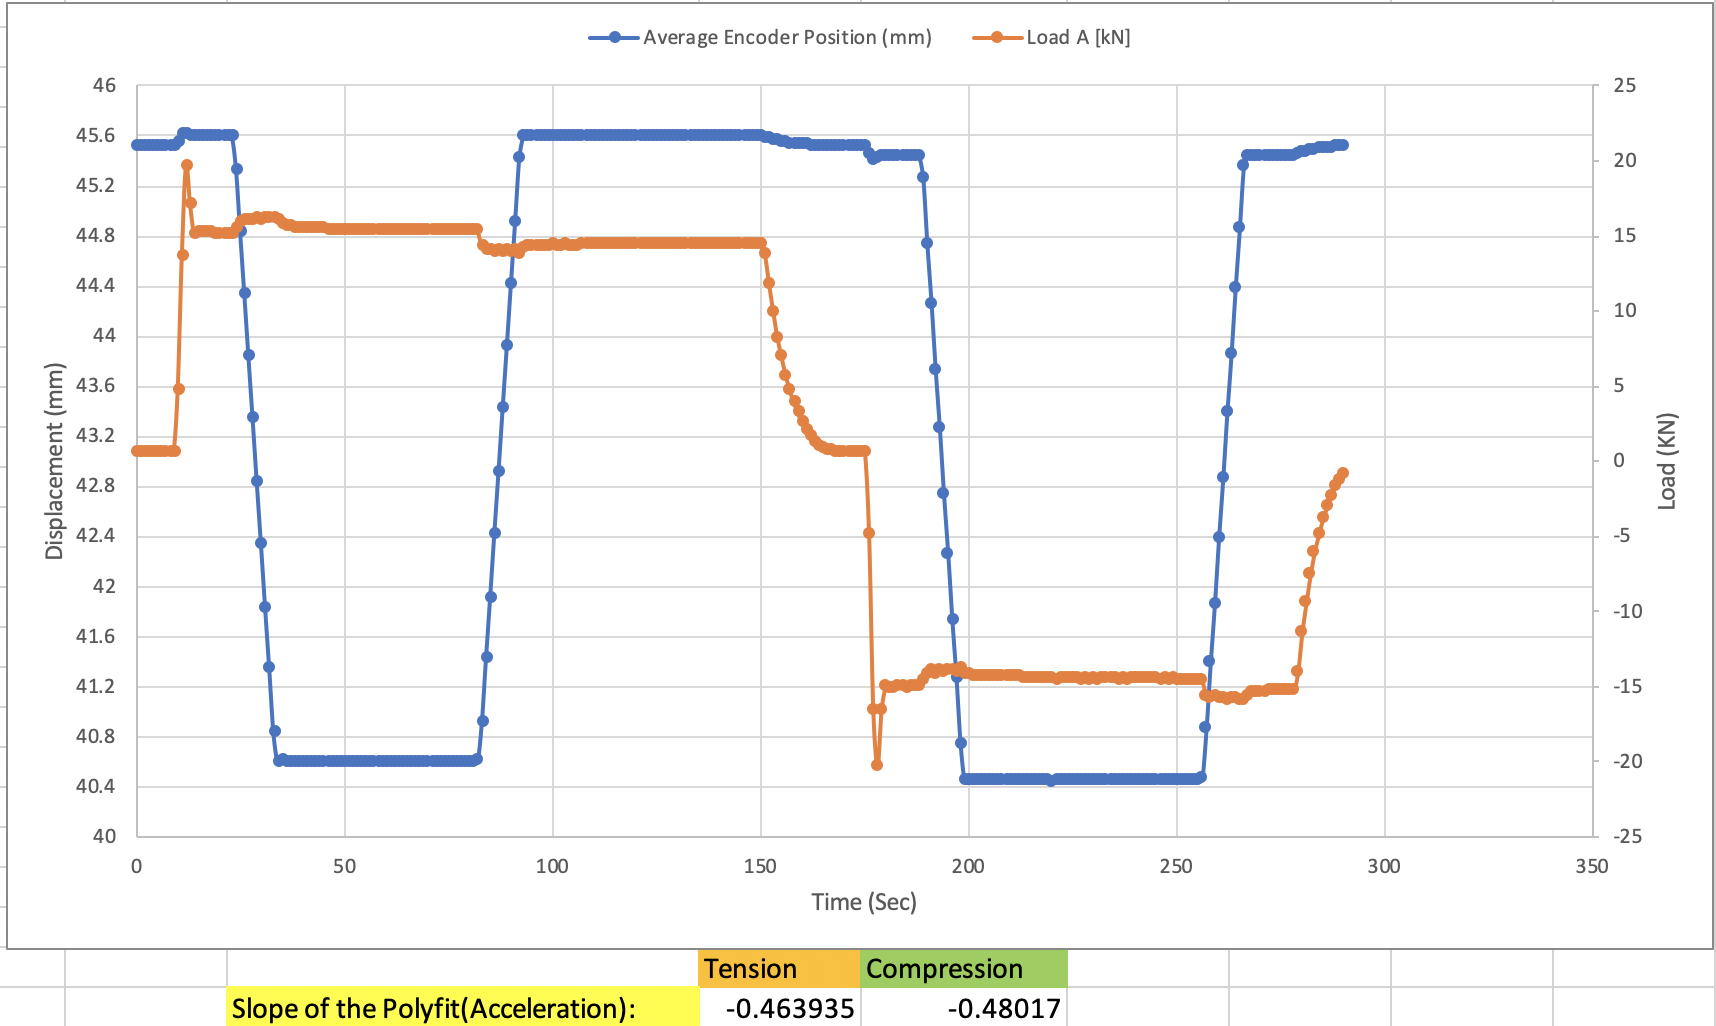
\includegraphics[width=5.98958in]{jira_imgs/4102.png}After Encoder A
reached 40.193mm and Encoder B reached 40.689mm, it took about 2 seconds
for the actuator to settle to within 0.001mm. In 2 seconds, Encoder A
was seen to initially reach 40.193mm, move to 40.188mm and remain
settled at 40.188mm. In 2 seconds, Encoder B was seen to initially reach
40.689mm, move to 40.685mm and remain settled at 40.685mm.

}
\begin{tabular}{p{2cm}p{14cm}}
\toprule
Step 9 & Step Execution Status: \textbf{ Pass } \\ \hline
\end{tabular}
 Description \\
{\footnotesize
Using the copley software, command the actuator to move -5mm
(relatively), returning the original position.

}
\hdashrule[0.5ex]{\textwidth}{1pt}{3mm}
  Test Data \\
 {\footnotesize
\textbf{Note:~}Since the velocity or acceleration limits have not
changed, this should take the same amount of time.

}
\hdashrule[0.5ex]{\textwidth}{1pt}{3mm}
  Expected Result \\
{\footnotesize
The labview graph (Position vs Time) shows the actuator moves back 5mm
in less than 2 seconds.

}
\hdashrule[0.5ex]{\textwidth}{1pt}{3mm}
  Actual Result \\
{\footnotesize
The actuator was returned to the following position:\\

\begin{itemize}
\tightlist
\item
  Encoder A (D13B) = 45.27mm
\item
  Encoder B (D0BD) = 45.74mm
\end{itemize}

}
\begin{tabular}{p{2cm}p{14cm}}
\toprule
Step 10 & Step Execution Status: \textbf{ Pass } \\ \hline
\end{tabular}
 Description \\
{\footnotesize
Now apply a +15kN tension load by using the LabView function to increase
the air supply value of 2.19V to the tension valve.

}
\hdashrule[0.5ex]{\textwidth}{1pt}{3mm}
  Expected Result \\
{\footnotesize
The LabView load graph (Load vs Time) shows +15 KN tension load has been
applied.

}
\hdashrule[0.5ex]{\textwidth}{1pt}{3mm}
  Actual Result \\
{\footnotesize
A +15kN tension load was applied by setting Channel 1 = 4.38

}
\begin{tabular}{p{2cm}p{14cm}}
\toprule
Step 11 & Step Execution Status: \textbf{ Pass } \\ \hline
\end{tabular}
 Description \\
{\footnotesize
Using the copley software, command the actuator to move relatively +5mm.

}
\hdashrule[0.5ex]{\textwidth}{1pt}{3mm}
  Expected Result \\
{\footnotesize
The Labview graph (Position vs Time) shows the actuator travels 0.342mm
in 2 seconds or less.

}
\hdashrule[0.5ex]{\textwidth}{1pt}{3mm}
  Actual Result \\
{\footnotesize
The actuator reached the following position:\\

\begin{itemize}
\tightlist
\item
  Encoder A (D13B) = 40.38mm
\item
  Encoder B (D0BD) = 40.80mm
\end{itemize}

}
\begin{tabular}{p{2cm}p{14cm}}
\toprule
Step 12 & Step Execution Status: \textbf{ Pass } \\ \hline
\end{tabular}
 Description \\
{\footnotesize
Using the copley software, command the actuator to move -5mm
(relatively), returning the original position.

}
\hdashrule[0.5ex]{\textwidth}{1pt}{3mm}
  Test Data \\
 {\footnotesize
\textbf{Note:~}Since the velocity or acceleration limits have not
changed, this should take the same amount of time.

}
\hdashrule[0.5ex]{\textwidth}{1pt}{3mm}
  Expected Result \\
{\footnotesize
The labview graph (Position vs Time) shows the actuator moves back 5mm
in less than 2 seconds.

}
\hdashrule[0.5ex]{\textwidth}{1pt}{3mm}
  Actual Result \\
{\footnotesize
The actuator was returned to the following position:\\

\begin{itemize}
\tightlist
\item
  Encoder A (D13B) = 45.38mm
\item
  Encoder B (D0BD) = 45.79mm
\end{itemize}

}
\begin{tabular}{p{2cm}p{14cm}}
\toprule
Step 13 & Step Execution Status: \textbf{ Pass } \\ \hline
\end{tabular}
 Description \\
{\footnotesize
Verify the actuator does not move after reaching the commanded position
by checking the Labview graph (Position vs Time).

}
\hdashrule[0.5ex]{\textwidth}{1pt}{3mm}
  Expected Result \\
{\footnotesize
The labview graph (Position vs Time) shows the actuator is no longer in
motion.

}
\hdashrule[0.5ex]{\textwidth}{1pt}{3mm}
  Actual Result \\
{\footnotesize
It can roughly be seen from the second half of the following plot that
once that there was no movement after the actuator had reached its
commanded position. ~\\
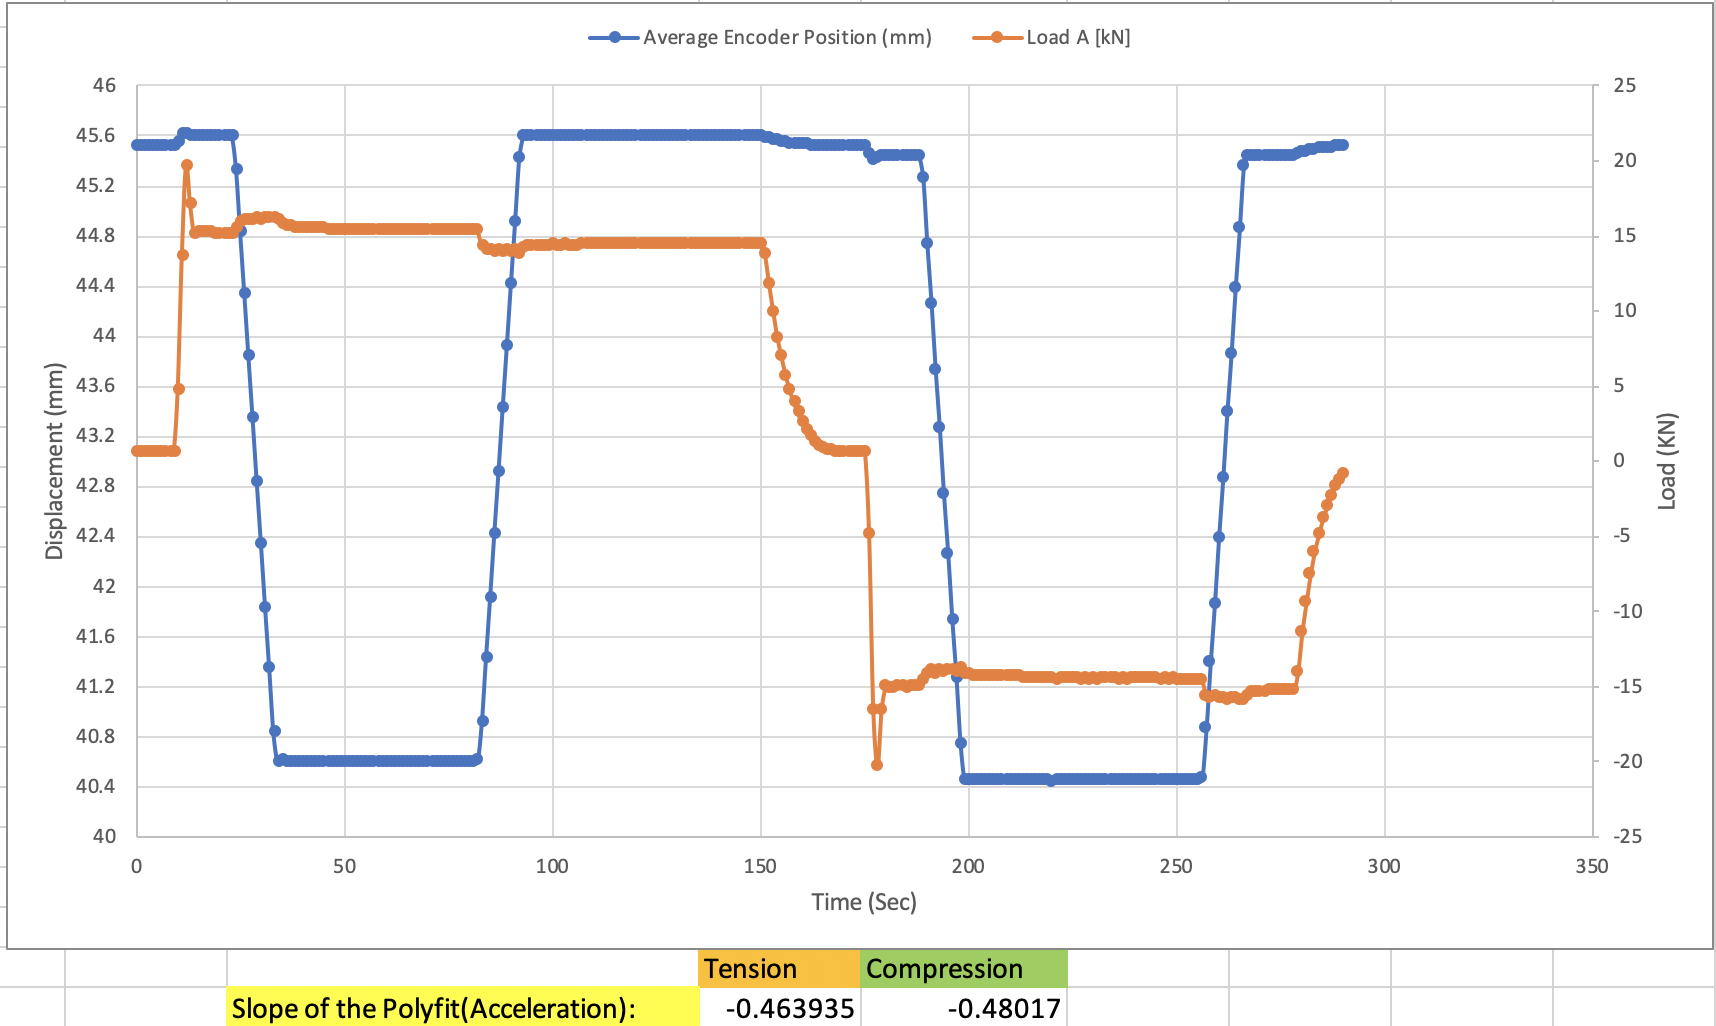
\includegraphics[width=5.98958in]{jira_imgs/4102.png}\\[2\baselineskip]After
Encoder A reached 40.386mm and Encoder B reached 40.803mm, it took about
1 second for the actuator to settle to within 0.001mm of that position.
In 1 second, Encoder A was seen to be 40.386mm and Encoder B was
40.804mm.

}
\begin{tabular}{p{2cm}p{14cm}}
\toprule
Step 14 & Step Execution Status: \textbf{ Pass } \\ \hline
\end{tabular}
 Description \\
{\footnotesize
Check if all the test results are recorded in excel spreadsheets.

}
\hdashrule[0.5ex]{\textwidth}{1pt}{3mm}
  Expected Result \\
{\footnotesize
Test Results are recorded in the excel spreadsheets residing in the
LabView Folder directory.

}
\hdashrule[0.5ex]{\textwidth}{1pt}{3mm}
  Actual Result \\
{\footnotesize
The excel file is attached to the execution of this test case.

}
\begin{tabular}{p{2cm}p{14cm}}
\toprule
Step 15 & Step Execution Status: \textbf{ Not Executed } \\ \hline
\end{tabular}
 Description \\
{\footnotesize
Close all the Labview VI files.

}
\hdashrule[0.5ex]{\textwidth}{1pt}{3mm}
  Test Data \\
 {\footnotesize
\textbf{Note:~}Labview can be left open in order to continue to the next
test. However, it may be necessary to reset the application before
starting the next test.

}
\hdashrule[0.5ex]{\textwidth}{1pt}{3mm}
  Expected Result \\
{\footnotesize
All the VI files are closed and Labview 2021 application window closes.

}
\hdashrule[0.5ex]{\textwidth}{1pt}{3mm}
  Actual Result \\
{\footnotesize
The LabView VI's were stopped, but not closed.

}

\paragraph{ LVV-T2432 - Hexapod - Actuator Range of Motion Test }\mbox{}\\

Version \textbf{1}.
Status \textbf{Approved}.
Open  \href{https://jira.lsstcorp.org/secure/Tests.jspa#/testCase/LVV-T2432}{\textit{ LVV-T2432 } }
test case in Jira.

To verify that the range of motions for the actuators stay within the
determined limits.

\textbf{ Preconditions}:\\
The range limits should be determined to achieve the camera hexapod's
simultaneous range of motion requirements.

Execution status: {\bf Pass }

Final comment:\\The purpose of this test was to verify that the limit switches would
prevent the actuator from moving beyond an unsafe range of motion. The
actuator can incur serious damage if allowed to move beyond +/-15mm.
Therefore, the limits switches were set to be around +/-14.3mm, which is
within the +/-15mm but capable of allowing the overall hexapod range of
motion requirements to still be met.\\
During the Modified Actuator Verification Campaign, a new set of limit
switches had to be installed. However, the paddles on the limit switches
were not bent exactly like the original limit switches. As a result, the
limit switches had to be manually readjusted to trigger as close as
possible to the original +/-14.3mm. The calculations that were used to
determine the necessary adjustment are seen in the attached document.\\
Overall, this test was considered to be passed as the limit switches
were readjusted and seen to stop the actuator from moving beyond its
range of motion. The full range of motion is listed below:\\
Negative Limit Switch:

\begin{itemize}
\tightlist
\item
  Copley Software: Active Load Position = \textbf{-36.03mm or
  -36003000counts}
\item
  Encoder A (D13B) = 53.28mm
\item
  Encoder B (D0BD) = 53.73mm
\end{itemize}

Zero Position:

\begin{itemize}
\tightlist
\item
  Copley Software: Active Load Position = \textbf{-22.008mm or -2200875
  counts}
\item
  Encoder A (D13B) = 39.4mm
\item
  Encoder B (D0BD) = 39.5mm
\end{itemize}

Positive Limit Switch:

\begin{itemize}
\tightlist
\item
  Copley Software: Active Load Position = \textbf{-7.515mm or
  -7515000counts}
\item
  Encoder A (D13B) = 24.78mm
\item
  Encoder B (D0BD) = 25.23mm
\end{itemize}

In conclusion, the stiffness of the actuator was seen in the following
positions as follows:

\begin{itemize}
\tightlist
\item
  Zero Position = 101.6N/um
\item
  Negative Limit Switch = 101.4N/um
\item
  Positive Limit Switch = 101.6N/um~
\end{itemize}

\href{https://docushare.lsst.org/docushare/dsweb/Services/Document-55106}{Encoder
Range Comparison (unmod vs mod).xlsx}


Detailed steps results:

\begin{tabular}{p{2cm}p{14cm}}
\toprule
Step 1 & Step Execution Status: \textbf{ Pass } \\ \hline
\end{tabular}
 Description \\
{\footnotesize
Open Labview 2021 in the computer used for Test Setup.

}
\hdashrule[0.5ex]{\textwidth}{1pt}{3mm}
  Test Data \\
 {\footnotesize
The first three steps are conditional because these steps are included
as part of the Test Setup procedure and may not be necessary if LabView
is still open.\\[3\baselineskip]

}
\hdashrule[0.5ex]{\textwidth}{1pt}{3mm}
  Expected Result \\
{\footnotesize
Labview 2021 opens successfully.

}
\hdashrule[0.5ex]{\textwidth}{1pt}{3mm}
  Actual Result \\
{\footnotesize
Labview was already open.

}
\begin{tabular}{p{2cm}p{14cm}}
\toprule
Step 2 & Step Execution Status: \textbf{ Pass } \\ \hline
\end{tabular}
 Description \\
{\footnotesize
Run the following VI's:

\begin{itemize}
\tightlist
\item
  Encoder A (D13B) and Load Cell.vi
\item
  Encoder B (D0BD).vi
\end{itemize}

}
\hdashrule[0.5ex]{\textwidth}{1pt}{3mm}
  Expected Result \\
{\footnotesize
Front panel of the VI's open without any error.

}
\hdashrule[0.5ex]{\textwidth}{1pt}{3mm}
  Actual Result \\
{\footnotesize
LabView and the required VI's were already opened at the start of the
execution of this test cycle.

}
\begin{tabular}{p{2cm}p{14cm}}
\toprule
Step 3 & Step Execution Status: \textbf{ Pass } \\ \hline
\end{tabular}
 Description \\
{\footnotesize
Click Run button on the block diagram toolbar of the Labview VI front
panel.

}
\hdashrule[0.5ex]{\textwidth}{1pt}{3mm}
  Expected Result \\
{\footnotesize
LabView VI and associated sub Vi runs successfully. The graphs should
start to be populated with data once the run button is pressed.

}
\hdashrule[0.5ex]{\textwidth}{1pt}{3mm}
  Actual Result \\
{\footnotesize
LabView was ran without any issue.

}
\begin{tabular}{p{2cm}p{14cm}}
\toprule
Step 4 & Step Execution Status: \textbf{ Fail } \\ \hline
\end{tabular}
 Description \\
{\footnotesize
Set software actuator stroke limits using the copley software to +/-
14.00mm.

}
\hdashrule[0.5ex]{\textwidth}{1pt}{3mm}
  Expected Result \\
{\footnotesize
Software actuator stroke limits set to +/- 14.00mm.

}
\hdashrule[0.5ex]{\textwidth}{1pt}{3mm}
  Actual Result \\
{\footnotesize
As seen during the Unmodified Actuator Verification Campaign, the
software limits were not able to be set.

}
\begin{tabular}{p{2cm}p{14cm}}
\toprule
Step 5 & Step Execution Status: \textbf{ Pass } \\ \hline
\end{tabular}
 Description \\
{\footnotesize
Move the actuator forward and backward to confirm that positive position
commands correspond to extensions of the actuator and negative position
commands correspond to retractions of the actuator. If not, flipped the
sign of the encoder readings in software.~\\[2\baselineskip]

}
\hdashrule[0.5ex]{\textwidth}{1pt}{3mm}
  Expected Result \\
{\footnotesize
Positive position commands correspond to extensions; Negative position
commands correspond to retractions of the actuator.~

}
\hdashrule[0.5ex]{\textwidth}{1pt}{3mm}
  Actual Result \\
{\footnotesize
New limit switches were installed and it was confirmed that to the
farthest positive position triggered the positive limit switch and
moving to the farthest negative position triggered the negative limit
switch.~

}
\begin{tabular}{p{2cm}p{14cm}}
\toprule
Step 6 & Step Execution Status: \textbf{ Pass } \\ \hline
\end{tabular}
 Description \\
{\footnotesize
Set the motor drive to halt motion using the control box and copley
software if a limit switch is tripped.\\[3\baselineskip]

}
\hdashrule[0.5ex]{\textwidth}{1pt}{3mm}
  Expected Result \\
{\footnotesize
Motor drive set to halt position if a limit switch is tripped.~

}
\hdashrule[0.5ex]{\textwidth}{1pt}{3mm}
  Actual Result \\
{\footnotesize
The actuator was confirmed to stop once it tripped a limit switch. The
software would display the fault and no motion could be commanded
further into the limit switch.

}
\begin{tabular}{p{2cm}p{14cm}}
\toprule
Step 7 & Step Execution Status: \textbf{ Fail } \\ \hline
\end{tabular}
 Description \\
{\footnotesize
Extend the actuator to its position stroke limit of +14mm using the
copley software and the~ control box.

}
\hdashrule[0.5ex]{\textwidth}{1pt}{3mm}
  Expected Result \\
{\footnotesize
Actuator extended to its position stroke limit of +14mm.

}
\hdashrule[0.5ex]{\textwidth}{1pt}{3mm}
  Actual Result \\
{\footnotesize
During MOOG's original testing, they used a separate software that
allowed them to set/change the software limits of the actuator. Instead,
the position of the limit switches were simply verified without setting
the software limits. Since the software limits were not set, this step
is marked as Fail.

}
\begin{tabular}{p{2cm}p{14cm}}
\toprule
Step 8 & Step Execution Status: \textbf{ Not Executed } \\ \hline
\end{tabular}
 Description \\
{\footnotesize
Ensure that the actuator reaches this position without hitting the
mechanical end stop or extension limit switch.

}
\hdashrule[0.5ex]{\textwidth}{1pt}{3mm}
  Expected Result \\
{\footnotesize
Encoder reading in LabView shows that actuator reached the position.~\\
Mechanical End Stop/Extension Limit switch not hit.

}
\hdashrule[0.5ex]{\textwidth}{1pt}{3mm}
  Actual Result \\
{\footnotesize
As mentioned in the previous step, since the software limits of the
actuator could not be set/changed, this step was not executed.

}
\begin{tabular}{p{2cm}p{14cm}}
\toprule
Step 9 & Step Execution Status: \textbf{ Not Executed } \\ \hline
\end{tabular}
 Description \\
{\footnotesize
If the extension limit switch is contacted, the extension limit switch
position will need to be adjusted to be greater than 14mm and then the
try to extend the actuator to the position stroke limit of +14mm using
copley software and the control box.

}
\hdashrule[0.5ex]{\textwidth}{1pt}{3mm}
  Expected Result \\
{\footnotesize
Extension Limit Switch position readjusted and extended to the position
stroke limit of +14mm.

}
\hdashrule[0.5ex]{\textwidth}{1pt}{3mm}
  Actual Result \\
{\footnotesize
Again, since the software limits of the actuator could not be
set/changed, this step was not executed. Furthermore, this step was
conditional.

}
\begin{tabular}{p{2cm}p{14cm}}
\toprule
Step 10 & Step Execution Status: \textbf{ Not Executed } \\ \hline
\end{tabular}
 Description \\
{\footnotesize
Ensure that the actuator reaches this position without hitting the
mechanical end stop or extension limit switch.

}
\hdashrule[0.5ex]{\textwidth}{1pt}{3mm}
  Expected Result \\
{\footnotesize
Encoder reading in LabView shows that actuator reached the position.\\
Mechanical End Stop/Extension Limit switch not hit.

}
\hdashrule[0.5ex]{\textwidth}{1pt}{3mm}
  Actual Result \\
{\footnotesize
Again, since the software limits of the actuator could not be
set/changed, this step was not executed. Furthermore, this step was
conditional.

}
\begin{tabular}{p{2cm}p{14cm}}
\toprule
Step 11 & Step Execution Status: \textbf{ Not Executed } \\ \hline
\end{tabular}
 Description \\
{\footnotesize
Move the extension actuator stroke limit using the copley software to
+15.00mm .

}
\hdashrule[0.5ex]{\textwidth}{1pt}{3mm}
  Expected Result \\
{\footnotesize
Extension actuator stroke limit moved to +15.00mm.~

}
\hdashrule[0.5ex]{\textwidth}{1pt}{3mm}
  Actual Result \\
{\footnotesize
As mentioned in the previous step, since the software limits of the
actuator could not be set/changed, this step was not executed.

}
\begin{tabular}{p{2cm}p{14cm}}
\toprule
Step 12 & Step Execution Status: \textbf{ Pass } \\ \hline
\end{tabular}
 Description \\
{\footnotesize
Extend the actuator at maximum velocity until the extension limit switch
is actuated.

}
\hdashrule[0.5ex]{\textwidth}{1pt}{3mm}
  Test Data \\
 {\footnotesize
\textbf{Note:~}The maximum velocity is +/-0.5mm/s

}
\hdashrule[0.5ex]{\textwidth}{1pt}{3mm}
  Expected Result \\
{\footnotesize
Actuator extended at maximum velocity until the extension limit switch
is actuated.~

}
\hdashrule[0.5ex]{\textwidth}{1pt}{3mm}
  Actual Result \\
{\footnotesize
The maximum velocity on the Copley control software was set to 0.5mm/s
by default. The actuator was commanded to about +14mm initially and then
in increments of +0.1mm until the limit switch was triggered. As a
result, the limit switch was seen to be triggered at +14.3mm.

}
\begin{tabular}{p{2cm}p{14cm}}
\toprule
Step 13 & Step Execution Status: \textbf{ Not Executed } \\ \hline
\end{tabular}
 Description \\
{\footnotesize
If the actuator hits the stroke limit before tripping the limit switch
or appears to contact the end stop after tripping the limit switch
(before it can stop), reposition the limit switch. Then, repeat test
using copley software and the control box.\\[2\baselineskip]

}
\hdashrule[0.5ex]{\textwidth}{1pt}{3mm}
  Expected Result \\
{\footnotesize
Limit switch repositioned and extended the actuator to the position
stroke limit of +15mm.~

}
\hdashrule[0.5ex]{\textwidth}{1pt}{3mm}
  Actual Result \\
{\footnotesize
During MOOG's original testing, they used a separate software that
allowed them to set the stroke limits of the actuator. Instead, the
position of the limit switches were simply verified without using
software limits. Since this does not impact the results of our tests,
this step was skipped.

}
\begin{tabular}{p{2cm}p{14cm}}
\toprule
Step 14 & Step Execution Status: \textbf{ Pass } \\ \hline
\end{tabular}
 Description \\
{\footnotesize
Record the final position of the limit switch.~\\[2\baselineskip]

}
\hdashrule[0.5ex]{\textwidth}{1pt}{3mm}
  Expected Result \\
{\footnotesize
Final position of the limit switch is around +14.50mm.

}
\hdashrule[0.5ex]{\textwidth}{1pt}{3mm}
  Actual Result \\
{\footnotesize
During the Unmodified Actuator Verification Campaign, the limit switch
positions were seen to be +/-14.298. During this test, new limit
switches were installed and had to be manually adjusted so that they
were as close to the original limit switch positions as possible. As a
result the positive limit switch was seen to be +14.3mm

}
\begin{tabular}{p{2cm}p{14cm}}
\toprule
Step 15 & Step Execution Status: \textbf{ Not Executed } \\ \hline
\end{tabular}
 Description \\
{\footnotesize
Repeat the steps 6-14 two more times to assess limit switch position
repeatability. ~\\[3\baselineskip]

}
\hdashrule[0.5ex]{\textwidth}{1pt}{3mm}
  Expected Result \\
{\footnotesize
Final positions of the limit switch close to step 14 result(Around
+14.50).

}
\hdashrule[0.5ex]{\textwidth}{1pt}{3mm}
  Actual Result \\
{\footnotesize
The limit switch was seen to be roughly around +14.298mm as recorded in
step 14 when repeated once more. However, this step was skipped as we
didn't want to cause hysteresis in the paddle for the limit switch.

}
\begin{tabular}{p{2cm}p{14cm}}
\toprule
Step 16 & Step Execution Status: \textbf{ Fail } \\ \hline
\end{tabular}
 Description \\
{\footnotesize
Retract the actuator to its position stroke limit of -14 mm using the
copley software and the ~control box.\\[2\baselineskip]

}
\hdashrule[0.5ex]{\textwidth}{1pt}{3mm}
  Expected Result \\
{\footnotesize
Actuator retracted to its position stroke limit of -14.04mm.

}
\hdashrule[0.5ex]{\textwidth}{1pt}{3mm}
  Actual Result \\
{\footnotesize
During MOOG's original testing, they used a separate software that
allowed them to set/change the software limits of the actuator. Instead,
the position of the limit switches were simply verified without setting
the software limits. Since the software limits were not set, this step
is marked as Fail.

}
\begin{tabular}{p{2cm}p{14cm}}
\toprule
Step 17 & Step Execution Status: \textbf{ Not Executed } \\ \hline
\end{tabular}
 Description \\
{\footnotesize
Ensure that the actuator reaches this position without hitting the
mechanical end stop or retraction limit switch.

}
\hdashrule[0.5ex]{\textwidth}{1pt}{3mm}
  Expected Result \\
{\footnotesize
Encoder reading in LabView shows that actuator reached the position.\\
Mechanical End Stop/Retraction Limit switch not hit.

}
\hdashrule[0.5ex]{\textwidth}{1pt}{3mm}
  Actual Result \\
{\footnotesize
As mentioned in the previous step, since the software limits of the
actuator could not be set/changed, this step was not executed.

}
\begin{tabular}{p{2cm}p{14cm}}
\toprule
Step 18 & Step Execution Status: \textbf{ Not Executed } \\ \hline
\end{tabular}
 Description \\
{\footnotesize
If the retraction limit switch is contacted, the retraction limit switch
position will need to be adjusted to be greater than -14mm and then the
try to retract the actuator to the position stroke limit of -14mm using
copley software and the control box.

}
\hdashrule[0.5ex]{\textwidth}{1pt}{3mm}
  Expected Result \\
{\footnotesize
Retraction limit switch position readjusted and the actuator retracted
to the position stroke limit of -14mm.

}
\hdashrule[0.5ex]{\textwidth}{1pt}{3mm}
  Actual Result \\
{\footnotesize
Again, since the software limits of the actuator could not be
set/changed, this step was not executed. Furthermore, this step was
conditional.

}
\begin{tabular}{p{2cm}p{14cm}}
\toprule
Step 19 & Step Execution Status: \textbf{ Not Executed } \\ \hline
\end{tabular}
 Description \\
{\footnotesize
Ensure that the actuator reaches this position without hitting the
mechanical end stop or retraction limit switch.

}
\hdashrule[0.5ex]{\textwidth}{1pt}{3mm}
  Expected Result \\
{\footnotesize
Encoder reading in LabView shows that actuator reached the position.\\
Mechanical End Stop/Retraction Limit switch not hit.

}
\hdashrule[0.5ex]{\textwidth}{1pt}{3mm}
  Actual Result \\
{\footnotesize
Again, since the software limits of the actuator could not be
set/changed, this step was not executed. Furthermore, this step was
conditional.

}
\begin{tabular}{p{2cm}p{14cm}}
\toprule
Step 20 & Step Execution Status: \textbf{ Not Executed } \\ \hline
\end{tabular}
 Description \\
{\footnotesize
Move the retraction actuator stroke limit to -15.00mm .~

}
\hdashrule[0.5ex]{\textwidth}{1pt}{3mm}
  Expected Result \\
{\footnotesize
Retraction actuator stroke limit moved to -15.00mm.

}
\hdashrule[0.5ex]{\textwidth}{1pt}{3mm}
  Actual Result \\
{\footnotesize
As mentioned in the previous step, since the software limits of the
actuator could not be set/changed, this step was not executed.

}
\begin{tabular}{p{2cm}p{14cm}}
\toprule
Step 21 & Step Execution Status: \textbf{ Pass } \\ \hline
\end{tabular}
 Description \\
{\footnotesize
Retract the actuator at maximum velocity until the retraction limit
switch is actuated.

}
\hdashrule[0.5ex]{\textwidth}{1pt}{3mm}
  Test Data \\
 {\footnotesize
\textbf{Note:~}The maximum velocity is +/-0.5mm/s

}
\hdashrule[0.5ex]{\textwidth}{1pt}{3mm}
  Expected Result \\
{\footnotesize
Actuator retracted at maximum velocity until the retraction limit switch
is actuated.

}
\hdashrule[0.5ex]{\textwidth}{1pt}{3mm}
  Actual Result \\
{\footnotesize
The maximum velocity on the Copley control software was set to 0.5mm/s
by default. The actuator was commanded to about -14mm initially and then
in increments of -0.1mm until the limit switch was triggered. As a
result, the limit switch was seen to be triggered at -14.3mm.

}
\begin{tabular}{p{2cm}p{14cm}}
\toprule
Step 22 & Step Execution Status: \textbf{ Not Executed } \\ \hline
\end{tabular}
 Description \\
{\footnotesize
If the actuator hits the stroke limit before tripping the limit switch
or appears to contact the end stop after tripping the limit switch
(before it can stop), reposition the limit switch and repeat test.

}
\hdashrule[0.5ex]{\textwidth}{1pt}{3mm}
  Expected Result \\
{\footnotesize
Limit switch repositioned and retracted the actuator to the position
stroke limit of -15mm.

}
\hdashrule[0.5ex]{\textwidth}{1pt}{3mm}
  Actual Result \\
{\footnotesize
During MOOG's original testing, they used a separate software that
allowed them to set the software limits of the actuator. Instead, the
position of the limit switches were simply verified without using
software limits. Since this does not impact the results of our tests,
this step was skipped.

}
\begin{tabular}{p{2cm}p{14cm}}
\toprule
Step 23 & Step Execution Status: \textbf{ Pass } \\ \hline
\end{tabular}
 Description \\
{\footnotesize
Record the final position of the limit switch.

}
\hdashrule[0.5ex]{\textwidth}{1pt}{3mm}
  Expected Result \\
{\footnotesize
Final position of the limit switch is around -14.50mm.

}
\hdashrule[0.5ex]{\textwidth}{1pt}{3mm}
  Actual Result \\
{\footnotesize
During the Unmodified Actuator Verification Campaign, the limit switch
positions were seen to be +/-14.298. During this test, new limit
switches were installed and had to be manually adjusted so that they
were as close to the original limit switch positions as possible. As a
result the positive limit switch was seen to be -14.3mm

}
\begin{tabular}{p{2cm}p{14cm}}
\toprule
Step 24 & Step Execution Status: \textbf{ Not Executed } \\ \hline
\end{tabular}
 Description \\
{\footnotesize
Repeat the steps 16-23 two more times to assess limit switch position
repeatability.

}
\hdashrule[0.5ex]{\textwidth}{1pt}{3mm}
  Expected Result \\
{\footnotesize
Final positions of the limit switch close to step 15 result(Around
-14.50).

}
\hdashrule[0.5ex]{\textwidth}{1pt}{3mm}
  Actual Result \\
{\footnotesize
The limit switch was seen to be roughly around -14.3mm as recorded in
step 23 when repeated once more. However, this step was skipped as we
didn't want to cause hysteresis in the paddle for the limit switch.

}
\begin{tabular}{p{2cm}p{14cm}}
\toprule
Step 25 & Step Execution Status: \textbf{ Pass } \\ \hline
\end{tabular}
 Description \\
{\footnotesize
Check if all the test results are recorded in excel spreadsheets.

}
\hdashrule[0.5ex]{\textwidth}{1pt}{3mm}
  Expected Result \\
{\footnotesize
Test Results are recorded in the excel spreadsheets residing in the
LabView Folder directory.\\[2\baselineskip]

}
\hdashrule[0.5ex]{\textwidth}{1pt}{3mm}
  Actual Result \\
{\footnotesize
The results and calculations from this test can be found in the
attached~\emph{Encoder Range Comparison (unmod vs mod).xlsx.}

}
\begin{tabular}{p{2cm}p{14cm}}
\toprule
Step 26 & Step Execution Status: \textbf{ Not Executed } \\ \hline
\end{tabular}
 Description \\
{\footnotesize
Close the Labview Vi file.

}
\hdashrule[0.5ex]{\textwidth}{1pt}{3mm}
  Test Data \\
 {\footnotesize
\textbf{Note:~}Labview can be left open in order to continue to the next
test. However, it may be necessary to reset the application before
starting the next test.

}
\hdashrule[0.5ex]{\textwidth}{1pt}{3mm}
  Expected Result \\
{\footnotesize
Labview 2021 application window closes.

}
\hdashrule[0.5ex]{\textwidth}{1pt}{3mm}
  Actual Result \\
{\footnotesize
The LabView VI's were stopped, but not closed.

}

\paragraph{ LVV-T2434 - Hexapod - Actuator Resolution Test }\mbox{}\\

Version \textbf{1}.
Status \textbf{Approved}.
Open  \href{https://jira.lsstcorp.org/secure/Tests.jspa#/testCase/LVV-T2434}{\textit{ LVV-T2434 } }
test case in Jira.



\textbf{ Preconditions}:\\
This test can be performed at any starting position within the
actuator's range of motion that allow the test to be completed without
exceeding the software range limits. It is preferable to use different
starting positions for different actuators although no performance
deviations are expected.~\\[2\baselineskip]

Execution status: {\bf Pass }

Final comment:\\The expected result of this test was that given 100nm moves with any
load, the actuator would reach the commanded position within 50nm.
However, there were some deviations to the 100nm moves seen to be
greater than 50nm. This was expected as MOOG's original test results
described similar issues related to excessive noise on the load cell and
on the external encoders. Additionally, a load compensation could not be
performed with the displacement being measured in nm's. Therefore, since
the encoders were seen to be able to track the actuator movement closely
and in the correct commanded direction, this test was passed.


Detailed steps results:

\begin{tabular}{p{2cm}p{14cm}}
\toprule
Step 1 & Step Execution Status: \textbf{ Pass } \\ \hline
\end{tabular}
 Description \\
{\footnotesize
Open Labview 2021 in the computer used for Test Setup.~

}
\hdashrule[0.5ex]{\textwidth}{1pt}{3mm}
  Test Data \\
 {\footnotesize
The first three steps are conditional because these steps are included
as part of the Test Setup procedure and may not be necessary if LabView
is still open.

}
\hdashrule[0.5ex]{\textwidth}{1pt}{3mm}
  Expected Result \\
{\footnotesize
Labview 2021 opens successfully.~

}
\hdashrule[0.5ex]{\textwidth}{1pt}{3mm}
  Actual Result \\
{\footnotesize
Labview was opened successfully.

}
\begin{tabular}{p{2cm}p{14cm}}
\toprule
Step 2 & Step Execution Status: \textbf{ Pass } \\ \hline
\end{tabular}
 Description \\
{\footnotesize
Run the following VI's:

\begin{itemize}
\tightlist
\item
  Encoder A (D13B) and Load Cell.vi
\item
  Encoder B (D0BD).vi
\end{itemize}

}
\hdashrule[0.5ex]{\textwidth}{1pt}{3mm}
  Expected Result \\
{\footnotesize
Front panel of VI's open without any error.

}
\hdashrule[0.5ex]{\textwidth}{1pt}{3mm}
  Actual Result \\
{\footnotesize
LabView and the required VI's were already opened at the start of the
execution of this test cycle.

}
\begin{tabular}{p{2cm}p{14cm}}
\toprule
Step 3 & Step Execution Status: \textbf{ Pass } \\ \hline
\end{tabular}
 Description \\
{\footnotesize
Click Run button on the block diagram toolbar of the Labview VI front
panel.

}
\hdashrule[0.5ex]{\textwidth}{1pt}{3mm}
  Expected Result \\
{\footnotesize
LabView VI and associated sub Vi runs successfully. The graphs should
start to be populated with data once the run button is pressed.

}
\hdashrule[0.5ex]{\textwidth}{1pt}{3mm}
  Actual Result \\
{\footnotesize
The actuator was in the following position at the start of the test:\\

\begin{itemize}
\tightlist
\item
  Copley Software: Active Load Position = \textbf{-22.98mm or
  -22980000counts}
\item
  Encoder A (D13B) = 39.34mm
\item
  Encoder B (D0BD) = 39.77mm
\end{itemize}

}
\begin{tabular}{p{2cm}p{14cm}}
\toprule
Step 4 & Step Execution Status: \textbf{ Pass } \\ \hline
\end{tabular}
 Description \\
{\footnotesize
Apply a force of +15kN.

}
\hdashrule[0.5ex]{\textwidth}{1pt}{3mm}
  Test Data \\
 {\footnotesize
\textbf{Note:~}In order to apply a tension force of +15 kN, set Channel
1 = 2.19V and Channel 0 = 0V.~

}
\hdashrule[0.5ex]{\textwidth}{1pt}{3mm}
  Expected Result \\
{\footnotesize
Load cell reader shows the applied +15 KN \textbf{tension} force.\\
LabView displays the voltage being applied.

}
\hdashrule[0.5ex]{\textwidth}{1pt}{3mm}
  Actual Result \\
{\footnotesize
+15kN by setting Channel 1 = 4.38

}
\begin{tabular}{p{2cm}p{14cm}}
\toprule
Step 5 & Step Execution Status: \textbf{ Pass } \\ \hline
\end{tabular}
 Description \\
{\footnotesize
Record the load cell value in the LabView in the form of Load vs Time
graph.~

}
\hdashrule[0.5ex]{\textwidth}{1pt}{3mm}
  Expected Result \\
{\footnotesize
LabView load graph (Load vs Time) shows +15 kN tension force applied.~

}
\hdashrule[0.5ex]{\textwidth}{1pt}{3mm}
  Actual Result \\
{\footnotesize
The values measuring the load were exported from LabView into the
Tension sheet of the
\href{https://docushare.lsst.org/docushare/dsweb/Services/Document-55069}{\emph{Resolution
Test Results - Modified Actuator.xlsx~}}excel document. The applied load
during this test can be seen as the orange line in the plot below:\\
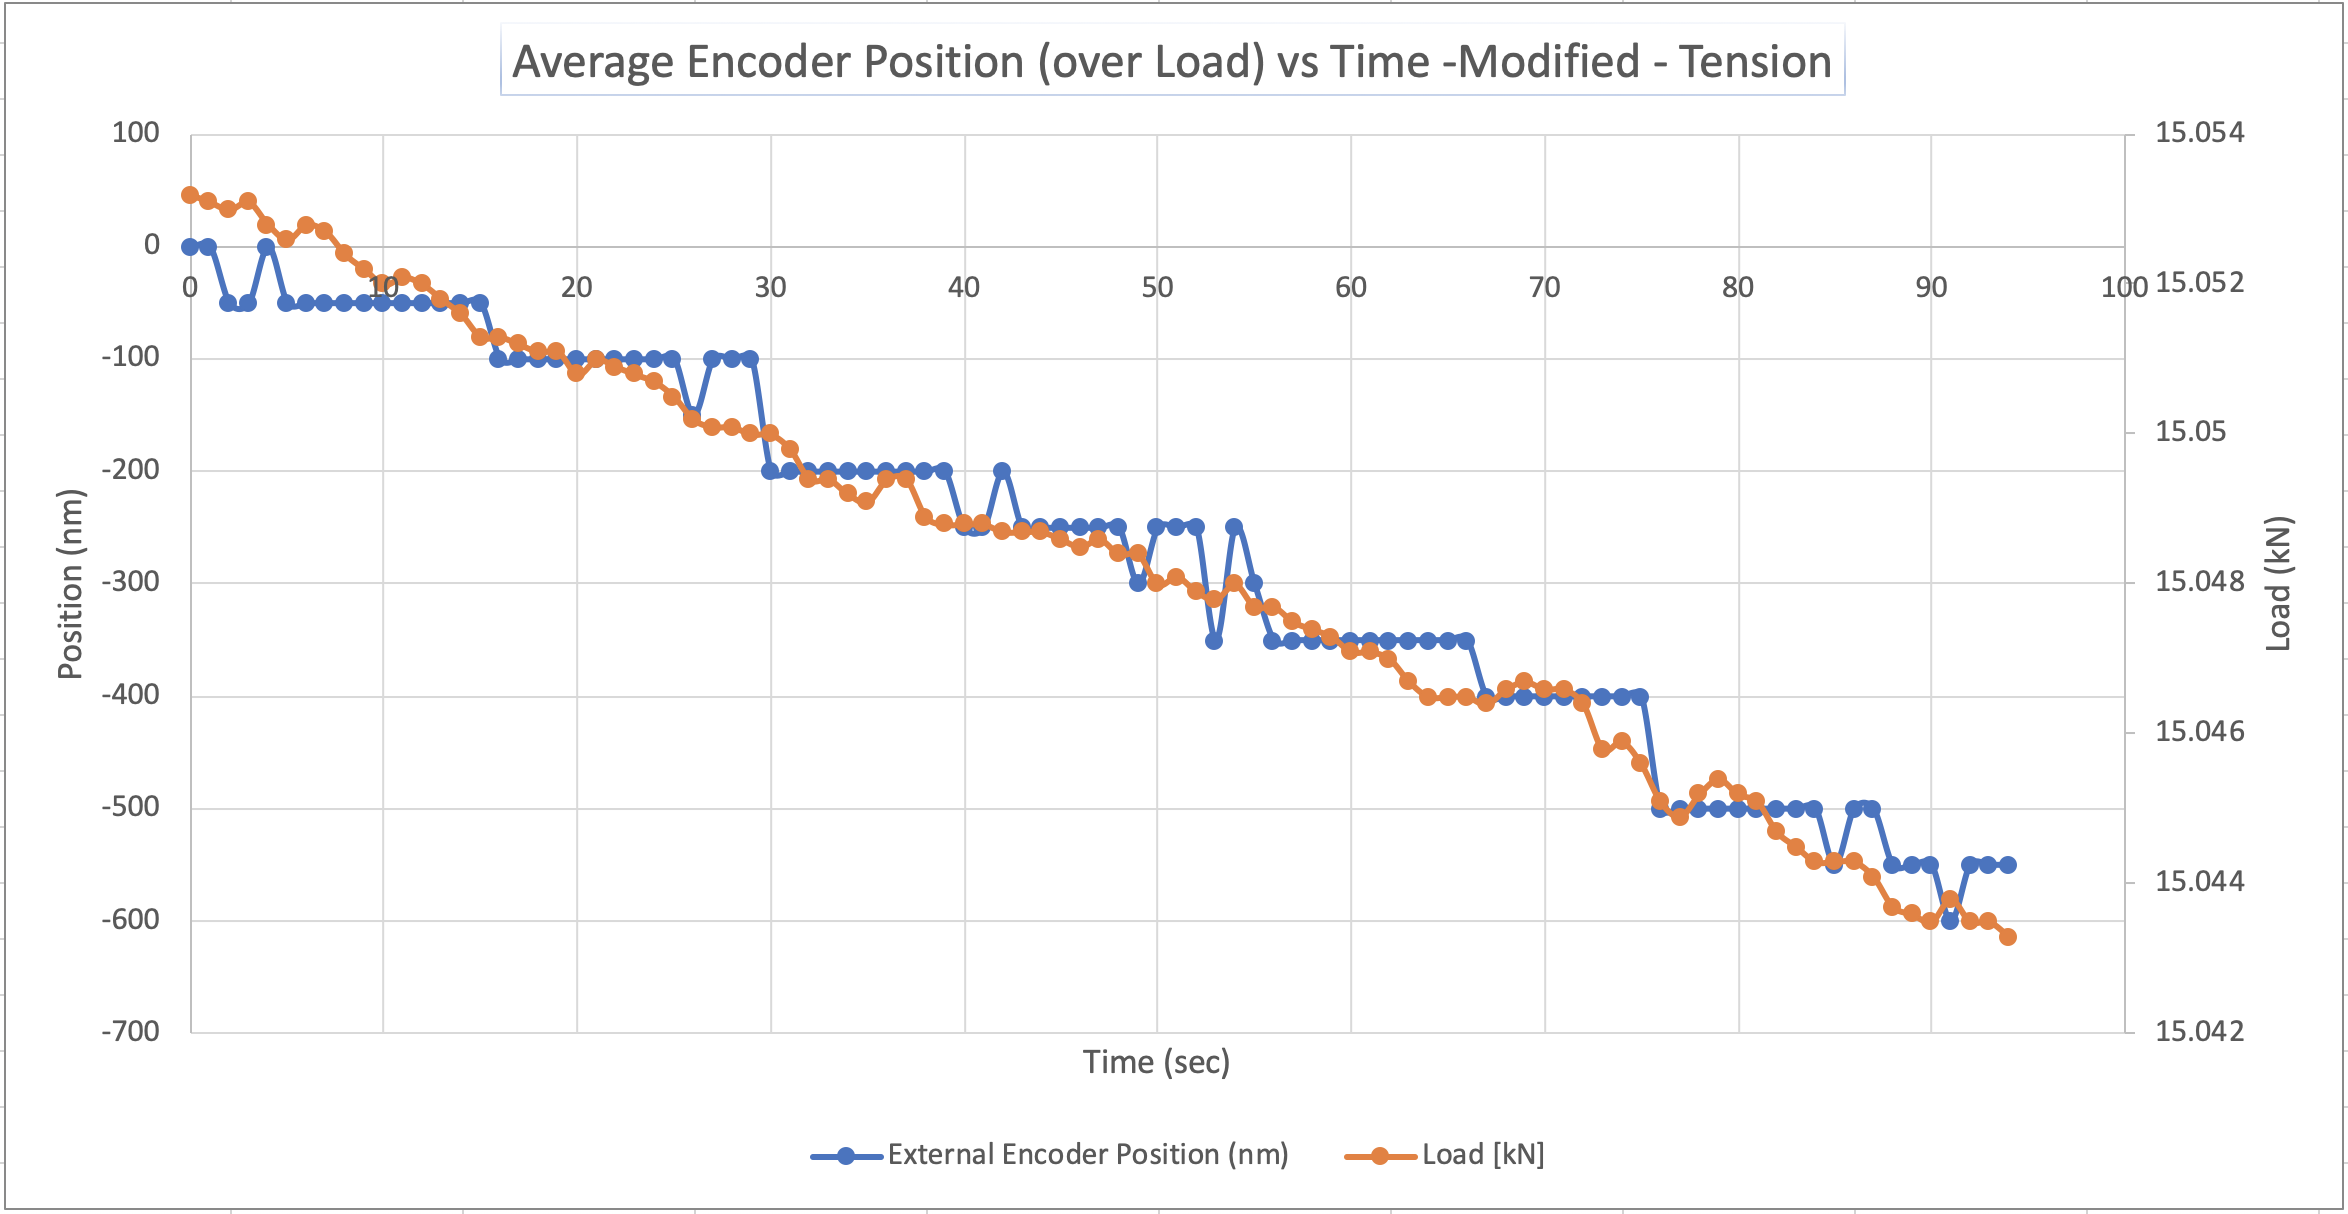
\includegraphics[width=5.98958in]{jira_imgs/4108.png}

}
\begin{tabular}{p{2cm}p{14cm}}
\toprule
Step 6 & Step Execution Status: \textbf{ Pass } \\ \hline
\end{tabular}
 Description \\
{\footnotesize
Execute the following commands to the actuator in relative positioning
mode using the copley software and the control box : extend 100nm,
extend 100nm, extend 100nm, retract 100nm, extend 100nm, retract 100nm,
retract 100nm, retract 100nm.\\[2\baselineskip]

}
\hdashrule[0.5ex]{\textwidth}{1pt}{3mm}
  Test Data \\
 {\footnotesize
\textbf{Note:~}Take note of the time at which the moves are commanded.
It will be difficult to determine when the series of commands are sent
because the moves are so small.

}
\hdashrule[0.5ex]{\textwidth}{1pt}{3mm}
  Expected Result \\
{\footnotesize
All moves should move in the commanded directions.~

}
\hdashrule[0.5ex]{\textwidth}{1pt}{3mm}
  Actual Result \\
{\footnotesize
Starting at the center position,\\[2\baselineskip]Moved +100nm
(11:37:31)\\[2\baselineskip]Moved +100nm
(11:37:38)\\[2\baselineskip]Moved +100nm
(11:37:44)\\[2\baselineskip]Moved -100nm
(11:37:52)\\[2\baselineskip]Moved +100nm
(11:38:01)\\[2\baselineskip]Moved -100nm
(11:38:07)\\[2\baselineskip]Moved -100nm
(11:38:16)\\[2\baselineskip]Moved -100nm
(11:38:23)\\[2\baselineskip]These are consistent to the timestamps taken
in the Tension sheet of the attached \emph{Resolution Test Results -
Modified Actuator.xlsx~}excel document

}
\begin{tabular}{p{2cm}p{14cm}}
\toprule
Step 7 & Step Execution Status: \textbf{ Pass } \\ \hline
\end{tabular}
 Description \\
{\footnotesize
Record the actual displacement as measured by the two external encoders
as LabView graph (Displacement vs Time).

}
\hdashrule[0.5ex]{\textwidth}{1pt}{3mm}
  Expected Result \\
{\footnotesize
Actual displacement measured by the average of the two external encoders
~recorded in the LabView graph.~

}
\hdashrule[0.5ex]{\textwidth}{1pt}{3mm}
  Actual Result \\
{\footnotesize
The displacement can be seen as the blue line in the plot attached to
the result of Step 5.

}
\begin{tabular}{p{2cm}p{14cm}}
\toprule
Step 8 & Step Execution Status: \textbf{ Pass } \\ \hline
\end{tabular}
 Description \\
{\footnotesize
Record the actual displacement as measured by the internal encoder using
copley software.~

}
\hdashrule[0.5ex]{\textwidth}{1pt}{3mm}
  Expected Result \\
{\footnotesize
Actual displacement measured by the internal encoder recorded in the
Copley Software.

}
\hdashrule[0.5ex]{\textwidth}{1pt}{3mm}
  Actual Result \\
{\footnotesize
The Active Load Position reported by the Copley Control Software could
not be exported. However, we confirmed after every move that the
relative motion moved +/-100nm each command.

}
\begin{tabular}{p{2cm}p{14cm}}
\toprule
Step 9 & Step Execution Status: \textbf{ Pass } \\ \hline
\end{tabular}
 Description \\
{\footnotesize
Ensure that the load cell signal did not vary significantly during the
test which would introduce compliance errors.

}
\hdashrule[0.5ex]{\textwidth}{1pt}{3mm}
  Expected Result \\
{\footnotesize
The tension load should remain close to 15kN throughout the displacement
movements and display in the Load vs Time graph in LabView.~

}
\hdashrule[0.5ex]{\textwidth}{1pt}{3mm}
  Actual Result \\
{\footnotesize
The load was seen to be consistent to 15.0kN as seen in the plot
attached to the result of Step 5.~

}
\begin{tabular}{p{2cm}p{14cm}}
\toprule
Step 10 & Step Execution Status: \textbf{ Pass } \\ \hline
\end{tabular}
 Description \\
{\footnotesize
Remove the 15 kN tension load.

}
\hdashrule[0.5ex]{\textwidth}{1pt}{3mm}
  Test Data \\
 {\footnotesize
\textbf{Note:~}Set Channel 0 = Channel 1 = 0V.

}
\hdashrule[0.5ex]{\textwidth}{1pt}{3mm}
  Expected Result \\
{\footnotesize
Load cell reader and Load graph in the LabView showing zero
load.\\[2\baselineskip]

}
\hdashrule[0.5ex]{\textwidth}{1pt}{3mm}
  Actual Result \\
{\footnotesize
Load was removed.

}
\begin{tabular}{p{2cm}p{14cm}}
\toprule
Step 11 & Step Execution Status: \textbf{ Pass } \\ \hline
\end{tabular}
 Description \\
{\footnotesize
Compare the internal linear encoder measurement with the average of the
two external linear encoder measurements.~

}
\hdashrule[0.5ex]{\textwidth}{1pt}{3mm}
  Expected Result \\
{\footnotesize
The magnitude should not vary by more than 50\% from the commanded value
based on an average of the two external linear encoder measurements.

}
\hdashrule[0.5ex]{\textwidth}{1pt}{3mm}
  Actual Result \\
{\footnotesize
The average displacement did not vary by more than 50nm during a
majority of the sequence of moves. However, there were some instances
where the measured displacement was seen to be
100nm.\\[2\baselineskip]This can be seen in column L of the Tension
sheet in the \emph{Resolution Test Results - Modified
Actuator.xlsx~}excel document.

}
\begin{tabular}{p{2cm}p{14cm}}
\toprule
Step 12 & Step Execution Status: \textbf{ Pass } \\ \hline
\end{tabular}
 Description \\
{\footnotesize
Apply a -15kN force.

}
\hdashrule[0.5ex]{\textwidth}{1pt}{3mm}
  Test Data \\
 {\footnotesize
\textbf{Note:~}In order to apply a compression force of -15 kN, set
Channel 0 = 2.19V and Channel 1 = 0V.

}
\hdashrule[0.5ex]{\textwidth}{1pt}{3mm}
  Expected Result \\
{\footnotesize
Load cell reader shows the applied -15 KN \textbf{compression} force.\\
LabView displays the voltage being applied.

}
\hdashrule[0.5ex]{\textwidth}{1pt}{3mm}
  Actual Result \\
{\footnotesize
The compression load of -15kN was applied.

}
\begin{tabular}{p{2cm}p{14cm}}
\toprule
Step 13 & Step Execution Status: \textbf{ Pass } \\ \hline
\end{tabular}
 Description \\
{\footnotesize
Execute the following commands to the actuator in relative positioning
mode using the copley software and the control box: extend 100nm, extend
100nm, extend 100nm, retract 100nm, extend 100nm, retract 100nm, retract
100nm, retract 100nm.\\[2\baselineskip]

}
\hdashrule[0.5ex]{\textwidth}{1pt}{3mm}
  Test Data \\
 {\footnotesize
\textbf{Note:~}Take note of the time at which the moves are commanded.
It will be difficult to determine when the series of commands are sent
because the moves are so small.

}
\hdashrule[0.5ex]{\textwidth}{1pt}{3mm}
  Expected Result \\
{\footnotesize
All moves should move in the commanded direction.

}
\hdashrule[0.5ex]{\textwidth}{1pt}{3mm}
  Actual Result \\
{\footnotesize
Starting at the center position,\\[2\baselineskip]Moved +100nm
(11:42:32)\\[2\baselineskip]Moved +100nm
(11:42:40)\\[2\baselineskip]Moved +100nm
(11:42:45)\\[2\baselineskip]Moved -100nm
(11:42:53)\\[2\baselineskip]Moved +100nm
(11:42:58)\\[2\baselineskip]Moved -100nm
(11:43:05)\\[2\baselineskip]Moved -100nm
(11:43:11)\\[2\baselineskip]Moved -100nm
(11:43:15)\\[2\baselineskip]These are consistent to the timestamps taken
in the Compression sheet of the attached \emph{Resolution Test Results -
Modified Actuator.xlsx~}excel document

}
\begin{tabular}{p{2cm}p{14cm}}
\toprule
Step 14 & Step Execution Status: \textbf{ Pass } \\ \hline
\end{tabular}
 Description \\
{\footnotesize
Record the actual displacement as measured by average of ~the two
external encoder as Labview graph (Displacement vs. Time).

}
\hdashrule[0.5ex]{\textwidth}{1pt}{3mm}
  Expected Result \\
{\footnotesize
Actual displacement measured by the average of the two external encoders
~recorded in the LabView graph.

}
\hdashrule[0.5ex]{\textwidth}{1pt}{3mm}
  Actual Result \\
{\footnotesize
The values measuring the load were exported from LabView into the
Compression sheet of the \emph{Resolution Test Results - Modified
Actuator.xlsx~}excel document.The applied load during this test can be
seen as the orange line in the plot below:\\
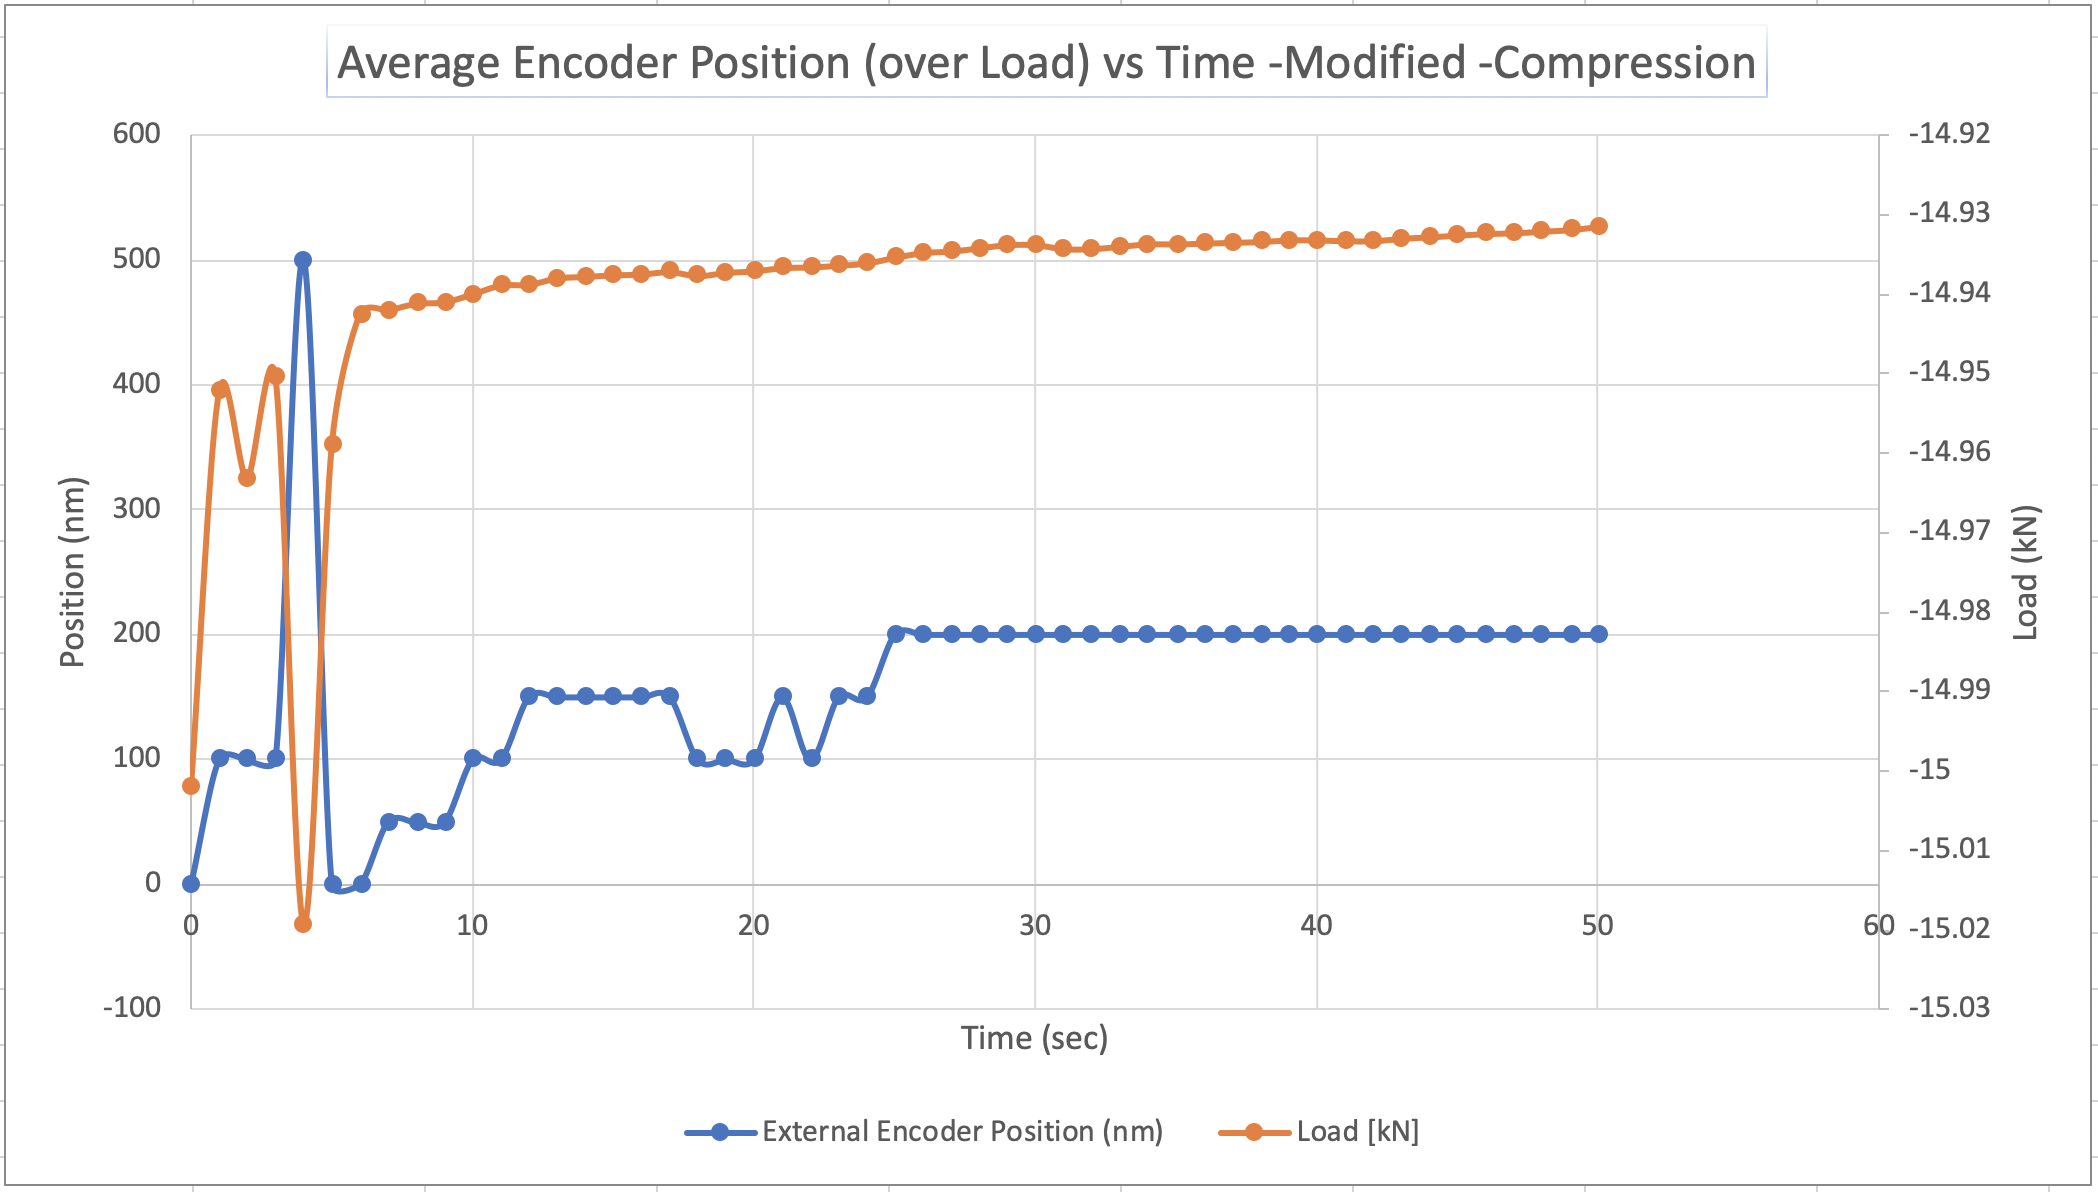
\includegraphics[width=5.98958in]{jira_imgs/4109.png}

}
\begin{tabular}{p{2cm}p{14cm}}
\toprule
Step 15 & Step Execution Status: \textbf{ Pass } \\ \hline
\end{tabular}
 Description \\
{\footnotesize
Record the actual displacement as measured by the internal encoder using
copley software.

}
\hdashrule[0.5ex]{\textwidth}{1pt}{3mm}
  Expected Result \\
{\footnotesize
Actual displacement measured by the internal encoder recorded in the
Copley Software.~

}
\hdashrule[0.5ex]{\textwidth}{1pt}{3mm}
  Actual Result \\
{\footnotesize
The Active Load Position reported by the Copley Control Software could
not be exported. However, we confirmed after every move that the
relative motion moved +/-100nm each command.

}
\begin{tabular}{p{2cm}p{14cm}}
\toprule
Step 16 & Step Execution Status: \textbf{ Pass } \\ \hline
\end{tabular}
 Description \\
{\footnotesize
Remove the 15 kN compression load.

}
\hdashrule[0.5ex]{\textwidth}{1pt}{3mm}
  Test Data \\
 {\footnotesize
\textbf{Note:~}Set Channel 0 = Channel 1 = 0V.\\[2\baselineskip]

}
\hdashrule[0.5ex]{\textwidth}{1pt}{3mm}
  Expected Result \\
{\footnotesize
Load cell reader and Load graph in the LabView showing zero
load.\\[2\baselineskip]

}
\hdashrule[0.5ex]{\textwidth}{1pt}{3mm}
  Actual Result \\
{\footnotesize
The load was removed.

}
\begin{tabular}{p{2cm}p{14cm}}
\toprule
Step 17 & Step Execution Status: \textbf{ Pass } \\ \hline
\end{tabular}
 Description \\
{\footnotesize
Compare the internal linear encoder measurement with the average of the
two external linear encoder measurements.

}
\hdashrule[0.5ex]{\textwidth}{1pt}{3mm}
  Expected Result \\
{\footnotesize
Comparison of the Displacement graphs ( External vs internal) in
LabView. The magnitude should not vary by more than 50\% from the
commanded value based on an average of the two external linear encoder
measurements.\\[2\baselineskip]

}
\hdashrule[0.5ex]{\textwidth}{1pt}{3mm}
  Actual Result \\
{\footnotesize
For the modified actuator, the displacement measured by the external
encoders were tested. The average displacement of the external encoders
did not vary by more than 50nm during the majority of the sequence of
moves.\\[2\baselineskip]This can be seen in column L of the Compression
sheet in the \emph{Resolution Test Results - Modified
Actuator.xlsx~}excel document. At the time of the greatest deviations,
there were some noise on the load cell that could have been impacting
the results. However, similar to Moog's test report, we couldn't apply
load compensation (as the step sizes are too small) to reduce the noise.
This step was still considered to be passed.

}
\begin{tabular}{p{2cm}p{14cm}}
\toprule
Step 18 & Step Execution Status: \textbf{ Pass } \\ \hline
\end{tabular}
 Description \\
{\footnotesize
With Zero load applied to the actuator, execute the following commands
to the actuator in relative positioning mode using the copley software
and the control box: extend 100nm, extend 100nm, extend 100nm, retract
100nm, extend 100nm, retract 100nm, retract 100nm, retract 100nm.

}
\hdashrule[0.5ex]{\textwidth}{1pt}{3mm}
  Test Data \\
 {\footnotesize
\textbf{Note:~}Take note of the time at which the moves are commanded.
It will be difficult to determine when the series of commands are sent
because the moves are so small.

}
\hdashrule[0.5ex]{\textwidth}{1pt}{3mm}
  Expected Result \\
{\footnotesize
All moves should move in the commanded direction.

}
\hdashrule[0.5ex]{\textwidth}{1pt}{3mm}
  Actual Result \\
{\footnotesize
Starting at the center position,\\[2\baselineskip]Moved +100nm
(11:47:27)\\[2\baselineskip]Moved +100nm
(11:47:32)\\[2\baselineskip]Moved +100nm
(11:47:38)\\[2\baselineskip]Moved -100nm
(11:47:44)\\[2\baselineskip]Moved +100nm
(11:47:49)\\[2\baselineskip]Moved -100nm
(11:47:55)\\[2\baselineskip]Moved -100nm
(11:48:01)\\[2\baselineskip]Moved -100nm
(11:48:06)\\[2\baselineskip]These are consistent to the timestamps taken
in the Zero sheet of the attached \emph{Resolution Test Results -
Modified Actuator.xlsx~}excel document

}
\begin{tabular}{p{2cm}p{14cm}}
\toprule
Step 19 & Step Execution Status: \textbf{ Pass } \\ \hline
\end{tabular}
 Description \\
{\footnotesize
Record the actual displacement as measured by average of ~the two
external encoder as Labview graph (Displacement vs Time).

}
\hdashrule[0.5ex]{\textwidth}{1pt}{3mm}
  Expected Result \\
{\footnotesize
Actual displacement measured by the average of the two external encoders
~recorded in the LabView graph.

}
\hdashrule[0.5ex]{\textwidth}{1pt}{3mm}
  Actual Result \\
{\footnotesize
The values measuring the displacement were exported from LabView into
the Zero sheet of the \emph{Resolution Test Results - Modified
Actuator.xlsx~}excel document. The average displacement is shown in blue
in the plot below:\\
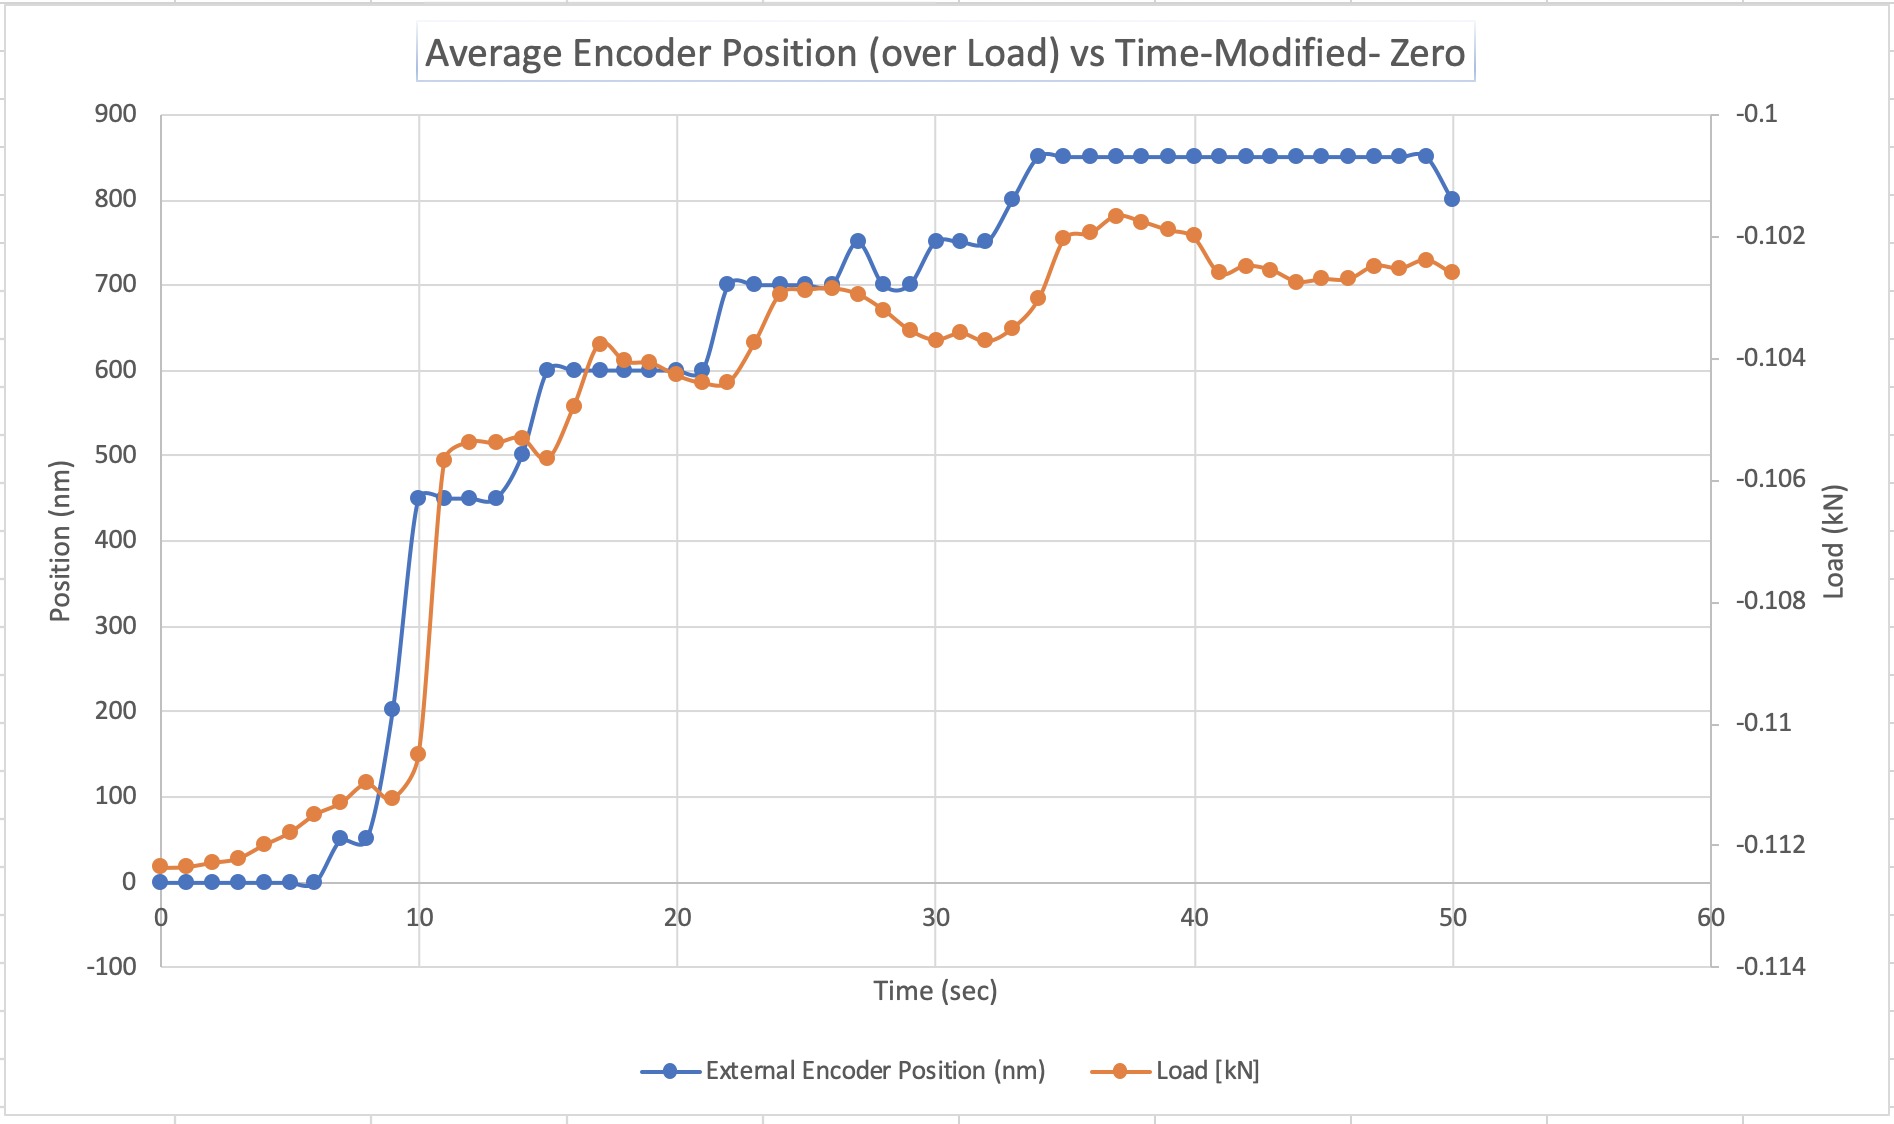
\includegraphics[width=5.98958in]{jira_imgs/4110.png}

}
\begin{tabular}{p{2cm}p{14cm}}
\toprule
Step 20 & Step Execution Status: \textbf{ Pass } \\ \hline
\end{tabular}
 Description \\
{\footnotesize
Record the actual displacement as measured by the internal encoder using
copley software.

}
\hdashrule[0.5ex]{\textwidth}{1pt}{3mm}
  Expected Result \\
{\footnotesize
Actual displacement measured by the internal encoder recorded in the
Copley Software.

}
\hdashrule[0.5ex]{\textwidth}{1pt}{3mm}
  Actual Result \\
{\footnotesize
The Active Load Position reported by the Copley Control Software could
not be exported. However, we confirmed after every move that the
relative motion moved +/-100nm each command.

}
\begin{tabular}{p{2cm}p{14cm}}
\toprule
Step 21 & Step Execution Status: \textbf{ Pass } \\ \hline
\end{tabular}
 Description \\
{\footnotesize
Compare the internal linear encoder measurement with the average of the
two external linear encoder measurements.

}
\hdashrule[0.5ex]{\textwidth}{1pt}{3mm}
  Expected Result \\
{\footnotesize
The magnitude should not vary by more than 50\% from the commanded value
based on an average of the two external linear encoder measurements.

}
\hdashrule[0.5ex]{\textwidth}{1pt}{3mm}
  Actual Result \\
{\footnotesize
The average displacement did not vary by more than 50nm during the
sequence of moves outside a few deviations.\\[2\baselineskip]This can be
seen in column L of the Zero sheet in the \emph{Resolution Test Results
- Modified Actuator.xlsx~}excel document. At the time of the greatest
deviations, there were some noise on the load cell that could have been
impacting the results. However, similar to Moog's test report, we
couldn't apply load compensation (as the step sizes are too small) to
reduce the noise. This step was still considered to be passed.

}
\begin{tabular}{p{2cm}p{14cm}}
\toprule
Step 22 & Step Execution Status: \textbf{ Pass } \\ \hline
\end{tabular}
 Description \\
{\footnotesize
Press Stop button in the VI file front panel to stop reading of the
components.

}
\hdashrule[0.5ex]{\textwidth}{1pt}{3mm}
  Expected Result \\
{\footnotesize
Graphs in the front panel of the VI file becomes static.

}
\hdashrule[0.5ex]{\textwidth}{1pt}{3mm}
  Actual Result \\
{\footnotesize
The VI's were stopped.

}
\begin{tabular}{p{2cm}p{14cm}}
\toprule
Step 23 & Step Execution Status: \textbf{ Pass } \\ \hline
\end{tabular}
 Description \\
{\footnotesize
Check if all the test results are recorded in excel spreadsheets.~

}
\hdashrule[0.5ex]{\textwidth}{1pt}{3mm}
  Expected Result \\
{\footnotesize
Test Results are recorded in the excel spreadsheets residing in the
LabView Folder directory.~

}
\hdashrule[0.5ex]{\textwidth}{1pt}{3mm}
  Actual Result \\
{\footnotesize
All test results have been recorded and collected into the
\emph{Resolution Test Results - Modified Actuator.xlsx} excel document.

}
\begin{tabular}{p{2cm}p{14cm}}
\toprule
Step 24 & Step Execution Status: \textbf{ Not Executed } \\ \hline
\end{tabular}
 Description \\
{\footnotesize
Close all the Labview VI files.

}
\hdashrule[0.5ex]{\textwidth}{1pt}{3mm}
  Test Data \\
 {\footnotesize
\textbf{Note:~}Labview can be left open in order to continue to the next
test. However, it may be necessary to reset the application before
starting the next test.

}
\hdashrule[0.5ex]{\textwidth}{1pt}{3mm}
  Expected Result \\
{\footnotesize
All the VI files are closed and Labview 2021 application window closes.~

}
\hdashrule[0.5ex]{\textwidth}{1pt}{3mm}
  Actual Result \\
{\footnotesize
The LabView VI's were stopped, but not closed.

}

\paragraph{ LVV-T2436 - Hexapod - Actuator Accuracy Test }\mbox{}\\

Version \textbf{1}.
Status \textbf{Approved}.
Open  \href{https://jira.lsstcorp.org/secure/Tests.jspa#/testCase/LVV-T2436}{\textit{ LVV-T2436 } }
test case in Jira.

To perform the actuator accuracy tests in order to verify the Hexapod
Accuracy requirements in \citeds{LTS-206}.~

\textbf{ Preconditions}:\\


Execution status: {\bf Pass }

Final comment:\\For this we started at the Zero Position:\\

\begin{itemize}
\tightlist
\item
  Copley Software: Active Load Position = \textbf{-22.008mm or -2200875
  counts}
\item
  Encoder A (D13B) = 39.4mm
\item
  Encoder B (D0BD) = 39.5mm
\end{itemize}

During this test, it can be seen in the results that there were
variations in the applied load that may have impacted the results of
this test. As a result of the noise, there were outliers to the expected
accuracy, specifically for the larger moves in mm. For the smaller moves
in um, the accuracy was less than the expected error. However, this was
expected as MOOG's original test report cites the same variation when
applying load. Therefore, load compensation was applied to the results
in an effort to reduce the noise's impact on the results. Applying load
compensation improved the overall results, but there were still some
outliers that were greater than the expected 17um for the large moves:

\begin{itemize}
\tightlist
\item
  Large scale accuracy maximum error - Tension = \textbf{22.65um}
\item
  Large scale accuracy maximum error - Compression = \textbf{24.76um}
\item
  Large scale accuracy maximum error - Zero = \textbf{41.54um}
\end{itemize}

For the smaller moves, the maximum error was less than the expected
20um:

\begin{itemize}
\tightlist
\item
  Small scale accuracy maximum error - Tension = 12.25um
\item
  Small scale accuracy maximum error - Compression = 17.7um
\item
  Small scale accuracy maximum error - Zero = 16.8um
\end{itemize}

Overall, the absolute accuracy of the actuators are not critical for the
operation of the hexapods. Therefore, the results have been recorded and
this test was marked as passed.


Detailed steps results:

\begin{tabular}{p{2cm}p{14cm}}
\toprule
Step 1 & Step Execution Status: \textbf{ Pass } \\ \hline
\end{tabular}
 Description \\
{\footnotesize
Review the Specification of the Resolute Encoder Series RL 36B ES 001 C
10 F encoder to confirm the accuracy of the encoder.

}
\hdashrule[0.5ex]{\textwidth}{1pt}{3mm}
  Expected Result \\
{\footnotesize
Accuracy should be less than 12um.

}
\hdashrule[0.5ex]{\textwidth}{1pt}{3mm}
  Actual Result \\
{\footnotesize
The same encoder was used and it was already confirmed that the accuracy
was less than 12um.~

}
\begin{tabular}{p{2cm}p{14cm}}
\toprule
Step 2 & Step Execution Status: \textbf{ Pass } \\ \hline
\end{tabular}
 Description \\
{\footnotesize
Open Labview 2021 in the computer used for Test Setup.

}
\hdashrule[0.5ex]{\textwidth}{1pt}{3mm}
  Test Data \\
 {\footnotesize
The next three steps are conditional because these steps are included as
part of the Test Setup procedure and may not be necessary if LabView is
still open.

}
\hdashrule[0.5ex]{\textwidth}{1pt}{3mm}
  Expected Result \\
{\footnotesize
Labview 2021 opens successfully.

}
\hdashrule[0.5ex]{\textwidth}{1pt}{3mm}
  Actual Result \\
{\footnotesize
Labview was opened successfully.

}
\begin{tabular}{p{2cm}p{14cm}}
\toprule
Step 3 & Step Execution Status: \textbf{ Pass } \\ \hline
\end{tabular}
 Description \\
{\footnotesize
Run the following VI's:

\begin{itemize}
\tightlist
\item
  Encoder A (D13B) and Load Cell.vi
\item
  Encoder B (D0BD).vi
\end{itemize}

}
\hdashrule[0.5ex]{\textwidth}{1pt}{3mm}
  Expected Result \\
{\footnotesize
Front panel of VI's open without any error.

}
\hdashrule[0.5ex]{\textwidth}{1pt}{3mm}
  Actual Result \\
{\footnotesize
LabView was ran without any issue.‚Äã‚Äã‚Äã‚Äã

}
\begin{tabular}{p{2cm}p{14cm}}
\toprule
Step 4 & Step Execution Status: \textbf{ Pass } \\ \hline
\end{tabular}
 Description \\
{\footnotesize
Click Run button on the on the block diagram toolbar of the Labview VI
front panel.

}
\hdashrule[0.5ex]{\textwidth}{1pt}{3mm}
  Expected Result \\
{\footnotesize
LabView VI and associated sub Vi runs successfully. The graphs should
start to be populated with data once the run button is pressed.

}
\hdashrule[0.5ex]{\textwidth}{1pt}{3mm}
  Actual Result \\
{\footnotesize
LabView was ran without any issue.

}
\begin{tabular}{p{2cm}p{14cm}}
\toprule
Step 5 & Step Execution Status: \textbf{ Pass } \\ \hline
\end{tabular}
 Description \\
{\footnotesize
Position the actuator at its center of stroke position using the control
box and copley software.\\[2\baselineskip]

}
\hdashrule[0.5ex]{\textwidth}{1pt}{3mm}
  Test Data \\
 {\footnotesize
\textbf{Note:~}The original zero position/center of stroke position was
determined to be a linear encoder reading of 40mm. For the purpose of
this test, the same center of stroke position will be used.

}
\hdashrule[0.5ex]{\textwidth}{1pt}{3mm}
  Expected Result \\
{\footnotesize
Actuator positioned at its center of stroke position ~confirmed by
encoder reading in the LabView.\\[2\baselineskip]

}
\hdashrule[0.5ex]{\textwidth}{1pt}{3mm}
  Actual Result \\
{\footnotesize
After the actuator was modified, the center of stroke position (or zero
position) was seen to be -20.008mm. The actuator was placed at this zero
position.

}
\begin{tabular}{p{2cm}p{14cm}}
\toprule
Step 6 & Step Execution Status: \textbf{ Pass } \\ \hline
\end{tabular}
 Description \\
{\footnotesize
Apply a force of +15kN.

}
\hdashrule[0.5ex]{\textwidth}{1pt}{3mm}
  Test Data \\
 {\footnotesize
\textbf{Note:~}In order to apply a tension force of +15 kN, set Channel
1 = 2.19V and Channel 0 = 0V.

}
\hdashrule[0.5ex]{\textwidth}{1pt}{3mm}
  Expected Result \\
{\footnotesize
Load cell reader shows the applied +15 kN \textbf{tension} force.\\
LabView displays the voltage being applied.

}
\hdashrule[0.5ex]{\textwidth}{1pt}{3mm}
  Actual Result \\
{\footnotesize
+15kN load was applied.

}
\begin{tabular}{p{2cm}p{14cm}}
\toprule
Step 7 & Step Execution Status: \textbf{ Pass } \\ \hline
\end{tabular}
 Description \\
{\footnotesize
Record the load cell value in the LabView in the form of Load vs Time
graph.

}
\hdashrule[0.5ex]{\textwidth}{1pt}{3mm}
  Expected Result \\
{\footnotesize
LabView load graph (Load vs Time) shows +15 kN tension force applied.

}
\hdashrule[0.5ex]{\textwidth}{1pt}{3mm}
  Actual Result \\
{\footnotesize
The load was recorded into a Load vs Time graph in Labview and the data
was exported into excel. The raw results can be found in the
\emph{Accuracy\_Test\_Raw\_Data\_Modified\_Actuator.zip}.~

}
\begin{tabular}{p{2cm}p{14cm}}
\toprule
Step 8 & Step Execution Status: \textbf{ Pass } \\ \hline
\end{tabular}
 Description \\
{\footnotesize
Command the following moves to the actuator using the copley software
and the control box in absolute mode: +3.5mm, +7mm, +10.5mm, +14mm,
-3.5mm, -7mm, -10.5mm, -14mm.\\[2\baselineskip]

}
\hdashrule[0.5ex]{\textwidth}{1pt}{3mm}
  Expected Result \\
{\footnotesize
All moves should move in the commanded direction.

}
\hdashrule[0.5ex]{\textwidth}{1pt}{3mm}
  Actual Result \\
{\footnotesize
+3.5mm = 3500000 counts\\
Active Load Position = 3.50mm\\[2\baselineskip]+7mm = 7000000 counts\\
Active Load Position = 7.00mm\\[2\baselineskip]+10.5mm = 10500000
counts\\
Active Load Position = 10.50mm\\[2\baselineskip]+14mm = 14000000
counts\\
Active Load Position = 13.99mm\\[2\baselineskip]-3.5mm = 3500000
counts\\
Active Load Position = -3.49mm\\[2\baselineskip]-7mm = 7000000 counts\\
Active Load Position = -6.99mm\\[2\baselineskip]-10.5mm = 10500000
counts\\
Active Load Position = 10.50mm\\[2\baselineskip]-14mm = 14000000
counts\\
Active Load Position = -14.00mm

}
\begin{tabular}{p{2cm}p{14cm}}
\toprule
Step 9 & Step Execution Status: \textbf{ Pass } \\ \hline
\end{tabular}
 Description \\
{\footnotesize
Record the actual displacement as measured by the two external encoders
as LabView graph (Displacement vs Time).

}
\hdashrule[0.5ex]{\textwidth}{1pt}{3mm}
  Expected Result \\
{\footnotesize
Actual displacement measured by the average of the two external encoders
~recorded in the LabView graph.

}
\hdashrule[0.5ex]{\textwidth}{1pt}{3mm}
  Actual Result \\
{\footnotesize
The recorded data was exported from LabView into the Accuracy-Large
Scale sheet of the
\href{https://docushare.lsst.org/docushare/dsweb/Services/Document-55067}{\emph{Accuracy
Test Results -Modified vs Unmodified.xlsx}} excel document. The plotted
values can be seen below, where the blue and orange line represents the
average displacement of the external encoders and the grey line
represents the commanded position:\\
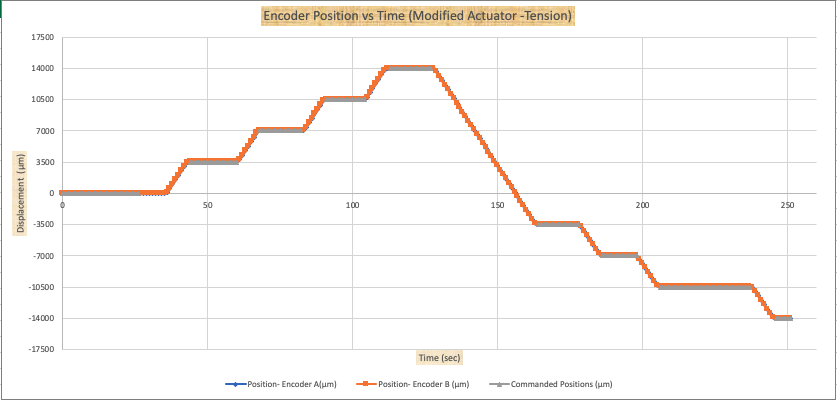
\includegraphics[width=5.98958in]{jira_imgs/4120.png}

}
\begin{tabular}{p{2cm}p{14cm}}
\toprule
Step 10 & Step Execution Status: \textbf{ Pass } \\ \hline
\end{tabular}
 Description \\
{\footnotesize
Record the actual displacement as measured by the internal encoder using
copley software.

}
\hdashrule[0.5ex]{\textwidth}{1pt}{3mm}
  Expected Result \\
{\footnotesize
Actual displacement measured by the internal encoder recorded in the
Copley Software.

}
\hdashrule[0.5ex]{\textwidth}{1pt}{3mm}
  Actual Result \\
{\footnotesize
The Active Load Position reported by the Copley Control Software could
not be exported. However, we confirmed the absolute position movements
as reported by the Copley Control Software.

}
\begin{tabular}{p{2cm}p{14cm}}
\toprule
Step 11 & Step Execution Status: \textbf{ Pass } \\ \hline
\end{tabular}
 Description \\
{\footnotesize
Ensure that the load cell signal did not vary significantly during the
test which would introduce compliance errors.

}
\hdashrule[0.5ex]{\textwidth}{1pt}{3mm}
  Expected Result \\
{\footnotesize
The tension load should remain close to +15kN throughout the
displacement movements and display in the Load vs Time graph in LabView.

}
\hdashrule[0.5ex]{\textwidth}{1pt}{3mm}
  Actual Result \\
{\footnotesize
There were some variations to the load while the actuator was moved.
Therefore, load compensation was applied similar to MOOG's procedure. As
a result, the average accuracy error can be seen below in orange:\\
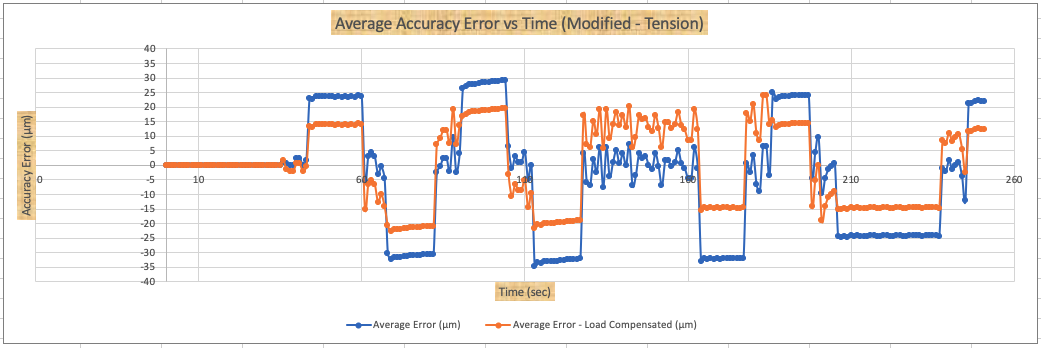
\includegraphics[width=5.98958in]{jira_imgs/4119.png}With the load
compensation, the average accuracy error was significantly reduced, but
still above the expected 20um at times. This plot can be found on
the~Accuracy- Large Scale~sheet of the\emph{~Accuracy Test Results
-Modified vs Unmodifed.xlsx} document.

}
\begin{tabular}{p{2cm}p{14cm}}
\toprule
Step 12 & Step Execution Status: \textbf{ Pass } \\ \hline
\end{tabular}
 Description \\
{\footnotesize
Compare the internal linear encoder measurement with the average of the
two external linear encoder measurements in LabView.

}
\hdashrule[0.5ex]{\textwidth}{1pt}{3mm}
  Expected Result \\
{\footnotesize
\textbf{The large-scale accuracy error \textless{}= 17um.}

}
\hdashrule[0.5ex]{\textwidth}{1pt}{3mm}
  Actual Result \\
{\footnotesize
As seen in the Average Accuracy Error vs. Time (Modified - Tension) plot
in the previous step, even with load compensation we couldn't reduce the
noise applied to the encoders and actuator. However, these types of
deviations were seen in MOOG's original test report. Additionally, since
the accuracy of the actuator isn't so critical to the overall accuracy
of the hexapod, this step was marked as passed.

}
\begin{tabular}{p{2cm}p{14cm}}
\toprule
Step 13 & Step Execution Status: \textbf{ Pass } \\ \hline
\end{tabular}
 Description \\
{\footnotesize
Restart at the zero position.

}
\hdashrule[0.5ex]{\textwidth}{1pt}{3mm}
  Test Data \\
 {\footnotesize
\textbf{Note:~}Command the actuator to the absolute zero position.

}
\hdashrule[0.5ex]{\textwidth}{1pt}{3mm}
  Expected Result \\
{\footnotesize
Actuator positioned at its center of stroke position ~confirmed by
encoder reading in the LabView.

}
\hdashrule[0.5ex]{\textwidth}{1pt}{3mm}
  Actual Result \\
{\footnotesize
The actuator was commanded back to the zero position.

}
\begin{tabular}{p{2cm}p{14cm}}
\toprule
Step 14 & Step Execution Status: \textbf{ Pass } \\ \hline
\end{tabular}
 Description \\
{\footnotesize
With a +15kN tension load applied to the actuator, command the following
moves the copley software and the control box in absolute mode: +100um,
+200um, +300um, +400um, -100um, -200um, -300um, -400um.

}
\hdashrule[0.5ex]{\textwidth}{1pt}{3mm}
  Expected Result \\
{\footnotesize
All moves should move in the commanded direction.

}
\hdashrule[0.5ex]{\textwidth}{1pt}{3mm}
  Actual Result \\
{\footnotesize
+100um = 100000 counts\\
Active Load Position = 0.1000mm\\[2\baselineskip]+200um = 200000
counts\\
Active Load Position = 0.2000mm\\[2\baselineskip]+300um = 300000
counts\\
Active Load Position = 0.3000mm\\[2\baselineskip]+400um = 400000
counts\\
Active Load Position = 0.4001mm\\[2\baselineskip]-100um = -100000
counts\\
Active Load Position = -0.0999mm\\[2\baselineskip]-200um = -200000
counts\\
Active Load Position = -0.2008mm\\[2\baselineskip]-300um =-300000
counts\\
Active Load Position = -0.3034mm\\[2\baselineskip]-400um = -400000
counts\\
Active Load Position = -0.3999mm

}
\begin{tabular}{p{2cm}p{14cm}}
\toprule
Step 15 & Step Execution Status: \textbf{ Pass } \\ \hline
\end{tabular}
 Description \\
{\footnotesize
Record the actual displacement as measured by the two external encoders
as LabView graph (Displacement vs Time).

}
\hdashrule[0.5ex]{\textwidth}{1pt}{3mm}
  Expected Result \\
{\footnotesize
Actual displacement measured by the average of the two external encoders
~recorded in the LabView graph.

}
\hdashrule[0.5ex]{\textwidth}{1pt}{3mm}
  Actual Result \\
{\footnotesize
The recorded data was exported from LabView into the~Accuracy-Small
Scale sheet of the ~\emph{Accuracy Test Results -Modified vs
Unmodified.xlsx~}excel document. The plotted values can be seen below
where the blue line represents the average displacement of the external
encoders and the orange line represents the commanded position:\\
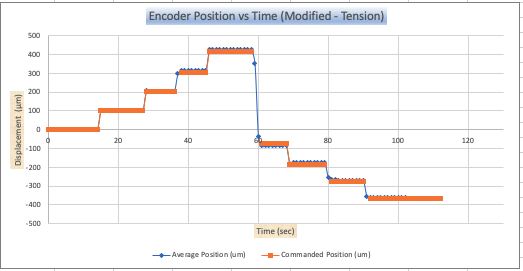
\includegraphics[width=5.98958in]{jira_imgs/4118.png}

}
\begin{tabular}{p{2cm}p{14cm}}
\toprule
Step 16 & Step Execution Status: \textbf{ Pass } \\ \hline
\end{tabular}
 Description \\
{\footnotesize
Record the actual displacement as measured by the internal encoder using
copley software.

}
\hdashrule[0.5ex]{\textwidth}{1pt}{3mm}
  Expected Result \\
{\footnotesize
Actual displacement measured by the internal encoder recorded in the
Copley Software.

}
\hdashrule[0.5ex]{\textwidth}{1pt}{3mm}
  Actual Result \\
{\footnotesize
The Active Load Position reported by the Copley Control Software could
not be exported. However, we monitored the absolute position movements
at the time of the test as reported by the Copley Control Software.

}
\begin{tabular}{p{2cm}p{14cm}}
\toprule
Step 17 & Step Execution Status: \textbf{ Pass } \\ \hline
\end{tabular}
 Description \\
{\footnotesize
Ensure that the load cell signal did not vary significantly during the
test which would introduce compliance errors.

}
\hdashrule[0.5ex]{\textwidth}{1pt}{3mm}
  Expected Result \\
{\footnotesize
The tension load should remain close to 15kN throughout the test and
display in the Load vs Time graph in LabView.

}
\hdashrule[0.5ex]{\textwidth}{1pt}{3mm}
  Actual Result \\
{\footnotesize
As seen in the plot attached to Step 15, the variation in load did not
have any significant impact to the actuator's ability to comply to the
commanded position. As a result, the average accuracy error can be seen
below in blue:\\
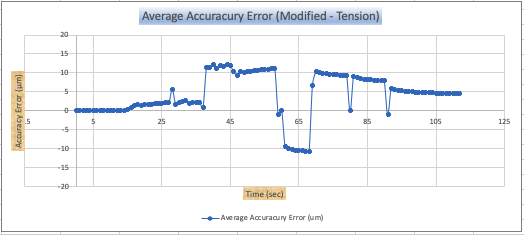
\includegraphics[width=5.98958in]{jira_imgs/4117.png}\\[2\baselineskip]This
plot can be found on the~Accuracy- Small Scale~sheet of
the\emph{~Accuracy Test Results -Modified vs Unmodifed.xlsx} document.

}
\begin{tabular}{p{2cm}p{14cm}}
\toprule
Step 18 & Step Execution Status: \textbf{ Pass } \\ \hline
\end{tabular}
 Description \\
{\footnotesize
Compare the internal linear encoder measurement with the average of the
two external linear encoder measurements.

}
\hdashrule[0.5ex]{\textwidth}{1pt}{3mm}
  Expected Result \\
{\footnotesize
\textbf{The small-scale accuracy error \textless{}= 20um.}

}
\hdashrule[0.5ex]{\textwidth}{1pt}{3mm}
  Actual Result \\
{\footnotesize
By analyzing the data from the external linear encoder measurements, the
small-scale accuracy error was seen to be within \textless{}= 20um with
load compensation. This can be seen in the Average Accuracy Error -
Modified - Tension plot in the previous step.

}
\begin{tabular}{p{2cm}p{14cm}}
\toprule
Step 19 & Step Execution Status: \textbf{ Pass } \\ \hline
\end{tabular}
 Description \\
{\footnotesize
Remove the 15 kN tension load.

}
\hdashrule[0.5ex]{\textwidth}{1pt}{3mm}
  Test Data \\
 {\footnotesize
\textbf{Note:~}Set Channel 0 = Channel 1 = 0V.

}
\hdashrule[0.5ex]{\textwidth}{1pt}{3mm}
  Expected Result \\
{\footnotesize
Load cell reader and Load graph in the LabView showing zero load.

}
\hdashrule[0.5ex]{\textwidth}{1pt}{3mm}
  Actual Result \\
{\footnotesize
The tension force was removed

}
\begin{tabular}{p{2cm}p{14cm}}
\toprule
Step 20 & Step Execution Status: \textbf{ Pass } \\ \hline
\end{tabular}
 Description \\
{\footnotesize
Restart at the zero position.

}
\hdashrule[0.5ex]{\textwidth}{1pt}{3mm}
  Test Data \\
 {\footnotesize
\textbf{Note:~}Command the actuator to the absolute zero position.

}
\hdashrule[0.5ex]{\textwidth}{1pt}{3mm}
  Expected Result \\
{\footnotesize
Actuator positioned at its center of stroke position ~confirmed by
encoder reading in the LabView.

}
\hdashrule[0.5ex]{\textwidth}{1pt}{3mm}
  Actual Result \\
{\footnotesize
The actuator was commanded back to the absolute zero position.

}
\begin{tabular}{p{2cm}p{14cm}}
\toprule
Step 21 & Step Execution Status: \textbf{ Pass } \\ \hline
\end{tabular}
 Description \\
{\footnotesize
Apply a -15kN force.

}
\hdashrule[0.5ex]{\textwidth}{1pt}{3mm}
  Test Data \\
 {\footnotesize
\textbf{Note:~}In order to apply a compression force of -15 kN, set
Channel 0 = 2.19V and Channel 1 = 0V.

}
\hdashrule[0.5ex]{\textwidth}{1pt}{3mm}
  Expected Result \\
{\footnotesize
Load cell reader shows the applied -15kN \textbf{compression} force.\\
LabView displays the voltage being applied.

}
\hdashrule[0.5ex]{\textwidth}{1pt}{3mm}
  Actual Result \\
{\footnotesize
The Compression valve was set to 2.19V to apply the load in compression.

}
\begin{tabular}{p{2cm}p{14cm}}
\toprule
Step 22 & Step Execution Status: \textbf{ Pass } \\ \hline
\end{tabular}
 Description \\
{\footnotesize
Command the following moves using the copley software and the control
box in absolute mode: +3.5mm, +7mm, +10.5mm, +14mm, -3.5mm, -7mm,
-10.5mm, -14mm.\\[2\baselineskip]

}
\hdashrule[0.5ex]{\textwidth}{1pt}{3mm}
  Expected Result \\
{\footnotesize
All moves should move in the commanded direction.

}
\hdashrule[0.5ex]{\textwidth}{1pt}{3mm}
  Actual Result \\
{\footnotesize
+3.5mm = 3500000 counts\\
Active Load Position = 3.50mm\\[2\baselineskip]+7mm = 7000000 counts\\
Active Load Position = 7.00mm\\[2\baselineskip]+10.5mm = 10500000
counts\\
Active Load Position = 10.50mm\\[2\baselineskip]+14mm = 14000000
counts\\
Active Load Position = 13.99mm\\[2\baselineskip]-3.5mm = 3500000
counts\\
Active Load Position = -3.49mm\\[2\baselineskip]-7mm = 7000000 counts\\
Active Load Position = -6.99mm\\[2\baselineskip]-10.5mm = 10500000
counts\\
Active Load Position = 10.50mm\\[2\baselineskip]-14mm = 14000000
counts\\
Active Load Position = -14.00mm

}
\begin{tabular}{p{2cm}p{14cm}}
\toprule
Step 23 & Step Execution Status: \textbf{ Pass } \\ \hline
\end{tabular}
 Description \\
{\footnotesize
Record the actual displacement as measured by average of ~the two
external encoder as Labview graph (Displacement vs Time).

}
\hdashrule[0.5ex]{\textwidth}{1pt}{3mm}
  Expected Result \\
{\footnotesize
Actual displacement measured by the average of the two external encoders
~recorded in the LabView graph.

}
\hdashrule[0.5ex]{\textwidth}{1pt}{3mm}
  Actual Result \\
{\footnotesize
The recorded data was exported from LabView into the Accuracy-Large
Scale sheet of the \emph{~Accuracy Test Results -Modified vs
Unmodified.xlsx~}excel document. The plotted values can be seen below
where the blue and orange line represents the average displacement of
the external encoders and the grey line represents the commanded
position:\\
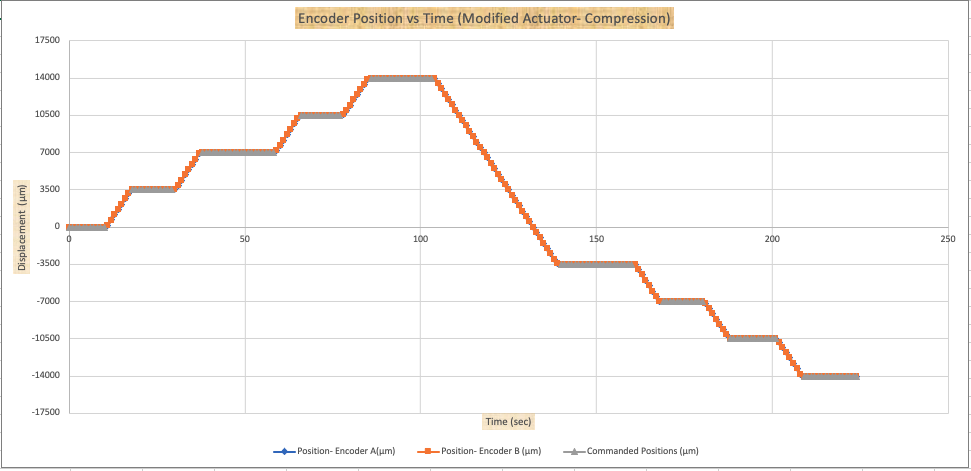
\includegraphics[width=5.98958in]{jira_imgs/4121.png}

}
\begin{tabular}{p{2cm}p{14cm}}
\toprule
Step 24 & Step Execution Status: \textbf{ Pass } \\ \hline
\end{tabular}
 Description \\
{\footnotesize
Record the actual displacement as measured by the internal encoder using
copley software.

}
\hdashrule[0.5ex]{\textwidth}{1pt}{3mm}
  Expected Result \\
{\footnotesize
Actual displacement measured by the internal encoder recorded in the
Copley Software.

}
\hdashrule[0.5ex]{\textwidth}{1pt}{3mm}
  Actual Result \\
{\footnotesize
The Active Load Position reported by the Copley Control Software could
not be exported. However, we confirmed the absolute position movements
as reported by the Copley Control Software.

}
\begin{tabular}{p{2cm}p{14cm}}
\toprule
Step 25 & Step Execution Status: \textbf{ Pass } \\ \hline
\end{tabular}
 Description \\
{\footnotesize
Ensure that the load cell signal did not vary significantly during the
test which would introduce compliance errors.

}
\hdashrule[0.5ex]{\textwidth}{1pt}{3mm}
  Expected Result \\
{\footnotesize
The compression load should remain close to 15kN throughout the test and
display in the Load vs Time graph in LabView.

}
\hdashrule[0.5ex]{\textwidth}{1pt}{3mm}
  Actual Result \\
{\footnotesize
There were some variations to the load while the actuator was moved.
Therefore, load compensation was applied similar to MOOG's procedure. As
a result, the average accuracy error can be seen below in orange:\\
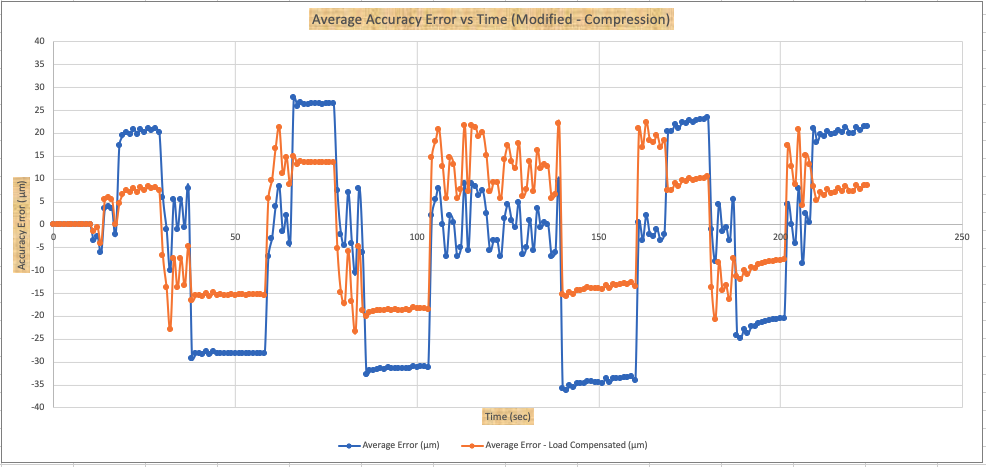
\includegraphics[width=5.98958in]{jira_imgs/4122.png}With the load
compensation, the average accuracy error was significantly reduced. This
Average Accuracy vs Time (Modified - Compression) plot can be found on
the~Accuracy- Large Scale~sheet of the\emph{~Accuracy Test Results
-Modified vs Unmodifed.xlsx} document.

}
\begin{tabular}{p{2cm}p{14cm}}
\toprule
Step 26 & Step Execution Status: \textbf{ Pass } \\ \hline
\end{tabular}
 Description \\
{\footnotesize
Compare the internal linear encoder measurement with the average of the
two external linear encoder measurements.

}
\hdashrule[0.5ex]{\textwidth}{1pt}{3mm}
  Expected Result \\
{\footnotesize
\textbf{The large-scale accuracy error \textless{}= 17um.}

}
\hdashrule[0.5ex]{\textwidth}{1pt}{3mm}
  Actual Result \\
{\footnotesize
By analyzing the data from the external linear encoder measurements, the
large-scale accuracy error was seen to be mostly within \textless{}=
17um with load compensation. This can be seen in the Average Accuracy
Error vs. Time (Modified - Compression) plot in the previous step. There
were some outliers noted, but this was expected as MOOG's original
report showed noise on the load cell and the external encoders. Although
load compensation was applied, there were still some errors that can be
attributed to the noise. Since this does not impact our ability to meet
the hexapod level requirement, this was marked as passed.

}
\begin{tabular}{p{2cm}p{14cm}}
\toprule
Step 27 & Step Execution Status: \textbf{ Pass } \\ \hline
\end{tabular}
 Description \\
{\footnotesize
Restart at the zero position.

}
\hdashrule[0.5ex]{\textwidth}{1pt}{3mm}
  Test Data \\
 {\footnotesize
\textbf{Note:~}The original zero position/center of stroke position was
determined to be a linear encoder reading of 40mm. For the purpose of
this test, the same center of stroke position will be used.

}
\hdashrule[0.5ex]{\textwidth}{1pt}{3mm}
  Expected Result \\
{\footnotesize
Actuator positioned at its center of stroke position ~confirmed by
encoder reading in the LabView.

}
\hdashrule[0.5ex]{\textwidth}{1pt}{3mm}
  Actual Result \\
{\footnotesize
The actuator was commanded back to the absolute zero position.

}
\begin{tabular}{p{2cm}p{14cm}}
\toprule
Step 28 & Step Execution Status: \textbf{ Pass } \\ \hline
\end{tabular}
 Description \\
{\footnotesize
With a 15 kN compression load applied to the actuator, command the
following moves using the copley software and the control box in
absolute mode: +100um, +200um, +300um, +400um, -100um, -200um, -300um,
-400um.

}
\hdashrule[0.5ex]{\textwidth}{1pt}{3mm}
  Expected Result \\
{\footnotesize
All moves should move in the commanded direction.

}
\hdashrule[0.5ex]{\textwidth}{1pt}{3mm}
  Actual Result \\
{\footnotesize
+100um = 100000 counts\\
Active Load Position = 0.1000mm\\[2\baselineskip]+200um = 200000
counts\\
Active Load Position = 0.1999mm\\[2\baselineskip]+300um = 300000
counts\\
Active Load Position = 0.3000mm\\[2\baselineskip]+400um = 400000
counts\\
Active Load Position = 0.4001mm\\[2\baselineskip]-100um = -100000
counts\\
Active Load Position = -0.0999mm\\[2\baselineskip]-200um = -200000
counts\\
Active Load Position = -0.1998mm\\[2\baselineskip]-300um =-300000
counts\\
Active Load Position = -0.2997mm\\[2\baselineskip]-400um = -400000
counts\\
Active Load Position = -0.3999mm

}
\begin{tabular}{p{2cm}p{14cm}}
\toprule
Step 29 & Step Execution Status: \textbf{ Pass } \\ \hline
\end{tabular}
 Description \\
{\footnotesize
Record the actual displacement as measured by average of ~the two
external encoder as Labview graph (Displacement vs. Time).

}
\hdashrule[0.5ex]{\textwidth}{1pt}{3mm}
  Expected Result \\
{\footnotesize
Actual displacement measured by the average of the two external encoders
~recorded in the LabView graph.

}
\hdashrule[0.5ex]{\textwidth}{1pt}{3mm}
  Actual Result \\
{\footnotesize
The recorded data was exported from LabView into the~Accuracy-Small
Scale sheet of the~\emph{Accuracy Test Results -Modified vs
Unmodified.xlsx} excel document. The plotted values can be seen below
where the blue line represents the average displacement of the external
encoders and the orange line represents the commanded position:\\
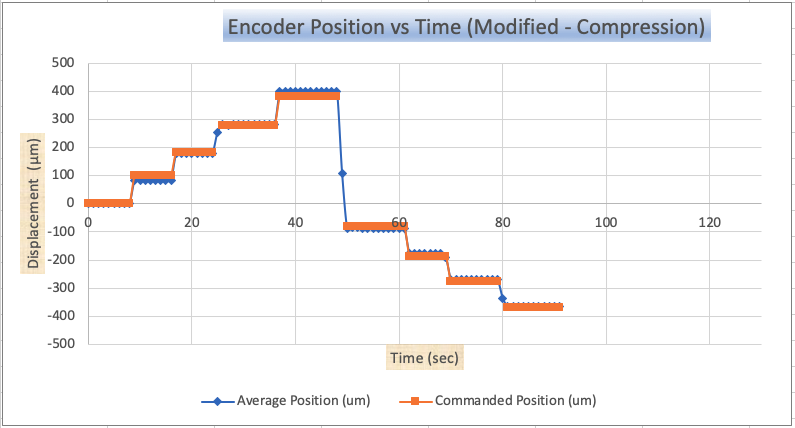
\includegraphics[width=5.98958in]{jira_imgs/4116.png}

}
\begin{tabular}{p{2cm}p{14cm}}
\toprule
Step 30 & Step Execution Status: \textbf{ Pass } \\ \hline
\end{tabular}
 Description \\
{\footnotesize
Record the actual displacement as measured by the internal encoder using
copley software.

}
\hdashrule[0.5ex]{\textwidth}{1pt}{3mm}
  Expected Result \\
{\footnotesize
Actual displacement measured by the internal encoder recorded in the
Copley Software.

}
\hdashrule[0.5ex]{\textwidth}{1pt}{3mm}
  Actual Result \\
{\footnotesize
The Active Load Position reported by the Copley Control Software could
not be exported. However, we monitored the absolute position movements
at the time of the test as reported by the Copley Control Software.

}
\begin{tabular}{p{2cm}p{14cm}}
\toprule
Step 31 & Step Execution Status: \textbf{ Pass } \\ \hline
\end{tabular}
 Description \\
{\footnotesize
Ensure that the load cell signal did not vary significantly during the
test which would introduce compliance errors.

}
\hdashrule[0.5ex]{\textwidth}{1pt}{3mm}
  Expected Result \\
{\footnotesize
The compression load should remain close to 15kN throughout the test and
displays in the Load vs Time graph in the LabView.

}
\hdashrule[0.5ex]{\textwidth}{1pt}{3mm}
  Actual Result \\
{\footnotesize
As seen in the plot attached to Step 29, the variation in load did not
have any significant impact to the actuator's ability to comply to the
commanded position. As a result, the average accuracy error can be seen
below in blue:\\
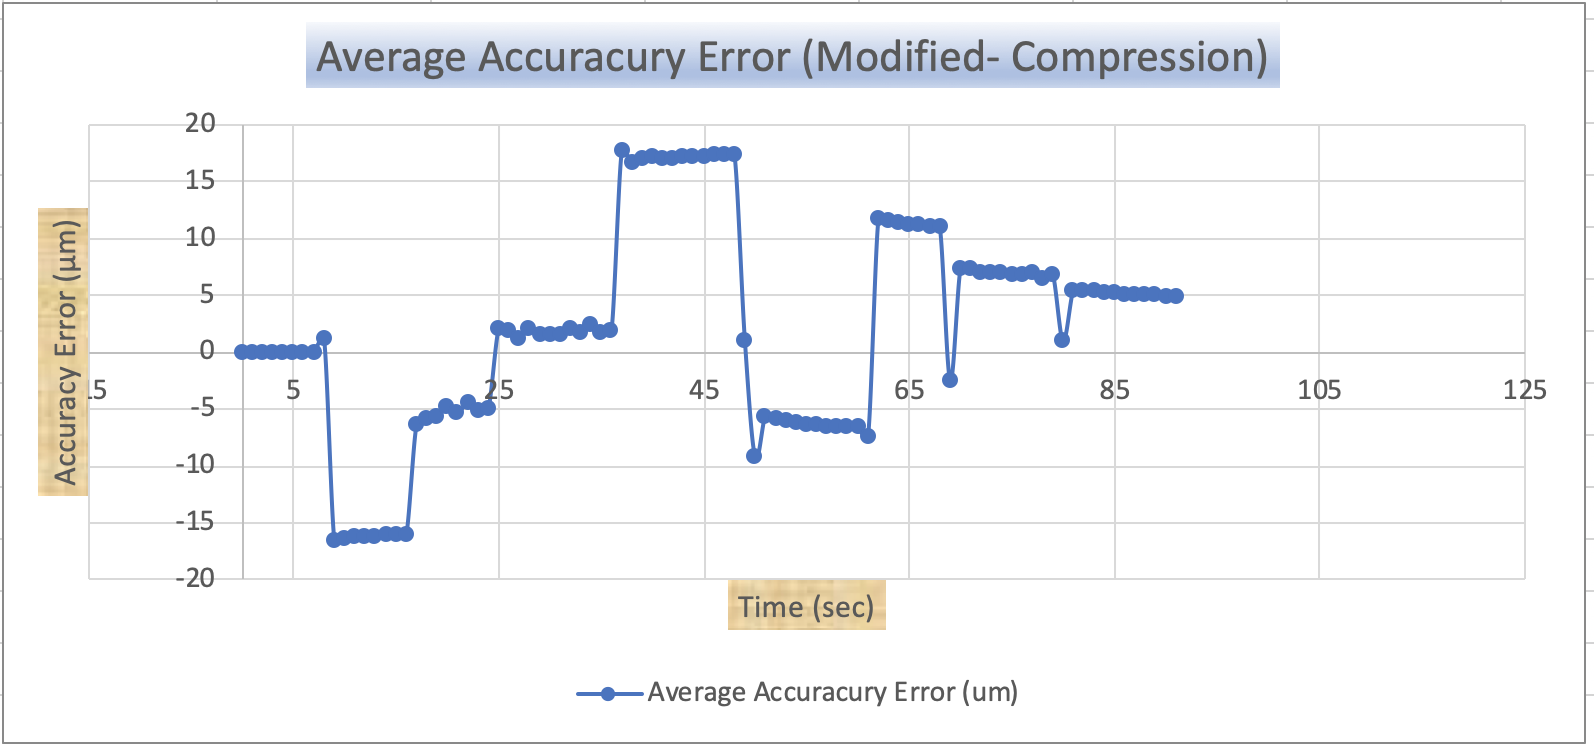
\includegraphics[width=5.98958in]{jira_imgs/4115.png}

}
\begin{tabular}{p{2cm}p{14cm}}
\toprule
Step 32 & Step Execution Status: \textbf{ Pass } \\ \hline
\end{tabular}
 Description \\
{\footnotesize
Compare the internal linear encoder measurement with the average of the
two external linear encoder measurements.

}
\hdashrule[0.5ex]{\textwidth}{1pt}{3mm}
  Expected Result \\
{\footnotesize
\textbf{The small-scale accuracy error \textless{}= 20um.}

}
\hdashrule[0.5ex]{\textwidth}{1pt}{3mm}
  Actual Result \\
{\footnotesize
By analyzing the data from the external linear encoder measurements, the
small-scale accuracy error was seen to be within \textless{}= 20um with
load compensation. This can be seen in the Average Accuracy Error
(Modified - Compression) plot in the previous step.

}
\begin{tabular}{p{2cm}p{14cm}}
\toprule
Step 33 & Step Execution Status: \textbf{ Pass } \\ \hline
\end{tabular}
 Description \\
{\footnotesize
Remove the 15 kN compression load.

}
\hdashrule[0.5ex]{\textwidth}{1pt}{3mm}
  Test Data \\
 {\footnotesize
\textbf{Note:~}Set Channel 0 = Channel 1 = 0V.

}
\hdashrule[0.5ex]{\textwidth}{1pt}{3mm}
  Expected Result \\
{\footnotesize
Load cell reader and Load graph in the LabView showing zero
load.\\[2\baselineskip]

}
\hdashrule[0.5ex]{\textwidth}{1pt}{3mm}
  Actual Result \\
{\footnotesize
Compression load was removed.

}
\begin{tabular}{p{2cm}p{14cm}}
\toprule
Step 34 & Step Execution Status: \textbf{ Pass } \\ \hline
\end{tabular}
 Description \\
{\footnotesize
Restart at the zero position.

}
\hdashrule[0.5ex]{\textwidth}{1pt}{3mm}
  Test Data \\
 {\footnotesize
\textbf{Note:~}Command the actuator to the absolute zero position.

}
\hdashrule[0.5ex]{\textwidth}{1pt}{3mm}
  Expected Result \\
{\footnotesize
Actuator positioned at its center of stroke position ~confirmed by
encoder reading in the LabView.

}
\hdashrule[0.5ex]{\textwidth}{1pt}{3mm}
  Actual Result \\
{\footnotesize
The actuator was commanded back to the absolute zero position.

}
\begin{tabular}{p{2cm}p{14cm}}
\toprule
Step 35 & Step Execution Status: \textbf{ Pass } \\ \hline
\end{tabular}
 Description \\
{\footnotesize
With ``zero'' load applied to the actuator, command the following moves
using the copley software and the control box in absolute mode: +3.5mm,
+7mm, +10.5mm, +14mm, -3.5mm, -7mm, -10.5mm, -14mm.

}
\hdashrule[0.5ex]{\textwidth}{1pt}{3mm}
  Expected Result \\
{\footnotesize
All moves should move in the commanded direction.

}
\hdashrule[0.5ex]{\textwidth}{1pt}{3mm}
  Actual Result \\
{\footnotesize
+3.5mm = 3500000 counts\\
Active Load Position = 3.50mm\\[2\baselineskip]+7mm = 7000000 counts\\
Active Load Position = 7.00mm\\[2\baselineskip]+10.5mm = 10500000
counts\\
Active Load Position = 10.50mm\\[2\baselineskip]+14mm = 14000000
counts\\
Active Load Position = 14.00mm\\[2\baselineskip]-3.5mm = 3500000
counts\\
Active Load Position = -3.49mm\\[2\baselineskip]-7mm = 7000000 counts\\
Active Load Position = -6.99mm\\[2\baselineskip]-10.5mm = 10500000
counts\\
Active Load Position = -10.49mm\\[2\baselineskip]-14mm = 14000000
counts\\
Active Load Position = -13.99mm

}
\begin{tabular}{p{2cm}p{14cm}}
\toprule
Step 36 & Step Execution Status: \textbf{ Pass } \\ \hline
\end{tabular}
 Description \\
{\footnotesize
Record the actual displacement as measured by average of ~the two
external encoder as Labview graph (Displacement vs Time).

}
\hdashrule[0.5ex]{\textwidth}{1pt}{3mm}
  Expected Result \\
{\footnotesize
Actual displacement measured by the average of the two external encoders
~recorded in the LabView graph.

}
\hdashrule[0.5ex]{\textwidth}{1pt}{3mm}
  Actual Result \\
{\footnotesize
The recorded data was exported from LabView into the Accuracy-Large
Scale sheet of the \emph{Accuracy Test Results -Modified vs
Unmodified.xlsx} excel document. The plotted values can be seen below,
where the blue and orange line represents the average displacement of
the external encoders and the grey line represents the commanded
position:\\
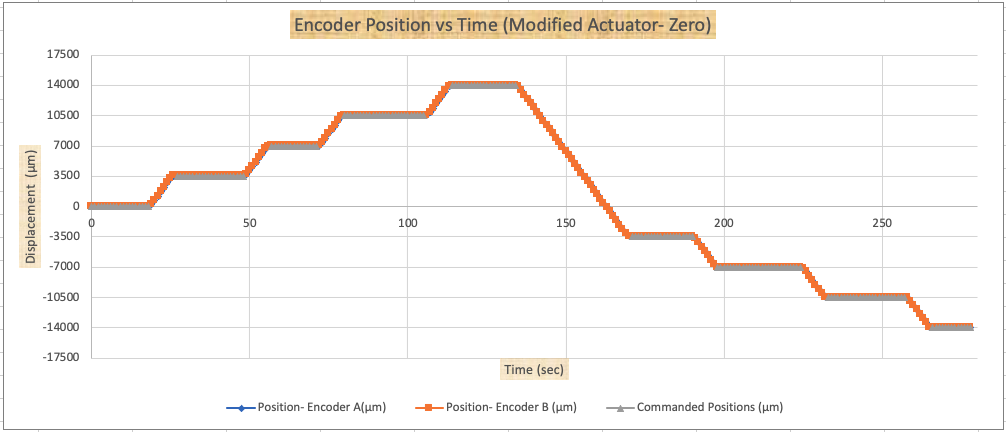
\includegraphics[width=5.98958in]{jira_imgs/4114.png}

}
\begin{tabular}{p{2cm}p{14cm}}
\toprule
Step 37 & Step Execution Status: \textbf{ Pass } \\ \hline
\end{tabular}
 Description \\
{\footnotesize
Record the actual displacement as measured by the internal encoder using
copley software.

}
\hdashrule[0.5ex]{\textwidth}{1pt}{3mm}
  Expected Result \\
{\footnotesize
Actual displacement measured by the internal encoder recorded in the
Copley Software.

}
\hdashrule[0.5ex]{\textwidth}{1pt}{3mm}
  Actual Result \\
{\footnotesize
The Active Load Position reported by the Copley Control Software could
not be exported. However, we confirmed the absolute position movements
as reported by the Copley Control Software.

}
\begin{tabular}{p{2cm}p{14cm}}
\toprule
Step 38 & Step Execution Status: \textbf{ Pass } \\ \hline
\end{tabular}
 Description \\
{\footnotesize
Compare the internal linear encoder measurement with the average of the
two external linear encoder measurements.

}
\hdashrule[0.5ex]{\textwidth}{1pt}{3mm}
  Expected Result \\
{\footnotesize
\textbf{The large-scale accuracy error \textless{}= 17um.}

}
\hdashrule[0.5ex]{\textwidth}{1pt}{3mm}
  Actual Result \\
{\footnotesize
There were some variations to the load while the actuator was moved.
Therefore, load compensation was applied similar to MOOG's procedure. As
a result, the average accuracy error can be seen below in orange:\\
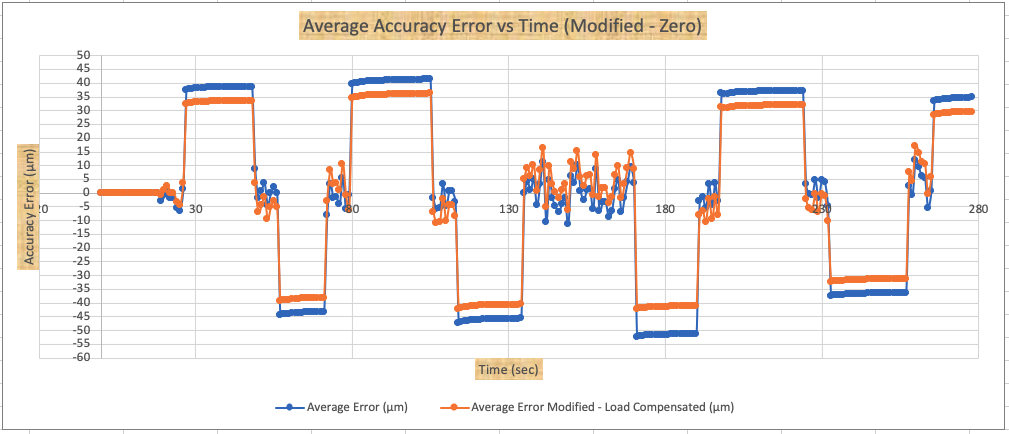
\includegraphics[width=5.98958in]{jira_imgs/4113.png}By analyzing the
data from the external linear encoder measurements, the large-scale
accuracy error was seen to be mostly within \textless{}= 17um with load
compensation. This can be seen in the Average Accuracy Error vs. Time
(Modified - Zero) plot in the previous step. There were some outliers
noted, but this was expected as MOOG's original report showed noise on
the load cell and the external encoders. Although load compensation was
applied, there were still some errors that can be attributed to the
noise. Since this does not impact our ability to meet the hexapod level
requirement, this was marked as passed.

}
\begin{tabular}{p{2cm}p{14cm}}
\toprule
Step 39 & Step Execution Status: \textbf{ Pass } \\ \hline
\end{tabular}
 Description \\
{\footnotesize
Restart at the zero position.

}
\hdashrule[0.5ex]{\textwidth}{1pt}{3mm}
  Test Data \\
 {\footnotesize
\textbf{Note:~}Command the actuator to the absolute zero position.

}
\hdashrule[0.5ex]{\textwidth}{1pt}{3mm}
  Expected Result \\
{\footnotesize
Actuator positioned at its center of stroke position ~confirmed by
encoder reading in the LabView.

}
\hdashrule[0.5ex]{\textwidth}{1pt}{3mm}
  Actual Result \\
{\footnotesize
The actuator was commanded back to the absolute zero position.

}
\begin{tabular}{p{2cm}p{14cm}}
\toprule
Step 40 & Step Execution Status: \textbf{ Pass } \\ \hline
\end{tabular}
 Description \\
{\footnotesize
With ``zero'' load applied to the actuator, command the following moves
using the copley software and the control box in absolute mode: +100um,
+200um, +300um, +400um, -100um, -200um, -300um, -400um.

}
\hdashrule[0.5ex]{\textwidth}{1pt}{3mm}
  Expected Result \\
{\footnotesize
All moves should move in the commanded direction.

}
\hdashrule[0.5ex]{\textwidth}{1pt}{3mm}
  Actual Result \\
{\footnotesize
+100um = 100000 counts\\
Active Load Position = 0.1002mm\\[2\baselineskip]+200um = 200000
counts\\
Active Load Position = 0.2002mm\\[2\baselineskip]+300um = 300000
counts\\
Active Load Position = 0.3000mm\\[2\baselineskip]+400um = 400000
counts\\
Active Load Position = 0.3999mm\\[2\baselineskip]-100um = -100000
counts\\
Active Load Position = -0.0999mm\\[2\baselineskip]-200um = -200000
counts\\
Active Load Position = -0.1999mm\\[2\baselineskip]-300um =-300000
counts\\
Active Load Position = -0.2999mm\\[2\baselineskip]-400um = -400000
counts\\
Active Load Position = -0.3999mm

}
\begin{tabular}{p{2cm}p{14cm}}
\toprule
Step 41 & Step Execution Status: \textbf{ Pass } \\ \hline
\end{tabular}
 Description \\
{\footnotesize
Record the actual displacement as measured by average of ~the two
external encoder as Labview graph (Displacement vs Time).

}
\hdashrule[0.5ex]{\textwidth}{1pt}{3mm}
  Expected Result \\
{\footnotesize
Actual displacement measured by the average of the two external encoders
~recorded in the LabView graph.

}
\hdashrule[0.5ex]{\textwidth}{1pt}{3mm}
  Actual Result \\
{\footnotesize
The recorded data was exported from LabView into the~Accuracy-Small
Scale sheet of the \emph{Accuracy Test Results -Modified vs
Unmodified.xlsx} excel document. The plotted values can be seen below
where the blue line represents the average displacement of the external
encoders and the orange line represents the commanded position:\\
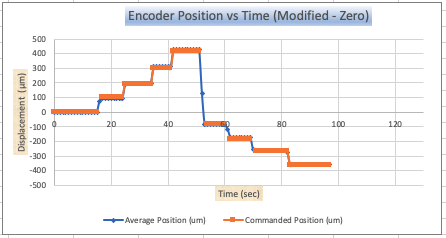
\includegraphics[width=5.98958in]{jira_imgs/4112.png}

}
\begin{tabular}{p{2cm}p{14cm}}
\toprule
Step 42 & Step Execution Status: \textbf{ Pass } \\ \hline
\end{tabular}
 Description \\
{\footnotesize
Record the actual displacement as measured by the internal encoder using
copley software.

}
\hdashrule[0.5ex]{\textwidth}{1pt}{3mm}
  Expected Result \\
{\footnotesize
Actual displacement measured by the internal encoder recorded in the
Copley Software.

}
\hdashrule[0.5ex]{\textwidth}{1pt}{3mm}
  Actual Result \\
{\footnotesize
The Active Load Position reported by the Copley Control Software could
not be exported. However, we monitored the absolute position movements
at the time of the test as reported by the Copley Control Software.

}
\begin{tabular}{p{2cm}p{14cm}}
\toprule
Step 43 & Step Execution Status: \textbf{ Pass } \\ \hline
\end{tabular}
 Description \\
{\footnotesize
Compare the internal linear encoder measurement with the average of the
two external linear encoder measurements.

}
\hdashrule[0.5ex]{\textwidth}{1pt}{3mm}
  Expected Result \\
{\footnotesize
\textbf{The small-scale accuracy error \textless{}= 20um.}

}
\hdashrule[0.5ex]{\textwidth}{1pt}{3mm}
  Actual Result \\
{\footnotesize
As seen in the plot attached to Step 41, there was some variation of
load seen at the time of the test. Therefore, load compensation was
applied similar to MOOG's procedure. As a result, the average accuracy
error can be seen below in blue:\\
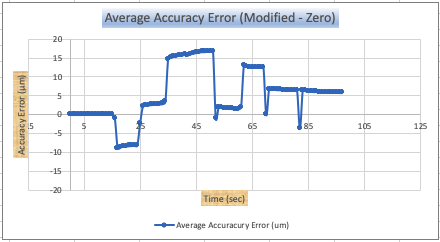
\includegraphics[width=5.98958in]{jira_imgs/4111.png}\\
As seen by the plot, the average accuracy error was within 20um. This
Average Accuracy Error (Modified - Zero) plot can be found on
the~Accuracy- Small Scale~sheet of the\emph{~Accuracy Test Results
-Modified vs Unmodifed.xlsx} document.

}
\begin{tabular}{p{2cm}p{14cm}}
\toprule
Step 44 & Step Execution Status: \textbf{ Pass } \\ \hline
\end{tabular}
 Description \\
{\footnotesize
Press Stop button in the VI file front panel to stop reading of the
components.

}
\hdashrule[0.5ex]{\textwidth}{1pt}{3mm}
  Expected Result \\
{\footnotesize
Graphs in the front panel of the VI file becomes static.

}
\hdashrule[0.5ex]{\textwidth}{1pt}{3mm}
  Actual Result \\
{\footnotesize
The LabView VI's were stopped.

}
\begin{tabular}{p{2cm}p{14cm}}
\toprule
Step 45 & Step Execution Status: \textbf{ Pass } \\ \hline
\end{tabular}
 Description \\
{\footnotesize
Check if all the test results are recorded in excel spreadsheets.

}
\hdashrule[0.5ex]{\textwidth}{1pt}{3mm}
  Expected Result \\
{\footnotesize
Test Results are recorded in the excel spreadsheets residing in the
LabView Folder directory.

}
\hdashrule[0.5ex]{\textwidth}{1pt}{3mm}
  Actual Result \\
{\footnotesize
All test results have been recorded and attached to the previous
steps.‚Äã‚Äã‚Äã‚Äã

}
\begin{tabular}{p{2cm}p{14cm}}
\toprule
Step 46 & Step Execution Status: \textbf{ Not Executed } \\ \hline
\end{tabular}
 Description \\
{\footnotesize
Close all the Labview VI files.

}
\hdashrule[0.5ex]{\textwidth}{1pt}{3mm}
  Test Data \\
 {\footnotesize
\textbf{Note:~}Labview can be left open in order to continue to the next
test. However, it may be necessary to reset the application before
starting the next test.

}
\hdashrule[0.5ex]{\textwidth}{1pt}{3mm}
  Expected Result \\
{\footnotesize
All the VI files are closed and Labview 2021 application window closes.

}
\hdashrule[0.5ex]{\textwidth}{1pt}{3mm}
  Actual Result \\
{\footnotesize
The LabView VI's were stopped, but not closed.

}

\paragraph{ LVV-T2435 - Hexapod - Actuator Repeatability Test }\mbox{}\\

Version \textbf{1}.
Status \textbf{Approved}.
Open  \href{https://jira.lsstcorp.org/secure/Tests.jspa#/testCase/LVV-T2435}{\textit{ LVV-T2435 } }
test case in Jira.

The objective of this test case will be to re-verify the hexapod
actuator repeatability requirements as stated in \citeds{LTS-206}. This will be
done by repeating a series of moves in order to verify that the
deviation between the sets of moves is not greater than 5um.~

\textbf{ Preconditions}:\\


Execution status: {\bf Pass }

Final comment:\\Similar to the execution of this test with the unmodified actuator, the
repeatability was determined by observing the measured displacement of
the actuator after completing a move and settle. As seen in the final
comparison of results in the
\href{https://docushare.lsst.org/docushare/dsweb/Services/Document-55071}{\emph{Repeatibility
Test Results -Modified vs UnModified.xlsx}} document, both the modified
and unmodified actuator had a repeatibility of less than 5um.\\
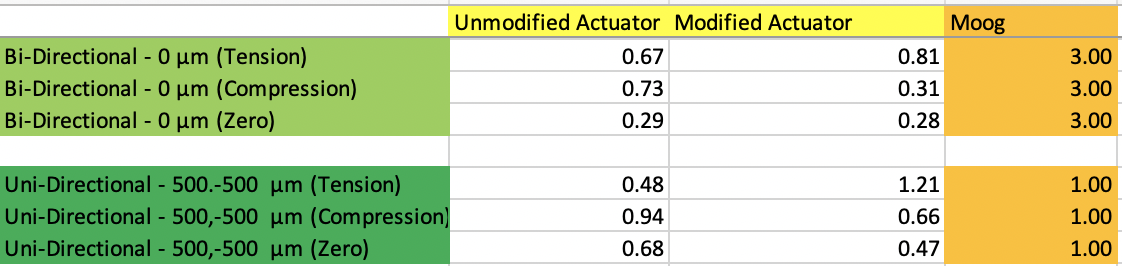
\includegraphics[width=4.42708in]{jira_imgs/4106.png}


Detailed steps results:

\begin{tabular}{p{2cm}p{14cm}}
\toprule
Step 0.4 & Step Execution Status: \textbf{ Not Executed } \\ \hline
\end{tabular}
 Description \\
{\footnotesize
Start at a random actuator stroke position sufficiently away from the
software stroke limits.

}
\hdashrule[0.5ex]{\textwidth}{1pt}{3mm}
  Test Data \\
 {\footnotesize
\textbf{Note:~}The actuator stroke from hard stop to hard stop is
+/-19.36mm. The minimum amount required to meet hexapod range
requirements is +/-16.02mm.

}
\hdashrule[0.5ex]{\textwidth}{1pt}{3mm}
  Expected Result \\
{\footnotesize
Appropriate actuator stroke-position selected for the test.~

}
\hdashrule[0.5ex]{\textwidth}{1pt}{3mm}
  Actual Result \\
{\footnotesize
The actuator was positioned at the center stroke position continuing
from the last test and so this step was skipped.

}
\begin{tabular}{p{2cm}p{14cm}}
\toprule
Step 0.4 & Step Execution Status: \textbf{ Not Executed } \\ \hline
\end{tabular}
 Description \\
{\footnotesize
Start at a random actuator stroke position sufficiently away from the
software stroke limits.

}
\hdashrule[0.5ex]{\textwidth}{1pt}{3mm}
  Test Data \\
 {\footnotesize
\textbf{Note:~}The actuator stroke from hard stop to hard stop is
+/-19.36mm. The minimum amount required to meet hexapod range
requirements is +/-16.02mm.

}
\hdashrule[0.5ex]{\textwidth}{1pt}{3mm}
  Expected Result \\
{\footnotesize
Appropriate actuator stroke-position selected for the test.~

}
\hdashrule[0.5ex]{\textwidth}{1pt}{3mm}
  Actual Result \\
{\footnotesize

}
\begin{tabular}{p{2cm}p{14cm}}
\toprule
Step 0.4 & Step Execution Status: \textbf{ Not Executed } \\ \hline
\end{tabular}
 Description \\
{\footnotesize
Start at a random actuator stroke position sufficiently away from the
software stroke limits.

}
\hdashrule[0.5ex]{\textwidth}{1pt}{3mm}
  Test Data \\
 {\footnotesize
\textbf{Note:~}The actuator stroke from hard stop to hard stop is
+/-19.36mm. The minimum amount required to meet hexapod range
requirements is +/-16.02mm.

}
\hdashrule[0.5ex]{\textwidth}{1pt}{3mm}
  Expected Result \\
{\footnotesize
Appropriate actuator stroke-position selected for the test.~

}
\hdashrule[0.5ex]{\textwidth}{1pt}{3mm}
  Actual Result \\
{\footnotesize
The actuator was positioned at the center stroke position continuing
from the last test and so this step was skipped.

}
\begin{tabular}{p{2cm}p{14cm}}
\toprule
Step 0.5 & Step Execution Status: \textbf{ Pass } \\ \hline
\end{tabular}
 Description \\
{\footnotesize
Apply a {15kN tension}⁠ load by using the LabView function to apply the
appropriate voltage values to the compression and tension air valves.

}
\hdashrule[0.5ex]{\textwidth}{1pt}{3mm}
  Test Data \\
 {\footnotesize
{\textbf{Note:}}

\begin{itemize}
\tightlist
\item
  {Tension test: Set Channel 1 = 2.19V and Channel 0 = 0V}
\item
  Zero Load test: Set Channel 1 = Channel 0 = 0V \textbf{~}
\item
  Compression test - Set Channel 1 = 0V and Channel 0 = 2.19V
\end{itemize}

}
\hdashrule[0.5ex]{\textwidth}{1pt}{3mm}
  Expected Result \\
{\footnotesize
The actuator has {15kN tension}⁠ load applied.

}
\hdashrule[0.5ex]{\textwidth}{1pt}{3mm}
  Actual Result \\
{\footnotesize
The tension force was applied by setting Channel 1 = 2.19V

}
\begin{tabular}{p{2cm}p{14cm}}
\toprule
Step 0.5 & Step Execution Status: \textbf{ Pass } \\ \hline
\end{tabular}
 Description \\
{\footnotesize
Apply a {zero}⁠ load by using the LabView function to apply the
appropriate voltage values to the compression and tension air valves.

}
\hdashrule[0.5ex]{\textwidth}{1pt}{3mm}
  Test Data \\
 {\footnotesize
{\textbf{Note:}}

\begin{itemize}
\tightlist
\item
  {Tension test: Set Channel 1 = 2.19V and Channel 0 = 0V}
\item
  Zero Load test: Set Channel 1 = Channel 0 = 0V \textbf{~}
\item
  Compression test - Set Channel 1 = 0V and Channel 0 = 2.19V
\end{itemize}

}
\hdashrule[0.5ex]{\textwidth}{1pt}{3mm}
  Expected Result \\
{\footnotesize
The actuator has {zero}⁠ load applied.

}
\hdashrule[0.5ex]{\textwidth}{1pt}{3mm}
  Actual Result \\
{\footnotesize
A zero load was applied by setting both channels to 0V.

}
\begin{tabular}{p{2cm}p{14cm}}
\toprule
Step 0.5 & Step Execution Status: \textbf{ Pass } \\ \hline
\end{tabular}
 Description \\
{\footnotesize
Apply a {15kN compression}⁠ load by using the LabView function to apply
the appropriate voltage values to the compression and tension air
valves.

}
\hdashrule[0.5ex]{\textwidth}{1pt}{3mm}
  Test Data \\
 {\footnotesize
{\textbf{Note:}}

\begin{itemize}
\tightlist
\item
  {Tension test: Set Channel 1 = 2.19V and Channel 0 = 0V}
\item
  Zero Load test: Set Channel 1 = Channel 0 = 0V \textbf{~}
\item
  Compression test - Set Channel 1 = 0V and Channel 0 = 2.19V
\end{itemize}

}
\hdashrule[0.5ex]{\textwidth}{1pt}{3mm}
  Expected Result \\
{\footnotesize
The actuator has {15kN compression}⁠ load applied.

}
\hdashrule[0.5ex]{\textwidth}{1pt}{3mm}
  Actual Result \\
{\footnotesize
The compression force was applied by setting Channel 0 = 2.19V

}
\begin{tabular}{p{2cm}p{14cm}}
\toprule
Step 0.6 & Step Execution Status: \textbf{ Pass } \\ \hline
\end{tabular}
 Description \\
{\footnotesize
Command the actuator to move to the absolute positions of +500um, 0um,
-500um, and then 0um.

}
\hdashrule[0.5ex]{\textwidth}{1pt}{3mm}
  Expected Result \\
{\footnotesize
The actuator moves to within 5um of the commanded absolute positions.

}
\hdashrule[0.5ex]{\textwidth}{1pt}{3mm}
  Actual Result \\
{\footnotesize
The sequence of moves were executed while Labview recorded the
displacement of the encoders.

}
\begin{tabular}{p{2cm}p{14cm}}
\toprule
Step 0.6 & Step Execution Status: \textbf{ Pass } \\ \hline
\end{tabular}
 Description \\
{\footnotesize
Command the actuator to move to the absolute positions of +500um, 0um,
-500um, and then 0um.

}
\hdashrule[0.5ex]{\textwidth}{1pt}{3mm}
  Expected Result \\
{\footnotesize
The actuator moves to within 5um of the commanded absolute positions.

}
\hdashrule[0.5ex]{\textwidth}{1pt}{3mm}
  Actual Result \\
{\footnotesize
The sequence of moves were executed while Labview recorded the
displacement of the encoders.

}
\begin{tabular}{p{2cm}p{14cm}}
\toprule
Step 0.6 & Step Execution Status: \textbf{ Pass } \\ \hline
\end{tabular}
 Description \\
{\footnotesize
Command the actuator to move to the absolute positions of +500um, 0um,
-500um, and then 0um.

}
\hdashrule[0.5ex]{\textwidth}{1pt}{3mm}
  Expected Result \\
{\footnotesize
The actuator moves to within 5um of the commanded absolute positions.

}
\hdashrule[0.5ex]{\textwidth}{1pt}{3mm}
  Actual Result \\
{\footnotesize
The sequence of moves were executed while Labview recorded the
displacement of the encoders.

}
\begin{tabular}{p{2cm}p{14cm}}
\toprule
Step 0.7 & Step Execution Status: \textbf{ Pass } \\ \hline
\end{tabular}
 Description \\
{\footnotesize
Command the actuator to move to the absolute positions of +500um, 0um,
-500um, and then 0um.

}
\hdashrule[0.5ex]{\textwidth}{1pt}{3mm}
  Expected Result \\
{\footnotesize
The actuator moves to within 5um of the commanded absolute positions.

}
\hdashrule[0.5ex]{\textwidth}{1pt}{3mm}
  Actual Result \\
{\footnotesize
The sequence of moves were executed while Labview recorded the
displacement of the encoders.

}
\begin{tabular}{p{2cm}p{14cm}}
\toprule
Step 0.7 & Step Execution Status: \textbf{ Pass } \\ \hline
\end{tabular}
 Description \\
{\footnotesize
Command the actuator to move to the absolute positions of +500um, 0um,
-500um, and then 0um.

}
\hdashrule[0.5ex]{\textwidth}{1pt}{3mm}
  Expected Result \\
{\footnotesize
The actuator moves to within 5um of the commanded absolute positions.

}
\hdashrule[0.5ex]{\textwidth}{1pt}{3mm}
  Actual Result \\
{\footnotesize
The sequence of moves were executed while Labview recorded the
displacement of the encoders.

}
\begin{tabular}{p{2cm}p{14cm}}
\toprule
Step 0.7 & Step Execution Status: \textbf{ Pass } \\ \hline
\end{tabular}
 Description \\
{\footnotesize
Command the actuator to move to the absolute positions of +500um, 0um,
-500um, and then 0um.

}
\hdashrule[0.5ex]{\textwidth}{1pt}{3mm}
  Expected Result \\
{\footnotesize
The actuator moves to within 5um of the commanded absolute positions.

}
\hdashrule[0.5ex]{\textwidth}{1pt}{3mm}
  Actual Result \\
{\footnotesize
The sequence of moves were executed while Labview recorded the
displacement of the encoders.

}
\begin{tabular}{p{2cm}p{14cm}}
\toprule
Step 0.8 & Step Execution Status: \textbf{ Pass } \\ \hline
\end{tabular}
 Description \\
{\footnotesize
Command the actuator to move to the absolute positions of +500um, 0um,
-500um, and then 0um.

}
\hdashrule[0.5ex]{\textwidth}{1pt}{3mm}
  Expected Result \\
{\footnotesize
The actuator moves to within 5um of the commanded absolute positions.

}
\hdashrule[0.5ex]{\textwidth}{1pt}{3mm}
  Actual Result \\
{\footnotesize
The sequence of moves were executed while Labview recorded the
displacement of the encoders.

}
\begin{tabular}{p{2cm}p{14cm}}
\toprule
Step 0.8 & Step Execution Status: \textbf{ Pass } \\ \hline
\end{tabular}
 Description \\
{\footnotesize
Command the actuator to move to the absolute positions of +500um, 0um,
-500um, and then 0um.

}
\hdashrule[0.5ex]{\textwidth}{1pt}{3mm}
  Expected Result \\
{\footnotesize
The actuator moves to within 5um of the commanded absolute positions.

}
\hdashrule[0.5ex]{\textwidth}{1pt}{3mm}
  Actual Result \\
{\footnotesize
The sequence of moves were executed while Labview recorded the
displacement of the encoders.

}
\begin{tabular}{p{2cm}p{14cm}}
\toprule
Step 0.8 & Step Execution Status: \textbf{ Pass } \\ \hline
\end{tabular}
 Description \\
{\footnotesize
Command the actuator to move to the absolute positions of +500um, 0um,
-500um, and then 0um.

}
\hdashrule[0.5ex]{\textwidth}{1pt}{3mm}
  Expected Result \\
{\footnotesize
The actuator moves to within 5um of the commanded absolute positions.

}
\hdashrule[0.5ex]{\textwidth}{1pt}{3mm}
  Actual Result \\
{\footnotesize
The sequence of moves were executed while Labview recorded the
displacement of the encoders.

}
\begin{tabular}{p{2cm}p{14cm}}
\toprule
Step 0.9 & Step Execution Status: \textbf{ Pass } \\ \hline
\end{tabular}
 Description \\
{\footnotesize
Command the actuator to move to the absolute positions of +500um, 0um,
-500um, and then 0um.

}
\hdashrule[0.5ex]{\textwidth}{1pt}{3mm}
  Expected Result \\
{\footnotesize
The actuator moves to within 5um of the commanded absolute positions.

}
\hdashrule[0.5ex]{\textwidth}{1pt}{3mm}
  Actual Result \\
{\footnotesize
The sequence of moves were executed while Labview recorded the
displacement of the encoders.

}
\begin{tabular}{p{2cm}p{14cm}}
\toprule
Step 0.9 & Step Execution Status: \textbf{ Pass } \\ \hline
\end{tabular}
 Description \\
{\footnotesize
Command the actuator to move to the absolute positions of +500um, 0um,
-500um, and then 0um.

}
\hdashrule[0.5ex]{\textwidth}{1pt}{3mm}
  Expected Result \\
{\footnotesize
The actuator moves to within 5um of the commanded absolute positions.

}
\hdashrule[0.5ex]{\textwidth}{1pt}{3mm}
  Actual Result \\
{\footnotesize
The sequence of moves were executed while Labview recorded the
displacement of the encoders.

}
\begin{tabular}{p{2cm}p{14cm}}
\toprule
Step 0.9 & Step Execution Status: \textbf{ Pass } \\ \hline
\end{tabular}
 Description \\
{\footnotesize
Command the actuator to move to the absolute positions of +500um, 0um,
-500um, and then 0um.

}
\hdashrule[0.5ex]{\textwidth}{1pt}{3mm}
  Expected Result \\
{\footnotesize
The actuator moves to within 5um of the commanded absolute positions.

}
\hdashrule[0.5ex]{\textwidth}{1pt}{3mm}
  Actual Result \\
{\footnotesize
The sequence of moves were executed while Labview recorded the
displacement of the encoders.

}
\begin{tabular}{p{2cm}p{14cm}}
\toprule
Step 1.0 & Step Execution Status: \textbf{ Pass } \\ \hline
\end{tabular}
 Description \\
{\footnotesize
Command the actuator to move to the absolute positions of +500um, 0um,
-500um, and then 0um.

}
\hdashrule[0.5ex]{\textwidth}{1pt}{3mm}
  Expected Result \\
{\footnotesize
The actuator moves to within 5um of the commanded absolute positions.

}
\hdashrule[0.5ex]{\textwidth}{1pt}{3mm}
  Actual Result \\
{\footnotesize
The sequence of moves were executed while Labview recorded the
displacement of the encoders.

}
\begin{tabular}{p{2cm}p{14cm}}
\toprule
Step 1.0 & Step Execution Status: \textbf{ Pass } \\ \hline
\end{tabular}
 Description \\
{\footnotesize
Command the actuator to move to the absolute positions of +500um, 0um,
-500um, and then 0um.

}
\hdashrule[0.5ex]{\textwidth}{1pt}{3mm}
  Expected Result \\
{\footnotesize
The actuator moves to within 5um of the commanded absolute positions.

}
\hdashrule[0.5ex]{\textwidth}{1pt}{3mm}
  Actual Result \\
{\footnotesize
The sequence of moves were executed while Labview recorded the
displacement of the encoders.

}
\begin{tabular}{p{2cm}p{14cm}}
\toprule
Step 1.0 & Step Execution Status: \textbf{ Pass } \\ \hline
\end{tabular}
 Description \\
{\footnotesize
Command the actuator to move to the absolute positions of +500um, 0um,
-500um, and then 0um.

}
\hdashrule[0.5ex]{\textwidth}{1pt}{3mm}
  Expected Result \\
{\footnotesize
The actuator moves to within 5um of the commanded absolute positions.

}
\hdashrule[0.5ex]{\textwidth}{1pt}{3mm}
  Actual Result \\
{\footnotesize
The sequence of moves were executed while Labview recorded the
displacement of the encoders.

}
\begin{tabular}{p{2cm}p{14cm}}
\toprule
Step 1.1 & Step Execution Status: \textbf{ Pass } \\ \hline
\end{tabular}
 Description \\
{\footnotesize
Record the results from all three sets of tests.

}
\hdashrule[0.5ex]{\textwidth}{1pt}{3mm}
  Test Data \\
 {\footnotesize
\textbf{Note}: A script will be used to continuously pull the encoder
readings and export them into an Excel sheet.

}
\hdashrule[0.5ex]{\textwidth}{1pt}{3mm}
  Expected Result \\
{\footnotesize
The results of all the tests shows there are no errors in movements more
than 5um.~

}
\hdashrule[0.5ex]{\textwidth}{1pt}{3mm}
  Actual Result \\
{\footnotesize
The results of the first test in Tension can be seen below:\\
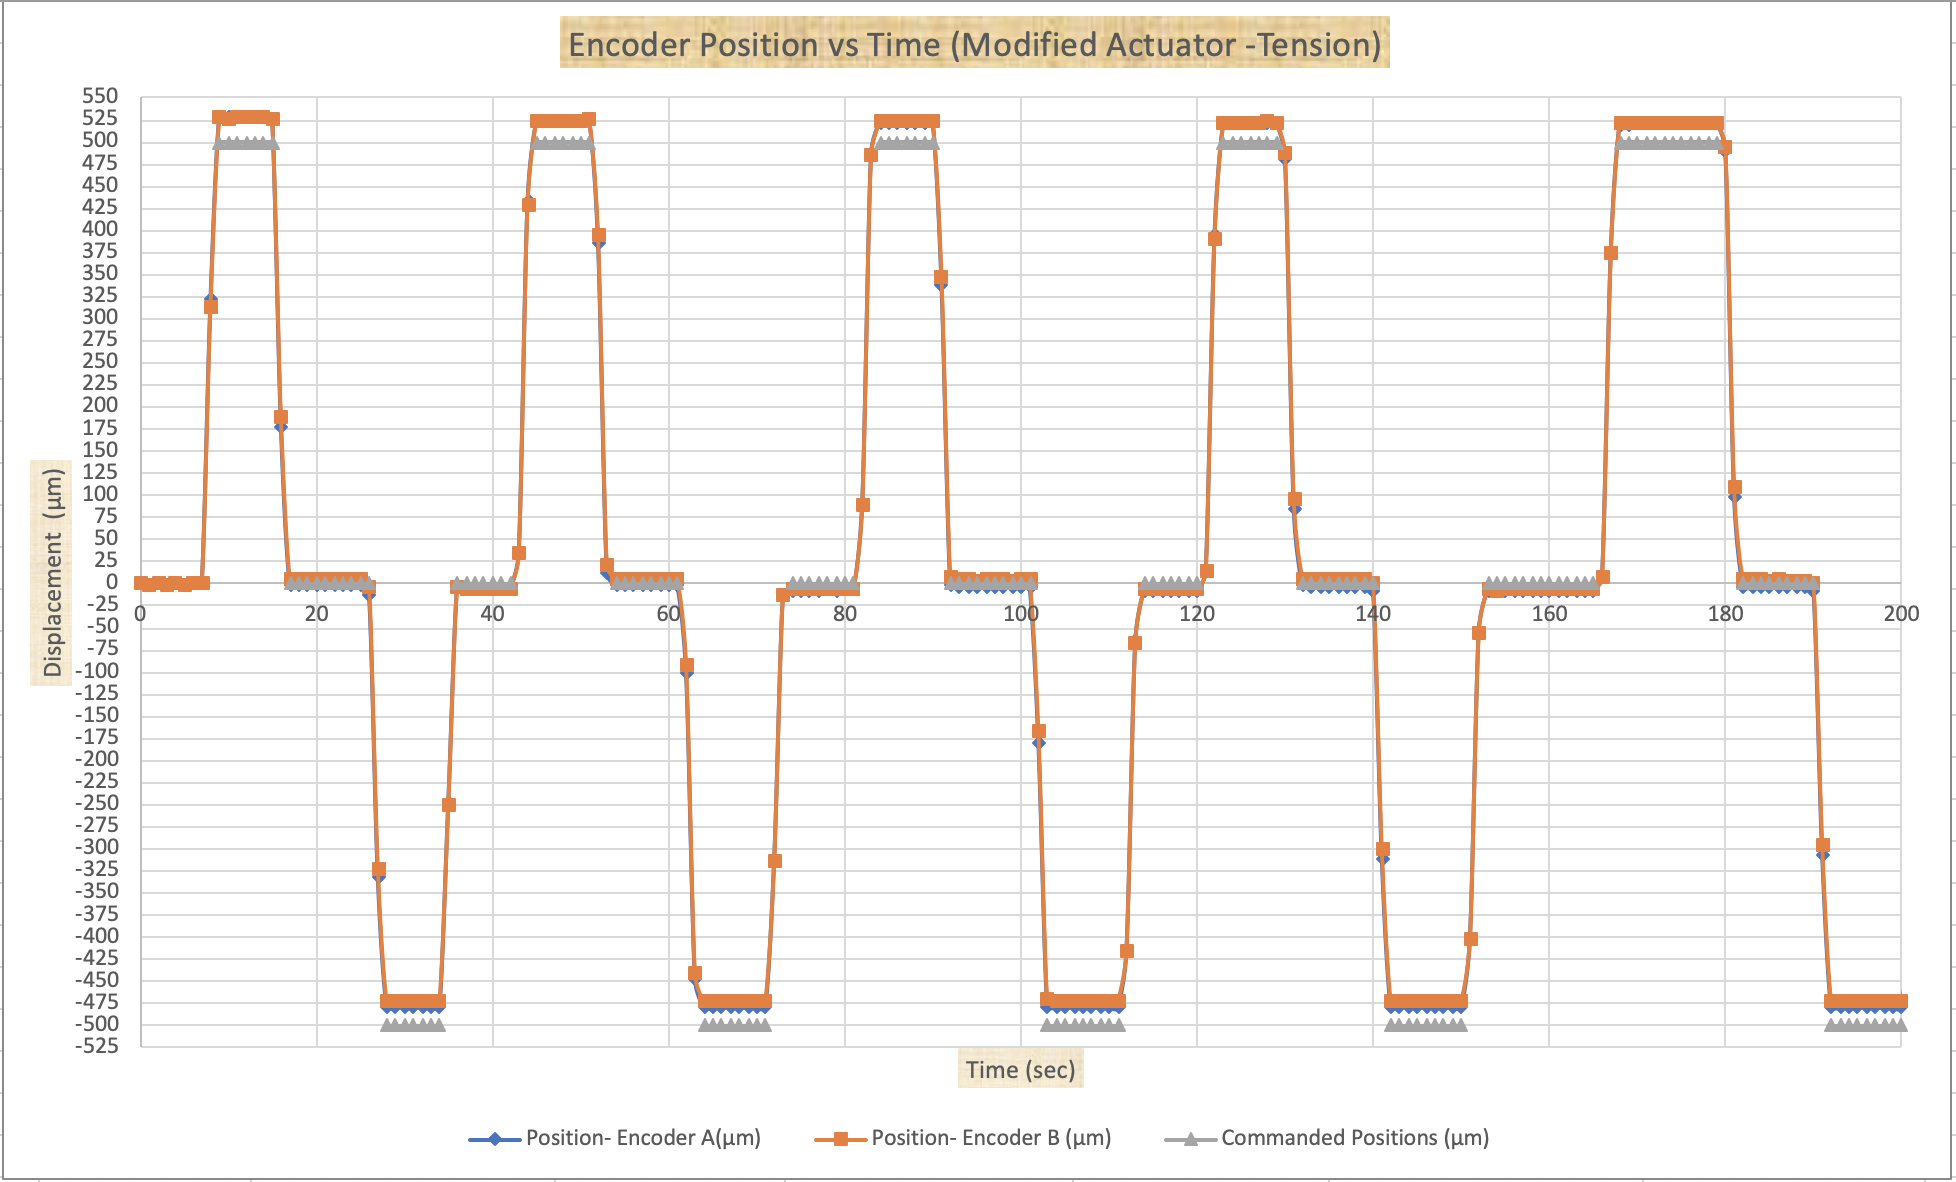
\includegraphics[width=5.98958in]{jira_imgs/4103.png}It can be seen in
general that the commanded moves were very repeatable, always being
fairly close to the previously visited position. This Encoder Position
vs Time (Modified Actuator- Tension) plot can be found in the
\emph{Repeatability Test Results -Modified vs Unmodified
Actuator.xlsx~}file

}
\begin{tabular}{p{2cm}p{14cm}}
\toprule
Step 1.1 & Step Execution Status: \textbf{ Pass } \\ \hline
\end{tabular}
 Description \\
{\footnotesize
Record the results from all three sets of tests.

}
\hdashrule[0.5ex]{\textwidth}{1pt}{3mm}
  Test Data \\
 {\footnotesize
\textbf{Note}: A script will be used to continuously pull the encoder
readings and export them into an Excel sheet.

}
\hdashrule[0.5ex]{\textwidth}{1pt}{3mm}
  Expected Result \\
{\footnotesize
The results of all the tests shows there are no errors in movements more
than 5um.~

}
\hdashrule[0.5ex]{\textwidth}{1pt}{3mm}
  Actual Result \\
{\footnotesize
The results of the second test with no load can be seen below:\\
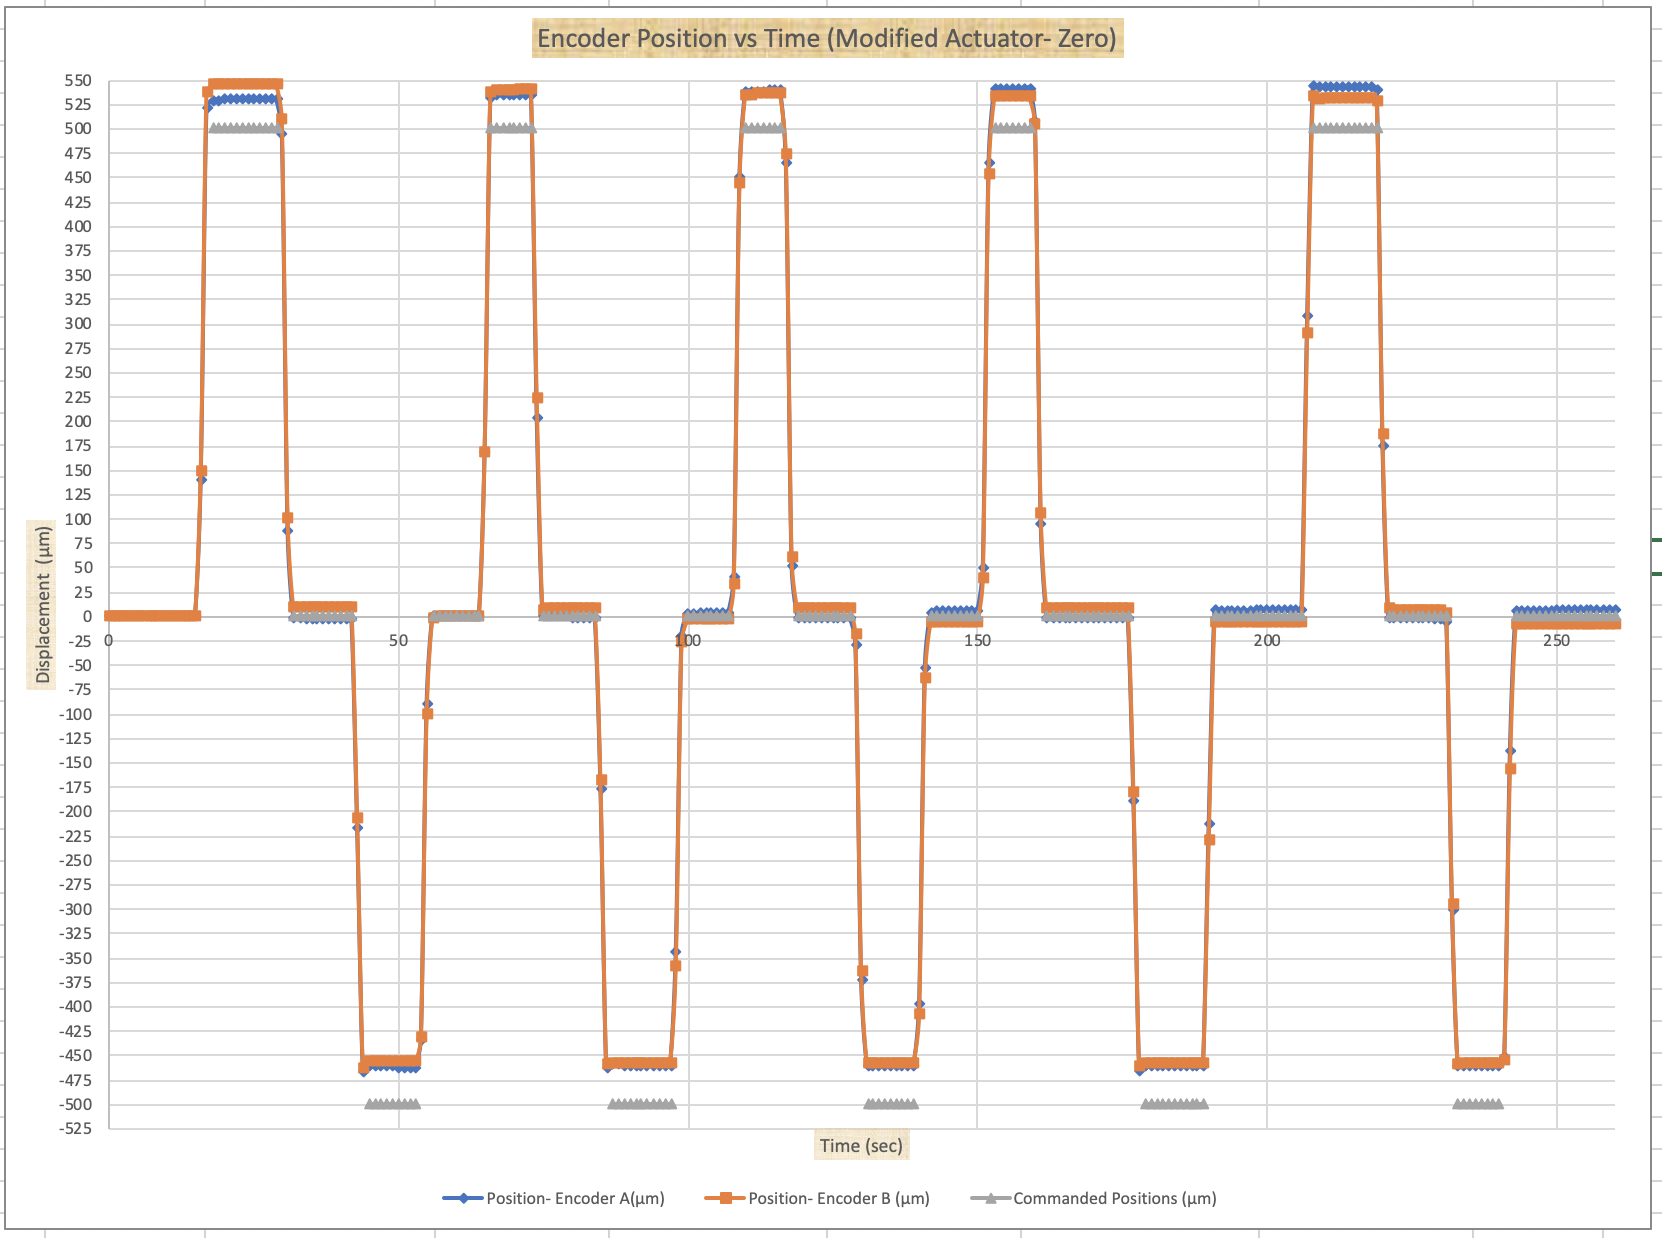
\includegraphics[width=5.98958in]{jira_imgs/4104.png}It can be seen in
general that the commanded moves were very repeatable, always being
fairly close to the previously visited position. This Encoder Position
vs Time (Modified Actuator- Zero) plot can be found in the
\emph{Repeatability Test Results -Modified vs Unmodified
Actuator.xlsx~}file

}
\begin{tabular}{p{2cm}p{14cm}}
\toprule
Step 1.1 & Step Execution Status: \textbf{ Pass } \\ \hline
\end{tabular}
 Description \\
{\footnotesize
Record the results from all three sets of tests.

}
\hdashrule[0.5ex]{\textwidth}{1pt}{3mm}
  Test Data \\
 {\footnotesize
\textbf{Note}: A script will be used to continuously pull the encoder
readings and export them into an Excel sheet.

}
\hdashrule[0.5ex]{\textwidth}{1pt}{3mm}
  Expected Result \\
{\footnotesize
The results of all the tests shows there are no errors in movements more
than 5um.~

}
\hdashrule[0.5ex]{\textwidth}{1pt}{3mm}
  Actual Result \\
{\footnotesize
The results of the third test in Compression can be seen below:\\
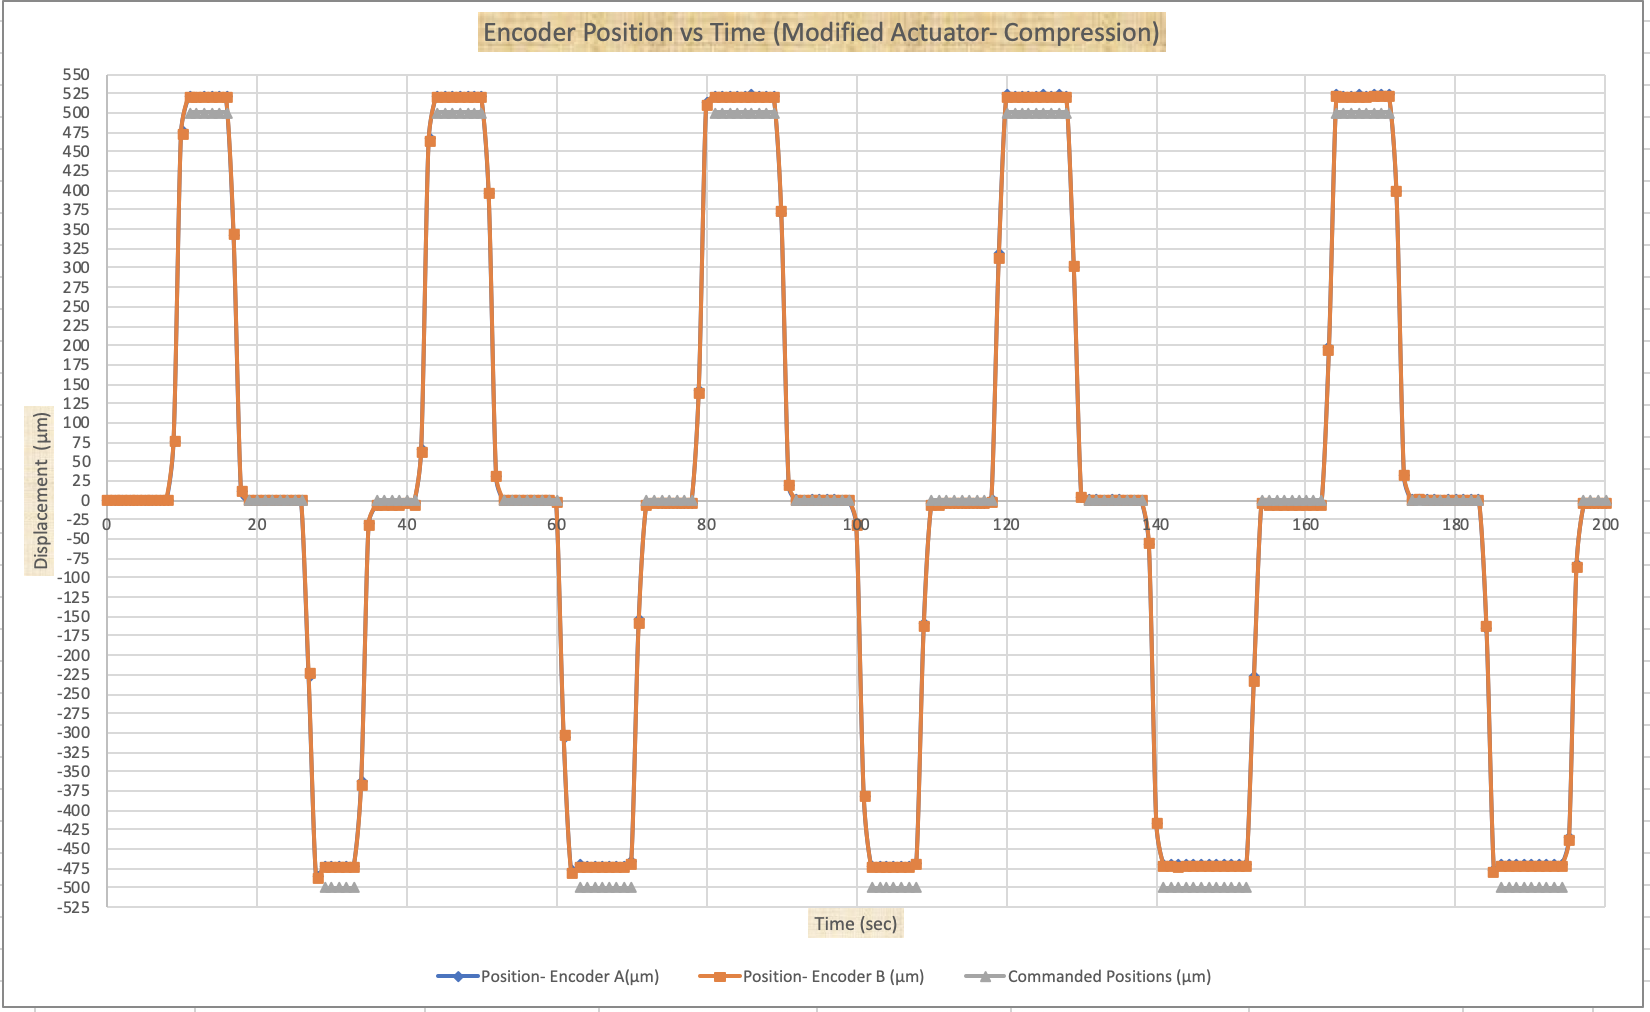
\includegraphics[width=5.98958in]{jira_imgs/4105.png}It can be seen in
general that the commanded moves were very repeatable, always being
fairly close to the previously visited position. This Encoder Position
vs Time (Modified Actuator- Compression) plot can be found in the
\emph{Repeatability Test Results -Modified vs Unmodified
Actuator.xlsx~}file

}
\begin{tabular}{p{2cm}p{14cm}}
\toprule
Step 1.1 & Step Execution Status: \textbf{ Pass } \\ \hline
\end{tabular}
 Description \\
{\footnotesize
Open Labview 2021 in the computer used for Test Setup.

}
\hdashrule[0.5ex]{\textwidth}{1pt}{3mm}
  Test Data \\
 {\footnotesize
The first three steps are conditional because these steps are included
as part of the Test Setup procedure and may not be necessary if LabView
is still open.

}
\hdashrule[0.5ex]{\textwidth}{1pt}{3mm}
  Expected Result \\
{\footnotesize
Labview 2021 opens successfully.

}
\hdashrule[0.5ex]{\textwidth}{1pt}{3mm}
  Actual Result \\
{\footnotesize
Labview was opened successfully.

}
\begin{tabular}{p{2cm}p{14cm}}
\toprule
Step 1.2 & Step Execution Status: \textbf{ Pass } \\ \hline
\end{tabular}
 Description \\
{\footnotesize
Run the following VI's:

\begin{itemize}
\tightlist
\item
  Encoder A (D13B) and Load Cell.vi
\item
  Encoder B (D0BD).vi
\end{itemize}

}
\hdashrule[0.5ex]{\textwidth}{1pt}{3mm}
  Expected Result \\
{\footnotesize
Front panel of VI's open without any error.

}
\hdashrule[0.5ex]{\textwidth}{1pt}{3mm}
  Actual Result \\
{\footnotesize
Labview was opened successfully.

}
\begin{tabular}{p{2cm}p{14cm}}
\toprule
Step 1.3 & Step Execution Status: \textbf{ Pass } \\ \hline
\end{tabular}
 Description \\
{\footnotesize
Click Run button on the block diagram toolbar of the Labview VI front
panel.

}
\hdashrule[0.5ex]{\textwidth}{1pt}{3mm}
  Expected Result \\
{\footnotesize
LabView VI and associated sub Vi runs successfully. The graphs should
start to be populated with data once the run button is pressed.

}
\hdashrule[0.5ex]{\textwidth}{1pt}{3mm}
  Actual Result \\
{\footnotesize
LabView was ran without any issue.‚Äã‚Äã‚Äã‚Äã

}
\begin{tabular}{p{2cm}p{14cm}}
\toprule
Step 2.1 & Step Execution Status: \textbf{ Pass } \\ \hline
\end{tabular}
 Description \\
{\footnotesize
Open Labview 2021 in the computer used for Test Setup.

}
\hdashrule[0.5ex]{\textwidth}{1pt}{3mm}
  Test Data \\
 {\footnotesize
The first three steps are conditional because these steps are included
as part of the Test Setup procedure and may not be necessary if LabView
is still open.

}
\hdashrule[0.5ex]{\textwidth}{1pt}{3mm}
  Expected Result \\
{\footnotesize
Labview 2021 opens successfully.

}
\hdashrule[0.5ex]{\textwidth}{1pt}{3mm}
  Actual Result \\
{\footnotesize
Labview was opened successfully.

}
\begin{tabular}{p{2cm}p{14cm}}
\toprule
Step 2.2 & Step Execution Status: \textbf{ Not Executed } \\ \hline
\end{tabular}
 Description \\
{\footnotesize
Close all the Labview VI files.

}
\hdashrule[0.5ex]{\textwidth}{1pt}{3mm}
  Test Data \\
 {\footnotesize
\textbf{Note:~}Labview can be left open in order to continue to the next
test. However, it may be necessary to reset the application before
starting the next test.

}
\hdashrule[0.5ex]{\textwidth}{1pt}{3mm}
  Expected Result \\
{\footnotesize
All the VI files are closed and Labview 2021 application window closes.

}
\hdashrule[0.5ex]{\textwidth}{1pt}{3mm}
  Actual Result \\
{\footnotesize
The LabView files were stopped, but were not closed.

}
\begin{tabular}{p{2cm}p{14cm}}
\toprule
Step 2.2 & Step Execution Status: \textbf{ Pass } \\ \hline
\end{tabular}
 Description \\
{\footnotesize
Run the following VI's:

\begin{itemize}
\tightlist
\item
  Encoder A (D13B) and Load Cell.vi
\item
  Encoder B (D0BD).vi
\end{itemize}

}
\hdashrule[0.5ex]{\textwidth}{1pt}{3mm}
  Expected Result \\
{\footnotesize
Front panel of VI's open without any error.

}
\hdashrule[0.5ex]{\textwidth}{1pt}{3mm}
  Actual Result \\
{\footnotesize
Labview was opened successfully.

}
\begin{tabular}{p{2cm}p{14cm}}
\toprule
Step 2.3 & Step Execution Status: \textbf{ Pass } \\ \hline
\end{tabular}
 Description \\
{\footnotesize
Click Run button on the block diagram toolbar of the Labview VI front
panel.

}
\hdashrule[0.5ex]{\textwidth}{1pt}{3mm}
  Expected Result \\
{\footnotesize
LabView VI and associated sub Vi runs successfully. The graphs should
start to be populated with data once the run button is pressed.

}
\hdashrule[0.5ex]{\textwidth}{1pt}{3mm}
  Actual Result \\
{\footnotesize
LabView was ran without any issue.‚Äã‚Äã‚Äã‚Äã

}
\begin{tabular}{p{2cm}p{14cm}}
\toprule
Step 3.1 & Step Execution Status: \textbf{ Pass } \\ \hline
\end{tabular}
 Description \\
{\footnotesize
Open Labview 2021 in the computer used for Test Setup.

}
\hdashrule[0.5ex]{\textwidth}{1pt}{3mm}
  Test Data \\
 {\footnotesize
The first three steps are conditional because these steps are included
as part of the Test Setup procedure and may not be necessary if LabView
is still open.

}
\hdashrule[0.5ex]{\textwidth}{1pt}{3mm}
  Expected Result \\
{\footnotesize
Labview 2021 opens successfully.

}
\hdashrule[0.5ex]{\textwidth}{1pt}{3mm}
  Actual Result \\
{\footnotesize
Labview was opened successfully.

}
\begin{tabular}{p{2cm}p{14cm}}
\toprule
Step 3.2 & Step Execution Status: \textbf{ Not Executed } \\ \hline
\end{tabular}
 Description \\
{\footnotesize
Close all the Labview VI files.

}
\hdashrule[0.5ex]{\textwidth}{1pt}{3mm}
  Test Data \\
 {\footnotesize
\textbf{Note:~}Labview can be left open in order to continue to the next
test. However, it may be necessary to reset the application before
starting the next test.

}
\hdashrule[0.5ex]{\textwidth}{1pt}{3mm}
  Expected Result \\
{\footnotesize
All the VI files are closed and Labview 2021 application window closes.

}
\hdashrule[0.5ex]{\textwidth}{1pt}{3mm}
  Actual Result \\
{\footnotesize
The LabView files were stopped, but were not closed.

}
\begin{tabular}{p{2cm}p{14cm}}
\toprule
Step 3.2 & Step Execution Status: \textbf{ Pass } \\ \hline
\end{tabular}
 Description \\
{\footnotesize
Run the following VI's:

\begin{itemize}
\tightlist
\item
  Encoder A (D13B) and Load Cell.vi
\item
  Encoder B (D0BD).vi
\end{itemize}

}
\hdashrule[0.5ex]{\textwidth}{1pt}{3mm}
  Expected Result \\
{\footnotesize
Front panel of VI's open without any error.

}
\hdashrule[0.5ex]{\textwidth}{1pt}{3mm}
  Actual Result \\
{\footnotesize
Labview was opened successfully.

}
\begin{tabular}{p{2cm}p{14cm}}
\toprule
Step 3.3 & Step Execution Status: \textbf{ Pass } \\ \hline
\end{tabular}
 Description \\
{\footnotesize
Click Run button on the block diagram toolbar of the Labview VI front
panel.

}
\hdashrule[0.5ex]{\textwidth}{1pt}{3mm}
  Expected Result \\
{\footnotesize
LabView VI and associated sub Vi runs successfully. The graphs should
start to be populated with data once the run button is pressed.

}
\hdashrule[0.5ex]{\textwidth}{1pt}{3mm}
  Actual Result \\
{\footnotesize
LabView was ran without any issue.

}
\begin{tabular}{p{2cm}p{14cm}}
\toprule
Step 4.2 & Step Execution Status: \textbf{ Not Executed } \\ \hline
\end{tabular}
 Description \\
{\footnotesize
Close all the Labview VI files.

}
\hdashrule[0.5ex]{\textwidth}{1pt}{3mm}
  Test Data \\
 {\footnotesize
\textbf{Note:~}Labview can be left open in order to continue to the next
test. However, it may be necessary to reset the application before
starting the next test.

}
\hdashrule[0.5ex]{\textwidth}{1pt}{3mm}
  Expected Result \\
{\footnotesize
All the VI files are closed and Labview 2021 application window closes.

}
\hdashrule[0.5ex]{\textwidth}{1pt}{3mm}
  Actual Result \\
{\footnotesize
The LabView files were stopped, but were not closed.

}

\paragraph{ LVV-T2431 - Hexapod - Actuator Accelerated Life Test }\mbox{}\\

Version \textbf{1}.
Status \textbf{Approved}.
Open  \href{https://jira.lsstcorp.org/secure/Tests.jspa#/testCase/LVV-T2431}{\textit{ LVV-T2431 } }
test case in Jira.

The objective of this test case will be to verify the actuator will
withstand at least a month's worth of operation by commanding it through
a repetitive sequence of motions.

\textbf{ Preconditions}:\\
In order to execute this test case, all other Hexapod re-verification
tests must be complete and the actuator should be connected to the
pneumatic cylinder.

Execution status: {\bf Pass }

Final comment:\\An initial sequence of 20 moves was performed and the actuator
temperature was seen to rise from 23.65degC to 28.5degC without any
indication of stopping. The operational limit of the actuator drive was
cited to be from 0 to 40degC. Therefore, we added a fan to prevent the
temperature from increasing beyond 30degC during the test. During the
tests, the temperature readings could not be exported while the
telemetry was being displayed in real time. Therefore, the temperature
telemetry was left on display to verify the temperature never reached
above 30degC. As a result of this test, the temperature never rose
beyond 30degC with the fan on the actuator and there were no obvious
damage/faults on the actuator.~


Detailed steps results:

\begin{tabular}{p{2cm}p{14cm}}
\toprule
Step 1 & Step Execution Status: \textbf{ Pass } \\ \hline
\end{tabular}
 Description \\
{\footnotesize
Open Labview 2021 in the computer used for Test Setup.

}
\hdashrule[0.5ex]{\textwidth}{1pt}{3mm}
  Test Data \\
 {\footnotesize
The first three steps are conditional because these steps are included
as part of the Test Setup procedure and may not be necessary if LabView
is still open.\\[4\baselineskip]

}
\hdashrule[0.5ex]{\textwidth}{1pt}{3mm}
  Expected Result \\
{\footnotesize
Labview 2021 opens successfully.

}
\hdashrule[0.5ex]{\textwidth}{1pt}{3mm}
  Actual Result \\
{\footnotesize
Labview was opened successfully.

}
\begin{tabular}{p{2cm}p{14cm}}
\toprule
Step 2 & Step Execution Status: \textbf{ Pass } \\ \hline
\end{tabular}
 Description \\
{\footnotesize
Run the following VI's:

\begin{itemize}
\tightlist
\item
  Encoder A (D13B) and Load Cell.vi
\item
  Encoder B (D0BD).vi
\end{itemize}

}
\hdashrule[0.5ex]{\textwidth}{1pt}{3mm}
  Expected Result \\
{\footnotesize
Front panel of VI's open without any error.

}
\hdashrule[0.5ex]{\textwidth}{1pt}{3mm}
  Actual Result \\
{\footnotesize
Labview was opened successfully.

}
\begin{tabular}{p{2cm}p{14cm}}
\toprule
Step 3 & Step Execution Status: \textbf{ Pass } \\ \hline
\end{tabular}
 Description \\
{\footnotesize
Click Run button on the on the block diagram toolbar of the Labview VI
front panel.

}
\hdashrule[0.5ex]{\textwidth}{1pt}{3mm}
  Expected Result \\
{\footnotesize
LabView VI and associated sub Vi runs successfully. The graphs should
start to be populated with data once the run button is pressed.

}
\hdashrule[0.5ex]{\textwidth}{1pt}{3mm}
  Actual Result \\
{\footnotesize
LabView was ran without any issue.‚Äã‚Äã‚Äã‚Äã

}
\begin{tabular}{p{2cm}p{14cm}}
\toprule
Step 4 & Step Execution Status: \textbf{ Pass } \\ \hline
\end{tabular}
 Description \\
{\footnotesize
Apply a +20kN load.

}
\hdashrule[0.5ex]{\textwidth}{1pt}{3mm}
  Test Data \\
 {\footnotesize
\textbf{Note:~}Set the tension valve to 2.92 V.

}
\hdashrule[0.5ex]{\textwidth}{1pt}{3mm}
  Expected Result \\
{\footnotesize
The LabView load graph( Time vs Load) shows 20 KN tension load has been
applied.

}
\hdashrule[0.5ex]{\textwidth}{1pt}{3mm}
  Actual Result \\
{\footnotesize
We were able to apply +20kN of force by setting Channel 1 = 2.92V

}
\begin{tabular}{p{2cm}p{14cm}}
\toprule
Step 5 & Step Execution Status: \textbf{ Pass } \\ \hline
\end{tabular}
 Description \\
{\footnotesize
Move the actuator through 20 cycles of the following command sequence
with 5 seconds between each move:\\[2\baselineskip]

\begin{longtable}[]{@{}ll@{}}
\toprule
Command \# & Absolute Position (mm)\tabularnewline
\midrule
\endhead
0 & 0\tabularnewline
1 & 8\tabularnewline
2 & 8.05\tabularnewline
3 & 8.06\tabularnewline
4 & 7.96\tabularnewline
5 & 7.92\tabularnewline
6 & 7.9\tabularnewline
7 & 7.92\tabularnewline
8 & 7.85\tabularnewline
9 & 7.8\tabularnewline
10 & 7.81\tabularnewline
11 & 7.84\tabularnewline
12 & 7.9\tabularnewline
13 & 7.98\tabularnewline
14 & 7.97\tabularnewline
15 & 8.02\tabularnewline
16 & 8.04\tabularnewline
17 & 8.08\tabularnewline
18 & 8.05\tabularnewline
19 & 8\tabularnewline
20 & 0\tabularnewline
\bottomrule
\end{longtable}

}
\hdashrule[0.5ex]{\textwidth}{1pt}{3mm}
  Test Data \\
 {\footnotesize
\textbf{Note:~}There is no need to simulate an entire year's worth of
testing. Therefore, the number of cycles can be reduced to a few days'
worth.

}
\hdashrule[0.5ex]{\textwidth}{1pt}{3mm}
  Expected Result \\
{\footnotesize
The actuator moves with no unexpected stoppages or failures and takes
around \_\_\_\_ with a total travel of 335mm. LabView Time vs Distance
graph shows the positions.~

}
\hdashrule[0.5ex]{\textwidth}{1pt}{3mm}
  Actual Result \\
{\footnotesize
Before applying load and executing the sequence of moves, the
temperature was seen to be 25.97degC\\[2\baselineskip]The actuator was
put into the center stroke position and zeroed. Then the following moves
were commanded in absolute position with 10 seconds in between moves:\\
0\\
8000000\\
8050000\\
8060000\\
7960000\\
7920000\\
7900000\\
7920000\\
7850000\\
7800000\\
7810000\\
7840000\\
7900000\\
7980000\\
7970000\\
8020000\\
8040000\\
8080000\\
8050000\\
8000000\\
0\\[2\baselineskip]Through the first nine cycles, the temperature was
varied from 24.9degC to 25.3degC. During the tenth iteration of the
cycle, the temperature range was seen to increase to 25.3degC to
25.6degC. The 11th to 14th iteration of the test cycles saw a
temperature range of 25.5degC to 25.9degC. In the 15th iteration of the
cycle, the temperature varied from 25.3degC to 25.5degC. During the 16th
to 20th iteration, the temperaturerange was seen to be 25.5degC to
26.0degC.

}
\begin{tabular}{p{2cm}p{14cm}}
\toprule
Step 6 & Step Execution Status: \textbf{ Pass } \\ \hline
\end{tabular}
 Description \\
{\footnotesize
Monitor the temperature of the actuator using the internal temperature
sensor and Realterm software. If the dissipated heat exceeds 1.67W, then
stop the test.

}
\hdashrule[0.5ex]{\textwidth}{1pt}{3mm}
  Expected Result \\
{\footnotesize
The sequence of moves are stopped because the heat generated by the
actuator reached above 1.67W.

}
\hdashrule[0.5ex]{\textwidth}{1pt}{3mm}
  Actual Result \\
{\footnotesize
The temperature was monitored by reading the RealTerm software. However,
the temperature telemetry could not be read and recorded at the same
time. Therefore, for the purpose of this test, we simply monitored the
temperature as seen in the results of Step 5.

}
\begin{tabular}{p{2cm}p{14cm}}
\toprule
Step 7 & Step Execution Status: \textbf{ Pass } \\ \hline
\end{tabular}
 Description \\
{\footnotesize
Apply a -20kN load.

}
\hdashrule[0.5ex]{\textwidth}{1pt}{3mm}
  Test Data \\
 {\footnotesize
\textbf{Note:~}Set the tension valve to 2.92 V.\\[2\baselineskip]

}
\hdashrule[0.5ex]{\textwidth}{1pt}{3mm}
  Expected Result \\
{\footnotesize
The LabView load graph( Time vs Load) shows 20kN compression load
applied.

}
\hdashrule[0.5ex]{\textwidth}{1pt}{3mm}
  Actual Result \\
{\footnotesize

}
\begin{tabular}{p{2cm}p{14cm}}
\toprule
Step 8 & Step Execution Status: \textbf{ Pass } \\ \hline
\end{tabular}
 Description \\
{\footnotesize
Again, move the actuator through 20 cycles of the following command
sequence with 5 seconds between each move:\\[2\baselineskip]

\begin{longtable}[]{@{}ll@{}}
\toprule
Command \# & Absolute Position (mm)\tabularnewline
\midrule
\endhead
0 & 0\tabularnewline
1 & 8\tabularnewline
2 & 8.05\tabularnewline
3 & 8.06\tabularnewline
4 & 7.96\tabularnewline
5 & 7.92\tabularnewline
6 & 7.9\tabularnewline
7 & 7.92\tabularnewline
8 & 7.85\tabularnewline
9 & 7.8\tabularnewline
10 & 7.81\tabularnewline
11 & 7.84\tabularnewline
12 & 7.9\tabularnewline
13 & 7.98\tabularnewline
14 & 7.97\tabularnewline
15 & 8.02\tabularnewline
16 & 8.04\tabularnewline
17 & 8.08\tabularnewline
18 & 8.05\tabularnewline
19 & 8\tabularnewline
20 & 0\tabularnewline
\bottomrule
\end{longtable}

}
\hdashrule[0.5ex]{\textwidth}{1pt}{3mm}
  Test Data \\
 {\footnotesize
\textbf{Note:} There is no need to simulate an entire year's worth of
testing. Therefore, the number of cycles can be reduced to a few days'
worth.

}
\hdashrule[0.5ex]{\textwidth}{1pt}{3mm}
  Expected Result \\
{\footnotesize
The actuator moves with no unexpected stoppages or failures and takes
around \_\_\_\_ with a total travel of 335mm. ~LabView Time vs Distance
graph shows the positions.~

}
\hdashrule[0.5ex]{\textwidth}{1pt}{3mm}
  Actual Result \\
{\footnotesize
The next sequence was continued immediately after the first sequence of
cycles. The starting temperature was around 25.3degC. The temperature
range for the first two cycles were seen to be maintained from 25.2degC
to 25.4degC. During the third cycle, the range rose to 25.4degC to
25.6degC. The temperature range went from 25.6degC to 25.8degC during
the next three cycles. In the 7th to 12th cycle, the temperature ranged
from 25.4 to 25.9degC. During the 13th to 14th iteration of the cycle,
the temperature range dropped to 25.3degC to 25.5degC. In the 15th to
the 16th cycles, the temperature range rose from 25.6degC to 25.9degC.
During the 17th and 18th cycles, the temperature range rose to 25.9degC
to 26.1degC. The temperature range seen during the 19th to 20th cycles,
were 25.6degC to 26.0degC.

}
\begin{tabular}{p{2cm}p{14cm}}
\toprule
Step 9 & Step Execution Status: \textbf{ Pass } \\ \hline
\end{tabular}
 Description \\
{\footnotesize
Monitor the temperature of the actuator using the internal temperature
sensor and Realterm software. If the dissipated heat exceeds 1.67W, then
stop the test.

}
\hdashrule[0.5ex]{\textwidth}{1pt}{3mm}
  Expected Result \\
{\footnotesize
The sequence of moves are stopped because the heat generated by the
actuator reached above 1.67W.

}
\hdashrule[0.5ex]{\textwidth}{1pt}{3mm}
  Actual Result \\
{\footnotesize
The temperature was monitored by reading the RealTerm software. However,
the temperature telemetry could not be read and recorded at the same
time. Therefore, for the purpose of this test, we simply monitored the
temperature as seen in the results of Step 5.

}
\begin{tabular}{p{2cm}p{14cm}}
\toprule
Step 10 & Step Execution Status: \textbf{ Pass } \\ \hline
\end{tabular}
 Description \\
{\footnotesize
Using the internal temperature sensor and LabView, measure the amount of
heat being dissipated from the actuator.

}
\hdashrule[0.5ex]{\textwidth}{1pt}{3mm}
  Expected Result \\
{\footnotesize
The amount of heat the actuator dissipates should not contribute more
than 1.67W to the hexapod (on average)

}
\hdashrule[0.5ex]{\textwidth}{1pt}{3mm}
  Actual Result \\
{\footnotesize
The temperature sensor was used to monitor the temperature telemetry in
real time of the tests.

}
\begin{tabular}{p{2cm}p{14cm}}
\toprule
Step 11 & Step Execution Status: \textbf{ Pass } \\ \hline
\end{tabular}
 Description \\
{\footnotesize
Check if all the test results are recorded in excel spreadsheets.

}
\hdashrule[0.5ex]{\textwidth}{1pt}{3mm}
  Expected Result \\
{\footnotesize
Test Results are recorded in the excel spreadsheets residing in the
LabView Folder directory.

}
\hdashrule[0.5ex]{\textwidth}{1pt}{3mm}
  Actual Result \\
{\footnotesize
The displacement measured by the external linear encoders were exported
into the \emph{Accelerated Life Test Results - Modified Actuator.xlsx}
file.

}
\begin{tabular}{p{2cm}p{14cm}}
\toprule
Step 12 & Step Execution Status: \textbf{ Pass } \\ \hline
\end{tabular}
 Description \\
{\footnotesize
Close all the Labview VI files.

}
\hdashrule[0.5ex]{\textwidth}{1pt}{3mm}
  Test Data \\
 {\footnotesize
\textbf{Note:~}Labview can be left open in order to continue to the next
test. However, it may be necessary to reset the application before
starting the next test.

}
\hdashrule[0.5ex]{\textwidth}{1pt}{3mm}
  Expected Result \\
{\footnotesize
All the VI files are closed and Labview 2021 application window
closes.\\[5\baselineskip]

}
\hdashrule[0.5ex]{\textwidth}{1pt}{3mm}
  Actual Result \\
{\footnotesize
Labview was closed.

}

\paragraph{ LVV-T2844 - Hexapod - Actuator Linear Encoder Validation }\mbox{}\\

Version \textbf{1}.
Status \textbf{Approved}.
Open  \href{https://jira.lsstcorp.org/secure/Tests.jspa#/testCase/LVV-T2844}{\textit{ LVV-T2844 } }
test case in Jira.

The objective of this test case is to simply verify that moving the
actuator with an operational load does not affect the spacing between
the linear encoder and the encoder tape.

\textbf{ Preconditions}:\\


Execution status: {\bf Pass }

Final comment:\\The purpose of this test was to ensure that the application of load was
not affecting the results by causing the encoders to separate too far
from the encoder tapes. As a result of this test, it was visually
confirmed that the encoders remained properly spaced during commanded
moves with load applied.\\
As seen in the videos included in the docushare collection, the encoders
visually remain the same distance away from the encoder tape. However,
the real indication that the encoders are sufficiently spaced is the LED
on the encoder. The LED turns blue when the encoder is the correct
distance away from the encoder tape. If the LED is green, orange, or
red, this indicates the signal is not as strong (with red being the
worst). However, since the encoders were seen to be blue for the full
test, this test can be considered to be passed.


Detailed steps results:

\begin{tabular}{p{2cm}p{14cm}}
\toprule
Step 1 & Step Execution Status: \textbf{ Pass } \\ \hline
\end{tabular}
 Description \\
{\footnotesize
If not already, move the actuator to the zero position.

}
\hdashrule[0.5ex]{\textwidth}{1pt}{3mm}
  Test Data \\
 {\footnotesize
\textbf{Note:~}The external linear encoders should report about 39.5mm
when the actuator is in its zero position.

}
\hdashrule[0.5ex]{\textwidth}{1pt}{3mm}
  Expected Result \\
{\footnotesize
The actuator is at the zero position.

}
\hdashrule[0.5ex]{\textwidth}{1pt}{3mm}
  Actual Result \\
{\footnotesize
The actuator is at the zero position (Copley Active Load position =
-20.008mm)

}
\begin{tabular}{p{2cm}p{14cm}}
\toprule
Step 2 & Step Execution Status: \textbf{ Pass } \\ \hline
\end{tabular}
 Description \\
{\footnotesize
Apply an operational load of +37.5kN by setting Channel 1 = 5.475V~

}
\hdashrule[0.5ex]{\textwidth}{1pt}{3mm}
  Expected Result \\
{\footnotesize
+37.5kN of tension is applied.

}
\hdashrule[0.5ex]{\textwidth}{1pt}{3mm}
  Actual Result \\
{\footnotesize
+37.5kN of tension is applied.

}
\begin{tabular}{p{2cm}p{14cm}}
\toprule
Step 3 & Step Execution Status: \textbf{ Pass } \\ \hline
\end{tabular}
 Description \\
{\footnotesize
Command the encoder to move +7mm relatively.

}
\hdashrule[0.5ex]{\textwidth}{1pt}{3mm}
  Expected Result \\
{\footnotesize
The actuator moves 7mm toward the positive limit switch.

}
\hdashrule[0.5ex]{\textwidth}{1pt}{3mm}
  Actual Result \\
{\footnotesize
The actuator is moved to the commanded position.

}
\begin{tabular}{p{2cm}p{14cm}}
\toprule
Step 4 & Step Execution Status: \textbf{ Pass } \\ \hline
\end{tabular}
 Description \\
{\footnotesize
Command the encoder to move another +7mm relatively.

}
\hdashrule[0.5ex]{\textwidth}{1pt}{3mm}
  Test Data \\
 {\footnotesize


}
\hdashrule[0.5ex]{\textwidth}{1pt}{3mm}
  Expected Result \\
{\footnotesize
The actuator moves another 7mm and does not trip the limit switch.

}
\hdashrule[0.5ex]{\textwidth}{1pt}{3mm}
  Actual Result \\
{\footnotesize
The actuator is moved without reaching the limit switch.

}
\begin{tabular}{p{2cm}p{14cm}}
\toprule
Step 5 & Step Execution Status: \textbf{ Pass } \\ \hline
\end{tabular}
 Description \\
{\footnotesize
Command the encoder back to the zero position.

}
\hdashrule[0.5ex]{\textwidth}{1pt}{3mm}
  Expected Result \\
{\footnotesize
The actuator returns to its starting position.

}
\hdashrule[0.5ex]{\textwidth}{1pt}{3mm}
  Actual Result \\
{\footnotesize
The actuator returns tot he zero position.

}
\begin{tabular}{p{2cm}p{14cm}}
\toprule
Step 6 & Step Execution Status: \textbf{ Pass } \\ \hline
\end{tabular}
 Description \\
{\footnotesize
Command the encoder to move -7mm relatively.

}
\hdashrule[0.5ex]{\textwidth}{1pt}{3mm}
  Expected Result \\
{\footnotesize
The actuator moves 7mm toward the negative limit switch.

}
\hdashrule[0.5ex]{\textwidth}{1pt}{3mm}
  Actual Result \\
{\footnotesize
The actuator is moved to the commanded position.

}
\begin{tabular}{p{2cm}p{14cm}}
\toprule
Step 7 & Step Execution Status: \textbf{ Pass } \\ \hline
\end{tabular}
 Description \\
{\footnotesize
Command the encoder to move another -7mm relatively.

}
\hdashrule[0.5ex]{\textwidth}{1pt}{3mm}
  Test Data \\
 {\footnotesize


}
\hdashrule[0.5ex]{\textwidth}{1pt}{3mm}
  Expected Result \\
{\footnotesize
The actuator moves another 7mm and does not trip the limit switch.

}
\hdashrule[0.5ex]{\textwidth}{1pt}{3mm}
  Actual Result \\
{\footnotesize
The actuator is moved without reaching the limit switch.~

}
\begin{tabular}{p{2cm}p{14cm}}
\toprule
Step 8 & Step Execution Status: \textbf{ Pass } \\ \hline
\end{tabular}
 Description \\
{\footnotesize
Verify the space of the linear encoder on the actuator has not moved.

}
\hdashrule[0.5ex]{\textwidth}{1pt}{3mm}
  Expected Result \\
{\footnotesize
There has been no significant difference in the spacing between the
linear encoder and the encoder tape.

}
\hdashrule[0.5ex]{\textwidth}{1pt}{3mm}
  Actual Result \\
{\footnotesize
Visually, the encoder is seen to be spaced at the same distance from the
encoder tape consistently through the test. Furthermore, the LED of the
encoder remained blue indicating no loss in signal.~

}


\subsection{Test Cycle LVV-C196 }

Open test cycle {\it \href{https://jira.lsstcorp.org/secure/Tests.jspa#/testrun/LVV-C196}{Hexapod Actuator Acceptance Test}} in Jira.

Test Cycle name: Hexapod Actuator Acceptance Test\\
Status: Not Executed

The objective of this test will be to verify the full system
requirements of the Hexapod following the verification of the single
actuators.

\subsubsection{Software Version/Baseline}
Not provided.

\subsubsection{Configuration}
Not provided.

\subsubsection{Test Cases in LVV-C196 Test Cycle}

\paragraph{ LVV-T2531 - Hexapod - Actuator Test Set up }\mbox{}\\

Version \textbf{1}.
Status \textbf{Approved}.
Open  \href{https://jira.lsstcorp.org/secure/Tests.jspa#/testCase/LVV-T2531}{\textit{ LVV-T2531 } }
test case in Jira.

The purpose of this test case is set up the additional equipment needed
to run the actuator verification tests.

\textbf{ Preconditions}:\\
The test bench should already be set up according to the attached
drawing (800-000.pdf).

Execution status: {\bf Not Executed }

Final comment:\\


Detailed steps results:

\begin{tabular}{p{2cm}p{14cm}}
\toprule
Step 1 & Step Execution Status: \textbf{ Not Executed } \\ \hline
\end{tabular}
 Description \\
{\footnotesize
Verify the front door of the testing bay is locked and proper signage is
in place to warn personnel from entering.

}
\hdashrule[0.5ex]{\textwidth}{1pt}{3mm}
  Expected Result \\
{\footnotesize
A ``Test in Progress'' sign is placed on the front door.~

}
\hdashrule[0.5ex]{\textwidth}{1pt}{3mm}
  Actual Result \\
{\footnotesize

}
\begin{tabular}{p{2cm}p{14cm}}
\toprule
Step 2 & Step Execution Status: \textbf{ Not Executed } \\ \hline
\end{tabular}
 Description \\
{\footnotesize
Verify the mechanical interfaces have been set up according to drawing
800-000.

}
\hdashrule[0.5ex]{\textwidth}{1pt}{3mm}
  Test Data \\
 {\footnotesize
\textbf{Note:~}This will initially be done with the aluminum surrogate
mass in place of the actuator.

}
\hdashrule[0.5ex]{\textwidth}{1pt}{3mm}
  Expected Result \\
{\footnotesize
The test bench is complete.

}
\hdashrule[0.5ex]{\textwidth}{1pt}{3mm}
  Actual Result \\
{\footnotesize

}
\begin{tabular}{p{2cm}p{14cm}}
\toprule
Step 3 & Step Execution Status: \textbf{ Not Executed } \\ \hline
\end{tabular}
 Description \\
{\footnotesize
Verify an air gauge is connected between the air supply and the air
valves.

}
\hdashrule[0.5ex]{\textwidth}{1pt}{3mm}
  Test Data \\
 {\footnotesize
\textbf{Note:~}The air gauge being used for the test has a 0-10V output
which directly corresponds to 150psi.

}
\hdashrule[0.5ex]{\textwidth}{1pt}{3mm}
  Expected Result \\
{\footnotesize
\begin{itemize}
\tightlist
\item
  The air gauge is in position and capable of reading the psi value
  being supplied to the air valves.
\item
  The air gauge shows no air being supplied.
\end{itemize}

}
\hdashrule[0.5ex]{\textwidth}{1pt}{3mm}
  Actual Result \\
{\footnotesize

}
\begin{tabular}{p{2cm}p{14cm}}
\toprule
Step 4 & Step Execution Status: \textbf{ Not Executed } \\ \hline
\end{tabular}
 Description \\
{\footnotesize
Verify there is an air gauge monitoring the output from the air valve
for tension and another air gauge monitoring the output from the the air
valve for compression.~

}
\hdashrule[0.5ex]{\textwidth}{1pt}{3mm}
  Test Data \\
 {\footnotesize
\textbf{Note:~}The pneumatic valve closest to the load cell will be the
tension air valve while the valve closest to the air supply will be the
compression air valve.\\
Furthermore, the pneumatic valves have 0-10V input and directly
correspond to 150psi.

}
\hdashrule[0.5ex]{\textwidth}{1pt}{3mm}
  Expected Result \\
{\footnotesize
Both air gauges are in place monitoring the output from both the tension
and compression air valves.

}
\hdashrule[0.5ex]{\textwidth}{1pt}{3mm}
  Actual Result \\
{\footnotesize

}
\begin{tabular}{p{2cm}p{14cm}}
\toprule
Step 5 & Step Execution Status: \textbf{ Not Executed } \\ \hline
\end{tabular}
 Description \\
{\footnotesize
Make the connection between the two sets of air valves and gauges and
the USB-4716 readout device.\\
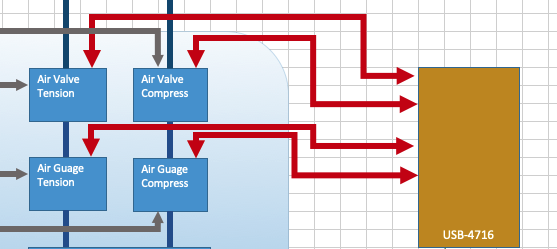
\includegraphics[width=3.12500in]{jira_imgs/3435.png}

}
\hdashrule[0.5ex]{\textwidth}{1pt}{3mm}
  Expected Result \\
{\footnotesize
The air valves and gauges are hooked up to the USB-4716 readout device.~

}
\hdashrule[0.5ex]{\textwidth}{1pt}{3mm}
  Actual Result \\
{\footnotesize

}
\begin{tabular}{p{2cm}p{14cm}}
\toprule
Step 6 & Step Execution Status: \textbf{ Not Executed } \\ \hline
\end{tabular}
 Description \\
{\footnotesize
Make the connection between the MB5U readout electronics and the
renishaw encoders.

}
\hdashrule[0.5ex]{\textwidth}{1pt}{3mm}
  Expected Result \\
{\footnotesize
The MB5U readouts are connected to the encoders.

}
\hdashrule[0.5ex]{\textwidth}{1pt}{3mm}
  Actual Result \\
{\footnotesize

}
\begin{tabular}{p{2cm}p{14cm}}
\toprule
Step 7 & Step Execution Status: \textbf{ Not Executed } \\ \hline
\end{tabular}
 Description \\
{\footnotesize
Make the connection between the 9150 load cell readout electronic and
the load cell.

}
\hdashrule[0.5ex]{\textwidth}{1pt}{3mm}
  Expected Result \\
{\footnotesize
The load cell is connected to the load cell readout electronic.

}
\hdashrule[0.5ex]{\textwidth}{1pt}{3mm}
  Actual Result \\
{\footnotesize

}
\begin{tabular}{p{2cm}p{14cm}}
\toprule
Step 8 & Step Execution Status: \textbf{ Not Executed } \\ \hline
\end{tabular}
 Description \\
{\footnotesize
Make the connection between the Hexapod Actuator to the thermal
scanner.~

}
\hdashrule[0.5ex]{\textwidth}{1pt}{3mm}
  Expected Result \\
{\footnotesize
The thermal scanner is connected to the hexapod actuator.

}
\hdashrule[0.5ex]{\textwidth}{1pt}{3mm}
  Actual Result \\
{\footnotesize

}
\begin{tabular}{p{2cm}p{14cm}}
\toprule
Step 9 & Step Execution Status: \textbf{ Not Executed } \\ \hline
\end{tabular}
 Description \\
{\footnotesize
Connect the following to the USB 3.0 Hub:

\begin{itemize}
\tightlist
\item
  (2) connections for MB5U Readout Electronic
\item
  USB-4716 Readout Device/Labjack T4
\item
  Temperature Readout
\item
  9150 Load Cell Readout Electronic
\end{itemize}

}
\hdashrule[0.5ex]{\textwidth}{1pt}{3mm}
  Expected Result \\
{\footnotesize
The USB 3.0 Hub is now connected to the readout electronics from the
previous steps.~

}
\hdashrule[0.5ex]{\textwidth}{1pt}{3mm}
  Actual Result \\
{\footnotesize

}
\begin{tabular}{p{2cm}p{14cm}}
\toprule
Step 10 & Step Execution Status: \textbf{ Not Executed } \\ \hline
\end{tabular}
 Description \\
{\footnotesize
Connect the laptop with LabVIEW software to the USB 3.0 Hub.

}
\hdashrule[0.5ex]{\textwidth}{1pt}{3mm}
  Expected Result \\
{\footnotesize
The Laptop is connected to the USB 3.0 Hub and to the subsequent readout
electronics.~

}
\hdashrule[0.5ex]{\textwidth}{1pt}{3mm}
  Actual Result \\
{\footnotesize

}
\begin{tabular}{p{2cm}p{14cm}}
\toprule
Step 11 & Step Execution Status: \textbf{ Not Executed } \\ \hline
\end{tabular}
 Description \\
{\footnotesize
Connect the laptop to the Copley Motor drive of the Control Box.

}
\hdashrule[0.5ex]{\textwidth}{1pt}{3mm}
  Expected Result \\
{\footnotesize
The laptop is connected to the control box.

}
\hdashrule[0.5ex]{\textwidth}{1pt}{3mm}
  Actual Result \\
{\footnotesize

}
\begin{tabular}{p{2cm}p{14cm}}
\toprule
Step 12 & Step Execution Status: \textbf{ Not Executed } \\ \hline
\end{tabular}
 Description \\
{\footnotesize
Set up the USB 3.0 Hub close to the test fixture and connect it to a
power source.~

}
\hdashrule[0.5ex]{\textwidth}{1pt}{3mm}
  Expected Result \\
{\footnotesize
The USB 3.0 Hub is connected and all readout devices are powered on.~

}
\hdashrule[0.5ex]{\textwidth}{1pt}{3mm}
  Actual Result \\
{\footnotesize

}
\begin{tabular}{p{2cm}p{14cm}}
\toprule
Step 13 & Step Execution Status: \textbf{ Not Executed } \\ \hline
\end{tabular}
 Description \\
{\footnotesize
Verify that the output data from the readout devices are available on
the laptop.

}
\hdashrule[0.5ex]{\textwidth}{1pt}{3mm}
  Expected Result \\
{\footnotesize
The laptop is seen to be able to communicate with the readout devices.

}
\hdashrule[0.5ex]{\textwidth}{1pt}{3mm}
  Actual Result \\
{\footnotesize

}
\begin{tabular}{p{2cm}p{14cm}}
\toprule
Step 14 & Step Execution Status: \textbf{ Not Executed } \\ \hline
\end{tabular}
 Description \\
{\footnotesize
Open Labview 2021 in the computer used for Test Setup.

}
\hdashrule[0.5ex]{\textwidth}{1pt}{3mm}
  Expected Result \\
{\footnotesize
Labview 2021 opens successfully.

}
\hdashrule[0.5ex]{\textwidth}{1pt}{3mm}
  Actual Result \\
{\footnotesize

}
\begin{tabular}{p{2cm}p{14cm}}
\toprule
Step 15 & Step Execution Status: \textbf{ Not Executed } \\ \hline
\end{tabular}
 Description \\
{\footnotesize
Open the Labview VI files from the project directory including sub VIs-
Tovey Closed loop.vi, Voltage Regulation.vi and Biss Reader.vi

}
\hdashrule[0.5ex]{\textwidth}{1pt}{3mm}
  Expected Result \\
{\footnotesize
Front panel of VI and sub VI files open without any error.

}
\hdashrule[0.5ex]{\textwidth}{1pt}{3mm}
  Actual Result \\
{\footnotesize

}
\begin{tabular}{p{2cm}p{14cm}}
\toprule
Step 16 & Step Execution Status: \textbf{ Not Executed } \\ \hline
\end{tabular}
 Description \\
{\footnotesize
Configure the Biss Reader.vi file with the appropriate configuration
file and following the IBISS operation manual.~

}
\hdashrule[0.5ex]{\textwidth}{1pt}{3mm}
  Expected Result \\
{\footnotesize
\href{https://jira.lsstcorp.org/rest/tests/1.0/attachment/3555}{BiSS\_config.cfg}
is loaded in the LabView configuration (Misc Tab under Load DLL). The
configuration file is based on the IBISS operation manual.

}
\hdashrule[0.5ex]{\textwidth}{1pt}{3mm}
  Actual Result \\
{\footnotesize

}
\begin{tabular}{p{2cm}p{14cm}}
\toprule
Step 17 & Step Execution Status: \textbf{ Not Executed } \\ \hline
\end{tabular}
 Description \\
{\footnotesize
Click Run button on the on the block diagram toolbar of the Labview VI
front panel.

}
\hdashrule[0.5ex]{\textwidth}{1pt}{3mm}
  Expected Result \\
{\footnotesize
LabView VI and ~associated sub Vi runs successfully. Initially all the
graphs and input values will be blank.

}
\hdashrule[0.5ex]{\textwidth}{1pt}{3mm}
  Actual Result \\
{\footnotesize

}
\begin{tabular}{p{2cm}p{14cm}}
\toprule
Step 18 & Step Execution Status: \textbf{ Not Executed } \\ \hline
\end{tabular}
 Description \\
{\footnotesize
Send a command through LabVIEW ~voltage Regulation.vi to set the voltage
on the compression valve only to 3V.

}
\hdashrule[0.5ex]{\textwidth}{1pt}{3mm}
  Expected Result \\
{\footnotesize
The command is accepted, the pneumatic valve shows the applied voltage
only on the compression valve and the applied compression force can be
seen on the LabView front panel Time vs Load graph.~

}
\hdashrule[0.5ex]{\textwidth}{1pt}{3mm}
  Actual Result \\
{\footnotesize

}
\begin{tabular}{p{2cm}p{14cm}}
\toprule
Step 19 & Step Execution Status: \textbf{ Not Executed } \\ \hline
\end{tabular}
 Description \\
{\footnotesize
Send a command through LabVIEW voltage Regulation.vi to reset the
compression valve to 0V.

}
\hdashrule[0.5ex]{\textwidth}{1pt}{3mm}
  Expected Result \\
{\footnotesize
The command is accepted. The applied force can be seen as zero load on
the LabView front panel Time vs Load graph. Load Cell Reader also shows
zero load.

}
\hdashrule[0.5ex]{\textwidth}{1pt}{3mm}
  Actual Result \\
{\footnotesize

}
\begin{tabular}{p{2cm}p{14cm}}
\toprule
Step 20 & Step Execution Status: \textbf{ Not Executed } \\ \hline
\end{tabular}
 Description \\
{\footnotesize
Send a command through LabVIEW to reset the tension valve to 3V.

}
\hdashrule[0.5ex]{\textwidth}{1pt}{3mm}
  Expected Result \\
{\footnotesize
The command is accepted, the readout electronic shows the applied
voltage only on the tension valve and the applied tension force can be
seen on the LabView front panel Time vs Load graph.

}
\hdashrule[0.5ex]{\textwidth}{1pt}{3mm}
  Actual Result \\
{\footnotesize

}
\begin{tabular}{p{2cm}p{14cm}}
\toprule
Step 21 & Step Execution Status: \textbf{ Not Executed } \\ \hline
\end{tabular}
 Description \\
{\footnotesize
Send a command through LabVIEW to reset the tension valve to 0V.

}
\hdashrule[0.5ex]{\textwidth}{1pt}{3mm}
  Expected Result \\
{\footnotesize
The command is accepted, the readout electronic no longer shows the
applied voltage on the tension valve and there is no longer any tension
force on the LabView front panel Time vs Load graph.

}
\hdashrule[0.5ex]{\textwidth}{1pt}{3mm}
  Actual Result \\
{\footnotesize

}
\begin{tabular}{p{2cm}p{14cm}}
\toprule
Step 22 & Step Execution Status: \textbf{ Not Executed } \\ \hline
\end{tabular}
 Description \\
{\footnotesize
Verify the laptop is reading the renishaw scales usinthe Biss Reader.vi
file and determine the zero stroke position.

}
\hdashrule[0.5ex]{\textwidth}{1pt}{3mm}
  Test Data \\
 {\footnotesize
\textbf{Note:~}Moog's original test procedure cited the zero position to
be at 40mm since the full length was 80mm.

}
\hdashrule[0.5ex]{\textwidth}{1pt}{3mm}
  Expected Result \\
{\footnotesize
40mm encoder readings shown in Labview front panel of the .vi file.~\\
The zero stroke position has been determined and can be used as a
reference for the offset of future moves.

}
\hdashrule[0.5ex]{\textwidth}{1pt}{3mm}
  Actual Result \\
{\footnotesize

}

\paragraph{ LVV-T2428 - Hexapod - Actuator Stiffness Test }\mbox{}\\

Version \textbf{1}.
Status \textbf{Approved}.
Open  \href{https://jira.lsstcorp.org/secure/Tests.jspa#/testCase/LVV-T2428}{\textit{ LVV-T2428 } }
test case in Jira.



\textbf{ Preconditions}:\\


Execution status: {\bf Not Executed }

Final comment:\\


Detailed steps results:

\begin{tabular}{p{2cm}p{14cm}}
\toprule
Step 1.1 & Step Execution Status: \textbf{ Not Executed } \\ \hline
\end{tabular}
 Description \\
{\footnotesize
Open Labview 2021 in the computer used for Test Setup.

}
\hdashrule[0.5ex]{\textwidth}{1pt}{3mm}
  Test Data \\
 {\footnotesize
\textbf{Note:~}The first three steps are conditional because these steps
are included as part of the Test Setup procedure and may not be
necessary if LabView is still open.

}
\hdashrule[0.5ex]{\textwidth}{1pt}{3mm}
  Expected Result \\
{\footnotesize
Labview 2021 opens successfully.

}
\hdashrule[0.5ex]{\textwidth}{1pt}{3mm}
  Actual Result \\
{\footnotesize

}
\begin{tabular}{p{2cm}p{14cm}}
\toprule
Step 1.2 & Step Execution Status: \textbf{ Not Executed } \\ \hline
\end{tabular}
 Description \\
{\footnotesize
Open the Labview VI files from the project directory including sub VIs-
Tovey Closed loop.vi, Voltage Regulation.vi and Biss Reader.vi

}
\hdashrule[0.5ex]{\textwidth}{1pt}{3mm}
  Expected Result \\
{\footnotesize
Front panel of VI and sub VI files open without any error.

}
\hdashrule[0.5ex]{\textwidth}{1pt}{3mm}
  Actual Result \\
{\footnotesize

}
\begin{tabular}{p{2cm}p{14cm}}
\toprule
Step 1.3 & Step Execution Status: \textbf{ Not Executed } \\ \hline
\end{tabular}
 Description \\
{\footnotesize
Click Run button on the on the block diagram toolbar of the Labview VI
front panel.

}
\hdashrule[0.5ex]{\textwidth}{1pt}{3mm}
  Expected Result \\
{\footnotesize
LabView VI and ~associated sub Vi runs successfully. Initially all the
graphs and input values will be blank.

}
\hdashrule[0.5ex]{\textwidth}{1pt}{3mm}
  Actual Result \\
{\footnotesize

}
\begin{tabular}{p{2cm}p{14cm}}
\toprule
Step 1.4 & Step Execution Status: \textbf{ Not Executed } \\ \hline
\end{tabular}
 Description \\
{\footnotesize
Position the actuator at its center of stroke.

}
\hdashrule[0.5ex]{\textwidth}{1pt}{3mm}
  Test Data \\
 {\footnotesize
\textbf{Note:~}The original zero position/center of stroke position was
determined to be a linear encoder reading of 40mm. For the purpose of
this test, the same center of stroke position will be used.

}
\hdashrule[0.5ex]{\textwidth}{1pt}{3mm}
  Expected Result \\
{\footnotesize
Actuator positioned at its center of stroke position ~confirmed by
encoder reading in the LabView.\\[2\baselineskip]

}
\hdashrule[0.5ex]{\textwidth}{1pt}{3mm}
  Actual Result \\
{\footnotesize

}
\begin{tabular}{p{2cm}p{14cm}}
\toprule
Step 1.5 & Step Execution Status: \textbf{ Not Executed } \\ \hline
\end{tabular}
 Description \\
{\footnotesize
Disable Motor Power by pressing the Emergency stop button on the control
box.

}
\hdashrule[0.5ex]{\textwidth}{1pt}{3mm}
  Expected Result \\
{\footnotesize
Motor power disabled.

}
\hdashrule[0.5ex]{\textwidth}{1pt}{3mm}
  Actual Result \\
{\footnotesize

}
\begin{tabular}{p{2cm}p{14cm}}
\toprule
Step 1.6 & Step Execution Status: \textbf{ Not Executed } \\ \hline
\end{tabular}
 Description \\
{\footnotesize
Iteration {1}⁠ : Increase the load on the actuator from 0 kN to
approximately 30kN (6744 lbf) tension

}
\hdashrule[0.5ex]{\textwidth}{1pt}{3mm}
  Test Data \\
 {\footnotesize
\textbf{Note:~}In order to apply a tension force of 30 KN:

\begin{itemize}
\tightlist
\item
  Set pneumatic valve (closest to hexapod actuator side) to 3.5V (0-10
  Vdc) while the other valve remains at 0V.
\item
  increase air supply using LabVIEW function~
\end{itemize}

}
\hdashrule[0.5ex]{\textwidth}{1pt}{3mm}
  Expected Result \\
{\footnotesize
Load cell reader shows the applied 30 KN tension force.\\
LabView displays the voltage being applied.

}
\hdashrule[0.5ex]{\textwidth}{1pt}{3mm}
  Actual Result \\
{\footnotesize

}
\begin{tabular}{p{2cm}p{14cm}}
\toprule
Step 1.7 & Step Execution Status: \textbf{ Not Executed } \\ \hline
\end{tabular}
 Description \\
{\footnotesize
Iteration {{1}⁠} :Reduce the load through zero load to approximately 30
kN (6744 lbf) compression, and return to zero load.

}
\hdashrule[0.5ex]{\textwidth}{1pt}{3mm}
  Test Data \\
 {\footnotesize
\textbf{Note:~}In order to apply a compression force of 30kN:\\

\begin{itemize}
\tightlist
\item
  Set pneumatic valve (far from the hexapod actuator side) to 3.5V (0-10
  Vdc) while the other valve remains at 0V ( reverse from step 6).
\item
  increase air supply using LabVIEW function~
\end{itemize}

}
\hdashrule[0.5ex]{\textwidth}{1pt}{3mm}
  Expected Result \\
{\footnotesize
Load graphs shows the fluctuation of loads from 30 KN tension to zero to
30 KN compression and back to zero load in LabView.~

}
\hdashrule[0.5ex]{\textwidth}{1pt}{3mm}
  Actual Result \\
{\footnotesize

}
\begin{tabular}{p{2cm}p{14cm}}
\toprule
Step 1.8 & Step Execution Status: \textbf{ Not Executed } \\ \hline
\end{tabular}
 Description \\
{\footnotesize
Record the actual displacement as measured by the two external encoders
as LabView graph ( Time vs Displacement).\\[2\baselineskip]

}
\hdashrule[0.5ex]{\textwidth}{1pt}{3mm}
  Expected Result \\
{\footnotesize
Actual displacement measured by the average of the two external encoders
~recorded in the LabView graph.

}
\hdashrule[0.5ex]{\textwidth}{1pt}{3mm}
  Actual Result \\
{\footnotesize

}
\begin{tabular}{p{2cm}p{14cm}}
\toprule
Step 1.9 & Step Execution Status: \textbf{ Not Executed } \\ \hline
\end{tabular}
 Description \\
{\footnotesize
View the a force vs displacement plot in the Labview.~\\[2\baselineskip]

}
\hdashrule[0.5ex]{\textwidth}{1pt}{3mm}
  Expected Result \\
{\footnotesize
The expected actuator stiffness is \textgreater{}= 134 N/um at center
stroke.~\\[2\baselineskip]

}
\hdashrule[0.5ex]{\textwidth}{1pt}{3mm}
  Actual Result \\
{\footnotesize

}
\begin{tabular}{p{2cm}p{14cm}}
\toprule
Step 2.0 & Step Execution Status: \textbf{ Not Executed } \\ \hline
\end{tabular}
 Description \\
{\footnotesize
Check if all the test results are recorded in excel spreadsheets.

}
\hdashrule[0.5ex]{\textwidth}{1pt}{3mm}
  Expected Result \\
{\footnotesize
Test Results are recorded in the excel spreadsheets residing in the
LabView Folder directory.

}
\hdashrule[0.5ex]{\textwidth}{1pt}{3mm}
  Actual Result \\
{\footnotesize

}
\begin{tabular}{p{2cm}p{14cm}}
\toprule
Step 2.1 & Step Execution Status: \textbf{ Not Executed } \\ \hline
\end{tabular}
 Description \\
{\footnotesize
Close all the Labview VI files.

}
\hdashrule[0.5ex]{\textwidth}{1pt}{3mm}
  Test Data \\
 {\footnotesize
\textbf{Note:~}Labview can be left open in order to continue to the next
test. However, it may be necessary to reset the application before
starting the next test.

}
\hdashrule[0.5ex]{\textwidth}{1pt}{3mm}
  Expected Result \\
{\footnotesize
All the VI files are closed and Labview 2021 application window closes.

}
\hdashrule[0.5ex]{\textwidth}{1pt}{3mm}
  Actual Result \\
{\footnotesize

}
\begin{tabular}{p{2cm}p{14cm}}
\toprule
Step 2.1 & Step Execution Status: \textbf{ Not Executed } \\ \hline
\end{tabular}
 Description \\
{\footnotesize
Open Labview 2021 in the computer used for Test Setup.

}
\hdashrule[0.5ex]{\textwidth}{1pt}{3mm}
  Test Data \\
 {\footnotesize
\textbf{Note:~}The first three steps are conditional because these steps
are included as part of the Test Setup procedure and may not be
necessary if LabView is still open.

}
\hdashrule[0.5ex]{\textwidth}{1pt}{3mm}
  Expected Result \\
{\footnotesize
Labview 2021 opens successfully.

}
\hdashrule[0.5ex]{\textwidth}{1pt}{3mm}
  Actual Result \\
{\footnotesize

}
\begin{tabular}{p{2cm}p{14cm}}
\toprule
Step 2.2 & Step Execution Status: \textbf{ Not Executed } \\ \hline
\end{tabular}
 Description \\
{\footnotesize
Open the Labview VI files from the project directory including sub VIs-
Tovey Closed loop.vi, Voltage Regulation.vi and Biss Reader.vi

}
\hdashrule[0.5ex]{\textwidth}{1pt}{3mm}
  Expected Result \\
{\footnotesize
Front panel of VI and sub VI files open without any error.

}
\hdashrule[0.5ex]{\textwidth}{1pt}{3mm}
  Actual Result \\
{\footnotesize

}
\begin{tabular}{p{2cm}p{14cm}}
\toprule
Step 2.3 & Step Execution Status: \textbf{ Not Executed } \\ \hline
\end{tabular}
 Description \\
{\footnotesize
Click Run button on the on the block diagram toolbar of the Labview VI
front panel.

}
\hdashrule[0.5ex]{\textwidth}{1pt}{3mm}
  Expected Result \\
{\footnotesize
LabView VI and ~associated sub Vi runs successfully. Initially all the
graphs and input values will be blank.

}
\hdashrule[0.5ex]{\textwidth}{1pt}{3mm}
  Actual Result \\
{\footnotesize

}
\begin{tabular}{p{2cm}p{14cm}}
\toprule
Step 2.4 & Step Execution Status: \textbf{ Not Executed } \\ \hline
\end{tabular}
 Description \\
{\footnotesize
Position the actuator at its center of stroke.

}
\hdashrule[0.5ex]{\textwidth}{1pt}{3mm}
  Test Data \\
 {\footnotesize
\textbf{Note:~}The original zero position/center of stroke position was
determined to be a linear encoder reading of 40mm. For the purpose of
this test, the same center of stroke position will be used.

}
\hdashrule[0.5ex]{\textwidth}{1pt}{3mm}
  Expected Result \\
{\footnotesize
Actuator positioned at its center of stroke position ~confirmed by
encoder reading in the LabView.\\[2\baselineskip]

}
\hdashrule[0.5ex]{\textwidth}{1pt}{3mm}
  Actual Result \\
{\footnotesize

}
\begin{tabular}{p{2cm}p{14cm}}
\toprule
Step 2.5 & Step Execution Status: \textbf{ Not Executed } \\ \hline
\end{tabular}
 Description \\
{\footnotesize
Disable Motor Power by pressing the Emergency stop button on the control
box.

}
\hdashrule[0.5ex]{\textwidth}{1pt}{3mm}
  Expected Result \\
{\footnotesize
Motor power disabled.

}
\hdashrule[0.5ex]{\textwidth}{1pt}{3mm}
  Actual Result \\
{\footnotesize

}
\begin{tabular}{p{2cm}p{14cm}}
\toprule
Step 2.6 & Step Execution Status: \textbf{ Not Executed } \\ \hline
\end{tabular}
 Description \\
{\footnotesize
Iteration {2}⁠ : Increase the load on the actuator from 0 kN to
approximately 30kN (6744 lbf) tension

}
\hdashrule[0.5ex]{\textwidth}{1pt}{3mm}
  Test Data \\
 {\footnotesize
\textbf{Note:~}In order to apply a tension force of 30 KN:

\begin{itemize}
\tightlist
\item
  Set pneumatic valve (closest to hexapod actuator side) to 3.5V (0-10
  Vdc) while the other valve remains at 0V.
\item
  increase air supply using LabVIEW function~
\end{itemize}

}
\hdashrule[0.5ex]{\textwidth}{1pt}{3mm}
  Expected Result \\
{\footnotesize
Load cell reader shows the applied 30 KN tension force.\\
LabView displays the voltage being applied.

}
\hdashrule[0.5ex]{\textwidth}{1pt}{3mm}
  Actual Result \\
{\footnotesize

}
\begin{tabular}{p{2cm}p{14cm}}
\toprule
Step 2.7 & Step Execution Status: \textbf{ Not Executed } \\ \hline
\end{tabular}
 Description \\
{\footnotesize
Iteration {{2}⁠} :Reduce the load through zero load to approximately 30
kN (6744 lbf) compression, and return to zero load.

}
\hdashrule[0.5ex]{\textwidth}{1pt}{3mm}
  Test Data \\
 {\footnotesize
\textbf{Note:~}In order to apply a compression force of 30kN:\\

\begin{itemize}
\tightlist
\item
  Set pneumatic valve (far from the hexapod actuator side) to 3.5V (0-10
  Vdc) while the other valve remains at 0V ( reverse from step 6).
\item
  increase air supply using LabVIEW function~
\end{itemize}

}
\hdashrule[0.5ex]{\textwidth}{1pt}{3mm}
  Expected Result \\
{\footnotesize
Load graphs shows the fluctuation of loads from 30 KN tension to zero to
30 KN compression and back to zero load in LabView.~

}
\hdashrule[0.5ex]{\textwidth}{1pt}{3mm}
  Actual Result \\
{\footnotesize

}
\begin{tabular}{p{2cm}p{14cm}}
\toprule
Step 2.8 & Step Execution Status: \textbf{ Not Executed } \\ \hline
\end{tabular}
 Description \\
{\footnotesize
Record the actual displacement as measured by the two external encoders
as LabView graph ( Time vs Displacement).\\[2\baselineskip]

}
\hdashrule[0.5ex]{\textwidth}{1pt}{3mm}
  Expected Result \\
{\footnotesize
Actual displacement measured by the average of the two external encoders
~recorded in the LabView graph.

}
\hdashrule[0.5ex]{\textwidth}{1pt}{3mm}
  Actual Result \\
{\footnotesize

}
\begin{tabular}{p{2cm}p{14cm}}
\toprule
Step 2.9 & Step Execution Status: \textbf{ Not Executed } \\ \hline
\end{tabular}
 Description \\
{\footnotesize
View the a force vs displacement plot in the Labview.~\\[2\baselineskip]

}
\hdashrule[0.5ex]{\textwidth}{1pt}{3mm}
  Expected Result \\
{\footnotesize
The expected actuator stiffness is \textgreater{}= 134 N/um at center
stroke.~\\[2\baselineskip]

}
\hdashrule[0.5ex]{\textwidth}{1pt}{3mm}
  Actual Result \\
{\footnotesize

}
\begin{tabular}{p{2cm}p{14cm}}
\toprule
Step 3.0 & Step Execution Status: \textbf{ Not Executed } \\ \hline
\end{tabular}
 Description \\
{\footnotesize
Check if all the test results are recorded in excel spreadsheets.

}
\hdashrule[0.5ex]{\textwidth}{1pt}{3mm}
  Expected Result \\
{\footnotesize
Test Results are recorded in the excel spreadsheets residing in the
LabView Folder directory.

}
\hdashrule[0.5ex]{\textwidth}{1pt}{3mm}
  Actual Result \\
{\footnotesize

}
\begin{tabular}{p{2cm}p{14cm}}
\toprule
Step 3.1 & Step Execution Status: \textbf{ Not Executed } \\ \hline
\end{tabular}
 Description \\
{\footnotesize
Close all the Labview VI files.

}
\hdashrule[0.5ex]{\textwidth}{1pt}{3mm}
  Test Data \\
 {\footnotesize
\textbf{Note:~}Labview can be left open in order to continue to the next
test. However, it may be necessary to reset the application before
starting the next test.

}
\hdashrule[0.5ex]{\textwidth}{1pt}{3mm}
  Expected Result \\
{\footnotesize
All the VI files are closed and Labview 2021 application window closes.

}
\hdashrule[0.5ex]{\textwidth}{1pt}{3mm}
  Actual Result \\
{\footnotesize

}

\paragraph{ LVV-T2432 - Hexapod - Actuator Range of Motion Test }\mbox{}\\

Version \textbf{1}.
Status \textbf{Approved}.
Open  \href{https://jira.lsstcorp.org/secure/Tests.jspa#/testCase/LVV-T2432}{\textit{ LVV-T2432 } }
test case in Jira.

To verify that the range of motions for the actuators stay within the
determined limits.

\textbf{ Preconditions}:\\
The range limits should be determined to achieve the camera hexapod's
simultaneous range of motion requirements.

Execution status: {\bf Not Executed }

Final comment:\\


Detailed steps results:

\begin{tabular}{p{2cm}p{14cm}}
\toprule
Step 1 & Step Execution Status: \textbf{ Not Executed } \\ \hline
\end{tabular}
 Description \\
{\footnotesize
Open Labview 2021 in the computer used for Test Setup.

}
\hdashrule[0.5ex]{\textwidth}{1pt}{3mm}
  Test Data \\
 {\footnotesize
The first three steps are conditional because these steps are included
as part of the Test Setup procedure and may not be necessary if LabView
is still open.\\[3\baselineskip]

}
\hdashrule[0.5ex]{\textwidth}{1pt}{3mm}
  Expected Result \\
{\footnotesize
Labview 2021 opens successfully.

}
\hdashrule[0.5ex]{\textwidth}{1pt}{3mm}
  Actual Result \\
{\footnotesize

}
\begin{tabular}{p{2cm}p{14cm}}
\toprule
Step 2 & Step Execution Status: \textbf{ Not Executed } \\ \hline
\end{tabular}
 Description \\
{\footnotesize
Open the Labview Biss Reader.vi file.~

}
\hdashrule[0.5ex]{\textwidth}{1pt}{3mm}
  Expected Result \\
{\footnotesize
Front panel of the VI a file open without any error.

}
\hdashrule[0.5ex]{\textwidth}{1pt}{3mm}
  Actual Result \\
{\footnotesize

}
\begin{tabular}{p{2cm}p{14cm}}
\toprule
Step 3 & Step Execution Status: \textbf{ Not Executed } \\ \hline
\end{tabular}
 Description \\
{\footnotesize
Click Run button on the on the block diagram toolbar of the Labview VI
front panel.

}
\hdashrule[0.5ex]{\textwidth}{1pt}{3mm}
  Expected Result \\
{\footnotesize
Biss Reader.vi run successfully. Initially all the graphs and input
values will be blank.

}
\hdashrule[0.5ex]{\textwidth}{1pt}{3mm}
  Actual Result \\
{\footnotesize

}
\begin{tabular}{p{2cm}p{14cm}}
\toprule
Step 4 & Step Execution Status: \textbf{ Not Executed } \\ \hline
\end{tabular}
 Description \\
{\footnotesize
Set software actuator stroke limits using the copley software to +/-
14.00mm.

}
\hdashrule[0.5ex]{\textwidth}{1pt}{3mm}
  Expected Result \\
{\footnotesize
Software actuator stroke limits set to +/- 14.00mm.

}
\hdashrule[0.5ex]{\textwidth}{1pt}{3mm}
  Actual Result \\
{\footnotesize

}
\begin{tabular}{p{2cm}p{14cm}}
\toprule
Step 5 & Step Execution Status: \textbf{ Not Executed } \\ \hline
\end{tabular}
 Description \\
{\footnotesize
Move the actuator forward and backward to confirm that positive position
commands correspond to extensions of the actuator and negative position
commands correspond to retractions of the actuator. If not, flipped the
sign of the encoder readings in software.~\\[2\baselineskip]

}
\hdashrule[0.5ex]{\textwidth}{1pt}{3mm}
  Expected Result \\
{\footnotesize
Positive position commands correspond to extensions; Negative position
commands correspond to retractions of the actuator.~

}
\hdashrule[0.5ex]{\textwidth}{1pt}{3mm}
  Actual Result \\
{\footnotesize

}
\begin{tabular}{p{2cm}p{14cm}}
\toprule
Step 6 & Step Execution Status: \textbf{ Not Executed } \\ \hline
\end{tabular}
 Description \\
{\footnotesize
Set the motor drive to halt motion using the control box and copley
software if a limit switch is tripped.\\[3\baselineskip]

}
\hdashrule[0.5ex]{\textwidth}{1pt}{3mm}
  Expected Result \\
{\footnotesize
Motor drive set to halt position if a limit switch is tripped.~

}
\hdashrule[0.5ex]{\textwidth}{1pt}{3mm}
  Actual Result \\
{\footnotesize

}
\begin{tabular}{p{2cm}p{14cm}}
\toprule
Step 7 & Step Execution Status: \textbf{ Not Executed } \\ \hline
\end{tabular}
 Description \\
{\footnotesize
Extend the actuator to its position stroke limit of +14mm using the
copley software and the~ control box.

}
\hdashrule[0.5ex]{\textwidth}{1pt}{3mm}
  Expected Result \\
{\footnotesize
Actuator extended to its position stroke limit of +14mm.

}
\hdashrule[0.5ex]{\textwidth}{1pt}{3mm}
  Actual Result \\
{\footnotesize

}
\begin{tabular}{p{2cm}p{14cm}}
\toprule
Step 8 & Step Execution Status: \textbf{ Not Executed } \\ \hline
\end{tabular}
 Description \\
{\footnotesize
Ensure that the actuator reaches this position without hitting the
mechanical end stop or extension limit switch.

}
\hdashrule[0.5ex]{\textwidth}{1pt}{3mm}
  Expected Result \\
{\footnotesize
Encoder reading in LabView shows that actuator reached the position.~\\
Mechanical End Stop/Extension Limit switch not hit.

}
\hdashrule[0.5ex]{\textwidth}{1pt}{3mm}
  Actual Result \\
{\footnotesize

}
\begin{tabular}{p{2cm}p{14cm}}
\toprule
Step 9 & Step Execution Status: \textbf{ Not Executed } \\ \hline
\end{tabular}
 Description \\
{\footnotesize
If the extension limit switch is contacted, the extension limit switch
position will need to be adjusted to be greater than 14mm and then the
try to extend the actuator to the position stroke limit of +14mm using
copley software and the control box.

}
\hdashrule[0.5ex]{\textwidth}{1pt}{3mm}
  Expected Result \\
{\footnotesize
Extension Limit Switch position readjusted and extended to the position
stroke limit of +14mm.

}
\hdashrule[0.5ex]{\textwidth}{1pt}{3mm}
  Actual Result \\
{\footnotesize

}
\begin{tabular}{p{2cm}p{14cm}}
\toprule
Step 10 & Step Execution Status: \textbf{ Not Executed } \\ \hline
\end{tabular}
 Description \\
{\footnotesize
Ensure that the actuator reaches this position without hitting the
mechanical end stop or extension limit switch.

}
\hdashrule[0.5ex]{\textwidth}{1pt}{3mm}
  Expected Result \\
{\footnotesize
Encoder reading in LabView shows that actuator reached the position.\\
Mechanical End Stop/Extension Limit switch not hit.

}
\hdashrule[0.5ex]{\textwidth}{1pt}{3mm}
  Actual Result \\
{\footnotesize

}
\begin{tabular}{p{2cm}p{14cm}}
\toprule
Step 11 & Step Execution Status: \textbf{ Not Executed } \\ \hline
\end{tabular}
 Description \\
{\footnotesize
Move the extension actuator stroke limit using the copley software to
+15.00mm .

}
\hdashrule[0.5ex]{\textwidth}{1pt}{3mm}
  Expected Result \\
{\footnotesize
Extension actuator stroke limit moved to +15.00mm.~

}
\hdashrule[0.5ex]{\textwidth}{1pt}{3mm}
  Actual Result \\
{\footnotesize

}
\begin{tabular}{p{2cm}p{14cm}}
\toprule
Step 12 & Step Execution Status: \textbf{ Not Executed } \\ \hline
\end{tabular}
 Description \\
{\footnotesize
Extend the actuator at maximum velocity until the extension limit switch
is actuated.

}
\hdashrule[0.5ex]{\textwidth}{1pt}{3mm}
  Test Data \\
 {\footnotesize
\textbf{Note:~}The maximum velocity is +/-0.5mm/s

}
\hdashrule[0.5ex]{\textwidth}{1pt}{3mm}
  Expected Result \\
{\footnotesize
Actuator extended at maximum velocity until the extension limit switch
is actuated.~

}
\hdashrule[0.5ex]{\textwidth}{1pt}{3mm}
  Actual Result \\
{\footnotesize

}
\begin{tabular}{p{2cm}p{14cm}}
\toprule
Step 13 & Step Execution Status: \textbf{ Not Executed } \\ \hline
\end{tabular}
 Description \\
{\footnotesize
If the actuator hits the stroke limit before tripping the limit switch
or appears to contact the end stop after tripping the limit switch
(before it can stop), reposition the limit switch. Then, repeat test
using copley software and the control box.\\[2\baselineskip]

}
\hdashrule[0.5ex]{\textwidth}{1pt}{3mm}
  Expected Result \\
{\footnotesize
Limit switch repositioned and extended the actuator to the position
stroke limit of +15mm.~

}
\hdashrule[0.5ex]{\textwidth}{1pt}{3mm}
  Actual Result \\
{\footnotesize

}
\begin{tabular}{p{2cm}p{14cm}}
\toprule
Step 14 & Step Execution Status: \textbf{ Not Executed } \\ \hline
\end{tabular}
 Description \\
{\footnotesize
Record the final position of the limit switch.~\\[2\baselineskip]

}
\hdashrule[0.5ex]{\textwidth}{1pt}{3mm}
  Expected Result \\
{\footnotesize
\textbf{Final position of the limit switch around +14.50mm.}

}
\hdashrule[0.5ex]{\textwidth}{1pt}{3mm}
  Actual Result \\
{\footnotesize

}
\begin{tabular}{p{2cm}p{14cm}}
\toprule
Step 15 & Step Execution Status: \textbf{ Not Executed } \\ \hline
\end{tabular}
 Description \\
{\footnotesize
Repeat the steps 6-14 two more times to assess limit switch position
repeatability. ~\\[3\baselineskip]

}
\hdashrule[0.5ex]{\textwidth}{1pt}{3mm}
  Expected Result \\
{\footnotesize
Final positions of the limit switch close to step 14 result(Around
+14.50).

}
\hdashrule[0.5ex]{\textwidth}{1pt}{3mm}
  Actual Result \\
{\footnotesize

}
\begin{tabular}{p{2cm}p{14cm}}
\toprule
Step 16 & Step Execution Status: \textbf{ Not Executed } \\ \hline
\end{tabular}
 Description \\
{\footnotesize
Retract the actuator to its position stroke limit of -14 mm using the
copley software and the ~control box.\\[2\baselineskip]

}
\hdashrule[0.5ex]{\textwidth}{1pt}{3mm}
  Expected Result \\
{\footnotesize
Actuator retracted to its position stroke limit of -14.04mm.

}
\hdashrule[0.5ex]{\textwidth}{1pt}{3mm}
  Actual Result \\
{\footnotesize

}
\begin{tabular}{p{2cm}p{14cm}}
\toprule
Step 17 & Step Execution Status: \textbf{ Not Executed } \\ \hline
\end{tabular}
 Description \\
{\footnotesize
Ensure that the actuator reaches this position without hitting the
mechanical end stop or retraction limit switch.

}
\hdashrule[0.5ex]{\textwidth}{1pt}{3mm}
  Expected Result \\
{\footnotesize
Encoder reading in LabView shows that actuator reached the position.\\
Mechanical End Stop/Retraction Limit switch not hit.

}
\hdashrule[0.5ex]{\textwidth}{1pt}{3mm}
  Actual Result \\
{\footnotesize

}
\begin{tabular}{p{2cm}p{14cm}}
\toprule
Step 18 & Step Execution Status: \textbf{ Not Executed } \\ \hline
\end{tabular}
 Description \\
{\footnotesize
If the retraction limit switch is contacted, the retraction limit switch
position will need to be adjusted to be greater than -14mm and then the
try to retract the actuator to the position stroke limit of -14mm using
copley software and the control box.

}
\hdashrule[0.5ex]{\textwidth}{1pt}{3mm}
  Expected Result \\
{\footnotesize
Retraction limit switch position readjusted and the actuator retracted
to the position stroke limit of -14mm.

}
\hdashrule[0.5ex]{\textwidth}{1pt}{3mm}
  Actual Result \\
{\footnotesize

}
\begin{tabular}{p{2cm}p{14cm}}
\toprule
Step 19 & Step Execution Status: \textbf{ Not Executed } \\ \hline
\end{tabular}
 Description \\
{\footnotesize
Ensure that the actuator reaches this position without hitting the
mechanical end stop or retraction limit switch.

}
\hdashrule[0.5ex]{\textwidth}{1pt}{3mm}
  Expected Result \\
{\footnotesize
Encoder reading in LabView shows that actuator reached the position.\\
Mechanical End Stop/Retraction Limit switch not hit.

}
\hdashrule[0.5ex]{\textwidth}{1pt}{3mm}
  Actual Result \\
{\footnotesize

}
\begin{tabular}{p{2cm}p{14cm}}
\toprule
Step 20 & Step Execution Status: \textbf{ Not Executed } \\ \hline
\end{tabular}
 Description \\
{\footnotesize
Move the retraction actuator stroke limit to -15.00mm .~

}
\hdashrule[0.5ex]{\textwidth}{1pt}{3mm}
  Expected Result \\
{\footnotesize
Retraction actuator stroke limit moved to -15.00mm.

}
\hdashrule[0.5ex]{\textwidth}{1pt}{3mm}
  Actual Result \\
{\footnotesize

}
\begin{tabular}{p{2cm}p{14cm}}
\toprule
Step 21 & Step Execution Status: \textbf{ Not Executed } \\ \hline
\end{tabular}
 Description \\
{\footnotesize
Retract the actuator at maximum velocity until the retraction limit
switch is actuated.

}
\hdashrule[0.5ex]{\textwidth}{1pt}{3mm}
  Test Data \\
 {\footnotesize
\textbf{Note:~}The maximum velocity is +/-0.5mm/s

}
\hdashrule[0.5ex]{\textwidth}{1pt}{3mm}
  Expected Result \\
{\footnotesize
Actuator retracted at maximum velocity until the retraction limit switch
is actuated.

}
\hdashrule[0.5ex]{\textwidth}{1pt}{3mm}
  Actual Result \\
{\footnotesize

}
\begin{tabular}{p{2cm}p{14cm}}
\toprule
Step 22 & Step Execution Status: \textbf{ Not Executed } \\ \hline
\end{tabular}
 Description \\
{\footnotesize
If the actuator hits the stroke limit before tripping the limit switch
or appears to contact the end stop after tripping the limit switch
(before it can stop), reposition the limit switch and repeat test.

}
\hdashrule[0.5ex]{\textwidth}{1pt}{3mm}
  Expected Result \\
{\footnotesize
Limit switch repositioned and retracted the actuator to the position
stroke limit of -15mm.

}
\hdashrule[0.5ex]{\textwidth}{1pt}{3mm}
  Actual Result \\
{\footnotesize

}
\begin{tabular}{p{2cm}p{14cm}}
\toprule
Step 23 & Step Execution Status: \textbf{ Not Executed } \\ \hline
\end{tabular}
 Description \\
{\footnotesize
Record the final position of the limit switch.

}
\hdashrule[0.5ex]{\textwidth}{1pt}{3mm}
  Expected Result \\
{\footnotesize
\textbf{Final position of the limit switch around -14.50mm.}

}
\hdashrule[0.5ex]{\textwidth}{1pt}{3mm}
  Actual Result \\
{\footnotesize

}
\begin{tabular}{p{2cm}p{14cm}}
\toprule
Step 24 & Step Execution Status: \textbf{ Not Executed } \\ \hline
\end{tabular}
 Description \\
{\footnotesize
Repeat the steps 16-23 two more times to assess limit switch position
repeatability.

}
\hdashrule[0.5ex]{\textwidth}{1pt}{3mm}
  Expected Result \\
{\footnotesize
Final positions of the limit switch close to step 15 result(Around
-14.50).

}
\hdashrule[0.5ex]{\textwidth}{1pt}{3mm}
  Actual Result \\
{\footnotesize

}
\begin{tabular}{p{2cm}p{14cm}}
\toprule
Step 25 & Step Execution Status: \textbf{ Not Executed } \\ \hline
\end{tabular}
 Description \\
{\footnotesize
Check if all the test results are recorded in excel spreadsheets.

}
\hdashrule[0.5ex]{\textwidth}{1pt}{3mm}
  Expected Result \\
{\footnotesize
Test Results are recorded in the excel spreadsheets residing in the
LabView Folder directory.\\[2\baselineskip]

}
\hdashrule[0.5ex]{\textwidth}{1pt}{3mm}
  Actual Result \\
{\footnotesize

}
\begin{tabular}{p{2cm}p{14cm}}
\toprule
Step 26 & Step Execution Status: \textbf{ Not Executed } \\ \hline
\end{tabular}
 Description \\
{\footnotesize
Close the Labview Vi file.

}
\hdashrule[0.5ex]{\textwidth}{1pt}{3mm}
  Test Data \\
 {\footnotesize
\textbf{Note:~}Labview can be left open in order to continue to the next
test. However, it may be necessary to reset the application before
starting the next test.

}
\hdashrule[0.5ex]{\textwidth}{1pt}{3mm}
  Expected Result \\
{\footnotesize
Labview 2021 application window closes.

}
\hdashrule[0.5ex]{\textwidth}{1pt}{3mm}
  Actual Result \\
{\footnotesize

}

\paragraph{ LVV-T2437 - Hexapod - Actuator Movement Test }\mbox{}\\

Version \textbf{1}.
Status \textbf{Approved}.
Open  \href{https://jira.lsstcorp.org/secure/Tests.jspa#/testCase/LVV-T2437}{\textit{ LVV-T2437 } }
test case in Jira.

The purpose of this test will be to verify that the actuators are able
to move within their velocity and acceleration limits. Furthermore,
during the moves, we will also be verifying that the actuators do not
take more than 2 seconds to settle into place.~

\textbf{ Preconditions}:\\


Execution status: {\bf Not Executed }

Final comment:\\


Detailed steps results:

\begin{tabular}{p{2cm}p{14cm}}
\toprule
Step 1 & Step Execution Status: \textbf{ Not Executed } \\ \hline
\end{tabular}
 Description \\
{\footnotesize
Open Labview 2021 in the computer used for Test Setup.

}
\hdashrule[0.5ex]{\textwidth}{1pt}{3mm}
  Test Data \\
 {\footnotesize
The first three steps are conditional because these steps are included
as part of the Test Setup procedure and may not be necessary if LabView
is still open.

}
\hdashrule[0.5ex]{\textwidth}{1pt}{3mm}
  Expected Result \\
{\footnotesize
Labview 2021 opens successfully.

}
\hdashrule[0.5ex]{\textwidth}{1pt}{3mm}
  Actual Result \\
{\footnotesize

}
\begin{tabular}{p{2cm}p{14cm}}
\toprule
Step 2 & Step Execution Status: \textbf{ Not Executed } \\ \hline
\end{tabular}
 Description \\
{\footnotesize
Open the Labview VI files from the project directory including sub VIs-
Tovey Closed loop.vi, Voltage Regulation.vi and Biss Reader.vi

}
\hdashrule[0.5ex]{\textwidth}{1pt}{3mm}
  Expected Result \\
{\footnotesize
Front panel of VI and sub VI files open without any error.

}
\hdashrule[0.5ex]{\textwidth}{1pt}{3mm}
  Actual Result \\
{\footnotesize

}
\begin{tabular}{p{2cm}p{14cm}}
\toprule
Step 3 & Step Execution Status: \textbf{ Not Executed } \\ \hline
\end{tabular}
 Description \\
{\footnotesize
Click Run button on the on the block diagram toolbar of the Labview VI
front panel.

}
\hdashrule[0.5ex]{\textwidth}{1pt}{3mm}
  Expected Result \\
{\footnotesize
LabView VI and ~associated sub Vi runs successfully. Initially all the
graphs and input values will be blank.

}
\hdashrule[0.5ex]{\textwidth}{1pt}{3mm}
  Actual Result \\
{\footnotesize

}
\begin{tabular}{p{2cm}p{14cm}}
\toprule
Step 4 & Step Execution Status: \textbf{ Not Executed } \\ \hline
\end{tabular}
 Description \\
{\footnotesize
Apply a 15kN compression load by using the LabView function to increase
the air supply value of \textasciitilde{}1.75V to one of the pneumatic
valve.

}
\hdashrule[0.5ex]{\textwidth}{1pt}{3mm}
  Test Data \\
 {\footnotesize
\begin{itemize}
\tightlist
\item
  Tension Load - Tension air Valve ( nearest one) will be set to 1.75V
  and other valve will be set to 0V. \textbf{~}{~~}
\end{itemize}

}
\hdashrule[0.5ex]{\textwidth}{1pt}{3mm}
  Expected Result \\
{\footnotesize
The LabView load graph( Time vs Load) shows 15 KN compression load
applied.

}
\hdashrule[0.5ex]{\textwidth}{1pt}{3mm}
  Actual Result \\
{\footnotesize

}
\begin{tabular}{p{2cm}p{14cm}}
\toprule
Step 5 & Step Execution Status: \textbf{ Not Executed } \\ \hline
\end{tabular}
 Description \\
{\footnotesize
Within the copley software, set the maximum actuator velocity to +/-0.5
mm/s.

}
\hdashrule[0.5ex]{\textwidth}{1pt}{3mm}
  Test Data \\
 {\footnotesize
\textbf{Note:~}This should be done by through the use of the command box
(pending instructions from Oli)

}
\hdashrule[0.5ex]{\textwidth}{1pt}{3mm}
  Expected Result \\
{\footnotesize
The maximum velocity is set to 0.5mm/s.

}
\hdashrule[0.5ex]{\textwidth}{1pt}{3mm}
  Actual Result \\
{\footnotesize

}
\begin{tabular}{p{2cm}p{14cm}}
\toprule
Step 6 & Step Execution Status: \textbf{ Not Executed } \\ \hline
\end{tabular}
 Description \\
{\footnotesize
Within the copley software, set the actuator acceleration and
deceleration limits to 0.5mm/s\^{}2.

}
\hdashrule[0.5ex]{\textwidth}{1pt}{3mm}
  Test Data \\
 {\footnotesize
\textbf{Note:~}This should be done by through the use of the command box
(pending instructions from Oli)

}
\hdashrule[0.5ex]{\textwidth}{1pt}{3mm}
  Expected Result \\
{\footnotesize
The maximum acceleration is set to 0.5mm/s\^{}2.

}
\hdashrule[0.5ex]{\textwidth}{1pt}{3mm}
  Actual Result \\
{\footnotesize

}
\begin{tabular}{p{2cm}p{14cm}}
\toprule
Step 7 & Step Execution Status: \textbf{ Not Executed } \\ \hline
\end{tabular}
 Description \\
{\footnotesize
Using the copley software, command the actuator to move 5mm.

}
\hdashrule[0.5ex]{\textwidth}{1pt}{3mm}
  Expected Result \\
{\footnotesize
The Labview graph (Time vs Position) shows the actuator travels 0.342mm
in 2 seconds or less.

}
\hdashrule[0.5ex]{\textwidth}{1pt}{3mm}
  Actual Result \\
{\footnotesize

}
\begin{tabular}{p{2cm}p{14cm}}
\toprule
Step 8 & Step Execution Status: \textbf{ Not Executed } \\ \hline
\end{tabular}
 Description \\
{\footnotesize
Verify the actuator does not move after reaching the commanded position
by checking the Labview graph (Time vs. Position).

}
\hdashrule[0.5ex]{\textwidth}{1pt}{3mm}
  Expected Result \\
{\footnotesize
The labview graph( Time vs Position) shows the actuator is no longer in
motion.

}
\hdashrule[0.5ex]{\textwidth}{1pt}{3mm}
  Actual Result \\
{\footnotesize

}
\begin{tabular}{p{2cm}p{14cm}}
\toprule
Step 9 & Step Execution Status: \textbf{ Not Executed } \\ \hline
\end{tabular}
 Description \\
{\footnotesize
Using the copley software, command the actuator to move 5mm in the
opposite direction, returning the original position.

}
\hdashrule[0.5ex]{\textwidth}{1pt}{3mm}
  Test Data \\
 {\footnotesize
\textbf{Note:~}Since the velocity or acceleration limits have not
changed, this should take the same amount of time.

}
\hdashrule[0.5ex]{\textwidth}{1pt}{3mm}
  Expected Result \\
{\footnotesize
The labview graph (Time vs Position) shows the actuator moves back 5mm
in less than 2 seconds.

}
\hdashrule[0.5ex]{\textwidth}{1pt}{3mm}
  Actual Result \\
{\footnotesize

}
\begin{tabular}{p{2cm}p{14cm}}
\toprule
Step 10 & Step Execution Status: \textbf{ Not Executed } \\ \hline
\end{tabular}
 Description \\
{\footnotesize
Now apply a 15kN tension load by using the LabView function to increase
the air supply value of \textasciitilde{}1.75V to other pneumatic valve.

}
\hdashrule[0.5ex]{\textwidth}{1pt}{3mm}
  Test Data \\
 {\footnotesize
\begin{itemize}
\tightlist
\item
  Compression Load - Compression air Valve ( Farthest one) will be set
  to 1.75V and other valve will be set to 0V.
\end{itemize}

}
\hdashrule[0.5ex]{\textwidth}{1pt}{3mm}
  Expected Result \\
{\footnotesize
The LabView load graph( Time vs Load) shows 15 KN tension load has been
applied.

}
\hdashrule[0.5ex]{\textwidth}{1pt}{3mm}
  Actual Result \\
{\footnotesize

}
\begin{tabular}{p{2cm}p{14cm}}
\toprule
Step 11 & Step Execution Status: \textbf{ Not Executed } \\ \hline
\end{tabular}
 Description \\
{\footnotesize
Using the copley software, command the actuator to move 5mm.

}
\hdashrule[0.5ex]{\textwidth}{1pt}{3mm}
  Expected Result \\
{\footnotesize
The Labview graph (Time vs Position) shows the actuator travels 0.342mm
in 2 seconds or less.

}
\hdashrule[0.5ex]{\textwidth}{1pt}{3mm}
  Actual Result \\
{\footnotesize

}
\begin{tabular}{p{2cm}p{14cm}}
\toprule
Step 12 & Step Execution Status: \textbf{ Not Executed } \\ \hline
\end{tabular}
 Description \\
{\footnotesize
Using the copley software, command the actuator to move 5mm in the
opposite direction, returning the original position.

}
\hdashrule[0.5ex]{\textwidth}{1pt}{3mm}
  Test Data \\
 {\footnotesize
\textbf{Note:~}Since the velocity or acceleration limits have not
changed, this should take the same amount of time.

}
\hdashrule[0.5ex]{\textwidth}{1pt}{3mm}
  Expected Result \\
{\footnotesize
The labview graph (Time vs Position) shows the actuator moves back 5mm
in less than 2 seconds.

}
\hdashrule[0.5ex]{\textwidth}{1pt}{3mm}
  Actual Result \\
{\footnotesize

}
\begin{tabular}{p{2cm}p{14cm}}
\toprule
Step 13 & Step Execution Status: \textbf{ Not Executed } \\ \hline
\end{tabular}
 Description \\
{\footnotesize
Verify the actuator does not move after reaching the commanded position
by checking the Labview graph (Time vs. Position).

}
\hdashrule[0.5ex]{\textwidth}{1pt}{3mm}
  Expected Result \\
{\footnotesize
The labview graph( Time vs Position) shows the actuator is no longer in
motion.

}
\hdashrule[0.5ex]{\textwidth}{1pt}{3mm}
  Actual Result \\
{\footnotesize

}
\begin{tabular}{p{2cm}p{14cm}}
\toprule
Step 14 & Step Execution Status: \textbf{ Not Executed } \\ \hline
\end{tabular}
 Description \\
{\footnotesize
Check if all the test results are recorded in excel spreadsheets.

}
\hdashrule[0.5ex]{\textwidth}{1pt}{3mm}
  Expected Result \\
{\footnotesize
Test Results are recorded in the excel spreadsheets residing in the
LabView Folder directory.

}
\hdashrule[0.5ex]{\textwidth}{1pt}{3mm}
  Actual Result \\
{\footnotesize

}
\begin{tabular}{p{2cm}p{14cm}}
\toprule
Step 15 & Step Execution Status: \textbf{ Not Executed } \\ \hline
\end{tabular}
 Description \\
{\footnotesize
Close all the Labview VI files.

}
\hdashrule[0.5ex]{\textwidth}{1pt}{3mm}
  Test Data \\
 {\footnotesize
\textbf{Note:~}Labview can be left open in order to continue to the next
test. However, it may be necessary to reset the application before
starting the next test.

}
\hdashrule[0.5ex]{\textwidth}{1pt}{3mm}
  Expected Result \\
{\footnotesize
All the VI files are closed and Labview 2021 application window closes.

}
\hdashrule[0.5ex]{\textwidth}{1pt}{3mm}
  Actual Result \\
{\footnotesize

}

\paragraph{ LVV-T2434 - Hexapod - Actuator Resolution Test }\mbox{}\\

Version \textbf{1}.
Status \textbf{Approved}.
Open  \href{https://jira.lsstcorp.org/secure/Tests.jspa#/testCase/LVV-T2434}{\textit{ LVV-T2434 } }
test case in Jira.



\textbf{ Preconditions}:\\
This test can be performed at any starting position within the
actuator's range of motion that allow the test to be completed without
exceeding the software range limits. It is preferable to use different
starting positions for different actuators although no performance
deviations are expected.~\\[2\baselineskip]

Execution status: {\bf Not Executed }

Final comment:\\


Detailed steps results:

\begin{tabular}{p{2cm}p{14cm}}
\toprule
Step 1 & Step Execution Status: \textbf{ Not Executed } \\ \hline
\end{tabular}
 Description \\
{\footnotesize
Open Labview 2021 in the computer used for Test Setup.~

}
\hdashrule[0.5ex]{\textwidth}{1pt}{3mm}
  Test Data \\
 {\footnotesize
The first three steps are conditional because these steps are included
as part of the Test Setup procedure and may not be necessary if LabView
is still open.

}
\hdashrule[0.5ex]{\textwidth}{1pt}{3mm}
  Expected Result \\
{\footnotesize
Labview 2021 opens successfully.~

}
\hdashrule[0.5ex]{\textwidth}{1pt}{3mm}
  Actual Result \\
{\footnotesize

}
\begin{tabular}{p{2cm}p{14cm}}
\toprule
Step 2 & Step Execution Status: \textbf{ Not Executed } \\ \hline
\end{tabular}
 Description \\
{\footnotesize
Open the Labview VI files from the project directory including sub VIs-
Tovey Closed loop.vi, Voltage Regulation.vi and Biss Reader.vi

}
\hdashrule[0.5ex]{\textwidth}{1pt}{3mm}
  Expected Result \\
{\footnotesize
Front panel of VI and sub VI files open without any error.

}
\hdashrule[0.5ex]{\textwidth}{1pt}{3mm}
  Actual Result \\
{\footnotesize

}
\begin{tabular}{p{2cm}p{14cm}}
\toprule
Step 3 & Step Execution Status: \textbf{ Not Executed } \\ \hline
\end{tabular}
 Description \\
{\footnotesize
Click Run button on the on the block diagram toolbar of the Labview VI
front panel.~

}
\hdashrule[0.5ex]{\textwidth}{1pt}{3mm}
  Expected Result \\
{\footnotesize
LabView VI and ~associated sub Vi runs successfully. Initially all the
graphs and input values will be blank.

}
\hdashrule[0.5ex]{\textwidth}{1pt}{3mm}
  Actual Result \\
{\footnotesize

}
\begin{tabular}{p{2cm}p{14cm}}
\toprule
Step 4 & Step Execution Status: \textbf{ Not Executed } \\ \hline
\end{tabular}
 Description \\
{\footnotesize
Apply a \textbf{tension} force with the load actuator until a force of
15 KN is reached through LabView voltage regulation.vi file.

}
\hdashrule[0.5ex]{\textwidth}{1pt}{3mm}
  Test Data \\
 {\footnotesize
\textbf{Note:~}In order to apply a tension force of 15 KN:

\begin{itemize}
\tightlist
\item
  Set pneumatic valve (closest to hexapod actuator side) to 1.75V (0-10
  Vdc) while the other valve remains at 0V.
\item
  increase air supply using LabVIEW function~
\end{itemize}

}
\hdashrule[0.5ex]{\textwidth}{1pt}{3mm}
  Expected Result \\
{\footnotesize
Load cell reader shows the applied 15 KN \textbf{tension} force.\\
LabView displays the voltage being applied.

}
\hdashrule[0.5ex]{\textwidth}{1pt}{3mm}
  Actual Result \\
{\footnotesize

}
\begin{tabular}{p{2cm}p{14cm}}
\toprule
Step 5 & Step Execution Status: \textbf{ Not Executed } \\ \hline
\end{tabular}
 Description \\
{\footnotesize
Record the load cell value in the LabView in the form of Time vs Load
graph using the Tovey Closed loop.vi file.~

}
\hdashrule[0.5ex]{\textwidth}{1pt}{3mm}
  Expected Result \\
{\footnotesize
LabView load graph( Time vs Load) shows 15 KN tension force.~~

}
\hdashrule[0.5ex]{\textwidth}{1pt}{3mm}
  Actual Result \\
{\footnotesize

}
\begin{tabular}{p{2cm}p{14cm}}
\toprule
Step 6 & Step Execution Status: \textbf{ Not Executed } \\ \hline
\end{tabular}
 Description \\
{\footnotesize
Execute the following commands to the actuator in relative positioning
mode using the copley software and the control box : extend 100nm,
extend 100nm, extend 100nm, retract 100nm, extend 100nm, retract 100nm,
retract 100nm, retract 100nm.\\[2\baselineskip]

}
\hdashrule[0.5ex]{\textwidth}{1pt}{3mm}
  Expected Result \\
{\footnotesize
All moves should move in the commanded directions.~

}
\hdashrule[0.5ex]{\textwidth}{1pt}{3mm}
  Actual Result \\
{\footnotesize

}
\begin{tabular}{p{2cm}p{14cm}}
\toprule
Step 7 & Step Execution Status: \textbf{ Not Executed } \\ \hline
\end{tabular}
 Description \\
{\footnotesize
Record the actual displacement as measured by the two external encoders
as LabView graph ( Time vs Displacement).

}
\hdashrule[0.5ex]{\textwidth}{1pt}{3mm}
  Expected Result \\
{\footnotesize
Actual displacement measured by the average of the two external encoders
~recorded in the LabView graph.~

}
\hdashrule[0.5ex]{\textwidth}{1pt}{3mm}
  Actual Result \\
{\footnotesize

}
\begin{tabular}{p{2cm}p{14cm}}
\toprule
Step 8 & Step Execution Status: \textbf{ Not Executed } \\ \hline
\end{tabular}
 Description \\
{\footnotesize
Record the actual displacement as measured by the internal encoder using
copley software.~

}
\hdashrule[0.5ex]{\textwidth}{1pt}{3mm}
  Expected Result \\
{\footnotesize
Actual displacement measured by the internal encoder recorded in the
Copley Software.

}
\hdashrule[0.5ex]{\textwidth}{1pt}{3mm}
  Actual Result \\
{\footnotesize

}
\begin{tabular}{p{2cm}p{14cm}}
\toprule
Step 9 & Step Execution Status: \textbf{ Not Executed } \\ \hline
\end{tabular}
 Description \\
{\footnotesize
Ensure that the load cell signal did not vary significantly during the
test which would introduce compliance errors.

}
\hdashrule[0.5ex]{\textwidth}{1pt}{3mm}
  Expected Result \\
{\footnotesize
The tension load should remain close to 15kN throughout the displacement
movements and display in the Load vs Time graph in LabView.~

}
\hdashrule[0.5ex]{\textwidth}{1pt}{3mm}
  Actual Result \\
{\footnotesize

}
\begin{tabular}{p{2cm}p{14cm}}
\toprule
Step 10 & Step Execution Status: \textbf{ Not Executed } \\ \hline
\end{tabular}
 Description \\
{\footnotesize
Remove the 15 kN tension load from the actuator using the LabView
voltage regulation.vi file.~

}
\hdashrule[0.5ex]{\textwidth}{1pt}{3mm}
  Test Data \\
 {\footnotesize
\begin{itemize}
\tightlist
\item
  Pneumatic valve (closest to hexapod actuator side) to 0V (0-10 Vdc)
  while the other valve remains at 0V.
\end{itemize}

}
\hdashrule[0.5ex]{\textwidth}{1pt}{3mm}
  Expected Result \\
{\footnotesize
Load cell reader and Load graph in the LabView showing zero
load.\\[2\baselineskip]

}
\hdashrule[0.5ex]{\textwidth}{1pt}{3mm}
  Actual Result \\
{\footnotesize

}
\begin{tabular}{p{2cm}p{14cm}}
\toprule
Step 11 & Step Execution Status: \textbf{ Not Executed } \\ \hline
\end{tabular}
 Description \\
{\footnotesize
Compare the internal linear encoder measurement with the average of the
two external linear encoder measurements.~

}
\hdashrule[0.5ex]{\textwidth}{1pt}{3mm}
  Expected Result \\
{\footnotesize
Comparison of the Displacement graphs ( External vs internal) in
LabView. The magnitude should not vary by more than 50\% from the
commanded value based on an average of the two external linear encoder
measurements.\\[2\baselineskip]

}
\hdashrule[0.5ex]{\textwidth}{1pt}{3mm}
  Actual Result \\
{\footnotesize

}
\begin{tabular}{p{2cm}p{14cm}}
\toprule
Step 12 & Step Execution Status: \textbf{ Not Executed } \\ \hline
\end{tabular}
 Description \\
{\footnotesize
Apply a \textbf{compression} force with the load actuator until a force
of 15 KN is reached through LabView voltage regulation.vi file.

}
\hdashrule[0.5ex]{\textwidth}{1pt}{3mm}
  Test Data \\
 {\footnotesize
\textbf{Note:~}In order to apply a compression force of 15 kN:\\

\begin{itemize}
\tightlist
\item
  Set pneumatic valve (far from the hexapod actuator side) to 1.75V
  (0-10 Vdc) while the other valve remains at 0V ( reverse from step 5).
\item
  increase air supply using LabVIEW function~
\end{itemize}

}
\hdashrule[0.5ex]{\textwidth}{1pt}{3mm}
  Expected Result \\
{\footnotesize
Load cell reader shows the applied 15 KN \textbf{compression} force.\\
LabView displays the voltage being applied.

}
\hdashrule[0.5ex]{\textwidth}{1pt}{3mm}
  Actual Result \\
{\footnotesize

}
\begin{tabular}{p{2cm}p{14cm}}
\toprule
Step 13 & Step Execution Status: \textbf{ Not Executed } \\ \hline
\end{tabular}
 Description \\
{\footnotesize
Execute the following commands to the actuator in relative positioning
mode using the copley software and the control box: extend 100nm, extend
100nm, extend 100nm, retract 100nm, extend 100nm, retract 100nm, retract
100nm, retract 100nm.\\[2\baselineskip]

}
\hdashrule[0.5ex]{\textwidth}{1pt}{3mm}
  Expected Result \\
{\footnotesize
All moves should move in the commanded direction.

}
\hdashrule[0.5ex]{\textwidth}{1pt}{3mm}
  Actual Result \\
{\footnotesize

}
\begin{tabular}{p{2cm}p{14cm}}
\toprule
Step 14 & Step Execution Status: \textbf{ Not Executed } \\ \hline
\end{tabular}
 Description \\
{\footnotesize
Record the actual displacement as measured by average of ~the two
external encoder as Labview graph ( Time vs Displacement).

}
\hdashrule[0.5ex]{\textwidth}{1pt}{3mm}
  Expected Result \\
{\footnotesize
Actual displacement measured by the average of the two external encoders
~recorded in the LabView graph.

}
\hdashrule[0.5ex]{\textwidth}{1pt}{3mm}
  Actual Result \\
{\footnotesize

}
\begin{tabular}{p{2cm}p{14cm}}
\toprule
Step 15 & Step Execution Status: \textbf{ Not Executed } \\ \hline
\end{tabular}
 Description \\
{\footnotesize
Record the actual displacement as measured by the internal encoder using
copley software.

}
\hdashrule[0.5ex]{\textwidth}{1pt}{3mm}
  Expected Result \\
{\footnotesize
Actual displacement measured by the internal encoder recorded in the
Copley Software.~

}
\hdashrule[0.5ex]{\textwidth}{1pt}{3mm}
  Actual Result \\
{\footnotesize

}
\begin{tabular}{p{2cm}p{14cm}}
\toprule
Step 16 & Step Execution Status: \textbf{ Not Executed } \\ \hline
\end{tabular}
 Description \\
{\footnotesize
Remove the 15 kN compression load from the actuator using the LabView
voltage regulation.vi file.

}
\hdashrule[0.5ex]{\textwidth}{1pt}{3mm}
  Test Data \\
 {\footnotesize
\begin{itemize}
\tightlist
\item
  Pneumatic valve (closest to hexapod actuator side) to 0V (0-10 Vdc)
  while the other valve remains at 0V.
\end{itemize}

}
\hdashrule[0.5ex]{\textwidth}{1pt}{3mm}
  Expected Result \\
{\footnotesize
Load cell reader and Load graph in the LabView showing zero
load.\\[2\baselineskip]

}
\hdashrule[0.5ex]{\textwidth}{1pt}{3mm}
  Actual Result \\
{\footnotesize

}
\begin{tabular}{p{2cm}p{14cm}}
\toprule
Step 17 & Step Execution Status: \textbf{ Not Executed } \\ \hline
\end{tabular}
 Description \\
{\footnotesize
Compare the internal linear encoder measurement with the average of the
two external linear encoder measurements.

}
\hdashrule[0.5ex]{\textwidth}{1pt}{3mm}
  Expected Result \\
{\footnotesize
Comparison of the Displacement graphs ( External vs internal) in
LabView. The magnitude should not vary by more than 50\% from the
commanded value based on an average of the two external linear encoder
measurements.\\[2\baselineskip]

}
\hdashrule[0.5ex]{\textwidth}{1pt}{3mm}
  Actual Result \\
{\footnotesize

}
\begin{tabular}{p{2cm}p{14cm}}
\toprule
Step 18 & Step Execution Status: \textbf{ Not Executed } \\ \hline
\end{tabular}
 Description \\
{\footnotesize
With Zero load applied to the actuator, execute the following commands
to the actuator in relative positioning mode using the copley software
and the control box: extend 100nm, extend 100nm, extend 100nm, retract
100nm, extend 100nm, retract 100nm, retract 100nm, retract 100nm.

}
\hdashrule[0.5ex]{\textwidth}{1pt}{3mm}
  Expected Result \\
{\footnotesize
All moves should move in the commanded direction.

}
\hdashrule[0.5ex]{\textwidth}{1pt}{3mm}
  Actual Result \\
{\footnotesize

}
\begin{tabular}{p{2cm}p{14cm}}
\toprule
Step 19 & Step Execution Status: \textbf{ Not Executed } \\ \hline
\end{tabular}
 Description \\
{\footnotesize
Record the actual displacement as measured by average of ~the two
external encoder as Labview graph ( Time vs Displacement).

}
\hdashrule[0.5ex]{\textwidth}{1pt}{3mm}
  Expected Result \\
{\footnotesize
Actual displacement measured by the average of the two external encoders
~recorded in the LabView graph.

}
\hdashrule[0.5ex]{\textwidth}{1pt}{3mm}
  Actual Result \\
{\footnotesize

}
\begin{tabular}{p{2cm}p{14cm}}
\toprule
Step 20 & Step Execution Status: \textbf{ Not Executed } \\ \hline
\end{tabular}
 Description \\
{\footnotesize
Record the actual displacement as measured by the internal encoder using
copley software.

}
\hdashrule[0.5ex]{\textwidth}{1pt}{3mm}
  Expected Result \\
{\footnotesize
Actual displacement measured by the internal encoder recorded in the
Copley Software.

}
\hdashrule[0.5ex]{\textwidth}{1pt}{3mm}
  Actual Result \\
{\footnotesize

}
\begin{tabular}{p{2cm}p{14cm}}
\toprule
Step 21 & Step Execution Status: \textbf{ Not Executed } \\ \hline
\end{tabular}
 Description \\
{\footnotesize
Compare the internal linear encoder measurement with the average of the
two external linear encoder measurements.

}
\hdashrule[0.5ex]{\textwidth}{1pt}{3mm}
  Expected Result \\
{\footnotesize
Comparison of the Displacement graphs ( External vs internal) in
LabView. The magnitude should not vary by more than 50\% from the
commanded value based on an average of the two external linear encoder
measurements.\\[2\baselineskip]

}
\hdashrule[0.5ex]{\textwidth}{1pt}{3mm}
  Actual Result \\
{\footnotesize

}
\begin{tabular}{p{2cm}p{14cm}}
\toprule
Step 22 & Step Execution Status: \textbf{ Not Executed } \\ \hline
\end{tabular}
 Description \\
{\footnotesize
Press Stop button in the VI file front panel to stop reading of the
components.

}
\hdashrule[0.5ex]{\textwidth}{1pt}{3mm}
  Expected Result \\
{\footnotesize
Graphs in the front panel of the VI file becomes static.

}
\hdashrule[0.5ex]{\textwidth}{1pt}{3mm}
  Actual Result \\
{\footnotesize

}
\begin{tabular}{p{2cm}p{14cm}}
\toprule
Step 23 & Step Execution Status: \textbf{ Not Executed } \\ \hline
\end{tabular}
 Description \\
{\footnotesize
Check if all the test results are recorded in excel spreadsheets.~

}
\hdashrule[0.5ex]{\textwidth}{1pt}{3mm}
  Expected Result \\
{\footnotesize
Test Results are recorded in the excel spreadsheets residing in the
LabView Folder directory.~

}
\hdashrule[0.5ex]{\textwidth}{1pt}{3mm}
  Actual Result \\
{\footnotesize

}
\begin{tabular}{p{2cm}p{14cm}}
\toprule
Step 24 & Step Execution Status: \textbf{ Not Executed } \\ \hline
\end{tabular}
 Description \\
{\footnotesize
Close all the Labview VI files.

}
\hdashrule[0.5ex]{\textwidth}{1pt}{3mm}
  Test Data \\
 {\footnotesize
\textbf{Note:~}Labview can be left open in order to continue to the next
test. However, it may be necessary to reset the application before
starting the next test.

}
\hdashrule[0.5ex]{\textwidth}{1pt}{3mm}
  Expected Result \\
{\footnotesize
All the VI files are closed and Labview 2021 application window closes.~

}
\hdashrule[0.5ex]{\textwidth}{1pt}{3mm}
  Actual Result \\
{\footnotesize

}

\paragraph{ LVV-T2436 - Hexapod - Actuator Accuracy Test }\mbox{}\\

Version \textbf{1}.
Status \textbf{Approved}.
Open  \href{https://jira.lsstcorp.org/secure/Tests.jspa#/testCase/LVV-T2436}{\textit{ LVV-T2436 } }
test case in Jira.

To perform the actuator accuracy tests in order to verify the Hexapod
Accuracy requirements in \citeds{LTS-206}.~

\textbf{ Preconditions}:\\


Execution status: {\bf Not Executed }

Final comment:\\


Detailed steps results:

\begin{tabular}{p{2cm}p{14cm}}
\toprule
Step 1 & Step Execution Status: \textbf{ Not Executed } \\ \hline
\end{tabular}
 Description \\
{\footnotesize
Open Labview 2021 in the computer used for Test Setup.

}
\hdashrule[0.5ex]{\textwidth}{1pt}{3mm}
  Test Data \\
 {\footnotesize
The first three steps are conditional because these steps are included
as part of the Test Setup procedure and may not be necessary if LabView
is still open.

}
\hdashrule[0.5ex]{\textwidth}{1pt}{3mm}
  Expected Result \\
{\footnotesize
Labview 2021 opens successfully.

}
\hdashrule[0.5ex]{\textwidth}{1pt}{3mm}
  Actual Result \\
{\footnotesize

}
\begin{tabular}{p{2cm}p{14cm}}
\toprule
Step 2 & Step Execution Status: \textbf{ Not Executed } \\ \hline
\end{tabular}
 Description \\
{\footnotesize
Open the Labview VI files from the project directory including sub VIs-
Tovey Closed loop.vi, Voltage Regulation.vi and Biss Reader.vi

}
\hdashrule[0.5ex]{\textwidth}{1pt}{3mm}
  Expected Result \\
{\footnotesize
Front panel of VI and sub VI files open without any error.

}
\hdashrule[0.5ex]{\textwidth}{1pt}{3mm}
  Actual Result \\
{\footnotesize

}
\begin{tabular}{p{2cm}p{14cm}}
\toprule
Step 3 & Step Execution Status: \textbf{ Not Executed } \\ \hline
\end{tabular}
 Description \\
{\footnotesize
Click Run button on the on the block diagram toolbar of the Labview VI
front panel.

}
\hdashrule[0.5ex]{\textwidth}{1pt}{3mm}
  Expected Result \\
{\footnotesize
LabView VI and ~associated sub Vi runs successfully. Initially all the
graphs and input values will be blank.

}
\hdashrule[0.5ex]{\textwidth}{1pt}{3mm}
  Actual Result \\
{\footnotesize

}
\begin{tabular}{p{2cm}p{14cm}}
\toprule
Step 4 & Step Execution Status: \textbf{ Not Executed } \\ \hline
\end{tabular}
 Description \\
{\footnotesize
Position the actuator at its center of stroke position using the control
box and copley software.\\[2\baselineskip]

}
\hdashrule[0.5ex]{\textwidth}{1pt}{3mm}
  Test Data \\
 {\footnotesize
\textbf{Note:~}The original zero position/center of stroke position was
determined to be a linear encoder reading of 40mm. For the purpose of
this test, the same center of stroke position will be used.

}
\hdashrule[0.5ex]{\textwidth}{1pt}{3mm}
  Expected Result \\
{\footnotesize
Actuator positioned at its center of stroke position ~confirmed by
encoder reading in the LabView.\\[2\baselineskip]

}
\hdashrule[0.5ex]{\textwidth}{1pt}{3mm}
  Actual Result \\
{\footnotesize

}
\begin{tabular}{p{2cm}p{14cm}}
\toprule
Step 5 & Step Execution Status: \textbf{ Not Executed } \\ \hline
\end{tabular}
 Description \\
{\footnotesize
Apply a \textbf{tension} force with the load actuator until a force of
15 KN is reached through LabView voltage regulation.vi file.

}
\hdashrule[0.5ex]{\textwidth}{1pt}{3mm}
  Test Data \\
 {\footnotesize
\textbf{Note:~}In order to apply a tension force of 15 KN:

\begin{itemize}
\tightlist
\item
  Set pneumatic valve (closest to hexapod actuator side) to \emph{x}V
  (0-10 Vdc) while the other valve remains at 0V.
\item
  increase air supply using LabVIEW function~
\end{itemize}

}
\hdashrule[0.5ex]{\textwidth}{1pt}{3mm}
  Expected Result \\
{\footnotesize
Load cell reader shows the applied 15 KN \textbf{tension} force.\\
LabView displays the voltage being applied.

}
\hdashrule[0.5ex]{\textwidth}{1pt}{3mm}
  Actual Result \\
{\footnotesize

}
\begin{tabular}{p{2cm}p{14cm}}
\toprule
Step 6 & Step Execution Status: \textbf{ Not Executed } \\ \hline
\end{tabular}
 Description \\
{\footnotesize
Record the load cell value in the LabView in the form of Time vs Load
graph using the Tovey Closed loop.vi file.

}
\hdashrule[0.5ex]{\textwidth}{1pt}{3mm}
  Expected Result \\
{\footnotesize
LabView load graph( Time vs Load) shows 15 KN tension force.

}
\hdashrule[0.5ex]{\textwidth}{1pt}{3mm}
  Actual Result \\
{\footnotesize

}
\begin{tabular}{p{2cm}p{14cm}}
\toprule
Step 7 & Step Execution Status: \textbf{ Not Executed } \\ \hline
\end{tabular}
 Description \\
{\footnotesize
Command the following moves to the actuator using the copley software
and the control box in absolute mode: +3.5mm, +7mm, +10.5mm, +14mm,
-3.5mm, -7mm, -10.5mm, -14mm.\\[2\baselineskip]

}
\hdashrule[0.5ex]{\textwidth}{1pt}{3mm}
  Expected Result \\
{\footnotesize
All moves should move in the commanded direction.

}
\hdashrule[0.5ex]{\textwidth}{1pt}{3mm}
  Actual Result \\
{\footnotesize

}
\begin{tabular}{p{2cm}p{14cm}}
\toprule
Step 8 & Step Execution Status: \textbf{ Not Executed } \\ \hline
\end{tabular}
 Description \\
{\footnotesize
Record the actual displacement as measured by the two external encoders
as LabView graph ( Time vs Displacement).

}
\hdashrule[0.5ex]{\textwidth}{1pt}{3mm}
  Expected Result \\
{\footnotesize
Actual displacement measured by the average of the two external encoders
~recorded in the LabView graph.

}
\hdashrule[0.5ex]{\textwidth}{1pt}{3mm}
  Actual Result \\
{\footnotesize

}
\begin{tabular}{p{2cm}p{14cm}}
\toprule
Step 9 & Step Execution Status: \textbf{ Not Executed } \\ \hline
\end{tabular}
 Description \\
{\footnotesize
Record the actual displacement as measured by the internal encoder using
copley software.

}
\hdashrule[0.5ex]{\textwidth}{1pt}{3mm}
  Expected Result \\
{\footnotesize
Actual displacement measured by the internal encoder recorded in the
Copley Software.

}
\hdashrule[0.5ex]{\textwidth}{1pt}{3mm}
  Actual Result \\
{\footnotesize

}
\begin{tabular}{p{2cm}p{14cm}}
\toprule
Step 10 & Step Execution Status: \textbf{ Not Executed } \\ \hline
\end{tabular}
 Description \\
{\footnotesize
Ensure that the load cell signal did not vary significantly during the
test which would introduce compliance errors.

}
\hdashrule[0.5ex]{\textwidth}{1pt}{3mm}
  Expected Result \\
{\footnotesize
The tension load should remain close to 15kN throughout the displacement
movements and display in the Load vs Time graph in LabView.

}
\hdashrule[0.5ex]{\textwidth}{1pt}{3mm}
  Actual Result \\
{\footnotesize

}
\begin{tabular}{p{2cm}p{14cm}}
\toprule
Step 11 & Step Execution Status: \textbf{ Not Executed } \\ \hline
\end{tabular}
 Description \\
{\footnotesize
Compare the internal linear encoder measurement with the average of the
two external linear encoder measurements in LabView.

}
\hdashrule[0.5ex]{\textwidth}{1pt}{3mm}
  Expected Result \\
{\footnotesize
\textbf{The large-scale accuracy error \textless{}= 17um.}

}
\hdashrule[0.5ex]{\textwidth}{1pt}{3mm}
  Actual Result \\
{\footnotesize

}
\begin{tabular}{p{2cm}p{14cm}}
\toprule
Step 12 & Step Execution Status: \textbf{ Not Executed } \\ \hline
\end{tabular}
 Description \\
{\footnotesize
Restart at a zero position.~

}
\hdashrule[0.5ex]{\textwidth}{1pt}{3mm}
  Test Data \\
 {\footnotesize
\textbf{Note:~}The original zero position/center of stroke position was
determined to be a linear encoder reading of 40mm. For the purpose of
this test, the same center of stroke position will be used.

}
\hdashrule[0.5ex]{\textwidth}{1pt}{3mm}
  Expected Result \\
{\footnotesize
Actuator positioned at its center of stroke position ~confirmed by
encoder reading in the LabView.

}
\hdashrule[0.5ex]{\textwidth}{1pt}{3mm}
  Actual Result \\
{\footnotesize

}
\begin{tabular}{p{2cm}p{14cm}}
\toprule
Step 13 & Step Execution Status: \textbf{ Not Executed } \\ \hline
\end{tabular}
 Description \\
{\footnotesize
With a 15 kN tension load applied to the actuator, command the following
moves the copley software and the control box in absolute mode: +100um,
+200um, +300um, +400um, -100um, -200um, -300um, -400um.

}
\hdashrule[0.5ex]{\textwidth}{1pt}{3mm}
  Expected Result \\
{\footnotesize
All moves should move in the commanded direction.

}
\hdashrule[0.5ex]{\textwidth}{1pt}{3mm}
  Actual Result \\
{\footnotesize

}
\begin{tabular}{p{2cm}p{14cm}}
\toprule
Step 14 & Step Execution Status: \textbf{ Not Executed } \\ \hline
\end{tabular}
 Description \\
{\footnotesize
Record the actual displacement as measured by the two external encoders
as LabView graph ( Time vs Displacement).

}
\hdashrule[0.5ex]{\textwidth}{1pt}{3mm}
  Expected Result \\
{\footnotesize
Actual displacement measured by the average of the two external encoders
~recorded in the LabView graph.

}
\hdashrule[0.5ex]{\textwidth}{1pt}{3mm}
  Actual Result \\
{\footnotesize

}
\begin{tabular}{p{2cm}p{14cm}}
\toprule
Step 15 & Step Execution Status: \textbf{ Not Executed } \\ \hline
\end{tabular}
 Description \\
{\footnotesize
Record the actual displacement as measured by the internal encoder using
copley software.

}
\hdashrule[0.5ex]{\textwidth}{1pt}{3mm}
  Expected Result \\
{\footnotesize
Actual displacement measured by the internal encoder recorded in the
Copley Software.

}
\hdashrule[0.5ex]{\textwidth}{1pt}{3mm}
  Actual Result \\
{\footnotesize

}
\begin{tabular}{p{2cm}p{14cm}}
\toprule
Step 16 & Step Execution Status: \textbf{ Not Executed } \\ \hline
\end{tabular}
 Description \\
{\footnotesize
Ensure that the load cell signal did not vary significantly during the
test which would introduce compliance errors.

}
\hdashrule[0.5ex]{\textwidth}{1pt}{3mm}
  Expected Result \\
{\footnotesize
The tension load should remain close to 15kN throughout the test and
display in the Load vs Time graph in LabView.

}
\hdashrule[0.5ex]{\textwidth}{1pt}{3mm}
  Actual Result \\
{\footnotesize

}
\begin{tabular}{p{2cm}p{14cm}}
\toprule
Step 17 & Step Execution Status: \textbf{ Not Executed } \\ \hline
\end{tabular}
 Description \\
{\footnotesize
Compare the internal linear encoder measurement with the average of the
two external linear encoder measurements.

}
\hdashrule[0.5ex]{\textwidth}{1pt}{3mm}
  Expected Result \\
{\footnotesize
\textbf{The small-scale accuracy error \textless{}= 20um.}

}
\hdashrule[0.5ex]{\textwidth}{1pt}{3mm}
  Actual Result \\
{\footnotesize

}
\begin{tabular}{p{2cm}p{14cm}}
\toprule
Step 18 & Step Execution Status: \textbf{ Not Executed } \\ \hline
\end{tabular}
 Description \\
{\footnotesize
Remove the 15 kN tension load from the actuator using the LabView
voltage regulation.vi.\\[2\baselineskip]

}
\hdashrule[0.5ex]{\textwidth}{1pt}{3mm}
  Test Data \\
 {\footnotesize
\begin{itemize}
\tightlist
\item
  Pneumatic valve (closest to hexapod actuator side) to 0V (0-10 Vdc)
  while the other valve remains at 0V.
\end{itemize}

}
\hdashrule[0.5ex]{\textwidth}{1pt}{3mm}
  Expected Result \\
{\footnotesize
Load cell reader and Load graph in the LabView showing zero load.

}
\hdashrule[0.5ex]{\textwidth}{1pt}{3mm}
  Actual Result \\
{\footnotesize

}
\begin{tabular}{p{2cm}p{14cm}}
\toprule
Step 19 & Step Execution Status: \textbf{ Not Executed } \\ \hline
\end{tabular}
 Description \\
{\footnotesize
Restart at a zero position.

}
\hdashrule[0.5ex]{\textwidth}{1pt}{3mm}
  Test Data \\
 {\footnotesize
\textbf{Note:~}The original zero position/center of stroke position was
determined to be a linear encoder reading of 40mm. For the purpose of
this test, the same center of stroke position will be used.

}
\hdashrule[0.5ex]{\textwidth}{1pt}{3mm}
  Expected Result \\
{\footnotesize
Actuator positioned at its center of stroke position ~confirmed by
encoder reading in the LabView.

}
\hdashrule[0.5ex]{\textwidth}{1pt}{3mm}
  Actual Result \\
{\footnotesize

}
\begin{tabular}{p{2cm}p{14cm}}
\toprule
Step 20 & Step Execution Status: \textbf{ Not Executed } \\ \hline
\end{tabular}
 Description \\
{\footnotesize
Apply a \textbf{compression} force with the load actuator until a force
of 15 KN is reached through LabView voltage regulation.vi file.

}
\hdashrule[0.5ex]{\textwidth}{1pt}{3mm}
  Test Data \\
 {\footnotesize
\textbf{Note:~}In order to apply a compression force of 15 kN:\\

\begin{itemize}
\tightlist
\item
  Set pneumatic valve (far from the hexapod actuator side) to \emph{x}V
  (0-10 Vdc) while the other valve remains at 0V ( reverse from step 5).
\item
  increase air supply using LabVIEW function~
\end{itemize}

}
\hdashrule[0.5ex]{\textwidth}{1pt}{3mm}
  Expected Result \\
{\footnotesize
Load cell reader shows the applied 15 KN \textbf{compression} force.\\
LabView displays the voltage being applied.

}
\hdashrule[0.5ex]{\textwidth}{1pt}{3mm}
  Actual Result \\
{\footnotesize

}
\begin{tabular}{p{2cm}p{14cm}}
\toprule
Step 21 & Step Execution Status: \textbf{ Not Executed } \\ \hline
\end{tabular}
 Description \\
{\footnotesize
Command the following moves using the copley software and the control
box in absolute mode: +3.5mm, +7mm, +10.5mm, +14mm, -3.5mm, -7mm,
-10.5mm, -14mm.\\[2\baselineskip]

}
\hdashrule[0.5ex]{\textwidth}{1pt}{3mm}
  Expected Result \\
{\footnotesize
All moves should move in the commanded direction.

}
\hdashrule[0.5ex]{\textwidth}{1pt}{3mm}
  Actual Result \\
{\footnotesize

}
\begin{tabular}{p{2cm}p{14cm}}
\toprule
Step 22 & Step Execution Status: \textbf{ Not Executed } \\ \hline
\end{tabular}
 Description \\
{\footnotesize
Record the actual displacement as measured by average of ~the two
external encoder as Labview graph ( Time vs Displacement).

}
\hdashrule[0.5ex]{\textwidth}{1pt}{3mm}
  Expected Result \\
{\footnotesize
Actual displacement measured by the average of the two external encoders
~recorded in the LabView graph.

}
\hdashrule[0.5ex]{\textwidth}{1pt}{3mm}
  Actual Result \\
{\footnotesize

}
\begin{tabular}{p{2cm}p{14cm}}
\toprule
Step 23 & Step Execution Status: \textbf{ Not Executed } \\ \hline
\end{tabular}
 Description \\
{\footnotesize
Record the actual displacement as measured by the internal encoder using
copley software.

}
\hdashrule[0.5ex]{\textwidth}{1pt}{3mm}
  Expected Result \\
{\footnotesize
Actual displacement measured by the internal encoder recorded in the
Copley Software.

}
\hdashrule[0.5ex]{\textwidth}{1pt}{3mm}
  Actual Result \\
{\footnotesize

}
\begin{tabular}{p{2cm}p{14cm}}
\toprule
Step 24 & Step Execution Status: \textbf{ Not Executed } \\ \hline
\end{tabular}
 Description \\
{\footnotesize
Ensure that the load cell signal did not vary significantly during the
test which would introduce compliance errors.

}
\hdashrule[0.5ex]{\textwidth}{1pt}{3mm}
  Expected Result \\
{\footnotesize
The compression load should remain close to 15kN throughout the test and
display in the Load vs Time graph in LabView.

}
\hdashrule[0.5ex]{\textwidth}{1pt}{3mm}
  Actual Result \\
{\footnotesize

}
\begin{tabular}{p{2cm}p{14cm}}
\toprule
Step 25 & Step Execution Status: \textbf{ Not Executed } \\ \hline
\end{tabular}
 Description \\
{\footnotesize
Compare the internal linear encoder measurement with the average of the
two external linear encoder measurements.

}
\hdashrule[0.5ex]{\textwidth}{1pt}{3mm}
  Expected Result \\
{\footnotesize
\textbf{The large-scale accuracy error \textless{}= 17um.}

}
\hdashrule[0.5ex]{\textwidth}{1pt}{3mm}
  Actual Result \\
{\footnotesize

}
\begin{tabular}{p{2cm}p{14cm}}
\toprule
Step 26 & Step Execution Status: \textbf{ Not Executed } \\ \hline
\end{tabular}
 Description \\
{\footnotesize
Restart at a zero position.

}
\hdashrule[0.5ex]{\textwidth}{1pt}{3mm}
  Test Data \\
 {\footnotesize
\textbf{Note:~}The original zero position/center of stroke position was
determined to be a linear encoder reading of 40mm. For the purpose of
this test, the same center of stroke position will be used.

}
\hdashrule[0.5ex]{\textwidth}{1pt}{3mm}
  Expected Result \\
{\footnotesize
Actuator positioned at its center of stroke position ~confirmed by
encoder reading in the LabView.

}
\hdashrule[0.5ex]{\textwidth}{1pt}{3mm}
  Actual Result \\
{\footnotesize

}
\begin{tabular}{p{2cm}p{14cm}}
\toprule
Step 27 & Step Execution Status: \textbf{ Not Executed } \\ \hline
\end{tabular}
 Description \\
{\footnotesize
With a 15 kN compression load applied to the actuator, command the
following moves using the copley software and the control box in
absolute mode: +100um, +200um, +300um, +400um, -100um, -200um, -300um,
-400um.

}
\hdashrule[0.5ex]{\textwidth}{1pt}{3mm}
  Expected Result \\
{\footnotesize
All moves should move in the commanded direction.

}
\hdashrule[0.5ex]{\textwidth}{1pt}{3mm}
  Actual Result \\
{\footnotesize

}
\begin{tabular}{p{2cm}p{14cm}}
\toprule
Step 28 & Step Execution Status: \textbf{ Not Executed } \\ \hline
\end{tabular}
 Description \\
{\footnotesize
Record the actual displacement as measured by average of ~the two
external encoder as Labview graph ( Time vs Displacement).

}
\hdashrule[0.5ex]{\textwidth}{1pt}{3mm}
  Expected Result \\
{\footnotesize
Actual displacement measured by the average of the two external encoders
~recorded in the LabView graph.

}
\hdashrule[0.5ex]{\textwidth}{1pt}{3mm}
  Actual Result \\
{\footnotesize

}
\begin{tabular}{p{2cm}p{14cm}}
\toprule
Step 29 & Step Execution Status: \textbf{ Not Executed } \\ \hline
\end{tabular}
 Description \\
{\footnotesize
Record the actual displacement as measured by the internal encoder using
copley software.

}
\hdashrule[0.5ex]{\textwidth}{1pt}{3mm}
  Expected Result \\
{\footnotesize
Actual displacement measured by the internal encoder recorded in the
Copley Software.

}
\hdashrule[0.5ex]{\textwidth}{1pt}{3mm}
  Actual Result \\
{\footnotesize

}
\begin{tabular}{p{2cm}p{14cm}}
\toprule
Step 30 & Step Execution Status: \textbf{ Not Executed } \\ \hline
\end{tabular}
 Description \\
{\footnotesize
Ensure that the load cell signal did not vary significantly during the
test which would introduce compliance errors.

}
\hdashrule[0.5ex]{\textwidth}{1pt}{3mm}
  Expected Result \\
{\footnotesize
The compression load should remain close to 15kN throughout the test and
displays in the Load vs Time graph in the LabView.

}
\hdashrule[0.5ex]{\textwidth}{1pt}{3mm}
  Actual Result \\
{\footnotesize

}
\begin{tabular}{p{2cm}p{14cm}}
\toprule
Step 31 & Step Execution Status: \textbf{ Not Executed } \\ \hline
\end{tabular}
 Description \\
{\footnotesize
Compare the internal linear encoder measurement with the average of the
two external linear encoder measurements.

}
\hdashrule[0.5ex]{\textwidth}{1pt}{3mm}
  Expected Result \\
{\footnotesize
\textbf{The small-scale accuracy error \textless{}= 20um.}

}
\hdashrule[0.5ex]{\textwidth}{1pt}{3mm}
  Actual Result \\
{\footnotesize

}
\begin{tabular}{p{2cm}p{14cm}}
\toprule
Step 32 & Step Execution Status: \textbf{ Not Executed } \\ \hline
\end{tabular}
 Description \\
{\footnotesize
Remove the 15 kN compression load from the actuator using the LabView
voltage regulation.vi file.\\[2\baselineskip]

}
\hdashrule[0.5ex]{\textwidth}{1pt}{3mm}
  Test Data \\
 {\footnotesize
\begin{itemize}
\tightlist
\item
  Pneumatic valve (closest to hexapod actuator side) to 0V (0-10 Vdc)
  while the other valve remains at 0V.
\end{itemize}

}
\hdashrule[0.5ex]{\textwidth}{1pt}{3mm}
  Expected Result \\
{\footnotesize
Load cell reader and Load graph in the LabView showing zero
load.\\[2\baselineskip]

}
\hdashrule[0.5ex]{\textwidth}{1pt}{3mm}
  Actual Result \\
{\footnotesize

}
\begin{tabular}{p{2cm}p{14cm}}
\toprule
Step 33 & Step Execution Status: \textbf{ Not Executed } \\ \hline
\end{tabular}
 Description \\
{\footnotesize
Restart at a zero position.

}
\hdashrule[0.5ex]{\textwidth}{1pt}{3mm}
  Test Data \\
 {\footnotesize
\textbf{Note:~}The original zero position/center of stroke position was
determined to be a linear encoder reading of 40mm. For the purpose of
this test, the same center of stroke position will be used.

}
\hdashrule[0.5ex]{\textwidth}{1pt}{3mm}
  Expected Result \\
{\footnotesize
Actuator positioned at its center of stroke position ~confirmed by
encoder reading in the LabView.

}
\hdashrule[0.5ex]{\textwidth}{1pt}{3mm}
  Actual Result \\
{\footnotesize

}
\begin{tabular}{p{2cm}p{14cm}}
\toprule
Step 34 & Step Execution Status: \textbf{ Not Executed } \\ \hline
\end{tabular}
 Description \\
{\footnotesize
With ``zero'' load applied to the actuator, command the following moves
using the copley software and the control box in absolute mode: +3.5mm,
+7mm, +10.5mm, +14mm, -3.5mm, -7mm, -10.5mm, -14mm.

}
\hdashrule[0.5ex]{\textwidth}{1pt}{3mm}
  Expected Result \\
{\footnotesize
All moves should move in the commanded direction.

}
\hdashrule[0.5ex]{\textwidth}{1pt}{3mm}
  Actual Result \\
{\footnotesize

}
\begin{tabular}{p{2cm}p{14cm}}
\toprule
Step 35 & Step Execution Status: \textbf{ Not Executed } \\ \hline
\end{tabular}
 Description \\
{\footnotesize
Record the actual displacement as measured by average of ~the two
external encoder as Labview graph ( Time vs Displacement).

}
\hdashrule[0.5ex]{\textwidth}{1pt}{3mm}
  Expected Result \\
{\footnotesize
Actual displacement measured by the average of the two external encoders
~recorded in the LabView graph.

}
\hdashrule[0.5ex]{\textwidth}{1pt}{3mm}
  Actual Result \\
{\footnotesize

}
\begin{tabular}{p{2cm}p{14cm}}
\toprule
Step 36 & Step Execution Status: \textbf{ Not Executed } \\ \hline
\end{tabular}
 Description \\
{\footnotesize
Record the actual displacement as measured by the internal encoder using
copley software.

}
\hdashrule[0.5ex]{\textwidth}{1pt}{3mm}
  Expected Result \\
{\footnotesize
Actual displacement measured by the internal encoder recorded in the
Copley Software.

}
\hdashrule[0.5ex]{\textwidth}{1pt}{3mm}
  Actual Result \\
{\footnotesize

}
\begin{tabular}{p{2cm}p{14cm}}
\toprule
Step 37 & Step Execution Status: \textbf{ Not Executed } \\ \hline
\end{tabular}
 Description \\
{\footnotesize
Compare the internal linear encoder measurement with the average of the
two external linear encoder measurements.

}
\hdashrule[0.5ex]{\textwidth}{1pt}{3mm}
  Expected Result \\
{\footnotesize
\textbf{The large-scale accuracy error \textless{}= 17um.}

}
\hdashrule[0.5ex]{\textwidth}{1pt}{3mm}
  Actual Result \\
{\footnotesize

}
\begin{tabular}{p{2cm}p{14cm}}
\toprule
Step 38 & Step Execution Status: \textbf{ Not Executed } \\ \hline
\end{tabular}
 Description \\
{\footnotesize
Restart at a zero position.

}
\hdashrule[0.5ex]{\textwidth}{1pt}{3mm}
  Test Data \\
 {\footnotesize
\textbf{Note:~}The original zero position/center of stroke position was
determined to be a linear encoder reading of 40mm. For the purpose of
this test, the same center of stroke position will be used.

}
\hdashrule[0.5ex]{\textwidth}{1pt}{3mm}
  Expected Result \\
{\footnotesize
Actuator positioned at its center of stroke position ~confirmed by
encoder reading in the LabView.

}
\hdashrule[0.5ex]{\textwidth}{1pt}{3mm}
  Actual Result \\
{\footnotesize

}
\begin{tabular}{p{2cm}p{14cm}}
\toprule
Step 39 & Step Execution Status: \textbf{ Not Executed } \\ \hline
\end{tabular}
 Description \\
{\footnotesize
With ``zero'' load applied to the actuator, command the following moves
using the copley software and the control box in absolute mode: +100um,
+200um, +300um, +400um, -100um, -200um, -300um, -400um.

}
\hdashrule[0.5ex]{\textwidth}{1pt}{3mm}
  Expected Result \\
{\footnotesize
All moves should move in the commanded direction.

}
\hdashrule[0.5ex]{\textwidth}{1pt}{3mm}
  Actual Result \\
{\footnotesize

}
\begin{tabular}{p{2cm}p{14cm}}
\toprule
Step 40 & Step Execution Status: \textbf{ Not Executed } \\ \hline
\end{tabular}
 Description \\
{\footnotesize
Record the actual displacement as measured by average of ~the two
external encoder as Labview graph ( Time vs Displacement).

}
\hdashrule[0.5ex]{\textwidth}{1pt}{3mm}
  Expected Result \\
{\footnotesize
Actual displacement measured by the average of the two external encoders
~recorded in the LabView graph.

}
\hdashrule[0.5ex]{\textwidth}{1pt}{3mm}
  Actual Result \\
{\footnotesize

}
\begin{tabular}{p{2cm}p{14cm}}
\toprule
Step 41 & Step Execution Status: \textbf{ Not Executed } \\ \hline
\end{tabular}
 Description \\
{\footnotesize
Record the actual displacement as measured by the internal encoder using
copley software.

}
\hdashrule[0.5ex]{\textwidth}{1pt}{3mm}
  Expected Result \\
{\footnotesize
Actual displacement measured by the internal encoder recorded in the
Copley Software.

}
\hdashrule[0.5ex]{\textwidth}{1pt}{3mm}
  Actual Result \\
{\footnotesize

}
\begin{tabular}{p{2cm}p{14cm}}
\toprule
Step 42 & Step Execution Status: \textbf{ Not Executed } \\ \hline
\end{tabular}
 Description \\
{\footnotesize
Compare the internal linear encoder measurement with the average of the
two external linear encoder measurements.

}
\hdashrule[0.5ex]{\textwidth}{1pt}{3mm}
  Expected Result \\
{\footnotesize
\textbf{The large-scale accuracy error \textless{}= 17um.}

}
\hdashrule[0.5ex]{\textwidth}{1pt}{3mm}
  Actual Result \\
{\footnotesize

}
\begin{tabular}{p{2cm}p{14cm}}
\toprule
Step 43 & Step Execution Status: \textbf{ Not Executed } \\ \hline
\end{tabular}
 Description \\
{\footnotesize
Press Stop button in the VI file front panel to stop reading of the
components.

}
\hdashrule[0.5ex]{\textwidth}{1pt}{3mm}
  Expected Result \\
{\footnotesize
Graphs in the front panel of the VI file becomes static.

}
\hdashrule[0.5ex]{\textwidth}{1pt}{3mm}
  Actual Result \\
{\footnotesize

}
\begin{tabular}{p{2cm}p{14cm}}
\toprule
Step 44 & Step Execution Status: \textbf{ Not Executed } \\ \hline
\end{tabular}
 Description \\
{\footnotesize
Check if all the test results are recorded in excel spreadsheets.

}
\hdashrule[0.5ex]{\textwidth}{1pt}{3mm}
  Expected Result \\
{\footnotesize
Test Results are recorded in the excel spreadsheets residing in the
LabView Folder directory.

}
\hdashrule[0.5ex]{\textwidth}{1pt}{3mm}
  Actual Result \\
{\footnotesize

}
\begin{tabular}{p{2cm}p{14cm}}
\toprule
Step 45 & Step Execution Status: \textbf{ Not Executed } \\ \hline
\end{tabular}
 Description \\
{\footnotesize
Close all the Labview VI files.

}
\hdashrule[0.5ex]{\textwidth}{1pt}{3mm}
  Test Data \\
 {\footnotesize
\textbf{Note:~}Labview can be left open in order to continue to the next
test. However, it may be necessary to reset the application before
starting the next test.

}
\hdashrule[0.5ex]{\textwidth}{1pt}{3mm}
  Expected Result \\
{\footnotesize
All the VI files are closed and Labview 2021 application window closes.

}
\hdashrule[0.5ex]{\textwidth}{1pt}{3mm}
  Actual Result \\
{\footnotesize

}
\begin{tabular}{p{2cm}p{14cm}}
\toprule
Step 46 & Step Execution Status: \textbf{ Not Executed } \\ \hline
\end{tabular}
 Description \\
{\footnotesize
Review the Specification of the Resolute Encoder Series RL 36B ES 001 C
10 F encoder to confirm the accuracy of the encoder.

}
\hdashrule[0.5ex]{\textwidth}{1pt}{3mm}
  Expected Result \\
{\footnotesize
Accuracy should be less than 12um.

}
\hdashrule[0.5ex]{\textwidth}{1pt}{3mm}
  Actual Result \\
{\footnotesize

}

\paragraph{ LVV-T2435 - Hexapod - Actuator Repeatability Test }\mbox{}\\

Version \textbf{1}.
Status \textbf{Approved}.
Open  \href{https://jira.lsstcorp.org/secure/Tests.jspa#/testCase/LVV-T2435}{\textit{ LVV-T2435 } }
test case in Jira.

The objective of this test case will be to re-verify the hexapod
actuator repeatability requirements as stated in \citeds{LTS-206}. This will be
done by repeating a series of moves in order to verify that the
deviation between the sets of moves is not greater than 5um.~

\textbf{ Preconditions}:\\


Execution status: {\bf Not Executed }

Final comment:\\


Detailed steps results:

\begin{tabular}{p{2cm}p{14cm}}
\toprule
Step 1.1 & Step Execution Status: \textbf{ Not Executed } \\ \hline
\end{tabular}
 Description \\
{\footnotesize
Open Labview 2021 in the computer used for Test Setup.

}
\hdashrule[0.5ex]{\textwidth}{1pt}{3mm}
  Test Data \\
 {\footnotesize
The first three steps are conditional because these steps are included
as part of the Test Setup procedure and may not be necessary if LabView
is still open.

}
\hdashrule[0.5ex]{\textwidth}{1pt}{3mm}
  Expected Result \\
{\footnotesize
Labview 2021 opens successfully.

}
\hdashrule[0.5ex]{\textwidth}{1pt}{3mm}
  Actual Result \\
{\footnotesize

}
\begin{tabular}{p{2cm}p{14cm}}
\toprule
Step 1.2 & Step Execution Status: \textbf{ Not Executed } \\ \hline
\end{tabular}
 Description \\
{\footnotesize
Open the Labview VI files from the project directory including sub VIs-
Tovey Closed loop.vi, Voltage Regulation.vi and Biss Reader.vi

}
\hdashrule[0.5ex]{\textwidth}{1pt}{3mm}
  Expected Result \\
{\footnotesize
Front panel of VI and sub VI files open without any error.

}
\hdashrule[0.5ex]{\textwidth}{1pt}{3mm}
  Actual Result \\
{\footnotesize

}
\begin{tabular}{p{2cm}p{14cm}}
\toprule
Step 1.3 & Step Execution Status: \textbf{ Not Executed } \\ \hline
\end{tabular}
 Description \\
{\footnotesize
Click Run button on the on the block diagram toolbar of the Labview VI
front panel.

}
\hdashrule[0.5ex]{\textwidth}{1pt}{3mm}
  Expected Result \\
{\footnotesize
LabView VI and ~associated sub Vi runs successfully. Initially all the
graphs and input values will be blank.

}
\hdashrule[0.5ex]{\textwidth}{1pt}{3mm}
  Actual Result \\
{\footnotesize

}
\begin{tabular}{p{2cm}p{14cm}}
\toprule
Step 1.4 & Step Execution Status: \textbf{ Not Executed } \\ \hline
\end{tabular}
 Description \\
{\footnotesize
Start at a random actuator stroke position sufficiently away from the
software stroke limits.

}
\hdashrule[0.5ex]{\textwidth}{1pt}{3mm}
  Test Data \\
 {\footnotesize
\textbf{Note:~}The actuator stroke from hard stop to hard stop is
+/-19.36mm. The minimum amount required to meet hexapod range
requirements is +/-16.02mm.

}
\hdashrule[0.5ex]{\textwidth}{1pt}{3mm}
  Expected Result \\
{\footnotesize
Appropriate actuator stroke-position selected for the test.~

}
\hdashrule[0.5ex]{\textwidth}{1pt}{3mm}
  Actual Result \\
{\footnotesize

}
\begin{tabular}{p{2cm}p{14cm}}
\toprule
Step 1.5 & Step Execution Status: \textbf{ Not Executed } \\ \hline
\end{tabular}
 Description \\
{\footnotesize
Apply a {15kN tension}⁠ load by using the LabView function to apply the
appropriate voltage values to the compression and tension air valves.

}
\hdashrule[0.5ex]{\textwidth}{1pt}{3mm}
  Test Data \\
 {\footnotesize
{\textbf{Note:}}

\begin{itemize}
\tightlist
\item
  {Tension Load - Tension air Valve ( nearest to the actuator) will be
  set to 1.75V and other valve will be set to 0V.~}\textbf{{~}}
\item
  Zero Load - Both the air Valves will be set to 0V. \textbf{~}
\item
  Compression Load - Compression air Valve ( Farthest to the actuator)
  will be set to 1.75V and other valve will be set to 0V. ~
\end{itemize}

}
\hdashrule[0.5ex]{\textwidth}{1pt}{3mm}
  Expected Result \\
{\footnotesize
The actuator has {15kN tension}⁠ load applied.

}
\hdashrule[0.5ex]{\textwidth}{1pt}{3mm}
  Actual Result \\
{\footnotesize

}
\begin{tabular}{p{2cm}p{14cm}}
\toprule
Step 1.6 & Step Execution Status: \textbf{ Not Executed } \\ \hline
\end{tabular}
 Description \\
{\footnotesize
Command the actuator to move to the absolute positions of +500um, 0um,
-500um, and then 0um.

}
\hdashrule[0.5ex]{\textwidth}{1pt}{3mm}
  Test Data \\
 {\footnotesize
\textbf{Note:~}This should be done by through the use of the command box
(pending instructions from Oli)

}
\hdashrule[0.5ex]{\textwidth}{1pt}{3mm}
  Expected Result \\
{\footnotesize
The actuator moves to within 5um of the commanded absolute positions.

}
\hdashrule[0.5ex]{\textwidth}{1pt}{3mm}
  Actual Result \\
{\footnotesize

}
\begin{tabular}{p{2cm}p{14cm}}
\toprule
Step 1.7 & Step Execution Status: \textbf{ Not Executed } \\ \hline
\end{tabular}
 Description \\
{\footnotesize
Command the actuator to move to the absolute positions of +500um, 0um,
-500um, and then 0um.

}
\hdashrule[0.5ex]{\textwidth}{1pt}{3mm}
  Test Data \\
 {\footnotesize
\textbf{Note:~}This should be done by through the use of the command box
(pending instructions from Oli)

}
\hdashrule[0.5ex]{\textwidth}{1pt}{3mm}
  Expected Result \\
{\footnotesize
The actuator moves to within 5um of the commanded absolute positions.

}
\hdashrule[0.5ex]{\textwidth}{1pt}{3mm}
  Actual Result \\
{\footnotesize

}
\begin{tabular}{p{2cm}p{14cm}}
\toprule
Step 1.8 & Step Execution Status: \textbf{ Not Executed } \\ \hline
\end{tabular}
 Description \\
{\footnotesize
Command the actuator to move to the absolute positions of +500um, 0um,
-500um, and then 0um.

}
\hdashrule[0.5ex]{\textwidth}{1pt}{3mm}
  Test Data \\
 {\footnotesize
\textbf{Note:~}This should be done by through the use of the command box
(pending instructions from Oli)

}
\hdashrule[0.5ex]{\textwidth}{1pt}{3mm}
  Expected Result \\
{\footnotesize
The actuator moves to within 5um of the commanded absolute positions.

}
\hdashrule[0.5ex]{\textwidth}{1pt}{3mm}
  Actual Result \\
{\footnotesize

}
\begin{tabular}{p{2cm}p{14cm}}
\toprule
Step 1.9 & Step Execution Status: \textbf{ Not Executed } \\ \hline
\end{tabular}
 Description \\
{\footnotesize
Command the actuator to move to the absolute positions of +500um, 0um,
-500um, and then 0um.

}
\hdashrule[0.5ex]{\textwidth}{1pt}{3mm}
  Test Data \\
 {\footnotesize
\textbf{Note:~}This should be done by through the use of the command box
(pending instructions from Oli)

}
\hdashrule[0.5ex]{\textwidth}{1pt}{3mm}
  Expected Result \\
{\footnotesize
The actuator moves to within 5um of the commanded absolute positions.

}
\hdashrule[0.5ex]{\textwidth}{1pt}{3mm}
  Actual Result \\
{\footnotesize

}
\begin{tabular}{p{2cm}p{14cm}}
\toprule
Step 2.0 & Step Execution Status: \textbf{ Not Executed } \\ \hline
\end{tabular}
 Description \\
{\footnotesize
Command the actuator to move to the absolute positions of +500um, 0um,
-500um, and then 0um.

}
\hdashrule[0.5ex]{\textwidth}{1pt}{3mm}
  Test Data \\
 {\footnotesize
\textbf{Note:~}This should be done by through the use of the command box
(pending instructions from Oli)

}
\hdashrule[0.5ex]{\textwidth}{1pt}{3mm}
  Expected Result \\
{\footnotesize
The actuator moves to within 5um of the commanded absolute positions.

}
\hdashrule[0.5ex]{\textwidth}{1pt}{3mm}
  Actual Result \\
{\footnotesize

}
\begin{tabular}{p{2cm}p{14cm}}
\toprule
Step 2.1 & Step Execution Status: \textbf{ Not Executed } \\ \hline
\end{tabular}
 Description \\
{\footnotesize
Record the results from all three sets of tests.

}
\hdashrule[0.5ex]{\textwidth}{1pt}{3mm}
  Test Data \\
 {\footnotesize
\textbf{Note}: A script will be used to continuously pull the encoder
readings and export them into an Excel sheet.

}
\hdashrule[0.5ex]{\textwidth}{1pt}{3mm}
  Expected Result \\
{\footnotesize
The results of all the tests shows there are no errors in movements more
than 5um.~

}
\hdashrule[0.5ex]{\textwidth}{1pt}{3mm}
  Actual Result \\
{\footnotesize

}
\begin{tabular}{p{2cm}p{14cm}}
\toprule
Step 2.1 & Step Execution Status: \textbf{ Not Executed } \\ \hline
\end{tabular}
 Description \\
{\footnotesize
Open Labview 2021 in the computer used for Test Setup.

}
\hdashrule[0.5ex]{\textwidth}{1pt}{3mm}
  Test Data \\
 {\footnotesize
The first three steps are conditional because these steps are included
as part of the Test Setup procedure and may not be necessary if LabView
is still open.

}
\hdashrule[0.5ex]{\textwidth}{1pt}{3mm}
  Expected Result \\
{\footnotesize
Labview 2021 opens successfully.

}
\hdashrule[0.5ex]{\textwidth}{1pt}{3mm}
  Actual Result \\
{\footnotesize

}
\begin{tabular}{p{2cm}p{14cm}}
\toprule
Step 2.2 & Step Execution Status: \textbf{ Not Executed } \\ \hline
\end{tabular}
 Description \\
{\footnotesize
Close all the Labview VI files.

}
\hdashrule[0.5ex]{\textwidth}{1pt}{3mm}
  Test Data \\
 {\footnotesize
\textbf{Note:~}Labview can be left open in order to continue to the next
test. However, it may be necessary to reset the application before
starting the next test.

}
\hdashrule[0.5ex]{\textwidth}{1pt}{3mm}
  Expected Result \\
{\footnotesize
All the VI files are closed and Labview 2021 application window closes.

}
\hdashrule[0.5ex]{\textwidth}{1pt}{3mm}
  Actual Result \\
{\footnotesize

}
\begin{tabular}{p{2cm}p{14cm}}
\toprule
Step 2.2 & Step Execution Status: \textbf{ Not Executed } \\ \hline
\end{tabular}
 Description \\
{\footnotesize
Open the Labview VI files from the project directory including sub VIs-
Tovey Closed loop.vi, Voltage Regulation.vi and Biss Reader.vi

}
\hdashrule[0.5ex]{\textwidth}{1pt}{3mm}
  Expected Result \\
{\footnotesize
Front panel of VI and sub VI files open without any error.

}
\hdashrule[0.5ex]{\textwidth}{1pt}{3mm}
  Actual Result \\
{\footnotesize

}
\begin{tabular}{p{2cm}p{14cm}}
\toprule
Step 2.3 & Step Execution Status: \textbf{ Not Executed } \\ \hline
\end{tabular}
 Description \\
{\footnotesize
Click Run button on the on the block diagram toolbar of the Labview VI
front panel.

}
\hdashrule[0.5ex]{\textwidth}{1pt}{3mm}
  Expected Result \\
{\footnotesize
LabView VI and ~associated sub Vi runs successfully. Initially all the
graphs and input values will be blank.

}
\hdashrule[0.5ex]{\textwidth}{1pt}{3mm}
  Actual Result \\
{\footnotesize

}
\begin{tabular}{p{2cm}p{14cm}}
\toprule
Step 2.4 & Step Execution Status: \textbf{ Not Executed } \\ \hline
\end{tabular}
 Description \\
{\footnotesize
Start at a random actuator stroke position sufficiently away from the
software stroke limits.

}
\hdashrule[0.5ex]{\textwidth}{1pt}{3mm}
  Test Data \\
 {\footnotesize
\textbf{Note:~}The actuator stroke from hard stop to hard stop is
+/-19.36mm. The minimum amount required to meet hexapod range
requirements is +/-16.02mm.

}
\hdashrule[0.5ex]{\textwidth}{1pt}{3mm}
  Expected Result \\
{\footnotesize
Appropriate actuator stroke-position selected for the test.~

}
\hdashrule[0.5ex]{\textwidth}{1pt}{3mm}
  Actual Result \\
{\footnotesize

}
\begin{tabular}{p{2cm}p{14cm}}
\toprule
Step 2.5 & Step Execution Status: \textbf{ Not Executed } \\ \hline
\end{tabular}
 Description \\
{\footnotesize
Apply a {zero}⁠ load by using the LabView function to apply the
appropriate voltage values to the compression and tension air valves.

}
\hdashrule[0.5ex]{\textwidth}{1pt}{3mm}
  Test Data \\
 {\footnotesize
{\textbf{Note:}}

\begin{itemize}
\tightlist
\item
  {Tension Load - Tension air Valve ( nearest to the actuator) will be
  set to 1.75V and other valve will be set to 0V.~}\textbf{{~}}
\item
  Zero Load - Both the air Valves will be set to 0V. \textbf{~}
\item
  Compression Load - Compression air Valve ( Farthest to the actuator)
  will be set to 1.75V and other valve will be set to 0V. ~
\end{itemize}

}
\hdashrule[0.5ex]{\textwidth}{1pt}{3mm}
  Expected Result \\
{\footnotesize
The actuator has {zero}⁠ load applied.

}
\hdashrule[0.5ex]{\textwidth}{1pt}{3mm}
  Actual Result \\
{\footnotesize

}
\begin{tabular}{p{2cm}p{14cm}}
\toprule
Step 2.6 & Step Execution Status: \textbf{ Not Executed } \\ \hline
\end{tabular}
 Description \\
{\footnotesize
Command the actuator to move to the absolute positions of +500um, 0um,
-500um, and then 0um.

}
\hdashrule[0.5ex]{\textwidth}{1pt}{3mm}
  Test Data \\
 {\footnotesize
\textbf{Note:~}This should be done by through the use of the command box
(pending instructions from Oli)

}
\hdashrule[0.5ex]{\textwidth}{1pt}{3mm}
  Expected Result \\
{\footnotesize
The actuator moves to within 5um of the commanded absolute positions.

}
\hdashrule[0.5ex]{\textwidth}{1pt}{3mm}
  Actual Result \\
{\footnotesize

}
\begin{tabular}{p{2cm}p{14cm}}
\toprule
Step 2.7 & Step Execution Status: \textbf{ Not Executed } \\ \hline
\end{tabular}
 Description \\
{\footnotesize
Command the actuator to move to the absolute positions of +500um, 0um,
-500um, and then 0um.

}
\hdashrule[0.5ex]{\textwidth}{1pt}{3mm}
  Test Data \\
 {\footnotesize
\textbf{Note:~}This should be done by through the use of the command box
(pending instructions from Oli)

}
\hdashrule[0.5ex]{\textwidth}{1pt}{3mm}
  Expected Result \\
{\footnotesize
The actuator moves to within 5um of the commanded absolute positions.

}
\hdashrule[0.5ex]{\textwidth}{1pt}{3mm}
  Actual Result \\
{\footnotesize

}
\begin{tabular}{p{2cm}p{14cm}}
\toprule
Step 2.8 & Step Execution Status: \textbf{ Not Executed } \\ \hline
\end{tabular}
 Description \\
{\footnotesize
Command the actuator to move to the absolute positions of +500um, 0um,
-500um, and then 0um.

}
\hdashrule[0.5ex]{\textwidth}{1pt}{3mm}
  Test Data \\
 {\footnotesize
\textbf{Note:~}This should be done by through the use of the command box
(pending instructions from Oli)

}
\hdashrule[0.5ex]{\textwidth}{1pt}{3mm}
  Expected Result \\
{\footnotesize
The actuator moves to within 5um of the commanded absolute positions.

}
\hdashrule[0.5ex]{\textwidth}{1pt}{3mm}
  Actual Result \\
{\footnotesize

}
\begin{tabular}{p{2cm}p{14cm}}
\toprule
Step 2.9 & Step Execution Status: \textbf{ Not Executed } \\ \hline
\end{tabular}
 Description \\
{\footnotesize
Command the actuator to move to the absolute positions of +500um, 0um,
-500um, and then 0um.

}
\hdashrule[0.5ex]{\textwidth}{1pt}{3mm}
  Test Data \\
 {\footnotesize
\textbf{Note:~}This should be done by through the use of the command box
(pending instructions from Oli)

}
\hdashrule[0.5ex]{\textwidth}{1pt}{3mm}
  Expected Result \\
{\footnotesize
The actuator moves to within 5um of the commanded absolute positions.

}
\hdashrule[0.5ex]{\textwidth}{1pt}{3mm}
  Actual Result \\
{\footnotesize

}
\begin{tabular}{p{2cm}p{14cm}}
\toprule
Step 3.0 & Step Execution Status: \textbf{ Not Executed } \\ \hline
\end{tabular}
 Description \\
{\footnotesize
Command the actuator to move to the absolute positions of +500um, 0um,
-500um, and then 0um.

}
\hdashrule[0.5ex]{\textwidth}{1pt}{3mm}
  Test Data \\
 {\footnotesize
\textbf{Note:~}This should be done by through the use of the command box
(pending instructions from Oli)

}
\hdashrule[0.5ex]{\textwidth}{1pt}{3mm}
  Expected Result \\
{\footnotesize
The actuator moves to within 5um of the commanded absolute positions.

}
\hdashrule[0.5ex]{\textwidth}{1pt}{3mm}
  Actual Result \\
{\footnotesize

}
\begin{tabular}{p{2cm}p{14cm}}
\toprule
Step 3.1 & Step Execution Status: \textbf{ Not Executed } \\ \hline
\end{tabular}
 Description \\
{\footnotesize
Record the results from all three sets of tests.

}
\hdashrule[0.5ex]{\textwidth}{1pt}{3mm}
  Test Data \\
 {\footnotesize
\textbf{Note}: A script will be used to continuously pull the encoder
readings and export them into an Excel sheet.

}
\hdashrule[0.5ex]{\textwidth}{1pt}{3mm}
  Expected Result \\
{\footnotesize
The results of all the tests shows there are no errors in movements more
than 5um.~

}
\hdashrule[0.5ex]{\textwidth}{1pt}{3mm}
  Actual Result \\
{\footnotesize

}
\begin{tabular}{p{2cm}p{14cm}}
\toprule
Step 3.1 & Step Execution Status: \textbf{ Not Executed } \\ \hline
\end{tabular}
 Description \\
{\footnotesize
Open Labview 2021 in the computer used for Test Setup.

}
\hdashrule[0.5ex]{\textwidth}{1pt}{3mm}
  Test Data \\
 {\footnotesize
The first three steps are conditional because these steps are included
as part of the Test Setup procedure and may not be necessary if LabView
is still open.

}
\hdashrule[0.5ex]{\textwidth}{1pt}{3mm}
  Expected Result \\
{\footnotesize
Labview 2021 opens successfully.

}
\hdashrule[0.5ex]{\textwidth}{1pt}{3mm}
  Actual Result \\
{\footnotesize

}
\begin{tabular}{p{2cm}p{14cm}}
\toprule
Step 3.2 & Step Execution Status: \textbf{ Not Executed } \\ \hline
\end{tabular}
 Description \\
{\footnotesize
Close all the Labview VI files.

}
\hdashrule[0.5ex]{\textwidth}{1pt}{3mm}
  Test Data \\
 {\footnotesize
\textbf{Note:~}Labview can be left open in order to continue to the next
test. However, it may be necessary to reset the application before
starting the next test.

}
\hdashrule[0.5ex]{\textwidth}{1pt}{3mm}
  Expected Result \\
{\footnotesize
All the VI files are closed and Labview 2021 application window closes.

}
\hdashrule[0.5ex]{\textwidth}{1pt}{3mm}
  Actual Result \\
{\footnotesize

}
\begin{tabular}{p{2cm}p{14cm}}
\toprule
Step 3.2 & Step Execution Status: \textbf{ Not Executed } \\ \hline
\end{tabular}
 Description \\
{\footnotesize
Open the Labview VI files from the project directory including sub VIs-
Tovey Closed loop.vi, Voltage Regulation.vi and Biss Reader.vi

}
\hdashrule[0.5ex]{\textwidth}{1pt}{3mm}
  Expected Result \\
{\footnotesize
Front panel of VI and sub VI files open without any error.

}
\hdashrule[0.5ex]{\textwidth}{1pt}{3mm}
  Actual Result \\
{\footnotesize

}
\begin{tabular}{p{2cm}p{14cm}}
\toprule
Step 3.3 & Step Execution Status: \textbf{ Not Executed } \\ \hline
\end{tabular}
 Description \\
{\footnotesize
Click Run button on the on the block diagram toolbar of the Labview VI
front panel.

}
\hdashrule[0.5ex]{\textwidth}{1pt}{3mm}
  Expected Result \\
{\footnotesize
LabView VI and ~associated sub Vi runs successfully. Initially all the
graphs and input values will be blank.

}
\hdashrule[0.5ex]{\textwidth}{1pt}{3mm}
  Actual Result \\
{\footnotesize

}
\begin{tabular}{p{2cm}p{14cm}}
\toprule
Step 3.4 & Step Execution Status: \textbf{ Not Executed } \\ \hline
\end{tabular}
 Description \\
{\footnotesize
Start at a random actuator stroke position sufficiently away from the
software stroke limits.

}
\hdashrule[0.5ex]{\textwidth}{1pt}{3mm}
  Test Data \\
 {\footnotesize
\textbf{Note:~}The actuator stroke from hard stop to hard stop is
+/-19.36mm. The minimum amount required to meet hexapod range
requirements is +/-16.02mm.

}
\hdashrule[0.5ex]{\textwidth}{1pt}{3mm}
  Expected Result \\
{\footnotesize
Appropriate actuator stroke-position selected for the test.~

}
\hdashrule[0.5ex]{\textwidth}{1pt}{3mm}
  Actual Result \\
{\footnotesize

}
\begin{tabular}{p{2cm}p{14cm}}
\toprule
Step 3.5 & Step Execution Status: \textbf{ Not Executed } \\ \hline
\end{tabular}
 Description \\
{\footnotesize
Apply a {15kN compression}⁠ load by using the LabView function to apply
the appropriate voltage values to the compression and tension air
valves.

}
\hdashrule[0.5ex]{\textwidth}{1pt}{3mm}
  Test Data \\
 {\footnotesize
{\textbf{Note:}}

\begin{itemize}
\tightlist
\item
  {Tension Load - Tension air Valve ( nearest to the actuator) will be
  set to 1.75V and other valve will be set to 0V.~}\textbf{{~}}
\item
  Zero Load - Both the air Valves will be set to 0V. \textbf{~}
\item
  Compression Load - Compression air Valve ( Farthest to the actuator)
  will be set to 1.75V and other valve will be set to 0V. ~
\end{itemize}

}
\hdashrule[0.5ex]{\textwidth}{1pt}{3mm}
  Expected Result \\
{\footnotesize
The actuator has {15kN compression}⁠ load applied.

}
\hdashrule[0.5ex]{\textwidth}{1pt}{3mm}
  Actual Result \\
{\footnotesize

}
\begin{tabular}{p{2cm}p{14cm}}
\toprule
Step 3.6 & Step Execution Status: \textbf{ Not Executed } \\ \hline
\end{tabular}
 Description \\
{\footnotesize
Command the actuator to move to the absolute positions of +500um, 0um,
-500um, and then 0um.

}
\hdashrule[0.5ex]{\textwidth}{1pt}{3mm}
  Test Data \\
 {\footnotesize
\textbf{Note:~}This should be done by through the use of the command box
(pending instructions from Oli)

}
\hdashrule[0.5ex]{\textwidth}{1pt}{3mm}
  Expected Result \\
{\footnotesize
The actuator moves to within 5um of the commanded absolute positions.

}
\hdashrule[0.5ex]{\textwidth}{1pt}{3mm}
  Actual Result \\
{\footnotesize

}
\begin{tabular}{p{2cm}p{14cm}}
\toprule
Step 3.7 & Step Execution Status: \textbf{ Not Executed } \\ \hline
\end{tabular}
 Description \\
{\footnotesize
Command the actuator to move to the absolute positions of +500um, 0um,
-500um, and then 0um.

}
\hdashrule[0.5ex]{\textwidth}{1pt}{3mm}
  Test Data \\
 {\footnotesize
\textbf{Note:~}This should be done by through the use of the command box
(pending instructions from Oli)

}
\hdashrule[0.5ex]{\textwidth}{1pt}{3mm}
  Expected Result \\
{\footnotesize
The actuator moves to within 5um of the commanded absolute positions.

}
\hdashrule[0.5ex]{\textwidth}{1pt}{3mm}
  Actual Result \\
{\footnotesize

}
\begin{tabular}{p{2cm}p{14cm}}
\toprule
Step 3.8 & Step Execution Status: \textbf{ Not Executed } \\ \hline
\end{tabular}
 Description \\
{\footnotesize
Command the actuator to move to the absolute positions of +500um, 0um,
-500um, and then 0um.

}
\hdashrule[0.5ex]{\textwidth}{1pt}{3mm}
  Test Data \\
 {\footnotesize
\textbf{Note:~}This should be done by through the use of the command box
(pending instructions from Oli)

}
\hdashrule[0.5ex]{\textwidth}{1pt}{3mm}
  Expected Result \\
{\footnotesize
The actuator moves to within 5um of the commanded absolute positions.

}
\hdashrule[0.5ex]{\textwidth}{1pt}{3mm}
  Actual Result \\
{\footnotesize

}
\begin{tabular}{p{2cm}p{14cm}}
\toprule
Step 3.9 & Step Execution Status: \textbf{ Not Executed } \\ \hline
\end{tabular}
 Description \\
{\footnotesize
Command the actuator to move to the absolute positions of +500um, 0um,
-500um, and then 0um.

}
\hdashrule[0.5ex]{\textwidth}{1pt}{3mm}
  Test Data \\
 {\footnotesize
\textbf{Note:~}This should be done by through the use of the command box
(pending instructions from Oli)

}
\hdashrule[0.5ex]{\textwidth}{1pt}{3mm}
  Expected Result \\
{\footnotesize
The actuator moves to within 5um of the commanded absolute positions.

}
\hdashrule[0.5ex]{\textwidth}{1pt}{3mm}
  Actual Result \\
{\footnotesize

}
\begin{tabular}{p{2cm}p{14cm}}
\toprule
Step 4.0 & Step Execution Status: \textbf{ Not Executed } \\ \hline
\end{tabular}
 Description \\
{\footnotesize
Command the actuator to move to the absolute positions of +500um, 0um,
-500um, and then 0um.

}
\hdashrule[0.5ex]{\textwidth}{1pt}{3mm}
  Test Data \\
 {\footnotesize
\textbf{Note:~}This should be done by through the use of the command box
(pending instructions from Oli)

}
\hdashrule[0.5ex]{\textwidth}{1pt}{3mm}
  Expected Result \\
{\footnotesize
The actuator moves to within 5um of the commanded absolute positions.

}
\hdashrule[0.5ex]{\textwidth}{1pt}{3mm}
  Actual Result \\
{\footnotesize

}
\begin{tabular}{p{2cm}p{14cm}}
\toprule
Step 4.1 & Step Execution Status: \textbf{ Not Executed } \\ \hline
\end{tabular}
 Description \\
{\footnotesize
Record the results from all three sets of tests.

}
\hdashrule[0.5ex]{\textwidth}{1pt}{3mm}
  Test Data \\
 {\footnotesize
\textbf{Note}: A script will be used to continuously pull the encoder
readings and export them into an Excel sheet.

}
\hdashrule[0.5ex]{\textwidth}{1pt}{3mm}
  Expected Result \\
{\footnotesize
The results of all the tests shows there are no errors in movements more
than 5um.~

}
\hdashrule[0.5ex]{\textwidth}{1pt}{3mm}
  Actual Result \\
{\footnotesize

}
\begin{tabular}{p{2cm}p{14cm}}
\toprule
Step 4.2 & Step Execution Status: \textbf{ Not Executed } \\ \hline
\end{tabular}
 Description \\
{\footnotesize
Close all the Labview VI files.

}
\hdashrule[0.5ex]{\textwidth}{1pt}{3mm}
  Test Data \\
 {\footnotesize
\textbf{Note:~}Labview can be left open in order to continue to the next
test. However, it may be necessary to reset the application before
starting the next test.

}
\hdashrule[0.5ex]{\textwidth}{1pt}{3mm}
  Expected Result \\
{\footnotesize
All the VI files are closed and Labview 2021 application window closes.

}
\hdashrule[0.5ex]{\textwidth}{1pt}{3mm}
  Actual Result \\
{\footnotesize

}


\subsection{Test Cycle LVV-C197 }

Open test cycle {\it \href{https://jira.lsstcorp.org/secure/Tests.jspa#/testrun/LVV-C197}{Hexapod System Level Acceptance Test}} in Jira.

Test Cycle name: Hexapod System Level Acceptance Test\\
Status: Not Executed



\subsubsection{Software Version/Baseline}
Not provided.

\subsubsection{Configuration}
Not provided.

\subsubsection{Test Cases in LVV-C197 Test Cycle}


\subsection{Test Cycle LVV-C254 }

Open test cycle {\it \href{https://jira.lsstcorp.org/secure/Tests.jspa#/testrun/LVV-C254}{Unmodified Single Hexapod Actuator Redesign Verification}} in Jira.

Test Cycle name: Unmodified Single Hexapod Actuator Redesign Verification\\
Status: Done

The objective of this test cycle is to validate the functionality of the
unmodified actuator in order to compare to the results of the tests on
the modified actuator.

\subsubsection{Software Version/Baseline}
Not provided.

\subsubsection{Configuration}
The hexapod actuator will require a load cell connected to two pneumatic
valves supplying air in order to provide load onto the actuator.

\subsubsection{Test Cases in LVV-C254 Test Cycle}

\paragraph{ LVV-T2805 - Initial Actuator Test Rig Validation w/ Surrogate }\mbox{}\\

Version \textbf{1}.
Status \textbf{Approved}.
Open  \href{https://jira.lsstcorp.org/secure/Tests.jspa#/testCase/LVV-T2805}{\textit{ LVV-T2805 } }
test case in Jira.

The objective is to validate the corresponding psi values for the
voltages of the hexapod actuator test rig. In addition to validating the
amount of force applied for each voltage, this test will also validate
the test rig can safely apply 60kN of load in both compression and
tension.

\textbf{ Preconditions}:\\


Execution status: {\bf Pass }

Final comment:\\The test was executed initially by applying steps for forces in
compression first and then tension. When applying forces in compression,
we started with the supply pressure = 20psi. As we applied more load in
compression, we also gradually increased the air supply. By doing this,
we were able to safely observe the rate that the load was being applied
at lower pressures first before increasing to the maximum air pressure.
As a result, we determined that load could be applied safely onto the
actuator and at least 90psi is required to be able to apply a load of
+/-60kN.


Detailed steps results:

\begin{tabular}{p{2cm}p{14cm}}
\toprule
Step 1.1 & Step Execution Status: \textbf{ Pass } \\ \hline
\end{tabular}
 Description \\
{\footnotesize
Run the Encoder A (D13B) and Load Cell.vi

}
\hdashrule[0.5ex]{\textwidth}{1pt}{3mm}
  Test Data \\
 {\footnotesize
\textbf{Note:~}This is the vi that has the capability of adjusting the
voltages for the pneumatic valves.~

}
\hdashrule[0.5ex]{\textwidth}{1pt}{3mm}
  Expected Result \\
{\footnotesize
The voltages of the valves are able to be controlled through the vi.

}
\hdashrule[0.5ex]{\textwidth}{1pt}{3mm}
  Actual Result \\
{\footnotesize
The Encoder A (D13B) and Load Cell.vi was opened in LabView which
allowed us to control the voltages applied to each pneumatic valve.

}
\begin{tabular}{p{2cm}p{14cm}}
\toprule
Step 1.2 & Step Execution Status: \textbf{ Not Executed } \\ \hline
\end{tabular}
 Description \\
{\footnotesize
Set the voltage for the {tension}⁠ ~valve to 0.146V.

}
\hdashrule[0.5ex]{\textwidth}{1pt}{3mm}
  Test Data \\
 {\footnotesize
\textbf{Note:~}Channel 0 controls the compression valve and Channel 1
controls the tension valve.\\[2\baselineskip]\textbf{Note:~}This step
can be used to initially determine the ramp rate of the applied force.
If it is observed that the load is applied very quickly to the test rig,
it will be necessary to apply load to the system in smaller increments.

}
\hdashrule[0.5ex]{\textwidth}{1pt}{3mm}
  Expected Result \\
{\footnotesize
The load should read +/-1kN (or 224.8lbs)

}
\hdashrule[0.5ex]{\textwidth}{1pt}{3mm}
  Actual Result \\
{\footnotesize
During the initial set up of the test rig, we verified that the system
could safely apply loads in increments of up to 5-10kN. Therefore, this
step was skipped.

}
\begin{tabular}{p{2cm}p{14cm}}
\toprule
Step 1.3 & Step Execution Status: \textbf{ Not Executed } \\ \hline
\end{tabular}
 Description \\
{\footnotesize
Set the voltage for the {tension}⁠ ~valve to 0.292V.

}
\hdashrule[0.5ex]{\textwidth}{1pt}{3mm}
  Test Data \\
 {\footnotesize
\textbf{Note:~}This step can be used to initially determine the ramp
rate of the applied force. If it is observed that the load is applied
very quickly to the test rig, it will be necessary to apply load to the
system in smaller increments.

}
\hdashrule[0.5ex]{\textwidth}{1pt}{3mm}
  Expected Result \\
{\footnotesize
The load should read +/-2kN (or 449.6lbs)

}
\hdashrule[0.5ex]{\textwidth}{1pt}{3mm}
  Actual Result \\
{\footnotesize
During the initial set up of the test rig, we verified that the system
could safely apply loads in increments of up to 5-10kN. Therefore, this
step was skipped.

}
\begin{tabular}{p{2cm}p{14cm}}
\toprule
Step 1.4 & Step Execution Status: \textbf{ Not Executed } \\ \hline
\end{tabular}
 Description \\
{\footnotesize
Set the voltage for the {tension}⁠ ~valve to 0.438V.

}
\hdashrule[0.5ex]{\textwidth}{1pt}{3mm}
  Test Data \\
 {\footnotesize
\textbf{Note:~}This step can be used to initially determine the ramp
rate of the applied force. If it is observed that the load is applied
very quickly to the test rig, it will be necessary to apply load to the
system in smaller increments.

}
\hdashrule[0.5ex]{\textwidth}{1pt}{3mm}
  Expected Result \\
{\footnotesize
The load should read +/-3kN (or 674.4lbs)

}
\hdashrule[0.5ex]{\textwidth}{1pt}{3mm}
  Actual Result \\
{\footnotesize
During the initial set up of the test rig, we verified that the system
could safely apply loads in increments of up to 5-10kN. Therefore, this
step was skipped.

}
\begin{tabular}{p{2cm}p{14cm}}
\toprule
Step 1.5 & Step Execution Status: \textbf{ Not Executed } \\ \hline
\end{tabular}
 Description \\
{\footnotesize
Set the voltage for the {tension}⁠ ~valve to 0.584V.

}
\hdashrule[0.5ex]{\textwidth}{1pt}{3mm}
  Test Data \\
 {\footnotesize
\textbf{Note:~}This step can be used to initially determine the ramp
rate of the applied force. If it is observed that the load is applied
very quickly to the test rig, it will be necessary to apply load to the
system in smaller increments.

}
\hdashrule[0.5ex]{\textwidth}{1pt}{3mm}
  Expected Result \\
{\footnotesize
The load should read +/-4kN (or 899.2lbs)

}
\hdashrule[0.5ex]{\textwidth}{1pt}{3mm}
  Actual Result \\
{\footnotesize
During the initial set up of the test rig, we verified that the system
could safely apply loads in increments of up to 5-10kN. Therefore, this
step was skipped.

}
\begin{tabular}{p{2cm}p{14cm}}
\toprule
Step 1.6 & Step Execution Status: \textbf{ Pass } \\ \hline
\end{tabular}
 Description \\
{\footnotesize
Set the voltage for the {tension}⁠ ~valve to 0.730V.

}
\hdashrule[0.5ex]{\textwidth}{1pt}{3mm}
  Test Data \\
 {\footnotesize
\textbf{Note:~}Initially, we will apply the load in increments of +/-5kN
so this step will be used to determine if that can be done safely. If it
is observed that the rate that the load is applied is slow enough that
it will not damage the test rig or the actuator, then we will increase
the increments that we apply the load.

}
\hdashrule[0.5ex]{\textwidth}{1pt}{3mm}
  Expected Result \\
{\footnotesize
The load should read +/-5kN (or 1124.1lbs)

}
\hdashrule[0.5ex]{\textwidth}{1pt}{3mm}
  Actual Result \\
{\footnotesize
With the regulator set to 90psi, we set Channel 1 = 0.73V and Channel 0
= 0V. As a result, the load cell measured an applied force of +4.96kN.

}
\begin{tabular}{p{2cm}p{14cm}}
\toprule
Step 1.7 & Step Execution Status: \textbf{ Pass } \\ \hline
\end{tabular}
 Description \\
{\footnotesize
Set the voltage for the {tension}⁠ ~valve to 1.46V.

}
\hdashrule[0.5ex]{\textwidth}{1pt}{3mm}
  Expected Result \\
{\footnotesize
The load should read +/-10kN (or 2248.1lbs)

}
\hdashrule[0.5ex]{\textwidth}{1pt}{3mm}
  Actual Result \\
{\footnotesize
With the regulator set to 90psi, we set Channel 1 = 1.46V and Channel 0
= 0V. As a result, the load cell measured an applied force of +10.02kN.

}
\begin{tabular}{p{2cm}p{14cm}}
\toprule
Step 1.8 & Step Execution Status: \textbf{ Pass } \\ \hline
\end{tabular}
 Description \\
{\footnotesize
Set the voltage for the {tension}⁠ ~valve to 2.19V.

}
\hdashrule[0.5ex]{\textwidth}{1pt}{3mm}
  Expected Result \\
{\footnotesize
The load should read +/-15kN (or 3372.2lbs)

}
\hdashrule[0.5ex]{\textwidth}{1pt}{3mm}
  Actual Result \\
{\footnotesize
With the regulator set to 90psi, we set Channel 1 = 2.19V and Channel 0
= 0V. As a result, the load cell measured an applied force of +14.94kN.

}
\begin{tabular}{p{2cm}p{14cm}}
\toprule
Step 1.9 & Step Execution Status: \textbf{ Pass } \\ \hline
\end{tabular}
 Description \\
{\footnotesize
Set the voltage for the {tension}⁠ ~valve to 2.92V.

}
\hdashrule[0.5ex]{\textwidth}{1pt}{3mm}
  Expected Result \\
{\footnotesize
The load should read +/-20kN (or 4496.2lbs)

}
\hdashrule[0.5ex]{\textwidth}{1pt}{3mm}
  Actual Result \\
{\footnotesize
With the regulator set to 90psi, we set Channel 1 = 2.92V and Channel 0
= 0V. As a result, the load cell measured an applied force of +19.93kN.

}
\begin{tabular}{p{2cm}p{14cm}}
\toprule
Step 2.0 & Step Execution Status: \textbf{ Pass } \\ \hline
\end{tabular}
 Description \\
{\footnotesize
Set the voltage for the {tension}⁠ ~valve to 3.65V.

}
\hdashrule[0.5ex]{\textwidth}{1pt}{3mm}
  Expected Result \\
{\footnotesize
The load should read +/-25kN (or 5620.2lbs)

}
\hdashrule[0.5ex]{\textwidth}{1pt}{3mm}
  Actual Result \\
{\footnotesize
With the regulator set to 90psi, we set Channel 1 = 3.65V and Channel 0
= 0V. As a result, the load cell measured an applied force of +24.97kN.

}
\begin{tabular}{p{2cm}p{14cm}}
\toprule
Step 2.1 & Step Execution Status: \textbf{ Pass } \\ \hline
\end{tabular}
 Description \\
{\footnotesize
Set the voltage for the {tension}⁠ ~valve to 4.38V.

}
\hdashrule[0.5ex]{\textwidth}{1pt}{3mm}
  Expected Result \\
{\footnotesize
The load should read +/-30kN (or 6744.3lbs)

}
\hdashrule[0.5ex]{\textwidth}{1pt}{3mm}
  Actual Result \\
{\footnotesize
With the regulator set to 90psi, we set Channel 1 = 4.38V and Channel 0
= 0V. As a result, the load cell measured an applied force of +29.16kN.

}
\begin{tabular}{p{2cm}p{14cm}}
\toprule
Step 2.1 & Step Execution Status: \textbf{ Pass } \\ \hline
\end{tabular}
 Description \\
{\footnotesize
Run the Encoder A (D13B) and Load Cell.vi

}
\hdashrule[0.5ex]{\textwidth}{1pt}{3mm}
  Test Data \\
 {\footnotesize
\textbf{Note:~}This is the vi that has the capability of adjusting the
voltages for the pneumatic valves.~

}
\hdashrule[0.5ex]{\textwidth}{1pt}{3mm}
  Expected Result \\
{\footnotesize
The voltages of the valves are able to be controlled through the vi.

}
\hdashrule[0.5ex]{\textwidth}{1pt}{3mm}
  Actual Result \\
{\footnotesize
The Encoder A (D13B) and Load Cell.vi was opened in LabView which
allowed us to control the voltages applied to each pneumatic valve.

}
\begin{tabular}{p{2cm}p{14cm}}
\toprule
Step 2.2 & Step Execution Status: \textbf{ Pass } \\ \hline
\end{tabular}
 Description \\
{\footnotesize
If the ramp rate is determined to be too high to apply more than 5kN at
a time, set the voltage for the {tension}⁠ ~valve to 5.11V.

}
\hdashrule[0.5ex]{\textwidth}{1pt}{3mm}
  Expected Result \\
{\footnotesize
The load should read +/-35kN (or 7868.3lbs)

}
\hdashrule[0.5ex]{\textwidth}{1pt}{3mm}
  Actual Result \\
{\footnotesize
Although this step was optional, we still wanted to confirm the voltage
values corresponded to the expected tension force.\\[2\baselineskip]With
the regulator set to 90psi, we set Channel 1 = 5.11V and Channel 0 = 0V.
As a result, the load cell measured an applied force of +34.96kN.

}
\begin{tabular}{p{2cm}p{14cm}}
\toprule
Step 2.2 & Step Execution Status: \textbf{ Not Executed } \\ \hline
\end{tabular}
 Description \\
{\footnotesize
Set the voltage for the {compression}⁠ ~valve to 0.146V.

}
\hdashrule[0.5ex]{\textwidth}{1pt}{3mm}
  Test Data \\
 {\footnotesize
\textbf{Note:~}Channel 0 controls the compression valve and Channel 1
controls the tension valve.\\[2\baselineskip]\textbf{Note:~}This step
can be used to initially determine the ramp rate of the applied force.
If it is observed that the load is applied very quickly to the test rig,
it will be necessary to apply load to the system in smaller increments.

}
\hdashrule[0.5ex]{\textwidth}{1pt}{3mm}
  Expected Result \\
{\footnotesize
The load should read +/-1kN (or 224.8lbs)

}
\hdashrule[0.5ex]{\textwidth}{1pt}{3mm}
  Actual Result \\
{\footnotesize
During the initial set up of the test rig, we verified that the system
could safely apply loads in increments of up to 5-10kN. Therefore, this
step was skipped.

}
\begin{tabular}{p{2cm}p{14cm}}
\toprule
Step 2.3 & Step Execution Status: \textbf{ Pass } \\ \hline
\end{tabular}
 Description \\
{\footnotesize
Set the voltage for the {tension}⁠ ~valve to 5.84V.

}
\hdashrule[0.5ex]{\textwidth}{1pt}{3mm}
  Expected Result \\
{\footnotesize
The load should read +/-40kN (or 8992.4lbs)

}
\hdashrule[0.5ex]{\textwidth}{1pt}{3mm}
  Actual Result \\
{\footnotesize
With the regulator set to 90psi, we set Channel 1 = 5.84V and Channel 0
= 0V. As a result, the load cell measured an initial applied force of
+38.86kN. We had to increase the supply voltage to 5.9V in order to
measure a value of +39.96kN.\\
\textbf{Note:~}Although we had to make a slight adjustment to obtain the
expected value, we still marked this step as a pass because the force
reading was still increasing. If given more time, it is possible that
the applied force could have reached +40kN.

}
\begin{tabular}{p{2cm}p{14cm}}
\toprule
Step 2.3 & Step Execution Status: \textbf{ Not Executed } \\ \hline
\end{tabular}
 Description \\
{\footnotesize
Set the voltage for the {compression}⁠ ~valve to 0.292V.

}
\hdashrule[0.5ex]{\textwidth}{1pt}{3mm}
  Test Data \\
 {\footnotesize
\textbf{Note:~}This step can be used to initially determine the ramp
rate of the applied force. If it is observed that the load is applied
very quickly to the test rig, it will be necessary to apply load to the
system in smaller increments.

}
\hdashrule[0.5ex]{\textwidth}{1pt}{3mm}
  Expected Result \\
{\footnotesize
The load should read +/-2kN (or 449.6lbs)

}
\hdashrule[0.5ex]{\textwidth}{1pt}{3mm}
  Actual Result \\
{\footnotesize
During the initial set up of the test rig, we verified that the system
could safely apply loads in increments of up to 5-10kN. Therefore, this
step was skipped.

}
\begin{tabular}{p{2cm}p{14cm}}
\toprule
Step 2.4 & Step Execution Status: \textbf{ Pass } \\ \hline
\end{tabular}
 Description \\
{\footnotesize
If the ramp rate is determined to be too high to apply more than 5kN at
a time, set the voltage for the {tension}⁠ ~valve to 6.57V.

}
\hdashrule[0.5ex]{\textwidth}{1pt}{3mm}
  Expected Result \\
{\footnotesize
The load should read +/-45kN (or 10116.4lbs)

}
\hdashrule[0.5ex]{\textwidth}{1pt}{3mm}
  Actual Result \\
{\footnotesize
Although this step was optional, we still wanted to confirm the voltage
values corresponded to the expected tension force.\\[2\baselineskip]With
the regulator set to 90psi, we set Channel 1 = 6.57V and Channel 0 = 0V.
As a result, the load cell measured an applied force of +43.44kN.

}
\begin{tabular}{p{2cm}p{14cm}}
\toprule
Step 2.4 & Step Execution Status: \textbf{ Not Executed } \\ \hline
\end{tabular}
 Description \\
{\footnotesize
Set the voltage for the {compression}⁠ ~valve to 0.438V.

}
\hdashrule[0.5ex]{\textwidth}{1pt}{3mm}
  Test Data \\
 {\footnotesize
\textbf{Note:~}This step can be used to initially determine the ramp
rate of the applied force. If it is observed that the load is applied
very quickly to the test rig, it will be necessary to apply load to the
system in smaller increments.

}
\hdashrule[0.5ex]{\textwidth}{1pt}{3mm}
  Expected Result \\
{\footnotesize
The load should read +/-3kN (or 674.4lbs)

}
\hdashrule[0.5ex]{\textwidth}{1pt}{3mm}
  Actual Result \\
{\footnotesize
During the initial set up of the test rig, we verified that the system
could safely apply loads in increments of up to 5-10kN. Therefore, this
step was skipped.

}
\begin{tabular}{p{2cm}p{14cm}}
\toprule
Step 2.5 & Step Execution Status: \textbf{ Pass } \\ \hline
\end{tabular}
 Description \\
{\footnotesize
Set the voltage for the {tension}⁠ ~valve to 7.30V.

}
\hdashrule[0.5ex]{\textwidth}{1pt}{3mm}
  Expected Result \\
{\footnotesize
The load should read +/-50kN (or 11240.5lbs)

}
\hdashrule[0.5ex]{\textwidth}{1pt}{3mm}
  Actual Result \\
{\footnotesize
With the regulator set to 90psi, we set Channel 1 = 7.30V and Channel 0
= 0V. As a result, the load cell measured an initial applied force of
+48.2kN. We had to increase the supply voltage to 7.40V in order to
measure a value of +50.12kN.

}
\begin{tabular}{p{2cm}p{14cm}}
\toprule
Step 2.5 & Step Execution Status: \textbf{ Not Executed } \\ \hline
\end{tabular}
 Description \\
{\footnotesize
Set the voltage for the {compression}⁠ ~valve to 0.584V.

}
\hdashrule[0.5ex]{\textwidth}{1pt}{3mm}
  Test Data \\
 {\footnotesize
\textbf{Note:~}This step can be used to initially determine the ramp
rate of the applied force. If it is observed that the load is applied
very quickly to the test rig, it will be necessary to apply load to the
system in smaller increments.

}
\hdashrule[0.5ex]{\textwidth}{1pt}{3mm}
  Expected Result \\
{\footnotesize
The load should read +/-4kN (or 899.2lbs)

}
\hdashrule[0.5ex]{\textwidth}{1pt}{3mm}
  Actual Result \\
{\footnotesize
During the initial set up of the test rig, we verified that the system
could safely apply loads in increments of up to 5-10kN. Therefore, this
step was skipped.

}
\begin{tabular}{p{2cm}p{14cm}}
\toprule
Step 2.6 & Step Execution Status: \textbf{ Pass } \\ \hline
\end{tabular}
 Description \\
{\footnotesize
Set the voltage for the {tension}⁠ ~valve to 8.03V.

}
\hdashrule[0.5ex]{\textwidth}{1pt}{3mm}
  Expected Result \\
{\footnotesize
The load should read +/-55kN (or 12364.5lbs)

}
\hdashrule[0.5ex]{\textwidth}{1pt}{3mm}
  Actual Result \\
{\footnotesize
With the regulator set to 90psi, we set Channel 1 = 8.03V and Channel 0
= 0V. As a result, the load cell measured an initial applied force of
+53.04kN. We had to increase the supply voltage to 8.35V in order to
measure a value of +54.90kN.

}
\begin{tabular}{p{2cm}p{14cm}}
\toprule
Step 2.6 & Step Execution Status: \textbf{ Pass } \\ \hline
\end{tabular}
 Description \\
{\footnotesize
Set the voltage for the {compression}⁠ ~valve to 0.730V.

}
\hdashrule[0.5ex]{\textwidth}{1pt}{3mm}
  Test Data \\
 {\footnotesize
\textbf{Note:~}Initially, we will apply the load in increments of +/-5kN
so this step will be used to determine if that can be done safely. If it
is observed that the rate that the load is applied is slow enough that
it will not damage the test rig or the actuator, then we will increase
the increments that we apply the load.

}
\hdashrule[0.5ex]{\textwidth}{1pt}{3mm}
  Expected Result \\
{\footnotesize
The load should read +/-5kN (or 1124.1lbs)

}
\hdashrule[0.5ex]{\textwidth}{1pt}{3mm}
  Actual Result \\
{\footnotesize
With the regulator set to 20psi, we set Channel 0 = 0.73V and Channel 1
= 0V. As a result, the load cell measured an initial applied force of
-5.15kN.

}
\begin{tabular}{p{2cm}p{14cm}}
\toprule
Step 2.7 & Step Execution Status: \textbf{ Pass } \\ \hline
\end{tabular}
 Description \\
{\footnotesize
Set the voltage for the {tension}⁠ ~valve to 8.17V.

}
\hdashrule[0.5ex]{\textwidth}{1pt}{3mm}
  Expected Result \\
{\footnotesize
The load should read +/-56kN (or 12589.3lbs)

}
\hdashrule[0.5ex]{\textwidth}{1pt}{3mm}
  Actual Result \\
{\footnotesize
With the regulator set to 90psi, we set Channel 1 = 8.50V and Channel 0
= 0V. As a result, the load cell measured an initial applied force of
+55.96kN.\\
\textbf{Note:~}We made a slight increase to the voltage for this step
due to the results of the previous step.~

}
\begin{tabular}{p{2cm}p{14cm}}
\toprule
Step 2.7 & Step Execution Status: \textbf{ Pass } \\ \hline
\end{tabular}
 Description \\
{\footnotesize
Set the voltage for the {compression}⁠ ~valve to 1.46V.

}
\hdashrule[0.5ex]{\textwidth}{1pt}{3mm}
  Expected Result \\
{\footnotesize
The load should read +/-10kN (or 2248.1lbs)

}
\hdashrule[0.5ex]{\textwidth}{1pt}{3mm}
  Actual Result \\
{\footnotesize
With the regulator set to 20psi, we set Channel 0 = 1.46V and Channel 1
= 0V. As a result, the load cell measured an initial applied force of
-9.91kN.

}
\begin{tabular}{p{2cm}p{14cm}}
\toprule
Step 2.8 & Step Execution Status: \textbf{ Pass } \\ \hline
\end{tabular}
 Description \\
{\footnotesize
Set the voltage for the {tension}⁠ ~valve to 8.32V.

}
\hdashrule[0.5ex]{\textwidth}{1pt}{3mm}
  Expected Result \\
{\footnotesize
The load should read +/-57kN (or 12814.2lbs)

}
\hdashrule[0.5ex]{\textwidth}{1pt}{3mm}
  Actual Result \\
{\footnotesize
With the regulator set to 90psi, we set Channel 1 = 8.65V and Channel 0
= 0V. As a result, the load cell measured an initial applied force of
+56.97kN.\\
\textbf{Note:~}We made a slight increase to the voltage for this step
due to the results of the previous step.

}
\begin{tabular}{p{2cm}p{14cm}}
\toprule
Step 2.8 & Step Execution Status: \textbf{ Pass } \\ \hline
\end{tabular}
 Description \\
{\footnotesize
Set the voltage for the {compression}⁠ ~valve to 2.19V.

}
\hdashrule[0.5ex]{\textwidth}{1pt}{3mm}
  Expected Result \\
{\footnotesize
The load should read +/-15kN (or 3372.2lbs)

}
\hdashrule[0.5ex]{\textwidth}{1pt}{3mm}
  Actual Result \\
{\footnotesize
With the regulator set to 40psi, we set Channel 0 = 2.19V and Channel 1
= 0V. As a result, the load cell measured an initial applied force of
-14.86kN.

}
\begin{tabular}{p{2cm}p{14cm}}
\toprule
Step 2.9 & Step Execution Status: \textbf{ Pass } \\ \hline
\end{tabular}
 Description \\
{\footnotesize
Set the voltage for the {tension}⁠ ~valve to 8.47V.

}
\hdashrule[0.5ex]{\textwidth}{1pt}{3mm}
  Expected Result \\
{\footnotesize
The load should read +/-58kN (or 13038.9lbs)

}
\hdashrule[0.5ex]{\textwidth}{1pt}{3mm}
  Actual Result \\
{\footnotesize
With the regulator set to 90psi, we set Channel 1 = 8.80V and Channel 0
= 0V. As a result, the load cell measured an initial applied force of
+58.01kN.\\
\textbf{Note:~}We made a slight increase to the voltage for this step
due to the results of the previous step.

}
\begin{tabular}{p{2cm}p{14cm}}
\toprule
Step 2.9 & Step Execution Status: \textbf{ Pass } \\ \hline
\end{tabular}
 Description \\
{\footnotesize
Set the voltage for the {compression}⁠ ~valve to 2.92V.

}
\hdashrule[0.5ex]{\textwidth}{1pt}{3mm}
  Expected Result \\
{\footnotesize
The load should read +/-20kN (or 4496.2lbs)

}
\hdashrule[0.5ex]{\textwidth}{1pt}{3mm}
  Actual Result \\
{\footnotesize
With the regulator set to 40psi, we set Channel 0 = 2.92V and Channel 1
= 0V. As a result, the load cell measured an initial applied force of
-20.01kN.

}
\begin{tabular}{p{2cm}p{14cm}}
\toprule
Step 3.0 & Step Execution Status: \textbf{ Pass } \\ \hline
\end{tabular}
 Description \\
{\footnotesize
Set the voltage for the {{tension}⁠~} valve to 8.61V.

}
\hdashrule[0.5ex]{\textwidth}{1pt}{3mm}
  Expected Result \\
{\footnotesize
The load should read +/-59kN (or 13263.8lbs)

}
\hdashrule[0.5ex]{\textwidth}{1pt}{3mm}
  Actual Result \\
{\footnotesize
With the regulator set to 90psi, we set Channel 1 = 8.95V and Channel 0
= 0V. As a result, the load cell measured an initial applied force of
+59.01kN.\\
\textbf{Note:~}We made a slight increase to the voltage for this step
due to the results of the previous step.

}
\begin{tabular}{p{2cm}p{14cm}}
\toprule
Step 3.0 & Step Execution Status: \textbf{ Pass } \\ \hline
\end{tabular}
 Description \\
{\footnotesize
Set the voltage for the {compression}⁠ ~valve to 3.65V.

}
\hdashrule[0.5ex]{\textwidth}{1pt}{3mm}
  Expected Result \\
{\footnotesize
The load should read +/-25kN (or 5620.2lbs)

}
\hdashrule[0.5ex]{\textwidth}{1pt}{3mm}
  Actual Result \\
{\footnotesize
With the regulator set to 60psi, we set Channel 0 = 3.65V and Channel 1
= 0V. As a result, the load cell measured an initial applied force of
-25.02kN.

}
\begin{tabular}{p{2cm}p{14cm}}
\toprule
Step 3.1 & Step Execution Status: \textbf{ Pass } \\ \hline
\end{tabular}
 Description \\
{\footnotesize
Set the voltage for the {tension}⁠ ~valve to 8.76V.

}
\hdashrule[0.5ex]{\textwidth}{1pt}{3mm}
  Expected Result \\
{\footnotesize
The load should read +/-60kN (or 13488.6lbs)

}
\hdashrule[0.5ex]{\textwidth}{1pt}{3mm}
  Actual Result \\
{\footnotesize
With the regulator set to 90psi, we set Channel 1 = 9.10V and Channel 0
= 0V. As a result, the load cell measured an initial applied force of
+60.03kN. The results from the application of tension force can be found
in the~\emph{Application of Tension Load - Surrogate.xlsx}\\
\textbf{Note:~}We made a slight increase to the voltage for this step
due to the results of the previous step.

}
\begin{tabular}{p{2cm}p{14cm}}
\toprule
Step 3.1 & Step Execution Status: \textbf{ Pass } \\ \hline
\end{tabular}
 Description \\
{\footnotesize
Set the voltage for the {compression}⁠ ~valve to 4.38V.

}
\hdashrule[0.5ex]{\textwidth}{1pt}{3mm}
  Expected Result \\
{\footnotesize
The load should read +/-30kN (or 6744.3lbs)

}
\hdashrule[0.5ex]{\textwidth}{1pt}{3mm}
  Actual Result \\
{\footnotesize
With the regulator set to 60psi, we set Channel 0 = 4.38V and Channel 1
= 0V. As a result, the load cell measured an initial applied force of
-30.16kN.

}
\begin{tabular}{p{2cm}p{14cm}}
\toprule
Step 3.2 & Step Execution Status: \textbf{ Pass } \\ \hline
\end{tabular}
 Description \\
{\footnotesize
If the ramp rate is determined to be too high to apply more than 5kN at
a time, set the voltage for the {compression}⁠ ~valve to 5.11V.

}
\hdashrule[0.5ex]{\textwidth}{1pt}{3mm}
  Expected Result \\
{\footnotesize
The load should read +/-35kN (or 7868.3lbs)

}
\hdashrule[0.5ex]{\textwidth}{1pt}{3mm}
  Actual Result \\
{\footnotesize
With the regulator set to 70psi, we set Channel 0 = 5.11V and Channel 1
= 0V. As a result, the load cell measured an initial applied force of
-34.9kN.

}
\begin{tabular}{p{2cm}p{14cm}}
\toprule
Step 3.3 & Step Execution Status: \textbf{ Pass } \\ \hline
\end{tabular}
 Description \\
{\footnotesize
Set the voltage for the {compression}⁠ ~valve to 5.84V.

}
\hdashrule[0.5ex]{\textwidth}{1pt}{3mm}
  Expected Result \\
{\footnotesize
The load should read +/-40kN (or 8992.4lbs)

}
\hdashrule[0.5ex]{\textwidth}{1pt}{3mm}
  Actual Result \\
{\footnotesize
With the regulator set to 70psi, we set Channel 0 = 5.84V and Channel 1
= 0V. As a result, the load cell measured an initial applied force of
-39.72kN.

}
\begin{tabular}{p{2cm}p{14cm}}
\toprule
Step 3.4 & Step Execution Status: \textbf{ Not Executed } \\ \hline
\end{tabular}
 Description \\
{\footnotesize
If the ramp rate is determined to be too high to apply more than 5kN at
a time, set the voltage for the {compression}⁠ ~valve to 6.57V.

}
\hdashrule[0.5ex]{\textwidth}{1pt}{3mm}
  Expected Result \\
{\footnotesize
The load should read +/-45kN (or 10116.4lbs)

}
\hdashrule[0.5ex]{\textwidth}{1pt}{3mm}
  Actual Result \\
{\footnotesize
Since this step was optional, we decided to skip this. By this point, we
had already determined the system was safe enough to apply load in
increments of -10kN.

}
\begin{tabular}{p{2cm}p{14cm}}
\toprule
Step 3.5 & Step Execution Status: \textbf{ Pass } \\ \hline
\end{tabular}
 Description \\
{\footnotesize
Set the voltage for the {compression}⁠ ~valve to 7.30V.

}
\hdashrule[0.5ex]{\textwidth}{1pt}{3mm}
  Expected Result \\
{\footnotesize
The load should read +/-50kN (or 11240.5lbs)

}
\hdashrule[0.5ex]{\textwidth}{1pt}{3mm}
  Actual Result \\
{\footnotesize
With the regulator set to 90psi, we set Channel 0 = 7.3V and Channel 1 =
0V. As a result, the load cell measured an initial applied force of
-49.96kN.

}
\begin{tabular}{p{2cm}p{14cm}}
\toprule
Step 3.6 & Step Execution Status: \textbf{ Pass } \\ \hline
\end{tabular}
 Description \\
{\footnotesize
Set the voltage for the {compression}⁠ ~valve to 8.03V.

}
\hdashrule[0.5ex]{\textwidth}{1pt}{3mm}
  Expected Result \\
{\footnotesize
The load should read +/-55kN (or 12364.5lbs)

}
\hdashrule[0.5ex]{\textwidth}{1pt}{3mm}
  Actual Result \\
{\footnotesize
With the regulator set to 90psi, we set Channel 0 = 8.03V and Channel 1
= 0V. As a result, the load cell measured an initial applied force of
-54.95kN.

}
\begin{tabular}{p{2cm}p{14cm}}
\toprule
Step 3.7 & Step Execution Status: \textbf{ Pass } \\ \hline
\end{tabular}
 Description \\
{\footnotesize
Set the voltage for the {compression}⁠ ~valve to 8.17V.

}
\hdashrule[0.5ex]{\textwidth}{1pt}{3mm}
  Expected Result \\
{\footnotesize
The load should read +/-56kN (or 12589.3lbs)

}
\hdashrule[0.5ex]{\textwidth}{1pt}{3mm}
  Actual Result \\
{\footnotesize
With the regulator set to 90psi, we set Channel 0 = 8.17V and Channel 1
= 0V. As a result, the load cell measured an initial applied force of
-55.93kN.

}
\begin{tabular}{p{2cm}p{14cm}}
\toprule
Step 3.8 & Step Execution Status: \textbf{ Pass } \\ \hline
\end{tabular}
 Description \\
{\footnotesize
Set the voltage for the {compression}⁠ ~valve to 8.32V.

}
\hdashrule[0.5ex]{\textwidth}{1pt}{3mm}
  Expected Result \\
{\footnotesize
The load should read +/-57kN (or 12814.2lbs)

}
\hdashrule[0.5ex]{\textwidth}{1pt}{3mm}
  Actual Result \\
{\footnotesize
With the regulator set to 90psi, we set Channel 0 = 8.32V and Channel 1
= 0V. As a result, the load cell measured an initial applied force of
-56.92kN.

}
\begin{tabular}{p{2cm}p{14cm}}
\toprule
Step 3.9 & Step Execution Status: \textbf{ Pass } \\ \hline
\end{tabular}
 Description \\
{\footnotesize
Set the voltage for the {compression}⁠ ~valve to 8.47V.

}
\hdashrule[0.5ex]{\textwidth}{1pt}{3mm}
  Expected Result \\
{\footnotesize
The load should read +/-58kN (or 13038.9lbs)

}
\hdashrule[0.5ex]{\textwidth}{1pt}{3mm}
  Actual Result \\
{\footnotesize
With the regulator set to 90psi, we set Channel 0 = 8.47V and Channel 1
= 0V. As a result, the load cell measured an initial applied force of
-58.04kN.

}
\begin{tabular}{p{2cm}p{14cm}}
\toprule
Step 4.0 & Step Execution Status: \textbf{ Pass } \\ \hline
\end{tabular}
 Description \\
{\footnotesize
Set the voltage for the {{compression}⁠~} valve to 8.61V.

}
\hdashrule[0.5ex]{\textwidth}{1pt}{3mm}
  Expected Result \\
{\footnotesize
The load should read +/-59kN (or 13263.8lbs)

}
\hdashrule[0.5ex]{\textwidth}{1pt}{3mm}
  Actual Result \\
{\footnotesize
With the regulator set to 90psi, we set Channel 0 = 8.61V and Channel 1
= 0V. As a result, the load cell measured an initial applied force of
-58.99kN.

}
\begin{tabular}{p{2cm}p{14cm}}
\toprule
Step 4.1 & Step Execution Status: \textbf{ Pass } \\ \hline
\end{tabular}
 Description \\
{\footnotesize
Set the voltage for the {compression}⁠ ~valve to 8.76V.

}
\hdashrule[0.5ex]{\textwidth}{1pt}{3mm}
  Expected Result \\
{\footnotesize
The load should read +/-60kN (or 13488.6lbs)

}
\hdashrule[0.5ex]{\textwidth}{1pt}{3mm}
  Actual Result \\
{\footnotesize
With the regulator set to 90psi, we set Channel 0 = 8.76V and Channel 1
= 0V. As a result, the load cell measured an initial applied force of
-60.05kN.\\
The results from the application of compression force can be found in
the \emph{Application of Compression Load -
Surrrogate}.\emph{xlsx~}file\emph{.~}

}
\begin{tabular}{p{2cm}p{14cm}}
\toprule
Step 4.2 & Step Execution Status: \textbf{ Pass } \\ \hline
\end{tabular}
 Description \\
{\footnotesize
Visually inspect the test rig to ensure that there are no obvious signs
of failure and check the screws have not been loosened during the test.

}
\hdashrule[0.5ex]{\textwidth}{1pt}{3mm}
  Expected Result \\
{\footnotesize
No signs of damage.

}
\hdashrule[0.5ex]{\textwidth}{1pt}{3mm}
  Actual Result \\
{\footnotesize
No obvious signs of damage were visible and the bolts were confirmed to
still be tight.~

}
\begin{tabular}{p{2cm}p{14cm}}
\toprule
Step 4.2 & Step Execution Status: \textbf{ Pass } \\ \hline
\end{tabular}
 Description \\
{\footnotesize
Visually inspect the test rig to ensure that there are no obvious signs
of failure and check the screws have not been loosened during the test.

}
\hdashrule[0.5ex]{\textwidth}{1pt}{3mm}
  Expected Result \\
{\footnotesize
No signs of damage.

}
\hdashrule[0.5ex]{\textwidth}{1pt}{3mm}
  Actual Result \\
{\footnotesize
No obvious signs of damage were visible and the bolts were confirmed to
still be tight.

}
\begin{tabular}{p{2cm}p{14cm}}
\toprule
Step 4.3 & Step Execution Status: \textbf{ Pass } \\ \hline
\end{tabular}
 Description \\
{\footnotesize
Starting from zero load, measure the Force vs Displacement up to +/-30kN
of {tension}⁠ force.

}
\hdashrule[0.5ex]{\textwidth}{1pt}{3mm}
  Test Data \\
 {\footnotesize
\textbf{Note:~}This will be used to determine the stiffness of the test
rig. Use the results of the previous steps to determine the amount of
load that can be applied to the system at a time.

}
\hdashrule[0.5ex]{\textwidth}{1pt}{3mm}
  Expected Result \\
{\footnotesize
Data is taken for both force and displacement.

}
\hdashrule[0.5ex]{\textwidth}{1pt}{3mm}
  Actual Result \\
{\footnotesize
With the surrogate installed an application of +30kN load was applied.
The overall results were captured in the \emph{Displacement vs Force
(surrogate).xlsx~}file.~

}
\begin{tabular}{p{2cm}p{14cm}}
\toprule
Step 4.3 & Step Execution Status: \textbf{ Pass } \\ \hline
\end{tabular}
 Description \\
{\footnotesize
Starting from zero load, measure the Force vs Displacement up to +/-30kN
of {compression}⁠ force.

}
\hdashrule[0.5ex]{\textwidth}{1pt}{3mm}
  Test Data \\
 {\footnotesize
\textbf{Note:~}This will be used to determine the stiffness of the test
rig. Use the results of the previous steps to determine the amount of
load that can be applied to the system at a time.

}
\hdashrule[0.5ex]{\textwidth}{1pt}{3mm}
  Expected Result \\
{\footnotesize
Data is taken for both force and displacement.

}
\hdashrule[0.5ex]{\textwidth}{1pt}{3mm}
  Actual Result \\
{\footnotesize
From zero load, we applied a force of -30kN. Furthermore, we combined
the force and displacement results from the tension test in order to
determine the overall stiffness of the test rig. As a result, the
stiffness of the test rig was determined to be 1271.18kN/mm as seen in
document\emph{~Displacement vs Force (surrogate).xlsx.}

}

\paragraph{ LVV-T2531 - Hexapod - Actuator Test Set up }\mbox{}\\

Version \textbf{1}.
Status \textbf{Approved}.
Open  \href{https://jira.lsstcorp.org/secure/Tests.jspa#/testCase/LVV-T2531}{\textit{ LVV-T2531 } }
test case in Jira.

The purpose of this test case is set up the additional equipment needed
to run the actuator verification tests.

\textbf{ Preconditions}:\\
The test bench should already be set up according to the attached
drawing (800-000.pdf).

Execution status: {\bf Pass }

Final comment:\\This test case includes the installation of the actuator onto the test
rig and validation of the Copley software control. As seen in the
results, we validated the position of the positive and negative limit
switches. After determining the positions of those, we calculated the
zero position to be exactly half the distance between the two limit
switches = \textbf{-40202000 counts or -40.202mm.}


Detailed steps results:

\begin{tabular}{p{2cm}p{14cm}}
\toprule
Step 1 & Step Execution Status: \textbf{ Pass } \\ \hline
\end{tabular}
 Description \\
{\footnotesize
Verify the front door of the testing bay is locked to prevent personnel
from entering.

}
\hdashrule[0.5ex]{\textwidth}{1pt}{3mm}
  Expected Result \\
{\footnotesize
Both doors are locked and can only be opened by someone with key access.

}
\hdashrule[0.5ex]{\textwidth}{1pt}{3mm}
  Actual Result \\
{\footnotesize
Both entrances to the flex rig were locked and required card key access
to open.~

}
\begin{tabular}{p{2cm}p{14cm}}
\toprule
Step 2 & Step Execution Status: \textbf{ Pass } \\ \hline
\end{tabular}
 Description \\
{\footnotesize
Verify the mechanical interfaces have been set up according to drawing
800-000.

}
\hdashrule[0.5ex]{\textwidth}{1pt}{3mm}
  Test Data \\
 {\footnotesize
\textbf{Note:~}This will initially be done with the aluminum surrogate
mass in place of the actuator.

}
\hdashrule[0.5ex]{\textwidth}{1pt}{3mm}
  Expected Result \\
{\footnotesize
The test bench is complete.

}
\hdashrule[0.5ex]{\textwidth}{1pt}{3mm}
  Actual Result \\
{\footnotesize
The setup of the test rig was completed as seen in the pictures below,
once with the surrogate and then with the actuator.\\
Test Rig with Surrogate:\\
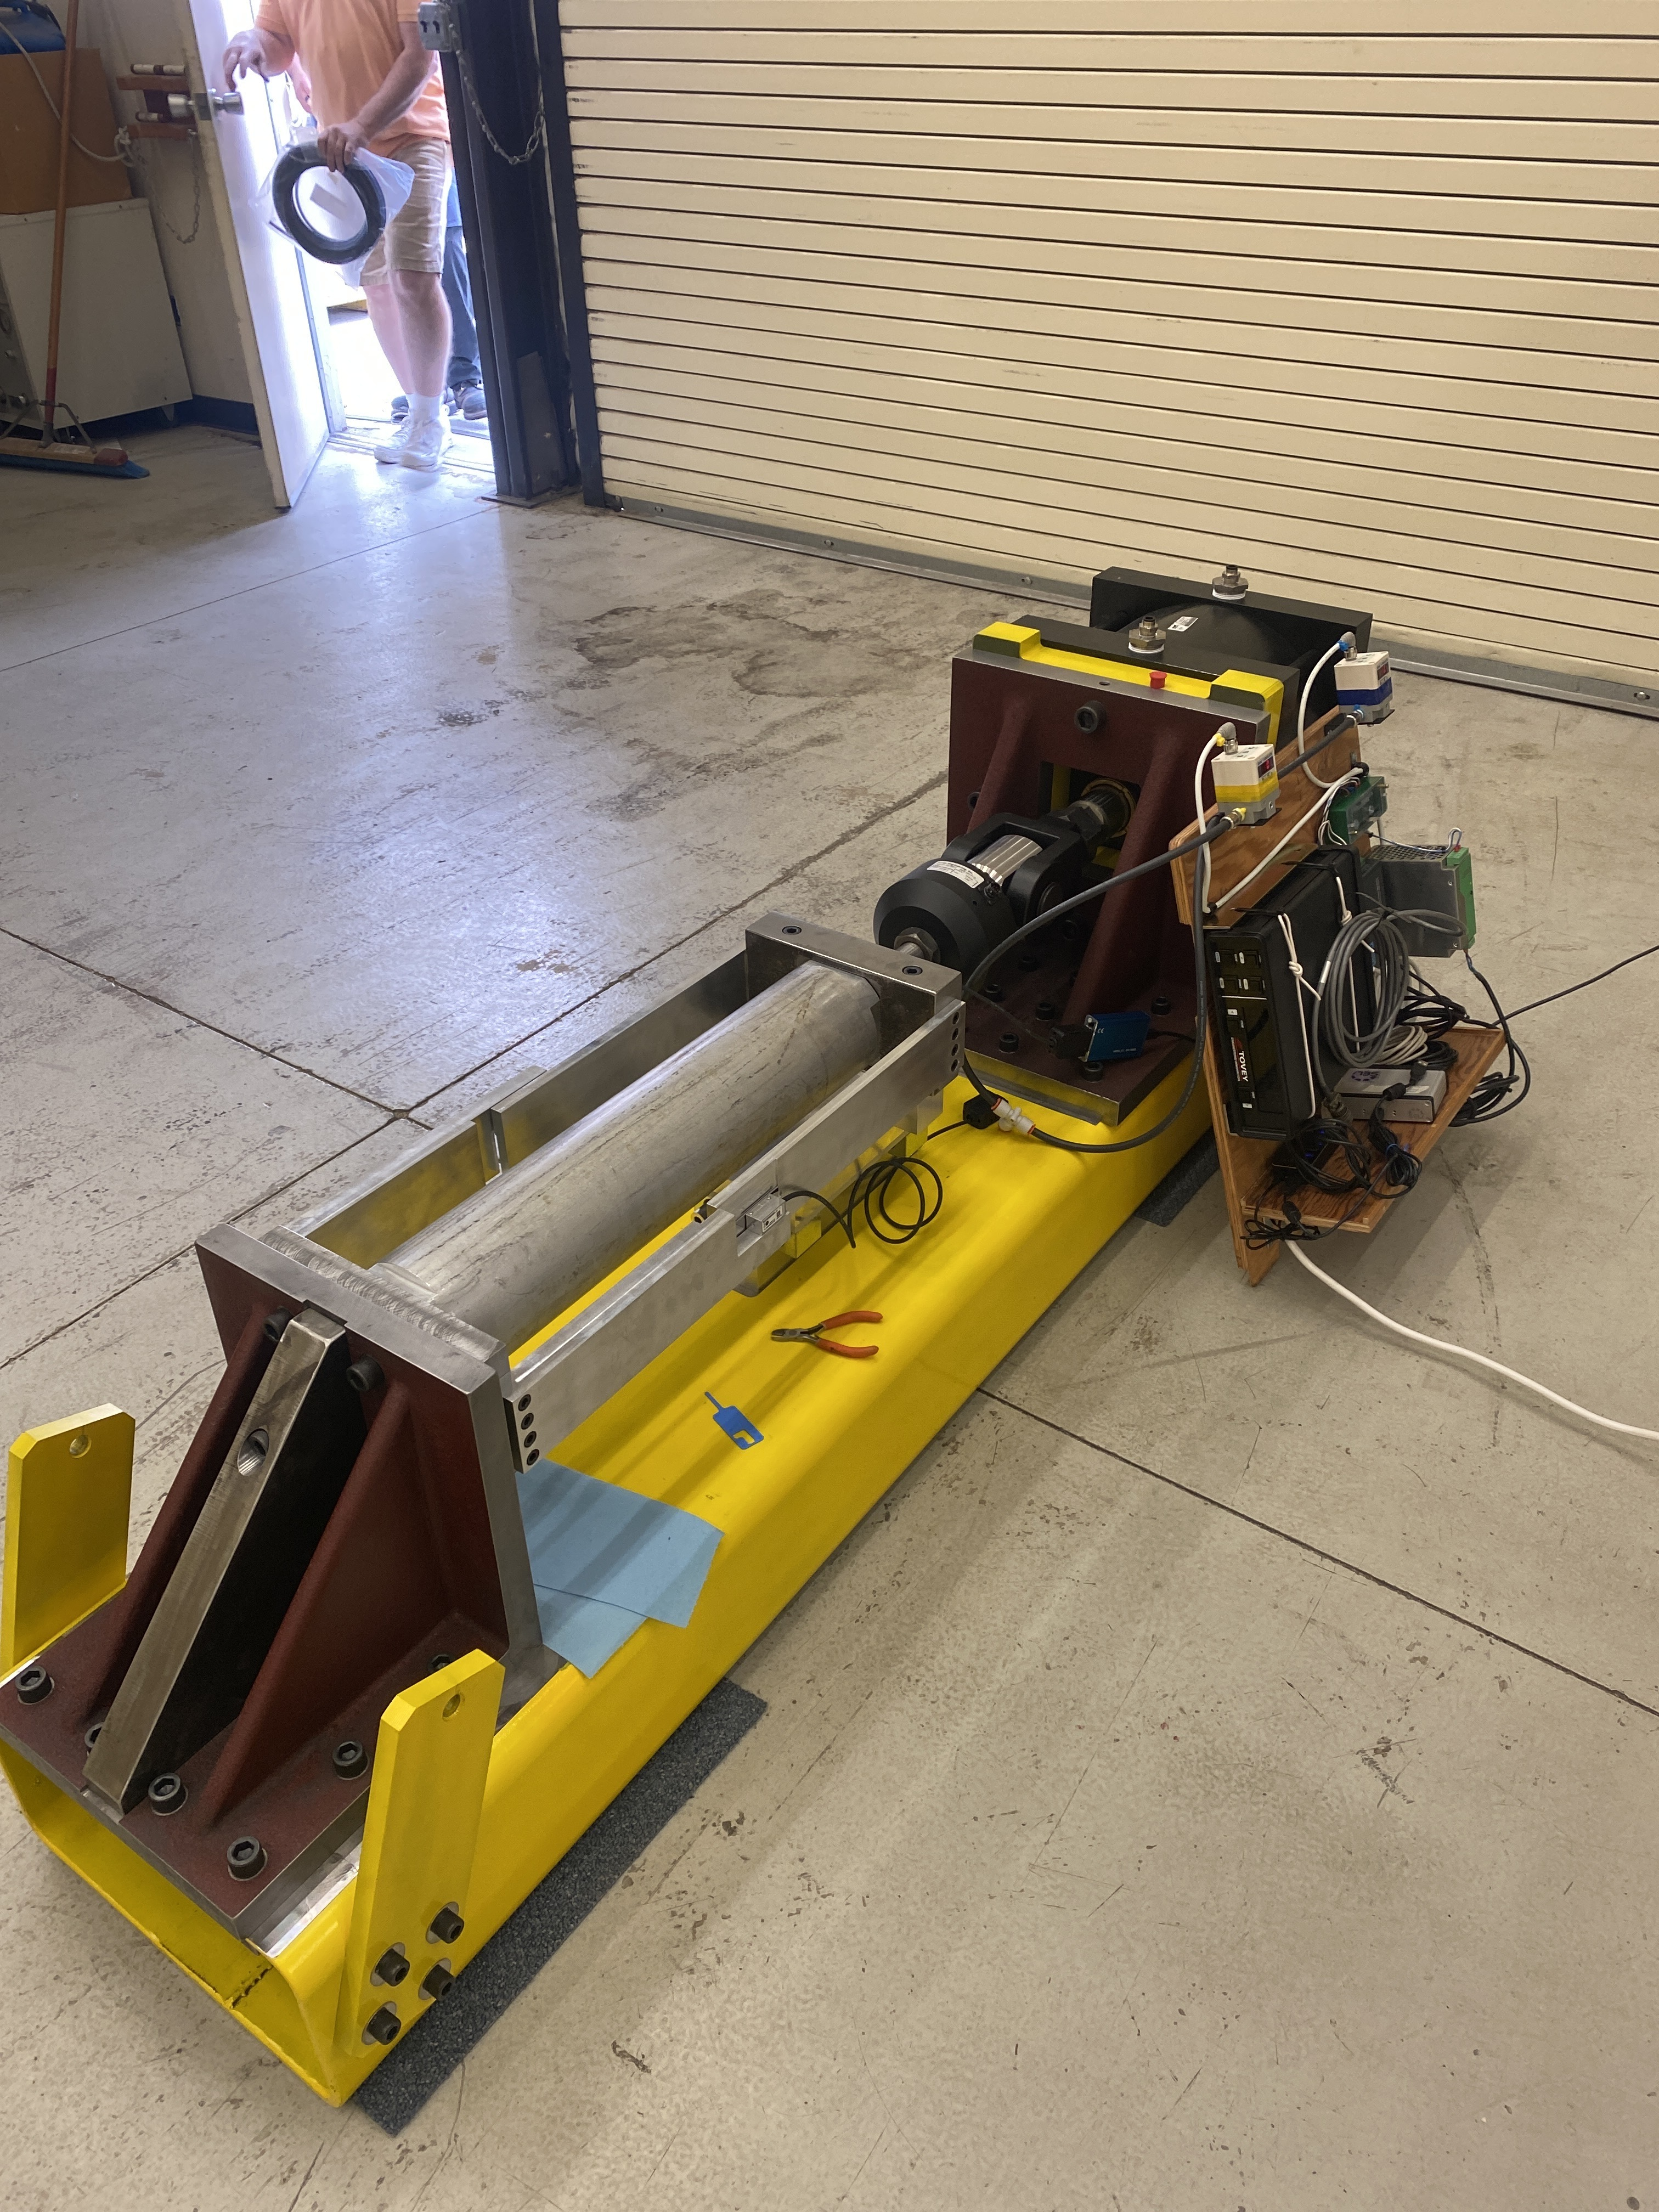
\includegraphics[width=3.12500in]{jira_imgs/3598.jpg}Test Rig with
Actuator:\\
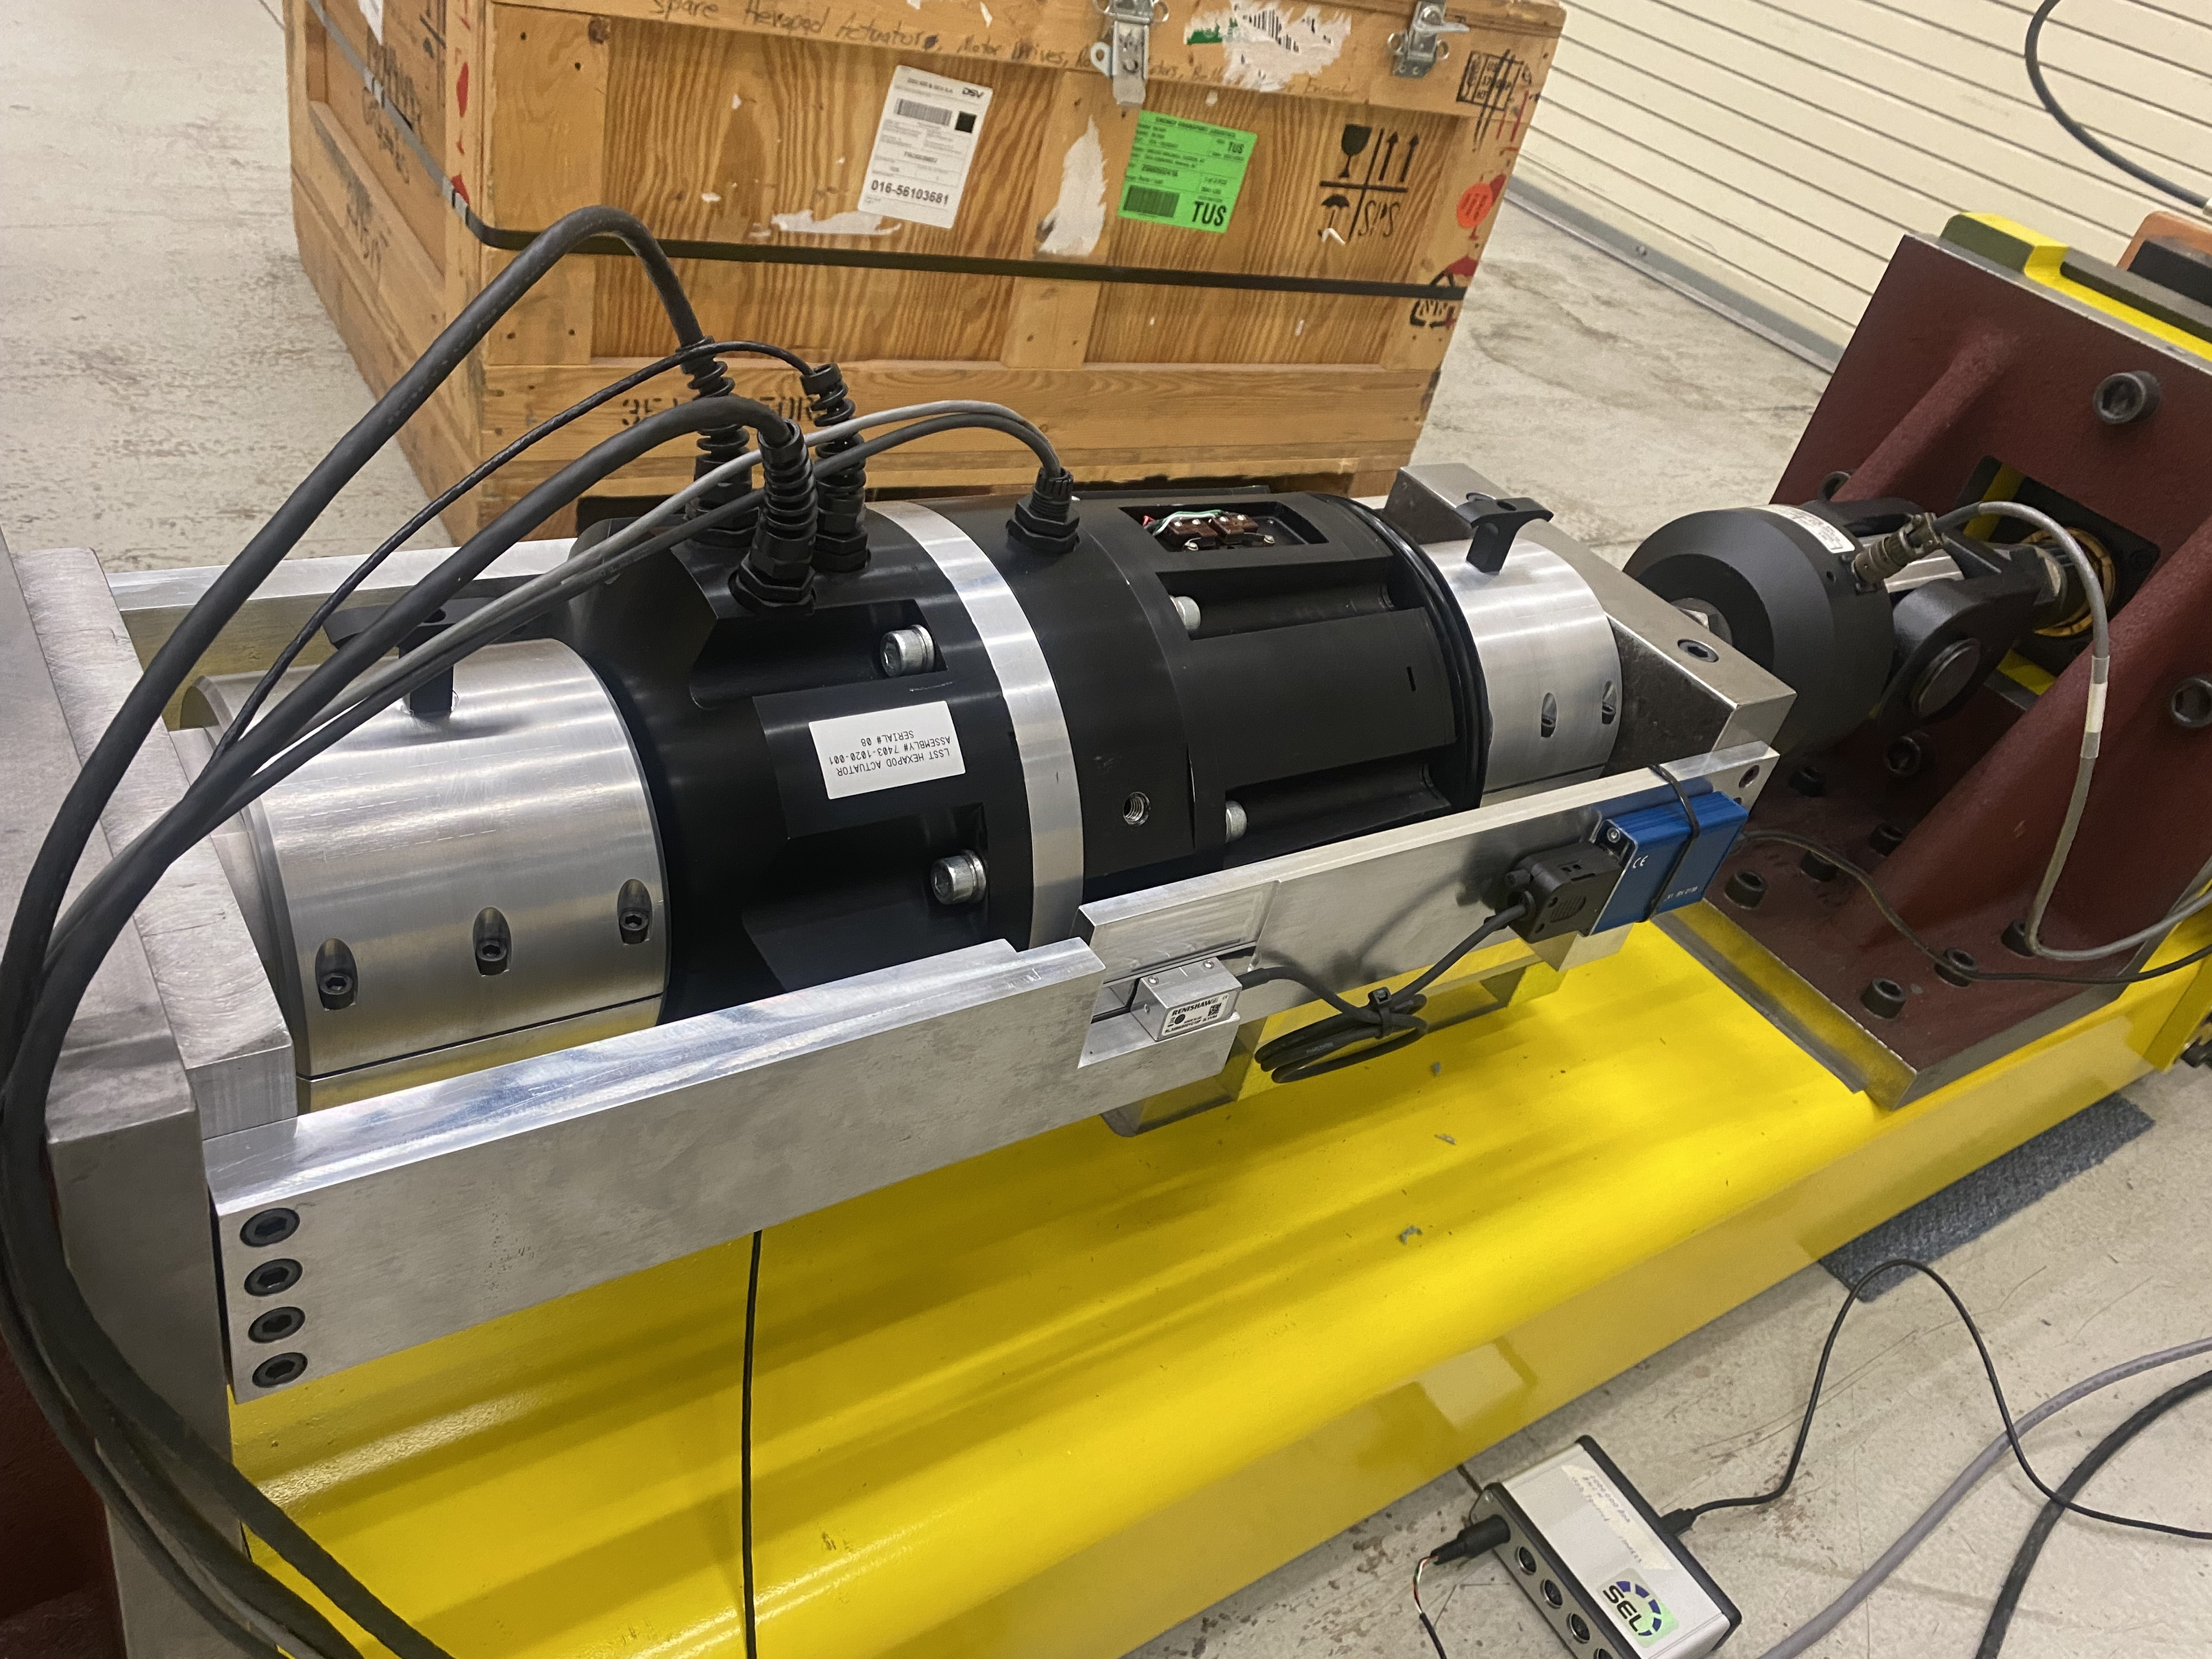
\includegraphics[width=3.12500in]{jira_imgs/3599.jpg}During
Installation, the bolts holding the surrogate/actuator to the interface
block and to the stiff back were torqued to 203 ft-lbs.

}
\begin{tabular}{p{2cm}p{14cm}}
\toprule
Step 3 & Step Execution Status: \textbf{ Pass } \\ \hline
\end{tabular}
 Description \\
{\footnotesize
Verify an air gauge is connected between the air supply and the air
valves.

}
\hdashrule[0.5ex]{\textwidth}{1pt}{3mm}
  Expected Result \\
{\footnotesize
\begin{itemize}
\tightlist
\item
  The air gauge is in position and capable of reading the psi value
  being supplied to the air valves.
\item
  The air gauge should initially show no air being supplied.
\end{itemize}

}
\hdashrule[0.5ex]{\textwidth}{1pt}{3mm}
  Actual Result \\
{\footnotesize
Although the air gauge in the control room was capable of reaching
150psi, for the purposes of these tests, the air supply was never set to
more than 100psi.~

}
\begin{tabular}{p{2cm}p{14cm}}
\toprule
Step 4 & Step Execution Status: \textbf{ Pass } \\ \hline
\end{tabular}
 Description \\
{\footnotesize
Verify the valves for tension and compression are capable of displaying
commanded voltage.~

}
\hdashrule[0.5ex]{\textwidth}{1pt}{3mm}
  Expected Result \\
{\footnotesize
Both air gauges are in place monitoring the output from both the tension
and compression air valves.

}
\hdashrule[0.5ex]{\textwidth}{1pt}{3mm}
  Actual Result \\
{\footnotesize
The valves for tension (blue) and compression (yellow):\\
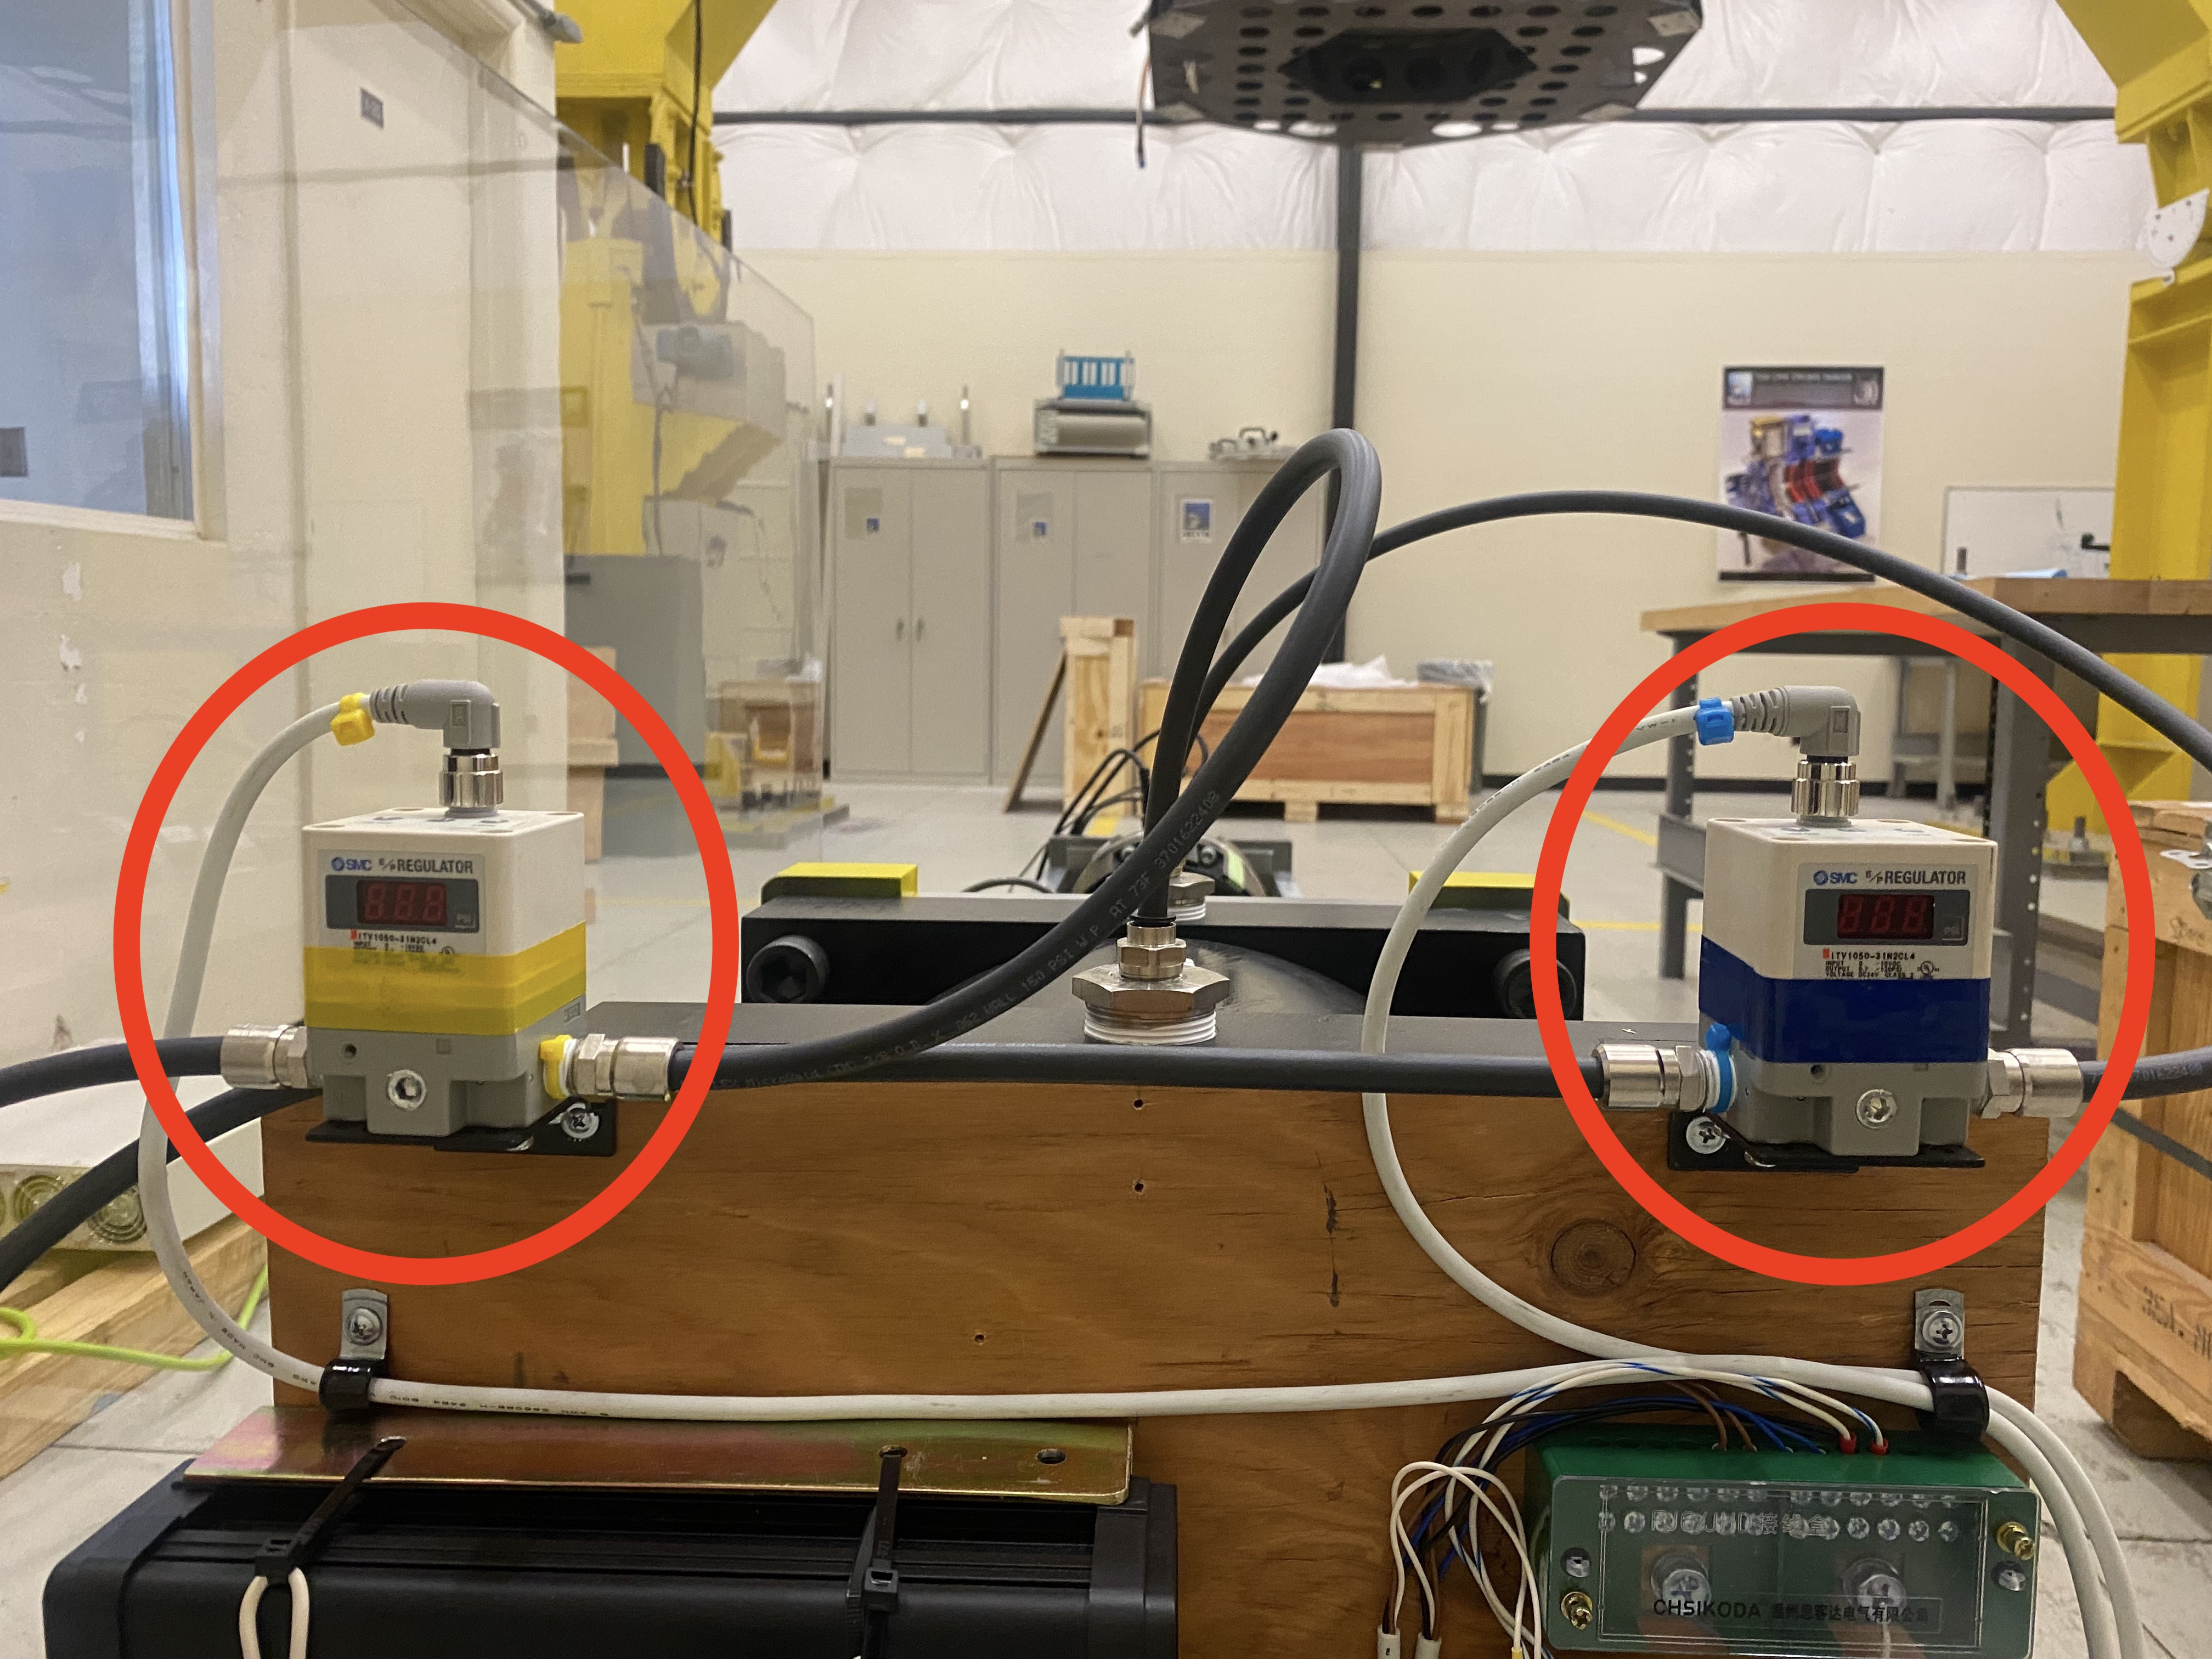
\includegraphics[width=3.12500in]{jira_imgs/3601.jpg}\\
When powered on, the valves displayed the voltage being commanded
through the Labview voltage command function, which correlates to how
much air is being supplied into the pneumatic cylinder. During set up,
the minimum and maximum voltages for each valve was set to 0 and 10V.

}
\begin{tabular}{p{2cm}p{14cm}}
\toprule
Step 5 & Step Execution Status: \textbf{ Pass } \\ \hline
\end{tabular}
 Description \\
{\footnotesize
Make the connection between the two sets of air valves and gauges and
the USB-4716 readout device.\\
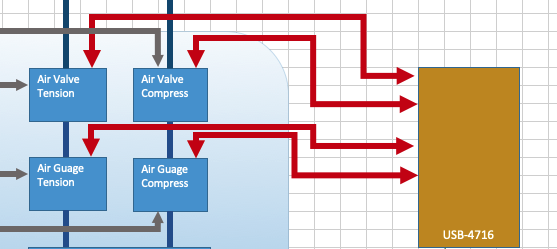
\includegraphics[width=3.12500in]{jira_imgs/3435.png}

}
\hdashrule[0.5ex]{\textwidth}{1pt}{3mm}
  Expected Result \\
{\footnotesize
The air valves and gauges are hooked up to the USB-4716 readout device.~

}
\hdashrule[0.5ex]{\textwidth}{1pt}{3mm}
  Actual Result \\
{\footnotesize
The tension and compression valves were connected to the USB-4716.
However, no additional gauges were placed in series between the valves
and the pneumatic cylinder as it was determined to be redundant and
unnecessary.

}
\begin{tabular}{p{2cm}p{14cm}}
\toprule
Step 6 & Step Execution Status: \textbf{ Pass } \\ \hline
\end{tabular}
 Description \\
{\footnotesize
Make the connection between the MB5U readout electronics and the
renishaw encoders.

}
\hdashrule[0.5ex]{\textwidth}{1pt}{3mm}
  Expected Result \\
{\footnotesize
The MB5U readouts are connected to the encoders.

}
\hdashrule[0.5ex]{\textwidth}{1pt}{3mm}
  Actual Result \\
{\footnotesize
The encoders were connected to the MB5U readout electronics. Both were
mounted onto the arms of the test fixture as seen in the picture
below.\\
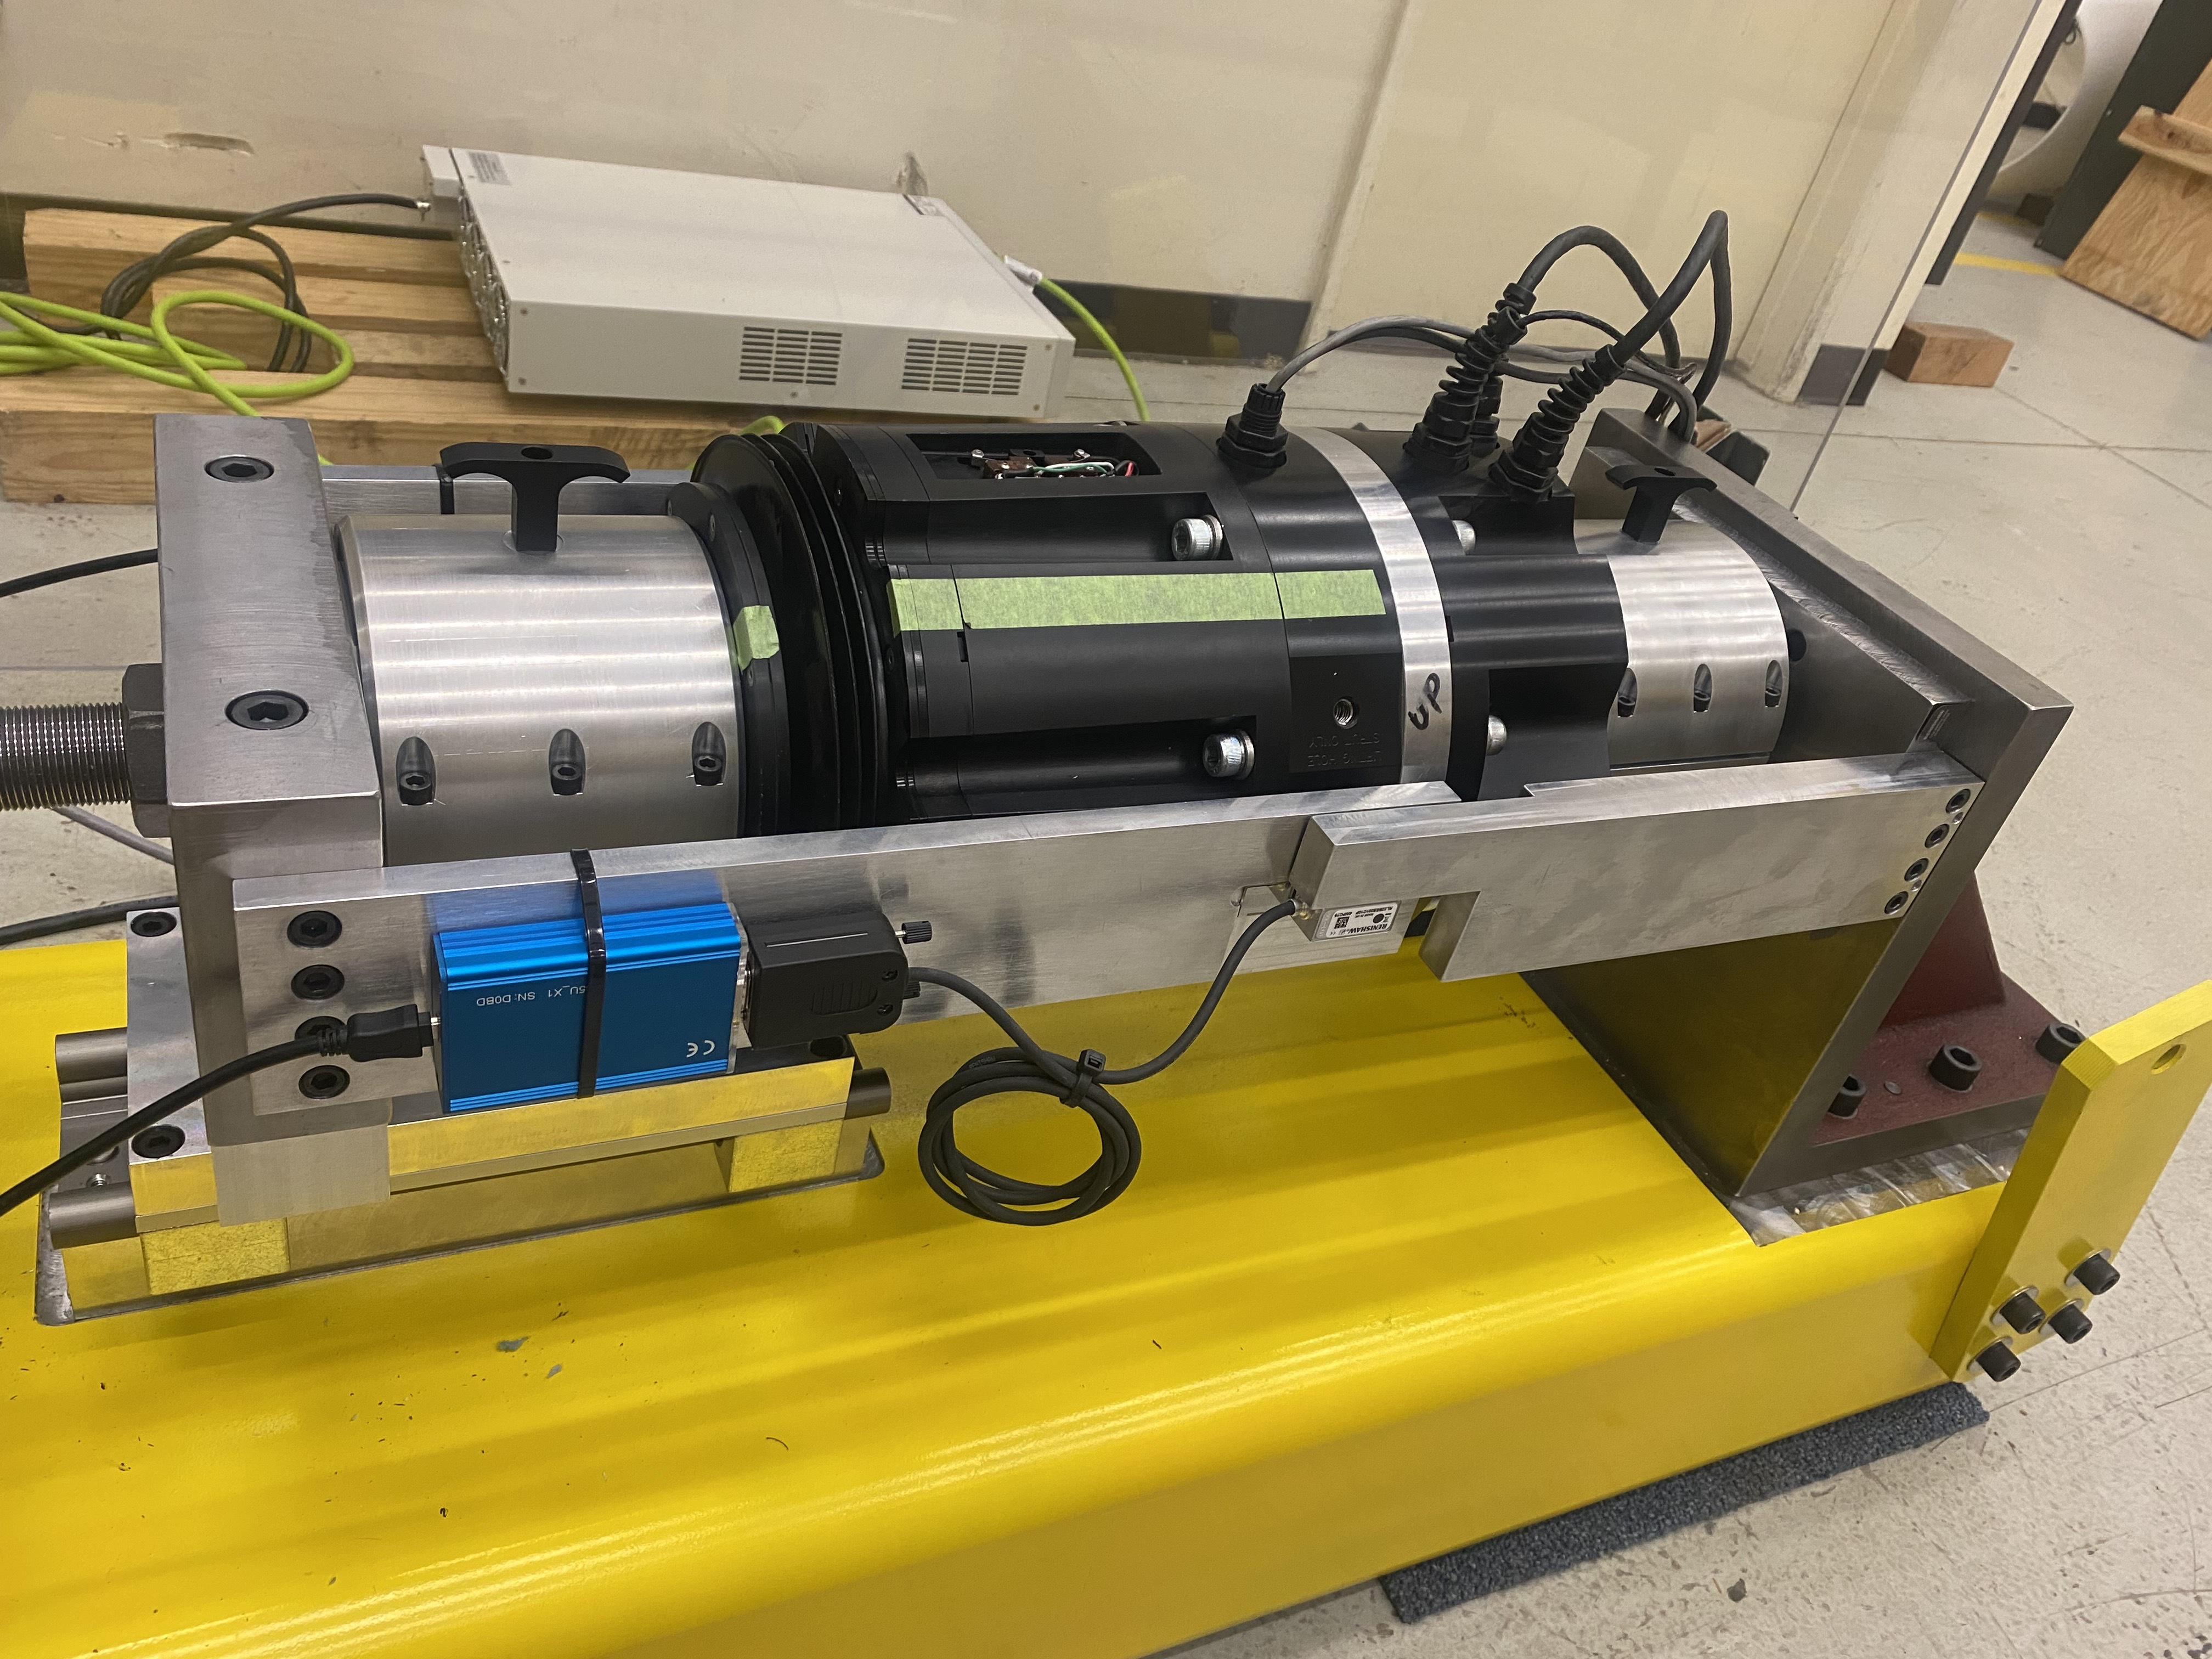
\includegraphics[width=3.12500in]{jira_imgs/3602.jpg}The configuration
that is being shown for this linear encoder and its reader was applied
in the same way to the other side with the other encoder and reader.

}
\begin{tabular}{p{2cm}p{14cm}}
\toprule
Step 7 & Step Execution Status: \textbf{ Pass } \\ \hline
\end{tabular}
 Description \\
{\footnotesize
Make the connection between the 9150 load cell readout electronic and
the load cell.

}
\hdashrule[0.5ex]{\textwidth}{1pt}{3mm}
  Expected Result \\
{\footnotesize
The load cell is connected to the load cell readout electronic.

}
\hdashrule[0.5ex]{\textwidth}{1pt}{3mm}
  Actual Result \\
{\footnotesize
As seen in the picture, the 9150 load cell readout electronic was
included on the mounted board with the rest of the electrical
connections. The load cell readout was directly connected to the load
cell.~\\
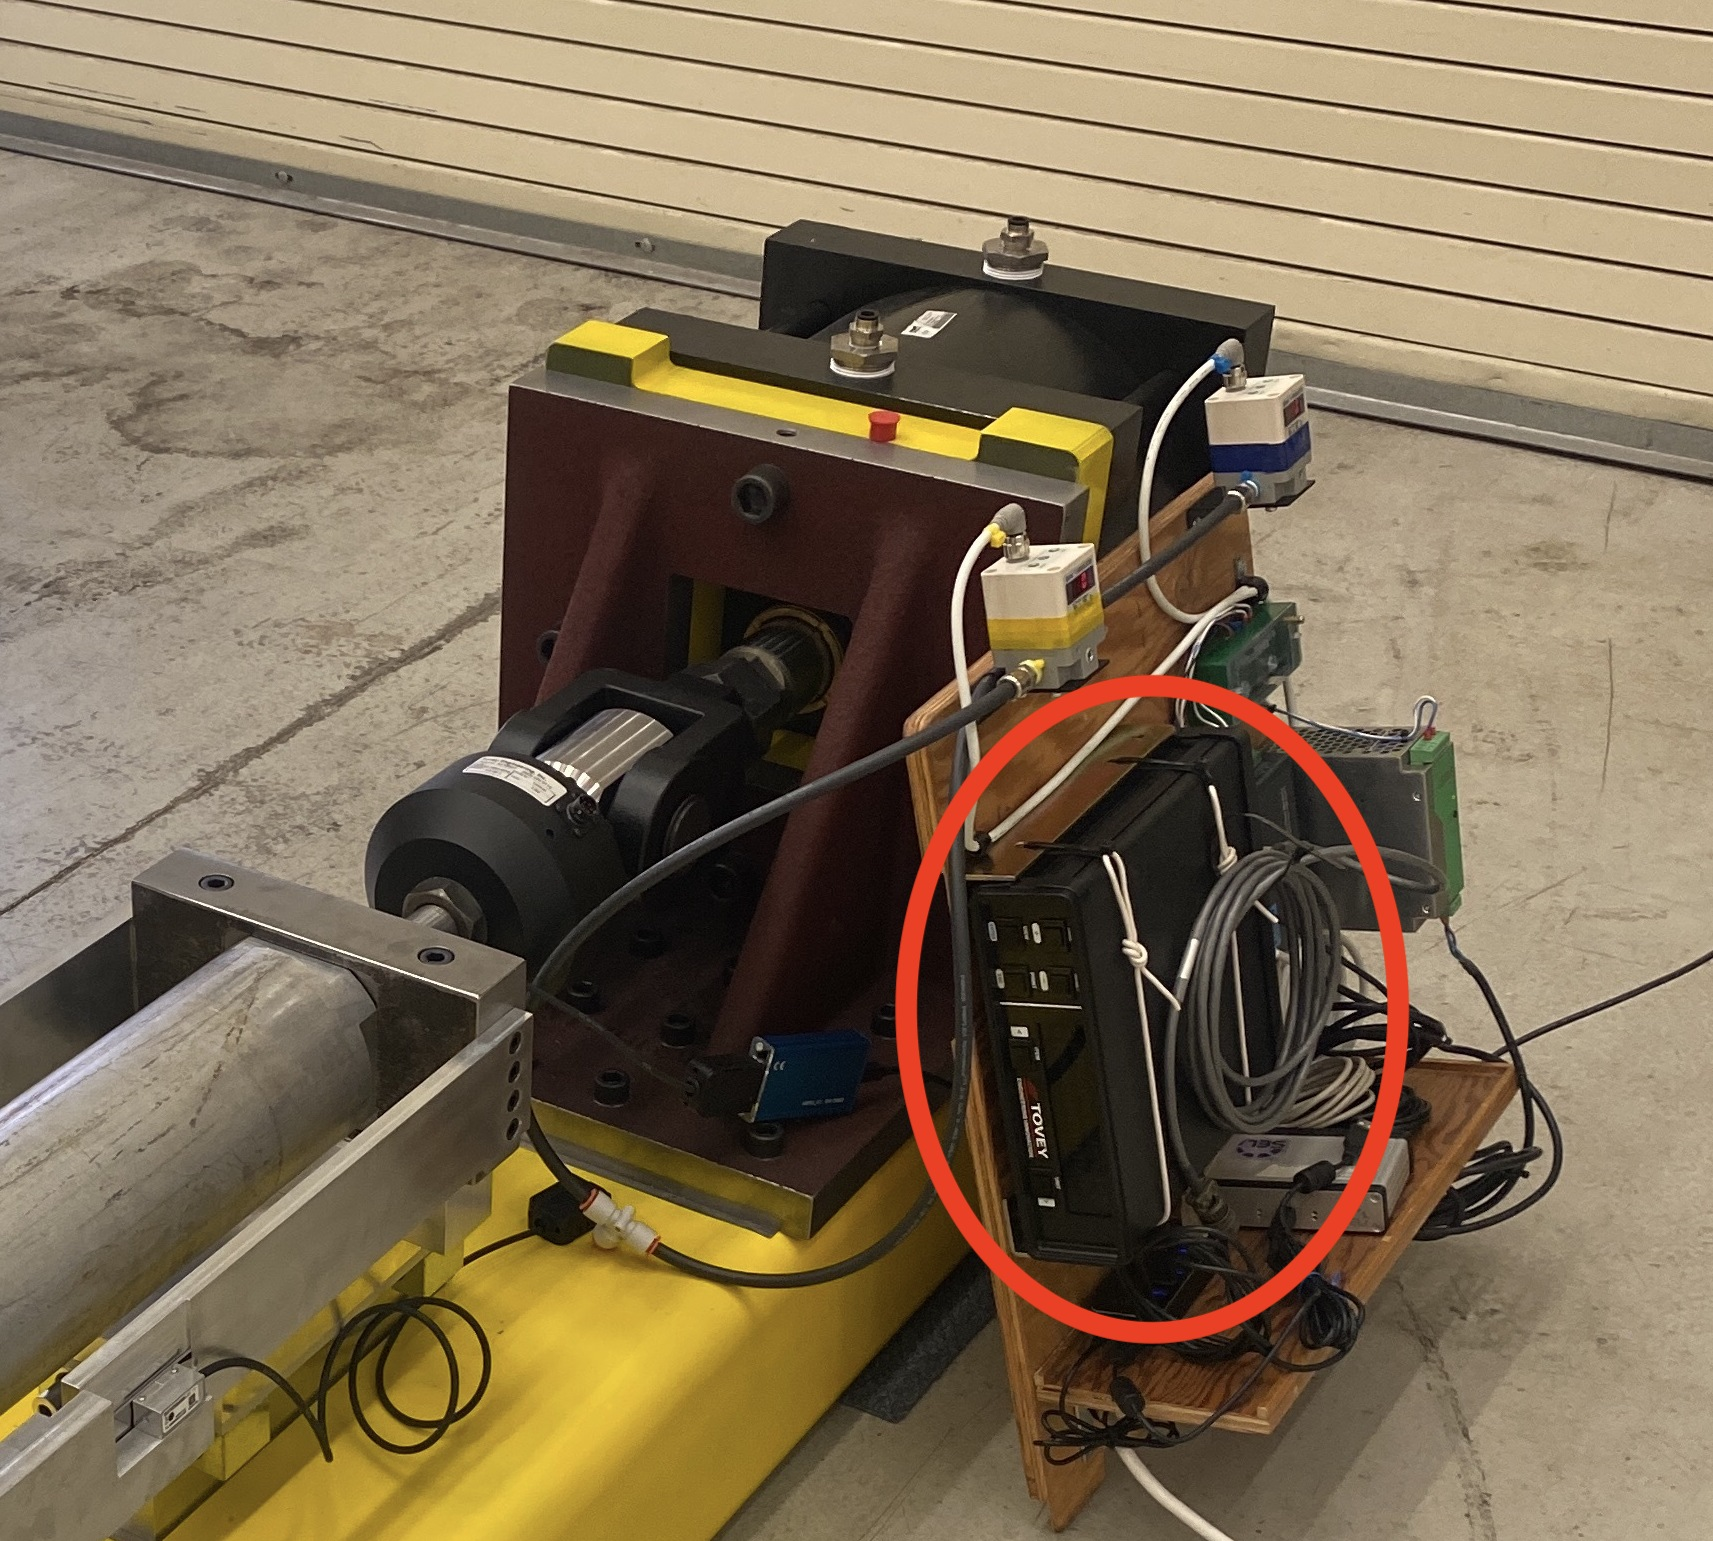
\includegraphics[width=3.12500in]{jira_imgs/3603.jpg}

}
\begin{tabular}{p{2cm}p{14cm}}
\toprule
Step 8 & Step Execution Status: \textbf{ Not Executed } \\ \hline
\end{tabular}
 Description \\
{\footnotesize
Make the connection between the Hexapod Actuator to the thermal
scanner.~

}
\hdashrule[0.5ex]{\textwidth}{1pt}{3mm}
  Expected Result \\
{\footnotesize
The thermal scanner is connected to the hexapod actuator.

}
\hdashrule[0.5ex]{\textwidth}{1pt}{3mm}
  Actual Result \\
{\footnotesize
This was not executed at the time of this test as the internal
temperature scanner cable was not available. However, an external
temperature sensor was able to be connected and readout by the RealTerm
application of the control computer.~

}
\begin{tabular}{p{2cm}p{14cm}}
\toprule
Step 9 & Step Execution Status: \textbf{ Pass } \\ \hline
\end{tabular}
 Description \\
{\footnotesize
Connect the following to the USB 3.0 Hub:

\begin{itemize}
\tightlist
\item
  (2) connections for MB5U Readout Electronic
\item
  USB-4716 Readout Device/Labjack T4
\item
  Temperature Readout
\item
  9150 Load Cell Readout Electronic
\end{itemize}

}
\hdashrule[0.5ex]{\textwidth}{1pt}{3mm}
  Expected Result \\
{\footnotesize
The USB 3.0 Hub is now connected to the readout electronics from the
previous steps.~

}
\hdashrule[0.5ex]{\textwidth}{1pt}{3mm}
  Actual Result \\
{\footnotesize
The USB 3.0 Hub was connected to the 2 MB5U Encoder readers, the
USB-4716 Readout Device for the pneumatic valves and the Tovey 9150 Load
Cell Readout. As mentioned in the previous step, the thermal scanner was
not connected.~

}
\begin{tabular}{p{2cm}p{14cm}}
\toprule
Step 10 & Step Execution Status: \textbf{ Pass } \\ \hline
\end{tabular}
 Description \\
{\footnotesize
Connect the laptop with LabVIEW software to the USB 3.0 Hub.

}
\hdashrule[0.5ex]{\textwidth}{1pt}{3mm}
  Expected Result \\
{\footnotesize
The Laptop is connected to the USB 3.0 Hub and to the subsequent readout
electronics.~

}
\hdashrule[0.5ex]{\textwidth}{1pt}{3mm}
  Actual Result \\
{\footnotesize
A cable was connected from the USB 3.0 Hub by the test rig to the laptop
with LabView in the control room.~

}
\begin{tabular}{p{2cm}p{14cm}}
\toprule
Step 11 & Step Execution Status: \textbf{ Pass } \\ \hline
\end{tabular}
 Description \\
{\footnotesize
Connect the laptop to the Copley Motor drive of the Control Box.

}
\hdashrule[0.5ex]{\textwidth}{1pt}{3mm}
  Expected Result \\
{\footnotesize
The laptop is connected to the control box.

}
\hdashrule[0.5ex]{\textwidth}{1pt}{3mm}
  Actual Result \\
{\footnotesize
The Control Box was set up next to the test rig and connected to the
same USB 3.0 Hub already connected to the laptop.~

}
\begin{tabular}{p{2cm}p{14cm}}
\toprule
Step 12 & Step Execution Status: \textbf{ Pass } \\ \hline
\end{tabular}
 Description \\
{\footnotesize
Set up the USB 3.0 Hub close to the test fixture and connect it to a
power source.~

}
\hdashrule[0.5ex]{\textwidth}{1pt}{3mm}
  Expected Result \\
{\footnotesize
The USB 3.0 Hub is connected and all readout devices are powered on.~

}
\hdashrule[0.5ex]{\textwidth}{1pt}{3mm}
  Actual Result \\
{\footnotesize
A power strip was attached to the electronics board and powered the USB
3.0 Hub.\\
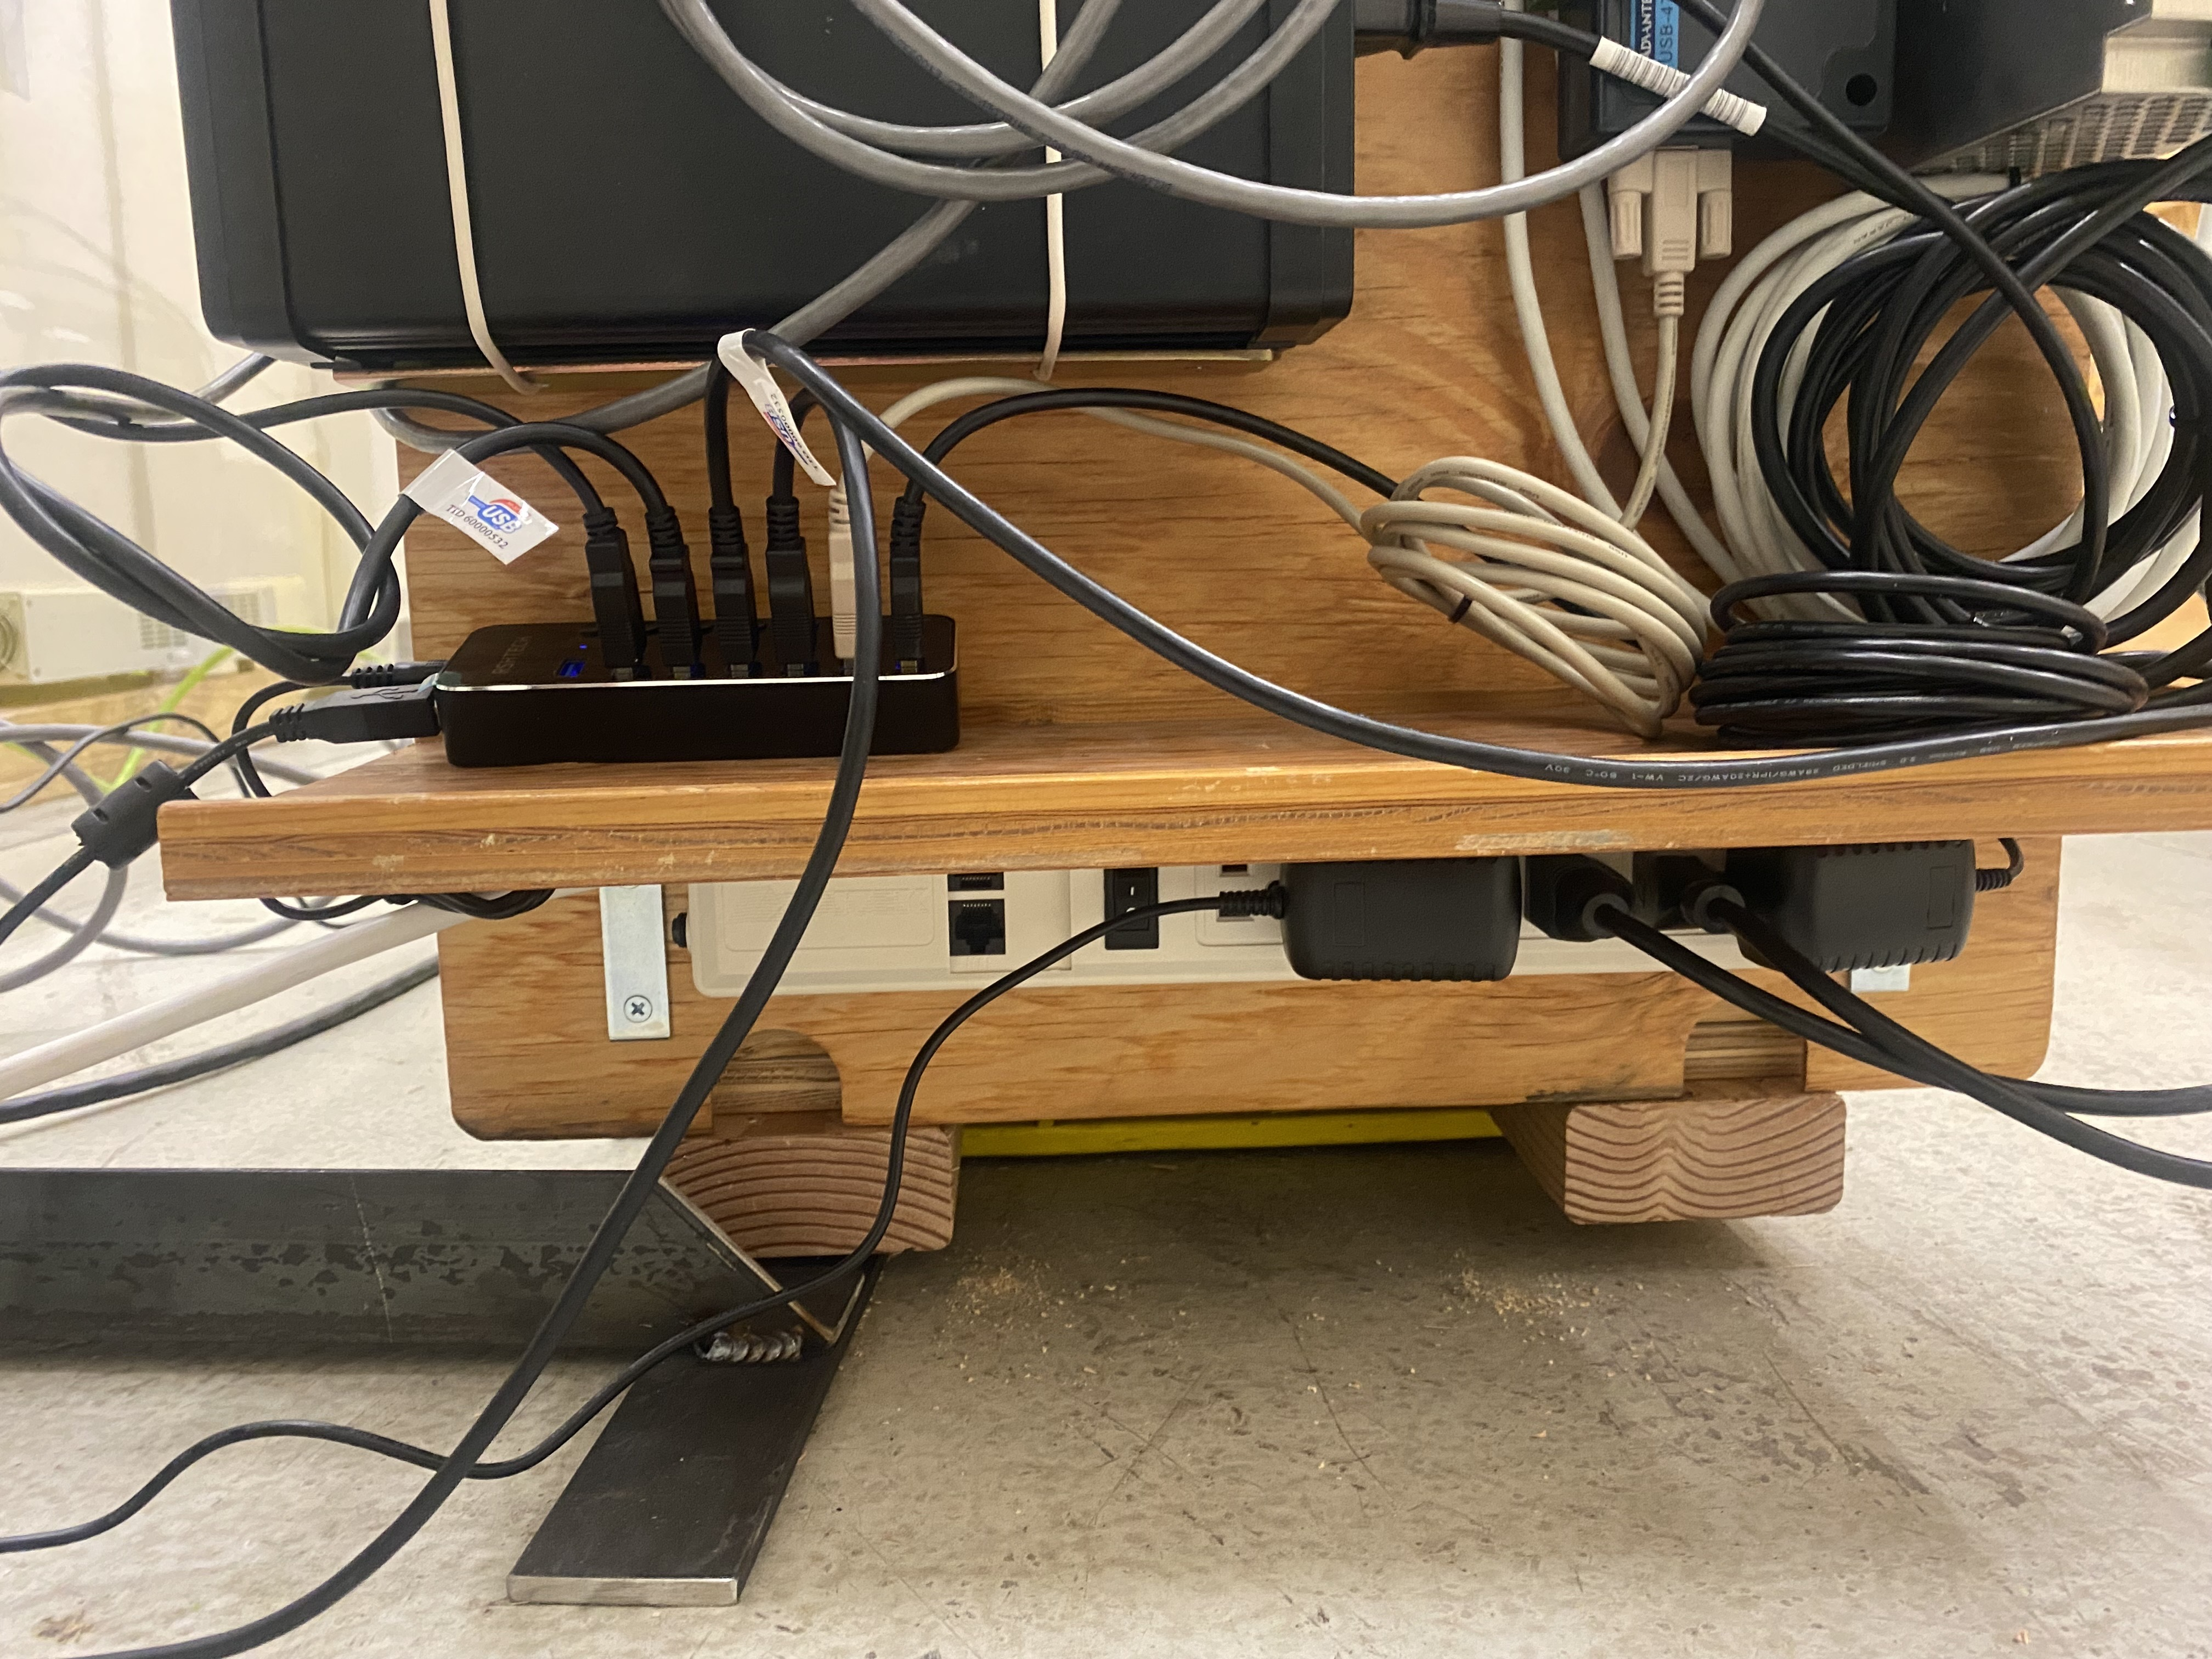
\includegraphics[width=3.12500in]{jira_imgs/3604.jpg}

}
\begin{tabular}{p{2cm}p{14cm}}
\toprule
Step 13 & Step Execution Status: \textbf{ Pass } \\ \hline
\end{tabular}
 Description \\
{\footnotesize
Verify that the output data from the readout devices are available on
the laptop.

}
\hdashrule[0.5ex]{\textwidth}{1pt}{3mm}
  Expected Result \\
{\footnotesize
The laptop is seen to be able to communicate with the readout devices.

}
\hdashrule[0.5ex]{\textwidth}{1pt}{3mm}
  Actual Result \\
{\footnotesize
Using LabView, we were able to confirm that we were able to read the
data from the encoder read heads.~

}
\begin{tabular}{p{2cm}p{14cm}}
\toprule
Step 14 & Step Execution Status: \textbf{ Pass } \\ \hline
\end{tabular}
 Description \\
{\footnotesize
Open Labview 2021 in the computer used for Test Setup.

}
\hdashrule[0.5ex]{\textwidth}{1pt}{3mm}
  Expected Result \\
{\footnotesize
Labview 2021 opens successfully.

}
\hdashrule[0.5ex]{\textwidth}{1pt}{3mm}
  Actual Result \\
{\footnotesize
LabView was available on the test computer.~

}
\begin{tabular}{p{2cm}p{14cm}}
\toprule
Step 15 & Step Execution Status: \textbf{ Pass } \\ \hline
\end{tabular}
 Description \\
{\footnotesize
Open the Labview VI files from the project directory including sub VIs-
Tovey Closed loop.vi, Voltage Regulation.vi and Biss Reader.vi

}
\hdashrule[0.5ex]{\textwidth}{1pt}{3mm}
  Expected Result \\
{\footnotesize
Front panel of VI and sub VI files open without any error.

}
\hdashrule[0.5ex]{\textwidth}{1pt}{3mm}
  Actual Result \\
{\footnotesize
The LabView VI files that we used were updated and renamed. The new
files can be found in the
\href{https://docushare.lsst.org/docushare/dsweb/View/Collection-13959}{Control
Software Files docushare collection}.

}
\begin{tabular}{p{2cm}p{14cm}}
\toprule
Step 16 & Step Execution Status: \textbf{ Pass } \\ \hline
\end{tabular}
 Description \\
{\footnotesize
Configure the Biss Reader.vi file with the appropriate configuration
file and following the IBISS operation manual.~

}
\hdashrule[0.5ex]{\textwidth}{1pt}{3mm}
  Expected Result \\
{\footnotesize
\href{https://jira.lsstcorp.org/rest/tests/1.0/attachment/3555}{BiSS\_config.cfg}
is loaded in the LabView configuration (Misc Tab under Load DLL). The
configuration file is based on the IBISS operation manual.

}
\hdashrule[0.5ex]{\textwidth}{1pt}{3mm}
  Actual Result \\
{\footnotesize
As stated in the previous step, the BISS Reader file has been modified.
As a result, the instructions for loading the DLL config file are more
straightforward. T

}
\begin{tabular}{p{2cm}p{14cm}}
\toprule
Step 17 & Step Execution Status: \textbf{ Pass } \\ \hline
\end{tabular}
 Description \\
{\footnotesize
Click Run button on the on the block diagram toolbar of the Labview VI
front panel.

}
\hdashrule[0.5ex]{\textwidth}{1pt}{3mm}
  Expected Result \\
{\footnotesize
LabView VI and ~associated sub Vi runs successfully. Initially all the
graphs and input values will be blank.

}
\hdashrule[0.5ex]{\textwidth}{1pt}{3mm}
  Actual Result \\
{\footnotesize
The LabView VI was able to be run without errors.

}
\begin{tabular}{p{2cm}p{14cm}}
\toprule
Step 18 & Step Execution Status: \textbf{ Not Executed } \\ \hline
\end{tabular}
 Description \\
{\footnotesize
Send a command through LabVIEW ~voltage Regulation.vi to set the voltage
on the compression valve only to 3V.

}
\hdashrule[0.5ex]{\textwidth}{1pt}{3mm}
  Expected Result \\
{\footnotesize
The command is accepted, the pneumatic valve shows the applied voltage
only on the compression valve and the applied compression force can be
seen on the LabView front panel Time vs Load graph.~

}
\hdashrule[0.5ex]{\textwidth}{1pt}{3mm}
  Actual Result \\
{\footnotesize
During the Hexapod Initial Validation test
(\href{https://jira.lsstcorp.org/secure/Tests.jspa\#/testPlayer/testExecution/LVV-E2728}{LVV-E2728}),
we verified that we were able to apply voltages for both the tension and
compression valves through Labview and their corresponding values in
force being applied.~

}
\begin{tabular}{p{2cm}p{14cm}}
\toprule
Step 19 & Step Execution Status: \textbf{ Not Executed } \\ \hline
\end{tabular}
 Description \\
{\footnotesize
Send a command through LabVIEW voltage Regulation.vi to reset the
compression valve to 0V.

}
\hdashrule[0.5ex]{\textwidth}{1pt}{3mm}
  Expected Result \\
{\footnotesize
The command is accepted. The applied force can be seen as zero load on
the LabView front panel Time vs Load graph. Load Cell Reader also shows
zero load.

}
\hdashrule[0.5ex]{\textwidth}{1pt}{3mm}
  Actual Result \\
{\footnotesize
During the Hexapod Initial Validation test
(\href{https://jira.lsstcorp.org/secure/Tests.jspa\#/testPlayer/testExecution/LVV-E2728}{LVV-E2728}),
we verified that we were able to apply voltages for both the tension and
compression valves through Labview and their corresponding values in
force being applied.

}
\begin{tabular}{p{2cm}p{14cm}}
\toprule
Step 20 & Step Execution Status: \textbf{ Not Executed } \\ \hline
\end{tabular}
 Description \\
{\footnotesize
Send a command through LabVIEW to reset the tension valve to 3V.

}
\hdashrule[0.5ex]{\textwidth}{1pt}{3mm}
  Expected Result \\
{\footnotesize
The command is accepted, the readout electronic shows the applied
voltage only on the tension valve and the applied tension force can be
seen on the LabView front panel Time vs Load graph.

}
\hdashrule[0.5ex]{\textwidth}{1pt}{3mm}
  Actual Result \\
{\footnotesize
During the Hexapod Initial Validation test
(\href{https://jira.lsstcorp.org/secure/Tests.jspa\#/testPlayer/testExecution/LVV-E2728}{LVV-E2728}),
we verified that we were able to apply voltages for both the tension and
compression valves through Labview and their corresponding values in
force being applied.

}
\begin{tabular}{p{2cm}p{14cm}}
\toprule
Step 21 & Step Execution Status: \textbf{ Not Executed } \\ \hline
\end{tabular}
 Description \\
{\footnotesize
Send a command through LabVIEW to reset the tension valve to 0V.

}
\hdashrule[0.5ex]{\textwidth}{1pt}{3mm}
  Expected Result \\
{\footnotesize
The command is accepted, the readout electronic no longer shows the
applied voltage on the tension valve and there is no longer any tension
force on the LabView front panel Time vs Load graph.

}
\hdashrule[0.5ex]{\textwidth}{1pt}{3mm}
  Actual Result \\
{\footnotesize
During the Hexapod Initial Validation test
(\href{https://jira.lsstcorp.org/secure/Tests.jspa\#/testPlayer/testExecution/LVV-E2728}{LVV-E2728}),
we verified that we were able to apply voltages for both the tension and
compression valves through Labview and their corresponding values in
force being applied.

}
\begin{tabular}{p{2cm}p{14cm}}
\toprule
Step 22 & Step Execution Status: \textbf{ Pass } \\ \hline
\end{tabular}
 Description \\
{\footnotesize
Verify the laptop is reading the renishaw scales usinthe Biss Reader.vi
file and determine the zero stroke position.

}
\hdashrule[0.5ex]{\textwidth}{1pt}{3mm}
  Test Data \\
 {\footnotesize
\textbf{Note:~}Moog's original test procedure cited the zero position to
be at 40mm since the full length was 80mm.

}
\hdashrule[0.5ex]{\textwidth}{1pt}{3mm}
  Expected Result \\
{\footnotesize
40mm encoder readings shown in Labview front panel of the .vi file.~\\
The zero stroke position has been determined and can be used as a
reference for the offset of future moves.

}
\hdashrule[0.5ex]{\textwidth}{1pt}{3mm}
  Actual Result \\
{\footnotesize
Using the modified Encoder A (D13B) and Load Cell.vi and Encoder B
(D0BD).vi, we verified the position of the readings of each of the
external encoders. Then using the copley control software, we verified
the position of the external encoders when the actuator was in the
center stroke position. As documented in the next steps, we saw both
encoders reading about 39.5mm

}
\begin{tabular}{p{2cm}p{14cm}}
\toprule
Step 23 & Step Execution Status: \textbf{ Pass } \\ \hline
\end{tabular}
 Description \\
{\footnotesize
Using the Copley Software, drive the actuator to the positive limit
switch and take note of the values measured by the Copley Software and
the Encoder Readings.

}
\hdashrule[0.5ex]{\textwidth}{1pt}{3mm}
  Expected Result \\
{\footnotesize
The actuator is able to hit the positive limit switch and the values are
recorded.

}
\hdashrule[0.5ex]{\textwidth}{1pt}{3mm}
  Actual Result \\
{\footnotesize
The positive limit switch was reached reading the following values:

\begin{itemize}
\tightlist
\item
  Copley Software: Active Load Position = -25.904mm
\item
  Encoder A (D13B) = 25.390mm
\item
  Encoder B (D0BD) = 25.068mm
\end{itemize}

Note: No load was applied during this step

}
\begin{tabular}{p{2cm}p{14cm}}
\toprule
Step 24 & Step Execution Status: \textbf{ Pass } \\ \hline
\end{tabular}
 Description \\
{\footnotesize
Using the Copley Software, drive the actuator to the negative limit
switch and take note of the values measured by the Copley Software and
the Encoder Readings.

}
\hdashrule[0.5ex]{\textwidth}{1pt}{3mm}
  Expected Result \\
{\footnotesize
The actuator is able to hit the negative limit switch and the values are
recorded.

}
\hdashrule[0.5ex]{\textwidth}{1pt}{3mm}
  Actual Result \\
{\footnotesize
The negative limit switch was reached reading the following values:

\begin{itemize}
\tightlist
\item
  Copley Software: Active Load Position = -54.501mm
\item
  Encoder A (D13B) = 53.982mm
\item
  Encoder B (D0BD) = 53.645mm
\end{itemize}

Note: No load was applied during this step\\[2\baselineskip]The overall
travel = 28.597mm\\
The zero position should be set to exactly half the overall travel from
each limit switch (14.298mm)\\
Therefore, the zero position as reported by the Copley =
\textbf{-40.202mm or -40202000 counts}

}

\paragraph{ LVV-T2427 - Hexapod - Actuator Back Driving Test }\mbox{}\\

Version \textbf{1}.
Status \textbf{Approved}.
Open  \href{https://jira.lsstcorp.org/secure/Tests.jspa#/testCase/LVV-T2427}{\textit{ LVV-T2427 } }
test case in Jira.

The objective of this test case is to verify that removing the power
from an actuator will not cause the actuator to back drive even with the
application of different loads.

\textbf{ Preconditions}:\\
Proofing 200\% load test should be performed before running the
back-driving test.~

Execution status: {\bf Pass }

Final comment:\\The proofing 200\% load test will not be conducted as part of this test
cycle. Therefore, it was not a pre-requisite to executing this test
case. See
\href{https://jira.lsstcorp.org/secure/Tests.jspa\#/testPlayer/testExecution/LVV-E2728}{LVV-E2728}.\\[2\baselineskip]During
MOOG's original test, the back driving was determined by reading the
internal rotary encoder and therefore was measured in counts. During
this test, the displacement was measured by the external linear encoders
and was measured in mm. As seen in the results, the total displacement
by either encoder when applying loads never exceeded 0.32mm. The results
were agreed to be sufficient to repeat this test on the modified
actuator.


Detailed steps results:

\begin{tabular}{p{2cm}p{14cm}}
\toprule
Step 1.1 & Step Execution Status: \textbf{ Pass } \\ \hline
\end{tabular}
 Description \\
{\footnotesize
Open Labview 2021 in the computer used for Test Setup.

}
\hdashrule[0.5ex]{\textwidth}{1pt}{3mm}
  Test Data \\
 {\footnotesize
\textbf{Note:~}The first three steps are conditional because these steps
are included as part of the Test Setup procedure and may not be
necessary if LabView is still open.

}
\hdashrule[0.5ex]{\textwidth}{1pt}{3mm}
  Expected Result \\
{\footnotesize
Labview 2021 opens successfully.

}
\hdashrule[0.5ex]{\textwidth}{1pt}{3mm}
  Actual Result \\
{\footnotesize
Labview has been opened.~

}
\begin{tabular}{p{2cm}p{14cm}}
\toprule
Step 1.2 & Step Execution Status: \textbf{ Pass } \\ \hline
\end{tabular}
 Description \\
{\footnotesize
Run the following VI's:

\begin{itemize}
\tightlist
\item
  Encoder A (D13B) and Load Cell.vi
\item
  Encoder B (D0BD).vi
\end{itemize}

}
\hdashrule[0.5ex]{\textwidth}{1pt}{3mm}
  Test Data \\
 {\footnotesize
\textbf{Note:~}Each vi is responsible for reading one encoder.

}
\hdashrule[0.5ex]{\textwidth}{1pt}{3mm}
  Expected Result \\
{\footnotesize
Front panel of VI's open without any error.

}
\hdashrule[0.5ex]{\textwidth}{1pt}{3mm}
  Actual Result \\
{\footnotesize
The VI's were opened with no issue.

}
\begin{tabular}{p{2cm}p{14cm}}
\toprule
Step 1.3 & Step Execution Status: \textbf{ Pass } \\ \hline
\end{tabular}
 Description \\
{\footnotesize
Click Run button on the block diagram toolbar of the Labview VI front
panel.

}
\hdashrule[0.5ex]{\textwidth}{1pt}{3mm}
  Expected Result \\
{\footnotesize
LabView VI and associated sub Vi runs successfully. The graphs should
start to be populated with data once the run button is pressed.

}
\hdashrule[0.5ex]{\textwidth}{1pt}{3mm}
  Actual Result \\
{\footnotesize
The VI's were able to run.

}
\begin{tabular}{p{2cm}p{14cm}}
\toprule
Step 1.4 & Step Execution Status: \textbf{ Pass } \\ \hline
\end{tabular}
 Description \\
{\footnotesize
Record the starting position of the actuator using the external
encoders.

}
\hdashrule[0.5ex]{\textwidth}{1pt}{3mm}
  Test Data \\
 {\footnotesize
\textbf{Note:~}The Copley software will display a value based on the
reading from its internal encoder, which may be useful to take note of.
However, the readings reported by the external encoders will validate
the reading of the internal encoder.

}
\hdashrule[0.5ex]{\textwidth}{1pt}{3mm}
  Expected Result \\
{\footnotesize
The actuator position is determined by the external encoders.

}
\hdashrule[0.5ex]{\textwidth}{1pt}{3mm}
  Actual Result \\
{\footnotesize
During the Actuator Test Set up test, the zero position of the actuator
was -40.202mm as measured by the Copley Control Software. The actuator
was commanded to this zero position where the readings of the external
encoders read:

\begin{itemize}
\tightlist
\item
  Encoder A = 39.7102mm
\item
  Encoder B = 39.3261mm
\end{itemize}

}
\begin{tabular}{p{2cm}p{14cm}}
\toprule
Step 1.5 & Step Execution Status: \textbf{ Pass } \\ \hline
\end{tabular}
 Description \\
{\footnotesize
Make sure motor drive is disabled using Copley software and the control
box.~

}
\hdashrule[0.5ex]{\textwidth}{1pt}{3mm}
  Expected Result \\
{\footnotesize
Motor drive is disabled.~

}
\hdashrule[0.5ex]{\textwidth}{1pt}{3mm}
  Actual Result \\
{\footnotesize
E-stop was pressed which disabled the control software but still allowed
us to read the values being reported.

}
\begin{tabular}{p{2cm}p{14cm}}
\toprule
Step 1.6 & Step Execution Status: \textbf{ Pass } \\ \hline
\end{tabular}
 Description \\
{\footnotesize
Slowly apply an increasing {Tension}⁠ ~force of +/-37.5kN.~

}
\hdashrule[0.5ex]{\textwidth}{1pt}{3mm}
  Test Data \\
 {\footnotesize
\textbf{Note:~}Set the {Tension}⁠ valve to 5.48V in order to apply
+/-37.5kN of force.

}
\hdashrule[0.5ex]{\textwidth}{1pt}{3mm}
  Expected Result \\
{\footnotesize
Load cell reader shows the applied +/-37.5kN {Tension}⁠~ force.\\
LabView displays the voltage being applied.

}
\hdashrule[0.5ex]{\textwidth}{1pt}{3mm}
  Actual Result \\
{\footnotesize
With 90psi, a tension force of +37.5kN was applied by setting Channel 1
= 5.7V and Channel 0 = 0V.\\
This can be seen in the Tension (0-38kN) sheet of the \emph{Back Drive
Test Results - Unmodified Actuator.xlsx~}file.

}
\begin{tabular}{p{2cm}p{14cm}}
\toprule
Step 1.7 & Step Execution Status: \textbf{ Pass } \\ \hline
\end{tabular}
 Description \\
{\footnotesize
Record the displacement of the actuator using the external encoder
readings.

}
\hdashrule[0.5ex]{\textwidth}{1pt}{3mm}
  Test Data \\
 {\footnotesize
\textbf{Note:~}The Copley software will display a value based on the
reading from its internal encoder, which may be useful to take note of.
However, the readings reported by the external encoders will validate
the reading of the internal encoder.

}
\hdashrule[0.5ex]{\textwidth}{1pt}{3mm}
  Expected Result \\
{\footnotesize
The final position of the actuator has been determined.\\
If the actuator position has changed significantly (\textgreater{}10
counts or 0.36 deg of motor rotation), the actuator has back-driven.

}
\hdashrule[0.5ex]{\textwidth}{1pt}{3mm}
  Actual Result \\
{\footnotesize
When full tension load was applied, the readings of the external
encoders read:

\begin{itemize}
\tightlist
\item
  Encoder A = 40.028mm
\item
  Encoder B = 39.625mm
\end{itemize}

This can be seen in the Tension (38kN) sheet of the \emph{Back Drive
Test Results - Unmodified Actuator.xlsx~}file.

}
\begin{tabular}{p{2cm}p{14cm}}
\toprule
Step 1.8 & Step Execution Status: \textbf{ Pass } \\ \hline
\end{tabular}
 Description \\
{\footnotesize
Confirm that there are no other signs of gross actuator motion.

}
\hdashrule[0.5ex]{\textwidth}{1pt}{3mm}
  Expected Result \\
{\footnotesize
No visual movement, significant motion of the internal linear encoder or
external linear test encoders beyond expected actuator compliance
recorded in the LabView displacement graphs.~

}
\hdashrule[0.5ex]{\textwidth}{1pt}{3mm}
  Actual Result \\
{\footnotesize
Visually, the position of the actuator remained in the center position.

}
\begin{tabular}{p{2cm}p{14cm}}
\toprule
Step 1.9 & Step Execution Status: \textbf{ Pass } \\ \hline
\end{tabular}
 Description \\
{\footnotesize
Reduce the {Tension}⁠ ~force to back to zero load.

}
\hdashrule[0.5ex]{\textwidth}{1pt}{3mm}
  Test Data \\
 {\footnotesize
\textbf{Note:~}In order to reset the load to zero, both the valves
should be set to 0V.

}
\hdashrule[0.5ex]{\textwidth}{1pt}{3mm}
  Expected Result \\
{\footnotesize
{Tension}⁠~ force removed and load cell reading in the lab-view graph
and load cell reader showing zero load.

}
\hdashrule[0.5ex]{\textwidth}{1pt}{3mm}
  Actual Result \\
{\footnotesize
Zero load was applied to the actuator by setting Channel 1 = Channel 0 =
0V.\\
With zero load, the Copley's Active Load Position = -0.00621mm

}
\begin{tabular}{p{2cm}p{14cm}}
\toprule
Step 2.0 & Step Execution Status: \textbf{ Pass } \\ \hline
\end{tabular}
 Description \\
{\footnotesize
Record the displacement of the actuator using the external encoder
readings.

}
\hdashrule[0.5ex]{\textwidth}{1pt}{3mm}
  Test Data \\
 {\footnotesize
\textbf{Note:~}The Copley software will display a value based on the
reading from its internal encoder, which may be useful to take note of.
However, the readings reported by the external encoders will validate
the reading of the internal encoder.

}
\hdashrule[0.5ex]{\textwidth}{1pt}{3mm}
  Expected Result \\
{\footnotesize
The final position of the actuator has been determined.\\
If the actuator position has changed significantly (\textgreater{}10
counts or 0.36 deg of motor rotation), the actuator has back-driven.

}
\hdashrule[0.5ex]{\textwidth}{1pt}{3mm}
  Actual Result \\
{\footnotesize
The total displacement of the encoders after the application of +37.5kN
load was seen to be:

\begin{itemize}
\tightlist
\item
  Encoder A = 0.3184mm
\item
  Encoder B = 0.2993mm
\end{itemize}

}
\begin{tabular}{p{2cm}p{14cm}}
\toprule
Step 2.1 & Step Execution Status: \textbf{ Pass } \\ \hline
\end{tabular}
 Description \\
{\footnotesize
Check if all the test results are recorded in excel spreadsheets.

}
\hdashrule[0.5ex]{\textwidth}{1pt}{3mm}
  Test Data \\
 {\footnotesize


}
\hdashrule[0.5ex]{\textwidth}{1pt}{3mm}
  Expected Result \\
{\footnotesize
Test Results are recorded in the excel spreadsheets residing in the
LabView Folder directory.

}
\hdashrule[0.5ex]{\textwidth}{1pt}{3mm}
  Actual Result \\
{\footnotesize
The test results were captured and saved into the~\emph{Back Drive Test
Results - Unmodified Actuator.xlsx~}file.~

}
\begin{tabular}{p{2cm}p{14cm}}
\toprule
Step 2.1 & Step Execution Status: \textbf{ Pass } \\ \hline
\end{tabular}
 Description \\
{\footnotesize
Open Labview 2021 in the computer used for Test Setup.

}
\hdashrule[0.5ex]{\textwidth}{1pt}{3mm}
  Test Data \\
 {\footnotesize
\textbf{Note:~}The first three steps are conditional because these steps
are included as part of the Test Setup procedure and may not be
necessary if LabView is still open.

}
\hdashrule[0.5ex]{\textwidth}{1pt}{3mm}
  Expected Result \\
{\footnotesize
Labview 2021 opens successfully.

}
\hdashrule[0.5ex]{\textwidth}{1pt}{3mm}
  Actual Result \\
{\footnotesize
Labview was already open from the first test iteration.

}
\begin{tabular}{p{2cm}p{14cm}}
\toprule
Step 2.2 & Step Execution Status: \textbf{ Not Executed } \\ \hline
\end{tabular}
 Description \\
{\footnotesize
Close all the Labview VI files.

}
\hdashrule[0.5ex]{\textwidth}{1pt}{3mm}
  Test Data \\
 {\footnotesize
\textbf{Note:~}Labview can be left open in order to continue to the next
test. However, it may be necessary to reset the application before
starting the next test.

}
\hdashrule[0.5ex]{\textwidth}{1pt}{3mm}
  Expected Result \\
{\footnotesize
All the VI files are closed and Labview 2021 application window closes.

}
\hdashrule[0.5ex]{\textwidth}{1pt}{3mm}
  Actual Result \\
{\footnotesize
We kept the LabView VI files open to continue to the next test.~

}
\begin{tabular}{p{2cm}p{14cm}}
\toprule
Step 2.2 & Step Execution Status: \textbf{ Pass } \\ \hline
\end{tabular}
 Description \\
{\footnotesize
Run the following VI's:

\begin{itemize}
\tightlist
\item
  Encoder A (D13B) and Load Cell.vi
\item
  Encoder B (D0BD).vi
\end{itemize}

}
\hdashrule[0.5ex]{\textwidth}{1pt}{3mm}
  Test Data \\
 {\footnotesize
\textbf{Note:~}Each vi is responsible for reading one encoder.

}
\hdashrule[0.5ex]{\textwidth}{1pt}{3mm}
  Expected Result \\
{\footnotesize
Front panel of VI's open without any error.

}
\hdashrule[0.5ex]{\textwidth}{1pt}{3mm}
  Actual Result \\
{\footnotesize
Labview VI's were already open from the first test iteration.

}
\begin{tabular}{p{2cm}p{14cm}}
\toprule
Step 2.3 & Step Execution Status: \textbf{ Pass } \\ \hline
\end{tabular}
 Description \\
{\footnotesize
Click Run button on the block diagram toolbar of the Labview VI front
panel.

}
\hdashrule[0.5ex]{\textwidth}{1pt}{3mm}
  Expected Result \\
{\footnotesize
LabView VI and associated sub Vi runs successfully. The graphs should
start to be populated with data once the run button is pressed.

}
\hdashrule[0.5ex]{\textwidth}{1pt}{3mm}
  Actual Result \\
{\footnotesize
Labview was already running from the first test iteration.

}
\begin{tabular}{p{2cm}p{14cm}}
\toprule
Step 2.4 & Step Execution Status: \textbf{ Pass } \\ \hline
\end{tabular}
 Description \\
{\footnotesize
Record the starting position of the actuator using the external
encoders.

}
\hdashrule[0.5ex]{\textwidth}{1pt}{3mm}
  Test Data \\
 {\footnotesize
\textbf{Note:~}The Copley software will display a value based on the
reading from its internal encoder, which may be useful to take note of.
However, the readings reported by the external encoders will validate
the reading of the internal encoder.

}
\hdashrule[0.5ex]{\textwidth}{1pt}{3mm}
  Expected Result \\
{\footnotesize
The actuator position is determined by the external encoders.

}
\hdashrule[0.5ex]{\textwidth}{1pt}{3mm}
  Actual Result \\
{\footnotesize
The actuator was commanded back to the zero position where the readings
of the external encoders read:

\begin{itemize}
\tightlist
\item
  Encoder A = 39.711mm
\item
  Encoder B = 39.324mm
\end{itemize}

}
\begin{tabular}{p{2cm}p{14cm}}
\toprule
Step 2.5 & Step Execution Status: \textbf{ Pass } \\ \hline
\end{tabular}
 Description \\
{\footnotesize
Make sure motor drive is disabled using Copley software and the control
box.~

}
\hdashrule[0.5ex]{\textwidth}{1pt}{3mm}
  Expected Result \\
{\footnotesize
Motor drive is disabled.~

}
\hdashrule[0.5ex]{\textwidth}{1pt}{3mm}
  Actual Result \\
{\footnotesize
E-stop was pressed which disabled the control software but still allowed
us to read the values being reported.

}
\begin{tabular}{p{2cm}p{14cm}}
\toprule
Step 2.6 & Step Execution Status: \textbf{ Pass } \\ \hline
\end{tabular}
 Description \\
{\footnotesize
Slowly apply an increasing {Compression}⁠ ~force of +/-37.5kN.~

}
\hdashrule[0.5ex]{\textwidth}{1pt}{3mm}
  Test Data \\
 {\footnotesize
\textbf{Note:~}Set the {Compression}⁠ valve to 5.48V in order to apply
+/-37.5kN of force.

}
\hdashrule[0.5ex]{\textwidth}{1pt}{3mm}
  Expected Result \\
{\footnotesize
Load cell reader shows the applied +/-37.5kN {Compression}⁠~ force.\\
LabView displays the voltage being applied.

}
\hdashrule[0.5ex]{\textwidth}{1pt}{3mm}
  Actual Result \\
{\footnotesize
The compression valve was set to 5.7V, applying a -38.3kN force. The
most displacement measured was seen when the load was being applied.
This can be seen in the Compression (0-38kN) sheet of the \emph{Back
Drive Test Results - Unmodified Actuator.xlsx~}file.~

}
\begin{tabular}{p{2cm}p{14cm}}
\toprule
Step 2.7 & Step Execution Status: \textbf{ Pass } \\ \hline
\end{tabular}
 Description \\
{\footnotesize
Record the displacement of the actuator using the external encoder
readings.

}
\hdashrule[0.5ex]{\textwidth}{1pt}{3mm}
  Test Data \\
 {\footnotesize
\textbf{Note:~}The Copley software will display a value based on the
reading from its internal encoder, which may be useful to take note of.
However, the readings reported by the external encoders will validate
the reading of the internal encoder.

}
\hdashrule[0.5ex]{\textwidth}{1pt}{3mm}
  Expected Result \\
{\footnotesize
The final position of the actuator has been determined.\\
If the actuator position has changed significantly (\textgreater{}10
counts or 0.36 deg of motor rotation), the actuator has back-driven.

}
\hdashrule[0.5ex]{\textwidth}{1pt}{3mm}
  Actual Result \\
{\footnotesize
When full compression load was applied, the readings of the external
encoders read:

\begin{itemize}
\tightlist
\item
  Encoder A = 40.028mm
\item
  Encoder B = 39.625mm
\end{itemize}

This can be seen in the Compression (38kN) sheet of the \emph{Back Drive
Test Results - Unmodified Actuator.xlsx~}file.

}
\begin{tabular}{p{2cm}p{14cm}}
\toprule
Step 2.8 & Step Execution Status: \textbf{ Pass } \\ \hline
\end{tabular}
 Description \\
{\footnotesize
Confirm that there are no other signs of gross actuator motion.

}
\hdashrule[0.5ex]{\textwidth}{1pt}{3mm}
  Expected Result \\
{\footnotesize
No visual movement, significant motion of the internal linear encoder or
external linear test encoders beyond expected actuator compliance
recorded in the LabView displacement graphs.~

}
\hdashrule[0.5ex]{\textwidth}{1pt}{3mm}
  Actual Result \\
{\footnotesize
Visually, the position of the actuator remained in the center position.

}
\begin{tabular}{p{2cm}p{14cm}}
\toprule
Step 2.9 & Step Execution Status: \textbf{ Pass } \\ \hline
\end{tabular}
 Description \\
{\footnotesize
Reduce the {Compression}⁠ ~force to back to zero load.

}
\hdashrule[0.5ex]{\textwidth}{1pt}{3mm}
  Test Data \\
 {\footnotesize
\textbf{Note:~}In order to reset the load to zero, both the valves
should be set to 0V.

}
\hdashrule[0.5ex]{\textwidth}{1pt}{3mm}
  Expected Result \\
{\footnotesize
{Compression}⁠~ force removed and load cell reading in the lab-view
graph and load cell reader showing zero load.

}
\hdashrule[0.5ex]{\textwidth}{1pt}{3mm}
  Actual Result \\
{\footnotesize
The voltage on the compression valve was reduced to 0V.

}
\begin{tabular}{p{2cm}p{14cm}}
\toprule
Step 3.0 & Step Execution Status: \textbf{ Pass } \\ \hline
\end{tabular}
 Description \\
{\footnotesize
Record the displacement of the actuator using the external encoder
readings.

}
\hdashrule[0.5ex]{\textwidth}{1pt}{3mm}
  Test Data \\
 {\footnotesize
\textbf{Note:~}The Copley software will display a value based on the
reading from its internal encoder, which may be useful to take note of.
However, the readings reported by the external encoders will validate
the reading of the internal encoder.

}
\hdashrule[0.5ex]{\textwidth}{1pt}{3mm}
  Expected Result \\
{\footnotesize
The final position of the actuator has been determined.\\
If the actuator position has changed significantly (\textgreater{}10
counts or 0.36 deg of motor rotation), the actuator has back-driven.

}
\hdashrule[0.5ex]{\textwidth}{1pt}{3mm}
  Actual Result \\
{\footnotesize
The total displacement of the encoders after the application of -37.5kN
load was seen to be:

\begin{itemize}
\tightlist
\item
  Encoder A = -0.287mm
\item
  Encoder B = -0.302mm
\end{itemize}

}
\begin{tabular}{p{2cm}p{14cm}}
\toprule
Step 3.1 & Step Execution Status: \textbf{ Pass } \\ \hline
\end{tabular}
 Description \\
{\footnotesize
Check if all the test results are recorded in excel spreadsheets.

}
\hdashrule[0.5ex]{\textwidth}{1pt}{3mm}
  Test Data \\
 {\footnotesize


}
\hdashrule[0.5ex]{\textwidth}{1pt}{3mm}
  Expected Result \\
{\footnotesize
Test Results are recorded in the excel spreadsheets residing in the
LabView Folder directory.

}
\hdashrule[0.5ex]{\textwidth}{1pt}{3mm}
  Actual Result \\
{\footnotesize
The test results were captured and saved into the \emph{Back Drive Test
Results - Unmodified Actuator.xlsx~}file.

}
\begin{tabular}{p{2cm}p{14cm}}
\toprule
Step 3.2 & Step Execution Status: \textbf{ Not Executed } \\ \hline
\end{tabular}
 Description \\
{\footnotesize
Close all the Labview VI files.

}
\hdashrule[0.5ex]{\textwidth}{1pt}{3mm}
  Test Data \\
 {\footnotesize
\textbf{Note:~}Labview can be left open in order to continue to the next
test. However, it may be necessary to reset the application before
starting the next test.

}
\hdashrule[0.5ex]{\textwidth}{1pt}{3mm}
  Expected Result \\
{\footnotesize
All the VI files are closed and Labview 2021 application window closes.

}
\hdashrule[0.5ex]{\textwidth}{1pt}{3mm}
  Actual Result \\
{\footnotesize
We kept the LabView VI files open to continue to the next test.

}

\paragraph{ LVV-T2428 - Hexapod - Actuator Stiffness Test }\mbox{}\\

Version \textbf{1}.
Status \textbf{Approved}.
Open  \href{https://jira.lsstcorp.org/secure/Tests.jspa#/testCase/LVV-T2428}{\textit{ LVV-T2428 } }
test case in Jira.



\textbf{ Preconditions}:\\


Execution status: {\bf Pass }

Final comment:\\Moog's results already determined that, effective serial test stand
stiffness was very high and had less than 1\% impact on the measured
stiffness of the actuators. We also got similar results while
calculating stiffness with surrogate.\\
In conclusion, the stiffness of the actuator was seen in the following
positions as follows:

\begin{itemize}
\tightlist
\item
  Zero Position = 131.6 N/um
\item
  Extended Position (Positive Limit position) = 135.39 N/um
\item
  Retracted Position (Negative Limit position) = 126.69 N/um
\end{itemize}

The calculation of these final results can be found in the
\href{https://docushare.lsst.org/docushare/dsweb/Services/Document-55068}{\emph{Stiffness
Test Results Modified vs Unmodified.xlsx}}\emph{~}document


Detailed steps results:

\begin{tabular}{p{2cm}p{14cm}}
\toprule
Step 0.4 & Step Execution Status: \textbf{ Pass } \\ \hline
\end{tabular}
 Description \\
{\footnotesize
Note the starting position read by the encoders, while fully {centered}⁠
.

}
\hdashrule[0.5ex]{\textwidth}{1pt}{3mm}
  Test Data \\
 {\footnotesize
\textbf{Note}:\\
Centered = Actuator is at the zero position (Active Load Position =
-40.202mm)\\
Extended = Actuator is at its positive limit switch (Active Load
Position = -25.904mm)\\
Retracted = Actuator is at its negative limit switch (Active Load
Position = -54.501mm)

}
\hdashrule[0.5ex]{\textwidth}{1pt}{3mm}
  Expected Result \\
{\footnotesize
Actuator position confirmed by encoder reading in the
LabView.\\[2\baselineskip]

}
\hdashrule[0.5ex]{\textwidth}{1pt}{3mm}
  Actual Result \\
{\footnotesize
The original zero position/center = -40.202mm as determined during the
Hexapod - Actuator Test Set Up test execution
(\href{https://jira.lsstcorp.org/secure/Tests.jspa\#/testPlayer/testExecution/LVV-E2735}{LVV-E2735}).\\[2\baselineskip]As
seen in the Zero Position (unmodified) sheet of the \emph{Stiffness Test
Results Modified vs Unmodified.xlsx~}document, the starting position
measured by the external encoders were as follows:

\begin{itemize}
\tightlist
\item
  Encoder A = 39.6924mm
\item
  Encoder B = 39.3698mm
\end{itemize}

}
\begin{tabular}{p{2cm}p{14cm}}
\toprule
Step 0.4 & Step Execution Status: \textbf{ Pass } \\ \hline
\end{tabular}
 Description \\
{\footnotesize
Note the starting position read by the encoders, while fully {extended}⁠
.

}
\hdashrule[0.5ex]{\textwidth}{1pt}{3mm}
  Test Data \\
 {\footnotesize
\textbf{Note}:\\
Centered = Actuator is at the zero position (Active Load Position =
-40.202mm)\\
Extended = Actuator is at its positive limit switch (Active Load
Position = -25.904mm)\\
Retracted = Actuator is at its negative limit switch (Active Load
Position = -54.501mm)

}
\hdashrule[0.5ex]{\textwidth}{1pt}{3mm}
  Expected Result \\
{\footnotesize
Actuator position confirmed by encoder reading in the
LabView.\\[2\baselineskip]

}
\hdashrule[0.5ex]{\textwidth}{1pt}{3mm}
  Actual Result \\
{\footnotesize
The Active Load Position = -25.945mm while at the positive most
position\\[2\baselineskip]As seen in the Positive Limit~sheet of the
\emph{Stiffness Test Results Modified vs Unmodified.xlsx~}document, the
starting position measured by the external encoders were as follows:

\begin{itemize}
\tightlist
\item
  Encoder A = 25.4713mm
\item
  Encoder B = 25.1623mm
\end{itemize}

}
\begin{tabular}{p{2cm}p{14cm}}
\toprule
Step 0.5 & Step Execution Status: \textbf{ Pass } \\ \hline
\end{tabular}
 Description \\
{\footnotesize
Disable Motor Power by pressing the Emergency stop button on the control
box.

}
\hdashrule[0.5ex]{\textwidth}{1pt}{3mm}
  Expected Result \\
{\footnotesize
Motor power disabled.

}
\hdashrule[0.5ex]{\textwidth}{1pt}{3mm}
  Actual Result \\
{\footnotesize
The E-stop of the motor was pressed and the control software was seen to
be disabled on the Copley Control.

}
\begin{tabular}{p{2cm}p{14cm}}
\toprule
Step 0.5 & Step Execution Status: \textbf{ Pass } \\ \hline
\end{tabular}
 Description \\
{\footnotesize
Disable Motor Power by pressing the Emergency stop button on the control
box.

}
\hdashrule[0.5ex]{\textwidth}{1pt}{3mm}
  Expected Result \\
{\footnotesize
Motor power disabled.

}
\hdashrule[0.5ex]{\textwidth}{1pt}{3mm}
  Actual Result \\
{\footnotesize
The E-stop of the motor was pressed and the control software was seen to
be disabled on the Copley Control.

}
\begin{tabular}{p{2cm}p{14cm}}
\toprule
Step 0.6 & Step Execution Status: \textbf{ Pass } \\ \hline
\end{tabular}
 Description \\
{\footnotesize
While fully {centered}⁠: Increase the load on the actuator from 0 kN to
approximately +30kN.

}
\hdashrule[0.5ex]{\textwidth}{1pt}{3mm}
  Test Data \\
 {\footnotesize
\textbf{Note:~}To apply +30kN, set Channel 1 = 4.38V and Channel 0 = 0V.

}
\hdashrule[0.5ex]{\textwidth}{1pt}{3mm}
  Expected Result \\
{\footnotesize
Load cell reader shows the applied +30 kN tension force.\\
LabView displays the voltage being applied.

}
\hdashrule[0.5ex]{\textwidth}{1pt}{3mm}
  Actual Result \\
{\footnotesize
Setting the tension valve to 4.38V, a +29.07kN was applied.\\
The Active load position read by the copley = -40.307mm

}
\begin{tabular}{p{2cm}p{14cm}}
\toprule
Step 0.6 & Step Execution Status: \textbf{ Pass } \\ \hline
\end{tabular}
 Description \\
{\footnotesize
While fully {extended}⁠: Increase the load on the actuator from 0 kN to
approximately +30kN.

}
\hdashrule[0.5ex]{\textwidth}{1pt}{3mm}
  Test Data \\
 {\footnotesize
\textbf{Note:~}To apply +30kN, set Channel 1 = 4.38V and Channel 0 = 0V.

}
\hdashrule[0.5ex]{\textwidth}{1pt}{3mm}
  Expected Result \\
{\footnotesize
Load cell reader shows the applied +30 kN tension force.\\
LabView displays the voltage being applied.

}
\hdashrule[0.5ex]{\textwidth}{1pt}{3mm}
  Actual Result \\
{\footnotesize
This was test was done twice:\\
Iteration 1:\\
Setting the tension valve to 4.38V, a +29.07kN was applied.\\
The Active load position read by the copley = -25.963mm\\
Iteration 2:\\
Setting the tension valve to 4.38V, a +29.07kN was applied.\\
The Active load position read by the copley = -26.004mm

}
\begin{tabular}{p{2cm}p{14cm}}
\toprule
Step 0.7 & Step Execution Status: \textbf{ Pass } \\ \hline
\end{tabular}
 Description \\
{\footnotesize
While fully {{centered}⁠}: Reduce the load to back to 0kN and then to
-30 kN.

}
\hdashrule[0.5ex]{\textwidth}{1pt}{3mm}
  Test Data \\
 {\footnotesize
\textbf{Note:~}To apply -30kN, set Channel 1 = 4.38V and Channel 0 = 0V.

}
\hdashrule[0.5ex]{\textwidth}{1pt}{3mm}
  Expected Result \\
{\footnotesize
Load cell reader shows the applied 0kN force and the -30kN compression
force.

}
\hdashrule[0.5ex]{\textwidth}{1pt}{3mm}
  Actual Result \\
{\footnotesize
The tension valve was first reduced to 0V and then the compression valve
was immediately set to 4.38V applying -30kN of Force.

}
\begin{tabular}{p{2cm}p{14cm}}
\toprule
Step 0.7 & Step Execution Status: \textbf{ Pass } \\ \hline
\end{tabular}
 Description \\
{\footnotesize
While fully {{extended}⁠}: Reduce the load to back to 0kN and then to
-30 kN.

}
\hdashrule[0.5ex]{\textwidth}{1pt}{3mm}
  Test Data \\
 {\footnotesize
\textbf{Note:~}To apply -30kN, set Channel 1 = 4.38V and Channel 0 = 0V.

}
\hdashrule[0.5ex]{\textwidth}{1pt}{3mm}
  Expected Result \\
{\footnotesize
Load cell reader shows the applied 0kN force and the -30kN compression
force.

}
\hdashrule[0.5ex]{\textwidth}{1pt}{3mm}
  Actual Result \\
{\footnotesize
The tension valve was first reduced to 0V and then the compression valve
was immediately set to 4.38V applying -30kN of Force.\\
Iteration 1:\\
The tension valve was first set to 0V and then the compression valve was
immediately set to. 4.38V applying -30kN of Force.\\
The Active load position read by the copley = -25.962mm\\
Iteration 2:\\
The tension valve was first set to 0V and then the compression valve was
immediately set to. 4.38V applying -30kN of Force.\\
The Active load position read by the copley = -25.966mm

}
\begin{tabular}{p{2cm}p{14cm}}
\toprule
Step 0.8 & Step Execution Status: \textbf{ Pass } \\ \hline
\end{tabular}
 Description \\
{\footnotesize
Record the actual displacement as measured by the two external encoders
as LabView graph (Displacement vs Time).\\[2\baselineskip]

}
\hdashrule[0.5ex]{\textwidth}{1pt}{3mm}
  Expected Result \\
{\footnotesize
Actual displacement measured by the average of the two external encoders
~recorded in the LabView graph.

}
\hdashrule[0.5ex]{\textwidth}{1pt}{3mm}
  Actual Result \\
{\footnotesize
The displacement was recorded into a LabView graph (Displacement vs
Time) for each encoder. By right-clicking on the graphs, we were able to
export the values onto an excel file and plot them against displacement.

}
\begin{tabular}{p{2cm}p{14cm}}
\toprule
Step 0.8 & Step Execution Status: \textbf{ Pass } \\ \hline
\end{tabular}
 Description \\
{\footnotesize
Record the actual displacement as measured by the two external encoders
as LabView graph (Displacement vs Time).\\[2\baselineskip]

}
\hdashrule[0.5ex]{\textwidth}{1pt}{3mm}
  Expected Result \\
{\footnotesize
Actual displacement measured by the average of the two external encoders
~recorded in the LabView graph.

}
\hdashrule[0.5ex]{\textwidth}{1pt}{3mm}
  Actual Result \\
{\footnotesize
The displacement was recorded into a LabView graph (Displacement vs
Time) for each encoder. By right-clicking on the graphs, we were able to
export the values onto an excel file and plot them against displacement.

}
\begin{tabular}{p{2cm}p{14cm}}
\toprule
Step 0.9 & Step Execution Status: \textbf{ Pass } \\ \hline
\end{tabular}
 Description \\
{\footnotesize
View the force vs displacement plot in the Labview.

}
\hdashrule[0.5ex]{\textwidth}{1pt}{3mm}
  Expected Result \\
{\footnotesize
The expected actuator stiffness is \textgreater{}= 134 N/um at center
stroke.~\\[2\baselineskip]

}
\hdashrule[0.5ex]{\textwidth}{1pt}{3mm}
  Actual Result \\
{\footnotesize
The following plot was created in Excel using the exported values from
LabView:\\
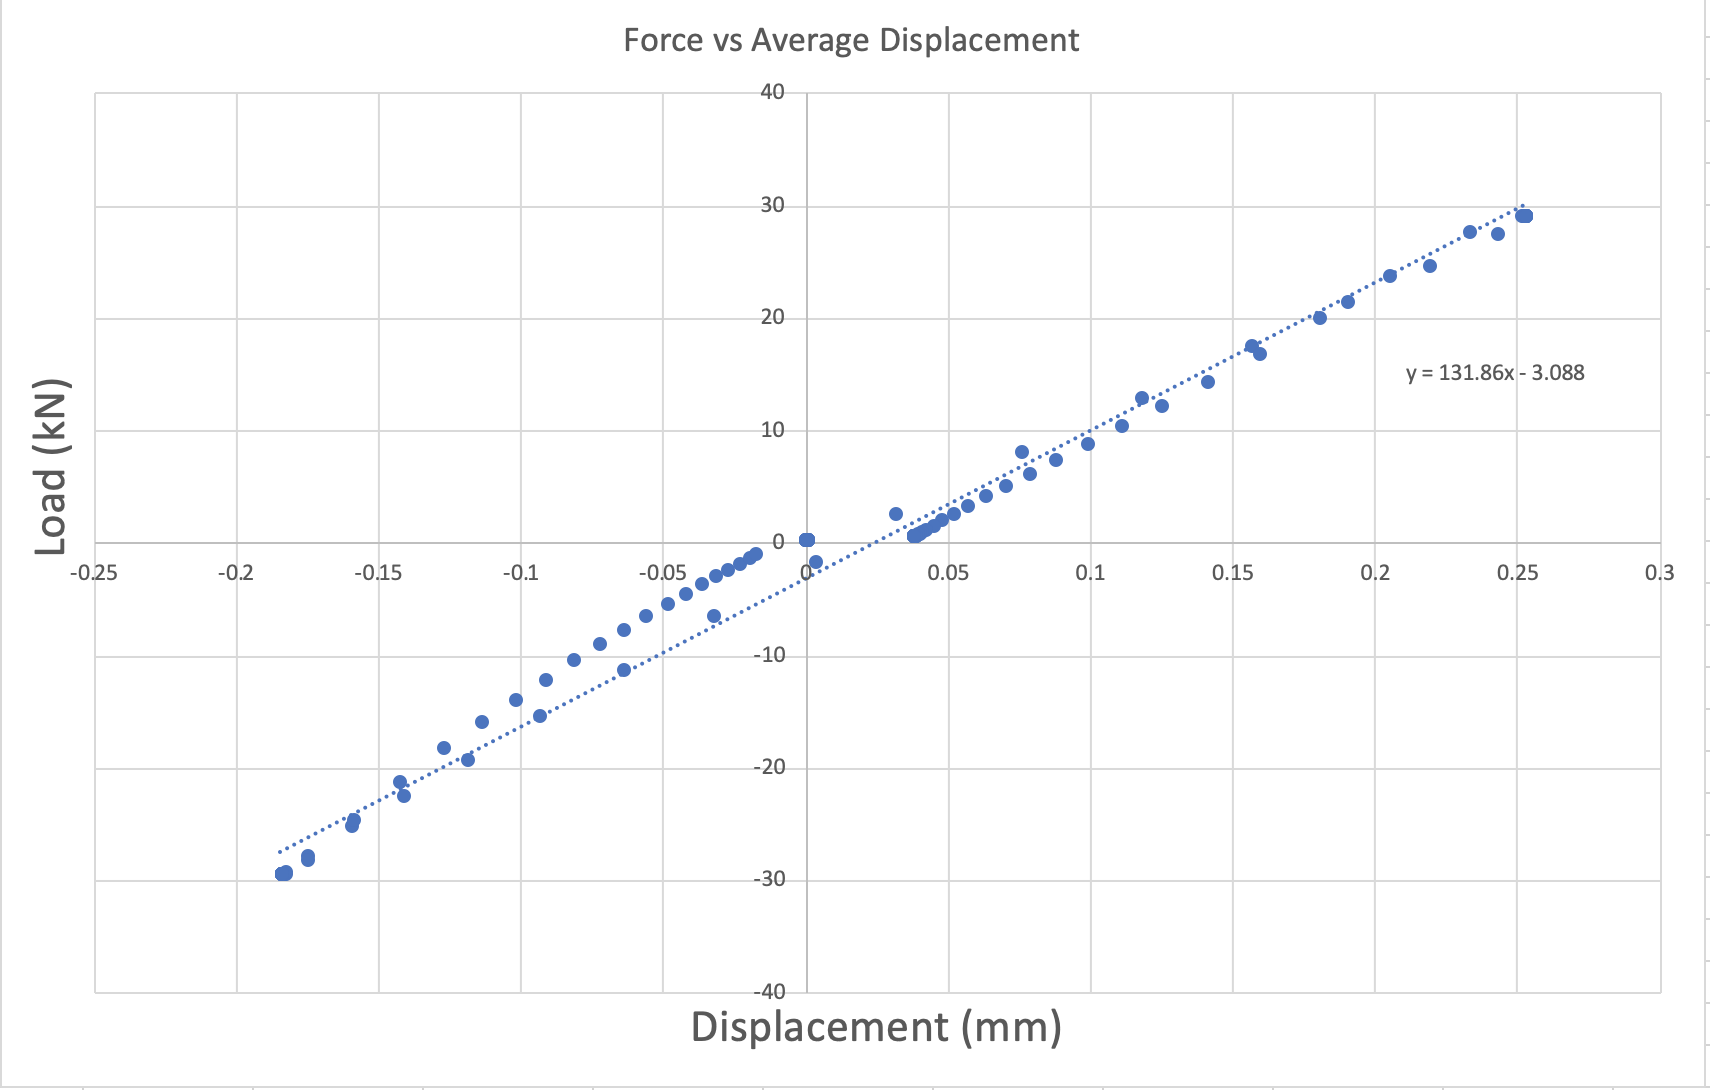
\includegraphics[width=5.98958in]{jira_imgs/4010.png}\\
From this plot, the overall stiffness can be seen to be 131.86kN/mm.

}
\begin{tabular}{p{2cm}p{14cm}}
\toprule
Step 0.9 & Step Execution Status: \textbf{ Pass } \\ \hline
\end{tabular}
 Description \\
{\footnotesize
View the force vs displacement plot in the Labview.

}
\hdashrule[0.5ex]{\textwidth}{1pt}{3mm}
  Expected Result \\
{\footnotesize
The expected actuator stiffness is \textgreater{}= 134 N/um at center
stroke.~\\[2\baselineskip]

}
\hdashrule[0.5ex]{\textwidth}{1pt}{3mm}
  Actual Result \\
{\footnotesize
The following plot was created in Excel using the exported values from
LabView:\\
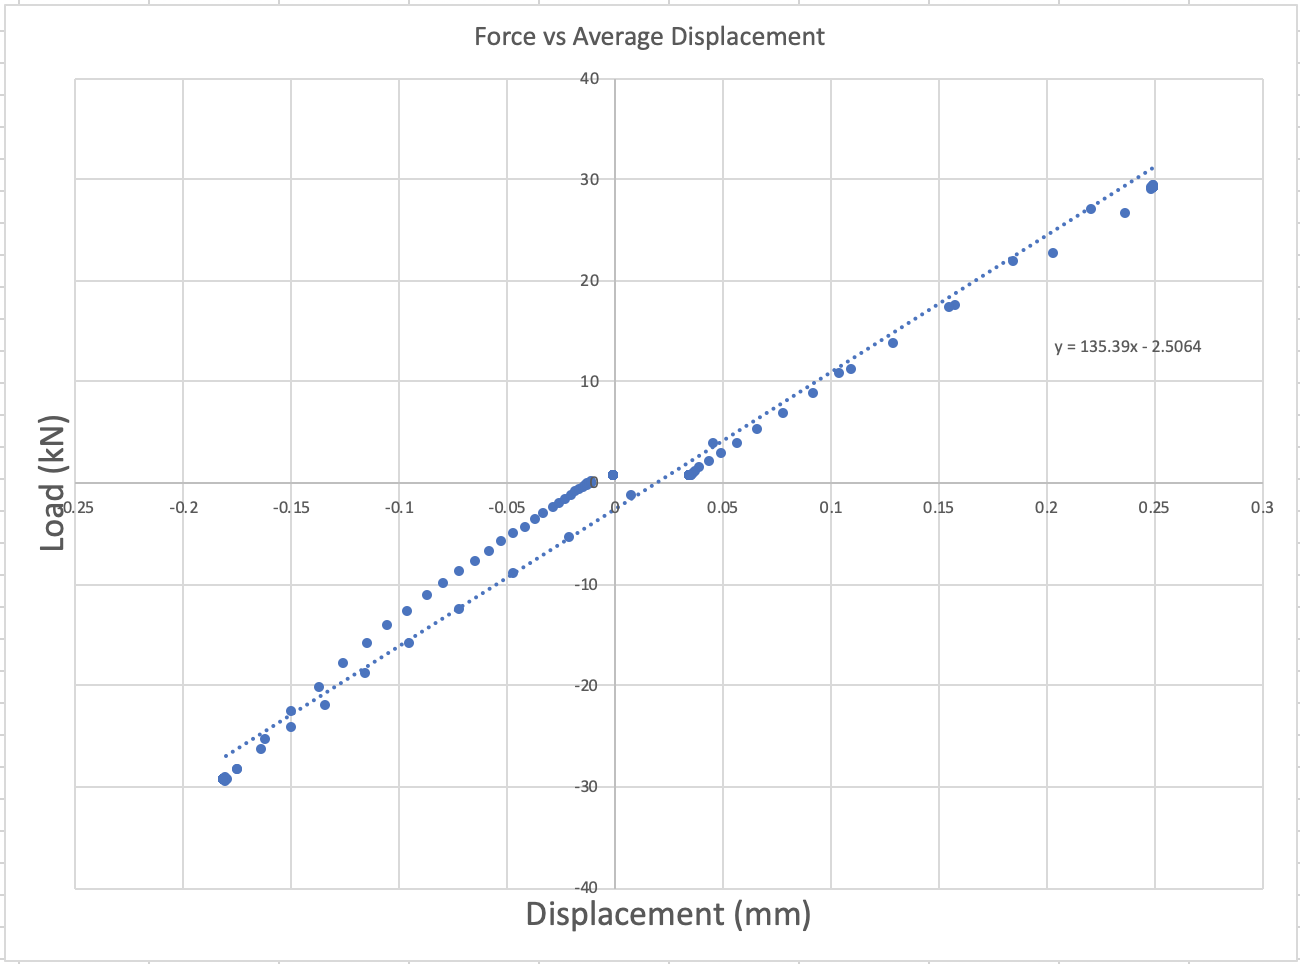
\includegraphics[width=5.98958in]{jira_imgs/4011.png}\\
From this plot, the overall stiffness can be seen to be 135.39kN/mm.

}
\begin{tabular}{p{2cm}p{14cm}}
\toprule
Step 1.1 & Step Execution Status: \textbf{ Pass } \\ \hline
\end{tabular}
 Description \\
{\footnotesize
Open Labview 2021 in the computer used for Test Setup.

}
\hdashrule[0.5ex]{\textwidth}{1pt}{3mm}
  Test Data \\
 {\footnotesize
\textbf{Note:~}The first three steps are conditional because these steps
are included as part of the Test Setup procedure and may not be
necessary if LabView is still open.

}
\hdashrule[0.5ex]{\textwidth}{1pt}{3mm}
  Expected Result \\
{\footnotesize
Labview 2021 opens successfully.

}
\hdashrule[0.5ex]{\textwidth}{1pt}{3mm}
  Actual Result \\
{\footnotesize
LabView and the required VI's were already opened at the start of the
execution of this test cycle.

}
\begin{tabular}{p{2cm}p{14cm}}
\toprule
Step 1.2 & Step Execution Status: \textbf{ Pass } \\ \hline
\end{tabular}
 Description \\
{\footnotesize
Run the following VI's:

\begin{itemize}
\tightlist
\item
  Encoder A (D13B) and Load Cell.vi
\item
  Encoder B (D0BD).vi
\end{itemize}

}
\hdashrule[0.5ex]{\textwidth}{1pt}{3mm}
  Expected Result \\
{\footnotesize
Front panel of VI's open without any error.

}
\hdashrule[0.5ex]{\textwidth}{1pt}{3mm}
  Actual Result \\
{\footnotesize
LabView and the required VI's were already opened at the start of the
execution of this test cycle.

}
\begin{tabular}{p{2cm}p{14cm}}
\toprule
Step 1.3 & Step Execution Status: \textbf{ Pass } \\ \hline
\end{tabular}
 Description \\
{\footnotesize
Click Run button on the block diagram toolbar of the Labview VI front
panel.

}
\hdashrule[0.5ex]{\textwidth}{1pt}{3mm}
  Expected Result \\
{\footnotesize
LabView VI and associated sub Vi runs successfully. The graphs should
start to be populated with data once the run button is pressed.~

}
\hdashrule[0.5ex]{\textwidth}{1pt}{3mm}
  Actual Result \\
{\footnotesize
LabView was ran without any issue.

}
\begin{tabular}{p{2cm}p{14cm}}
\toprule
Step 2.0 & Step Execution Status: \textbf{ Pass } \\ \hline
\end{tabular}
 Description \\
{\footnotesize
Check if all the test results are recorded in excel spreadsheets.

}
\hdashrule[0.5ex]{\textwidth}{1pt}{3mm}
  Expected Result \\
{\footnotesize
Test Results are recorded in the excel spreadsheets residing in the
LabView Folder directory.

}
\hdashrule[0.5ex]{\textwidth}{1pt}{3mm}
  Actual Result \\
{\footnotesize
The results of this test can be found in the Zero Position (unmodified)
sheet of the \emph{Stiffness Test Results Modified vs
Unmodified.xlsx~}document.

}
\begin{tabular}{p{2cm}p{14cm}}
\toprule
Step 2.1 & Step Execution Status: \textbf{ Not Executed } \\ \hline
\end{tabular}
 Description \\
{\footnotesize
Close all the Labview VI files.

}
\hdashrule[0.5ex]{\textwidth}{1pt}{3mm}
  Test Data \\
 {\footnotesize
\textbf{Note:~}Labview can be left open in order to continue to the next
test. However, it may be necessary to reset the application before
starting the next test.

}
\hdashrule[0.5ex]{\textwidth}{1pt}{3mm}
  Expected Result \\
{\footnotesize
All the VI files are closed and Labview 2021 application window closes.

}
\hdashrule[0.5ex]{\textwidth}{1pt}{3mm}
  Actual Result \\
{\footnotesize
The VI's were not closed in order to run through a second iteration of
this test, but the E-stop was reset in order to position the actuator
for the next test iteration.

}
\begin{tabular}{p{2cm}p{14cm}}
\toprule
Step 2.1 & Step Execution Status: \textbf{ Pass } \\ \hline
\end{tabular}
 Description \\
{\footnotesize
Open Labview 2021 in the computer used for Test Setup.

}
\hdashrule[0.5ex]{\textwidth}{1pt}{3mm}
  Test Data \\
 {\footnotesize
\textbf{Note:~}The first three steps are conditional because these steps
are included as part of the Test Setup procedure and may not be
necessary if LabView is still open.

}
\hdashrule[0.5ex]{\textwidth}{1pt}{3mm}
  Expected Result \\
{\footnotesize
Labview 2021 opens successfully.

}
\hdashrule[0.5ex]{\textwidth}{1pt}{3mm}
  Actual Result \\
{\footnotesize
Labview was already open from the first iteration of this test case.

}
\begin{tabular}{p{2cm}p{14cm}}
\toprule
Step 2.2 & Step Execution Status: \textbf{ Pass } \\ \hline
\end{tabular}
 Description \\
{\footnotesize
Run the following VI's:

\begin{itemize}
\tightlist
\item
  Encoder A (D13B) and Load Cell.vi
\item
  Encoder B (D0BD).vi
\end{itemize}

}
\hdashrule[0.5ex]{\textwidth}{1pt}{3mm}
  Expected Result \\
{\footnotesize
Front panel of VI's open without any error.

}
\hdashrule[0.5ex]{\textwidth}{1pt}{3mm}
  Actual Result \\
{\footnotesize
The VI's were already open.

}
\begin{tabular}{p{2cm}p{14cm}}
\toprule
Step 2.3 & Step Execution Status: \textbf{ Pass } \\ \hline
\end{tabular}
 Description \\
{\footnotesize
Click Run button on the block diagram toolbar of the Labview VI front
panel.

}
\hdashrule[0.5ex]{\textwidth}{1pt}{3mm}
  Expected Result \\
{\footnotesize
LabView VI and associated sub Vi runs successfully. The graphs should
start to be populated with data once the run button is pressed.~

}
\hdashrule[0.5ex]{\textwidth}{1pt}{3mm}
  Actual Result \\
{\footnotesize
The VI's were already running. However, the data on the graphs were
cleared in order to export a fresh set of data.

}
\begin{tabular}{p{2cm}p{14cm}}
\toprule
Step 3.0 & Step Execution Status: \textbf{ Pass } \\ \hline
\end{tabular}
 Description \\
{\footnotesize
Check if all the test results are recorded in excel spreadsheets.

}
\hdashrule[0.5ex]{\textwidth}{1pt}{3mm}
  Expected Result \\
{\footnotesize
Test Results are recorded in the excel spreadsheets residing in the
LabView Folder directory.

}
\hdashrule[0.5ex]{\textwidth}{1pt}{3mm}
  Actual Result \\
{\footnotesize
The results of this test can be found in the Positive Limit~(unmodified)
sheet of the \emph{Stiffness Test Results Modified vs
Unmodified.xlsx~}document.

}
\begin{tabular}{p{2cm}p{14cm}}
\toprule
Step 3.1 & Step Execution Status: \textbf{ Not Executed } \\ \hline
\end{tabular}
 Description \\
{\footnotesize
Close all the Labview VI files.

}
\hdashrule[0.5ex]{\textwidth}{1pt}{3mm}
  Test Data \\
 {\footnotesize
\textbf{Note:~}Labview can be left open in order to continue to the next
test. However, it may be necessary to reset the application before
starting the next test.

}
\hdashrule[0.5ex]{\textwidth}{1pt}{3mm}
  Expected Result \\
{\footnotesize
All the VI files are closed and Labview 2021 application window closes.

}
\hdashrule[0.5ex]{\textwidth}{1pt}{3mm}
  Actual Result \\
{\footnotesize
The VI's were not closed in order to run through a second iteration of
this test, but the E-stop was reset in order to position the actuator
for the next test iteration.

}
\begin{tabular}{p{2cm}p{14cm}}
\toprule
Step 3.1 & Step Execution Status: \textbf{ Pass } \\ \hline
\end{tabular}
 Description \\
{\footnotesize
Open Labview 2021 in the computer used for Test Setup.

}
\hdashrule[0.5ex]{\textwidth}{1pt}{3mm}
  Test Data \\
 {\footnotesize
\textbf{Note:~}The first three steps are conditional because these steps
are included as part of the Test Setup procedure and may not be
necessary if LabView is still open.

}
\hdashrule[0.5ex]{\textwidth}{1pt}{3mm}
  Expected Result \\
{\footnotesize
Labview 2021 opens successfully.

}
\hdashrule[0.5ex]{\textwidth}{1pt}{3mm}
  Actual Result \\
{\footnotesize
LabView was already open from the first iteration of this test case.

}
\begin{tabular}{p{2cm}p{14cm}}
\toprule
Step 3.2 & Step Execution Status: \textbf{ Pass } \\ \hline
\end{tabular}
 Description \\
{\footnotesize
Run the following VI's:

\begin{itemize}
\tightlist
\item
  Encoder A (D13B) and Load Cell.vi
\item
  Encoder B (D0BD).vi
\end{itemize}

}
\hdashrule[0.5ex]{\textwidth}{1pt}{3mm}
  Expected Result \\
{\footnotesize
Front panel of VI's open without any error.

}
\hdashrule[0.5ex]{\textwidth}{1pt}{3mm}
  Actual Result \\
{\footnotesize
The VI's were already open.

}
\begin{tabular}{p{2cm}p{14cm}}
\toprule
Step 3.3 & Step Execution Status: \textbf{ Pass } \\ \hline
\end{tabular}
 Description \\
{\footnotesize
Click Run button on the block diagram toolbar of the Labview VI front
panel.

}
\hdashrule[0.5ex]{\textwidth}{1pt}{3mm}
  Expected Result \\
{\footnotesize
LabView VI and associated sub Vi runs successfully. The graphs should
start to be populated with data once the run button is pressed.~

}
\hdashrule[0.5ex]{\textwidth}{1pt}{3mm}
  Actual Result \\
{\footnotesize
The VI's were already running. However, the data on the graphs were
cleared in order to export a fresh set of data.

}
\begin{tabular}{p{2cm}p{14cm}}
\toprule
Step 3.4 & Step Execution Status: \textbf{ Pass } \\ \hline
\end{tabular}
 Description \\
{\footnotesize
Note the starting position read by the encoders, while fully
{retracted}⁠ .

}
\hdashrule[0.5ex]{\textwidth}{1pt}{3mm}
  Test Data \\
 {\footnotesize
\textbf{Note}:\\
Centered = Actuator is at the zero position (Active Load Position =
-40.202mm)\\
Extended = Actuator is at its positive limit switch (Active Load
Position = -25.904mm)\\
Retracted = Actuator is at its negative limit switch (Active Load
Position = -54.501mm)

}
\hdashrule[0.5ex]{\textwidth}{1pt}{3mm}
  Expected Result \\
{\footnotesize
Actuator position confirmed by encoder reading in the
LabView.\\[2\baselineskip]

}
\hdashrule[0.5ex]{\textwidth}{1pt}{3mm}
  Actual Result \\
{\footnotesize
Active Load Position read by Copley = -54.405mm\\[2\baselineskip]As seen
in the ‚ÄãNegative Limit‚Äã‚Äã‚Äã~(unmodified) sheet of the
\emph{Stiffness Test Results Modified vs Unmodified.xlsx~}document, the
starting position measured by the external encoders were as follows:

\begin{itemize}
\tightlist
\item
  Encoder A = 53.9433mm
\item
  Encoder B = 53.5679mm
\end{itemize}

}
\begin{tabular}{p{2cm}p{14cm}}
\toprule
Step 3.5 & Step Execution Status: \textbf{ Pass } \\ \hline
\end{tabular}
 Description \\
{\footnotesize
Disable Motor Power by pressing the Emergency stop button on the control
box.

}
\hdashrule[0.5ex]{\textwidth}{1pt}{3mm}
  Expected Result \\
{\footnotesize
Motor power disabled.

}
\hdashrule[0.5ex]{\textwidth}{1pt}{3mm}
  Actual Result \\
{\footnotesize
The E-stop of the motor was pressed and the control software was seen to
be disabled on the Copley Control.

}
\begin{tabular}{p{2cm}p{14cm}}
\toprule
Step 3.6 & Step Execution Status: \textbf{ Pass } \\ \hline
\end{tabular}
 Description \\
{\footnotesize
While fully {retracted}⁠: Increase the load on the actuator from 0 kN to
approximately +30kN.

}
\hdashrule[0.5ex]{\textwidth}{1pt}{3mm}
  Test Data \\
 {\footnotesize
\textbf{Note:~}To apply +30kN, set Channel 1 = 4.38V and Channel 0 = 0V.

}
\hdashrule[0.5ex]{\textwidth}{1pt}{3mm}
  Expected Result \\
{\footnotesize
Load cell reader shows the applied +30 kN tension force.\\
LabView displays the voltage being applied.

}
\hdashrule[0.5ex]{\textwidth}{1pt}{3mm}
  Actual Result \\
{\footnotesize
Iteration 1:\\
Active Load Position read by Copley = -54.542mm\\
Iteration 2:\\
Active Load Position read by Copley = -54.541mm

}
\begin{tabular}{p{2cm}p{14cm}}
\toprule
Step 3.7 & Step Execution Status: \textbf{ Pass } \\ \hline
\end{tabular}
 Description \\
{\footnotesize
While fully {{retracted}⁠}: Reduce the load to back to 0kN and then to
-30 kN.

}
\hdashrule[0.5ex]{\textwidth}{1pt}{3mm}
  Test Data \\
 {\footnotesize
\textbf{Note:~}To apply -30kN, set Channel 1 = 4.38V and Channel 0 = 0V.

}
\hdashrule[0.5ex]{\textwidth}{1pt}{3mm}
  Expected Result \\
{\footnotesize
Load cell reader shows the applied 0kN force and the -30kN compression
force.

}
\hdashrule[0.5ex]{\textwidth}{1pt}{3mm}
  Actual Result \\
{\footnotesize
Iteration 1:\\
Active Load Position read by Copley = -54.407mm\\
When commanded both compression and tension were reset to zero, the
Active Load Position = -54.401mm\\
Iteration 2:\\
Active Load Position (-30kN) = 54.409mm\\
Active Load Position (0kN) = 54.409mm

}
\begin{tabular}{p{2cm}p{14cm}}
\toprule
Step 3.8 & Step Execution Status: \textbf{ Pass } \\ \hline
\end{tabular}
 Description \\
{\footnotesize
Record the actual displacement as measured by the two external encoders
as LabView graph (Displacement vs Time).\\[2\baselineskip]

}
\hdashrule[0.5ex]{\textwidth}{1pt}{3mm}
  Expected Result \\
{\footnotesize
Actual displacement measured by the average of the two external encoders
~recorded in the LabView graph.

}
\hdashrule[0.5ex]{\textwidth}{1pt}{3mm}
  Actual Result \\
{\footnotesize
The displacement was recorded into a LabView graph (Displacement vs
Time) for each encoder. By right-clicking on the graphs, we were able to
export the values onto an excel file and plot them against displacement.

}
\begin{tabular}{p{2cm}p{14cm}}
\toprule
Step 3.9 & Step Execution Status: \textbf{ Pass } \\ \hline
\end{tabular}
 Description \\
{\footnotesize
View the force vs displacement plot in the Labview.

}
\hdashrule[0.5ex]{\textwidth}{1pt}{3mm}
  Expected Result \\
{\footnotesize
The expected actuator stiffness is \textgreater{}= 134 N/um at center
stroke.~\\[2\baselineskip]

}
\hdashrule[0.5ex]{\textwidth}{1pt}{3mm}
  Actual Result \\
{\footnotesize
The following plot was created in Excel using the exported values from
LabView:\\
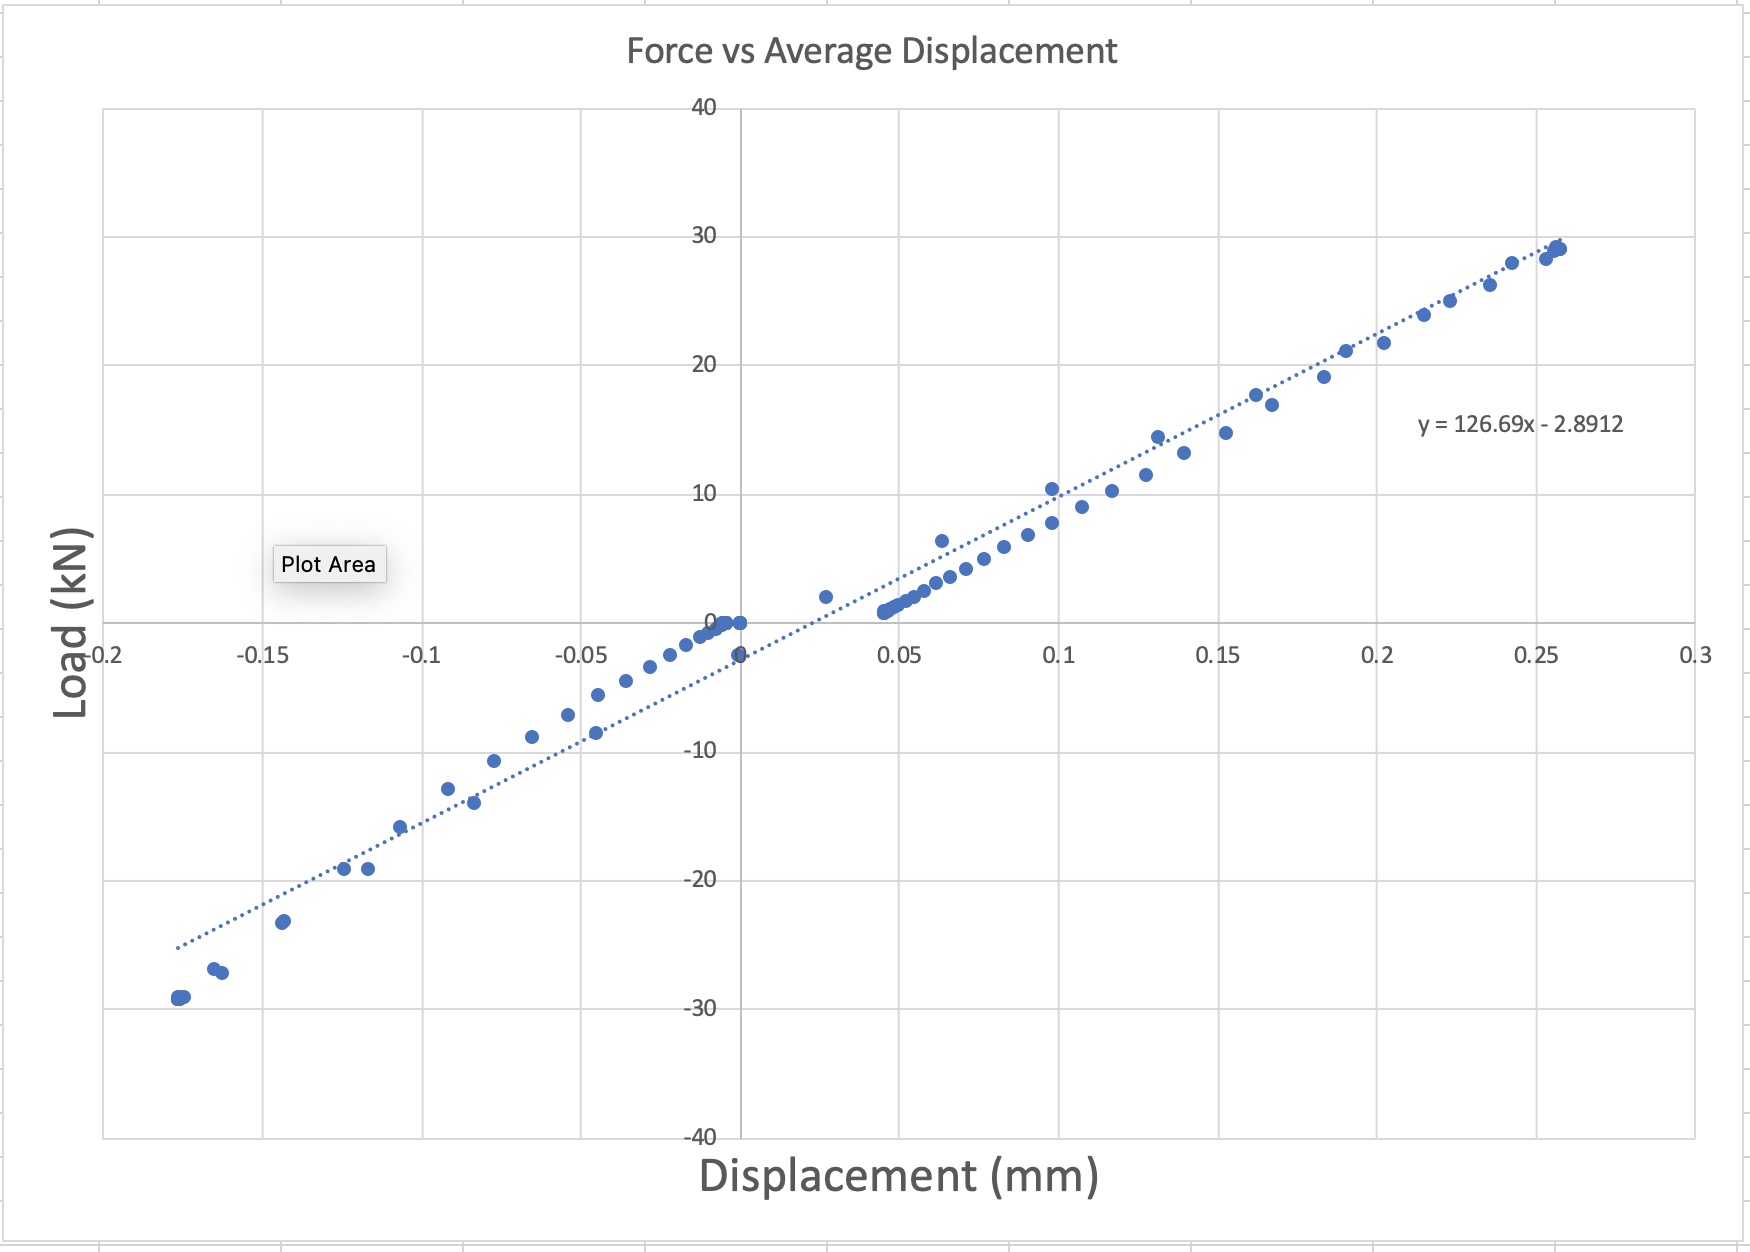
\includegraphics[width=5.98958in]{jira_imgs/4012.png}From this plot, the
overall stiffness can be seen to be 126.69kN/mm.

}
\begin{tabular}{p{2cm}p{14cm}}
\toprule
Step 4.0 & Step Execution Status: \textbf{ Pass } \\ \hline
\end{tabular}
 Description \\
{\footnotesize
Check if all the test results are recorded in excel spreadsheets.

}
\hdashrule[0.5ex]{\textwidth}{1pt}{3mm}
  Expected Result \\
{\footnotesize
Test Results are recorded in the excel spreadsheets residing in the
LabView Folder directory.

}
\hdashrule[0.5ex]{\textwidth}{1pt}{3mm}
  Actual Result \\
{\footnotesize
The results of this test can be found in the Negative~Limit~(unmodified)
sheet of the \emph{Stiffness Test Results Modified vs
Unmodified.xlsx~}document.

}
\begin{tabular}{p{2cm}p{14cm}}
\toprule
Step 4.1 & Step Execution Status: \textbf{ Not Executed } \\ \hline
\end{tabular}
 Description \\
{\footnotesize
Close all the Labview VI files.

}
\hdashrule[0.5ex]{\textwidth}{1pt}{3mm}
  Test Data \\
 {\footnotesize
\textbf{Note:~}Labview can be left open in order to continue to the next
test. However, it may be necessary to reset the application before
starting the next test.

}
\hdashrule[0.5ex]{\textwidth}{1pt}{3mm}
  Expected Result \\
{\footnotesize
All the VI files are closed and Labview 2021 application window closes.

}
\hdashrule[0.5ex]{\textwidth}{1pt}{3mm}
  Actual Result \\
{\footnotesize
The LabView VI's were stopped, but not closed.~

}

\paragraph{ LVV-T2437 - Hexapod - Actuator Movement Test }\mbox{}\\

Version \textbf{1}.
Status \textbf{Approved}.
Open  \href{https://jira.lsstcorp.org/secure/Tests.jspa#/testCase/LVV-T2437}{\textit{ LVV-T2437 } }
test case in Jira.

The purpose of this test will be to verify that the actuators are able
to move within their velocity and acceleration limits. Furthermore,
during the moves, we will also be verifying that the actuators do not
take more than 2 seconds to settle into place.~

\textbf{ Preconditions}:\\


Execution status: {\bf Pass }

Final comment:\\During the test, the velocity and acceleration limits could not be
changed in the Copley control software. However, the limits were already
set to the desired velocity and acceleration. As a result, we verified
that the actuator was still capable of meeting the minimum velocity of
the 0.342mm/s. The settling time was also verified by this test.\\
According to MOOG's original procedure, the settling time started when
the actuator had reached its commanded position of +/-5mm and ended when
the displacement was within 0.001mm of that commanded position. As seen
in the results of this test case, the settling time was always seen to
be less than 2 seconds. This is supported by the raw data as seen in the
\href{https://docushare.lsst.org/docushare/dsweb/Services/Document-55090}{\emph{Movement
Test Results - Unmodified Actuator.xlsx}}\emph{~}document.


Detailed steps results:

\begin{tabular}{p{2cm}p{14cm}}
\toprule
Step 1 & Step Execution Status: \textbf{ Pass } \\ \hline
\end{tabular}
 Description \\
{\footnotesize
Open Labview 2021 in the computer used for Test Setup.

}
\hdashrule[0.5ex]{\textwidth}{1pt}{3mm}
  Test Data \\
 {\footnotesize
The first three steps are conditional because these steps are included
as part of the Test Setup procedure and may not be necessary if LabView
is still open.

}
\hdashrule[0.5ex]{\textwidth}{1pt}{3mm}
  Expected Result \\
{\footnotesize
Labview 2021 opens successfully.

}
\hdashrule[0.5ex]{\textwidth}{1pt}{3mm}
  Actual Result \\
{\footnotesize
LabView and the required VI's were already opened at the start of the
execution of this test cycle.

}
\begin{tabular}{p{2cm}p{14cm}}
\toprule
Step 2 & Step Execution Status: \textbf{ Pass } \\ \hline
\end{tabular}
 Description \\
{\footnotesize
Run the following VI's:

\begin{itemize}
\tightlist
\item
  Encoder A (D13B) and Load Cell.vi
\item
  Encoder B (D0BD).vi
\end{itemize}

}
\hdashrule[0.5ex]{\textwidth}{1pt}{3mm}
  Expected Result \\
{\footnotesize
Front panel of VI's open without any error.

}
\hdashrule[0.5ex]{\textwidth}{1pt}{3mm}
  Actual Result \\
{\footnotesize
LabView and the required VI's were already opened at the start of the
execution of this test cycle.

}
\begin{tabular}{p{2cm}p{14cm}}
\toprule
Step 3 & Step Execution Status: \textbf{ Pass } \\ \hline
\end{tabular}
 Description \\
{\footnotesize
Click Run button on the on the block diagram toolbar of the Labview VI
front panel.

}
\hdashrule[0.5ex]{\textwidth}{1pt}{3mm}
  Expected Result \\
{\footnotesize
LabView VI and associated sub Vi runs successfully. The graphs should
start to be populated with data once the run button is pressed.

}
\hdashrule[0.5ex]{\textwidth}{1pt}{3mm}
  Actual Result \\
{\footnotesize
LabView was ran without any issue.

}
\begin{tabular}{p{2cm}p{14cm}}
\toprule
Step 4 & Step Execution Status: \textbf{ Pass } \\ \hline
\end{tabular}
 Description \\
{\footnotesize
Apply a -15kN compression load by using the LabView function to increase
the air supply value of 2.19V to the compression valve.

}
\hdashrule[0.5ex]{\textwidth}{1pt}{3mm}
  Test Data \\
 {\footnotesize


}
\hdashrule[0.5ex]{\textwidth}{1pt}{3mm}
  Expected Result \\
{\footnotesize
The LabView load graph (Load vs Time) shows -15 KN compression load
applied.

}
\hdashrule[0.5ex]{\textwidth}{1pt}{3mm}
  Actual Result \\
{\footnotesize
Setting the compression valve to 2.19V applied a -15kN force

}
\begin{tabular}{p{2cm}p{14cm}}
\toprule
Step 5 & Step Execution Status: \textbf{ Pass } \\ \hline
\end{tabular}
 Description \\
{\footnotesize
Within the copley software, set the maximum actuator velocity to +/-0.5
mm/s.

}
\hdashrule[0.5ex]{\textwidth}{1pt}{3mm}
  Expected Result \\
{\footnotesize
The maximum velocity is set to 0.5mm/s.

}
\hdashrule[0.5ex]{\textwidth}{1pt}{3mm}
  Actual Result \\
{\footnotesize
The velocity limit could not be changed but was already set to 0.5mm/s

}
\begin{tabular}{p{2cm}p{14cm}}
\toprule
Step 6 & Step Execution Status: \textbf{ Pass } \\ \hline
\end{tabular}
 Description \\
{\footnotesize
Within the copley software, set the actuator acceleration and
deceleration limits to 0.5mm/s\^{}2.

}
\hdashrule[0.5ex]{\textwidth}{1pt}{3mm}
  Expected Result \\
{\footnotesize
The maximum acceleration is set to 0.5mm/s\^{}2.

}
\hdashrule[0.5ex]{\textwidth}{1pt}{3mm}
  Actual Result \\
{\footnotesize
The acceleration and deceleration limits could not be changed but were
already set to 0.5mm/s\^{}s

}
\begin{tabular}{p{2cm}p{14cm}}
\toprule
Step 7 & Step Execution Status: \textbf{ Pass } \\ \hline
\end{tabular}
 Description \\
{\footnotesize
Using the copley software, command the actuator to move relatively +5mm.

}
\hdashrule[0.5ex]{\textwidth}{1pt}{3mm}
  Expected Result \\
{\footnotesize
The Labview graph (Position vs Time) shows the actuator travels 0.342mm
in 2 seconds or less.

}
\hdashrule[0.5ex]{\textwidth}{1pt}{3mm}
  Actual Result \\
{\footnotesize
The displacement was monitored by looking at the (Position vs Time)
graph in Labview. The results were exported onto an excel sheet and
copied below.\\
Before the move:

\begin{itemize}
\tightlist
\item
  Encoder A = 39.63mm
\item
  Encoder B = 39.25mm~
\end{itemize}

After the move:

\begin{itemize}
\tightlist
\item
  Encoder A = 34.65mm
\item
  Encoder B = 34.26mm
\end{itemize}

As seen in the test data on the Compression sheet of the \emph{Movement
Test Results - Unmodified Actuator.xlsx} document, the overall move of
+5mm took about 12 seconds. Therefore, it can be seen that actuator was
traveling at about 0.416mm/s

}
\begin{tabular}{p{2cm}p{14cm}}
\toprule
Step 8 & Step Execution Status: \textbf{ Pass } \\ \hline
\end{tabular}
 Description \\
{\footnotesize
Verify the actuator does not move after reaching the commanded position
by checking the Labview graph (Position vs. Time).

}
\hdashrule[0.5ex]{\textwidth}{1pt}{3mm}
  Expected Result \\
{\footnotesize
The labview graph(Position vs Time) shows the actuator is no longer in
motion.

}
\hdashrule[0.5ex]{\textwidth}{1pt}{3mm}
  Actual Result \\
{\footnotesize
It can roughly be seen from the following plot that there was no
movement after the actuator had reached its commanded position.\\
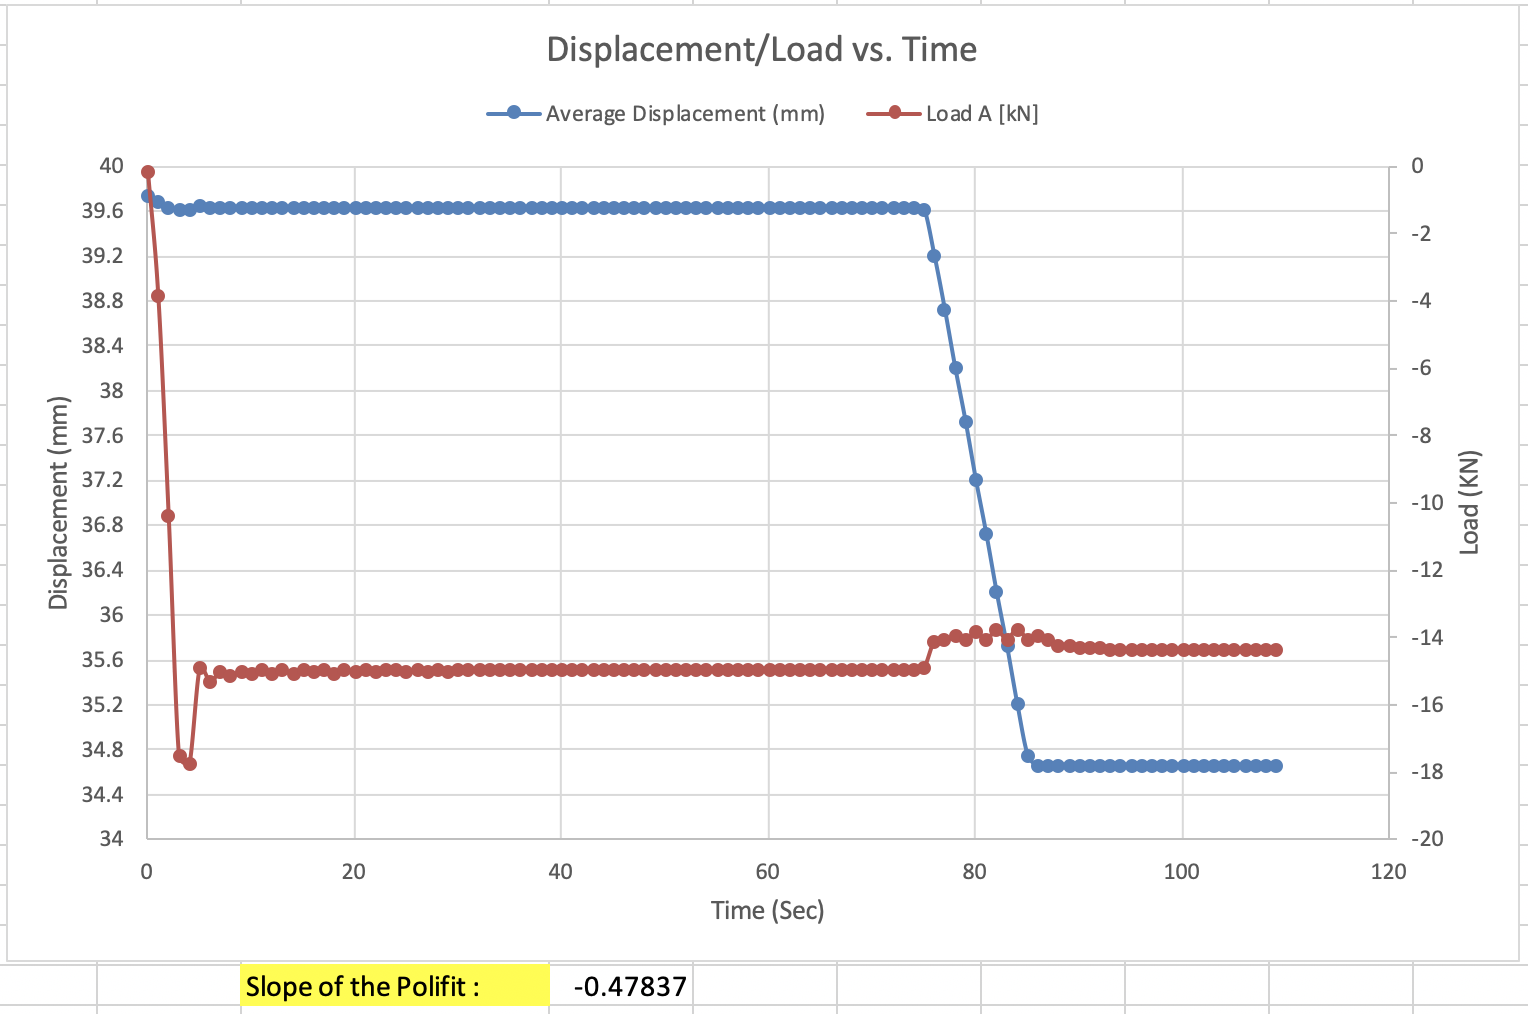
\includegraphics[width=5.98958in]{jira_imgs/4013.png}\\[2\baselineskip]The
test results were recorded in the Compression sheet of the
\emph{Movement Test Results - Unmodified Actuator.xlsx} document. After
Encoder A reached 34.652mm and Encoder B reached 34.261mm, it took about
1 second for the actuator to settle to within 0.001mm of that position.
In 1 second, Encoder A was seen to be at 34.651mm and Encoder B was
34.260mm.

}
\begin{tabular}{p{2cm}p{14cm}}
\toprule
Step 9 & Step Execution Status: \textbf{ Pass } \\ \hline
\end{tabular}
 Description \\
{\footnotesize
Using the copley software, command the actuator to move -5mm
(relatively), returning the original position.

}
\hdashrule[0.5ex]{\textwidth}{1pt}{3mm}
  Test Data \\
 {\footnotesize
\textbf{Note:~}Since the velocity or acceleration limits have not
changed, this should take the same amount of time.

}
\hdashrule[0.5ex]{\textwidth}{1pt}{3mm}
  Expected Result \\
{\footnotesize
The labview graph (Position vs Time) shows the actuator moves back 5mm
in less than 2 seconds.

}
\hdashrule[0.5ex]{\textwidth}{1pt}{3mm}
  Actual Result \\
{\footnotesize
The Copley control software was used to command the actuator back to its
starting position and this was verified by checking the value recorded
by the graph being displayed in LabView. This was confirmed by reading
the values reported by the graph displayed by LabView.

}
\begin{tabular}{p{2cm}p{14cm}}
\toprule
Step 10 & Step Execution Status: \textbf{ Pass } \\ \hline
\end{tabular}
 Description \\
{\footnotesize
Now apply a +15kN tension load by using the LabView function to increase
the air supply value of 2.19V to the tension valve.

}
\hdashrule[0.5ex]{\textwidth}{1pt}{3mm}
  Expected Result \\
{\footnotesize
The LabView load graph (Load vs Time) shows +15 KN tension load has been
applied.

}
\hdashrule[0.5ex]{\textwidth}{1pt}{3mm}
  Actual Result \\
{\footnotesize
The tension valve was set to 2.19V resulting in an application of
+14.89kN load.

}
\begin{tabular}{p{2cm}p{14cm}}
\toprule
Step 11 & Step Execution Status: \textbf{ Pass } \\ \hline
\end{tabular}
 Description \\
{\footnotesize
Using the copley software, command the actuator to move relatively +5mm.

}
\hdashrule[0.5ex]{\textwidth}{1pt}{3mm}
  Expected Result \\
{\footnotesize
The Labview graph (Position vs Time) shows the actuator travels 0.342mm
in 2 seconds or less.

}
\hdashrule[0.5ex]{\textwidth}{1pt}{3mm}
  Actual Result \\
{\footnotesize
The displacement was monitored by looking at the (Position vs Time)
graph in Labview. The results were exported onto an excel sheet and
copied below.\\
Before the move:

\begin{itemize}
\tightlist
\item
  Encoder A = 39.74mm
\item
  Encoder B = 39.36mm~
\end{itemize}

After the move:

\begin{itemize}
\tightlist
\item
  Encoder A = 34.81mm
\item
  Encoder B = 34.40mm
\end{itemize}

As seen in the test data on the Tension sheet of the \emph{Movement Test
Results - Unmodified Actuator.xlsx} document, the overall move of +5mm
took about 9 seconds. Therefore, it can be seen that actuator was
traveling 0.555mm/s.

}
\begin{tabular}{p{2cm}p{14cm}}
\toprule
Step 12 & Step Execution Status: \textbf{ Pass } \\ \hline
\end{tabular}
 Description \\
{\footnotesize
Using the copley software, command the actuator to move -5mm
(relatively), returning the original position.

}
\hdashrule[0.5ex]{\textwidth}{1pt}{3mm}
  Test Data \\
 {\footnotesize
\textbf{Note:~}Since the velocity or acceleration limits have not
changed, this should take the same amount of time.

}
\hdashrule[0.5ex]{\textwidth}{1pt}{3mm}
  Expected Result \\
{\footnotesize
The labview graph (Position vs Time) shows the actuator moves back 5mm
in less than 2 seconds.

}
\hdashrule[0.5ex]{\textwidth}{1pt}{3mm}
  Actual Result \\
{\footnotesize
The displacement was monitored by looking at the (Position vs Time)
graph in LabView and was confirmed that the actuator reached its
original position.

}
\begin{tabular}{p{2cm}p{14cm}}
\toprule
Step 13 & Step Execution Status: \textbf{ Pass } \\ \hline
\end{tabular}
 Description \\
{\footnotesize
Verify the actuator does not move after reaching the commanded position
by checking the Labview graph (Position vs Time).

}
\hdashrule[0.5ex]{\textwidth}{1pt}{3mm}
  Expected Result \\
{\footnotesize
The labview graph (Position vs Time) shows the actuator is no longer in
motion.

}
\hdashrule[0.5ex]{\textwidth}{1pt}{3mm}
  Actual Result \\
{\footnotesize
It can roughly be seen from the following plot that there was no
movement after the actuator had reached its commanded position.\\
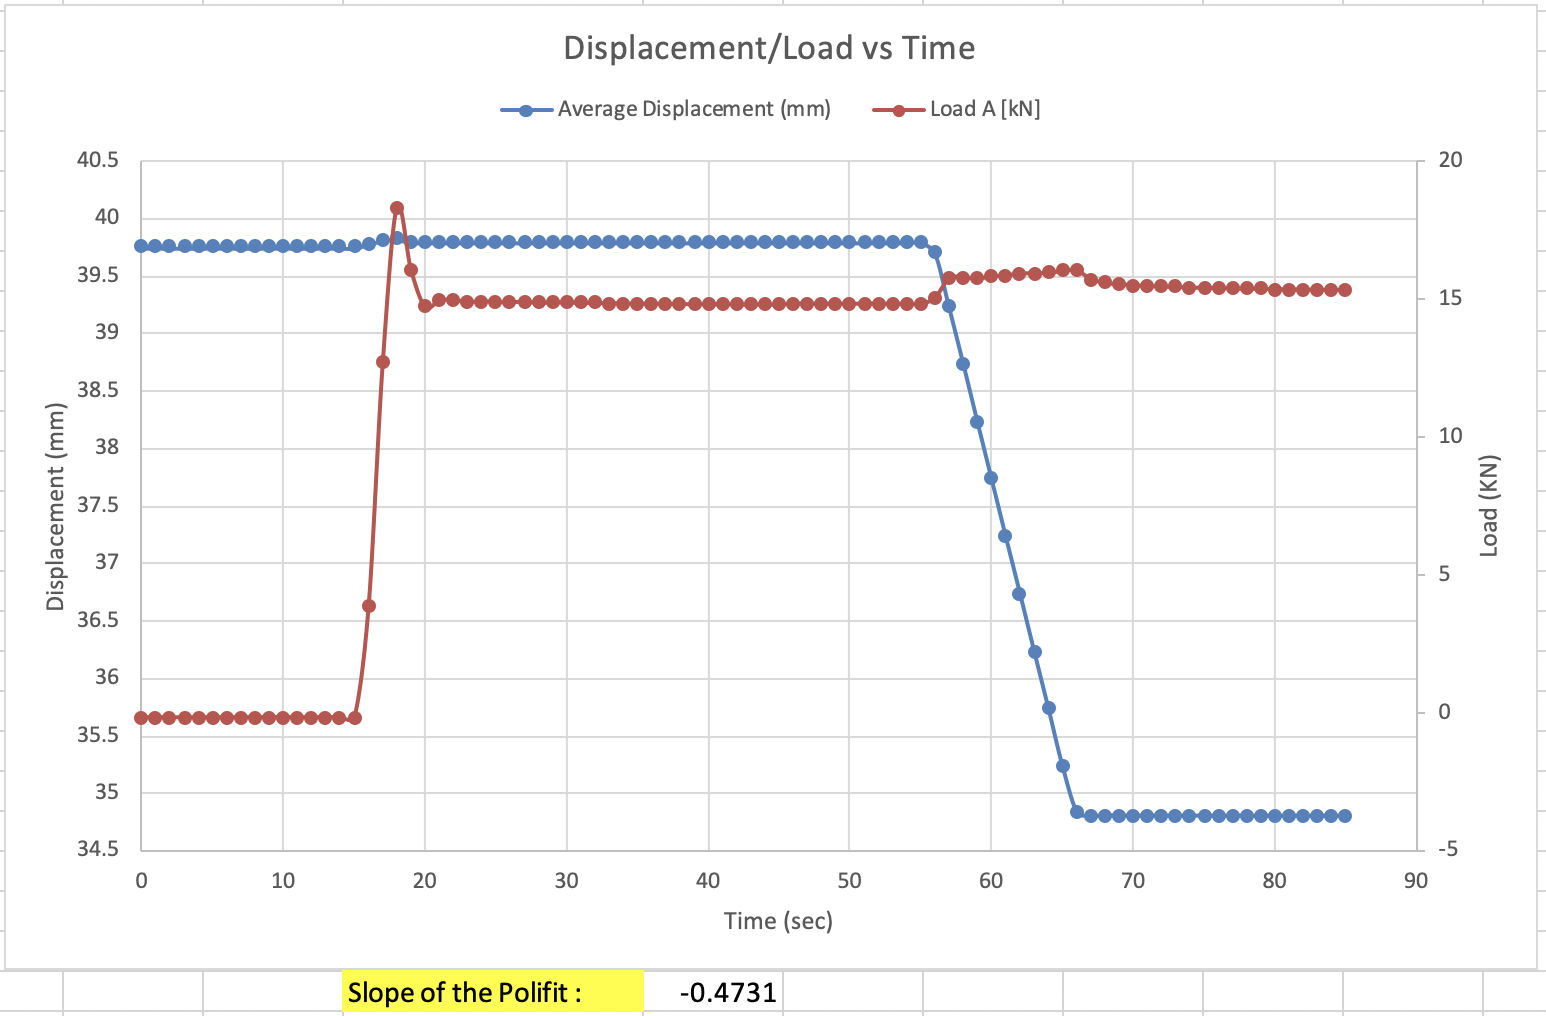
\includegraphics[width=5.98958in]{jira_imgs/4014.png}\\
The test results were recorded in the Tension sheet of the
\emph{Movement Test Results - Unmodified Actuator.xlsx} document.After
Encoder A reached 34.814mm and Encoder B reached 34.408mm, it took about
1 second for the actuator to settle to within 0.001mm of that position.
In 1 second, Encoder A was seen to be 34.814mm and Encoder B was
34.408mm.

}
\begin{tabular}{p{2cm}p{14cm}}
\toprule
Step 14 & Step Execution Status: \textbf{ Pass } \\ \hline
\end{tabular}
 Description \\
{\footnotesize
Check if all the test results are recorded in excel spreadsheets.

}
\hdashrule[0.5ex]{\textwidth}{1pt}{3mm}
  Expected Result \\
{\footnotesize
Test Results are recorded in the excel spreadsheets residing in the
LabView Folder directory.

}
\hdashrule[0.5ex]{\textwidth}{1pt}{3mm}
  Actual Result \\
{\footnotesize
The test results were recorded in the \emph{Movement Test Results -
Unmodified Actuator.xlsx} document.

}
\begin{tabular}{p{2cm}p{14cm}}
\toprule
Step 15 & Step Execution Status: \textbf{ Not Executed } \\ \hline
\end{tabular}
 Description \\
{\footnotesize
Close all the Labview VI files.

}
\hdashrule[0.5ex]{\textwidth}{1pt}{3mm}
  Test Data \\
 {\footnotesize
\textbf{Note:~}Labview can be left open in order to continue to the next
test. However, it may be necessary to reset the application before
starting the next test.

}
\hdashrule[0.5ex]{\textwidth}{1pt}{3mm}
  Expected Result \\
{\footnotesize
All the VI files are closed and Labview 2021 application window closes.

}
\hdashrule[0.5ex]{\textwidth}{1pt}{3mm}
  Actual Result \\
{\footnotesize
The LabView VI's were stopped, but not closed.~

}

\paragraph{ LVV-T2432 - Hexapod - Actuator Range of Motion Test }\mbox{}\\

Version \textbf{1}.
Status \textbf{Approved}.
Open  \href{https://jira.lsstcorp.org/secure/Tests.jspa#/testCase/LVV-T2432}{\textit{ LVV-T2432 } }
test case in Jira.

To verify that the range of motions for the actuators stay within the
determined limits.

\textbf{ Preconditions}:\\
The range limits should be determined to achieve the camera hexapod's
simultaneous range of motion requirements.

Execution status: {\bf Pass }

Final comment:\\The original scope of this test was to verify the position of the
positive and negative limit switches using the Copley Control software.
There were additional steps involved based on MOOG's original procedure
that cited that the software limit switches would be set and needed to
be adjusted in order to do so. However, MOOG used additional software to
set and adjust the software limit switches of the actuator. Therefore,
those steps were skipped for the purposes of this test and only the
steps related to determining the physical limit switches were tested.~


Detailed steps results:

\begin{tabular}{p{2cm}p{14cm}}
\toprule
Step 1 & Step Execution Status: \textbf{ Pass } \\ \hline
\end{tabular}
 Description \\
{\footnotesize
Open Labview 2021 in the computer used for Test Setup.

}
\hdashrule[0.5ex]{\textwidth}{1pt}{3mm}
  Test Data \\
 {\footnotesize
The first three steps are conditional because these steps are included
as part of the Test Setup procedure and may not be necessary if LabView
is still open.\\[3\baselineskip]

}
\hdashrule[0.5ex]{\textwidth}{1pt}{3mm}
  Expected Result \\
{\footnotesize
Labview 2021 opens successfully.

}
\hdashrule[0.5ex]{\textwidth}{1pt}{3mm}
  Actual Result \\
{\footnotesize
LabView and the required VI's were already opened at the start of the
execution of this test cycle.

}
\begin{tabular}{p{2cm}p{14cm}}
\toprule
Step 2 & Step Execution Status: \textbf{ Pass } \\ \hline
\end{tabular}
 Description \\
{\footnotesize
Run the following VI's:

\begin{itemize}
\tightlist
\item
  Encoder A (D13B) and Load Cell.vi
\item
  Encoder B (D0BD).vi
\end{itemize}

}
\hdashrule[0.5ex]{\textwidth}{1pt}{3mm}
  Expected Result \\
{\footnotesize
Front panel of the VI's open without any error.

}
\hdashrule[0.5ex]{\textwidth}{1pt}{3mm}
  Actual Result \\
{\footnotesize
LabView and the required VI's were already opened at the start of the
execution of this test cycle.

}
\begin{tabular}{p{2cm}p{14cm}}
\toprule
Step 3 & Step Execution Status: \textbf{ Pass } \\ \hline
\end{tabular}
 Description \\
{\footnotesize
Click Run button on the block diagram toolbar of the Labview VI front
panel.

}
\hdashrule[0.5ex]{\textwidth}{1pt}{3mm}
  Expected Result \\
{\footnotesize
LabView VI and associated sub Vi runs successfully. The graphs should
start to be populated with data once the run button is pressed.

}
\hdashrule[0.5ex]{\textwidth}{1pt}{3mm}
  Actual Result \\
{\footnotesize
LabView was ran without any issue.

}
\begin{tabular}{p{2cm}p{14cm}}
\toprule
Step 4 & Step Execution Status: \textbf{ Fail } \\ \hline
\end{tabular}
 Description \\
{\footnotesize
Set software actuator stroke limits using the copley software to +/-
14.00mm.

}
\hdashrule[0.5ex]{\textwidth}{1pt}{3mm}
  Expected Result \\
{\footnotesize
Software actuator stroke limits set to +/- 14.00mm.

}
\hdashrule[0.5ex]{\textwidth}{1pt}{3mm}
  Actual Result \\
{\footnotesize
From the initial validation of the limit switches (See
\href{https://jira.lsstcorp.org/secure/Tests.jspa\#/testPlayer/testExecution/LVV-E2735}{LVV-E2735}),
we determined the limit switches to be at +/-14.298mm from the absolute
zero position. However, we were unable to set the software actuator
stroke limits.~

}
\begin{tabular}{p{2cm}p{14cm}}
\toprule
Step 5 & Step Execution Status: \textbf{ Pass } \\ \hline
\end{tabular}
 Description \\
{\footnotesize
Move the actuator forward and backward to confirm that positive position
commands correspond to extensions of the actuator and negative position
commands correspond to retractions of the actuator. If not, flipped the
sign of the encoder readings in software.~\\[2\baselineskip]

}
\hdashrule[0.5ex]{\textwidth}{1pt}{3mm}
  Expected Result \\
{\footnotesize
Positive position commands correspond to extensions; Negative position
commands correspond to retractions of the actuator.~

}
\hdashrule[0.5ex]{\textwidth}{1pt}{3mm}
  Actual Result \\
{\footnotesize
During the execution of the Hexapod - Actuator Test Set Up (See
\href{https://jira.lsstcorp.org/secure/Tests.jspa\#/testPlayer/testExecution/LVV-E2735}{LVV-E2735}),
we were able observe that the actuator position became increasingly more
positive as the actuator was extended until it tripped the positive
limit switch. The same was determined when the actuator position became
increasingly negative as the actuator retracted until it tripped the
negative limit switch.\\[2\baselineskip]Furthermore, during the
execution for the Actuator Back Driving Test
(See~\href{https://jira.lsstcorp.org/secure/Tests.jspa\#/testPlayer/testExecution/LVV-E2738}{LVV-E2738}),
we confirmed that applying a tension force (+kN) resulted in a more
positive actuator position (extension) while applying a compression
force (-kN) resulted in a more negative actuator position (retraction).

}
\begin{tabular}{p{2cm}p{14cm}}
\toprule
Step 6 & Step Execution Status: \textbf{ Pass } \\ \hline
\end{tabular}
 Description \\
{\footnotesize
Set the motor drive to halt motion using the control box and copley
software if a limit switch is tripped.\\[3\baselineskip]

}
\hdashrule[0.5ex]{\textwidth}{1pt}{3mm}
  Expected Result \\
{\footnotesize
Motor drive set to halt position if a limit switch is tripped.~

}
\hdashrule[0.5ex]{\textwidth}{1pt}{3mm}
  Actual Result \\
{\footnotesize
The actuator was confirmed to stop once it tripped a limit switch. The
software would display the fault and no motion could be commanded
further into the limit switch.

}
\begin{tabular}{p{2cm}p{14cm}}
\toprule
Step 7 & Step Execution Status: \textbf{ Fail } \\ \hline
\end{tabular}
 Description \\
{\footnotesize
Extend the actuator to its position stroke limit of +14mm using the
copley software and the~ control box.

}
\hdashrule[0.5ex]{\textwidth}{1pt}{3mm}
  Expected Result \\
{\footnotesize
Actuator extended to its position stroke limit of +14mm.

}
\hdashrule[0.5ex]{\textwidth}{1pt}{3mm}
  Actual Result \\
{\footnotesize
During MOOG's original testing, they used a separate software that
allowed them to set/change the software limits of the actuator. Instead,
the position of the limit switches were simply verified without setting
the software limits. Since the software limits were not set, this step
is marked as Fail.~

}
\begin{tabular}{p{2cm}p{14cm}}
\toprule
Step 8 & Step Execution Status: \textbf{ Not Executed } \\ \hline
\end{tabular}
 Description \\
{\footnotesize
Ensure that the actuator reaches this position without hitting the
mechanical end stop or extension limit switch.

}
\hdashrule[0.5ex]{\textwidth}{1pt}{3mm}
  Expected Result \\
{\footnotesize
Encoder reading in LabView shows that actuator reached the position.~\\
Mechanical End Stop/Extension Limit switch not hit.

}
\hdashrule[0.5ex]{\textwidth}{1pt}{3mm}
  Actual Result \\
{\footnotesize
As mentioned in the previous step, since the software limits of the
actuator could not be set/changed, this step was not executed.~

}
\begin{tabular}{p{2cm}p{14cm}}
\toprule
Step 9 & Step Execution Status: \textbf{ Not Executed } \\ \hline
\end{tabular}
 Description \\
{\footnotesize
If the extension limit switch is contacted, the extension limit switch
position will need to be adjusted to be greater than 14mm and then the
try to extend the actuator to the position stroke limit of +14mm using
copley software and the control box.

}
\hdashrule[0.5ex]{\textwidth}{1pt}{3mm}
  Expected Result \\
{\footnotesize
Extension Limit Switch position readjusted and extended to the position
stroke limit of +14mm.

}
\hdashrule[0.5ex]{\textwidth}{1pt}{3mm}
  Actual Result \\
{\footnotesize
Again, since the software limits of the actuator could not be
set/changed, this step was not executed. Furthermore, this step was
conditional.

}
\begin{tabular}{p{2cm}p{14cm}}
\toprule
Step 10 & Step Execution Status: \textbf{ Not Executed } \\ \hline
\end{tabular}
 Description \\
{\footnotesize
Ensure that the actuator reaches this position without hitting the
mechanical end stop or extension limit switch.

}
\hdashrule[0.5ex]{\textwidth}{1pt}{3mm}
  Expected Result \\
{\footnotesize
Encoder reading in LabView shows that actuator reached the position.\\
Mechanical End Stop/Extension Limit switch not hit.

}
\hdashrule[0.5ex]{\textwidth}{1pt}{3mm}
  Actual Result \\
{\footnotesize
Again, since the software limits of the actuator could not be
set/changed, this step was not executed. Furthermore, this step was
conditional.

}
\begin{tabular}{p{2cm}p{14cm}}
\toprule
Step 11 & Step Execution Status: \textbf{ Not Executed } \\ \hline
\end{tabular}
 Description \\
{\footnotesize
Move the extension actuator stroke limit using the copley software to
+15.00mm .

}
\hdashrule[0.5ex]{\textwidth}{1pt}{3mm}
  Expected Result \\
{\footnotesize
Extension actuator stroke limit moved to +15.00mm.~

}
\hdashrule[0.5ex]{\textwidth}{1pt}{3mm}
  Actual Result \\
{\footnotesize
As mentioned in the previous step, since the software limits of the
actuator could not be set/changed, this step was not executed.

}
\begin{tabular}{p{2cm}p{14cm}}
\toprule
Step 12 & Step Execution Status: \textbf{ Pass } \\ \hline
\end{tabular}
 Description \\
{\footnotesize
Extend the actuator at maximum velocity until the extension limit switch
is actuated.

}
\hdashrule[0.5ex]{\textwidth}{1pt}{3mm}
  Test Data \\
 {\footnotesize
\textbf{Note:~}The maximum velocity is +/-0.5mm/s

}
\hdashrule[0.5ex]{\textwidth}{1pt}{3mm}
  Expected Result \\
{\footnotesize
Actuator extended at maximum velocity until the extension limit switch
is actuated.~

}
\hdashrule[0.5ex]{\textwidth}{1pt}{3mm}
  Actual Result \\
{\footnotesize
The maximum velocity on the Copley control software was set to 0.5mm/s
by default. The actuator was commanded to about +14mm initially and then
in increments of +0.1mm until the limit switch was triggered. As a
result, the limit switch was seen to be triggered at +14.298mm.

}
\begin{tabular}{p{2cm}p{14cm}}
\toprule
Step 13 & Step Execution Status: \textbf{ Not Executed } \\ \hline
\end{tabular}
 Description \\
{\footnotesize
If the actuator hits the stroke limit before tripping the limit switch
or appears to contact the end stop after tripping the limit switch
(before it can stop), reposition the limit switch. Then, repeat test
using copley software and the control box.\\[2\baselineskip]

}
\hdashrule[0.5ex]{\textwidth}{1pt}{3mm}
  Expected Result \\
{\footnotesize
Limit switch repositioned and extended the actuator to the position
stroke limit of +15mm.~

}
\hdashrule[0.5ex]{\textwidth}{1pt}{3mm}
  Actual Result \\
{\footnotesize
During MOOG's original testing, they used a separate software that
allowed them to set the stroke limits of the actuator. Instead, the
position of the limit switches were simply verified without using
software limits. Since this does not impact the results of our tests,
this step was skipped.

}
\begin{tabular}{p{2cm}p{14cm}}
\toprule
Step 14 & Step Execution Status: \textbf{ Pass } \\ \hline
\end{tabular}
 Description \\
{\footnotesize
Record the final position of the limit switch.~\\[2\baselineskip]

}
\hdashrule[0.5ex]{\textwidth}{1pt}{3mm}
  Expected Result \\
{\footnotesize
Final position of the limit switch is around +14.50mm.

}
\hdashrule[0.5ex]{\textwidth}{1pt}{3mm}
  Actual Result \\
{\footnotesize
The limit switch position was seen to be +14.298mm as recorded in the
execution of the Actuator Test Set up (See
\href{https://jira.lsstcorp.org/secure/Tests.jspa\#/testPlayer/testExecution/LVV-E2735}{LVV-E2735}).

}
\begin{tabular}{p{2cm}p{14cm}}
\toprule
Step 15 & Step Execution Status: \textbf{ Not Executed } \\ \hline
\end{tabular}
 Description \\
{\footnotesize
Repeat the steps 6-14 two more times to assess limit switch position
repeatability. ~\\[3\baselineskip]

}
\hdashrule[0.5ex]{\textwidth}{1pt}{3mm}
  Expected Result \\
{\footnotesize
Final positions of the limit switch close to step 14 result(Around
+14.50).

}
\hdashrule[0.5ex]{\textwidth}{1pt}{3mm}
  Actual Result \\
{\footnotesize
The limit switch was seen to be roughly around +14.298mm as recorded in
step 14 when repeated once more. However, this step was skipped as we
didn't want to cause hysteresis in the paddle for the limit switch.

}
\begin{tabular}{p{2cm}p{14cm}}
\toprule
Step 16 & Step Execution Status: \textbf{ Fail } \\ \hline
\end{tabular}
 Description \\
{\footnotesize
Retract the actuator to its position stroke limit of -14 mm using the
copley software and the ~control box.\\[2\baselineskip]

}
\hdashrule[0.5ex]{\textwidth}{1pt}{3mm}
  Expected Result \\
{\footnotesize
Actuator retracted to its position stroke limit of -14.04mm.

}
\hdashrule[0.5ex]{\textwidth}{1pt}{3mm}
  Actual Result \\
{\footnotesize
During MOOG's original testing, they used a separate software that
allowed them to set/change the software limits of the actuator. Instead,
the position of the limit switches were simply verified without setting
the software limits. Since the software limits were not set, this step
is marked as Fail.

}
\begin{tabular}{p{2cm}p{14cm}}
\toprule
Step 17 & Step Execution Status: \textbf{ Not Executed } \\ \hline
\end{tabular}
 Description \\
{\footnotesize
Ensure that the actuator reaches this position without hitting the
mechanical end stop or retraction limit switch.

}
\hdashrule[0.5ex]{\textwidth}{1pt}{3mm}
  Expected Result \\
{\footnotesize
Encoder reading in LabView shows that actuator reached the position.\\
Mechanical End Stop/Retraction Limit switch not hit.

}
\hdashrule[0.5ex]{\textwidth}{1pt}{3mm}
  Actual Result \\
{\footnotesize
As mentioned in the previous step, since the software limits of the
actuator could not be set/changed, this step was not executed.

}
\begin{tabular}{p{2cm}p{14cm}}
\toprule
Step 18 & Step Execution Status: \textbf{ Not Executed } \\ \hline
\end{tabular}
 Description \\
{\footnotesize
If the retraction limit switch is contacted, the retraction limit switch
position will need to be adjusted to be greater than -14mm and then the
try to retract the actuator to the position stroke limit of -14mm using
copley software and the control box.

}
\hdashrule[0.5ex]{\textwidth}{1pt}{3mm}
  Expected Result \\
{\footnotesize
Retraction limit switch position readjusted and the actuator retracted
to the position stroke limit of -14mm.

}
\hdashrule[0.5ex]{\textwidth}{1pt}{3mm}
  Actual Result \\
{\footnotesize
Again, since the software limits of the actuator could not be
set/changed, this step was not executed. Furthermore, this step was
conditional.

}
\begin{tabular}{p{2cm}p{14cm}}
\toprule
Step 19 & Step Execution Status: \textbf{ Not Executed } \\ \hline
\end{tabular}
 Description \\
{\footnotesize
Ensure that the actuator reaches this position without hitting the
mechanical end stop or retraction limit switch.

}
\hdashrule[0.5ex]{\textwidth}{1pt}{3mm}
  Expected Result \\
{\footnotesize
Encoder reading in LabView shows that actuator reached the position.\\
Mechanical End Stop/Retraction Limit switch not hit.

}
\hdashrule[0.5ex]{\textwidth}{1pt}{3mm}
  Actual Result \\
{\footnotesize
Again, since the software limits of the actuator could not be
set/changed, this step was not executed. Furthermore, this step was
conditional.

}
\begin{tabular}{p{2cm}p{14cm}}
\toprule
Step 20 & Step Execution Status: \textbf{ Not Executed } \\ \hline
\end{tabular}
 Description \\
{\footnotesize
Move the retraction actuator stroke limit to -15.00mm .~

}
\hdashrule[0.5ex]{\textwidth}{1pt}{3mm}
  Expected Result \\
{\footnotesize
Retraction actuator stroke limit moved to -15.00mm.

}
\hdashrule[0.5ex]{\textwidth}{1pt}{3mm}
  Actual Result \\
{\footnotesize
As mentioned in the previous step, since the software limits of the
actuator could not be set/changed, this step was not executed.

}
\begin{tabular}{p{2cm}p{14cm}}
\toprule
Step 21 & Step Execution Status: \textbf{ Pass } \\ \hline
\end{tabular}
 Description \\
{\footnotesize
Retract the actuator at maximum velocity until the retraction limit
switch is actuated.

}
\hdashrule[0.5ex]{\textwidth}{1pt}{3mm}
  Test Data \\
 {\footnotesize
\textbf{Note:~}The maximum velocity is +/-0.5mm/s

}
\hdashrule[0.5ex]{\textwidth}{1pt}{3mm}
  Expected Result \\
{\footnotesize
Actuator retracted at maximum velocity until the retraction limit switch
is actuated.

}
\hdashrule[0.5ex]{\textwidth}{1pt}{3mm}
  Actual Result \\
{\footnotesize
The maximum velocity on the Copley control software was set to 0.5mm/s
by default. The actuator was commanded to about -14mm initially and then
in increments of -0.1mm until the limit switch was triggered. As a
result, the limit switch was seen to be triggered at -14.298mm.

}
\begin{tabular}{p{2cm}p{14cm}}
\toprule
Step 22 & Step Execution Status: \textbf{ Not Executed } \\ \hline
\end{tabular}
 Description \\
{\footnotesize
If the actuator hits the stroke limit before tripping the limit switch
or appears to contact the end stop after tripping the limit switch
(before it can stop), reposition the limit switch and repeat test.

}
\hdashrule[0.5ex]{\textwidth}{1pt}{3mm}
  Expected Result \\
{\footnotesize
Limit switch repositioned and retracted the actuator to the position
stroke limit of -15mm.

}
\hdashrule[0.5ex]{\textwidth}{1pt}{3mm}
  Actual Result \\
{\footnotesize
During MOOG's original testing, they used a separate software that
allowed them to set the software limits of the actuator. Instead, the
position of the limit switches were simply verified without using
software limits. Since this does not impact the results of our tests,
this step was skipped.

}
\begin{tabular}{p{2cm}p{14cm}}
\toprule
Step 23 & Step Execution Status: \textbf{ Pass } \\ \hline
\end{tabular}
 Description \\
{\footnotesize
Record the final position of the limit switch.

}
\hdashrule[0.5ex]{\textwidth}{1pt}{3mm}
  Expected Result \\
{\footnotesize
Final position of the limit switch is around -14.50mm.

}
\hdashrule[0.5ex]{\textwidth}{1pt}{3mm}
  Actual Result \\
{\footnotesize
The limit switch position was seen to be -14.298mm as recorded in the
execution of the Actuator Test Set up (See
\href{https://jira.lsstcorp.org/secure/Tests.jspa\#/testPlayer/testExecution/LVV-E2735}{LVV-E2735}).

}
\begin{tabular}{p{2cm}p{14cm}}
\toprule
Step 24 & Step Execution Status: \textbf{ Not Executed } \\ \hline
\end{tabular}
 Description \\
{\footnotesize
Repeat the steps 16-23 two more times to assess limit switch position
repeatability.

}
\hdashrule[0.5ex]{\textwidth}{1pt}{3mm}
  Expected Result \\
{\footnotesize
Final positions of the limit switch close to step 15 result(Around
-14.50).

}
\hdashrule[0.5ex]{\textwidth}{1pt}{3mm}
  Actual Result \\
{\footnotesize
The limit switch was seen to be roughly around -14.298mm as recorded in
step 23 when repeated once more. However, this step was skipped as we
didn't want to cause hysteresis in the paddle for the limit switch.

}
\begin{tabular}{p{2cm}p{14cm}}
\toprule
Step 25 & Step Execution Status: \textbf{ Pass } \\ \hline
\end{tabular}
 Description \\
{\footnotesize
Check if all the test results are recorded in excel spreadsheets.

}
\hdashrule[0.5ex]{\textwidth}{1pt}{3mm}
  Expected Result \\
{\footnotesize
Test Results are recorded in the excel spreadsheets residing in the
LabView Folder directory.\\[2\baselineskip]

}
\hdashrule[0.5ex]{\textwidth}{1pt}{3mm}
  Actual Result \\
{\footnotesize
The positions as measured by the External encoders were exported from
LabView and collected into the \emph{Positive and Negative Limit Switch
Readings.xlsx~}document. It can be seen in this results document that
the average position of the encoders was:

\begin{itemize}
\tightlist
\item
  Positive Limit Switch = 25.11mm
\item
  Negative Limit Switch = 54.21mm
\end{itemize}

}
\begin{tabular}{p{2cm}p{14cm}}
\toprule
Step 26 & Step Execution Status: \textbf{ Not Executed } \\ \hline
\end{tabular}
 Description \\
{\footnotesize
Close the Labview Vi file.

}
\hdashrule[0.5ex]{\textwidth}{1pt}{3mm}
  Test Data \\
 {\footnotesize
\textbf{Note:~}Labview can be left open in order to continue to the next
test. However, it may be necessary to reset the application before
starting the next test.

}
\hdashrule[0.5ex]{\textwidth}{1pt}{3mm}
  Expected Result \\
{\footnotesize
Labview 2021 application window closes.

}
\hdashrule[0.5ex]{\textwidth}{1pt}{3mm}
  Actual Result \\
{\footnotesize
The LabView VI's were stopped, but not closed.

}

\paragraph{ LVV-T2434 - Hexapod - Actuator Resolution Test }\mbox{}\\

Version \textbf{1}.
Status \textbf{Approved}.
Open  \href{https://jira.lsstcorp.org/secure/Tests.jspa#/testCase/LVV-T2434}{\textit{ LVV-T2434 } }
test case in Jira.



\textbf{ Preconditions}:\\
This test can be performed at any starting position within the
actuator's range of motion that allow the test to be completed without
exceeding the software range limits. It is preferable to use different
starting positions for different actuators although no performance
deviations are expected.~\\[2\baselineskip]

Execution status: {\bf Pass }

Final comment:\\The test was performed starting from the zero position (Active Copley =
-40.202mm).\\[2\baselineskip]The expected result of this test was that
given 100nm moves with any load, the actuator would reach the commanded
position within 50nm. However, there were some deviations to the 100nm
moves seen to be greater than 50nm. This was expected as MOOG's original
test results described similar issues related to excessive noise on the
load cell and on the external encoders. Additionally, a load
compensation could not be performed with the displacement being measured
in nm's. Therefore, since the encoders were seen to be able to track the
actuator movement closely and in the correct commanded direction, this
test was passed.


Detailed steps results:

\begin{tabular}{p{2cm}p{14cm}}
\toprule
Step 1 & Step Execution Status: \textbf{ Pass } \\ \hline
\end{tabular}
 Description \\
{\footnotesize
Open Labview 2021 in the computer used for Test Setup.~

}
\hdashrule[0.5ex]{\textwidth}{1pt}{3mm}
  Test Data \\
 {\footnotesize
The first three steps are conditional because these steps are included
as part of the Test Setup procedure and may not be necessary if LabView
is still open.

}
\hdashrule[0.5ex]{\textwidth}{1pt}{3mm}
  Expected Result \\
{\footnotesize
Labview 2021 opens successfully.~

}
\hdashrule[0.5ex]{\textwidth}{1pt}{3mm}
  Actual Result \\
{\footnotesize
LabView and the required VI's were already opened at the start of the
execution of this test cycle.

}
\begin{tabular}{p{2cm}p{14cm}}
\toprule
Step 2 & Step Execution Status: \textbf{ Pass } \\ \hline
\end{tabular}
 Description \\
{\footnotesize
Run the following VI's:

\begin{itemize}
\tightlist
\item
  Encoder A (D13B) and Load Cell.vi
\item
  Encoder B (D0BD).vi
\end{itemize}

}
\hdashrule[0.5ex]{\textwidth}{1pt}{3mm}
  Expected Result \\
{\footnotesize
Front panel of VI's open without any error.

}
\hdashrule[0.5ex]{\textwidth}{1pt}{3mm}
  Actual Result \\
{\footnotesize
LabView and the required VI's were already opened at the start of the
execution of this test cycle.

}
\begin{tabular}{p{2cm}p{14cm}}
\toprule
Step 3 & Step Execution Status: \textbf{ Pass } \\ \hline
\end{tabular}
 Description \\
{\footnotesize
Click Run button on the block diagram toolbar of the Labview VI front
panel.

}
\hdashrule[0.5ex]{\textwidth}{1pt}{3mm}
  Expected Result \\
{\footnotesize
LabView VI and associated sub Vi runs successfully. The graphs should
start to be populated with data once the run button is pressed.

}
\hdashrule[0.5ex]{\textwidth}{1pt}{3mm}
  Actual Result \\
{\footnotesize
LabView was ran without any issue.

}
\begin{tabular}{p{2cm}p{14cm}}
\toprule
Step 4 & Step Execution Status: \textbf{ Pass } \\ \hline
\end{tabular}
 Description \\
{\footnotesize
Apply a force of +15kN.

}
\hdashrule[0.5ex]{\textwidth}{1pt}{3mm}
  Test Data \\
 {\footnotesize
\textbf{Note:~}In order to apply a tension force of +15 kN, set Channel
1 = 2.19V and Channel 0 = 0V.~

}
\hdashrule[0.5ex]{\textwidth}{1pt}{3mm}
  Expected Result \\
{\footnotesize
Load cell reader shows the applied +15 KN \textbf{tension} force.\\
LabView displays the voltage being applied.

}
\hdashrule[0.5ex]{\textwidth}{1pt}{3mm}
  Actual Result \\
{\footnotesize
By setting a 2.19V on the tension valve, a +13.91kN force was applied.

}
\begin{tabular}{p{2cm}p{14cm}}
\toprule
Step 5 & Step Execution Status: \textbf{ Pass } \\ \hline
\end{tabular}
 Description \\
{\footnotesize
Record the load cell value in the LabView in the form of Load vs Time
graph.~

}
\hdashrule[0.5ex]{\textwidth}{1pt}{3mm}
  Expected Result \\
{\footnotesize
LabView load graph (Load vs Time) shows +15 kN tension force applied.~

}
\hdashrule[0.5ex]{\textwidth}{1pt}{3mm}
  Actual Result \\
{\footnotesize
The values measuring the load were exported from LabView into the
Tension sheet of the
\href{https://docushare.lsst.org/docushare/dsweb/Services/Document-55070}{\emph{Resolution
Test Results - Unmodified Actuator.xlsx}}\emph{~}excel document. The
applied load during this test can be seen as the orange line in the plot
below:\\
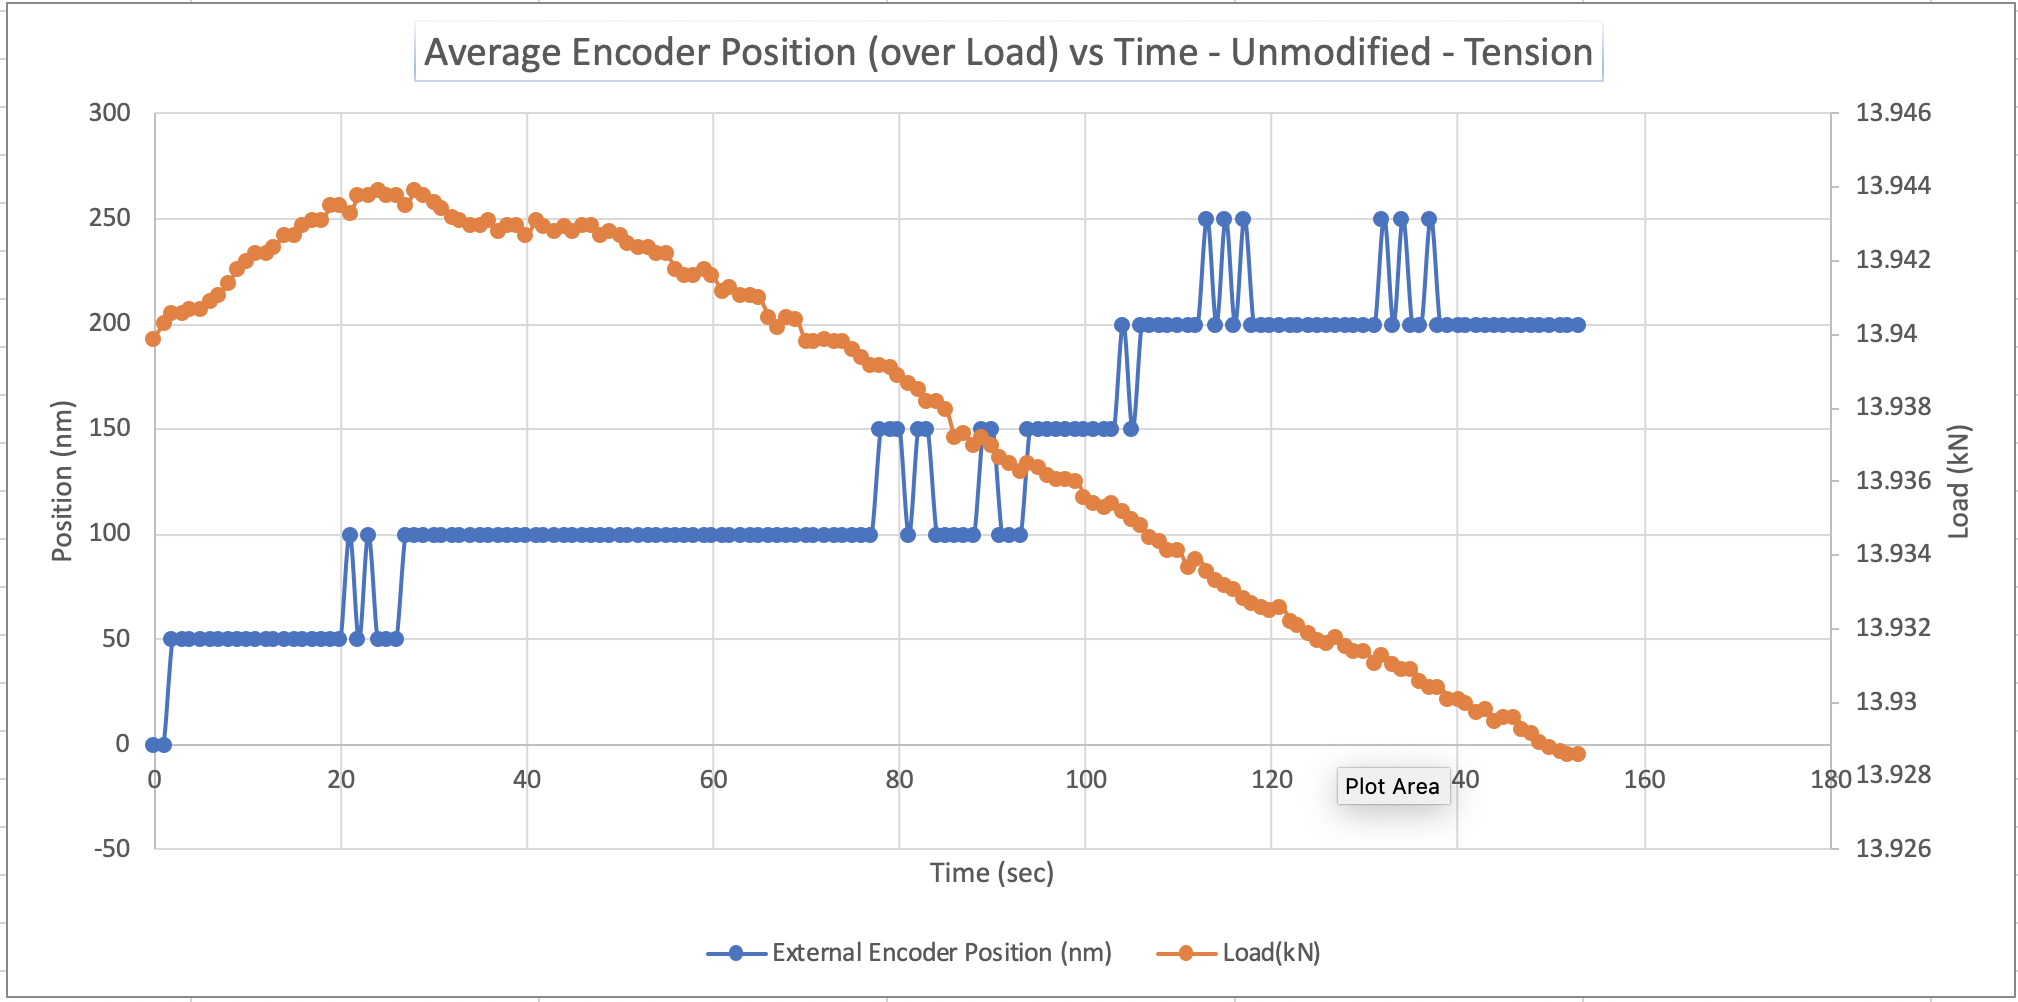
\includegraphics[width=5.98958in]{jira_imgs/4016.png}\\
Note: At the time of this test, the air supply in the testing bay was
being inconsistent and so it was agreed to continue the test at
+13.91kN.

}
\begin{tabular}{p{2cm}p{14cm}}
\toprule
Step 6 & Step Execution Status: \textbf{ Pass } \\ \hline
\end{tabular}
 Description \\
{\footnotesize
Execute the following commands to the actuator in relative positioning
mode using the copley software and the control box : extend 100nm,
extend 100nm, extend 100nm, retract 100nm, extend 100nm, retract 100nm,
retract 100nm, retract 100nm.\\[2\baselineskip]

}
\hdashrule[0.5ex]{\textwidth}{1pt}{3mm}
  Test Data \\
 {\footnotesize
\textbf{Note:~}Take note of the time at which the moves are commanded.
It will be difficult to determine when the series of commands are sent
because the moves are so small.

}
\hdashrule[0.5ex]{\textwidth}{1pt}{3mm}
  Expected Result \\
{\footnotesize
All moves should move in the commanded directions.~

}
\hdashrule[0.5ex]{\textwidth}{1pt}{3mm}
  Actual Result \\
{\footnotesize
Moved +100nm (10:59:54)\\[2\baselineskip]Moved +100nm
(11:00:12)\\[2\baselineskip]Moved +100nm
(11:00:24)\\[2\baselineskip]Moved -100nm
(11:00:33)\\[2\baselineskip]Moved +100nm
(11:00:42)\\[2\baselineskip]Moved -100nm
(11:00:51)\\[2\baselineskip]Moved -100nm
(11:00:58)\\[2\baselineskip]Moved -100nm
(11:01:04)\\[2\baselineskip]These are consistent to the timestamps taken
in the~Tension sheet of the attached \emph{Resolution Test Results -
Unmodified Actuator.xlsx~}excel document

}
\begin{tabular}{p{2cm}p{14cm}}
\toprule
Step 7 & Step Execution Status: \textbf{ Pass } \\ \hline
\end{tabular}
 Description \\
{\footnotesize
Record the actual displacement as measured by the two external encoders
as LabView graph (Displacement vs Time).

}
\hdashrule[0.5ex]{\textwidth}{1pt}{3mm}
  Expected Result \\
{\footnotesize
Actual displacement measured by the average of the two external encoders
~recorded in the LabView graph.~

}
\hdashrule[0.5ex]{\textwidth}{1pt}{3mm}
  Actual Result \\
{\footnotesize
The displacement can be seen as the blue line in the plot attached to
the result of Step 5.

}
\begin{tabular}{p{2cm}p{14cm}}
\toprule
Step 8 & Step Execution Status: \textbf{ Pass } \\ \hline
\end{tabular}
 Description \\
{\footnotesize
Record the actual displacement as measured by the internal encoder using
copley software.~

}
\hdashrule[0.5ex]{\textwidth}{1pt}{3mm}
  Expected Result \\
{\footnotesize
Actual displacement measured by the internal encoder recorded in the
Copley Software.

}
\hdashrule[0.5ex]{\textwidth}{1pt}{3mm}
  Actual Result \\
{\footnotesize
The Active Load Position reported by the Copley Control Software could
not be exported. However, we confirmed after every move that the
relative motion moved +/-100nm each command as reported by the Copley
Control Software.

}
\begin{tabular}{p{2cm}p{14cm}}
\toprule
Step 9 & Step Execution Status: \textbf{ Pass } \\ \hline
\end{tabular}
 Description \\
{\footnotesize
Ensure that the load cell signal did not vary significantly during the
test which would introduce compliance errors.

}
\hdashrule[0.5ex]{\textwidth}{1pt}{3mm}
  Expected Result \\
{\footnotesize
The tension load should remain close to 15kN throughout the displacement
movements and display in the Load vs Time graph in LabView.~

}
\hdashrule[0.5ex]{\textwidth}{1pt}{3mm}
  Actual Result \\
{\footnotesize
As seen in the Tension sheet of the \emph{Resolution Test Results -
Unmodified Actuator.xlsx~}excel document, the load was fairly consistent
at +13.9kN. However, there was still some noise seen that may have
impacted the results of this test. This is similar to what was seen
during MOOG's original test and so this step can still be considered as
passed.

}
\begin{tabular}{p{2cm}p{14cm}}
\toprule
Step 10 & Step Execution Status: \textbf{ Pass } \\ \hline
\end{tabular}
 Description \\
{\footnotesize
Remove the 15 kN tension load.

}
\hdashrule[0.5ex]{\textwidth}{1pt}{3mm}
  Test Data \\
 {\footnotesize
\textbf{Note:~}Set Channel 0 = Channel 1 = 0V.

}
\hdashrule[0.5ex]{\textwidth}{1pt}{3mm}
  Expected Result \\
{\footnotesize
Load cell reader and Load graph in the LabView showing zero
load.\\[2\baselineskip]

}
\hdashrule[0.5ex]{\textwidth}{1pt}{3mm}
  Actual Result \\
{\footnotesize
The tension force was removed

}
\begin{tabular}{p{2cm}p{14cm}}
\toprule
Step 11 & Step Execution Status: \textbf{ Pass } \\ \hline
\end{tabular}
 Description \\
{\footnotesize
Compare the internal linear encoder measurement with the average of the
two external linear encoder measurements.~

}
\hdashrule[0.5ex]{\textwidth}{1pt}{3mm}
  Expected Result \\
{\footnotesize
The magnitude should not vary by more than 50\% from the commanded value
based on an average of the two external linear encoder measurements.

}
\hdashrule[0.5ex]{\textwidth}{1pt}{3mm}
  Actual Result \\
{\footnotesize
The average displacement did not vary by more than 50nm during the
sequence of moves.\\[2\baselineskip]This can be seen in column K of the
Tension sheet in the \emph{Resolution Test Results - Unmodified
Actuator.xlsx~}excel document.

}
\begin{tabular}{p{2cm}p{14cm}}
\toprule
Step 12 & Step Execution Status: \textbf{ Pass } \\ \hline
\end{tabular}
 Description \\
{\footnotesize
Apply a -15kN force.

}
\hdashrule[0.5ex]{\textwidth}{1pt}{3mm}
  Test Data \\
 {\footnotesize
\textbf{Note:~}In order to apply a compression force of -15 kN, set
Channel 0 = 2.19V and Channel 1 = 0V.

}
\hdashrule[0.5ex]{\textwidth}{1pt}{3mm}
  Expected Result \\
{\footnotesize
Load cell reader shows the applied -15 KN \textbf{compression} force.\\
LabView displays the voltage being applied.

}
\hdashrule[0.5ex]{\textwidth}{1pt}{3mm}
  Actual Result \\
{\footnotesize
Setting the voltage of the compression valve to 2.19V yielded a force of
-14.92kN

}
\begin{tabular}{p{2cm}p{14cm}}
\toprule
Step 13 & Step Execution Status: \textbf{ Pass } \\ \hline
\end{tabular}
 Description \\
{\footnotesize
Execute the following commands to the actuator in relative positioning
mode using the copley software and the control box: extend 100nm, extend
100nm, extend 100nm, retract 100nm, extend 100nm, retract 100nm, retract
100nm, retract 100nm.\\[2\baselineskip]

}
\hdashrule[0.5ex]{\textwidth}{1pt}{3mm}
  Test Data \\
 {\footnotesize
\textbf{Note:~}Take note of the time at which the moves are commanded.
It will be difficult to determine when the series of commands are sent
because the moves are so small.

}
\hdashrule[0.5ex]{\textwidth}{1pt}{3mm}
  Expected Result \\
{\footnotesize
All moves should move in the commanded direction.

}
\hdashrule[0.5ex]{\textwidth}{1pt}{3mm}
  Actual Result \\
{\footnotesize
Moved +100nm (11:08:48)\\[2\baselineskip]Moved +100nm
(11:08:54)\\[2\baselineskip]Moved +100nm
(11:09:04)\\[2\baselineskip]Moved -100nm
(11:09:11)\\[2\baselineskip]Moved +100nm
(11:09:20)\\[2\baselineskip]Moved -100nm
(11:09:29)\\[2\baselineskip]Moved -100nm
(11:09:36)\\[2\baselineskip]Moved -100nm
(11:09:43)\\[2\baselineskip]These are consistent to the timestamps taken
in the Compression sheet of the attached \emph{Resolution Test Results -
Unmodified Actuator.xlsx~}excel document

}
\begin{tabular}{p{2cm}p{14cm}}
\toprule
Step 14 & Step Execution Status: \textbf{ Pass } \\ \hline
\end{tabular}
 Description \\
{\footnotesize
Record the actual displacement as measured by average of ~the two
external encoder as Labview graph (Displacement vs. Time).

}
\hdashrule[0.5ex]{\textwidth}{1pt}{3mm}
  Expected Result \\
{\footnotesize
Actual displacement measured by the average of the two external encoders
~recorded in the LabView graph.

}
\hdashrule[0.5ex]{\textwidth}{1pt}{3mm}
  Actual Result \\
{\footnotesize
The values measuring the load were exported from LabView into the
Compression sheet of the \emph{Resolution Test Results - Unmodified
Actuator.xlsx~}excel document.The applied load during this test can be
seen as the orange line in the plot below:\\
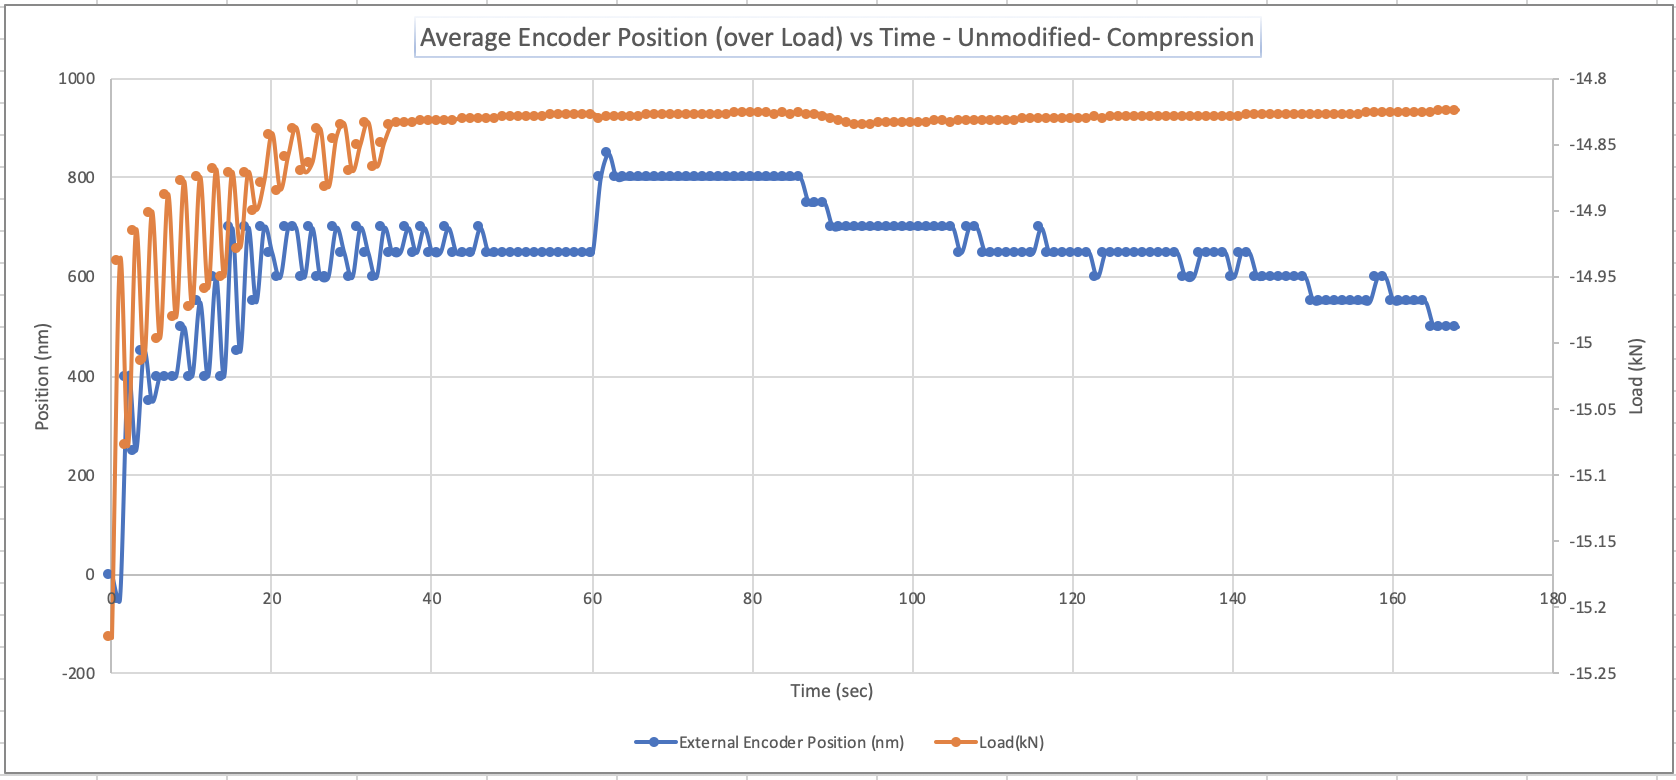
\includegraphics[width=5.98958in]{jira_imgs/4017.png}\\
Note: At the time of this test, the air supply in the testing bay was
being inconsistent and so it was agreed to continue the test at +14.8kN.

}
\begin{tabular}{p{2cm}p{14cm}}
\toprule
Step 15 & Step Execution Status: \textbf{ Pass } \\ \hline
\end{tabular}
 Description \\
{\footnotesize
Record the actual displacement as measured by the internal encoder using
copley software.

}
\hdashrule[0.5ex]{\textwidth}{1pt}{3mm}
  Expected Result \\
{\footnotesize
Actual displacement measured by the internal encoder recorded in the
Copley Software.~

}
\hdashrule[0.5ex]{\textwidth}{1pt}{3mm}
  Actual Result \\
{\footnotesize
The Active Load Position reported by the Copley Control Software could
not be exported. However, we confirmed after every move that the
relative motion moved +/-100nm each command as reported by the Copley
Control Software.

}
\begin{tabular}{p{2cm}p{14cm}}
\toprule
Step 16 & Step Execution Status: \textbf{ Pass } \\ \hline
\end{tabular}
 Description \\
{\footnotesize
Remove the 15 kN compression load.

}
\hdashrule[0.5ex]{\textwidth}{1pt}{3mm}
  Test Data \\
 {\footnotesize
\textbf{Note:~}Set Channel 0 = Channel 1 = 0V.\\[2\baselineskip]

}
\hdashrule[0.5ex]{\textwidth}{1pt}{3mm}
  Expected Result \\
{\footnotesize
Load cell reader and Load graph in the LabView showing zero
load.\\[2\baselineskip]

}
\hdashrule[0.5ex]{\textwidth}{1pt}{3mm}
  Actual Result \\
{\footnotesize
Compression load removed.

}
\begin{tabular}{p{2cm}p{14cm}}
\toprule
Step 17 & Step Execution Status: \textbf{ Pass } \\ \hline
\end{tabular}
 Description \\
{\footnotesize
Compare the internal linear encoder measurement with the average of the
two external linear encoder measurements.

}
\hdashrule[0.5ex]{\textwidth}{1pt}{3mm}
  Expected Result \\
{\footnotesize
Comparison of the Displacement graphs ( External vs internal) in
LabView. The magnitude should not vary by more than 50\% from the
commanded value based on an average of the two external linear encoder
measurements.\\[2\baselineskip]

}
\hdashrule[0.5ex]{\textwidth}{1pt}{3mm}
  Actual Result \\
{\footnotesize
For the unmodified actuator, only the external encoders were tested to
create a baseline to compare the modified actuator results. The average
displacement of the external encoders did not vary by more than 50nm
during the majority of the sequence of moves.\\[2\baselineskip]This can
be seen in column K of the Compression sheet in the \emph{Resolution
Test Results - Unmodified Actuator.xlsx~}excel document. At the time of
the greatest deviations, there were some noise on the load cell that
could have been impacting the results. However, when the load became
steady at 14.82kN, there was only a single deviation seen on Row 63.

}
\begin{tabular}{p{2cm}p{14cm}}
\toprule
Step 18 & Step Execution Status: \textbf{ Pass } \\ \hline
\end{tabular}
 Description \\
{\footnotesize
With Zero load applied to the actuator, execute the following commands
to the actuator in relative positioning mode using the copley software
and the control box: extend 100nm, extend 100nm, extend 100nm, retract
100nm, extend 100nm, retract 100nm, retract 100nm, retract 100nm.

}
\hdashrule[0.5ex]{\textwidth}{1pt}{3mm}
  Test Data \\
 {\footnotesize
\textbf{Note:~}Take note of the time at which the moves are commanded.
It will be difficult to determine when the series of commands are sent
because the moves are so small.

}
\hdashrule[0.5ex]{\textwidth}{1pt}{3mm}
  Expected Result \\
{\footnotesize
All moves should move in the commanded direction.

}
\hdashrule[0.5ex]{\textwidth}{1pt}{3mm}
  Actual Result \\
{\footnotesize
Moved +100nm (11:05:18)\\[2\baselineskip]Moved +100nm
(11:05:27)\\[2\baselineskip]Moved +100nm
(11:05:34)\\[2\baselineskip]Moved -100nm
(11:05:46)\\[2\baselineskip]Moved +100nm
(11:05:54)\\[2\baselineskip]Moved -100nm
(11:06:03)\\[2\baselineskip]Moved -100nm
(11:06:10)\\[2\baselineskip]Moved -100nm
(11:06:16)\\[2\baselineskip]These are consistent to the timestamps taken
in the Zero sheet of the attached \emph{Resolution Test Results -
Unmodified Actuator.xlsx~}excel document

}
\begin{tabular}{p{2cm}p{14cm}}
\toprule
Step 19 & Step Execution Status: \textbf{ Pass } \\ \hline
\end{tabular}
 Description \\
{\footnotesize
Record the actual displacement as measured by average of ~the two
external encoder as Labview graph (Displacement vs Time).

}
\hdashrule[0.5ex]{\textwidth}{1pt}{3mm}
  Expected Result \\
{\footnotesize
Actual displacement measured by the average of the two external encoders
~recorded in the LabView graph.

}
\hdashrule[0.5ex]{\textwidth}{1pt}{3mm}
  Actual Result \\
{\footnotesize
The values measuring the displacement were exported from LabView into
the Zero sheet of the \emph{Resolution Test Results - Unmodified
Actuator.xlsx~}excel document. The average displacement is shown in blue
in the plot below:\\
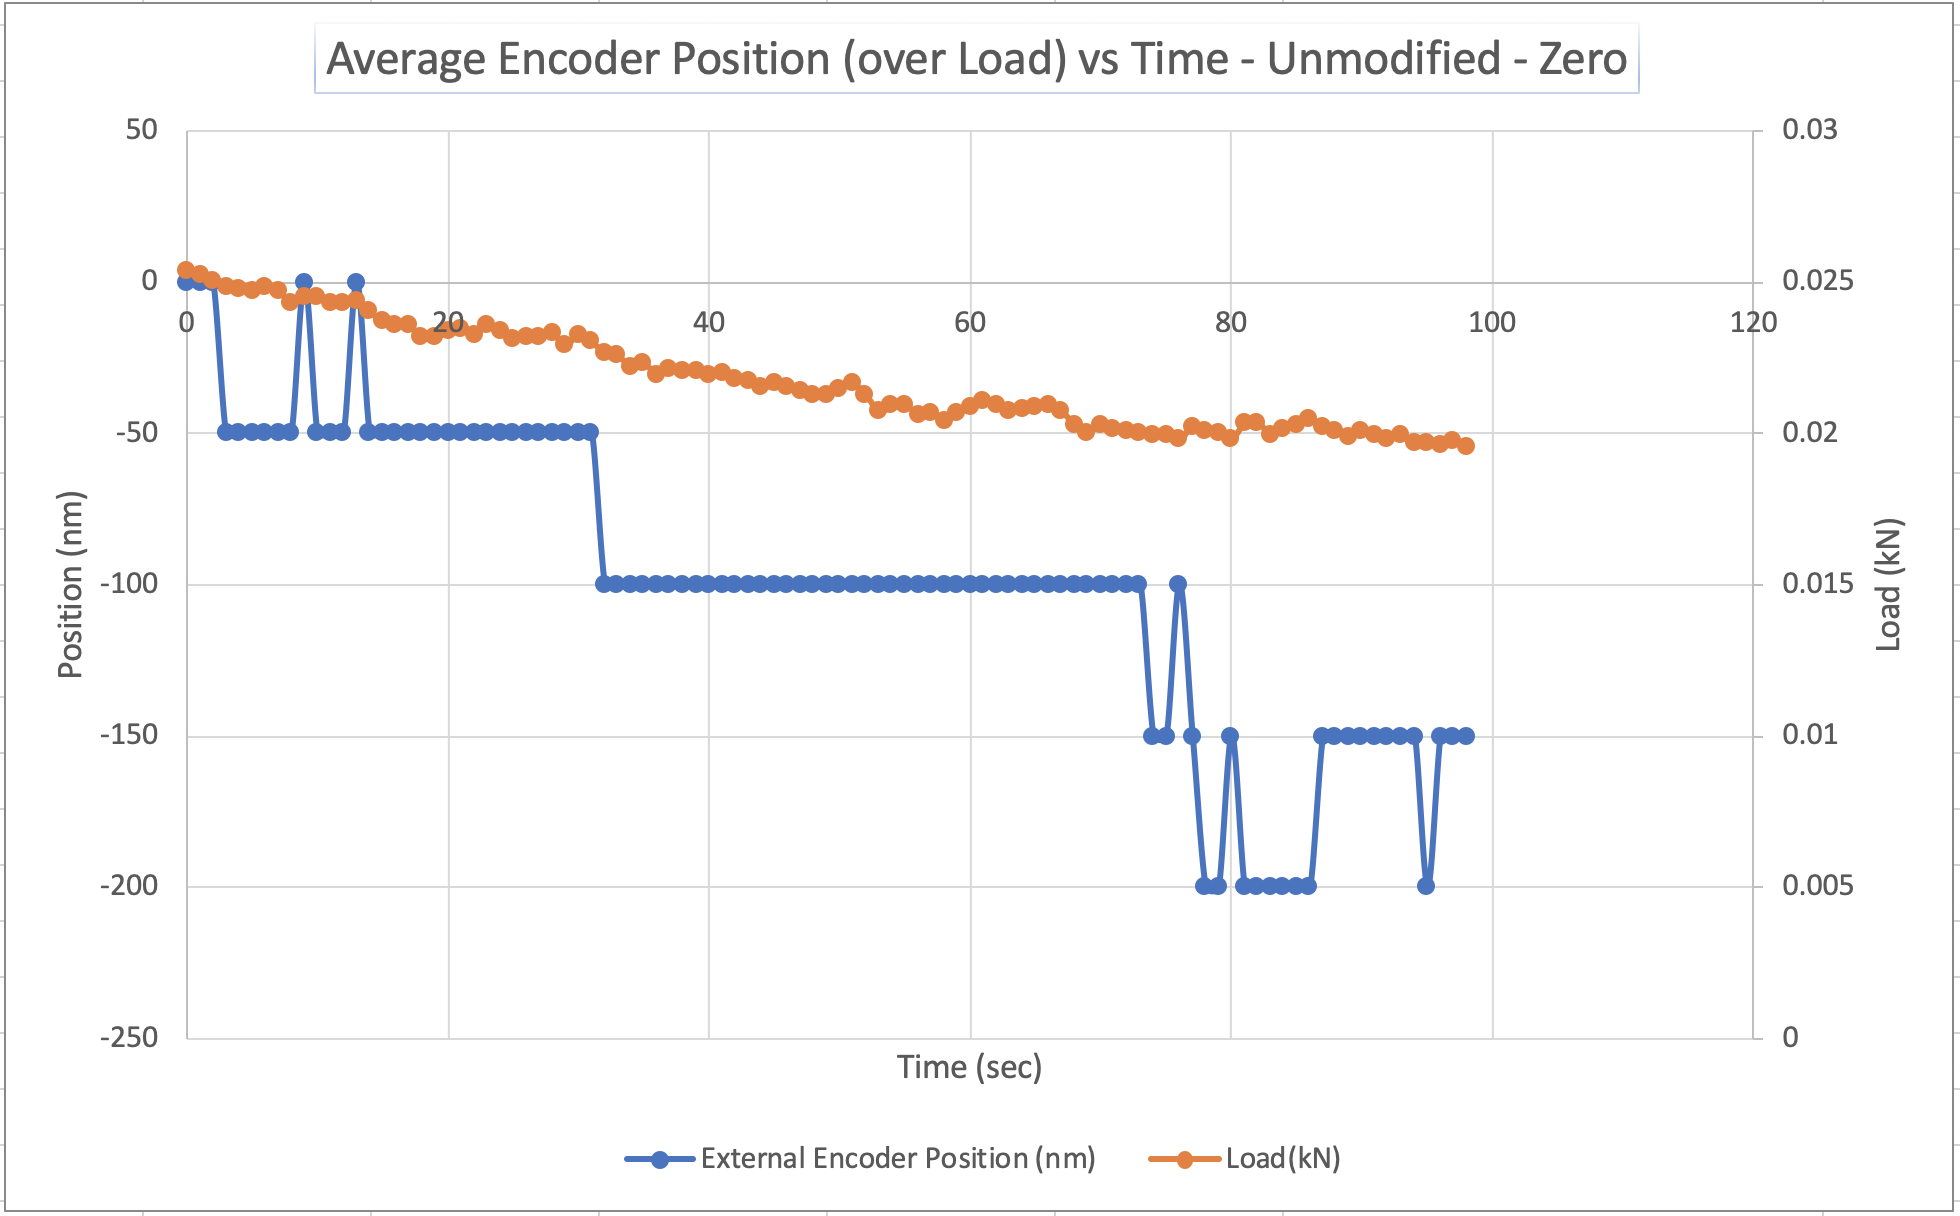
\includegraphics[width=5.98958in]{jira_imgs/4019.png}Note: Even with the
tension and compression valves set to zero, we could not achieve an
absolute zero load.

}
\begin{tabular}{p{2cm}p{14cm}}
\toprule
Step 20 & Step Execution Status: \textbf{ Pass } \\ \hline
\end{tabular}
 Description \\
{\footnotesize
Record the actual displacement as measured by the internal encoder using
copley software.

}
\hdashrule[0.5ex]{\textwidth}{1pt}{3mm}
  Expected Result \\
{\footnotesize
Actual displacement measured by the internal encoder recorded in the
Copley Software.

}
\hdashrule[0.5ex]{\textwidth}{1pt}{3mm}
  Actual Result \\
{\footnotesize
The Active Load Position reported by the Copley Control Software could
not be exported. However, we confirmed after every move that the
relative motion moved +/-100nm each command as reported by the Copley
Control Software.

}
\begin{tabular}{p{2cm}p{14cm}}
\toprule
Step 21 & Step Execution Status: \textbf{ Pass } \\ \hline
\end{tabular}
 Description \\
{\footnotesize
Compare the internal linear encoder measurement with the average of the
two external linear encoder measurements.

}
\hdashrule[0.5ex]{\textwidth}{1pt}{3mm}
  Expected Result \\
{\footnotesize
The magnitude should not vary by more than 50\% from the commanded value
based on an average of the two external linear encoder measurements.

}
\hdashrule[0.5ex]{\textwidth}{1pt}{3mm}
  Actual Result \\
{\footnotesize
The average displacement did not vary by more than 50nm during the
sequence of moves.\\[2\baselineskip]This can be seen in column K of the
Zero sheet in the \emph{Resolution Test Results - Unmodified
Actuator.xlsx~}excel document.

}
\begin{tabular}{p{2cm}p{14cm}}
\toprule
Step 22 & Step Execution Status: \textbf{ Pass } \\ \hline
\end{tabular}
 Description \\
{\footnotesize
Press Stop button in the VI file front panel to stop reading of the
components.

}
\hdashrule[0.5ex]{\textwidth}{1pt}{3mm}
  Expected Result \\
{\footnotesize
Graphs in the front panel of the VI file becomes static.

}
\hdashrule[0.5ex]{\textwidth}{1pt}{3mm}
  Actual Result \\
{\footnotesize
The VI's were stopped.

}
\begin{tabular}{p{2cm}p{14cm}}
\toprule
Step 23 & Step Execution Status: \textbf{ Pass } \\ \hline
\end{tabular}
 Description \\
{\footnotesize
Check if all the test results are recorded in excel spreadsheets.~

}
\hdashrule[0.5ex]{\textwidth}{1pt}{3mm}
  Expected Result \\
{\footnotesize
Test Results are recorded in the excel spreadsheets residing in the
LabView Folder directory.~

}
\hdashrule[0.5ex]{\textwidth}{1pt}{3mm}
  Actual Result \\
{\footnotesize
All test results have been recorded and collected into the
\emph{Resolution Test Results - Unmodified Actuator.xlsx} excel
document.

}
\begin{tabular}{p{2cm}p{14cm}}
\toprule
Step 24 & Step Execution Status: \textbf{ Not Executed } \\ \hline
\end{tabular}
 Description \\
{\footnotesize
Close all the Labview VI files.

}
\hdashrule[0.5ex]{\textwidth}{1pt}{3mm}
  Test Data \\
 {\footnotesize
\textbf{Note:~}Labview can be left open in order to continue to the next
test. However, it may be necessary to reset the application before
starting the next test.

}
\hdashrule[0.5ex]{\textwidth}{1pt}{3mm}
  Expected Result \\
{\footnotesize
All the VI files are closed and Labview 2021 application window closes.~

}
\hdashrule[0.5ex]{\textwidth}{1pt}{3mm}
  Actual Result \\
{\footnotesize
The LabView VI's were stopped, but not closed.

}

\paragraph{ LVV-T2436 - Hexapod - Actuator Accuracy Test }\mbox{}\\

Version \textbf{1}.
Status \textbf{Approved}.
Open  \href{https://jira.lsstcorp.org/secure/Tests.jspa#/testCase/LVV-T2436}{\textit{ LVV-T2436 } }
test case in Jira.

To perform the actuator accuracy tests in order to verify the Hexapod
Accuracy requirements in \citeds{LTS-206}.~

\textbf{ Preconditions}:\\


Execution status: {\bf Pass }

Final comment:\\During this test, it can be seen in the results that there were
variations in the applied load that may have impacted the results of
this test. As a result of the noise, there were outliers to the expected
accuracy, specifically for the larger moves in mm. For the smaller moves
in um, the accuracy was less than the expected error. However, this was
expected as MOOG's original test report cites the same variation when
applying load. Therefore, load compensation was applied to the results
in an effort to reduce the noise's impact on the results. Applying load
compensation improved the overall results, but there were still some
outliers that were greater than the expected 17um for the large moves:

\begin{itemize}
\tightlist
\item
  Large scale accuracy maximum error - Tension = 14.3um
\item
  Large scale accuracy maximum error - Compression = \textbf{33.9um}
\item
  Large scale accuracy maximum error - Zero = \textbf{21.4um}
\end{itemize}

For the smaller moves, the maximum error was less than the expected
20um:

\begin{itemize}
\tightlist
\item
  Small scale accuracy maximum error - Tension = 8.7um
\item
  Small scale accuracy maximum error - Compression = 14um
\item
  Small scale accuracy maximum error - Zero = 10.25um
\end{itemize}


Detailed steps results:

\begin{tabular}{p{2cm}p{14cm}}
\toprule
Step 1 & Step Execution Status: \textbf{ Pass } \\ \hline
\end{tabular}
 Description \\
{\footnotesize
Review the Specification of the Resolute Encoder Series RL 36B ES 001 C
10 F encoder to confirm the accuracy of the encoder.

}
\hdashrule[0.5ex]{\textwidth}{1pt}{3mm}
  Expected Result \\
{\footnotesize
Accuracy should be less than 12um.

}
\hdashrule[0.5ex]{\textwidth}{1pt}{3mm}
  Actual Result \\
{\footnotesize
As seen on page 3 of the
\emph{RESOLUTE\_biss\_l-9517-9448-03-b(en).pdf,} the accuracy of the
RSLA Encoder is no more than +/-4um.

}
\begin{tabular}{p{2cm}p{14cm}}
\toprule
Step 2 & Step Execution Status: \textbf{ Pass } \\ \hline
\end{tabular}
 Description \\
{\footnotesize
Open Labview 2021 in the computer used for Test Setup.

}
\hdashrule[0.5ex]{\textwidth}{1pt}{3mm}
  Test Data \\
 {\footnotesize
The next three steps are conditional because these steps are included as
part of the Test Setup procedure and may not be necessary if LabView is
still open.

}
\hdashrule[0.5ex]{\textwidth}{1pt}{3mm}
  Expected Result \\
{\footnotesize
Labview 2021 opens successfully.

}
\hdashrule[0.5ex]{\textwidth}{1pt}{3mm}
  Actual Result \\
{\footnotesize
LabView and the required VI's were already opened at the start of the
execution of this test cycle.

}
\begin{tabular}{p{2cm}p{14cm}}
\toprule
Step 3 & Step Execution Status: \textbf{ Pass } \\ \hline
\end{tabular}
 Description \\
{\footnotesize
Run the following VI's:

\begin{itemize}
\tightlist
\item
  Encoder A (D13B) and Load Cell.vi
\item
  Encoder B (D0BD).vi
\end{itemize}

}
\hdashrule[0.5ex]{\textwidth}{1pt}{3mm}
  Expected Result \\
{\footnotesize
Front panel of VI's open without any error.

}
\hdashrule[0.5ex]{\textwidth}{1pt}{3mm}
  Actual Result \\
{\footnotesize
LabView was ran without any issue.‚Äã‚Äã‚Äã‚Äã

}
\begin{tabular}{p{2cm}p{14cm}}
\toprule
Step 4 & Step Execution Status: \textbf{ Pass } \\ \hline
\end{tabular}
 Description \\
{\footnotesize
Click Run button on the on the block diagram toolbar of the Labview VI
front panel.

}
\hdashrule[0.5ex]{\textwidth}{1pt}{3mm}
  Expected Result \\
{\footnotesize
LabView VI and associated sub Vi runs successfully. The graphs should
start to be populated with data once the run button is pressed.

}
\hdashrule[0.5ex]{\textwidth}{1pt}{3mm}
  Actual Result \\
{\footnotesize
LabView was ran without any issue.

}
\begin{tabular}{p{2cm}p{14cm}}
\toprule
Step 5 & Step Execution Status: \textbf{ Pass } \\ \hline
\end{tabular}
 Description \\
{\footnotesize
Position the actuator at its center of stroke position using the control
box and copley software.\\[2\baselineskip]

}
\hdashrule[0.5ex]{\textwidth}{1pt}{3mm}
  Test Data \\
 {\footnotesize
\textbf{Note:~}The original zero position/center of stroke position was
determined to be a linear encoder reading of 40mm. For the purpose of
this test, the same center of stroke position will be used.

}
\hdashrule[0.5ex]{\textwidth}{1pt}{3mm}
  Expected Result \\
{\footnotesize
Actuator positioned at its center of stroke position ~confirmed by
encoder reading in the LabView.\\[2\baselineskip]

}
\hdashrule[0.5ex]{\textwidth}{1pt}{3mm}
  Actual Result \\
{\footnotesize
During the execution of the Hexapod - Actuator Test Set Up (See
\href{https://jira.lsstcorp.org/secure/Tests.jspa\#/testPlayer/testExecution/LVV-E2735}{LVV-E2735}),
the center stroke position was determined to be -40.202mm. Therefore,
the actuator was commanded to this position and then zeroed. This
allowed commands to be sent in absolute moves.

}
\begin{tabular}{p{2cm}p{14cm}}
\toprule
Step 6 & Step Execution Status: \textbf{ Pass } \\ \hline
\end{tabular}
 Description \\
{\footnotesize
Apply a force of +15kN.

}
\hdashrule[0.5ex]{\textwidth}{1pt}{3mm}
  Test Data \\
 {\footnotesize
\textbf{Note:~}In order to apply a tension force of +15 kN, set Channel
1 = 2.19V and Channel 0 = 0V.

}
\hdashrule[0.5ex]{\textwidth}{1pt}{3mm}
  Expected Result \\
{\footnotesize
Load cell reader shows the applied +15 kN \textbf{tension} force.\\
LabView displays the voltage being applied.

}
\hdashrule[0.5ex]{\textwidth}{1pt}{3mm}
  Actual Result \\
{\footnotesize
Set the tension valve to 2.19V which applied a +14.94kN force

}
\begin{tabular}{p{2cm}p{14cm}}
\toprule
Step 7 & Step Execution Status: \textbf{ Pass } \\ \hline
\end{tabular}
 Description \\
{\footnotesize
Record the load cell value in the LabView in the form of Load vs Time
graph.

}
\hdashrule[0.5ex]{\textwidth}{1pt}{3mm}
  Expected Result \\
{\footnotesize
LabView load graph (Load vs Time) shows +15 kN tension force applied.

}
\hdashrule[0.5ex]{\textwidth}{1pt}{3mm}
  Actual Result \\
{\footnotesize
The values for load and displacement were exported from LabView in order
to create the following plot:\\
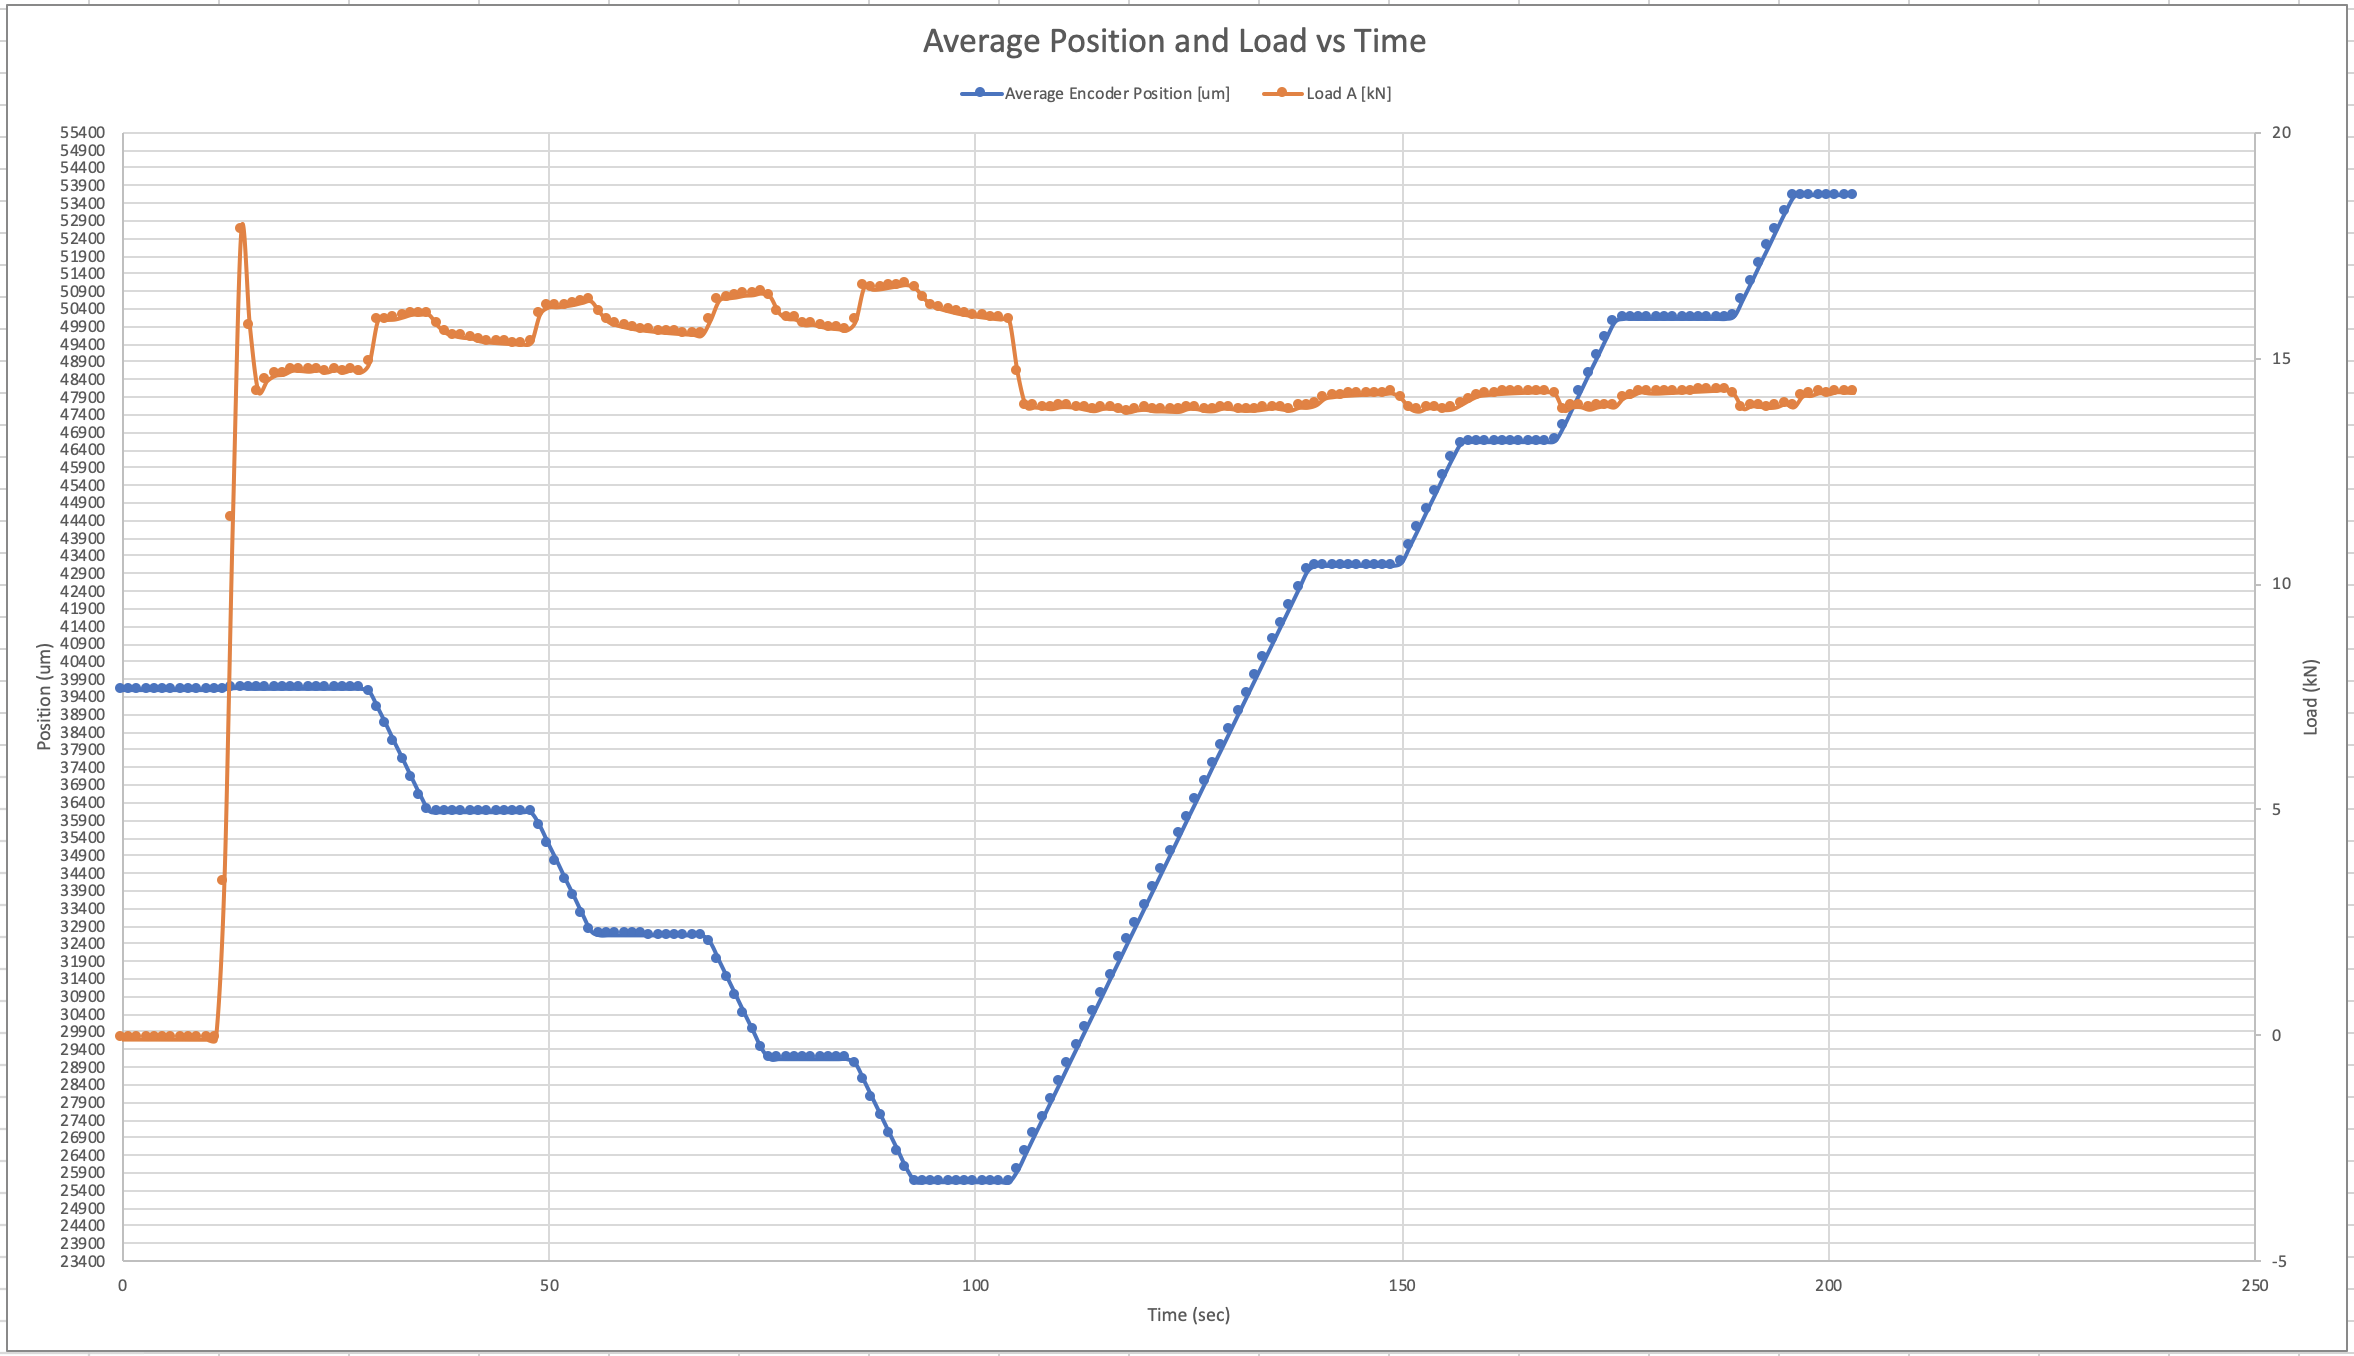
\includegraphics[width=5.98958in]{jira_imgs/4020.png}\\
This Average Position and Load vs. Time plot can be found on the Tension
- Large Scale sheet of the \emph{Accuracy Test Results - Unmodified
Actuator.xlsx} document

}
\begin{tabular}{p{2cm}p{14cm}}
\toprule
Step 8 & Step Execution Status: \textbf{ Pass } \\ \hline
\end{tabular}
 Description \\
{\footnotesize
Command the following moves to the actuator using the copley software
and the control box in absolute mode: +3.5mm, +7mm, +10.5mm, +14mm,
-3.5mm, -7mm, -10.5mm, -14mm.\\[2\baselineskip]

}
\hdashrule[0.5ex]{\textwidth}{1pt}{3mm}
  Expected Result \\
{\footnotesize
All moves should move in the commanded direction.

}
\hdashrule[0.5ex]{\textwidth}{1pt}{3mm}
  Actual Result \\
{\footnotesize
+3.5mm = 3500000 counts\\
Active Load Position = 3.49mm\\[2\baselineskip]+7mm = 7000000 counts\\
Active Load Position = 7.00mm\\[2\baselineskip]+10.5mm = 10500000
counts\\
Active Load Position = 10.50mm\\[2\baselineskip]+14mm = 14000000
counts\\
Active Load Position = 13.99mm\\[2\baselineskip]-3.5mm = 3500000
counts\\
Active Load Position = -3.49mm\\[2\baselineskip]-7mm = 7000000 counts\\
Active Load Position = -6.99mm\\[2\baselineskip]-10.5mm = 10500000
counts\\
Active Load Position = 10.49mm\\[2\baselineskip]-14mm = 14000000
counts\\
Active Load Position = -13.99mm

}
\begin{tabular}{p{2cm}p{14cm}}
\toprule
Step 9 & Step Execution Status: \textbf{ Pass } \\ \hline
\end{tabular}
 Description \\
{\footnotesize
Record the actual displacement as measured by the two external encoders
as LabView graph (Displacement vs Time).

}
\hdashrule[0.5ex]{\textwidth}{1pt}{3mm}
  Expected Result \\
{\footnotesize
Actual displacement measured by the average of the two external encoders
~recorded in the LabView graph.

}
\hdashrule[0.5ex]{\textwidth}{1pt}{3mm}
  Actual Result \\
{\footnotesize
The recorded data was exported from LabView into the Accuracy-Large
Scale sheet of the
\href{https://docushare.lsst.org/docushare/dsweb/Services/Document-55067}{\emph{Accuracy
Test Results -Modified vs Unmodified.xlsx}}excel document. The plotted
values can be seen below, where the blue and orange line represents the
average displacement of the external encoders and the grey line
represents the commanded position:\\
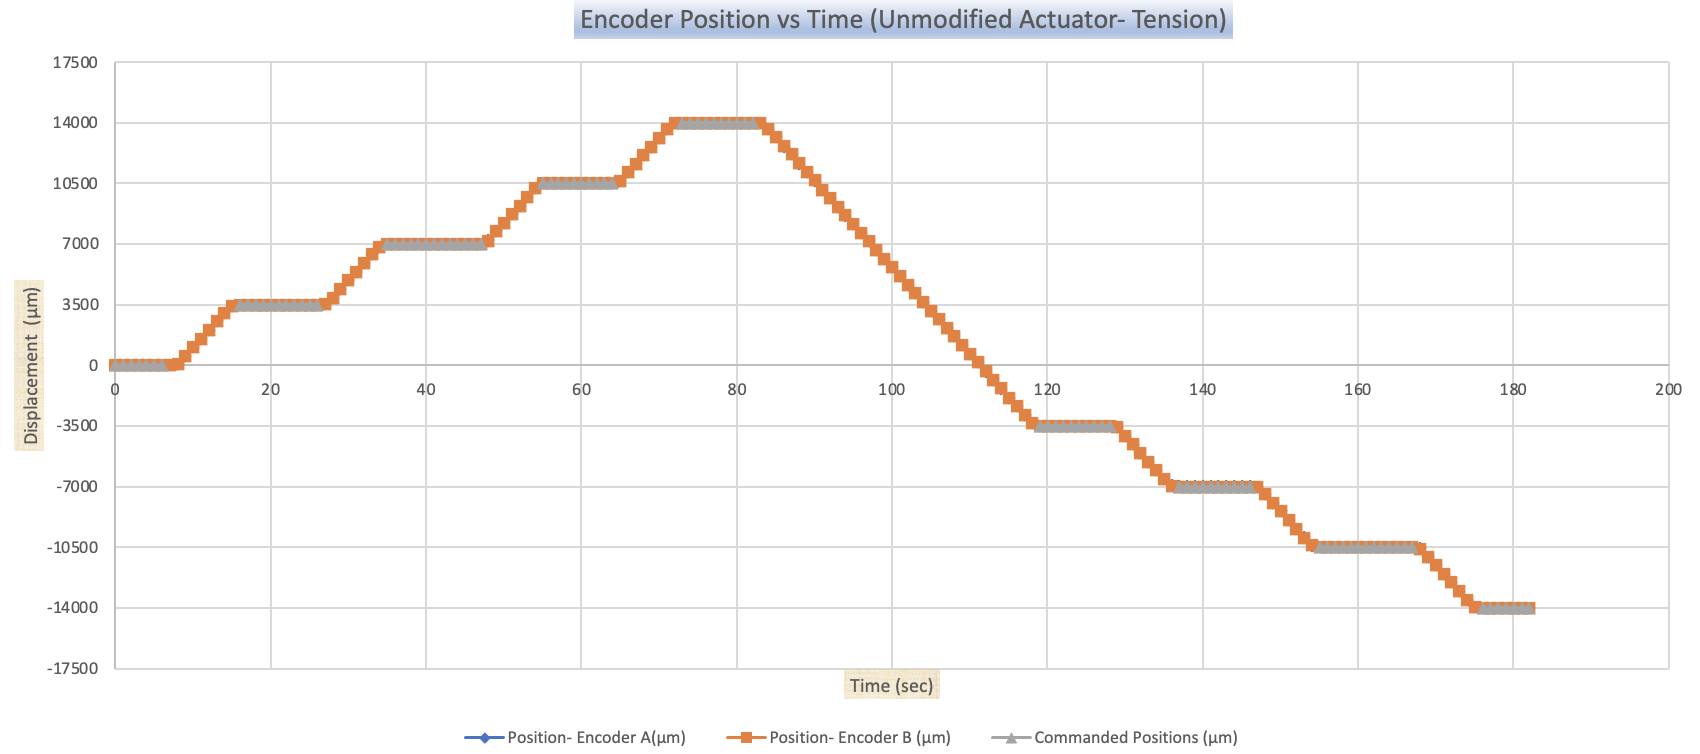
\includegraphics[width=5.98958in]{jira_imgs/4059.png}

}
\begin{tabular}{p{2cm}p{14cm}}
\toprule
Step 10 & Step Execution Status: \textbf{ Pass } \\ \hline
\end{tabular}
 Description \\
{\footnotesize
Record the actual displacement as measured by the internal encoder using
copley software.

}
\hdashrule[0.5ex]{\textwidth}{1pt}{3mm}
  Expected Result \\
{\footnotesize
Actual displacement measured by the internal encoder recorded in the
Copley Software.

}
\hdashrule[0.5ex]{\textwidth}{1pt}{3mm}
  Actual Result \\
{\footnotesize
The Active Load Position reported by the Copley Control Software could
not be exported. However, we confirmed the absolute position movements
as reported by the Copley Control Software.

}
\begin{tabular}{p{2cm}p{14cm}}
\toprule
Step 11 & Step Execution Status: \textbf{ Pass } \\ \hline
\end{tabular}
 Description \\
{\footnotesize
Ensure that the load cell signal did not vary significantly during the
test which would introduce compliance errors.

}
\hdashrule[0.5ex]{\textwidth}{1pt}{3mm}
  Expected Result \\
{\footnotesize
The tension load should remain close to +15kN throughout the
displacement movements and display in the Load vs Time graph in LabView.

}
\hdashrule[0.5ex]{\textwidth}{1pt}{3mm}
  Actual Result \\
{\footnotesize
There were some variations to the load while the actuator was moved.
Therefore, load compensation was applied similar to MOOG's procedure. As
a result, the average accuracy error can be seen below in orange:\\
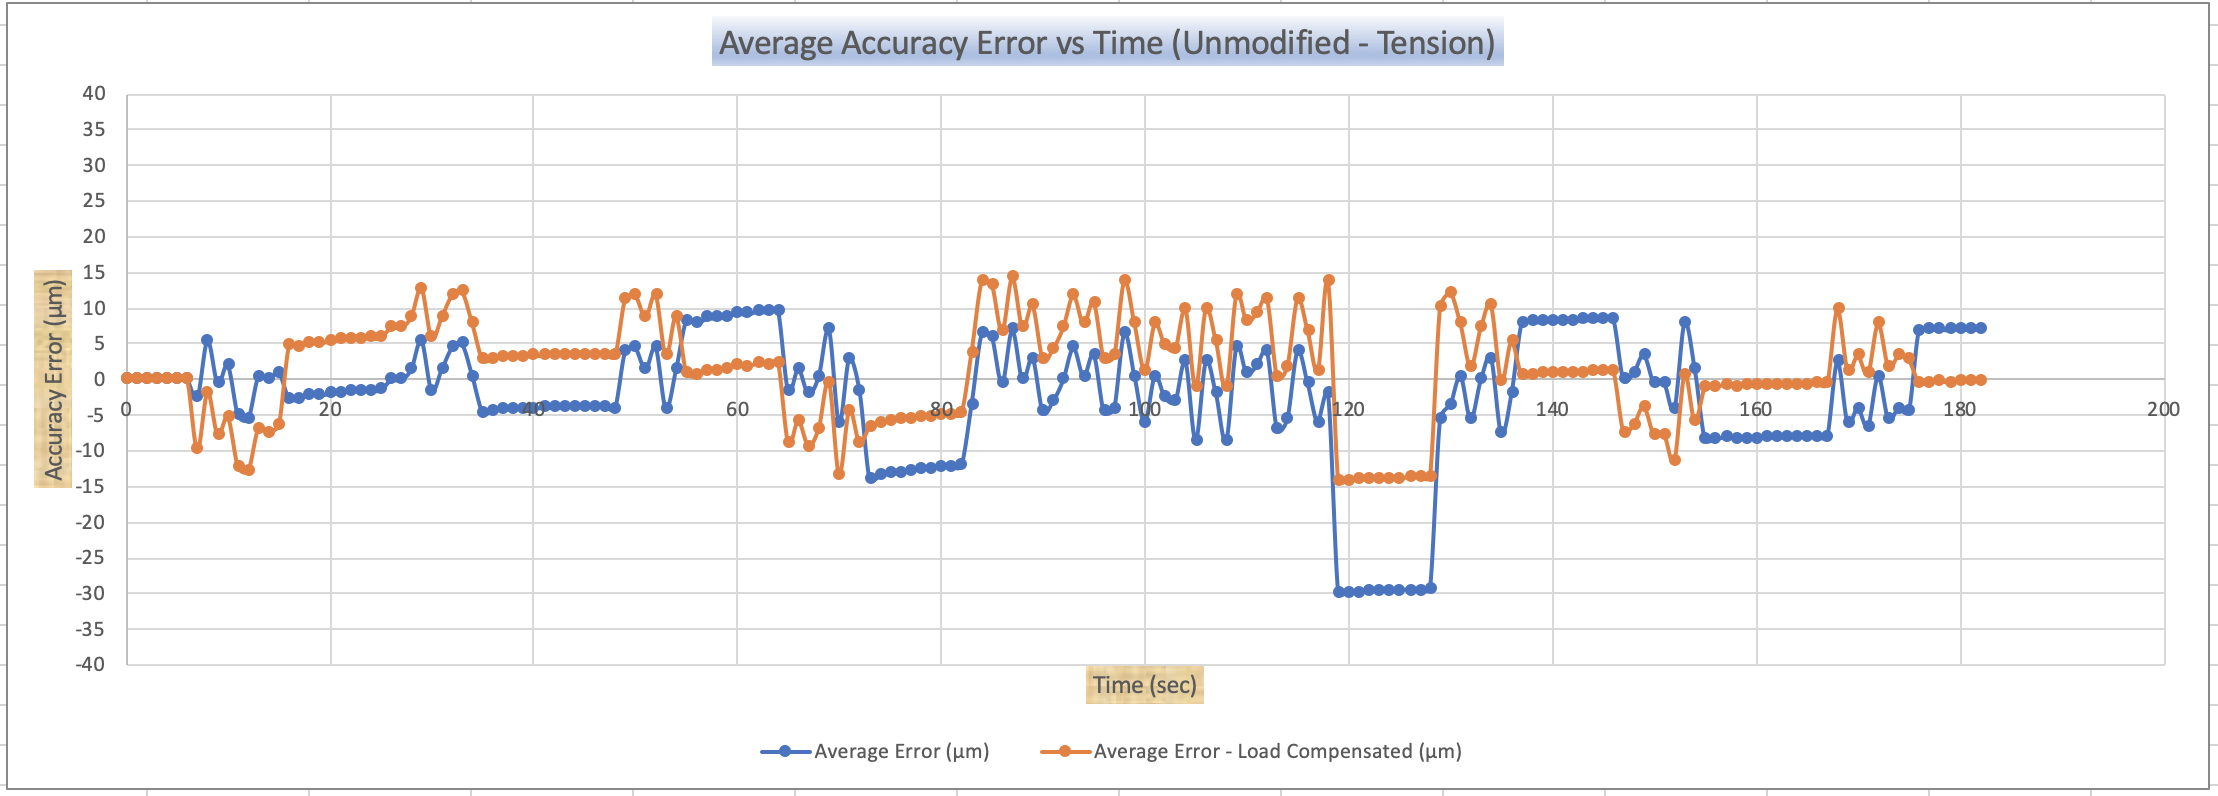
\includegraphics[width=5.98958in]{jira_imgs/4022.png}With the load
compensation, the average accuracy error was significantly reduced. This
plot can be found on the~Accuracy- Large Scale~sheet of
the\emph{~Accuracy Test Results -Modified vs Unmodifed.xlsx} document.

}
\begin{tabular}{p{2cm}p{14cm}}
\toprule
Step 12 & Step Execution Status: \textbf{ Pass } \\ \hline
\end{tabular}
 Description \\
{\footnotesize
Compare the internal linear encoder measurement with the average of the
two external linear encoder measurements in LabView.

}
\hdashrule[0.5ex]{\textwidth}{1pt}{3mm}
  Expected Result \\
{\footnotesize
\textbf{The large-scale accuracy error \textless{}= 17um.}

}
\hdashrule[0.5ex]{\textwidth}{1pt}{3mm}
  Actual Result \\
{\footnotesize
The internal encoder measurements were not measured during the
unmodified actuator tests. However, by analyzing the data from the
external linear encoder measurements, the large-scale accuracy error was
seen to be within \textless{}= 17um with load compensation. This can be
seen in the Average Accuracy Error vs. Time (Unmodified - Tension) plot
in the previous step.

}
\begin{tabular}{p{2cm}p{14cm}}
\toprule
Step 13 & Step Execution Status: \textbf{ Pass } \\ \hline
\end{tabular}
 Description \\
{\footnotesize
Restart at the zero position.

}
\hdashrule[0.5ex]{\textwidth}{1pt}{3mm}
  Test Data \\
 {\footnotesize
\textbf{Note:~}Command the actuator to the absolute zero position.

}
\hdashrule[0.5ex]{\textwidth}{1pt}{3mm}
  Expected Result \\
{\footnotesize
Actuator positioned at its center of stroke position ~confirmed by
encoder reading in the LabView.

}
\hdashrule[0.5ex]{\textwidth}{1pt}{3mm}
  Actual Result \\
{\footnotesize
The actuator was commanded back to the absolute zero position.\\
Active Load Position after commanding back to absolute zero position =
0.000666mm

}
\begin{tabular}{p{2cm}p{14cm}}
\toprule
Step 14 & Step Execution Status: \textbf{ Pass } \\ \hline
\end{tabular}
 Description \\
{\footnotesize
With a +15kN tension load applied to the actuator, command the following
moves the copley software and the control box in absolute mode: +100um,
+200um, +300um, +400um, -100um, -200um, -300um, -400um.

}
\hdashrule[0.5ex]{\textwidth}{1pt}{3mm}
  Expected Result \\
{\footnotesize
All moves should move in the commanded direction.

}
\hdashrule[0.5ex]{\textwidth}{1pt}{3mm}
  Actual Result \\
{\footnotesize
+100um\\
Active Load Position = 0.0999mm\\[2\baselineskip]+200um\\
Active Load Position = 0.1999mm\\[2\baselineskip]+300um\\
Active Load Position = 0.3000mm\\[2\baselineskip]+400um\\
Active Load Position = 0.3999mm\\[2\baselineskip]-100um\\
Active Load Position = -0.1000mm\\[2\baselineskip]-200um\\
Active Load Position = -0.1999mm\\[2\baselineskip]-300um\\
Active Load Position = -0.2999mm\\[2\baselineskip]-400um\\
Active Load Position = -0.3999mm

}
\begin{tabular}{p{2cm}p{14cm}}
\toprule
Step 15 & Step Execution Status: \textbf{ Pass } \\ \hline
\end{tabular}
 Description \\
{\footnotesize
Record the actual displacement as measured by the two external encoders
as LabView graph (Displacement vs Time).

}
\hdashrule[0.5ex]{\textwidth}{1pt}{3mm}
  Expected Result \\
{\footnotesize
Actual displacement measured by the average of the two external encoders
~recorded in the LabView graph.

}
\hdashrule[0.5ex]{\textwidth}{1pt}{3mm}
  Actual Result \\
{\footnotesize
The recorded data was exported from LabView into the Accuracy-Small
Scale sheet of the ~\emph{Accuracy Test Results -Modified vs
Unmodified.xlsx} excel document. The plotted values can be seen below
where the blue line represents the average displacement of the external
encoders and the orange line represents the commanded position:\\
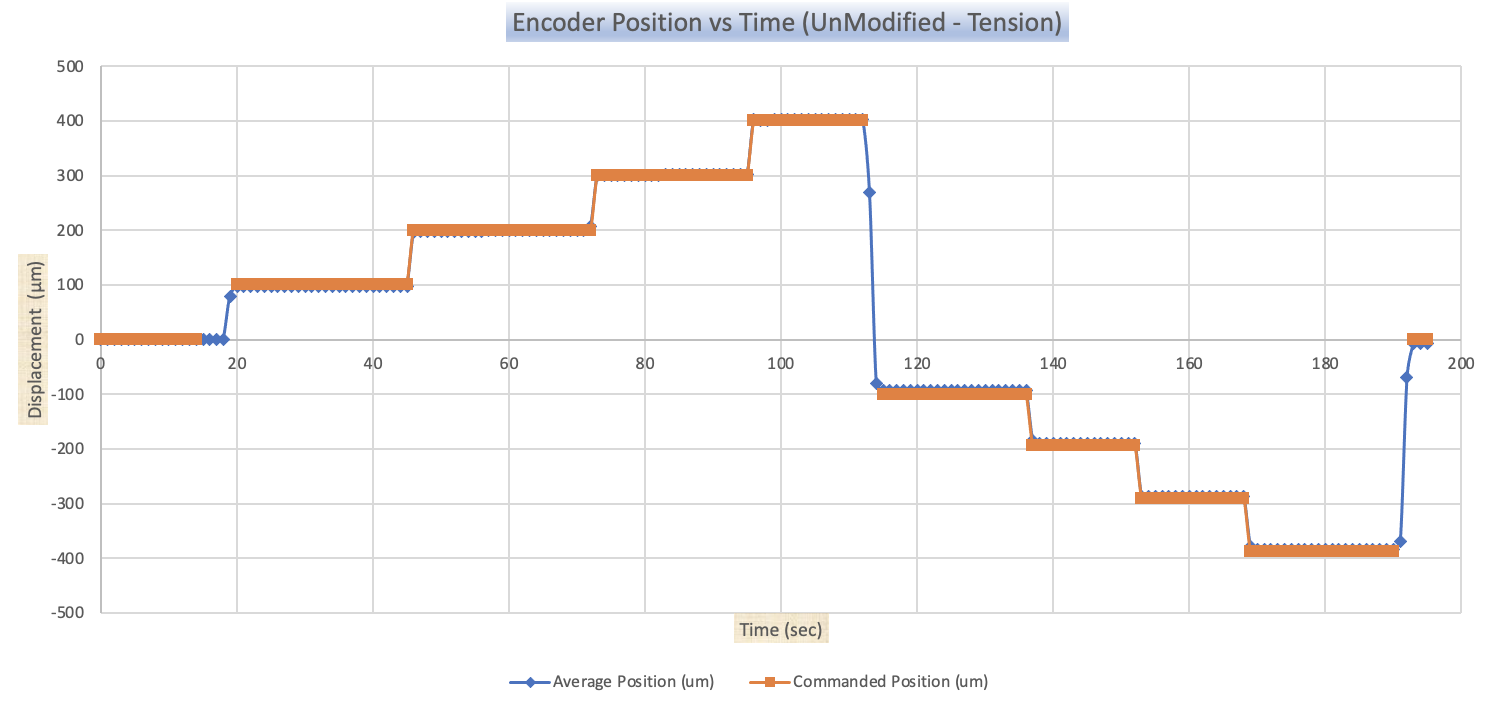
\includegraphics[width=5.98958in]{jira_imgs/4073.png}

}
\begin{tabular}{p{2cm}p{14cm}}
\toprule
Step 16 & Step Execution Status: \textbf{ Pass } \\ \hline
\end{tabular}
 Description \\
{\footnotesize
Record the actual displacement as measured by the internal encoder using
copley software.

}
\hdashrule[0.5ex]{\textwidth}{1pt}{3mm}
  Expected Result \\
{\footnotesize
Actual displacement measured by the internal encoder recorded in the
Copley Software.

}
\hdashrule[0.5ex]{\textwidth}{1pt}{3mm}
  Actual Result \\
{\footnotesize
The Active Load Position reported by the Copley Control Software could
not be exported. However, we monitored the absolute position movements
at the time of the test as reported by the Copley Control Software.

}
\begin{tabular}{p{2cm}p{14cm}}
\toprule
Step 17 & Step Execution Status: \textbf{ Pass } \\ \hline
\end{tabular}
 Description \\
{\footnotesize
Ensure that the load cell signal did not vary significantly during the
test which would introduce compliance errors.

}
\hdashrule[0.5ex]{\textwidth}{1pt}{3mm}
  Expected Result \\
{\footnotesize
The tension load should remain close to 15kN throughout the test and
display in the Load vs Time graph in LabView.

}
\hdashrule[0.5ex]{\textwidth}{1pt}{3mm}
  Actual Result \\
{\footnotesize
As seen in the plot attached to Step 15, the variation in load did not
have any significant impact to the actuator's ability to comply to the
commanded position. As a result, the average accuracy error can be seen
below in blue:\\
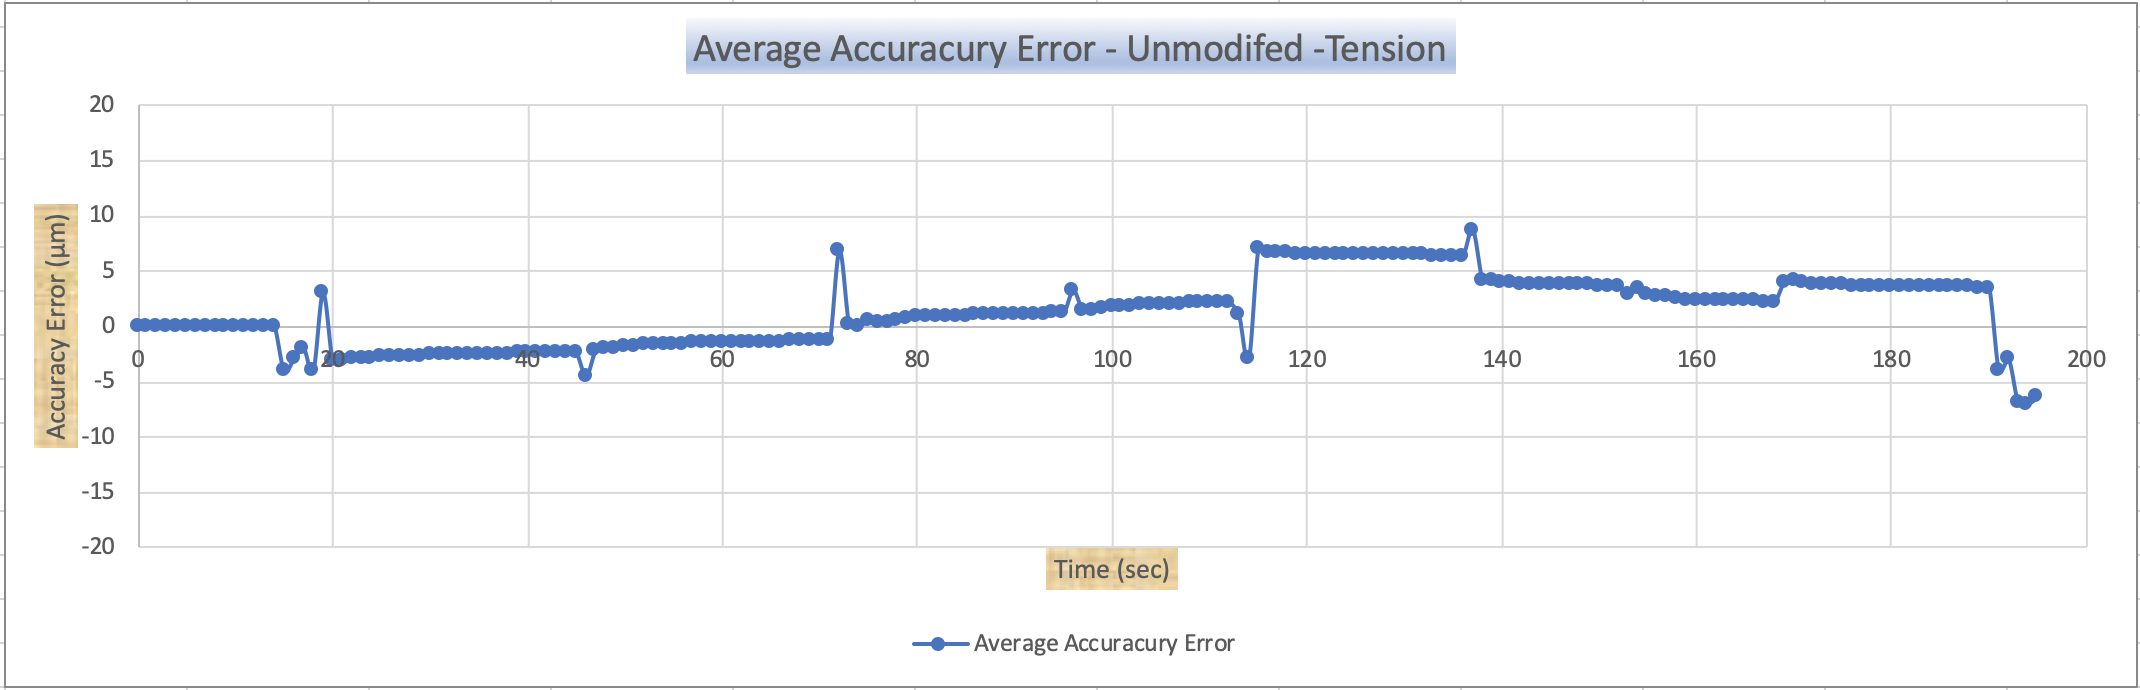
\includegraphics[width=5.98958in]{jira_imgs/4024.png}\\
This plot can be found on the~Accuracy- Small Scale~sheet of
the\emph{~Accuracy Test Results -Modified vs Unmodifed.xlsx} document.

}
\begin{tabular}{p{2cm}p{14cm}}
\toprule
Step 18 & Step Execution Status: \textbf{ Pass } \\ \hline
\end{tabular}
 Description \\
{\footnotesize
Compare the internal linear encoder measurement with the average of the
two external linear encoder measurements.

}
\hdashrule[0.5ex]{\textwidth}{1pt}{3mm}
  Expected Result \\
{\footnotesize
\textbf{The small-scale accuracy error \textless{}= 20um.}

}
\hdashrule[0.5ex]{\textwidth}{1pt}{3mm}
  Actual Result \\
{\footnotesize
The internal encoder measurements were not measured during the
unmodified actuator tests. However, by analyzing the data from the
external linear encoder measurements, the small-scale accuracy error was
seen to be within \textless{}= 20um with load compensation. This can be
seen in the Average Accuracy Error - Unmodified - Tension plot in the
previous step.

}
\begin{tabular}{p{2cm}p{14cm}}
\toprule
Step 19 & Step Execution Status: \textbf{ Pass } \\ \hline
\end{tabular}
 Description \\
{\footnotesize
Remove the 15 kN tension load.

}
\hdashrule[0.5ex]{\textwidth}{1pt}{3mm}
  Test Data \\
 {\footnotesize
\textbf{Note:~}Set Channel 0 = Channel 1 = 0V.

}
\hdashrule[0.5ex]{\textwidth}{1pt}{3mm}
  Expected Result \\
{\footnotesize
Load cell reader and Load graph in the LabView showing zero load.

}
\hdashrule[0.5ex]{\textwidth}{1pt}{3mm}
  Actual Result \\
{\footnotesize
The tension force was removed

}
\begin{tabular}{p{2cm}p{14cm}}
\toprule
Step 20 & Step Execution Status: \textbf{ Pass } \\ \hline
\end{tabular}
 Description \\
{\footnotesize
Restart at the zero position.

}
\hdashrule[0.5ex]{\textwidth}{1pt}{3mm}
  Test Data \\
 {\footnotesize
\textbf{Note:~}Command the actuator to the absolute zero position.

}
\hdashrule[0.5ex]{\textwidth}{1pt}{3mm}
  Expected Result \\
{\footnotesize
Actuator positioned at its center of stroke position ~confirmed by
encoder reading in the LabView.

}
\hdashrule[0.5ex]{\textwidth}{1pt}{3mm}
  Actual Result \\
{\footnotesize
The actuator was commanded back to the absolute zero position.

}
\begin{tabular}{p{2cm}p{14cm}}
\toprule
Step 21 & Step Execution Status: \textbf{ Pass } \\ \hline
\end{tabular}
 Description \\
{\footnotesize
Apply a -15kN force.

}
\hdashrule[0.5ex]{\textwidth}{1pt}{3mm}
  Test Data \\
 {\footnotesize
\textbf{Note:~}In order to apply a compression force of -15 kN, set
Channel 0 = 2.19V and Channel 1 = 0V.

}
\hdashrule[0.5ex]{\textwidth}{1pt}{3mm}
  Expected Result \\
{\footnotesize
Load cell reader shows the applied -15kN \textbf{compression} force.\\
LabView displays the voltage being applied.

}
\hdashrule[0.5ex]{\textwidth}{1pt}{3mm}
  Actual Result \\
{\footnotesize
Setting the Compression valve to 2.19V, a -14.9kN force was applied

}
\begin{tabular}{p{2cm}p{14cm}}
\toprule
Step 22 & Step Execution Status: \textbf{ Pass } \\ \hline
\end{tabular}
 Description \\
{\footnotesize
Command the following moves using the copley software and the control
box in absolute mode: +3.5mm, +7mm, +10.5mm, +14mm, -3.5mm, -7mm,
-10.5mm, -14mm.\\[2\baselineskip]

}
\hdashrule[0.5ex]{\textwidth}{1pt}{3mm}
  Expected Result \\
{\footnotesize
All moves should move in the commanded direction.

}
\hdashrule[0.5ex]{\textwidth}{1pt}{3mm}
  Actual Result \\
{\footnotesize
Active Load Position at zeroed position =
0.000134mm\\[2\baselineskip]+3.5mm = 3500000 counts\\
Active Load Position = 3.4976mm\\[2\baselineskip]+7mm = 7000000 counts\\
Active Load Position = 7.0001mm\\[2\baselineskip]+10.5mm = 10500000
counts\\
Active Load Position = 10.4999mm\\[2\baselineskip]+14mm = 14000000
counts\\
Active Load Position = 14.0002mm\\[2\baselineskip]-3.5mm = 3500000
counts\\
Active Load Position = -3.499mm\\[2\baselineskip]-7mm = 7000000 counts\\
Active Load Position = -6.992mm\\[2\baselineskip]-10.5mm = 10500000
counts\\
Active Load Position = -10.4992mm\\[2\baselineskip]-14mm = 14000000
counts\\
Active Load Position = -13.9999mm

}
\begin{tabular}{p{2cm}p{14cm}}
\toprule
Step 23 & Step Execution Status: \textbf{ Pass } \\ \hline
\end{tabular}
 Description \\
{\footnotesize
Record the actual displacement as measured by average of ~the two
external encoder as Labview graph (Displacement vs Time).

}
\hdashrule[0.5ex]{\textwidth}{1pt}{3mm}
  Expected Result \\
{\footnotesize
Actual displacement measured by the average of the two external encoders
~recorded in the LabView graph.

}
\hdashrule[0.5ex]{\textwidth}{1pt}{3mm}
  Actual Result \\
{\footnotesize
The recorded data was exported from LabView into the ``Accuracy-Large
Scale tab'' of the
~\href{https://docushare.lsst.org/docushare/dsweb/Get/Document-55067/Accuracy\%20Test\%20Results\%20-Modified\%20vs\%20Unmodified.xlsx}{\textbf{Accuracy
Test Results -Modified vs Unmodified.xlsx}} excel document. The plotted
values can be seen below where the blue and orange line represents the
average displacement of the external encoders and the grey line
represents the commanded
position:\\[2\baselineskip]\includegraphics[width=5.98958in]{jira_imgs/4052.png}

}
\begin{tabular}{p{2cm}p{14cm}}
\toprule
Step 24 & Step Execution Status: \textbf{ Pass } \\ \hline
\end{tabular}
 Description \\
{\footnotesize
Record the actual displacement as measured by the internal encoder using
copley software.

}
\hdashrule[0.5ex]{\textwidth}{1pt}{3mm}
  Expected Result \\
{\footnotesize
Actual displacement measured by the internal encoder recorded in the
Copley Software.

}
\hdashrule[0.5ex]{\textwidth}{1pt}{3mm}
  Actual Result \\
{\footnotesize
The Active Load Position reported by the Copley Control Software could
not be exported. However, we confirmed the absolute position movements
as reported by the Copley Control Software.

}
\begin{tabular}{p{2cm}p{14cm}}
\toprule
Step 25 & Step Execution Status: \textbf{ Pass } \\ \hline
\end{tabular}
 Description \\
{\footnotesize
Ensure that the load cell signal did not vary significantly during the
test which would introduce compliance errors.

}
\hdashrule[0.5ex]{\textwidth}{1pt}{3mm}
  Expected Result \\
{\footnotesize
The compression load should remain close to 15kN throughout the test and
display in the Load vs Time graph in LabView.

}
\hdashrule[0.5ex]{\textwidth}{1pt}{3mm}
  Actual Result \\
{\footnotesize
There were some variations to the load while the actuator was moved.
Therefore, load compensation was applied similar to MOOG's procedure. As
a result, the average accuracy error can be seen below in orange:\\
\includegraphics[width=5.98958in]{jira_imgs/4030.png}With the load
compensation, the average accuracy error was significantly reduced. This
Average Accuracy vs Time (Unmodified - Compression) plot can be found on
the~Accuracy- Large Scale~sheet of the\emph{~Accuracy Test Results
-Modified vs Unmodifed.xlsx} document.

}
\begin{tabular}{p{2cm}p{14cm}}
\toprule
Step 26 & Step Execution Status: \textbf{ Pass } \\ \hline
\end{tabular}
 Description \\
{\footnotesize
Compare the internal linear encoder measurement with the average of the
two external linear encoder measurements.

}
\hdashrule[0.5ex]{\textwidth}{1pt}{3mm}
  Expected Result \\
{\footnotesize
\textbf{The large-scale accuracy error \textless{}= 17um.}

}
\hdashrule[0.5ex]{\textwidth}{1pt}{3mm}
  Actual Result \\
{\footnotesize
The internal encoder measurements were not measured during the
unmodified actuator tests. However, by analyzing the data from the
external linear encoder measurements, the large-scale accuracy error was
seen to be mostly within \textless{}= 17um with load compensation. This
can be seen in the Average Accuracy Error vs. Time (Unmodified -
Compression) plot in the previous step. There were some outliers noted,
but this was expected as MOOG's original report showed noise on the load
cell and the external encoders. Although load compensation was applied,
there were still some errors that can be attributed to the noise. Since
this does not impact our ability to meet the hexapod level requirement,
this was marked as passed.

}
\begin{tabular}{p{2cm}p{14cm}}
\toprule
Step 27 & Step Execution Status: \textbf{ Pass } \\ \hline
\end{tabular}
 Description \\
{\footnotesize
Restart at the zero position.

}
\hdashrule[0.5ex]{\textwidth}{1pt}{3mm}
  Test Data \\
 {\footnotesize
\textbf{Note:~}The original zero position/center of stroke position was
determined to be a linear encoder reading of 40mm. For the purpose of
this test, the same center of stroke position will be used.

}
\hdashrule[0.5ex]{\textwidth}{1pt}{3mm}
  Expected Result \\
{\footnotesize
Actuator positioned at its center of stroke position ~confirmed by
encoder reading in the LabView.

}
\hdashrule[0.5ex]{\textwidth}{1pt}{3mm}
  Actual Result \\
{\footnotesize
The actuator was commanded back to the absolute zero position.\\
Active Load Position at the zeroed position = -0.000044mm

}
\begin{tabular}{p{2cm}p{14cm}}
\toprule
Step 28 & Step Execution Status: \textbf{ Pass } \\ \hline
\end{tabular}
 Description \\
{\footnotesize
With a 15 kN compression load applied to the actuator, command the
following moves using the copley software and the control box in
absolute mode: +100um, +200um, +300um, +400um, -100um, -200um, -300um,
-400um.

}
\hdashrule[0.5ex]{\textwidth}{1pt}{3mm}
  Expected Result \\
{\footnotesize
All moves should move in the commanded direction.

}
\hdashrule[0.5ex]{\textwidth}{1pt}{3mm}
  Actual Result \\
{\footnotesize
+100um = 100000 counts\\
Active Load Position = 0.1000mm\\[2\baselineskip]+200um = 200000
counts\\
Active Load Position = 0.1999mm\\[2\baselineskip]+300um = 300000
counts\\
Active Load Position = 0.3000mm\\[2\baselineskip]+400um = 400000
counts\\
Active Load Position = 0.4001mm\\[2\baselineskip]-100um = -100000
counts\\
Active Load Position = -0.0999mm\\[2\baselineskip]-200um = -200000
counts\\
Active Load Position = -0.1998mm\\[2\baselineskip]-300um =-300000
counts\\
Active Load Position = -0.2997mm\\[2\baselineskip]-400um = -400000
counts\\
Active Load Position = -0.3999mm

}
\begin{tabular}{p{2cm}p{14cm}}
\toprule
Step 29 & Step Execution Status: \textbf{ Pass } \\ \hline
\end{tabular}
 Description \\
{\footnotesize
Record the actual displacement as measured by average of ~the two
external encoder as Labview graph (Displacement vs. Time).

}
\hdashrule[0.5ex]{\textwidth}{1pt}{3mm}
  Expected Result \\
{\footnotesize
Actual displacement measured by the average of the two external encoders
~recorded in the LabView graph.

}
\hdashrule[0.5ex]{\textwidth}{1pt}{3mm}
  Actual Result \\
{\footnotesize
The recorded data was exported from LabView into the Accuracy-Small
Scale sheet of the \emph{Accuracy Test Results -Modified vs
Unmodified.xlsx} excel document. The plotted values can be seen below
where the blue line represents the average displacement of the external
encoders and the orange line represents the commanded position:\\
\includegraphics[width=5.98958in]{jira_imgs/4071.png}

}
\begin{tabular}{p{2cm}p{14cm}}
\toprule
Step 30 & Step Execution Status: \textbf{ Pass } \\ \hline
\end{tabular}
 Description \\
{\footnotesize
Record the actual displacement as measured by the internal encoder using
copley software.

}
\hdashrule[0.5ex]{\textwidth}{1pt}{3mm}
  Expected Result \\
{\footnotesize
Actual displacement measured by the internal encoder recorded in the
Copley Software.

}
\hdashrule[0.5ex]{\textwidth}{1pt}{3mm}
  Actual Result \\
{\footnotesize
The Active Load Position reported by the Copley Control Software could
not be exported. However, we monitored the absolute position movements
at the time of the test as reported by the Copley Control Software.

}
\begin{tabular}{p{2cm}p{14cm}}
\toprule
Step 31 & Step Execution Status: \textbf{ Pass } \\ \hline
\end{tabular}
 Description \\
{\footnotesize
Ensure that the load cell signal did not vary significantly during the
test which would introduce compliance errors.

}
\hdashrule[0.5ex]{\textwidth}{1pt}{3mm}
  Expected Result \\
{\footnotesize
The compression load should remain close to 15kN throughout the test and
displays in the Load vs Time graph in the LabView.

}
\hdashrule[0.5ex]{\textwidth}{1pt}{3mm}
  Actual Result \\
{\footnotesize
As seen in the plot attached to Step 29, the variation in load did not
have any significant impact to the actuator's ability to comply to the
commanded position. As a result, the average accuracy error can be seen
below in blue:\\
\includegraphics[width=5.98958in]{jira_imgs/4032.png}This Average
Accuracy Error (um) -Unmodified - Compression plot can be found on
the~Accuracy- Small Scale~sheet of the\emph{~Accuracy Test Results
-Modified vs Unmodifed.xlsx} document.

}
\begin{tabular}{p{2cm}p{14cm}}
\toprule
Step 32 & Step Execution Status: \textbf{ Pass } \\ \hline
\end{tabular}
 Description \\
{\footnotesize
Compare the internal linear encoder measurement with the average of the
two external linear encoder measurements.

}
\hdashrule[0.5ex]{\textwidth}{1pt}{3mm}
  Expected Result \\
{\footnotesize
\textbf{The small-scale accuracy error \textless{}= 20um.}

}
\hdashrule[0.5ex]{\textwidth}{1pt}{3mm}
  Actual Result \\
{\footnotesize
The internal encoder measurements were not measured during the
unmodified actuator tests. However, by analyzing the data from the
external linear encoder measurements, the small-scale accuracy error was
seen to be within \textless{}= 20um with load compensation. This can be
seen in the Average Accuracy Error (um) -Unmodified - Compression plot
in the previous step.

}
\begin{tabular}{p{2cm}p{14cm}}
\toprule
Step 33 & Step Execution Status: \textbf{ Pass } \\ \hline
\end{tabular}
 Description \\
{\footnotesize
Remove the 15 kN compression load.

}
\hdashrule[0.5ex]{\textwidth}{1pt}{3mm}
  Test Data \\
 {\footnotesize
\textbf{Note:~}Set Channel 0 = Channel 1 = 0V.

}
\hdashrule[0.5ex]{\textwidth}{1pt}{3mm}
  Expected Result \\
{\footnotesize
Load cell reader and Load graph in the LabView showing zero
load.\\[2\baselineskip]

}
\hdashrule[0.5ex]{\textwidth}{1pt}{3mm}
  Actual Result \\
{\footnotesize
Compression load was removed.~

}
\begin{tabular}{p{2cm}p{14cm}}
\toprule
Step 34 & Step Execution Status: \textbf{ Pass } \\ \hline
\end{tabular}
 Description \\
{\footnotesize
Restart at the zero position.

}
\hdashrule[0.5ex]{\textwidth}{1pt}{3mm}
  Test Data \\
 {\footnotesize
\textbf{Note:~}Command the actuator to the absolute zero position.

}
\hdashrule[0.5ex]{\textwidth}{1pt}{3mm}
  Expected Result \\
{\footnotesize
Actuator positioned at its center of stroke position ~confirmed by
encoder reading in the LabView.

}
\hdashrule[0.5ex]{\textwidth}{1pt}{3mm}
  Actual Result \\
{\footnotesize
The actuator was commanded back to the absolute zero position.~\\
Active Load Position at zeroed position = 0.000366mm

}
\begin{tabular}{p{2cm}p{14cm}}
\toprule
Step 35 & Step Execution Status: \textbf{ Pass } \\ \hline
\end{tabular}
 Description \\
{\footnotesize
With ``zero'' load applied to the actuator, command the following moves
using the copley software and the control box in absolute mode: +3.5mm,
+7mm, +10.5mm, +14mm, -3.5mm, -7mm, -10.5mm, -14mm.

}
\hdashrule[0.5ex]{\textwidth}{1pt}{3mm}
  Expected Result \\
{\footnotesize
All moves should move in the commanded direction.

}
\hdashrule[0.5ex]{\textwidth}{1pt}{3mm}
  Actual Result \\
{\footnotesize
+3.5mm = 3500000 counts\\
Active Load Position = 3.50mm\\[2\baselineskip]+7mm = 7000000 counts\\
Active Load Position = 7.00mm\\[2\baselineskip]+10.5mm = 10500000
counts\\
Active Load Position = 10.50mm\\[2\baselineskip]+14mm = 14000000
counts\\
Active Load Position = 14.00mm\\[2\baselineskip]-3.5mm = 3500000
counts\\
Active Load Position = -3.49mm\\[2\baselineskip]-7mm = 7000000 counts\\
Active Load Position = -6.99mm\\[2\baselineskip]-10.5mm = 10500000
counts\\
Active Load Position = -10.49mm\\[2\baselineskip]-14mm = 14000000
counts\\
Active Load Position = -13.99mm

}
\begin{tabular}{p{2cm}p{14cm}}
\toprule
Step 36 & Step Execution Status: \textbf{ Pass } \\ \hline
\end{tabular}
 Description \\
{\footnotesize
Record the actual displacement as measured by average of ~the two
external encoder as Labview graph (Displacement vs Time).

}
\hdashrule[0.5ex]{\textwidth}{1pt}{3mm}
  Expected Result \\
{\footnotesize
Actual displacement measured by the average of the two external encoders
~recorded in the LabView graph.

}
\hdashrule[0.5ex]{\textwidth}{1pt}{3mm}
  Actual Result \\
{\footnotesize
The recorded data was exported from LabView into the Accuracy-Large
Scale sheet of the \emph{Accuracy Test Results -Modified vs
Unmodified.xlsx} excel document. The plotted values can be seen below,
where the blue and orange line represents the average displacement of
the external encoders and the grey line represents the commanded
position:\\
\includegraphics[width=5.98958in]{jira_imgs/4048.png}

}
\begin{tabular}{p{2cm}p{14cm}}
\toprule
Step 37 & Step Execution Status: \textbf{ Pass } \\ \hline
\end{tabular}
 Description \\
{\footnotesize
Record the actual displacement as measured by the internal encoder using
copley software.

}
\hdashrule[0.5ex]{\textwidth}{1pt}{3mm}
  Expected Result \\
{\footnotesize
Actual displacement measured by the internal encoder recorded in the
Copley Software.

}
\hdashrule[0.5ex]{\textwidth}{1pt}{3mm}
  Actual Result \\
{\footnotesize
The Active Load Position reported by the Copley Control Software could
not be exported. However, we confirmed the absolute position movements
as reported by the Copley Control Software.

}
\begin{tabular}{p{2cm}p{14cm}}
\toprule
Step 38 & Step Execution Status: \textbf{ Pass } \\ \hline
\end{tabular}
 Description \\
{\footnotesize
Compare the internal linear encoder measurement with the average of the
two external linear encoder measurements.

}
\hdashrule[0.5ex]{\textwidth}{1pt}{3mm}
  Expected Result \\
{\footnotesize
\textbf{The large-scale accuracy error \textless{}= 17um.}

}
\hdashrule[0.5ex]{\textwidth}{1pt}{3mm}
  Actual Result \\
{\footnotesize
There were some variations to the load while the actuator was moved.
Therefore, load compensation was applied similar to MOOG's procedure. As
a result, the average accuracy error can be seen below in orange:\\
\includegraphics[width=5.98958in]{jira_imgs/4034.png}The internal
encoder measurements were not measured during the unmodified actuator
tests. However, by analyzing the data from the external linear encoder
measurements, the large-scale accuracy error was seen to be mostly
within \textless{}= 17um with load compensation. This can be seen in the
Average Accuracy Error vs. Time (Unmodified - Zero) plot in the previous
step. There were some outliers noted, but this was expected as MOOG's
original report showed noise on the load cell and the external encoders.
Although load compensation was applied, there were still some errors
that can be attributed to the noise. Since this does not impact our
ability to meet the hexapod level requirement, this was marked as
passed.

}
\begin{tabular}{p{2cm}p{14cm}}
\toprule
Step 39 & Step Execution Status: \textbf{ Pass } \\ \hline
\end{tabular}
 Description \\
{\footnotesize
Restart at the zero position.

}
\hdashrule[0.5ex]{\textwidth}{1pt}{3mm}
  Test Data \\
 {\footnotesize
\textbf{Note:~}Command the actuator to the absolute zero position.

}
\hdashrule[0.5ex]{\textwidth}{1pt}{3mm}
  Expected Result \\
{\footnotesize
Actuator positioned at its center of stroke position ~confirmed by
encoder reading in the LabView.

}
\hdashrule[0.5ex]{\textwidth}{1pt}{3mm}
  Actual Result \\
{\footnotesize
The actuator was commanded back to the absolute zero position.\\
Active Load Position at zeroed position = 0.000366mm

}
\begin{tabular}{p{2cm}p{14cm}}
\toprule
Step 40 & Step Execution Status: \textbf{ Pass } \\ \hline
\end{tabular}
 Description \\
{\footnotesize
With ``zero'' load applied to the actuator, command the following moves
using the copley software and the control box in absolute mode: +100um,
+200um, +300um, +400um, -100um, -200um, -300um, -400um.

}
\hdashrule[0.5ex]{\textwidth}{1pt}{3mm}
  Expected Result \\
{\footnotesize
All moves should move in the commanded direction.

}
\hdashrule[0.5ex]{\textwidth}{1pt}{3mm}
  Actual Result \\
{\footnotesize
+100um = 100000 counts\\
Active Load Position = 0.1002mm\\[2\baselineskip]+200um = 200000
counts\\
Active Load Position = 0.2002mm\\[2\baselineskip]+300um = 300000
counts\\
Active Load Position = 0.3000mm\\[2\baselineskip]+400um = 400000
counts\\
Active Load Position = 0.3999mm\\[2\baselineskip]-100um = -100000
counts\\
Active Load Position = -0.0999mm\\[2\baselineskip]-200um = -200000
counts\\
Active Load Position = -0.1999mm\\[2\baselineskip]-300um =-300000
counts\\
Active Load Position = -0.2999mm\\[2\baselineskip]-400um = -400000
counts\\
Active Load Position = -0.3999mm

}
\begin{tabular}{p{2cm}p{14cm}}
\toprule
Step 41 & Step Execution Status: \textbf{ Pass } \\ \hline
\end{tabular}
 Description \\
{\footnotesize
Record the actual displacement as measured by average of ~the two
external encoder as Labview graph (Displacement vs Time).

}
\hdashrule[0.5ex]{\textwidth}{1pt}{3mm}
  Expected Result \\
{\footnotesize
Actual displacement measured by the average of the two external encoders
~recorded in the LabView graph.

}
\hdashrule[0.5ex]{\textwidth}{1pt}{3mm}
  Actual Result \\
{\footnotesize
The recorded data was exported from LabView into the Accuracy-Small
Scale sheet of the
~\href{https://docushare.lsst.org/docushare/dsweb/Get/Document-55067/Accuracy\%20Test\%20Results\%20-Modified\%20vs\%20Unmodified.xlsx}{\textbf{Accuracy
Test Results -Modified vs Unmodified.xlsx}} excel document. The plotted
values can be seen below where the blue line represents the average
displacement of the external encoders and the orange line represents the
commanded position:\\
\includegraphics[width=5.98958in]{jira_imgs/4046.png}\\

}
\begin{tabular}{p{2cm}p{14cm}}
\toprule
Step 42 & Step Execution Status: \textbf{ Pass } \\ \hline
\end{tabular}
 Description \\
{\footnotesize
Record the actual displacement as measured by the internal encoder using
copley software.

}
\hdashrule[0.5ex]{\textwidth}{1pt}{3mm}
  Expected Result \\
{\footnotesize
Actual displacement measured by the internal encoder recorded in the
Copley Software.

}
\hdashrule[0.5ex]{\textwidth}{1pt}{3mm}
  Actual Result \\
{\footnotesize
The Active Load Position reported by the Copley Control Software could
not be exported. However, we monitored the absolute position movements
at the time of the test as reported by the Copley Control Software.

}
\begin{tabular}{p{2cm}p{14cm}}
\toprule
Step 43 & Step Execution Status: \textbf{ Pass } \\ \hline
\end{tabular}
 Description \\
{\footnotesize
Compare the internal linear encoder measurement with the average of the
two external linear encoder measurements.

}
\hdashrule[0.5ex]{\textwidth}{1pt}{3mm}
  Expected Result \\
{\footnotesize
\textbf{The small-scale accuracy error \textless{}= 20um.}

}
\hdashrule[0.5ex]{\textwidth}{1pt}{3mm}
  Actual Result \\
{\footnotesize
As seen in the plot attached to Step 41, there was some variation of
load seen at the time of the test. Therefore, load compensation was
applied similar to MOOG's procedure. As a result, the average accuracy
error can be seen below in blue:\\
\includegraphics[width=5.98958in]{jira_imgs/4041.png}As seen by the
plot, the average accuracy error was within 20um. This Average Accuracy
Error vs Time (UnModified - Zero) plot can be found on the~Accuracy-
Small Scale~sheet of the\emph{~Accuracy Test Results -Modified vs
Unmodifed.xlsx} document.

}
\begin{tabular}{p{2cm}p{14cm}}
\toprule
Step 44 & Step Execution Status: \textbf{ Pass } \\ \hline
\end{tabular}
 Description \\
{\footnotesize
Press Stop button in the VI file front panel to stop reading of the
components.

}
\hdashrule[0.5ex]{\textwidth}{1pt}{3mm}
  Expected Result \\
{\footnotesize
Graphs in the front panel of the VI file becomes static.

}
\hdashrule[0.5ex]{\textwidth}{1pt}{3mm}
  Actual Result \\
{\footnotesize
The LabView VI's were stopped.

}
\begin{tabular}{p{2cm}p{14cm}}
\toprule
Step 45 & Step Execution Status: \textbf{ Pass } \\ \hline
\end{tabular}
 Description \\
{\footnotesize
Check if all the test results are recorded in excel spreadsheets.

}
\hdashrule[0.5ex]{\textwidth}{1pt}{3mm}
  Expected Result \\
{\footnotesize
Test Results are recorded in the excel spreadsheets residing in the
LabView Folder directory.

}
\hdashrule[0.5ex]{\textwidth}{1pt}{3mm}
  Actual Result \\
{\footnotesize
All test results have been recorded and attached to the previous
steps.‚Äã‚Äã‚Äã‚Äã

}
\begin{tabular}{p{2cm}p{14cm}}
\toprule
Step 46 & Step Execution Status: \textbf{ Not Executed } \\ \hline
\end{tabular}
 Description \\
{\footnotesize
Close all the Labview VI files.

}
\hdashrule[0.5ex]{\textwidth}{1pt}{3mm}
  Test Data \\
 {\footnotesize
\textbf{Note:~}Labview can be left open in order to continue to the next
test. However, it may be necessary to reset the application before
starting the next test.

}
\hdashrule[0.5ex]{\textwidth}{1pt}{3mm}
  Expected Result \\
{\footnotesize
All the VI files are closed and Labview 2021 application window closes.

}
\hdashrule[0.5ex]{\textwidth}{1pt}{3mm}
  Actual Result \\
{\footnotesize
The LabView VI's were stopped, but not closed.

}

\paragraph{ LVV-T2435 - Hexapod - Actuator Repeatability Test }\mbox{}\\

Version \textbf{1}.
Status \textbf{Approved}.
Open  \href{https://jira.lsstcorp.org/secure/Tests.jspa#/testCase/LVV-T2435}{\textit{ LVV-T2435 } }
test case in Jira.

The objective of this test case will be to re-verify the hexapod
actuator repeatability requirements as stated in \citeds{LTS-206}. This will be
done by repeating a series of moves in order to verify that the
deviation between the sets of moves is not greater than 5um.~

\textbf{ Preconditions}:\\


Execution status: {\bf Pass }

Final comment:\\There were three iterations of this test, once with a +15kN load
applied, once with a -15kN load applied and once with no load applied.
For each test, the actuator was commanded through a series of four 500um
moves repeated five times. In order to determine the repeatability of
the actuator, the displacement was measured once the actuator had
completed its 500um move. As seen in the
\href{https://docushare.lsst.org/docushare/dsweb/Services/Document-55071}{\emph{Repeatability
Test Results -Modified vs Unmodified Actuator.xlsx}}\emph{~}file, the
repeatability error (calculated using rms method) was never seen to be
greater than 1um so this test was passed.


Detailed steps results:

\begin{tabular}{p{2cm}p{14cm}}
\toprule
Step 0.4 & Step Execution Status: \textbf{ Pass } \\ \hline
\end{tabular}
 Description \\
{\footnotesize
Start at a random actuator stroke position sufficiently away from the
software stroke limits.

}
\hdashrule[0.5ex]{\textwidth}{1pt}{3mm}
  Test Data \\
 {\footnotesize
\textbf{Note:~}The actuator stroke from hard stop to hard stop is
+/-19.36mm. The minimum amount required to meet hexapod range
requirements is +/-16.02mm.

}
\hdashrule[0.5ex]{\textwidth}{1pt}{3mm}
  Expected Result \\
{\footnotesize
Appropriate actuator stroke-position selected for the test.~

}
\hdashrule[0.5ex]{\textwidth}{1pt}{3mm}
  Actual Result \\
{\footnotesize
The starting position was the position we left off on from the previous
test.\\
Active Load Position = -40.203mm

}
\begin{tabular}{p{2cm}p{14cm}}
\toprule
Step 0.4 & Step Execution Status: \textbf{ Not Executed } \\ \hline
\end{tabular}
 Description \\
{\footnotesize
Start at a random actuator stroke position sufficiently away from the
software stroke limits.

}
\hdashrule[0.5ex]{\textwidth}{1pt}{3mm}
  Test Data \\
 {\footnotesize
\textbf{Note:~}The actuator stroke from hard stop to hard stop is
+/-19.36mm. The minimum amount required to meet hexapod range
requirements is +/-16.02mm.

}
\hdashrule[0.5ex]{\textwidth}{1pt}{3mm}
  Expected Result \\
{\footnotesize
Appropriate actuator stroke-position selected for the test.~

}
\hdashrule[0.5ex]{\textwidth}{1pt}{3mm}
  Actual Result \\
{\footnotesize
The actuator was positioned at the center most position (Copley measured
at -40.202mm) to start the test.

}
\begin{tabular}{p{2cm}p{14cm}}
\toprule
Step 0.4 & Step Execution Status: \textbf{ Not Executed } \\ \hline
\end{tabular}
 Description \\
{\footnotesize
Start at a random actuator stroke position sufficiently away from the
software stroke limits.

}
\hdashrule[0.5ex]{\textwidth}{1pt}{3mm}
  Test Data \\
 {\footnotesize
\textbf{Note:~}The actuator stroke from hard stop to hard stop is
+/-19.36mm. The minimum amount required to meet hexapod range
requirements is +/-16.02mm.

}
\hdashrule[0.5ex]{\textwidth}{1pt}{3mm}
  Expected Result \\
{\footnotesize
Appropriate actuator stroke-position selected for the test.~

}
\hdashrule[0.5ex]{\textwidth}{1pt}{3mm}
  Actual Result \\
{\footnotesize
The actuator was positioned at the center most position (Copley measured
at -40.202mm) to start the test.

}
\begin{tabular}{p{2cm}p{14cm}}
\toprule
Step 0.5 & Step Execution Status: \textbf{ Pass } \\ \hline
\end{tabular}
 Description \\
{\footnotesize
Apply a {15kN tension}⁠ load by using the LabView function to apply the
appropriate voltage values to the compression and tension air valves.

}
\hdashrule[0.5ex]{\textwidth}{1pt}{3mm}
  Test Data \\
 {\footnotesize
{\textbf{Note:}}

\begin{itemize}
\tightlist
\item
  {Tension test: Set Channel 1 = 2.19V and Channel 0 = 0V}
\item
  Zero Load test: Set Channel 1 = Channel 0 = 0V \textbf{~}
\item
  Compression test - Set Channel 1 = 0V and Channel 0 = 2.19V
\end{itemize}

}
\hdashrule[0.5ex]{\textwidth}{1pt}{3mm}
  Expected Result \\
{\footnotesize
The actuator has {15kN tension}⁠ load applied.

}
\hdashrule[0.5ex]{\textwidth}{1pt}{3mm}
  Actual Result \\
{\footnotesize
The Tension valve was set for 2.19V which applied a +14.89kN force.

}
\begin{tabular}{p{2cm}p{14cm}}
\toprule
Step 0.5 & Step Execution Status: \textbf{ Pass } \\ \hline
\end{tabular}
 Description \\
{\footnotesize
Apply a {zero}⁠ load by using the LabView function to apply the
appropriate voltage values to the compression and tension air valves.

}
\hdashrule[0.5ex]{\textwidth}{1pt}{3mm}
  Test Data \\
 {\footnotesize
{\textbf{Note:}}

\begin{itemize}
\tightlist
\item
  {Tension test: Set Channel 1 = 2.19V and Channel 0 = 0V}
\item
  Zero Load test: Set Channel 1 = Channel 0 = 0V \textbf{~}
\item
  Compression test - Set Channel 1 = 0V and Channel 0 = 2.19V
\end{itemize}

}
\hdashrule[0.5ex]{\textwidth}{1pt}{3mm}
  Expected Result \\
{\footnotesize
The actuator has {zero}⁠ load applied.

}
\hdashrule[0.5ex]{\textwidth}{1pt}{3mm}
  Actual Result \\
{\footnotesize
No load applied. At the zeroed position, Active Load Position reading
0.000126mm

}
\begin{tabular}{p{2cm}p{14cm}}
\toprule
Step 0.5 & Step Execution Status: \textbf{ Pass } \\ \hline
\end{tabular}
 Description \\
{\footnotesize
Apply a {15kN compression}⁠ load by using the LabView function to apply
the appropriate voltage values to the compression and tension air
valves.

}
\hdashrule[0.5ex]{\textwidth}{1pt}{3mm}
  Test Data \\
 {\footnotesize
{\textbf{Note:}}

\begin{itemize}
\tightlist
\item
  {Tension test: Set Channel 1 = 2.19V and Channel 0 = 0V}
\item
  Zero Load test: Set Channel 1 = Channel 0 = 0V \textbf{~}
\item
  Compression test - Set Channel 1 = 0V and Channel 0 = 2.19V
\end{itemize}

}
\hdashrule[0.5ex]{\textwidth}{1pt}{3mm}
  Expected Result \\
{\footnotesize
The actuator has {15kN compression}⁠ load applied.

}
\hdashrule[0.5ex]{\textwidth}{1pt}{3mm}
  Actual Result \\
{\footnotesize
The Compression valve was set for 2.19V which applied a -14.93kN force.

}
\begin{tabular}{p{2cm}p{14cm}}
\toprule
Step 0.6 & Step Execution Status: \textbf{ Pass } \\ \hline
\end{tabular}
 Description \\
{\footnotesize
Command the actuator to move to the absolute positions of +500um, 0um,
-500um, and then 0um.

}
\hdashrule[0.5ex]{\textwidth}{1pt}{3mm}
  Expected Result \\
{\footnotesize
The actuator moves to within 5um of the commanded absolute positions.

}
\hdashrule[0.5ex]{\textwidth}{1pt}{3mm}
  Actual Result \\
{\footnotesize
The sequence of moves were executed while Labview recorded the
displacement of the encoders.\\
\textbf{Note:} Commanding +500000 counts to the actuator resulted in a
smaller Encoder A displacement reading (\textasciitilde{}39.9mm to
\textasciitilde{}39.4mm), whereas commanding -500000 counts resulted in
a larger displacement (\textasciitilde{}39.9mm to
\textasciitilde{}40.3mm)\\
Same for Encoder B:\\
+500000 resulted in a displacement from (\textasciitilde{}39.4mm to
\textasciitilde{}38.9mm)\\
-500000 resulted in a displacement from (\textasciitilde{}39.8mm to
\textasciitilde{}40.3mm)

}
\begin{tabular}{p{2cm}p{14cm}}
\toprule
Step 0.6 & Step Execution Status: \textbf{ Pass } \\ \hline
\end{tabular}
 Description \\
{\footnotesize
Command the actuator to move to the absolute positions of +500um, 0um,
-500um, and then 0um.

}
\hdashrule[0.5ex]{\textwidth}{1pt}{3mm}
  Expected Result \\
{\footnotesize
The actuator moves to within 5um of the commanded absolute positions.

}
\hdashrule[0.5ex]{\textwidth}{1pt}{3mm}
  Actual Result \\
{\footnotesize
The sequence of moves was executed while Labview recorded the
displacement of the encoders.

}
\begin{tabular}{p{2cm}p{14cm}}
\toprule
Step 0.6 & Step Execution Status: \textbf{ Pass } \\ \hline
\end{tabular}
 Description \\
{\footnotesize
Command the actuator to move to the absolute positions of +500um, 0um,
-500um, and then 0um.

}
\hdashrule[0.5ex]{\textwidth}{1pt}{3mm}
  Expected Result \\
{\footnotesize
The actuator moves to within 5um of the commanded absolute positions.

}
\hdashrule[0.5ex]{\textwidth}{1pt}{3mm}
  Actual Result \\
{\footnotesize
The sequence of moves were executed while Labview recorded the
displacement of the encoders.

}
\begin{tabular}{p{2cm}p{14cm}}
\toprule
Step 0.7 & Step Execution Status: \textbf{ Pass } \\ \hline
\end{tabular}
 Description \\
{\footnotesize
Command the actuator to move to the absolute positions of +500um, 0um,
-500um, and then 0um.

}
\hdashrule[0.5ex]{\textwidth}{1pt}{3mm}
  Expected Result \\
{\footnotesize
The actuator moves to within 5um of the commanded absolute positions.

}
\hdashrule[0.5ex]{\textwidth}{1pt}{3mm}
  Actual Result \\
{\footnotesize
The sequence of moves were executed while Labview recorded the
displacement of the encoders.

}
\begin{tabular}{p{2cm}p{14cm}}
\toprule
Step 0.7 & Step Execution Status: \textbf{ Pass } \\ \hline
\end{tabular}
 Description \\
{\footnotesize
Command the actuator to move to the absolute positions of +500um, 0um,
-500um, and then 0um.

}
\hdashrule[0.5ex]{\textwidth}{1pt}{3mm}
  Expected Result \\
{\footnotesize
The actuator moves to within 5um of the commanded absolute positions.

}
\hdashrule[0.5ex]{\textwidth}{1pt}{3mm}
  Actual Result \\
{\footnotesize
The sequence of moves was executed while Labview recorded the
displacement of the encoders.

}
\begin{tabular}{p{2cm}p{14cm}}
\toprule
Step 0.7 & Step Execution Status: \textbf{ Pass } \\ \hline
\end{tabular}
 Description \\
{\footnotesize
Command the actuator to move to the absolute positions of +500um, 0um,
-500um, and then 0um.

}
\hdashrule[0.5ex]{\textwidth}{1pt}{3mm}
  Expected Result \\
{\footnotesize
The actuator moves to within 5um of the commanded absolute positions.

}
\hdashrule[0.5ex]{\textwidth}{1pt}{3mm}
  Actual Result \\
{\footnotesize
The sequence of moves were executed while Labview recorded the
displacement of the encoders.

}
\begin{tabular}{p{2cm}p{14cm}}
\toprule
Step 0.8 & Step Execution Status: \textbf{ Pass } \\ \hline
\end{tabular}
 Description \\
{\footnotesize
Command the actuator to move to the absolute positions of +500um, 0um,
-500um, and then 0um.

}
\hdashrule[0.5ex]{\textwidth}{1pt}{3mm}
  Expected Result \\
{\footnotesize
The actuator moves to within 5um of the commanded absolute positions.

}
\hdashrule[0.5ex]{\textwidth}{1pt}{3mm}
  Actual Result \\
{\footnotesize
The sequence of moves were executed while Labview recorded the
displacement of the encoders.

}
\begin{tabular}{p{2cm}p{14cm}}
\toprule
Step 0.8 & Step Execution Status: \textbf{ Pass } \\ \hline
\end{tabular}
 Description \\
{\footnotesize
Command the actuator to move to the absolute positions of +500um, 0um,
-500um, and then 0um.

}
\hdashrule[0.5ex]{\textwidth}{1pt}{3mm}
  Expected Result \\
{\footnotesize
The actuator moves to within 5um of the commanded absolute positions.

}
\hdashrule[0.5ex]{\textwidth}{1pt}{3mm}
  Actual Result \\
{\footnotesize
The sequence of moves was executed while Labview recorded the
displacement of the encoders.

}
\begin{tabular}{p{2cm}p{14cm}}
\toprule
Step 0.8 & Step Execution Status: \textbf{ Pass } \\ \hline
\end{tabular}
 Description \\
{\footnotesize
Command the actuator to move to the absolute positions of +500um, 0um,
-500um, and then 0um.

}
\hdashrule[0.5ex]{\textwidth}{1pt}{3mm}
  Expected Result \\
{\footnotesize
The actuator moves to within 5um of the commanded absolute positions.

}
\hdashrule[0.5ex]{\textwidth}{1pt}{3mm}
  Actual Result \\
{\footnotesize
The sequence of moves were executed while Labview recorded the
displacement of the encoders.

}
\begin{tabular}{p{2cm}p{14cm}}
\toprule
Step 0.9 & Step Execution Status: \textbf{ Pass } \\ \hline
\end{tabular}
 Description \\
{\footnotesize
Command the actuator to move to the absolute positions of +500um, 0um,
-500um, and then 0um.

}
\hdashrule[0.5ex]{\textwidth}{1pt}{3mm}
  Expected Result \\
{\footnotesize
The actuator moves to within 5um of the commanded absolute positions.

}
\hdashrule[0.5ex]{\textwidth}{1pt}{3mm}
  Actual Result \\
{\footnotesize
The sequence of moves were executed while Labview recorded the
displacement of the encoders.

}
\begin{tabular}{p{2cm}p{14cm}}
\toprule
Step 0.9 & Step Execution Status: \textbf{ Pass } \\ \hline
\end{tabular}
 Description \\
{\footnotesize
Command the actuator to move to the absolute positions of +500um, 0um,
-500um, and then 0um.

}
\hdashrule[0.5ex]{\textwidth}{1pt}{3mm}
  Expected Result \\
{\footnotesize
The actuator moves to within 5um of the commanded absolute positions.

}
\hdashrule[0.5ex]{\textwidth}{1pt}{3mm}
  Actual Result \\
{\footnotesize
The sequence of moves was executed while Labview recorded the
displacement of the encoders.

}
\begin{tabular}{p{2cm}p{14cm}}
\toprule
Step 0.9 & Step Execution Status: \textbf{ Pass } \\ \hline
\end{tabular}
 Description \\
{\footnotesize
Command the actuator to move to the absolute positions of +500um, 0um,
-500um, and then 0um.

}
\hdashrule[0.5ex]{\textwidth}{1pt}{3mm}
  Expected Result \\
{\footnotesize
The actuator moves to within 5um of the commanded absolute positions.

}
\hdashrule[0.5ex]{\textwidth}{1pt}{3mm}
  Actual Result \\
{\footnotesize
The sequence of moves were executed while Labview recorded the
displacement of the encoders.

}
\begin{tabular}{p{2cm}p{14cm}}
\toprule
Step 1.0 & Step Execution Status: \textbf{ Pass } \\ \hline
\end{tabular}
 Description \\
{\footnotesize
Command the actuator to move to the absolute positions of +500um, 0um,
-500um, and then 0um.

}
\hdashrule[0.5ex]{\textwidth}{1pt}{3mm}
  Expected Result \\
{\footnotesize
The actuator moves to within 5um of the commanded absolute positions.

}
\hdashrule[0.5ex]{\textwidth}{1pt}{3mm}
  Actual Result \\
{\footnotesize
The sequence of moves were executed while Labview recorded the
displacement of the encoders.

}
\begin{tabular}{p{2cm}p{14cm}}
\toprule
Step 1.0 & Step Execution Status: \textbf{ Pass } \\ \hline
\end{tabular}
 Description \\
{\footnotesize
Command the actuator to move to the absolute positions of +500um, 0um,
-500um, and then 0um.

}
\hdashrule[0.5ex]{\textwidth}{1pt}{3mm}
  Expected Result \\
{\footnotesize
The actuator moves to within 5um of the commanded absolute positions.

}
\hdashrule[0.5ex]{\textwidth}{1pt}{3mm}
  Actual Result \\
{\footnotesize
The sequence of moves was executed while Labview recorded the
displacement of the encoders.

}
\begin{tabular}{p{2cm}p{14cm}}
\toprule
Step 1.0 & Step Execution Status: \textbf{ Pass } \\ \hline
\end{tabular}
 Description \\
{\footnotesize
Command the actuator to move to the absolute positions of +500um, 0um,
-500um, and then 0um.

}
\hdashrule[0.5ex]{\textwidth}{1pt}{3mm}
  Expected Result \\
{\footnotesize
The actuator moves to within 5um of the commanded absolute positions.

}
\hdashrule[0.5ex]{\textwidth}{1pt}{3mm}
  Actual Result \\
{\footnotesize
The sequence of moves were executed while Labview recorded the
displacement of the encoders.

}
\begin{tabular}{p{2cm}p{14cm}}
\toprule
Step 1.1 & Step Execution Status: \textbf{ Pass } \\ \hline
\end{tabular}
 Description \\
{\footnotesize
Record the results from all three sets of tests.

}
\hdashrule[0.5ex]{\textwidth}{1pt}{3mm}
  Test Data \\
 {\footnotesize
\textbf{Note}: A script will be used to continuously pull the encoder
readings and export them into an Excel sheet.

}
\hdashrule[0.5ex]{\textwidth}{1pt}{3mm}
  Expected Result \\
{\footnotesize
The results of all the tests shows there are no errors in movements more
than 5um.~

}
\hdashrule[0.5ex]{\textwidth}{1pt}{3mm}
  Actual Result \\
{\footnotesize
The results of the first test in Tension can be seen below:\\
\includegraphics[width=5.98958in]{jira_imgs/4043.png}It can be seen in
general that the commanded moves were very repeatable, always being
fairly close to the previously visited position. This Encoder Position
vs Time (Unmodified Actuator- Tension) plot can be found in the
\emph{Repeatability Test Results -Modified vs Unmodified
Actuator.xlsx~}file

}
\begin{tabular}{p{2cm}p{14cm}}
\toprule
Step 1.1 & Step Execution Status: \textbf{ Pass } \\ \hline
\end{tabular}
 Description \\
{\footnotesize
Record the results from all three sets of tests.

}
\hdashrule[0.5ex]{\textwidth}{1pt}{3mm}
  Test Data \\
 {\footnotesize
\textbf{Note}: A script will be used to continuously pull the encoder
readings and export them into an Excel sheet.

}
\hdashrule[0.5ex]{\textwidth}{1pt}{3mm}
  Expected Result \\
{\footnotesize
The results of all the tests shows there are no errors in movements more
than 5um.~

}
\hdashrule[0.5ex]{\textwidth}{1pt}{3mm}
  Actual Result \\
{\footnotesize
The results of the second test with zero load can be seen below:\\
\includegraphics[width=5.98958in]{jira_imgs/4044.png}It can be seen in
general that the commanded moves were very repeatable, always being
fairly close to the previously visited position. Although, it was
consistently seen that for this test that the actuator would overshoot
commands when extending and undershoot commands when retracting. This
Encoder Position vs Time (Unmodified Actuator- Zero) plot can be found
in the \emph{Repeatability Test Results -Modified vs Unmodified
Actuator.xlsx~}file

}
\begin{tabular}{p{2cm}p{14cm}}
\toprule
Step 1.1 & Step Execution Status: \textbf{ Pass } \\ \hline
\end{tabular}
 Description \\
{\footnotesize
Record the results from all three sets of tests.

}
\hdashrule[0.5ex]{\textwidth}{1pt}{3mm}
  Test Data \\
 {\footnotesize
\textbf{Note}: A script will be used to continuously pull the encoder
readings and export them into an Excel sheet.

}
\hdashrule[0.5ex]{\textwidth}{1pt}{3mm}
  Expected Result \\
{\footnotesize
The results of all the tests shows there are no errors in movements more
than 5um.~

}
\hdashrule[0.5ex]{\textwidth}{1pt}{3mm}
  Actual Result \\
{\footnotesize
The results of the third test in compression can be seen below:\\
\includegraphics[width=5.98958in]{jira_imgs/4045.png}It can be seen in
general that the commanded moves were very repeatable, always being
fairly close to the previously visited position. Although, it was
consistently seen that for this test that the actuator would overshoot
commands when extending and undershoot commands when retracting. This
Encoder Position vs Time (Unmodified Actuator- Compression) plot can be
found in the \emph{Repeatability Test Results -Modified vs Unmodified
Actuator.xlsx~}file

}
\begin{tabular}{p{2cm}p{14cm}}
\toprule
Step 1.1 & Step Execution Status: \textbf{ Pass } \\ \hline
\end{tabular}
 Description \\
{\footnotesize
Open Labview 2021 in the computer used for Test Setup.

}
\hdashrule[0.5ex]{\textwidth}{1pt}{3mm}
  Test Data \\
 {\footnotesize
The first three steps are conditional because these steps are included
as part of the Test Setup procedure and may not be necessary if LabView
is still open.

}
\hdashrule[0.5ex]{\textwidth}{1pt}{3mm}
  Expected Result \\
{\footnotesize
Labview 2021 opens successfully.

}
\hdashrule[0.5ex]{\textwidth}{1pt}{3mm}
  Actual Result \\
{\footnotesize
LabView and the required VI's were already opened at the start of the
execution of this test cycle.

}
\begin{tabular}{p{2cm}p{14cm}}
\toprule
Step 1.2 & Step Execution Status: \textbf{ Pass } \\ \hline
\end{tabular}
 Description \\
{\footnotesize
Run the following VI's:

\begin{itemize}
\tightlist
\item
  Encoder A (D13B) and Load Cell.vi
\item
  Encoder B (D0BD).vi
\end{itemize}

}
\hdashrule[0.5ex]{\textwidth}{1pt}{3mm}
  Expected Result \\
{\footnotesize
Front panel of VI's open without any error.

}
\hdashrule[0.5ex]{\textwidth}{1pt}{3mm}
  Actual Result \\
{\footnotesize
LabView and the required VI's were already opened at the start of the
execution of this test cycle.

}
\begin{tabular}{p{2cm}p{14cm}}
\toprule
Step 1.3 & Step Execution Status: \textbf{ Pass } \\ \hline
\end{tabular}
 Description \\
{\footnotesize
Click Run button on the block diagram toolbar of the Labview VI front
panel.

}
\hdashrule[0.5ex]{\textwidth}{1pt}{3mm}
  Expected Result \\
{\footnotesize
LabView VI and associated sub Vi runs successfully. The graphs should
start to be populated with data once the run button is pressed.

}
\hdashrule[0.5ex]{\textwidth}{1pt}{3mm}
  Actual Result \\
{\footnotesize
LabView was ran without any issue.

}
\begin{tabular}{p{2cm}p{14cm}}
\toprule
Step 2.1 & Step Execution Status: \textbf{ Pass } \\ \hline
\end{tabular}
 Description \\
{\footnotesize
Open Labview 2021 in the computer used for Test Setup.

}
\hdashrule[0.5ex]{\textwidth}{1pt}{3mm}
  Test Data \\
 {\footnotesize
The first three steps are conditional because these steps are included
as part of the Test Setup procedure and may not be necessary if LabView
is still open.

}
\hdashrule[0.5ex]{\textwidth}{1pt}{3mm}
  Expected Result \\
{\footnotesize
Labview 2021 opens successfully.

}
\hdashrule[0.5ex]{\textwidth}{1pt}{3mm}
  Actual Result \\
{\footnotesize
LabView and the required VI's were already opened at the start of the
execution of this test cycle.

}
\begin{tabular}{p{2cm}p{14cm}}
\toprule
Step 2.2 & Step Execution Status: \textbf{ Not Executed } \\ \hline
\end{tabular}
 Description \\
{\footnotesize
Close all the Labview VI files.

}
\hdashrule[0.5ex]{\textwidth}{1pt}{3mm}
  Test Data \\
 {\footnotesize
\textbf{Note:~}Labview can be left open in order to continue to the next
test. However, it may be necessary to reset the application before
starting the next test.

}
\hdashrule[0.5ex]{\textwidth}{1pt}{3mm}
  Expected Result \\
{\footnotesize
All the VI files are closed and Labview 2021 application window closes.

}
\hdashrule[0.5ex]{\textwidth}{1pt}{3mm}
  Actual Result \\
{\footnotesize
The LabView files were stopped, but were not closed.

}
\begin{tabular}{p{2cm}p{14cm}}
\toprule
Step 2.2 & Step Execution Status: \textbf{ Pass } \\ \hline
\end{tabular}
 Description \\
{\footnotesize
Run the following VI's:

\begin{itemize}
\tightlist
\item
  Encoder A (D13B) and Load Cell.vi
\item
  Encoder B (D0BD).vi
\end{itemize}

}
\hdashrule[0.5ex]{\textwidth}{1pt}{3mm}
  Expected Result \\
{\footnotesize
Front panel of VI's open without any error.

}
\hdashrule[0.5ex]{\textwidth}{1pt}{3mm}
  Actual Result \\
{\footnotesize
LabView and the required VI's were already opened at the start of the
execution of this test cycle.

}
\begin{tabular}{p{2cm}p{14cm}}
\toprule
Step 2.3 & Step Execution Status: \textbf{ Pass } \\ \hline
\end{tabular}
 Description \\
{\footnotesize
Click Run button on the block diagram toolbar of the Labview VI front
panel.

}
\hdashrule[0.5ex]{\textwidth}{1pt}{3mm}
  Expected Result \\
{\footnotesize
LabView VI and associated sub Vi runs successfully. The graphs should
start to be populated with data once the run button is pressed.

}
\hdashrule[0.5ex]{\textwidth}{1pt}{3mm}
  Actual Result \\
{\footnotesize
LabView was ran without any issue.

}
\begin{tabular}{p{2cm}p{14cm}}
\toprule
Step 3.1 & Step Execution Status: \textbf{ Pass } \\ \hline
\end{tabular}
 Description \\
{\footnotesize
Open Labview 2021 in the computer used for Test Setup.

}
\hdashrule[0.5ex]{\textwidth}{1pt}{3mm}
  Test Data \\
 {\footnotesize
The first three steps are conditional because these steps are included
as part of the Test Setup procedure and may not be necessary if LabView
is still open.

}
\hdashrule[0.5ex]{\textwidth}{1pt}{3mm}
  Expected Result \\
{\footnotesize
Labview 2021 opens successfully.

}
\hdashrule[0.5ex]{\textwidth}{1pt}{3mm}
  Actual Result \\
{\footnotesize
LabView and the required VI's were already opened at the start of the
execution of this test cycle.

}
\begin{tabular}{p{2cm}p{14cm}}
\toprule
Step 3.2 & Step Execution Status: \textbf{ Not Executed } \\ \hline
\end{tabular}
 Description \\
{\footnotesize
Close all the Labview VI files.

}
\hdashrule[0.5ex]{\textwidth}{1pt}{3mm}
  Test Data \\
 {\footnotesize
\textbf{Note:~}Labview can be left open in order to continue to the next
test. However, it may be necessary to reset the application before
starting the next test.

}
\hdashrule[0.5ex]{\textwidth}{1pt}{3mm}
  Expected Result \\
{\footnotesize
All the VI files are closed and Labview 2021 application window closes.

}
\hdashrule[0.5ex]{\textwidth}{1pt}{3mm}
  Actual Result \\
{\footnotesize

}
\begin{tabular}{p{2cm}p{14cm}}
\toprule
Step 3.2 & Step Execution Status: \textbf{ Pass } \\ \hline
\end{tabular}
 Description \\
{\footnotesize
Run the following VI's:

\begin{itemize}
\tightlist
\item
  Encoder A (D13B) and Load Cell.vi
\item
  Encoder B (D0BD).vi
\end{itemize}

}
\hdashrule[0.5ex]{\textwidth}{1pt}{3mm}
  Expected Result \\
{\footnotesize
Front panel of VI's open without any error.

}
\hdashrule[0.5ex]{\textwidth}{1pt}{3mm}
  Actual Result \\
{\footnotesize
LabView and the required VI's were already opened at the start of the
execution of this test cycle.

}
\begin{tabular}{p{2cm}p{14cm}}
\toprule
Step 3.3 & Step Execution Status: \textbf{ Pass } \\ \hline
\end{tabular}
 Description \\
{\footnotesize
Click Run button on the block diagram toolbar of the Labview VI front
panel.

}
\hdashrule[0.5ex]{\textwidth}{1pt}{3mm}
  Expected Result \\
{\footnotesize
LabView VI and associated sub Vi runs successfully. The graphs should
start to be populated with data once the run button is pressed.

}
\hdashrule[0.5ex]{\textwidth}{1pt}{3mm}
  Actual Result \\
{\footnotesize
LabView was ran without any issue.

}
\begin{tabular}{p{2cm}p{14cm}}
\toprule
Step 4.2 & Step Execution Status: \textbf{ Pass } \\ \hline
\end{tabular}
 Description \\
{\footnotesize
Close all the Labview VI files.

}
\hdashrule[0.5ex]{\textwidth}{1pt}{3mm}
  Test Data \\
 {\footnotesize
\textbf{Note:~}Labview can be left open in order to continue to the next
test. However, it may be necessary to reset the application before
starting the next test.

}
\hdashrule[0.5ex]{\textwidth}{1pt}{3mm}
  Expected Result \\
{\footnotesize
All the VI files are closed and Labview 2021 application window closes.

}
\hdashrule[0.5ex]{\textwidth}{1pt}{3mm}
  Actual Result \\
{\footnotesize
All LabView files were closed.

}




% This appendix is put in as part of the template. You may edit and add to it.
% It is not overwritten by Docsteady.

\newpage
\appendix
\section{Documentation}
The verification process is defined in \citeds{LSE-160}.
The use of Docsteady to format Jira information in various test and planing documents is
described in \citeds{DMTN-140} and practical commands are given in \citeds{DMTN-178}.

\section{Acronyms used in this document}\label{sec:acronyms}
\input{acronyms.tex}

\newpage

% Uncomment this if Docsteady makes you additional appendix
%\input{SCTR-91.appendix.tex}

\end{document}
